% Options for packages loaded elsewhere
\PassOptionsToPackage{unicode}{hyperref}
\PassOptionsToPackage{hyphens}{url}
\PassOptionsToPackage{dvipsnames,svgnames,x11names}{xcolor}
%
\documentclass[
  letterpaper,
  DIV=11,
  numbers=noendperiod]{scrreprt}

\usepackage{amsmath,amssymb}
\usepackage{iftex}
\ifPDFTeX
  \usepackage[T1]{fontenc}
  \usepackage[utf8]{inputenc}
  \usepackage{textcomp} % provide euro and other symbols
\else % if luatex or xetex
  \usepackage{unicode-math}
  \defaultfontfeatures{Scale=MatchLowercase}
  \defaultfontfeatures[\rmfamily]{Ligatures=TeX,Scale=1}
\fi
\usepackage{lmodern}
\ifPDFTeX\else  
    % xetex/luatex font selection
\fi
% Use upquote if available, for straight quotes in verbatim environments
\IfFileExists{upquote.sty}{\usepackage{upquote}}{}
\IfFileExists{microtype.sty}{% use microtype if available
  \usepackage[]{microtype}
  \UseMicrotypeSet[protrusion]{basicmath} % disable protrusion for tt fonts
}{}
\makeatletter
\@ifundefined{KOMAClassName}{% if non-KOMA class
  \IfFileExists{parskip.sty}{%
    \usepackage{parskip}
  }{% else
    \setlength{\parindent}{0pt}
    \setlength{\parskip}{6pt plus 2pt minus 1pt}}
}{% if KOMA class
  \KOMAoptions{parskip=half}}
\makeatother
\usepackage{xcolor}
\setlength{\emergencystretch}{3em} % prevent overfull lines
\setcounter{secnumdepth}{5}
% Make \paragraph and \subparagraph free-standing
\ifx\paragraph\undefined\else
  \let\oldparagraph\paragraph
  \renewcommand{\paragraph}[1]{\oldparagraph{#1}\mbox{}}
\fi
\ifx\subparagraph\undefined\else
  \let\oldsubparagraph\subparagraph
  \renewcommand{\subparagraph}[1]{\oldsubparagraph{#1}\mbox{}}
\fi

\usepackage{color}
\usepackage{fancyvrb}
\newcommand{\VerbBar}{|}
\newcommand{\VERB}{\Verb[commandchars=\\\{\}]}
\DefineVerbatimEnvironment{Highlighting}{Verbatim}{commandchars=\\\{\}}
% Add ',fontsize=\small' for more characters per line
\usepackage{framed}
\definecolor{shadecolor}{RGB}{241,243,245}
\newenvironment{Shaded}{\begin{snugshade}}{\end{snugshade}}
\newcommand{\AlertTok}[1]{\textcolor[rgb]{0.68,0.00,0.00}{#1}}
\newcommand{\AnnotationTok}[1]{\textcolor[rgb]{0.37,0.37,0.37}{#1}}
\newcommand{\AttributeTok}[1]{\textcolor[rgb]{0.40,0.45,0.13}{#1}}
\newcommand{\BaseNTok}[1]{\textcolor[rgb]{0.68,0.00,0.00}{#1}}
\newcommand{\BuiltInTok}[1]{\textcolor[rgb]{0.00,0.23,0.31}{#1}}
\newcommand{\CharTok}[1]{\textcolor[rgb]{0.13,0.47,0.30}{#1}}
\newcommand{\CommentTok}[1]{\textcolor[rgb]{0.37,0.37,0.37}{#1}}
\newcommand{\CommentVarTok}[1]{\textcolor[rgb]{0.37,0.37,0.37}{\textit{#1}}}
\newcommand{\ConstantTok}[1]{\textcolor[rgb]{0.56,0.35,0.01}{#1}}
\newcommand{\ControlFlowTok}[1]{\textcolor[rgb]{0.00,0.23,0.31}{#1}}
\newcommand{\DataTypeTok}[1]{\textcolor[rgb]{0.68,0.00,0.00}{#1}}
\newcommand{\DecValTok}[1]{\textcolor[rgb]{0.68,0.00,0.00}{#1}}
\newcommand{\DocumentationTok}[1]{\textcolor[rgb]{0.37,0.37,0.37}{\textit{#1}}}
\newcommand{\ErrorTok}[1]{\textcolor[rgb]{0.68,0.00,0.00}{#1}}
\newcommand{\ExtensionTok}[1]{\textcolor[rgb]{0.00,0.23,0.31}{#1}}
\newcommand{\FloatTok}[1]{\textcolor[rgb]{0.68,0.00,0.00}{#1}}
\newcommand{\FunctionTok}[1]{\textcolor[rgb]{0.28,0.35,0.67}{#1}}
\newcommand{\ImportTok}[1]{\textcolor[rgb]{0.00,0.46,0.62}{#1}}
\newcommand{\InformationTok}[1]{\textcolor[rgb]{0.37,0.37,0.37}{#1}}
\newcommand{\KeywordTok}[1]{\textcolor[rgb]{0.00,0.23,0.31}{#1}}
\newcommand{\NormalTok}[1]{\textcolor[rgb]{0.00,0.23,0.31}{#1}}
\newcommand{\OperatorTok}[1]{\textcolor[rgb]{0.37,0.37,0.37}{#1}}
\newcommand{\OtherTok}[1]{\textcolor[rgb]{0.00,0.23,0.31}{#1}}
\newcommand{\PreprocessorTok}[1]{\textcolor[rgb]{0.68,0.00,0.00}{#1}}
\newcommand{\RegionMarkerTok}[1]{\textcolor[rgb]{0.00,0.23,0.31}{#1}}
\newcommand{\SpecialCharTok}[1]{\textcolor[rgb]{0.37,0.37,0.37}{#1}}
\newcommand{\SpecialStringTok}[1]{\textcolor[rgb]{0.13,0.47,0.30}{#1}}
\newcommand{\StringTok}[1]{\textcolor[rgb]{0.13,0.47,0.30}{#1}}
\newcommand{\VariableTok}[1]{\textcolor[rgb]{0.07,0.07,0.07}{#1}}
\newcommand{\VerbatimStringTok}[1]{\textcolor[rgb]{0.13,0.47,0.30}{#1}}
\newcommand{\WarningTok}[1]{\textcolor[rgb]{0.37,0.37,0.37}{\textit{#1}}}

\providecommand{\tightlist}{%
  \setlength{\itemsep}{0pt}\setlength{\parskip}{0pt}}\usepackage{longtable,booktabs,array}
\usepackage{calc} % for calculating minipage widths
% Correct order of tables after \paragraph or \subparagraph
\usepackage{etoolbox}
\makeatletter
\patchcmd\longtable{\par}{\if@noskipsec\mbox{}\fi\par}{}{}
\makeatother
% Allow footnotes in longtable head/foot
\IfFileExists{footnotehyper.sty}{\usepackage{footnotehyper}}{\usepackage{footnote}}
\makesavenoteenv{longtable}
\usepackage{graphicx}
\makeatletter
\def\maxwidth{\ifdim\Gin@nat@width>\linewidth\linewidth\else\Gin@nat@width\fi}
\def\maxheight{\ifdim\Gin@nat@height>\textheight\textheight\else\Gin@nat@height\fi}
\makeatother
% Scale images if necessary, so that they will not overflow the page
% margins by default, and it is still possible to overwrite the defaults
% using explicit options in \includegraphics[width, height, ...]{}
\setkeys{Gin}{width=\maxwidth,height=\maxheight,keepaspectratio}
% Set default figure placement to htbp
\makeatletter
\def\fps@figure{htbp}
\makeatother
\newlength{\cslhangindent}
\setlength{\cslhangindent}{1.5em}
\newlength{\csllabelwidth}
\setlength{\csllabelwidth}{3em}
\newlength{\cslentryspacingunit} % times entry-spacing
\setlength{\cslentryspacingunit}{\parskip}
\newenvironment{CSLReferences}[2] % #1 hanging-ident, #2 entry spacing
 {% don't indent paragraphs
  \setlength{\parindent}{0pt}
  % turn on hanging indent if param 1 is 1
  \ifodd #1
  \let\oldpar\par
  \def\par{\hangindent=\cslhangindent\oldpar}
  \fi
  % set entry spacing
  \setlength{\parskip}{#2\cslentryspacingunit}
 }%
 {}
\usepackage{calc}
\newcommand{\CSLBlock}[1]{#1\hfill\break}
\newcommand{\CSLLeftMargin}[1]{\parbox[t]{\csllabelwidth}{#1}}
\newcommand{\CSLRightInline}[1]{\parbox[t]{\linewidth - \csllabelwidth}{#1}\break}
\newcommand{\CSLIndent}[1]{\hspace{\cslhangindent}#1}

\usepackage{booktabs}
\usepackage{longtable}
\usepackage{array}
\usepackage{multirow}
\usepackage{wrapfig}
\usepackage{float}
\usepackage{colortbl}
\usepackage{pdflscape}
\usepackage{tabu}
\usepackage{threeparttable}
\usepackage{threeparttablex}
\usepackage[normalem]{ulem}
\usepackage{makecell}
\usepackage{xcolor}
\KOMAoption{captions}{tableheading}
\makeatletter
\makeatother
\makeatletter
\@ifpackageloaded{bookmark}{}{\usepackage{bookmark}}
\makeatother
\makeatletter
\@ifpackageloaded{caption}{}{\usepackage{caption}}
\AtBeginDocument{%
\ifdefined\contentsname
  \renewcommand*\contentsname{Table of contents}
\else
  \newcommand\contentsname{Table of contents}
\fi
\ifdefined\listfigurename
  \renewcommand*\listfigurename{List of Figures}
\else
  \newcommand\listfigurename{List of Figures}
\fi
\ifdefined\listtablename
  \renewcommand*\listtablename{List of Tables}
\else
  \newcommand\listtablename{List of Tables}
\fi
\ifdefined\figurename
  \renewcommand*\figurename{Figure}
\else
  \newcommand\figurename{Figure}
\fi
\ifdefined\tablename
  \renewcommand*\tablename{Table}
\else
  \newcommand\tablename{Table}
\fi
}
\@ifpackageloaded{float}{}{\usepackage{float}}
\floatstyle{ruled}
\@ifundefined{c@chapter}{\newfloat{codelisting}{h}{lop}}{\newfloat{codelisting}{h}{lop}[chapter]}
\floatname{codelisting}{Listing}
\newcommand*\listoflistings{\listof{codelisting}{List of Listings}}
\makeatother
\makeatletter
\@ifpackageloaded{caption}{}{\usepackage{caption}}
\@ifpackageloaded{subcaption}{}{\usepackage{subcaption}}
\makeatother
\makeatletter
\@ifpackageloaded{tcolorbox}{}{\usepackage[skins,breakable]{tcolorbox}}
\makeatother
\makeatletter
\@ifundefined{shadecolor}{\definecolor{shadecolor}{rgb}{.97, .97, .97}}
\makeatother
\makeatletter
\makeatother
\makeatletter
\makeatother
\ifLuaTeX
  \usepackage{selnolig}  % disable illegal ligatures
\fi
\IfFileExists{bookmark.sty}{\usepackage{bookmark}}{\usepackage{hyperref}}
\IfFileExists{xurl.sty}{\usepackage{xurl}}{} % add URL line breaks if available
\urlstyle{same} % disable monospaced font for URLs
\hypersetup{
  pdftitle={Improving Your Statistical Inferences},
  pdfauthor={Daniël Lakens},
  colorlinks=true,
  linkcolor={blue},
  filecolor={Maroon},
  citecolor={Blue},
  urlcolor={Blue},
  pdfcreator={LaTeX via pandoc}}

\title{Improving Your Statistical Inferences}
\usepackage{etoolbox}
\makeatletter
\providecommand{\subtitle}[1]{% add subtitle to \maketitle
  \apptocmd{\@title}{\par {\large #1 \par}}{}{}
}
\makeatother
\subtitle{Chinese Translation}
\author{Daniël Lakens}
\date{}

\begin{document}
\maketitle
\ifdefined\Shaded\renewenvironment{Shaded}{\begin{tcolorbox}[borderline west={3pt}{0pt}{shadecolor}, enhanced, frame hidden, interior hidden, boxrule=0pt, breakable, sharp corners]}{\end{tcolorbox}}\fi

\renewcommand*\contentsname{Table of contents}
{
\hypersetup{linkcolor=}
\setcounter{tocdepth}{2}
\tableofcontents
}
\bookmarksetup{startatroot}

\hypertarget{ux6982ux8ff0}{%
\chapter*{概述}\label{ux6982ux8ff0}}
\addcontentsline{toc}{chapter}{概述}

\markboth{概述}{概述}

翻译人员和校对: Yiwen Zhang,Chuxian Xu, Lan Zhou, Yuanrui Zheng,
Mengmeng Lyu, Yang Xu, Yuhang Zhu,Bowen Wu, Jing Lin, Xinyu Wang,
Xinquan Lu, Jing An, Bolin Cao, Chi Zhang, Weijing Yang, Hang Yu,
Qiushan Liu, Dongyu Liu, Ye Lin, Qin Hao.

您可以将此资源引用为:

Lakens, D. (2022). Improving Your Statistical Inferences. Retrieved from
https://lakens.github.io/statistical\_inferences/.
https://doi.org/10.5281/zenodo.6409077

The full English version is available at:
https://lakens.github.io/statistical\_inferences/

\begin{figure}


\includegraphics[width=1.5625in,height=\textheight]{images/me.png} \hfill{}

\end{figure}

Daniël Lakens

Eindhoven University of Technology

\bookmarksetup{startatroot}

\hypertarget{sec-pvalue}{%
\chapter{\texorpdfstring{使用
\emph{p}值进行假设检验}{使用 p值进行假设检验}}\label{sec-pvalue}}

研究者们可以通过收集数据来回答各种研究问题。他们感兴趣的是在不同条件下所收集到的数据结果是否有所差异。对于这个问题的答案是一个
\emph{方向性检验(ordinal claim)},
因为研究者对数据结果进行两两比较时,其平均值可能有大有小也可能没有差异。例如,研究者可能对这样的假设感兴趣:``假设条件A为:学生在进行了充分的学习后进行测试,条件B为学生将花费全部精力用于学习而进行测试,相对条件B来说,条件A的学习成果可能会更优异。在收集数据并得出有测试的学生的平均成绩较高后,研究者可以提出一个有方向性的假设,即与条件B相比,条件A的学生成绩\emph{更好}。方向性假设仅能说明条件之间存在一定差异,但不能量化\textbf{效应大小}。

为了做出方向性检验,研究者通常依靠著名的\textbf{假设检验}的方法。
假设检验的一个部分包括计算\textbf{\emph{p}值},
并检验\emph{p}值是否存在统计学上的\textbf{显著}差异。``显著''意味着某些东西是值得关注的。假设检验用于区分实证数据中的信号(值得关注的)和随机噪音。我们需要区分的是\textbf{统计学显著}以及\textbf{实际效应显著},前者仅说明观察到的效应是信号还是噪点,而后者取决于效应的大小是否足够大,以便在现实生活中做出有价值的推断。因此,研究者们采用这种方法论的程序来决定是否做出差异性说明,或者作为一种防止验证性偏差的保障。在吉尼斯啤酒厂的内部报告中曾应用过上述统计检验方法,William
Gosset(或称``student'',他开发了\emph{t}检验)在1904年写道 (1904):

\begin{quote}
一般来说,人们普遍会认为将实验结果的决定权全权交由研究者是相对危险的,因为他们可能带有一定偏见。因此,有人建议采用一个标量作为评判标准,这个标量是在一定数量的数据集中出现重大误差的概率。
\end{quote}

然而根据这种期望,研究者们可能开始倾向于将数据解释为对其假设的支持,即便数据并不是这样。研究者提出差异性说明时,如果假设检验方法使用得当,是可以有效控制研究者自欺欺人的。正如Benjamini(2016)
所提出的,在区分信号和噪点时,\emph{p}值是作为防止被随机因素诱导的第一道防线。有迹象表明,禁止使用\emph{p}值将会使得研究者更容易做出错误结论。针对《基础与应用社会心理学》期刊施行禁止零假设(即无效应)显著之后,人们对后续发表的研究进行了定性分析,其中Fricker(2019)等人认为,相对于使用假设检验,且采用\emph{p}
\textless{}
0.05来说,当研究者仅用描述性统计时,我们发现他们很可能会过度解释和/或夸大他们的结果。研究者提出差异性说明时,如果假设检验方法使用得当,是可以有效控制研究者自欺欺人的。

\hypertarget{ux5173ux4e8epux503cux7684ux4e00ux4e9bux8ff7ux601d}{%
\section{\texorpdfstring{关于\emph{p}值的一些迷思}{关于p值的一些迷思}}\label{ux5173ux4e8epux503cux7684ux4e00ux4e9bux8ff7ux601d}}

在我们厘清\emph{p}值是如何计算之前,更重要是需要弄清在假设检验时,它将如何帮助我们做出合理的差异性说明。\emph{p}值的定义是当零假设为真时,所得到的样本数据或更极端数据的概率。但是这个定义并未告诉我们该如何解释\emph{p}值。

对于p值的解释方式取决于个人的统计思想。从\href{https://en.wikipedia.org/wiki/Ronald_Fisher}{Ronald
Fisher}1925年发表了《研究者统计方法论》一书之后,\emph{p}值的应用开始广泛起来。在Fisherian的理论框架中,\emph{p}值被描述为一个连续测量,这个测量用于描述所得观察数据以及与零假设之间的兼容性
(Greenland et al.,
2016)。兼容性的区间在1(完全兼容)到0(完全不兼容)之间,且每个人都可以以一种统计上的``深思熟虑''来解释\emph{p}值。依据Fisher
(1956)所述,\emph{p}值并不意味着真实世界的某个概率,而是以一种合理且完备的形式,来衡量拒绝他们所期望的假设的程度。Fisher试图将他的理念标化为一种''基础推论'',但这并没有得到其他流派的广泛采纳,如决策理论、似然比检验和贝叶斯推理。事实上,Zabell
(1992)
写道:''基础推论``是Fisher的一个巨大失败'',尽管其他人表示希望它在未来会发展成一个有用的方法
(Schweder \& Hjort,
2016)。Fisherian的\emph{p}值描述了数据与单一假设的不兼容性,因此又被称为\emph{显著性检验}。显著性检验受到限制的主要原因是,研究者只指定了一个零假设(\(H_0\)),而没有指定备择假设(\(H_1\))。

Neyman和Pearson (1933) 在William Gosset和Ronald
Fisher关于P值的见解的基础上,发展了一种叫做统计假设检验的方法。与Fisher提出的显著性检验相比,其主要区别是,在统计假设检验中,既制定了一个零假设,也规定了一个备选假设。在Neyman-Pearson的理论框架中,统计检验的目标是引导研究者在这两个假设方向上的的决策。根据统计检验的结果,当不知道假设是否为真的情况下,研究者通常暂时将零假设或备则假设为真。在心理学领域,研究者经常使用Fisherian和Neyman-Pearson二者理论框架的不完美结合版,但根据Dienes
(2008) 的说法,Neyman-Pearson的理论方法是
``你在心理学学术期刊中看到的所有数据统计的基础逻辑''。

当进行Neyman-Pearson假设检验时,所得\emph{p}值只是用于对比是否小于所选的\(\alpha\)水平,但它小多少并不重要。例如,如果使用0.01的\(\alpha\)水平,\emph{p}=0.006和\emph{p}=0.000001都会使研究者迅速做出论断,仿佛世界的真理就是备择假设所描述的。这与Fisherian的p值方法不同,Fisherian的\emph{p}值越低,研究者在心理上更加容易拒绝他们所检验的零假设。Neyman-Pearson的假设检验不认为推论的目标是量化兼容性或依据的一种连续测量。相反,正如Neyman
(1957) 所写的:

\begin{quote}
当我们对行为做出总结归纳时,应当承认每个正经研究的目的,都是在几个可选方案中为某一个方案提供依据。The
content of the
\end{quote}

简洁了当点说,人们可能会觉得在做某一行为的决策时,不应该拘泥于单一的统计测试结果,这一点经常被提出来作为对Neyman-Pearson统计推断方法的批评。然而,这种批评与Neyman所说的
``行为''的定义不径相同。诚然,实施一项新政策的决策不应基于单一的研究结果。然而,Neyman认为提出科学主张也是一种
``行为'',他曾写道(1957年,第10页),一项研究的结论阶段包括:

\begin{quote}
一种行为意愿或对某一行动的决策,也许就是对各种假设采取特定的态度。
\end{quote}

Cox (1958) 写道:

\begin{quote}
可以这么说:当进行推论时,我们就是''决定''对总体进行某种类型的陈述,因此,只要不对决定一词进行过于狭义的解释,那么研究的统计决策就包含了推论的过程。其实重点是,统计推断的主要问题在于决定哪些类型的声明是有意义的,以及它们到底意味着什么。
\end{quote}

因此,在Neyman-Pearson的方法中,\emph{p}值就是意味着需要对哪类声明进行决策的基础。在科研中,类似的声明通常是以\textbf{辅助假设}的形式支撑着大多数新兴实验,或者说,为了使实验按计划进行,一些基础假设的提出必须是准确的
(Hempel,
1966)。例如,如果设计的实验中,被试能看到颜色是很重要的,我们的基础假设就是\href{https://en.wikipedia.org/wiki/Ishihara_test}{Ishihara
test}(一种色盲测试)能够成功识别哪些被试是色盲,且这个假设为真。

\hypertarget{ux5efaux7acbux4e00ux4e2aux96f6ux6a21ux578b}{%
\section{建立一个零模型}\label{ux5efaux7acbux4e00ux4e2aux96f6ux6a21ux578b}}

假设每组10人,一共有两组,我问他们有多喜欢《指环王》(LOTR)三部曲的加长版。这意味着我们的\textbf{总样本量}是20,每组的样本量为10。第一组的被试包括了我的朋友,而第二组的被试包括了我妻子的朋友。我们的朋友对问题进行了1\textasciitilde10的评分。因此,我的朋友们那组是8.7,我妻子朋友的那组均值是7.7。我们可以通过查阅原始数据以及绘制相关图表对两组数据进行比较。

\begin{table}

\caption{两组朋友对指环王加长版的评分}
\begin{tabular}[t]{lcc}
\toprule
 & Daniel的朋友 & Kyra的朋友\\
\midrule
friend\_1 & 9 & 9\\
friend\_2 & 7 & 6\\
friend\_3 & 8 & 7\\
friend\_4 & 9 & 8\\
friend\_5 & 8 & 7\\
\addlinespace
friend\_6 & 9 & 9\\
friend\_7 & 9 & 8\\
friend\_8 & 10 & 8\\
friend\_9 & 9 & 8\\
friend\_10 & 9 & 7\\
\bottomrule
\end{tabular}
\end{table}

\begin{verbatim}
Warning in grid.Call(C_textBounds, as.graphicsAnnot(x$label), x$x, x$y, :
conversion failure on 'Daniel的朋友' in 'mbcsToSbcs': dot substituted for <e7>
\end{verbatim}

\begin{verbatim}
Warning in grid.Call(C_textBounds, as.graphicsAnnot(x$label), x$x, x$y, :
conversion failure on 'Daniel的朋友' in 'mbcsToSbcs': dot substituted for <9a>
\end{verbatim}

\begin{verbatim}
Warning in grid.Call(C_textBounds, as.graphicsAnnot(x$label), x$x, x$y, :
conversion failure on 'Daniel的朋友' in 'mbcsToSbcs': dot substituted for <84>
\end{verbatim}

\begin{verbatim}
Warning in grid.Call(C_textBounds, as.graphicsAnnot(x$label), x$x, x$y, :
conversion failure on 'Daniel的朋友' in 'mbcsToSbcs': dot substituted for <e6>
\end{verbatim}

\begin{verbatim}
Warning in grid.Call(C_textBounds, as.graphicsAnnot(x$label), x$x, x$y, :
conversion failure on 'Daniel的朋友' in 'mbcsToSbcs': dot substituted for <9c>
\end{verbatim}

\begin{verbatim}
Warning in grid.Call(C_textBounds, as.graphicsAnnot(x$label), x$x, x$y, :
conversion failure on 'Daniel的朋友' in 'mbcsToSbcs': dot substituted for <8b>
\end{verbatim}

\begin{verbatim}
Warning in grid.Call(C_textBounds, as.graphicsAnnot(x$label), x$x, x$y, :
conversion failure on 'Daniel的朋友' in 'mbcsToSbcs': dot substituted for <e5>
\end{verbatim}

\begin{verbatim}
Warning in grid.Call(C_textBounds, as.graphicsAnnot(x$label), x$x, x$y, :
conversion failure on 'Daniel的朋友' in 'mbcsToSbcs': dot substituted for <8f>
\end{verbatim}

\begin{verbatim}
Warning in grid.Call(C_textBounds, as.graphicsAnnot(x$label), x$x, x$y, :
conversion failure on 'Daniel的朋友' in 'mbcsToSbcs': dot substituted for <8b>
\end{verbatim}

\begin{verbatim}
Warning in grid.Call(C_textBounds, as.graphicsAnnot(x$label), x$x, x$y, :
conversion failure on 'Daniel的朋友' in 'mbcsToSbcs': dot substituted for <e7>
\end{verbatim}

\begin{verbatim}
Warning in grid.Call(C_textBounds, as.graphicsAnnot(x$label), x$x, x$y, :
conversion failure on 'Daniel的朋友' in 'mbcsToSbcs': dot substituted for <9a>
\end{verbatim}

\begin{verbatim}
Warning in grid.Call(C_textBounds, as.graphicsAnnot(x$label), x$x, x$y, :
conversion failure on 'Daniel的朋友' in 'mbcsToSbcs': dot substituted for <84>
\end{verbatim}

\begin{verbatim}
Warning in grid.Call(C_textBounds, as.graphicsAnnot(x$label), x$x, x$y, :
conversion failure on 'Daniel的朋友' in 'mbcsToSbcs': dot substituted for <e6>
\end{verbatim}

\begin{verbatim}
Warning in grid.Call(C_textBounds, as.graphicsAnnot(x$label), x$x, x$y, :
conversion failure on 'Daniel的朋友' in 'mbcsToSbcs': dot substituted for <9c>
\end{verbatim}

\begin{verbatim}
Warning in grid.Call(C_textBounds, as.graphicsAnnot(x$label), x$x, x$y, :
conversion failure on 'Daniel的朋友' in 'mbcsToSbcs': dot substituted for <8b>
\end{verbatim}

\begin{verbatim}
Warning in grid.Call(C_textBounds, as.graphicsAnnot(x$label), x$x, x$y, :
conversion failure on 'Daniel的朋友' in 'mbcsToSbcs': dot substituted for <e5>
\end{verbatim}

\begin{verbatim}
Warning in grid.Call(C_textBounds, as.graphicsAnnot(x$label), x$x, x$y, :
conversion failure on 'Daniel的朋友' in 'mbcsToSbcs': dot substituted for <8f>
\end{verbatim}

\begin{verbatim}
Warning in grid.Call(C_textBounds, as.graphicsAnnot(x$label), x$x, x$y, :
conversion failure on 'Daniel的朋友' in 'mbcsToSbcs': dot substituted for <8b>
\end{verbatim}

\begin{verbatim}
Warning in grid.Call(C_textBounds, as.graphicsAnnot(x$label), x$x, x$y, :
conversion failure on 'Daniel的朋友' in 'mbcsToSbcs': dot substituted for <e7>
\end{verbatim}

\begin{verbatim}
Warning in grid.Call(C_textBounds, as.graphicsAnnot(x$label), x$x, x$y, :
conversion failure on 'Daniel的朋友' in 'mbcsToSbcs': dot substituted for <9a>
\end{verbatim}

\begin{verbatim}
Warning in grid.Call(C_textBounds, as.graphicsAnnot(x$label), x$x, x$y, :
conversion failure on 'Daniel的朋友' in 'mbcsToSbcs': dot substituted for <84>
\end{verbatim}

\begin{verbatim}
Warning in grid.Call(C_textBounds, as.graphicsAnnot(x$label), x$x, x$y, :
conversion failure on 'Daniel的朋友' in 'mbcsToSbcs': dot substituted for <e6>
\end{verbatim}

\begin{verbatim}
Warning in grid.Call(C_textBounds, as.graphicsAnnot(x$label), x$x, x$y, :
conversion failure on 'Daniel的朋友' in 'mbcsToSbcs': dot substituted for <9c>
\end{verbatim}

\begin{verbatim}
Warning in grid.Call(C_textBounds, as.graphicsAnnot(x$label), x$x, x$y, :
conversion failure on 'Daniel的朋友' in 'mbcsToSbcs': dot substituted for <8b>
\end{verbatim}

\begin{verbatim}
Warning in grid.Call(C_textBounds, as.graphicsAnnot(x$label), x$x, x$y, :
conversion failure on 'Daniel的朋友' in 'mbcsToSbcs': dot substituted for <e5>
\end{verbatim}

\begin{verbatim}
Warning in grid.Call(C_textBounds, as.graphicsAnnot(x$label), x$x, x$y, :
conversion failure on 'Daniel的朋友' in 'mbcsToSbcs': dot substituted for <8f>
\end{verbatim}

\begin{verbatim}
Warning in grid.Call(C_textBounds, as.graphicsAnnot(x$label), x$x, x$y, :
conversion failure on 'Daniel的朋友' in 'mbcsToSbcs': dot substituted for <8b>
\end{verbatim}

\begin{verbatim}
Warning in grid.Call(C_textBounds, as.graphicsAnnot(x$label), x$x, x$y, :
conversion failure on 'Daniel的朋友' in 'mbcsToSbcs': dot substituted for <e7>
\end{verbatim}

\begin{verbatim}
Warning in grid.Call(C_textBounds, as.graphicsAnnot(x$label), x$x, x$y, :
conversion failure on 'Daniel的朋友' in 'mbcsToSbcs': dot substituted for <9a>
\end{verbatim}

\begin{verbatim}
Warning in grid.Call(C_textBounds, as.graphicsAnnot(x$label), x$x, x$y, :
conversion failure on 'Daniel的朋友' in 'mbcsToSbcs': dot substituted for <84>
\end{verbatim}

\begin{verbatim}
Warning in grid.Call(C_textBounds, as.graphicsAnnot(x$label), x$x, x$y, :
conversion failure on 'Daniel的朋友' in 'mbcsToSbcs': dot substituted for <e6>
\end{verbatim}

\begin{verbatim}
Warning in grid.Call(C_textBounds, as.graphicsAnnot(x$label), x$x, x$y, :
conversion failure on 'Daniel的朋友' in 'mbcsToSbcs': dot substituted for <9c>
\end{verbatim}

\begin{verbatim}
Warning in grid.Call(C_textBounds, as.graphicsAnnot(x$label), x$x, x$y, :
conversion failure on 'Daniel的朋友' in 'mbcsToSbcs': dot substituted for <8b>
\end{verbatim}

\begin{verbatim}
Warning in grid.Call(C_textBounds, as.graphicsAnnot(x$label), x$x, x$y, :
conversion failure on 'Daniel的朋友' in 'mbcsToSbcs': dot substituted for <e5>
\end{verbatim}

\begin{verbatim}
Warning in grid.Call(C_textBounds, as.graphicsAnnot(x$label), x$x, x$y, :
conversion failure on 'Daniel的朋友' in 'mbcsToSbcs': dot substituted for <8f>
\end{verbatim}

\begin{verbatim}
Warning in grid.Call(C_textBounds, as.graphicsAnnot(x$label), x$x, x$y, :
conversion failure on 'Daniel的朋友' in 'mbcsToSbcs': dot substituted for <8b>
\end{verbatim}

\begin{verbatim}
Warning in grid.Call(C_textBounds, as.graphicsAnnot(x$label), x$x, x$y, :
conversion failure on 'Daniel的朋友' in 'mbcsToSbcs': dot substituted for <e7>
\end{verbatim}

\begin{verbatim}
Warning in grid.Call(C_textBounds, as.graphicsAnnot(x$label), x$x, x$y, :
conversion failure on 'Daniel的朋友' in 'mbcsToSbcs': dot substituted for <9a>
\end{verbatim}

\begin{verbatim}
Warning in grid.Call(C_textBounds, as.graphicsAnnot(x$label), x$x, x$y, :
conversion failure on 'Daniel的朋友' in 'mbcsToSbcs': dot substituted for <84>
\end{verbatim}

\begin{verbatim}
Warning in grid.Call(C_textBounds, as.graphicsAnnot(x$label), x$x, x$y, :
conversion failure on 'Daniel的朋友' in 'mbcsToSbcs': dot substituted for <e6>
\end{verbatim}

\begin{verbatim}
Warning in grid.Call(C_textBounds, as.graphicsAnnot(x$label), x$x, x$y, :
conversion failure on 'Daniel的朋友' in 'mbcsToSbcs': dot substituted for <9c>
\end{verbatim}

\begin{verbatim}
Warning in grid.Call(C_textBounds, as.graphicsAnnot(x$label), x$x, x$y, :
conversion failure on 'Daniel的朋友' in 'mbcsToSbcs': dot substituted for <8b>
\end{verbatim}

\begin{verbatim}
Warning in grid.Call(C_textBounds, as.graphicsAnnot(x$label), x$x, x$y, :
conversion failure on 'Daniel的朋友' in 'mbcsToSbcs': dot substituted for <e5>
\end{verbatim}

\begin{verbatim}
Warning in grid.Call(C_textBounds, as.graphicsAnnot(x$label), x$x, x$y, :
conversion failure on 'Daniel的朋友' in 'mbcsToSbcs': dot substituted for <8f>
\end{verbatim}

\begin{verbatim}
Warning in grid.Call(C_textBounds, as.graphicsAnnot(x$label), x$x, x$y, :
conversion failure on 'Daniel的朋友' in 'mbcsToSbcs': dot substituted for <8b>
\end{verbatim}

\begin{verbatim}
Warning in grid.Call(C_textBounds, as.graphicsAnnot(x$label), x$x, x$y, :
conversion failure on 'Kyra的朋友' in 'mbcsToSbcs': dot substituted for <e7>
\end{verbatim}

\begin{verbatim}
Warning in grid.Call(C_textBounds, as.graphicsAnnot(x$label), x$x, x$y, :
conversion failure on 'Kyra的朋友' in 'mbcsToSbcs': dot substituted for <9a>
\end{verbatim}

\begin{verbatim}
Warning in grid.Call(C_textBounds, as.graphicsAnnot(x$label), x$x, x$y, :
conversion failure on 'Kyra的朋友' in 'mbcsToSbcs': dot substituted for <84>
\end{verbatim}

\begin{verbatim}
Warning in grid.Call(C_textBounds, as.graphicsAnnot(x$label), x$x, x$y, :
conversion failure on 'Kyra的朋友' in 'mbcsToSbcs': dot substituted for <e6>
\end{verbatim}

\begin{verbatim}
Warning in grid.Call(C_textBounds, as.graphicsAnnot(x$label), x$x, x$y, :
conversion failure on 'Kyra的朋友' in 'mbcsToSbcs': dot substituted for <9c>
\end{verbatim}

\begin{verbatim}
Warning in grid.Call(C_textBounds, as.graphicsAnnot(x$label), x$x, x$y, :
conversion failure on 'Kyra的朋友' in 'mbcsToSbcs': dot substituted for <8b>
\end{verbatim}

\begin{verbatim}
Warning in grid.Call(C_textBounds, as.graphicsAnnot(x$label), x$x, x$y, :
conversion failure on 'Kyra的朋友' in 'mbcsToSbcs': dot substituted for <e5>
\end{verbatim}

\begin{verbatim}
Warning in grid.Call(C_textBounds, as.graphicsAnnot(x$label), x$x, x$y, :
conversion failure on 'Kyra的朋友' in 'mbcsToSbcs': dot substituted for <8f>
\end{verbatim}

\begin{verbatim}
Warning in grid.Call(C_textBounds, as.graphicsAnnot(x$label), x$x, x$y, :
conversion failure on 'Kyra的朋友' in 'mbcsToSbcs': dot substituted for <8b>
\end{verbatim}

\begin{verbatim}
Warning in grid.Call(C_textBounds, as.graphicsAnnot(x$label), x$x, x$y, :
conversion failure on 'Kyra的朋友' in 'mbcsToSbcs': dot substituted for <e7>
\end{verbatim}

\begin{verbatim}
Warning in grid.Call(C_textBounds, as.graphicsAnnot(x$label), x$x, x$y, :
conversion failure on 'Kyra的朋友' in 'mbcsToSbcs': dot substituted for <9a>
\end{verbatim}

\begin{verbatim}
Warning in grid.Call(C_textBounds, as.graphicsAnnot(x$label), x$x, x$y, :
conversion failure on 'Kyra的朋友' in 'mbcsToSbcs': dot substituted for <84>
\end{verbatim}

\begin{verbatim}
Warning in grid.Call(C_textBounds, as.graphicsAnnot(x$label), x$x, x$y, :
conversion failure on 'Kyra的朋友' in 'mbcsToSbcs': dot substituted for <e6>
\end{verbatim}

\begin{verbatim}
Warning in grid.Call(C_textBounds, as.graphicsAnnot(x$label), x$x, x$y, :
conversion failure on 'Kyra的朋友' in 'mbcsToSbcs': dot substituted for <9c>
\end{verbatim}

\begin{verbatim}
Warning in grid.Call(C_textBounds, as.graphicsAnnot(x$label), x$x, x$y, :
conversion failure on 'Kyra的朋友' in 'mbcsToSbcs': dot substituted for <8b>
\end{verbatim}

\begin{verbatim}
Warning in grid.Call(C_textBounds, as.graphicsAnnot(x$label), x$x, x$y, :
conversion failure on 'Kyra的朋友' in 'mbcsToSbcs': dot substituted for <e5>
\end{verbatim}

\begin{verbatim}
Warning in grid.Call(C_textBounds, as.graphicsAnnot(x$label), x$x, x$y, :
conversion failure on 'Kyra的朋友' in 'mbcsToSbcs': dot substituted for <8f>
\end{verbatim}

\begin{verbatim}
Warning in grid.Call(C_textBounds, as.graphicsAnnot(x$label), x$x, x$y, :
conversion failure on 'Kyra的朋友' in 'mbcsToSbcs': dot substituted for <8b>
\end{verbatim}

\begin{verbatim}
Warning in grid.Call(C_textBounds, as.graphicsAnnot(x$label), x$x, x$y, :
conversion failure on 'Kyra的朋友' in 'mbcsToSbcs': dot substituted for <e7>
\end{verbatim}

\begin{verbatim}
Warning in grid.Call(C_textBounds, as.graphicsAnnot(x$label), x$x, x$y, :
conversion failure on 'Kyra的朋友' in 'mbcsToSbcs': dot substituted for <9a>
\end{verbatim}

\begin{verbatim}
Warning in grid.Call(C_textBounds, as.graphicsAnnot(x$label), x$x, x$y, :
conversion failure on 'Kyra的朋友' in 'mbcsToSbcs': dot substituted for <84>
\end{verbatim}

\begin{verbatim}
Warning in grid.Call(C_textBounds, as.graphicsAnnot(x$label), x$x, x$y, :
conversion failure on 'Kyra的朋友' in 'mbcsToSbcs': dot substituted for <e6>
\end{verbatim}

\begin{verbatim}
Warning in grid.Call(C_textBounds, as.graphicsAnnot(x$label), x$x, x$y, :
conversion failure on 'Kyra的朋友' in 'mbcsToSbcs': dot substituted for <9c>
\end{verbatim}

\begin{verbatim}
Warning in grid.Call(C_textBounds, as.graphicsAnnot(x$label), x$x, x$y, :
conversion failure on 'Kyra的朋友' in 'mbcsToSbcs': dot substituted for <8b>
\end{verbatim}

\begin{verbatim}
Warning in grid.Call(C_textBounds, as.graphicsAnnot(x$label), x$x, x$y, :
conversion failure on 'Kyra的朋友' in 'mbcsToSbcs': dot substituted for <e5>
\end{verbatim}

\begin{verbatim}
Warning in grid.Call(C_textBounds, as.graphicsAnnot(x$label), x$x, x$y, :
conversion failure on 'Kyra的朋友' in 'mbcsToSbcs': dot substituted for <8f>
\end{verbatim}

\begin{verbatim}
Warning in grid.Call(C_textBounds, as.graphicsAnnot(x$label), x$x, x$y, :
conversion failure on 'Kyra的朋友' in 'mbcsToSbcs': dot substituted for <8b>
\end{verbatim}

\begin{verbatim}
Warning in grid.Call(C_textBounds, as.graphicsAnnot(x$label), x$x, x$y, :
conversion failure on 'Kyra的朋友' in 'mbcsToSbcs': dot substituted for <e7>
\end{verbatim}

\begin{verbatim}
Warning in grid.Call(C_textBounds, as.graphicsAnnot(x$label), x$x, x$y, :
conversion failure on 'Kyra的朋友' in 'mbcsToSbcs': dot substituted for <9a>
\end{verbatim}

\begin{verbatim}
Warning in grid.Call(C_textBounds, as.graphicsAnnot(x$label), x$x, x$y, :
conversion failure on 'Kyra的朋友' in 'mbcsToSbcs': dot substituted for <84>
\end{verbatim}

\begin{verbatim}
Warning in grid.Call(C_textBounds, as.graphicsAnnot(x$label), x$x, x$y, :
conversion failure on 'Kyra的朋友' in 'mbcsToSbcs': dot substituted for <e6>
\end{verbatim}

\begin{verbatim}
Warning in grid.Call(C_textBounds, as.graphicsAnnot(x$label), x$x, x$y, :
conversion failure on 'Kyra的朋友' in 'mbcsToSbcs': dot substituted for <9c>
\end{verbatim}

\begin{verbatim}
Warning in grid.Call(C_textBounds, as.graphicsAnnot(x$label), x$x, x$y, :
conversion failure on 'Kyra的朋友' in 'mbcsToSbcs': dot substituted for <8b>
\end{verbatim}

\begin{verbatim}
Warning in grid.Call(C_textBounds, as.graphicsAnnot(x$label), x$x, x$y, :
conversion failure on 'Kyra的朋友' in 'mbcsToSbcs': dot substituted for <e5>
\end{verbatim}

\begin{verbatim}
Warning in grid.Call(C_textBounds, as.graphicsAnnot(x$label), x$x, x$y, :
conversion failure on 'Kyra的朋友' in 'mbcsToSbcs': dot substituted for <8f>
\end{verbatim}

\begin{verbatim}
Warning in grid.Call(C_textBounds, as.graphicsAnnot(x$label), x$x, x$y, :
conversion failure on 'Kyra的朋友' in 'mbcsToSbcs': dot substituted for <8b>
\end{verbatim}

\begin{verbatim}
Warning in grid.Call(C_textBounds, as.graphicsAnnot(x$label), x$x, x$y, :
conversion failure on 'Kyra的朋友' in 'mbcsToSbcs': dot substituted for <e7>
\end{verbatim}

\begin{verbatim}
Warning in grid.Call(C_textBounds, as.graphicsAnnot(x$label), x$x, x$y, :
conversion failure on 'Kyra的朋友' in 'mbcsToSbcs': dot substituted for <9a>
\end{verbatim}

\begin{verbatim}
Warning in grid.Call(C_textBounds, as.graphicsAnnot(x$label), x$x, x$y, :
conversion failure on 'Kyra的朋友' in 'mbcsToSbcs': dot substituted for <84>
\end{verbatim}

\begin{verbatim}
Warning in grid.Call(C_textBounds, as.graphicsAnnot(x$label), x$x, x$y, :
conversion failure on 'Kyra的朋友' in 'mbcsToSbcs': dot substituted for <e6>
\end{verbatim}

\begin{verbatim}
Warning in grid.Call(C_textBounds, as.graphicsAnnot(x$label), x$x, x$y, :
conversion failure on 'Kyra的朋友' in 'mbcsToSbcs': dot substituted for <9c>
\end{verbatim}

\begin{verbatim}
Warning in grid.Call(C_textBounds, as.graphicsAnnot(x$label), x$x, x$y, :
conversion failure on 'Kyra的朋友' in 'mbcsToSbcs': dot substituted for <8b>
\end{verbatim}

\begin{verbatim}
Warning in grid.Call(C_textBounds, as.graphicsAnnot(x$label), x$x, x$y, :
conversion failure on 'Kyra的朋友' in 'mbcsToSbcs': dot substituted for <e5>
\end{verbatim}

\begin{verbatim}
Warning in grid.Call(C_textBounds, as.graphicsAnnot(x$label), x$x, x$y, :
conversion failure on 'Kyra的朋友' in 'mbcsToSbcs': dot substituted for <8f>
\end{verbatim}

\begin{verbatim}
Warning in grid.Call(C_textBounds, as.graphicsAnnot(x$label), x$x, x$y, :
conversion failure on 'Kyra的朋友' in 'mbcsToSbcs': dot substituted for <8b>
\end{verbatim}

\begin{verbatim}
Warning in grid.Call(C_textBounds, as.graphicsAnnot(x$label), x$x, x$y, :
conversion failure on 'Daniel的朋友' in 'mbcsToSbcs': dot substituted for <e7>
\end{verbatim}

\begin{verbatim}
Warning in grid.Call(C_textBounds, as.graphicsAnnot(x$label), x$x, x$y, :
conversion failure on 'Daniel的朋友' in 'mbcsToSbcs': dot substituted for <9a>
\end{verbatim}

\begin{verbatim}
Warning in grid.Call(C_textBounds, as.graphicsAnnot(x$label), x$x, x$y, :
conversion failure on 'Daniel的朋友' in 'mbcsToSbcs': dot substituted for <84>
\end{verbatim}

\begin{verbatim}
Warning in grid.Call(C_textBounds, as.graphicsAnnot(x$label), x$x, x$y, :
conversion failure on 'Daniel的朋友' in 'mbcsToSbcs': dot substituted for <e6>
\end{verbatim}

\begin{verbatim}
Warning in grid.Call(C_textBounds, as.graphicsAnnot(x$label), x$x, x$y, :
conversion failure on 'Daniel的朋友' in 'mbcsToSbcs': dot substituted for <9c>
\end{verbatim}

\begin{verbatim}
Warning in grid.Call(C_textBounds, as.graphicsAnnot(x$label), x$x, x$y, :
conversion failure on 'Daniel的朋友' in 'mbcsToSbcs': dot substituted for <8b>
\end{verbatim}

\begin{verbatim}
Warning in grid.Call(C_textBounds, as.graphicsAnnot(x$label), x$x, x$y, :
conversion failure on 'Daniel的朋友' in 'mbcsToSbcs': dot substituted for <e5>
\end{verbatim}

\begin{verbatim}
Warning in grid.Call(C_textBounds, as.graphicsAnnot(x$label), x$x, x$y, :
conversion failure on 'Daniel的朋友' in 'mbcsToSbcs': dot substituted for <8f>
\end{verbatim}

\begin{verbatim}
Warning in grid.Call(C_textBounds, as.graphicsAnnot(x$label), x$x, x$y, :
conversion failure on 'Daniel的朋友' in 'mbcsToSbcs': dot substituted for <8b>
\end{verbatim}

\begin{verbatim}
Warning in grid.Call(C_textBounds, as.graphicsAnnot(x$label), x$x, x$y, :
conversion failure on 'Daniel的朋友' in 'mbcsToSbcs': dot substituted for <e7>
\end{verbatim}

\begin{verbatim}
Warning in grid.Call(C_textBounds, as.graphicsAnnot(x$label), x$x, x$y, :
conversion failure on 'Daniel的朋友' in 'mbcsToSbcs': dot substituted for <9a>
\end{verbatim}

\begin{verbatim}
Warning in grid.Call(C_textBounds, as.graphicsAnnot(x$label), x$x, x$y, :
conversion failure on 'Daniel的朋友' in 'mbcsToSbcs': dot substituted for <84>
\end{verbatim}

\begin{verbatim}
Warning in grid.Call(C_textBounds, as.graphicsAnnot(x$label), x$x, x$y, :
conversion failure on 'Daniel的朋友' in 'mbcsToSbcs': dot substituted for <e6>
\end{verbatim}

\begin{verbatim}
Warning in grid.Call(C_textBounds, as.graphicsAnnot(x$label), x$x, x$y, :
conversion failure on 'Daniel的朋友' in 'mbcsToSbcs': dot substituted for <9c>
\end{verbatim}

\begin{verbatim}
Warning in grid.Call(C_textBounds, as.graphicsAnnot(x$label), x$x, x$y, :
conversion failure on 'Daniel的朋友' in 'mbcsToSbcs': dot substituted for <8b>
\end{verbatim}

\begin{verbatim}
Warning in grid.Call(C_textBounds, as.graphicsAnnot(x$label), x$x, x$y, :
conversion failure on 'Daniel的朋友' in 'mbcsToSbcs': dot substituted for <e5>
\end{verbatim}

\begin{verbatim}
Warning in grid.Call(C_textBounds, as.graphicsAnnot(x$label), x$x, x$y, :
conversion failure on 'Daniel的朋友' in 'mbcsToSbcs': dot substituted for <8f>
\end{verbatim}

\begin{verbatim}
Warning in grid.Call(C_textBounds, as.graphicsAnnot(x$label), x$x, x$y, :
conversion failure on 'Daniel的朋友' in 'mbcsToSbcs': dot substituted for <8b>
\end{verbatim}

\begin{verbatim}
Warning in grid.Call(C_textBounds, as.graphicsAnnot(x$label), x$x, x$y, :
conversion failure on 'Daniel的朋友' in 'mbcsToSbcs': dot substituted for <e7>
\end{verbatim}

\begin{verbatim}
Warning in grid.Call(C_textBounds, as.graphicsAnnot(x$label), x$x, x$y, :
conversion failure on 'Daniel的朋友' in 'mbcsToSbcs': dot substituted for <9a>
\end{verbatim}

\begin{verbatim}
Warning in grid.Call(C_textBounds, as.graphicsAnnot(x$label), x$x, x$y, :
conversion failure on 'Daniel的朋友' in 'mbcsToSbcs': dot substituted for <84>
\end{verbatim}

\begin{verbatim}
Warning in grid.Call(C_textBounds, as.graphicsAnnot(x$label), x$x, x$y, :
conversion failure on 'Daniel的朋友' in 'mbcsToSbcs': dot substituted for <e6>
\end{verbatim}

\begin{verbatim}
Warning in grid.Call(C_textBounds, as.graphicsAnnot(x$label), x$x, x$y, :
conversion failure on 'Daniel的朋友' in 'mbcsToSbcs': dot substituted for <9c>
\end{verbatim}

\begin{verbatim}
Warning in grid.Call(C_textBounds, as.graphicsAnnot(x$label), x$x, x$y, :
conversion failure on 'Daniel的朋友' in 'mbcsToSbcs': dot substituted for <8b>
\end{verbatim}

\begin{verbatim}
Warning in grid.Call(C_textBounds, as.graphicsAnnot(x$label), x$x, x$y, :
conversion failure on 'Daniel的朋友' in 'mbcsToSbcs': dot substituted for <e5>
\end{verbatim}

\begin{verbatim}
Warning in grid.Call(C_textBounds, as.graphicsAnnot(x$label), x$x, x$y, :
conversion failure on 'Daniel的朋友' in 'mbcsToSbcs': dot substituted for <8f>
\end{verbatim}

\begin{verbatim}
Warning in grid.Call(C_textBounds, as.graphicsAnnot(x$label), x$x, x$y, :
conversion failure on 'Daniel的朋友' in 'mbcsToSbcs': dot substituted for <8b>
\end{verbatim}

\begin{verbatim}
Warning in grid.Call(C_textBounds, as.graphicsAnnot(x$label), x$x, x$y, :
conversion failure on 'Daniel的朋友' in 'mbcsToSbcs': dot substituted for <e7>
\end{verbatim}

\begin{verbatim}
Warning in grid.Call(C_textBounds, as.graphicsAnnot(x$label), x$x, x$y, :
conversion failure on 'Daniel的朋友' in 'mbcsToSbcs': dot substituted for <9a>
\end{verbatim}

\begin{verbatim}
Warning in grid.Call(C_textBounds, as.graphicsAnnot(x$label), x$x, x$y, :
conversion failure on 'Daniel的朋友' in 'mbcsToSbcs': dot substituted for <84>
\end{verbatim}

\begin{verbatim}
Warning in grid.Call(C_textBounds, as.graphicsAnnot(x$label), x$x, x$y, :
conversion failure on 'Daniel的朋友' in 'mbcsToSbcs': dot substituted for <e6>
\end{verbatim}

\begin{verbatim}
Warning in grid.Call(C_textBounds, as.graphicsAnnot(x$label), x$x, x$y, :
conversion failure on 'Daniel的朋友' in 'mbcsToSbcs': dot substituted for <9c>
\end{verbatim}

\begin{verbatim}
Warning in grid.Call(C_textBounds, as.graphicsAnnot(x$label), x$x, x$y, :
conversion failure on 'Daniel的朋友' in 'mbcsToSbcs': dot substituted for <8b>
\end{verbatim}

\begin{verbatim}
Warning in grid.Call(C_textBounds, as.graphicsAnnot(x$label), x$x, x$y, :
conversion failure on 'Daniel的朋友' in 'mbcsToSbcs': dot substituted for <e5>
\end{verbatim}

\begin{verbatim}
Warning in grid.Call(C_textBounds, as.graphicsAnnot(x$label), x$x, x$y, :
conversion failure on 'Daniel的朋友' in 'mbcsToSbcs': dot substituted for <8f>
\end{verbatim}

\begin{verbatim}
Warning in grid.Call(C_textBounds, as.graphicsAnnot(x$label), x$x, x$y, :
conversion failure on 'Daniel的朋友' in 'mbcsToSbcs': dot substituted for <8b>
\end{verbatim}

\begin{verbatim}
Warning in grid.Call(C_textBounds, as.graphicsAnnot(x$label), x$x, x$y, :
conversion failure on 'Daniel的朋友' in 'mbcsToSbcs': dot substituted for <e7>
\end{verbatim}

\begin{verbatim}
Warning in grid.Call(C_textBounds, as.graphicsAnnot(x$label), x$x, x$y, :
conversion failure on 'Daniel的朋友' in 'mbcsToSbcs': dot substituted for <9a>
\end{verbatim}

\begin{verbatim}
Warning in grid.Call(C_textBounds, as.graphicsAnnot(x$label), x$x, x$y, :
conversion failure on 'Daniel的朋友' in 'mbcsToSbcs': dot substituted for <84>
\end{verbatim}

\begin{verbatim}
Warning in grid.Call(C_textBounds, as.graphicsAnnot(x$label), x$x, x$y, :
conversion failure on 'Daniel的朋友' in 'mbcsToSbcs': dot substituted for <e6>
\end{verbatim}

\begin{verbatim}
Warning in grid.Call(C_textBounds, as.graphicsAnnot(x$label), x$x, x$y, :
conversion failure on 'Daniel的朋友' in 'mbcsToSbcs': dot substituted for <9c>
\end{verbatim}

\begin{verbatim}
Warning in grid.Call(C_textBounds, as.graphicsAnnot(x$label), x$x, x$y, :
conversion failure on 'Daniel的朋友' in 'mbcsToSbcs': dot substituted for <8b>
\end{verbatim}

\begin{verbatim}
Warning in grid.Call(C_textBounds, as.graphicsAnnot(x$label), x$x, x$y, :
conversion failure on 'Daniel的朋友' in 'mbcsToSbcs': dot substituted for <e5>
\end{verbatim}

\begin{verbatim}
Warning in grid.Call(C_textBounds, as.graphicsAnnot(x$label), x$x, x$y, :
conversion failure on 'Daniel的朋友' in 'mbcsToSbcs': dot substituted for <8f>
\end{verbatim}

\begin{verbatim}
Warning in grid.Call(C_textBounds, as.graphicsAnnot(x$label), x$x, x$y, :
conversion failure on 'Daniel的朋友' in 'mbcsToSbcs': dot substituted for <8b>
\end{verbatim}

\begin{verbatim}
Warning in grid.Call(C_textBounds, as.graphicsAnnot(x$label), x$x, x$y, :
conversion failure on 'Kyra的朋友' in 'mbcsToSbcs': dot substituted for <e7>
\end{verbatim}

\begin{verbatim}
Warning in grid.Call(C_textBounds, as.graphicsAnnot(x$label), x$x, x$y, :
conversion failure on 'Kyra的朋友' in 'mbcsToSbcs': dot substituted for <9a>
\end{verbatim}

\begin{verbatim}
Warning in grid.Call(C_textBounds, as.graphicsAnnot(x$label), x$x, x$y, :
conversion failure on 'Kyra的朋友' in 'mbcsToSbcs': dot substituted for <84>
\end{verbatim}

\begin{verbatim}
Warning in grid.Call(C_textBounds, as.graphicsAnnot(x$label), x$x, x$y, :
conversion failure on 'Kyra的朋友' in 'mbcsToSbcs': dot substituted for <e6>
\end{verbatim}

\begin{verbatim}
Warning in grid.Call(C_textBounds, as.graphicsAnnot(x$label), x$x, x$y, :
conversion failure on 'Kyra的朋友' in 'mbcsToSbcs': dot substituted for <9c>
\end{verbatim}

\begin{verbatim}
Warning in grid.Call(C_textBounds, as.graphicsAnnot(x$label), x$x, x$y, :
conversion failure on 'Kyra的朋友' in 'mbcsToSbcs': dot substituted for <8b>
\end{verbatim}

\begin{verbatim}
Warning in grid.Call(C_textBounds, as.graphicsAnnot(x$label), x$x, x$y, :
conversion failure on 'Kyra的朋友' in 'mbcsToSbcs': dot substituted for <e5>
\end{verbatim}

\begin{verbatim}
Warning in grid.Call(C_textBounds, as.graphicsAnnot(x$label), x$x, x$y, :
conversion failure on 'Kyra的朋友' in 'mbcsToSbcs': dot substituted for <8f>
\end{verbatim}

\begin{verbatim}
Warning in grid.Call(C_textBounds, as.graphicsAnnot(x$label), x$x, x$y, :
conversion failure on 'Kyra的朋友' in 'mbcsToSbcs': dot substituted for <8b>
\end{verbatim}

\begin{verbatim}
Warning in grid.Call(C_textBounds, as.graphicsAnnot(x$label), x$x, x$y, :
conversion failure on 'Kyra的朋友' in 'mbcsToSbcs': dot substituted for <e7>
\end{verbatim}

\begin{verbatim}
Warning in grid.Call(C_textBounds, as.graphicsAnnot(x$label), x$x, x$y, :
conversion failure on 'Kyra的朋友' in 'mbcsToSbcs': dot substituted for <9a>
\end{verbatim}

\begin{verbatim}
Warning in grid.Call(C_textBounds, as.graphicsAnnot(x$label), x$x, x$y, :
conversion failure on 'Kyra的朋友' in 'mbcsToSbcs': dot substituted for <84>
\end{verbatim}

\begin{verbatim}
Warning in grid.Call(C_textBounds, as.graphicsAnnot(x$label), x$x, x$y, :
conversion failure on 'Kyra的朋友' in 'mbcsToSbcs': dot substituted for <e6>
\end{verbatim}

\begin{verbatim}
Warning in grid.Call(C_textBounds, as.graphicsAnnot(x$label), x$x, x$y, :
conversion failure on 'Kyra的朋友' in 'mbcsToSbcs': dot substituted for <9c>
\end{verbatim}

\begin{verbatim}
Warning in grid.Call(C_textBounds, as.graphicsAnnot(x$label), x$x, x$y, :
conversion failure on 'Kyra的朋友' in 'mbcsToSbcs': dot substituted for <8b>
\end{verbatim}

\begin{verbatim}
Warning in grid.Call(C_textBounds, as.graphicsAnnot(x$label), x$x, x$y, :
conversion failure on 'Kyra的朋友' in 'mbcsToSbcs': dot substituted for <e5>
\end{verbatim}

\begin{verbatim}
Warning in grid.Call(C_textBounds, as.graphicsAnnot(x$label), x$x, x$y, :
conversion failure on 'Kyra的朋友' in 'mbcsToSbcs': dot substituted for <8f>
\end{verbatim}

\begin{verbatim}
Warning in grid.Call(C_textBounds, as.graphicsAnnot(x$label), x$x, x$y, :
conversion failure on 'Kyra的朋友' in 'mbcsToSbcs': dot substituted for <8b>
\end{verbatim}

\begin{verbatim}
Warning in grid.Call(C_textBounds, as.graphicsAnnot(x$label), x$x, x$y, :
conversion failure on 'Kyra的朋友' in 'mbcsToSbcs': dot substituted for <e7>
\end{verbatim}

\begin{verbatim}
Warning in grid.Call(C_textBounds, as.graphicsAnnot(x$label), x$x, x$y, :
conversion failure on 'Kyra的朋友' in 'mbcsToSbcs': dot substituted for <9a>
\end{verbatim}

\begin{verbatim}
Warning in grid.Call(C_textBounds, as.graphicsAnnot(x$label), x$x, x$y, :
conversion failure on 'Kyra的朋友' in 'mbcsToSbcs': dot substituted for <84>
\end{verbatim}

\begin{verbatim}
Warning in grid.Call(C_textBounds, as.graphicsAnnot(x$label), x$x, x$y, :
conversion failure on 'Kyra的朋友' in 'mbcsToSbcs': dot substituted for <e6>
\end{verbatim}

\begin{verbatim}
Warning in grid.Call(C_textBounds, as.graphicsAnnot(x$label), x$x, x$y, :
conversion failure on 'Kyra的朋友' in 'mbcsToSbcs': dot substituted for <9c>
\end{verbatim}

\begin{verbatim}
Warning in grid.Call(C_textBounds, as.graphicsAnnot(x$label), x$x, x$y, :
conversion failure on 'Kyra的朋友' in 'mbcsToSbcs': dot substituted for <8b>
\end{verbatim}

\begin{verbatim}
Warning in grid.Call(C_textBounds, as.graphicsAnnot(x$label), x$x, x$y, :
conversion failure on 'Kyra的朋友' in 'mbcsToSbcs': dot substituted for <e5>
\end{verbatim}

\begin{verbatim}
Warning in grid.Call(C_textBounds, as.graphicsAnnot(x$label), x$x, x$y, :
conversion failure on 'Kyra的朋友' in 'mbcsToSbcs': dot substituted for <8f>
\end{verbatim}

\begin{verbatim}
Warning in grid.Call(C_textBounds, as.graphicsAnnot(x$label), x$x, x$y, :
conversion failure on 'Kyra的朋友' in 'mbcsToSbcs': dot substituted for <8b>
\end{verbatim}

\begin{verbatim}
Warning in grid.Call(C_textBounds, as.graphicsAnnot(x$label), x$x, x$y, :
conversion failure on 'Kyra的朋友' in 'mbcsToSbcs': dot substituted for <e7>
\end{verbatim}

\begin{verbatim}
Warning in grid.Call(C_textBounds, as.graphicsAnnot(x$label), x$x, x$y, :
conversion failure on 'Kyra的朋友' in 'mbcsToSbcs': dot substituted for <9a>
\end{verbatim}

\begin{verbatim}
Warning in grid.Call(C_textBounds, as.graphicsAnnot(x$label), x$x, x$y, :
conversion failure on 'Kyra的朋友' in 'mbcsToSbcs': dot substituted for <84>
\end{verbatim}

\begin{verbatim}
Warning in grid.Call(C_textBounds, as.graphicsAnnot(x$label), x$x, x$y, :
conversion failure on 'Kyra的朋友' in 'mbcsToSbcs': dot substituted for <e6>
\end{verbatim}

\begin{verbatim}
Warning in grid.Call(C_textBounds, as.graphicsAnnot(x$label), x$x, x$y, :
conversion failure on 'Kyra的朋友' in 'mbcsToSbcs': dot substituted for <9c>
\end{verbatim}

\begin{verbatim}
Warning in grid.Call(C_textBounds, as.graphicsAnnot(x$label), x$x, x$y, :
conversion failure on 'Kyra的朋友' in 'mbcsToSbcs': dot substituted for <8b>
\end{verbatim}

\begin{verbatim}
Warning in grid.Call(C_textBounds, as.graphicsAnnot(x$label), x$x, x$y, :
conversion failure on 'Kyra的朋友' in 'mbcsToSbcs': dot substituted for <e5>
\end{verbatim}

\begin{verbatim}
Warning in grid.Call(C_textBounds, as.graphicsAnnot(x$label), x$x, x$y, :
conversion failure on 'Kyra的朋友' in 'mbcsToSbcs': dot substituted for <8f>
\end{verbatim}

\begin{verbatim}
Warning in grid.Call(C_textBounds, as.graphicsAnnot(x$label), x$x, x$y, :
conversion failure on 'Kyra的朋友' in 'mbcsToSbcs': dot substituted for <8b>
\end{verbatim}

\begin{verbatim}
Warning in grid.Call(C_textBounds, as.graphicsAnnot(x$label), x$x, x$y, :
conversion failure on 'Kyra的朋友' in 'mbcsToSbcs': dot substituted for <e7>
\end{verbatim}

\begin{verbatim}
Warning in grid.Call(C_textBounds, as.graphicsAnnot(x$label), x$x, x$y, :
conversion failure on 'Kyra的朋友' in 'mbcsToSbcs': dot substituted for <9a>
\end{verbatim}

\begin{verbatim}
Warning in grid.Call(C_textBounds, as.graphicsAnnot(x$label), x$x, x$y, :
conversion failure on 'Kyra的朋友' in 'mbcsToSbcs': dot substituted for <84>
\end{verbatim}

\begin{verbatim}
Warning in grid.Call(C_textBounds, as.graphicsAnnot(x$label), x$x, x$y, :
conversion failure on 'Kyra的朋友' in 'mbcsToSbcs': dot substituted for <e6>
\end{verbatim}

\begin{verbatim}
Warning in grid.Call(C_textBounds, as.graphicsAnnot(x$label), x$x, x$y, :
conversion failure on 'Kyra的朋友' in 'mbcsToSbcs': dot substituted for <9c>
\end{verbatim}

\begin{verbatim}
Warning in grid.Call(C_textBounds, as.graphicsAnnot(x$label), x$x, x$y, :
conversion failure on 'Kyra的朋友' in 'mbcsToSbcs': dot substituted for <8b>
\end{verbatim}

\begin{verbatim}
Warning in grid.Call(C_textBounds, as.graphicsAnnot(x$label), x$x, x$y, :
conversion failure on 'Kyra的朋友' in 'mbcsToSbcs': dot substituted for <e5>
\end{verbatim}

\begin{verbatim}
Warning in grid.Call(C_textBounds, as.graphicsAnnot(x$label), x$x, x$y, :
conversion failure on 'Kyra的朋友' in 'mbcsToSbcs': dot substituted for <8f>
\end{verbatim}

\begin{verbatim}
Warning in grid.Call(C_textBounds, as.graphicsAnnot(x$label), x$x, x$y, :
conversion failure on 'Kyra的朋友' in 'mbcsToSbcs': dot substituted for <8b>
\end{verbatim}

\begin{verbatim}
Warning in grid.Call(C_textBounds, as.graphicsAnnot(x$label), x$x, x$y, :
conversion failure on 'Daniel的朋友' in 'mbcsToSbcs': dot substituted for <e7>
\end{verbatim}

\begin{verbatim}
Warning in grid.Call(C_textBounds, as.graphicsAnnot(x$label), x$x, x$y, :
conversion failure on 'Daniel的朋友' in 'mbcsToSbcs': dot substituted for <9a>
\end{verbatim}

\begin{verbatim}
Warning in grid.Call(C_textBounds, as.graphicsAnnot(x$label), x$x, x$y, :
conversion failure on 'Daniel的朋友' in 'mbcsToSbcs': dot substituted for <84>
\end{verbatim}

\begin{verbatim}
Warning in grid.Call(C_textBounds, as.graphicsAnnot(x$label), x$x, x$y, :
conversion failure on 'Daniel的朋友' in 'mbcsToSbcs': dot substituted for <e6>
\end{verbatim}

\begin{verbatim}
Warning in grid.Call(C_textBounds, as.graphicsAnnot(x$label), x$x, x$y, :
conversion failure on 'Daniel的朋友' in 'mbcsToSbcs': dot substituted for <9c>
\end{verbatim}

\begin{verbatim}
Warning in grid.Call(C_textBounds, as.graphicsAnnot(x$label), x$x, x$y, :
conversion failure on 'Daniel的朋友' in 'mbcsToSbcs': dot substituted for <8b>
\end{verbatim}

\begin{verbatim}
Warning in grid.Call(C_textBounds, as.graphicsAnnot(x$label), x$x, x$y, :
conversion failure on 'Daniel的朋友' in 'mbcsToSbcs': dot substituted for <e5>
\end{verbatim}

\begin{verbatim}
Warning in grid.Call(C_textBounds, as.graphicsAnnot(x$label), x$x, x$y, :
conversion failure on 'Daniel的朋友' in 'mbcsToSbcs': dot substituted for <8f>
\end{verbatim}

\begin{verbatim}
Warning in grid.Call(C_textBounds, as.graphicsAnnot(x$label), x$x, x$y, :
conversion failure on 'Daniel的朋友' in 'mbcsToSbcs': dot substituted for <8b>
\end{verbatim}

\begin{verbatim}
Warning in grid.Call(C_textBounds, as.graphicsAnnot(x$label), x$x, x$y, :
conversion failure on 'Daniel的朋友' in 'mbcsToSbcs': dot substituted for <e7>
\end{verbatim}

\begin{verbatim}
Warning in grid.Call(C_textBounds, as.graphicsAnnot(x$label), x$x, x$y, :
conversion failure on 'Daniel的朋友' in 'mbcsToSbcs': dot substituted for <9a>
\end{verbatim}

\begin{verbatim}
Warning in grid.Call(C_textBounds, as.graphicsAnnot(x$label), x$x, x$y, :
conversion failure on 'Daniel的朋友' in 'mbcsToSbcs': dot substituted for <84>
\end{verbatim}

\begin{verbatim}
Warning in grid.Call(C_textBounds, as.graphicsAnnot(x$label), x$x, x$y, :
conversion failure on 'Daniel的朋友' in 'mbcsToSbcs': dot substituted for <e6>
\end{verbatim}

\begin{verbatim}
Warning in grid.Call(C_textBounds, as.graphicsAnnot(x$label), x$x, x$y, :
conversion failure on 'Daniel的朋友' in 'mbcsToSbcs': dot substituted for <9c>
\end{verbatim}

\begin{verbatim}
Warning in grid.Call(C_textBounds, as.graphicsAnnot(x$label), x$x, x$y, :
conversion failure on 'Daniel的朋友' in 'mbcsToSbcs': dot substituted for <8b>
\end{verbatim}

\begin{verbatim}
Warning in grid.Call(C_textBounds, as.graphicsAnnot(x$label), x$x, x$y, :
conversion failure on 'Daniel的朋友' in 'mbcsToSbcs': dot substituted for <e5>
\end{verbatim}

\begin{verbatim}
Warning in grid.Call(C_textBounds, as.graphicsAnnot(x$label), x$x, x$y, :
conversion failure on 'Daniel的朋友' in 'mbcsToSbcs': dot substituted for <8f>
\end{verbatim}

\begin{verbatim}
Warning in grid.Call(C_textBounds, as.graphicsAnnot(x$label), x$x, x$y, :
conversion failure on 'Daniel的朋友' in 'mbcsToSbcs': dot substituted for <8b>
\end{verbatim}

\begin{verbatim}
Warning in grid.Call(C_textBounds, as.graphicsAnnot(x$label), x$x, x$y, :
conversion failure on 'Daniel的朋友' in 'mbcsToSbcs': dot substituted for <e7>
\end{verbatim}

\begin{verbatim}
Warning in grid.Call(C_textBounds, as.graphicsAnnot(x$label), x$x, x$y, :
conversion failure on 'Daniel的朋友' in 'mbcsToSbcs': dot substituted for <9a>
\end{verbatim}

\begin{verbatim}
Warning in grid.Call(C_textBounds, as.graphicsAnnot(x$label), x$x, x$y, :
conversion failure on 'Daniel的朋友' in 'mbcsToSbcs': dot substituted for <84>
\end{verbatim}

\begin{verbatim}
Warning in grid.Call(C_textBounds, as.graphicsAnnot(x$label), x$x, x$y, :
conversion failure on 'Daniel的朋友' in 'mbcsToSbcs': dot substituted for <e6>
\end{verbatim}

\begin{verbatim}
Warning in grid.Call(C_textBounds, as.graphicsAnnot(x$label), x$x, x$y, :
conversion failure on 'Daniel的朋友' in 'mbcsToSbcs': dot substituted for <9c>
\end{verbatim}

\begin{verbatim}
Warning in grid.Call(C_textBounds, as.graphicsAnnot(x$label), x$x, x$y, :
conversion failure on 'Daniel的朋友' in 'mbcsToSbcs': dot substituted for <8b>
\end{verbatim}

\begin{verbatim}
Warning in grid.Call(C_textBounds, as.graphicsAnnot(x$label), x$x, x$y, :
conversion failure on 'Daniel的朋友' in 'mbcsToSbcs': dot substituted for <e5>
\end{verbatim}

\begin{verbatim}
Warning in grid.Call(C_textBounds, as.graphicsAnnot(x$label), x$x, x$y, :
conversion failure on 'Daniel的朋友' in 'mbcsToSbcs': dot substituted for <8f>
\end{verbatim}

\begin{verbatim}
Warning in grid.Call(C_textBounds, as.graphicsAnnot(x$label), x$x, x$y, :
conversion failure on 'Daniel的朋友' in 'mbcsToSbcs': dot substituted for <8b>
\end{verbatim}

\begin{verbatim}
Warning in grid.Call(C_textBounds, as.graphicsAnnot(x$label), x$x, x$y, :
conversion failure on 'Daniel的朋友' in 'mbcsToSbcs': dot substituted for <e7>
\end{verbatim}

\begin{verbatim}
Warning in grid.Call(C_textBounds, as.graphicsAnnot(x$label), x$x, x$y, :
conversion failure on 'Daniel的朋友' in 'mbcsToSbcs': dot substituted for <9a>
\end{verbatim}

\begin{verbatim}
Warning in grid.Call(C_textBounds, as.graphicsAnnot(x$label), x$x, x$y, :
conversion failure on 'Daniel的朋友' in 'mbcsToSbcs': dot substituted for <84>
\end{verbatim}

\begin{verbatim}
Warning in grid.Call(C_textBounds, as.graphicsAnnot(x$label), x$x, x$y, :
conversion failure on 'Daniel的朋友' in 'mbcsToSbcs': dot substituted for <e6>
\end{verbatim}

\begin{verbatim}
Warning in grid.Call(C_textBounds, as.graphicsAnnot(x$label), x$x, x$y, :
conversion failure on 'Daniel的朋友' in 'mbcsToSbcs': dot substituted for <9c>
\end{verbatim}

\begin{verbatim}
Warning in grid.Call(C_textBounds, as.graphicsAnnot(x$label), x$x, x$y, :
conversion failure on 'Daniel的朋友' in 'mbcsToSbcs': dot substituted for <8b>
\end{verbatim}

\begin{verbatim}
Warning in grid.Call(C_textBounds, as.graphicsAnnot(x$label), x$x, x$y, :
conversion failure on 'Daniel的朋友' in 'mbcsToSbcs': dot substituted for <e5>
\end{verbatim}

\begin{verbatim}
Warning in grid.Call(C_textBounds, as.graphicsAnnot(x$label), x$x, x$y, :
conversion failure on 'Daniel的朋友' in 'mbcsToSbcs': dot substituted for <8f>
\end{verbatim}

\begin{verbatim}
Warning in grid.Call(C_textBounds, as.graphicsAnnot(x$label), x$x, x$y, :
conversion failure on 'Daniel的朋友' in 'mbcsToSbcs': dot substituted for <8b>
\end{verbatim}

\begin{verbatim}
Warning in grid.Call(C_textBounds, as.graphicsAnnot(x$label), x$x, x$y, :
conversion failure on 'Daniel的朋友' in 'mbcsToSbcs': dot substituted for <e7>
\end{verbatim}

\begin{verbatim}
Warning in grid.Call(C_textBounds, as.graphicsAnnot(x$label), x$x, x$y, :
conversion failure on 'Daniel的朋友' in 'mbcsToSbcs': dot substituted for <9a>
\end{verbatim}

\begin{verbatim}
Warning in grid.Call(C_textBounds, as.graphicsAnnot(x$label), x$x, x$y, :
conversion failure on 'Daniel的朋友' in 'mbcsToSbcs': dot substituted for <84>
\end{verbatim}

\begin{verbatim}
Warning in grid.Call(C_textBounds, as.graphicsAnnot(x$label), x$x, x$y, :
conversion failure on 'Daniel的朋友' in 'mbcsToSbcs': dot substituted for <e6>
\end{verbatim}

\begin{verbatim}
Warning in grid.Call(C_textBounds, as.graphicsAnnot(x$label), x$x, x$y, :
conversion failure on 'Daniel的朋友' in 'mbcsToSbcs': dot substituted for <9c>
\end{verbatim}

\begin{verbatim}
Warning in grid.Call(C_textBounds, as.graphicsAnnot(x$label), x$x, x$y, :
conversion failure on 'Daniel的朋友' in 'mbcsToSbcs': dot substituted for <8b>
\end{verbatim}

\begin{verbatim}
Warning in grid.Call(C_textBounds, as.graphicsAnnot(x$label), x$x, x$y, :
conversion failure on 'Daniel的朋友' in 'mbcsToSbcs': dot substituted for <e5>
\end{verbatim}

\begin{verbatim}
Warning in grid.Call(C_textBounds, as.graphicsAnnot(x$label), x$x, x$y, :
conversion failure on 'Daniel的朋友' in 'mbcsToSbcs': dot substituted for <8f>
\end{verbatim}

\begin{verbatim}
Warning in grid.Call(C_textBounds, as.graphicsAnnot(x$label), x$x, x$y, :
conversion failure on 'Daniel的朋友' in 'mbcsToSbcs': dot substituted for <8b>
\end{verbatim}

\begin{verbatim}
Warning in grid.Call(C_textBounds, as.graphicsAnnot(x$label), x$x, x$y, :
conversion failure on 'Daniel的朋友' in 'mbcsToSbcs': dot substituted for <e7>
\end{verbatim}

\begin{verbatim}
Warning in grid.Call(C_textBounds, as.graphicsAnnot(x$label), x$x, x$y, :
conversion failure on 'Daniel的朋友' in 'mbcsToSbcs': dot substituted for <9a>
\end{verbatim}

\begin{verbatim}
Warning in grid.Call(C_textBounds, as.graphicsAnnot(x$label), x$x, x$y, :
conversion failure on 'Daniel的朋友' in 'mbcsToSbcs': dot substituted for <84>
\end{verbatim}

\begin{verbatim}
Warning in grid.Call(C_textBounds, as.graphicsAnnot(x$label), x$x, x$y, :
conversion failure on 'Daniel的朋友' in 'mbcsToSbcs': dot substituted for <e6>
\end{verbatim}

\begin{verbatim}
Warning in grid.Call(C_textBounds, as.graphicsAnnot(x$label), x$x, x$y, :
conversion failure on 'Daniel的朋友' in 'mbcsToSbcs': dot substituted for <9c>
\end{verbatim}

\begin{verbatim}
Warning in grid.Call(C_textBounds, as.graphicsAnnot(x$label), x$x, x$y, :
conversion failure on 'Daniel的朋友' in 'mbcsToSbcs': dot substituted for <8b>
\end{verbatim}

\begin{verbatim}
Warning in grid.Call(C_textBounds, as.graphicsAnnot(x$label), x$x, x$y, :
conversion failure on 'Daniel的朋友' in 'mbcsToSbcs': dot substituted for <e5>
\end{verbatim}

\begin{verbatim}
Warning in grid.Call(C_textBounds, as.graphicsAnnot(x$label), x$x, x$y, :
conversion failure on 'Daniel的朋友' in 'mbcsToSbcs': dot substituted for <8f>
\end{verbatim}

\begin{verbatim}
Warning in grid.Call(C_textBounds, as.graphicsAnnot(x$label), x$x, x$y, :
conversion failure on 'Daniel的朋友' in 'mbcsToSbcs': dot substituted for <8b>
\end{verbatim}

\begin{verbatim}
Warning in grid.Call(C_textBounds, as.graphicsAnnot(x$label), x$x, x$y, :
conversion failure on 'Daniel的朋友' in 'mbcsToSbcs': dot substituted for <e7>
\end{verbatim}

\begin{verbatim}
Warning in grid.Call(C_textBounds, as.graphicsAnnot(x$label), x$x, x$y, :
conversion failure on 'Daniel的朋友' in 'mbcsToSbcs': dot substituted for <9a>
\end{verbatim}

\begin{verbatim}
Warning in grid.Call(C_textBounds, as.graphicsAnnot(x$label), x$x, x$y, :
conversion failure on 'Daniel的朋友' in 'mbcsToSbcs': dot substituted for <84>
\end{verbatim}

\begin{verbatim}
Warning in grid.Call(C_textBounds, as.graphicsAnnot(x$label), x$x, x$y, :
conversion failure on 'Daniel的朋友' in 'mbcsToSbcs': dot substituted for <e6>
\end{verbatim}

\begin{verbatim}
Warning in grid.Call(C_textBounds, as.graphicsAnnot(x$label), x$x, x$y, :
conversion failure on 'Daniel的朋友' in 'mbcsToSbcs': dot substituted for <9c>
\end{verbatim}

\begin{verbatim}
Warning in grid.Call(C_textBounds, as.graphicsAnnot(x$label), x$x, x$y, :
conversion failure on 'Daniel的朋友' in 'mbcsToSbcs': dot substituted for <8b>
\end{verbatim}

\begin{verbatim}
Warning in grid.Call(C_textBounds, as.graphicsAnnot(x$label), x$x, x$y, :
conversion failure on 'Daniel的朋友' in 'mbcsToSbcs': dot substituted for <e5>
\end{verbatim}

\begin{verbatim}
Warning in grid.Call(C_textBounds, as.graphicsAnnot(x$label), x$x, x$y, :
conversion failure on 'Daniel的朋友' in 'mbcsToSbcs': dot substituted for <8f>
\end{verbatim}

\begin{verbatim}
Warning in grid.Call(C_textBounds, as.graphicsAnnot(x$label), x$x, x$y, :
conversion failure on 'Daniel的朋友' in 'mbcsToSbcs': dot substituted for <8b>
\end{verbatim}

\begin{verbatim}
Warning in grid.Call(C_textBounds, as.graphicsAnnot(x$label), x$x, x$y, :
conversion failure on 'Daniel的朋友' in 'mbcsToSbcs': dot substituted for <e7>
\end{verbatim}

\begin{verbatim}
Warning in grid.Call(C_textBounds, as.graphicsAnnot(x$label), x$x, x$y, :
conversion failure on 'Daniel的朋友' in 'mbcsToSbcs': dot substituted for <9a>
\end{verbatim}

\begin{verbatim}
Warning in grid.Call(C_textBounds, as.graphicsAnnot(x$label), x$x, x$y, :
conversion failure on 'Daniel的朋友' in 'mbcsToSbcs': dot substituted for <84>
\end{verbatim}

\begin{verbatim}
Warning in grid.Call(C_textBounds, as.graphicsAnnot(x$label), x$x, x$y, :
conversion failure on 'Daniel的朋友' in 'mbcsToSbcs': dot substituted for <e6>
\end{verbatim}

\begin{verbatim}
Warning in grid.Call(C_textBounds, as.graphicsAnnot(x$label), x$x, x$y, :
conversion failure on 'Daniel的朋友' in 'mbcsToSbcs': dot substituted for <9c>
\end{verbatim}

\begin{verbatim}
Warning in grid.Call(C_textBounds, as.graphicsAnnot(x$label), x$x, x$y, :
conversion failure on 'Daniel的朋友' in 'mbcsToSbcs': dot substituted for <8b>
\end{verbatim}

\begin{verbatim}
Warning in grid.Call(C_textBounds, as.graphicsAnnot(x$label), x$x, x$y, :
conversion failure on 'Daniel的朋友' in 'mbcsToSbcs': dot substituted for <e5>
\end{verbatim}

\begin{verbatim}
Warning in grid.Call(C_textBounds, as.graphicsAnnot(x$label), x$x, x$y, :
conversion failure on 'Daniel的朋友' in 'mbcsToSbcs': dot substituted for <8f>
\end{verbatim}

\begin{verbatim}
Warning in grid.Call(C_textBounds, as.graphicsAnnot(x$label), x$x, x$y, :
conversion failure on 'Daniel的朋友' in 'mbcsToSbcs': dot substituted for <8b>
\end{verbatim}

\begin{verbatim}
Warning in grid.Call(C_textBounds, as.graphicsAnnot(x$label), x$x, x$y, :
conversion failure on 'Daniel的朋友' in 'mbcsToSbcs': dot substituted for <e7>
\end{verbatim}

\begin{verbatim}
Warning in grid.Call(C_textBounds, as.graphicsAnnot(x$label), x$x, x$y, :
conversion failure on 'Daniel的朋友' in 'mbcsToSbcs': dot substituted for <9a>
\end{verbatim}

\begin{verbatim}
Warning in grid.Call(C_textBounds, as.graphicsAnnot(x$label), x$x, x$y, :
conversion failure on 'Daniel的朋友' in 'mbcsToSbcs': dot substituted for <84>
\end{verbatim}

\begin{verbatim}
Warning in grid.Call(C_textBounds, as.graphicsAnnot(x$label), x$x, x$y, :
conversion failure on 'Daniel的朋友' in 'mbcsToSbcs': dot substituted for <e6>
\end{verbatim}

\begin{verbatim}
Warning in grid.Call(C_textBounds, as.graphicsAnnot(x$label), x$x, x$y, :
conversion failure on 'Daniel的朋友' in 'mbcsToSbcs': dot substituted for <9c>
\end{verbatim}

\begin{verbatim}
Warning in grid.Call(C_textBounds, as.graphicsAnnot(x$label), x$x, x$y, :
conversion failure on 'Daniel的朋友' in 'mbcsToSbcs': dot substituted for <8b>
\end{verbatim}

\begin{verbatim}
Warning in grid.Call(C_textBounds, as.graphicsAnnot(x$label), x$x, x$y, :
conversion failure on 'Daniel的朋友' in 'mbcsToSbcs': dot substituted for <e5>
\end{verbatim}

\begin{verbatim}
Warning in grid.Call(C_textBounds, as.graphicsAnnot(x$label), x$x, x$y, :
conversion failure on 'Daniel的朋友' in 'mbcsToSbcs': dot substituted for <8f>
\end{verbatim}

\begin{verbatim}
Warning in grid.Call(C_textBounds, as.graphicsAnnot(x$label), x$x, x$y, :
conversion failure on 'Daniel的朋友' in 'mbcsToSbcs': dot substituted for <8b>
\end{verbatim}

\begin{verbatim}
Warning in grid.Call(C_textBounds, as.graphicsAnnot(x$label), x$x, x$y, :
conversion failure on 'Daniel的朋友' in 'mbcsToSbcs': dot substituted for <e7>
\end{verbatim}

\begin{verbatim}
Warning in grid.Call(C_textBounds, as.graphicsAnnot(x$label), x$x, x$y, :
conversion failure on 'Daniel的朋友' in 'mbcsToSbcs': dot substituted for <9a>
\end{verbatim}

\begin{verbatim}
Warning in grid.Call(C_textBounds, as.graphicsAnnot(x$label), x$x, x$y, :
conversion failure on 'Daniel的朋友' in 'mbcsToSbcs': dot substituted for <84>
\end{verbatim}

\begin{verbatim}
Warning in grid.Call(C_textBounds, as.graphicsAnnot(x$label), x$x, x$y, :
conversion failure on 'Daniel的朋友' in 'mbcsToSbcs': dot substituted for <e6>
\end{verbatim}

\begin{verbatim}
Warning in grid.Call(C_textBounds, as.graphicsAnnot(x$label), x$x, x$y, :
conversion failure on 'Daniel的朋友' in 'mbcsToSbcs': dot substituted for <9c>
\end{verbatim}

\begin{verbatim}
Warning in grid.Call(C_textBounds, as.graphicsAnnot(x$label), x$x, x$y, :
conversion failure on 'Daniel的朋友' in 'mbcsToSbcs': dot substituted for <8b>
\end{verbatim}

\begin{verbatim}
Warning in grid.Call(C_textBounds, as.graphicsAnnot(x$label), x$x, x$y, :
conversion failure on 'Daniel的朋友' in 'mbcsToSbcs': dot substituted for <e5>
\end{verbatim}

\begin{verbatim}
Warning in grid.Call(C_textBounds, as.graphicsAnnot(x$label), x$x, x$y, :
conversion failure on 'Daniel的朋友' in 'mbcsToSbcs': dot substituted for <8f>
\end{verbatim}

\begin{verbatim}
Warning in grid.Call(C_textBounds, as.graphicsAnnot(x$label), x$x, x$y, :
conversion failure on 'Daniel的朋友' in 'mbcsToSbcs': dot substituted for <8b>
\end{verbatim}

\begin{verbatim}
Warning in grid.Call(C_textBounds, as.graphicsAnnot(x$label), x$x, x$y, :
conversion failure on 'Daniel的朋友' in 'mbcsToSbcs': dot substituted for <e7>
\end{verbatim}

\begin{verbatim}
Warning in grid.Call(C_textBounds, as.graphicsAnnot(x$label), x$x, x$y, :
conversion failure on 'Daniel的朋友' in 'mbcsToSbcs': dot substituted for <9a>
\end{verbatim}

\begin{verbatim}
Warning in grid.Call(C_textBounds, as.graphicsAnnot(x$label), x$x, x$y, :
conversion failure on 'Daniel的朋友' in 'mbcsToSbcs': dot substituted for <84>
\end{verbatim}

\begin{verbatim}
Warning in grid.Call(C_textBounds, as.graphicsAnnot(x$label), x$x, x$y, :
conversion failure on 'Daniel的朋友' in 'mbcsToSbcs': dot substituted for <e6>
\end{verbatim}

\begin{verbatim}
Warning in grid.Call(C_textBounds, as.graphicsAnnot(x$label), x$x, x$y, :
conversion failure on 'Daniel的朋友' in 'mbcsToSbcs': dot substituted for <9c>
\end{verbatim}

\begin{verbatim}
Warning in grid.Call(C_textBounds, as.graphicsAnnot(x$label), x$x, x$y, :
conversion failure on 'Daniel的朋友' in 'mbcsToSbcs': dot substituted for <8b>
\end{verbatim}

\begin{verbatim}
Warning in grid.Call(C_textBounds, as.graphicsAnnot(x$label), x$x, x$y, :
conversion failure on 'Daniel的朋友' in 'mbcsToSbcs': dot substituted for <e5>
\end{verbatim}

\begin{verbatim}
Warning in grid.Call(C_textBounds, as.graphicsAnnot(x$label), x$x, x$y, :
conversion failure on 'Daniel的朋友' in 'mbcsToSbcs': dot substituted for <8f>
\end{verbatim}

\begin{verbatim}
Warning in grid.Call(C_textBounds, as.graphicsAnnot(x$label), x$x, x$y, :
conversion failure on 'Daniel的朋友' in 'mbcsToSbcs': dot substituted for <8b>
\end{verbatim}

\begin{verbatim}
Warning in grid.Call(C_textBounds, as.graphicsAnnot(x$label), x$x, x$y, :
conversion failure on 'Daniel的朋友' in 'mbcsToSbcs': dot substituted for <e7>
\end{verbatim}

\begin{verbatim}
Warning in grid.Call(C_textBounds, as.graphicsAnnot(x$label), x$x, x$y, :
conversion failure on 'Daniel的朋友' in 'mbcsToSbcs': dot substituted for <9a>
\end{verbatim}

\begin{verbatim}
Warning in grid.Call(C_textBounds, as.graphicsAnnot(x$label), x$x, x$y, :
conversion failure on 'Daniel的朋友' in 'mbcsToSbcs': dot substituted for <84>
\end{verbatim}

\begin{verbatim}
Warning in grid.Call(C_textBounds, as.graphicsAnnot(x$label), x$x, x$y, :
conversion failure on 'Daniel的朋友' in 'mbcsToSbcs': dot substituted for <e6>
\end{verbatim}

\begin{verbatim}
Warning in grid.Call(C_textBounds, as.graphicsAnnot(x$label), x$x, x$y, :
conversion failure on 'Daniel的朋友' in 'mbcsToSbcs': dot substituted for <9c>
\end{verbatim}

\begin{verbatim}
Warning in grid.Call(C_textBounds, as.graphicsAnnot(x$label), x$x, x$y, :
conversion failure on 'Daniel的朋友' in 'mbcsToSbcs': dot substituted for <8b>
\end{verbatim}

\begin{verbatim}
Warning in grid.Call(C_textBounds, as.graphicsAnnot(x$label), x$x, x$y, :
conversion failure on 'Daniel的朋友' in 'mbcsToSbcs': dot substituted for <e5>
\end{verbatim}

\begin{verbatim}
Warning in grid.Call(C_textBounds, as.graphicsAnnot(x$label), x$x, x$y, :
conversion failure on 'Daniel的朋友' in 'mbcsToSbcs': dot substituted for <8f>
\end{verbatim}

\begin{verbatim}
Warning in grid.Call(C_textBounds, as.graphicsAnnot(x$label), x$x, x$y, :
conversion failure on 'Daniel的朋友' in 'mbcsToSbcs': dot substituted for <8b>
\end{verbatim}

\begin{verbatim}
Warning in grid.Call(C_textBounds, as.graphicsAnnot(x$label), x$x, x$y, :
conversion failure on 'Daniel的朋友' in 'mbcsToSbcs': dot substituted for <e7>
\end{verbatim}

\begin{verbatim}
Warning in grid.Call(C_textBounds, as.graphicsAnnot(x$label), x$x, x$y, :
conversion failure on 'Daniel的朋友' in 'mbcsToSbcs': dot substituted for <9a>
\end{verbatim}

\begin{verbatim}
Warning in grid.Call(C_textBounds, as.graphicsAnnot(x$label), x$x, x$y, :
conversion failure on 'Daniel的朋友' in 'mbcsToSbcs': dot substituted for <84>
\end{verbatim}

\begin{verbatim}
Warning in grid.Call(C_textBounds, as.graphicsAnnot(x$label), x$x, x$y, :
conversion failure on 'Daniel的朋友' in 'mbcsToSbcs': dot substituted for <e6>
\end{verbatim}

\begin{verbatim}
Warning in grid.Call(C_textBounds, as.graphicsAnnot(x$label), x$x, x$y, :
conversion failure on 'Daniel的朋友' in 'mbcsToSbcs': dot substituted for <9c>
\end{verbatim}

\begin{verbatim}
Warning in grid.Call(C_textBounds, as.graphicsAnnot(x$label), x$x, x$y, :
conversion failure on 'Daniel的朋友' in 'mbcsToSbcs': dot substituted for <8b>
\end{verbatim}

\begin{verbatim}
Warning in grid.Call(C_textBounds, as.graphicsAnnot(x$label), x$x, x$y, :
conversion failure on 'Daniel的朋友' in 'mbcsToSbcs': dot substituted for <e5>
\end{verbatim}

\begin{verbatim}
Warning in grid.Call(C_textBounds, as.graphicsAnnot(x$label), x$x, x$y, :
conversion failure on 'Daniel的朋友' in 'mbcsToSbcs': dot substituted for <8f>
\end{verbatim}

\begin{verbatim}
Warning in grid.Call(C_textBounds, as.graphicsAnnot(x$label), x$x, x$y, :
conversion failure on 'Daniel的朋友' in 'mbcsToSbcs': dot substituted for <8b>
\end{verbatim}

\begin{verbatim}
Warning in grid.Call(C_textBounds, as.graphicsAnnot(x$label), x$x, x$y, :
conversion failure on 'Daniel的朋友' in 'mbcsToSbcs': dot substituted for <e7>
\end{verbatim}

\begin{verbatim}
Warning in grid.Call(C_textBounds, as.graphicsAnnot(x$label), x$x, x$y, :
conversion failure on 'Daniel的朋友' in 'mbcsToSbcs': dot substituted for <9a>
\end{verbatim}

\begin{verbatim}
Warning in grid.Call(C_textBounds, as.graphicsAnnot(x$label), x$x, x$y, :
conversion failure on 'Daniel的朋友' in 'mbcsToSbcs': dot substituted for <84>
\end{verbatim}

\begin{verbatim}
Warning in grid.Call(C_textBounds, as.graphicsAnnot(x$label), x$x, x$y, :
conversion failure on 'Daniel的朋友' in 'mbcsToSbcs': dot substituted for <e6>
\end{verbatim}

\begin{verbatim}
Warning in grid.Call(C_textBounds, as.graphicsAnnot(x$label), x$x, x$y, :
conversion failure on 'Daniel的朋友' in 'mbcsToSbcs': dot substituted for <9c>
\end{verbatim}

\begin{verbatim}
Warning in grid.Call(C_textBounds, as.graphicsAnnot(x$label), x$x, x$y, :
conversion failure on 'Daniel的朋友' in 'mbcsToSbcs': dot substituted for <8b>
\end{verbatim}

\begin{verbatim}
Warning in grid.Call(C_textBounds, as.graphicsAnnot(x$label), x$x, x$y, :
conversion failure on 'Daniel的朋友' in 'mbcsToSbcs': dot substituted for <e5>
\end{verbatim}

\begin{verbatim}
Warning in grid.Call(C_textBounds, as.graphicsAnnot(x$label), x$x, x$y, :
conversion failure on 'Daniel的朋友' in 'mbcsToSbcs': dot substituted for <8f>
\end{verbatim}

\begin{verbatim}
Warning in grid.Call(C_textBounds, as.graphicsAnnot(x$label), x$x, x$y, :
conversion failure on 'Daniel的朋友' in 'mbcsToSbcs': dot substituted for <8b>
\end{verbatim}

\begin{verbatim}
Warning in grid.Call.graphics(C_text, as.graphicsAnnot(x$label), x$x, x$y, :
conversion failure on 'Daniel的朋友' in 'mbcsToSbcs': dot substituted for <e7>
\end{verbatim}

\begin{verbatim}
Warning in grid.Call.graphics(C_text, as.graphicsAnnot(x$label), x$x, x$y, :
conversion failure on 'Daniel的朋友' in 'mbcsToSbcs': dot substituted for <9a>
\end{verbatim}

\begin{verbatim}
Warning in grid.Call.graphics(C_text, as.graphicsAnnot(x$label), x$x, x$y, :
conversion failure on 'Daniel的朋友' in 'mbcsToSbcs': dot substituted for <84>
\end{verbatim}

\begin{verbatim}
Warning in grid.Call.graphics(C_text, as.graphicsAnnot(x$label), x$x, x$y, :
conversion failure on 'Daniel的朋友' in 'mbcsToSbcs': dot substituted for <e6>
\end{verbatim}

\begin{verbatim}
Warning in grid.Call.graphics(C_text, as.graphicsAnnot(x$label), x$x, x$y, :
conversion failure on 'Daniel的朋友' in 'mbcsToSbcs': dot substituted for <9c>
\end{verbatim}

\begin{verbatim}
Warning in grid.Call.graphics(C_text, as.graphicsAnnot(x$label), x$x, x$y, :
conversion failure on 'Daniel的朋友' in 'mbcsToSbcs': dot substituted for <8b>
\end{verbatim}

\begin{verbatim}
Warning in grid.Call.graphics(C_text, as.graphicsAnnot(x$label), x$x, x$y, :
conversion failure on 'Daniel的朋友' in 'mbcsToSbcs': dot substituted for <e5>
\end{verbatim}

\begin{verbatim}
Warning in grid.Call.graphics(C_text, as.graphicsAnnot(x$label), x$x, x$y, :
conversion failure on 'Daniel的朋友' in 'mbcsToSbcs': dot substituted for <8f>
\end{verbatim}

\begin{verbatim}
Warning in grid.Call.graphics(C_text, as.graphicsAnnot(x$label), x$x, x$y, :
conversion failure on 'Daniel的朋友' in 'mbcsToSbcs': dot substituted for <8b>
\end{verbatim}

\begin{verbatim}
Warning in grid.Call(C_textBounds, as.graphicsAnnot(x$label), x$x, x$y, :
conversion failure on 'Kyra的朋友' in 'mbcsToSbcs': dot substituted for <e7>
\end{verbatim}

\begin{verbatim}
Warning in grid.Call(C_textBounds, as.graphicsAnnot(x$label), x$x, x$y, :
conversion failure on 'Kyra的朋友' in 'mbcsToSbcs': dot substituted for <9a>
\end{verbatim}

\begin{verbatim}
Warning in grid.Call(C_textBounds, as.graphicsAnnot(x$label), x$x, x$y, :
conversion failure on 'Kyra的朋友' in 'mbcsToSbcs': dot substituted for <84>
\end{verbatim}

\begin{verbatim}
Warning in grid.Call(C_textBounds, as.graphicsAnnot(x$label), x$x, x$y, :
conversion failure on 'Kyra的朋友' in 'mbcsToSbcs': dot substituted for <e6>
\end{verbatim}

\begin{verbatim}
Warning in grid.Call(C_textBounds, as.graphicsAnnot(x$label), x$x, x$y, :
conversion failure on 'Kyra的朋友' in 'mbcsToSbcs': dot substituted for <9c>
\end{verbatim}

\begin{verbatim}
Warning in grid.Call(C_textBounds, as.graphicsAnnot(x$label), x$x, x$y, :
conversion failure on 'Kyra的朋友' in 'mbcsToSbcs': dot substituted for <8b>
\end{verbatim}

\begin{verbatim}
Warning in grid.Call(C_textBounds, as.graphicsAnnot(x$label), x$x, x$y, :
conversion failure on 'Kyra的朋友' in 'mbcsToSbcs': dot substituted for <e5>
\end{verbatim}

\begin{verbatim}
Warning in grid.Call(C_textBounds, as.graphicsAnnot(x$label), x$x, x$y, :
conversion failure on 'Kyra的朋友' in 'mbcsToSbcs': dot substituted for <8f>
\end{verbatim}

\begin{verbatim}
Warning in grid.Call(C_textBounds, as.graphicsAnnot(x$label), x$x, x$y, :
conversion failure on 'Kyra的朋友' in 'mbcsToSbcs': dot substituted for <8b>
\end{verbatim}

\begin{verbatim}
Warning in grid.Call(C_textBounds, as.graphicsAnnot(x$label), x$x, x$y, :
conversion failure on 'Kyra的朋友' in 'mbcsToSbcs': dot substituted for <e7>
\end{verbatim}

\begin{verbatim}
Warning in grid.Call(C_textBounds, as.graphicsAnnot(x$label), x$x, x$y, :
conversion failure on 'Kyra的朋友' in 'mbcsToSbcs': dot substituted for <9a>
\end{verbatim}

\begin{verbatim}
Warning in grid.Call(C_textBounds, as.graphicsAnnot(x$label), x$x, x$y, :
conversion failure on 'Kyra的朋友' in 'mbcsToSbcs': dot substituted for <84>
\end{verbatim}

\begin{verbatim}
Warning in grid.Call(C_textBounds, as.graphicsAnnot(x$label), x$x, x$y, :
conversion failure on 'Kyra的朋友' in 'mbcsToSbcs': dot substituted for <e6>
\end{verbatim}

\begin{verbatim}
Warning in grid.Call(C_textBounds, as.graphicsAnnot(x$label), x$x, x$y, :
conversion failure on 'Kyra的朋友' in 'mbcsToSbcs': dot substituted for <9c>
\end{verbatim}

\begin{verbatim}
Warning in grid.Call(C_textBounds, as.graphicsAnnot(x$label), x$x, x$y, :
conversion failure on 'Kyra的朋友' in 'mbcsToSbcs': dot substituted for <8b>
\end{verbatim}

\begin{verbatim}
Warning in grid.Call(C_textBounds, as.graphicsAnnot(x$label), x$x, x$y, :
conversion failure on 'Kyra的朋友' in 'mbcsToSbcs': dot substituted for <e5>
\end{verbatim}

\begin{verbatim}
Warning in grid.Call(C_textBounds, as.graphicsAnnot(x$label), x$x, x$y, :
conversion failure on 'Kyra的朋友' in 'mbcsToSbcs': dot substituted for <8f>
\end{verbatim}

\begin{verbatim}
Warning in grid.Call(C_textBounds, as.graphicsAnnot(x$label), x$x, x$y, :
conversion failure on 'Kyra的朋友' in 'mbcsToSbcs': dot substituted for <8b>
\end{verbatim}

\begin{verbatim}
Warning in grid.Call(C_textBounds, as.graphicsAnnot(x$label), x$x, x$y, :
conversion failure on 'Kyra的朋友' in 'mbcsToSbcs': dot substituted for <e7>
\end{verbatim}

\begin{verbatim}
Warning in grid.Call(C_textBounds, as.graphicsAnnot(x$label), x$x, x$y, :
conversion failure on 'Kyra的朋友' in 'mbcsToSbcs': dot substituted for <9a>
\end{verbatim}

\begin{verbatim}
Warning in grid.Call(C_textBounds, as.graphicsAnnot(x$label), x$x, x$y, :
conversion failure on 'Kyra的朋友' in 'mbcsToSbcs': dot substituted for <84>
\end{verbatim}

\begin{verbatim}
Warning in grid.Call(C_textBounds, as.graphicsAnnot(x$label), x$x, x$y, :
conversion failure on 'Kyra的朋友' in 'mbcsToSbcs': dot substituted for <e6>
\end{verbatim}

\begin{verbatim}
Warning in grid.Call(C_textBounds, as.graphicsAnnot(x$label), x$x, x$y, :
conversion failure on 'Kyra的朋友' in 'mbcsToSbcs': dot substituted for <9c>
\end{verbatim}

\begin{verbatim}
Warning in grid.Call(C_textBounds, as.graphicsAnnot(x$label), x$x, x$y, :
conversion failure on 'Kyra的朋友' in 'mbcsToSbcs': dot substituted for <8b>
\end{verbatim}

\begin{verbatim}
Warning in grid.Call(C_textBounds, as.graphicsAnnot(x$label), x$x, x$y, :
conversion failure on 'Kyra的朋友' in 'mbcsToSbcs': dot substituted for <e5>
\end{verbatim}

\begin{verbatim}
Warning in grid.Call(C_textBounds, as.graphicsAnnot(x$label), x$x, x$y, :
conversion failure on 'Kyra的朋友' in 'mbcsToSbcs': dot substituted for <8f>
\end{verbatim}

\begin{verbatim}
Warning in grid.Call(C_textBounds, as.graphicsAnnot(x$label), x$x, x$y, :
conversion failure on 'Kyra的朋友' in 'mbcsToSbcs': dot substituted for <8b>
\end{verbatim}

\begin{verbatim}
Warning in grid.Call(C_textBounds, as.graphicsAnnot(x$label), x$x, x$y, :
conversion failure on 'Kyra的朋友' in 'mbcsToSbcs': dot substituted for <e7>
\end{verbatim}

\begin{verbatim}
Warning in grid.Call(C_textBounds, as.graphicsAnnot(x$label), x$x, x$y, :
conversion failure on 'Kyra的朋友' in 'mbcsToSbcs': dot substituted for <9a>
\end{verbatim}

\begin{verbatim}
Warning in grid.Call(C_textBounds, as.graphicsAnnot(x$label), x$x, x$y, :
conversion failure on 'Kyra的朋友' in 'mbcsToSbcs': dot substituted for <84>
\end{verbatim}

\begin{verbatim}
Warning in grid.Call(C_textBounds, as.graphicsAnnot(x$label), x$x, x$y, :
conversion failure on 'Kyra的朋友' in 'mbcsToSbcs': dot substituted for <e6>
\end{verbatim}

\begin{verbatim}
Warning in grid.Call(C_textBounds, as.graphicsAnnot(x$label), x$x, x$y, :
conversion failure on 'Kyra的朋友' in 'mbcsToSbcs': dot substituted for <9c>
\end{verbatim}

\begin{verbatim}
Warning in grid.Call(C_textBounds, as.graphicsAnnot(x$label), x$x, x$y, :
conversion failure on 'Kyra的朋友' in 'mbcsToSbcs': dot substituted for <8b>
\end{verbatim}

\begin{verbatim}
Warning in grid.Call(C_textBounds, as.graphicsAnnot(x$label), x$x, x$y, :
conversion failure on 'Kyra的朋友' in 'mbcsToSbcs': dot substituted for <e5>
\end{verbatim}

\begin{verbatim}
Warning in grid.Call(C_textBounds, as.graphicsAnnot(x$label), x$x, x$y, :
conversion failure on 'Kyra的朋友' in 'mbcsToSbcs': dot substituted for <8f>
\end{verbatim}

\begin{verbatim}
Warning in grid.Call(C_textBounds, as.graphicsAnnot(x$label), x$x, x$y, :
conversion failure on 'Kyra的朋友' in 'mbcsToSbcs': dot substituted for <8b>
\end{verbatim}

\begin{verbatim}
Warning in grid.Call(C_textBounds, as.graphicsAnnot(x$label), x$x, x$y, :
conversion failure on 'Kyra的朋友' in 'mbcsToSbcs': dot substituted for <e7>
\end{verbatim}

\begin{verbatim}
Warning in grid.Call(C_textBounds, as.graphicsAnnot(x$label), x$x, x$y, :
conversion failure on 'Kyra的朋友' in 'mbcsToSbcs': dot substituted for <9a>
\end{verbatim}

\begin{verbatim}
Warning in grid.Call(C_textBounds, as.graphicsAnnot(x$label), x$x, x$y, :
conversion failure on 'Kyra的朋友' in 'mbcsToSbcs': dot substituted for <84>
\end{verbatim}

\begin{verbatim}
Warning in grid.Call(C_textBounds, as.graphicsAnnot(x$label), x$x, x$y, :
conversion failure on 'Kyra的朋友' in 'mbcsToSbcs': dot substituted for <e6>
\end{verbatim}

\begin{verbatim}
Warning in grid.Call(C_textBounds, as.graphicsAnnot(x$label), x$x, x$y, :
conversion failure on 'Kyra的朋友' in 'mbcsToSbcs': dot substituted for <9c>
\end{verbatim}

\begin{verbatim}
Warning in grid.Call(C_textBounds, as.graphicsAnnot(x$label), x$x, x$y, :
conversion failure on 'Kyra的朋友' in 'mbcsToSbcs': dot substituted for <8b>
\end{verbatim}

\begin{verbatim}
Warning in grid.Call(C_textBounds, as.graphicsAnnot(x$label), x$x, x$y, :
conversion failure on 'Kyra的朋友' in 'mbcsToSbcs': dot substituted for <e5>
\end{verbatim}

\begin{verbatim}
Warning in grid.Call(C_textBounds, as.graphicsAnnot(x$label), x$x, x$y, :
conversion failure on 'Kyra的朋友' in 'mbcsToSbcs': dot substituted for <8f>
\end{verbatim}

\begin{verbatim}
Warning in grid.Call(C_textBounds, as.graphicsAnnot(x$label), x$x, x$y, :
conversion failure on 'Kyra的朋友' in 'mbcsToSbcs': dot substituted for <8b>
\end{verbatim}

\begin{verbatim}
Warning in grid.Call(C_textBounds, as.graphicsAnnot(x$label), x$x, x$y, :
conversion failure on 'Kyra的朋友' in 'mbcsToSbcs': dot substituted for <e7>
\end{verbatim}

\begin{verbatim}
Warning in grid.Call(C_textBounds, as.graphicsAnnot(x$label), x$x, x$y, :
conversion failure on 'Kyra的朋友' in 'mbcsToSbcs': dot substituted for <9a>
\end{verbatim}

\begin{verbatim}
Warning in grid.Call(C_textBounds, as.graphicsAnnot(x$label), x$x, x$y, :
conversion failure on 'Kyra的朋友' in 'mbcsToSbcs': dot substituted for <84>
\end{verbatim}

\begin{verbatim}
Warning in grid.Call(C_textBounds, as.graphicsAnnot(x$label), x$x, x$y, :
conversion failure on 'Kyra的朋友' in 'mbcsToSbcs': dot substituted for <e6>
\end{verbatim}

\begin{verbatim}
Warning in grid.Call(C_textBounds, as.graphicsAnnot(x$label), x$x, x$y, :
conversion failure on 'Kyra的朋友' in 'mbcsToSbcs': dot substituted for <9c>
\end{verbatim}

\begin{verbatim}
Warning in grid.Call(C_textBounds, as.graphicsAnnot(x$label), x$x, x$y, :
conversion failure on 'Kyra的朋友' in 'mbcsToSbcs': dot substituted for <8b>
\end{verbatim}

\begin{verbatim}
Warning in grid.Call(C_textBounds, as.graphicsAnnot(x$label), x$x, x$y, :
conversion failure on 'Kyra的朋友' in 'mbcsToSbcs': dot substituted for <e5>
\end{verbatim}

\begin{verbatim}
Warning in grid.Call(C_textBounds, as.graphicsAnnot(x$label), x$x, x$y, :
conversion failure on 'Kyra的朋友' in 'mbcsToSbcs': dot substituted for <8f>
\end{verbatim}

\begin{verbatim}
Warning in grid.Call(C_textBounds, as.graphicsAnnot(x$label), x$x, x$y, :
conversion failure on 'Kyra的朋友' in 'mbcsToSbcs': dot substituted for <8b>
\end{verbatim}

\begin{verbatim}
Warning in grid.Call(C_textBounds, as.graphicsAnnot(x$label), x$x, x$y, :
conversion failure on 'Kyra的朋友' in 'mbcsToSbcs': dot substituted for <e7>
\end{verbatim}

\begin{verbatim}
Warning in grid.Call(C_textBounds, as.graphicsAnnot(x$label), x$x, x$y, :
conversion failure on 'Kyra的朋友' in 'mbcsToSbcs': dot substituted for <9a>
\end{verbatim}

\begin{verbatim}
Warning in grid.Call(C_textBounds, as.graphicsAnnot(x$label), x$x, x$y, :
conversion failure on 'Kyra的朋友' in 'mbcsToSbcs': dot substituted for <84>
\end{verbatim}

\begin{verbatim}
Warning in grid.Call(C_textBounds, as.graphicsAnnot(x$label), x$x, x$y, :
conversion failure on 'Kyra的朋友' in 'mbcsToSbcs': dot substituted for <e6>
\end{verbatim}

\begin{verbatim}
Warning in grid.Call(C_textBounds, as.graphicsAnnot(x$label), x$x, x$y, :
conversion failure on 'Kyra的朋友' in 'mbcsToSbcs': dot substituted for <9c>
\end{verbatim}

\begin{verbatim}
Warning in grid.Call(C_textBounds, as.graphicsAnnot(x$label), x$x, x$y, :
conversion failure on 'Kyra的朋友' in 'mbcsToSbcs': dot substituted for <8b>
\end{verbatim}

\begin{verbatim}
Warning in grid.Call(C_textBounds, as.graphicsAnnot(x$label), x$x, x$y, :
conversion failure on 'Kyra的朋友' in 'mbcsToSbcs': dot substituted for <e5>
\end{verbatim}

\begin{verbatim}
Warning in grid.Call(C_textBounds, as.graphicsAnnot(x$label), x$x, x$y, :
conversion failure on 'Kyra的朋友' in 'mbcsToSbcs': dot substituted for <8f>
\end{verbatim}

\begin{verbatim}
Warning in grid.Call(C_textBounds, as.graphicsAnnot(x$label), x$x, x$y, :
conversion failure on 'Kyra的朋友' in 'mbcsToSbcs': dot substituted for <8b>
\end{verbatim}

\begin{verbatim}
Warning in grid.Call(C_textBounds, as.graphicsAnnot(x$label), x$x, x$y, :
conversion failure on 'Kyra的朋友' in 'mbcsToSbcs': dot substituted for <e7>
\end{verbatim}

\begin{verbatim}
Warning in grid.Call(C_textBounds, as.graphicsAnnot(x$label), x$x, x$y, :
conversion failure on 'Kyra的朋友' in 'mbcsToSbcs': dot substituted for <9a>
\end{verbatim}

\begin{verbatim}
Warning in grid.Call(C_textBounds, as.graphicsAnnot(x$label), x$x, x$y, :
conversion failure on 'Kyra的朋友' in 'mbcsToSbcs': dot substituted for <84>
\end{verbatim}

\begin{verbatim}
Warning in grid.Call(C_textBounds, as.graphicsAnnot(x$label), x$x, x$y, :
conversion failure on 'Kyra的朋友' in 'mbcsToSbcs': dot substituted for <e6>
\end{verbatim}

\begin{verbatim}
Warning in grid.Call(C_textBounds, as.graphicsAnnot(x$label), x$x, x$y, :
conversion failure on 'Kyra的朋友' in 'mbcsToSbcs': dot substituted for <9c>
\end{verbatim}

\begin{verbatim}
Warning in grid.Call(C_textBounds, as.graphicsAnnot(x$label), x$x, x$y, :
conversion failure on 'Kyra的朋友' in 'mbcsToSbcs': dot substituted for <8b>
\end{verbatim}

\begin{verbatim}
Warning in grid.Call(C_textBounds, as.graphicsAnnot(x$label), x$x, x$y, :
conversion failure on 'Kyra的朋友' in 'mbcsToSbcs': dot substituted for <e5>
\end{verbatim}

\begin{verbatim}
Warning in grid.Call(C_textBounds, as.graphicsAnnot(x$label), x$x, x$y, :
conversion failure on 'Kyra的朋友' in 'mbcsToSbcs': dot substituted for <8f>
\end{verbatim}

\begin{verbatim}
Warning in grid.Call(C_textBounds, as.graphicsAnnot(x$label), x$x, x$y, :
conversion failure on 'Kyra的朋友' in 'mbcsToSbcs': dot substituted for <8b>
\end{verbatim}

\begin{verbatim}
Warning in grid.Call(C_textBounds, as.graphicsAnnot(x$label), x$x, x$y, :
conversion failure on 'Kyra的朋友' in 'mbcsToSbcs': dot substituted for <e7>
\end{verbatim}

\begin{verbatim}
Warning in grid.Call(C_textBounds, as.graphicsAnnot(x$label), x$x, x$y, :
conversion failure on 'Kyra的朋友' in 'mbcsToSbcs': dot substituted for <9a>
\end{verbatim}

\begin{verbatim}
Warning in grid.Call(C_textBounds, as.graphicsAnnot(x$label), x$x, x$y, :
conversion failure on 'Kyra的朋友' in 'mbcsToSbcs': dot substituted for <84>
\end{verbatim}

\begin{verbatim}
Warning in grid.Call(C_textBounds, as.graphicsAnnot(x$label), x$x, x$y, :
conversion failure on 'Kyra的朋友' in 'mbcsToSbcs': dot substituted for <e6>
\end{verbatim}

\begin{verbatim}
Warning in grid.Call(C_textBounds, as.graphicsAnnot(x$label), x$x, x$y, :
conversion failure on 'Kyra的朋友' in 'mbcsToSbcs': dot substituted for <9c>
\end{verbatim}

\begin{verbatim}
Warning in grid.Call(C_textBounds, as.graphicsAnnot(x$label), x$x, x$y, :
conversion failure on 'Kyra的朋友' in 'mbcsToSbcs': dot substituted for <8b>
\end{verbatim}

\begin{verbatim}
Warning in grid.Call(C_textBounds, as.graphicsAnnot(x$label), x$x, x$y, :
conversion failure on 'Kyra的朋友' in 'mbcsToSbcs': dot substituted for <e5>
\end{verbatim}

\begin{verbatim}
Warning in grid.Call(C_textBounds, as.graphicsAnnot(x$label), x$x, x$y, :
conversion failure on 'Kyra的朋友' in 'mbcsToSbcs': dot substituted for <8f>
\end{verbatim}

\begin{verbatim}
Warning in grid.Call(C_textBounds, as.graphicsAnnot(x$label), x$x, x$y, :
conversion failure on 'Kyra的朋友' in 'mbcsToSbcs': dot substituted for <8b>
\end{verbatim}

\begin{verbatim}
Warning in grid.Call(C_textBounds, as.graphicsAnnot(x$label), x$x, x$y, :
conversion failure on 'Kyra的朋友' in 'mbcsToSbcs': dot substituted for <e7>
\end{verbatim}

\begin{verbatim}
Warning in grid.Call(C_textBounds, as.graphicsAnnot(x$label), x$x, x$y, :
conversion failure on 'Kyra的朋友' in 'mbcsToSbcs': dot substituted for <9a>
\end{verbatim}

\begin{verbatim}
Warning in grid.Call(C_textBounds, as.graphicsAnnot(x$label), x$x, x$y, :
conversion failure on 'Kyra的朋友' in 'mbcsToSbcs': dot substituted for <84>
\end{verbatim}

\begin{verbatim}
Warning in grid.Call(C_textBounds, as.graphicsAnnot(x$label), x$x, x$y, :
conversion failure on 'Kyra的朋友' in 'mbcsToSbcs': dot substituted for <e6>
\end{verbatim}

\begin{verbatim}
Warning in grid.Call(C_textBounds, as.graphicsAnnot(x$label), x$x, x$y, :
conversion failure on 'Kyra的朋友' in 'mbcsToSbcs': dot substituted for <9c>
\end{verbatim}

\begin{verbatim}
Warning in grid.Call(C_textBounds, as.graphicsAnnot(x$label), x$x, x$y, :
conversion failure on 'Kyra的朋友' in 'mbcsToSbcs': dot substituted for <8b>
\end{verbatim}

\begin{verbatim}
Warning in grid.Call(C_textBounds, as.graphicsAnnot(x$label), x$x, x$y, :
conversion failure on 'Kyra的朋友' in 'mbcsToSbcs': dot substituted for <e5>
\end{verbatim}

\begin{verbatim}
Warning in grid.Call(C_textBounds, as.graphicsAnnot(x$label), x$x, x$y, :
conversion failure on 'Kyra的朋友' in 'mbcsToSbcs': dot substituted for <8f>
\end{verbatim}

\begin{verbatim}
Warning in grid.Call(C_textBounds, as.graphicsAnnot(x$label), x$x, x$y, :
conversion failure on 'Kyra的朋友' in 'mbcsToSbcs': dot substituted for <8b>
\end{verbatim}

\begin{verbatim}
Warning in grid.Call(C_textBounds, as.graphicsAnnot(x$label), x$x, x$y, :
conversion failure on 'Kyra的朋友' in 'mbcsToSbcs': dot substituted for <e7>
\end{verbatim}

\begin{verbatim}
Warning in grid.Call(C_textBounds, as.graphicsAnnot(x$label), x$x, x$y, :
conversion failure on 'Kyra的朋友' in 'mbcsToSbcs': dot substituted for <9a>
\end{verbatim}

\begin{verbatim}
Warning in grid.Call(C_textBounds, as.graphicsAnnot(x$label), x$x, x$y, :
conversion failure on 'Kyra的朋友' in 'mbcsToSbcs': dot substituted for <84>
\end{verbatim}

\begin{verbatim}
Warning in grid.Call(C_textBounds, as.graphicsAnnot(x$label), x$x, x$y, :
conversion failure on 'Kyra的朋友' in 'mbcsToSbcs': dot substituted for <e6>
\end{verbatim}

\begin{verbatim}
Warning in grid.Call(C_textBounds, as.graphicsAnnot(x$label), x$x, x$y, :
conversion failure on 'Kyra的朋友' in 'mbcsToSbcs': dot substituted for <9c>
\end{verbatim}

\begin{verbatim}
Warning in grid.Call(C_textBounds, as.graphicsAnnot(x$label), x$x, x$y, :
conversion failure on 'Kyra的朋友' in 'mbcsToSbcs': dot substituted for <8b>
\end{verbatim}

\begin{verbatim}
Warning in grid.Call(C_textBounds, as.graphicsAnnot(x$label), x$x, x$y, :
conversion failure on 'Kyra的朋友' in 'mbcsToSbcs': dot substituted for <e5>
\end{verbatim}

\begin{verbatim}
Warning in grid.Call(C_textBounds, as.graphicsAnnot(x$label), x$x, x$y, :
conversion failure on 'Kyra的朋友' in 'mbcsToSbcs': dot substituted for <8f>
\end{verbatim}

\begin{verbatim}
Warning in grid.Call(C_textBounds, as.graphicsAnnot(x$label), x$x, x$y, :
conversion failure on 'Kyra的朋友' in 'mbcsToSbcs': dot substituted for <8b>
\end{verbatim}

\begin{verbatim}
Warning in grid.Call(C_textBounds, as.graphicsAnnot(x$label), x$x, x$y, :
conversion failure on 'Kyra的朋友' in 'mbcsToSbcs': dot substituted for <e7>
\end{verbatim}

\begin{verbatim}
Warning in grid.Call(C_textBounds, as.graphicsAnnot(x$label), x$x, x$y, :
conversion failure on 'Kyra的朋友' in 'mbcsToSbcs': dot substituted for <9a>
\end{verbatim}

\begin{verbatim}
Warning in grid.Call(C_textBounds, as.graphicsAnnot(x$label), x$x, x$y, :
conversion failure on 'Kyra的朋友' in 'mbcsToSbcs': dot substituted for <84>
\end{verbatim}

\begin{verbatim}
Warning in grid.Call(C_textBounds, as.graphicsAnnot(x$label), x$x, x$y, :
conversion failure on 'Kyra的朋友' in 'mbcsToSbcs': dot substituted for <e6>
\end{verbatim}

\begin{verbatim}
Warning in grid.Call(C_textBounds, as.graphicsAnnot(x$label), x$x, x$y, :
conversion failure on 'Kyra的朋友' in 'mbcsToSbcs': dot substituted for <9c>
\end{verbatim}

\begin{verbatim}
Warning in grid.Call(C_textBounds, as.graphicsAnnot(x$label), x$x, x$y, :
conversion failure on 'Kyra的朋友' in 'mbcsToSbcs': dot substituted for <8b>
\end{verbatim}

\begin{verbatim}
Warning in grid.Call(C_textBounds, as.graphicsAnnot(x$label), x$x, x$y, :
conversion failure on 'Kyra的朋友' in 'mbcsToSbcs': dot substituted for <e5>
\end{verbatim}

\begin{verbatim}
Warning in grid.Call(C_textBounds, as.graphicsAnnot(x$label), x$x, x$y, :
conversion failure on 'Kyra的朋友' in 'mbcsToSbcs': dot substituted for <8f>
\end{verbatim}

\begin{verbatim}
Warning in grid.Call(C_textBounds, as.graphicsAnnot(x$label), x$x, x$y, :
conversion failure on 'Kyra的朋友' in 'mbcsToSbcs': dot substituted for <8b>
\end{verbatim}

\begin{verbatim}
Warning in grid.Call(C_textBounds, as.graphicsAnnot(x$label), x$x, x$y, :
conversion failure on 'Kyra的朋友' in 'mbcsToSbcs': dot substituted for <e7>
\end{verbatim}

\begin{verbatim}
Warning in grid.Call(C_textBounds, as.graphicsAnnot(x$label), x$x, x$y, :
conversion failure on 'Kyra的朋友' in 'mbcsToSbcs': dot substituted for <9a>
\end{verbatim}

\begin{verbatim}
Warning in grid.Call(C_textBounds, as.graphicsAnnot(x$label), x$x, x$y, :
conversion failure on 'Kyra的朋友' in 'mbcsToSbcs': dot substituted for <84>
\end{verbatim}

\begin{verbatim}
Warning in grid.Call(C_textBounds, as.graphicsAnnot(x$label), x$x, x$y, :
conversion failure on 'Kyra的朋友' in 'mbcsToSbcs': dot substituted for <e6>
\end{verbatim}

\begin{verbatim}
Warning in grid.Call(C_textBounds, as.graphicsAnnot(x$label), x$x, x$y, :
conversion failure on 'Kyra的朋友' in 'mbcsToSbcs': dot substituted for <9c>
\end{verbatim}

\begin{verbatim}
Warning in grid.Call(C_textBounds, as.graphicsAnnot(x$label), x$x, x$y, :
conversion failure on 'Kyra的朋友' in 'mbcsToSbcs': dot substituted for <8b>
\end{verbatim}

\begin{verbatim}
Warning in grid.Call(C_textBounds, as.graphicsAnnot(x$label), x$x, x$y, :
conversion failure on 'Kyra的朋友' in 'mbcsToSbcs': dot substituted for <e5>
\end{verbatim}

\begin{verbatim}
Warning in grid.Call(C_textBounds, as.graphicsAnnot(x$label), x$x, x$y, :
conversion failure on 'Kyra的朋友' in 'mbcsToSbcs': dot substituted for <8f>
\end{verbatim}

\begin{verbatim}
Warning in grid.Call(C_textBounds, as.graphicsAnnot(x$label), x$x, x$y, :
conversion failure on 'Kyra的朋友' in 'mbcsToSbcs': dot substituted for <8b>
\end{verbatim}

\begin{verbatim}
Warning in grid.Call(C_textBounds, as.graphicsAnnot(x$label), x$x, x$y, :
conversion failure on 'Kyra的朋友' in 'mbcsToSbcs': dot substituted for <e7>
\end{verbatim}

\begin{verbatim}
Warning in grid.Call(C_textBounds, as.graphicsAnnot(x$label), x$x, x$y, :
conversion failure on 'Kyra的朋友' in 'mbcsToSbcs': dot substituted for <9a>
\end{verbatim}

\begin{verbatim}
Warning in grid.Call(C_textBounds, as.graphicsAnnot(x$label), x$x, x$y, :
conversion failure on 'Kyra的朋友' in 'mbcsToSbcs': dot substituted for <84>
\end{verbatim}

\begin{verbatim}
Warning in grid.Call(C_textBounds, as.graphicsAnnot(x$label), x$x, x$y, :
conversion failure on 'Kyra的朋友' in 'mbcsToSbcs': dot substituted for <e6>
\end{verbatim}

\begin{verbatim}
Warning in grid.Call(C_textBounds, as.graphicsAnnot(x$label), x$x, x$y, :
conversion failure on 'Kyra的朋友' in 'mbcsToSbcs': dot substituted for <9c>
\end{verbatim}

\begin{verbatim}
Warning in grid.Call(C_textBounds, as.graphicsAnnot(x$label), x$x, x$y, :
conversion failure on 'Kyra的朋友' in 'mbcsToSbcs': dot substituted for <8b>
\end{verbatim}

\begin{verbatim}
Warning in grid.Call(C_textBounds, as.graphicsAnnot(x$label), x$x, x$y, :
conversion failure on 'Kyra的朋友' in 'mbcsToSbcs': dot substituted for <e5>
\end{verbatim}

\begin{verbatim}
Warning in grid.Call(C_textBounds, as.graphicsAnnot(x$label), x$x, x$y, :
conversion failure on 'Kyra的朋友' in 'mbcsToSbcs': dot substituted for <8f>
\end{verbatim}

\begin{verbatim}
Warning in grid.Call(C_textBounds, as.graphicsAnnot(x$label), x$x, x$y, :
conversion failure on 'Kyra的朋友' in 'mbcsToSbcs': dot substituted for <8b>
\end{verbatim}

\begin{verbatim}
Warning in grid.Call.graphics(C_text, as.graphicsAnnot(x$label), x$x, x$y, :
conversion failure on 'Kyra的朋友' in 'mbcsToSbcs': dot substituted for <e7>
\end{verbatim}

\begin{verbatim}
Warning in grid.Call.graphics(C_text, as.graphicsAnnot(x$label), x$x, x$y, :
conversion failure on 'Kyra的朋友' in 'mbcsToSbcs': dot substituted for <9a>
\end{verbatim}

\begin{verbatim}
Warning in grid.Call.graphics(C_text, as.graphicsAnnot(x$label), x$x, x$y, :
conversion failure on 'Kyra的朋友' in 'mbcsToSbcs': dot substituted for <84>
\end{verbatim}

\begin{verbatim}
Warning in grid.Call.graphics(C_text, as.graphicsAnnot(x$label), x$x, x$y, :
conversion failure on 'Kyra的朋友' in 'mbcsToSbcs': dot substituted for <e6>
\end{verbatim}

\begin{verbatim}
Warning in grid.Call.graphics(C_text, as.graphicsAnnot(x$label), x$x, x$y, :
conversion failure on 'Kyra的朋友' in 'mbcsToSbcs': dot substituted for <9c>
\end{verbatim}

\begin{verbatim}
Warning in grid.Call.graphics(C_text, as.graphicsAnnot(x$label), x$x, x$y, :
conversion failure on 'Kyra的朋友' in 'mbcsToSbcs': dot substituted for <8b>
\end{verbatim}

\begin{verbatim}
Warning in grid.Call.graphics(C_text, as.graphicsAnnot(x$label), x$x, x$y, :
conversion failure on 'Kyra的朋友' in 'mbcsToSbcs': dot substituted for <e5>
\end{verbatim}

\begin{verbatim}
Warning in grid.Call.graphics(C_text, as.graphicsAnnot(x$label), x$x, x$y, :
conversion failure on 'Kyra的朋友' in 'mbcsToSbcs': dot substituted for <8f>
\end{verbatim}

\begin{verbatim}
Warning in grid.Call.graphics(C_text, as.graphicsAnnot(x$label), x$x, x$y, :
conversion failure on 'Kyra的朋友' in 'mbcsToSbcs': dot substituted for <8b>
\end{verbatim}

\begin{figure}

{\centering 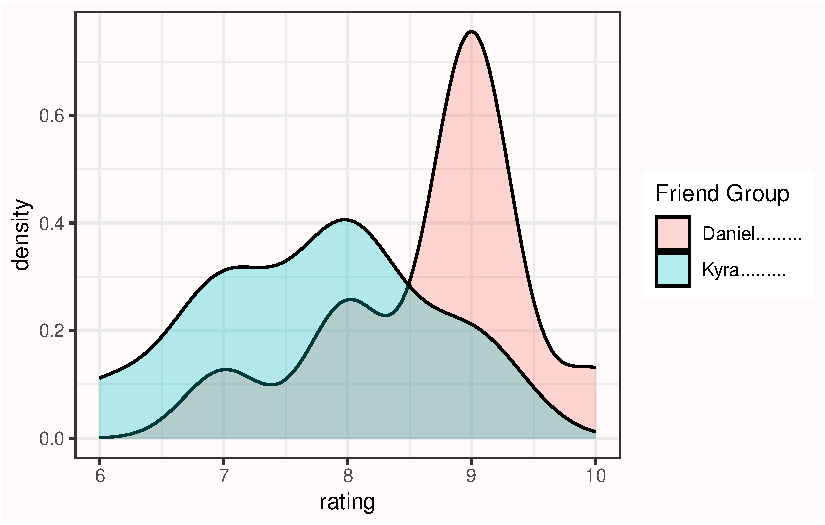
\includegraphics[width=1\textwidth,height=\textheight]{01-pvalue_files/figure-pdf/unnamed-chunk-3-1.pdf}

}

\end{figure}

我们可以看到两组人的数据是重叠的,但平均评分却相差1整分。所以,我们现在面临的问题如下:
两组之间的差异只是随机误差,还是说我的朋友比我妻子的朋友更喜欢《指环王》(LOTR)三部曲的加长版?

在\textbf{零假设的显著性检验}中,我们试图量化所观察到的差异(这时的均值相差1)或更极端差异的概率来回答这个问题,但这个前提是我的朋友和我妻子的朋友对《指环王》加长版的喜好程度并没有真正的差异,而我们只是在察看随机差异。这个概率称为\emph{p}值。如果这个概率足够低,那我们就可以说存在差异,如果这个概率不够低,那我们只能说不存在差异。

零假设假定如果询问了无限多的朋友(我的朋友以及和我妻子的朋友两个组)他们有多喜欢指环王,这两个海量的群组之间的差异为0。然而,从任何总体中抽取某一样本,随机误差通常不为0。我们可以建立一个\textbf{零模型}来衡量所得观测数据的期望误差,如果只有随机误差,那就可以知道合理的期望将会是如何,即当总体之间没有实质差异时,组间的随机误差有多大。

使用\textbf{标准化}分布来建立一个零模型是很便捷的,因为这样计算某一值的概率相对更容易,且不用考虑其余维度。有一个衡量差异的零模型是t分布,它可以用于描绘从总体抽样时的差异情况。有一个衡量差异的零模型是t分布,它可以用于描绘从总体抽样时的差异情况。这种零模型是建立在某种\textbf{假设}之上的。在\emph{t}分布的情况下,这个假设的分布属于正态分布。然而事实上,依据统计方法所提出的假设从来没有得到过完美的匹配,所以,这就是为什么统计学家们在探索违反假设对方法论的影响。当违反假设对统计推断的影响足够小时,那么统计检验的方法仍然是有效且实用的。

我们可以通过\emph{概率密度函数}来衡量当总体中不存在差异时的预期\emph{t}值分布。下面是一个\textbf{自由度}(df)为18的\emph{t}分布的概率密度函数图,它与我们的例子一致,即对应我们从20个朋友那里收集的数据(df=N-2,两个独立组)。对于连续分布来说,概率是由无限多的点定义的,任何一个点的概率(例如,\emph{t}=2.5)总是零。概率是按区间测量的。因此,计算的\emph{p}值并不是所得观测数据(即某一点)的概率,而是所得观测数据\emph{或更极端数据}(即一个区间)的概率。这就形成了一个可以计算面积的概率区间。

\hypertarget{ux8ba1ux7b97pux503c}{%
\section{\texorpdfstring{计算\emph{p}值}{计算p值}}\label{ux8ba1ux7b97pux503c}}

\emph{t}值可以用样本均值、总体均值、样本的标准差和样本大小来计算。然后计算所得观测数据或更极端数据的\emph{t}值概率,我们就得到了\emph{p}值。将上述两组朋友的电影评分进行对比,依据双侧\emph{t}检验可得到的\emph{t}值为2.5175,\emph{p}值为0.02151。

\begin{Shaded}
\begin{Highlighting}[]
\FunctionTok{t.test}\NormalTok{(df\_long}\SpecialCharTok{$}\NormalTok{rating }\SpecialCharTok{\textasciitilde{}}\NormalTok{ df\_long}\SpecialCharTok{$}\StringTok{\textasciigrave{}}\AttributeTok{Friend Group}\StringTok{\textasciigrave{}}\NormalTok{, }\AttributeTok{var.equal =} \ConstantTok{TRUE}\NormalTok{)}
\end{Highlighting}
\end{Shaded}

\begin{verbatim}

    Two Sample t-test

data:  df_long$rating by df_long$`Friend Group`
t = 2.5175, df = 18, p-value = 0.02151
alternative hypothesis: true difference in means between group Daniel的朋友 and group Kyra的朋友 is not equal to 0
95 percent confidence interval:
 0.1654875 1.8345125
sample estimates:
mean in group Daniel的朋友   mean in group Kyra的朋友 
                       8.7                        7.7 
\end{verbatim}

我们可以绘制出\emph{t}分布图(df=18),并高亮了\emph{t}值为2.5175和-2.5175的两个尾部区域。

\begin{verbatim}
Warning in title(...): conversion failure on 't值分布' in 'mbcsToSbcs': dot
substituted for <e5>
\end{verbatim}

\begin{verbatim}
Warning in title(...): conversion failure on 't值分布' in 'mbcsToSbcs': dot
substituted for <80>
\end{verbatim}

\begin{verbatim}
Warning in title(...): conversion failure on 't值分布' in 'mbcsToSbcs': dot
substituted for <bc>
\end{verbatim}

\begin{verbatim}
Warning in title(...): conversion failure on 't值分布' in 'mbcsToSbcs': dot
substituted for <e5>
\end{verbatim}

\begin{verbatim}
Warning in title(...): conversion failure on 't值分布' in 'mbcsToSbcs': dot
substituted for <88>
\end{verbatim}

\begin{verbatim}
Warning in title(...): conversion failure on 't值分布' in 'mbcsToSbcs': dot
substituted for <86>
\end{verbatim}

\begin{verbatim}
Warning in title(...): conversion failure on 't值分布' in 'mbcsToSbcs': dot
substituted for <e5>
\end{verbatim}

\begin{verbatim}
Warning in title(...): conversion failure on 't值分布' in 'mbcsToSbcs': dot
substituted for <b8>
\end{verbatim}

\begin{verbatim}
Warning in title(...): conversion failure on 't值分布' in 'mbcsToSbcs': dot
substituted for <83>
\end{verbatim}

\begin{verbatim}
Warning in title(...): conversion failure on 't值' in 'mbcsToSbcs': dot
substituted for <e5>
\end{verbatim}

\begin{verbatim}
Warning in title(...): conversion failure on 't值' in 'mbcsToSbcs': dot
substituted for <80>
\end{verbatim}

\begin{verbatim}
Warning in title(...): conversion failure on 't值' in 'mbcsToSbcs': dot
substituted for <bc>
\end{verbatim}

\begin{verbatim}
Warning in title(...): conversion failure on '概率密度' in 'mbcsToSbcs': dot
substituted for <e6>
\end{verbatim}

\begin{verbatim}
Warning in title(...): conversion failure on '概率密度' in 'mbcsToSbcs': dot
substituted for <a6>
\end{verbatim}

\begin{verbatim}
Warning in title(...): conversion failure on '概率密度' in 'mbcsToSbcs': dot
substituted for <82>
\end{verbatim}

\begin{verbatim}
Warning in title(...): conversion failure on '概率密度' in 'mbcsToSbcs': dot
substituted for <e7>
\end{verbatim}

\begin{verbatim}
Warning in title(...): conversion failure on '概率密度' in 'mbcsToSbcs': dot
substituted for <8e>
\end{verbatim}

\begin{verbatim}
Warning in title(...): conversion failure on '概率密度' in 'mbcsToSbcs': dot
substituted for <87>
\end{verbatim}

\begin{verbatim}
Warning in title(...): conversion failure on '概率密度' in 'mbcsToSbcs': dot
substituted for <e5>
\end{verbatim}

\begin{verbatim}
Warning in title(...): conversion failure on '概率密度' in 'mbcsToSbcs': dot
substituted for <af>
\end{verbatim}

\begin{verbatim}
Warning in title(...): conversion failure on '概率密度' in 'mbcsToSbcs': dot
substituted for <86>
\end{verbatim}

\begin{verbatim}
Warning in title(...): conversion failure on '概率密度' in 'mbcsToSbcs': dot
substituted for <e5>
\end{verbatim}

\begin{verbatim}
Warning in title(...): conversion failure on '概率密度' in 'mbcsToSbcs': dot
substituted for <ba>
\end{verbatim}

\begin{verbatim}
Warning in title(...): conversion failure on '概率密度' in 'mbcsToSbcs': dot
substituted for <a6>
\end{verbatim}

\begin{figure}

{\centering 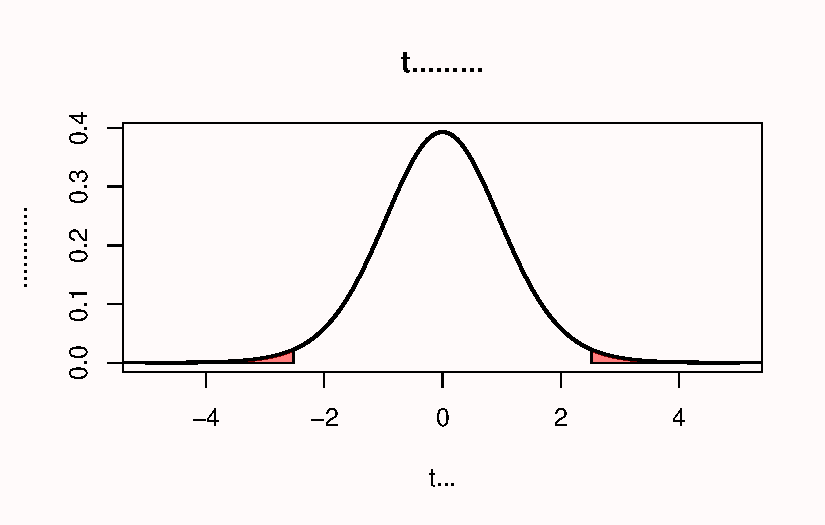
\includegraphics[width=1\textwidth,height=\textheight]{01-pvalue_files/figure-pdf/fig-tdist-1.pdf}

}

\caption{\label{fig-tdist}自由度为18的\emph{t}分布}

\end{figure}

\hypertarget{sec-whichpexpect}{%
\section{哪个是你想要的p值}\label{sec-whichpexpect}}

有一个非常有教学意义的视频叫``\href{https://www.youtube.com/watch?v=5OL1RqHrZQ8}{\emph{p}值之舞}'',Geoff
Cumming觉得p值因实验的不同而有所差异。然而,这并不是他在视频中提到的
``不信任p值''的理由。相反,他认为重要的是要清楚地了解\emph{p}值是如何分布的,以防止误用。因为\emph{p}值是统计中频率学派的部分,我们需要研究的是\emph{从长远来看}能预期得到什么。因为我们永远不会成千上万次的做一个实验,而且我们也无法将所有的时间精力投入至研究中,所以最好的办法就是通过计算模拟求得一个长远的结果。

请大家花一些时间思考一下两个问题。如果效应真实存在,并且你重复这个实验成千上万次了,你可能会得到一个什么样的\emph{p}值?同样,如果效应并不存在,你也同样重复这个实验成千上万次了,你又会得到什么样的\emph{p}值?如果你不知道答案也没有关系,你现在就能学会。如果你不知道答案,或许应该值得反思一下,为什么并不了解\emph{p}值的基本知识。如果你和我一样,根本没有被教过这个。但正如我们将看到的,这对巩固理解\emph{p}值该如何解释至关重要。

你能期望的\emph{p}值完全由研究的统计功效决定,或者说,如果效应真实存在,你将得到显著效应的概率。统计功效的范围在0\textasciitilde1。我们可以通过模拟独立\emph{t}检验来说明这一点。比如说,我们来模拟一群人的智商分数。我们知道智商的标准差是15。现在,我们假设某个样本组的平均智商为100,而另一个组为105。随后,我们来检验这两组人的IQ是否不一致(但是我们知道正确答案是``是'',因为我们就是这么模拟的数据)。

\begin{Shaded}
\begin{Highlighting}[]
\NormalTok{p }\OtherTok{\textless{}{-}} \FunctionTok{numeric}\NormalTok{(}\DecValTok{100000}\NormalTok{) }\CommentTok{\# store all simulated *p*{-}values}

\ControlFlowTok{for}\NormalTok{ (i }\ControlFlowTok{in} \DecValTok{1}\SpecialCharTok{:}\DecValTok{100000}\NormalTok{) \{ }\CommentTok{\# for each simulated experiment}
\NormalTok{  x }\OtherTok{\textless{}{-}} \FunctionTok{rnorm}\NormalTok{(}\AttributeTok{n =} \DecValTok{71}\NormalTok{, }\AttributeTok{mean =} \DecValTok{100}\NormalTok{, }\AttributeTok{sd =} \DecValTok{15}\NormalTok{) }\CommentTok{\# Simulate data}
\NormalTok{  y }\OtherTok{\textless{}{-}} \FunctionTok{rnorm}\NormalTok{(}\AttributeTok{n =} \DecValTok{71}\NormalTok{, }\AttributeTok{mean =} \DecValTok{105}\NormalTok{, }\AttributeTok{sd =} \DecValTok{15}\NormalTok{) }\CommentTok{\# Simulate data}
\NormalTok{  p[i] }\OtherTok{\textless{}{-}} \FunctionTok{t.test}\NormalTok{(x, y)}\SpecialCharTok{$}\NormalTok{p.value }\CommentTok{\# store the *p*{-}value}
\NormalTok{\}}

\NormalTok{(}\FunctionTok{sum}\NormalTok{(p }\SpecialCharTok{\textless{}} \FloatTok{0.05}\NormalTok{) }\SpecialCharTok{/} \DecValTok{100000}\NormalTok{) }\CommentTok{\# compute power}

\FunctionTok{hist}\NormalTok{(p, }\AttributeTok{breaks =} \DecValTok{20}\NormalTok{) }\CommentTok{\# plot a histogram}
\end{Highlighting}
\end{Shaded}

在模拟时,我们生成了一个关于IQ分数的正态分布(n =
71,均值M=100或105),标准差=15)。然后我们进行独立t检验,求得p值,并生成\emph{p}值分布图。

\begin{verbatim}
Warning in title(main = main, sub = sub, xlab = xlab, ylab = ylab, ...):
conversion failure on '50%功效下的p值分布' in 'mbcsToSbcs': dot substituted for
<e5>
\end{verbatim}

\begin{verbatim}
Warning in title(main = main, sub = sub, xlab = xlab, ylab = ylab, ...):
conversion failure on '50%功效下的p值分布' in 'mbcsToSbcs': dot substituted for
<8a>
\end{verbatim}

\begin{verbatim}
Warning in title(main = main, sub = sub, xlab = xlab, ylab = ylab, ...):
conversion failure on '50%功效下的p值分布' in 'mbcsToSbcs': dot substituted for
<9f>
\end{verbatim}

\begin{verbatim}
Warning in title(main = main, sub = sub, xlab = xlab, ylab = ylab, ...):
conversion failure on '50%功效下的p值分布' in 'mbcsToSbcs': dot substituted for
<e6>
\end{verbatim}

\begin{verbatim}
Warning in title(main = main, sub = sub, xlab = xlab, ylab = ylab, ...):
conversion failure on '50%功效下的p值分布' in 'mbcsToSbcs': dot substituted for
<95>
\end{verbatim}

\begin{verbatim}
Warning in title(main = main, sub = sub, xlab = xlab, ylab = ylab, ...):
conversion failure on '50%功效下的p值分布' in 'mbcsToSbcs': dot substituted for
<88>
\end{verbatim}

\begin{verbatim}
Warning in title(main = main, sub = sub, xlab = xlab, ylab = ylab, ...):
conversion failure on '50%功效下的p值分布' in 'mbcsToSbcs': dot substituted for
<e4>
\end{verbatim}

\begin{verbatim}
Warning in title(main = main, sub = sub, xlab = xlab, ylab = ylab, ...):
conversion failure on '50%功效下的p值分布' in 'mbcsToSbcs': dot substituted for
<b8>
\end{verbatim}

\begin{verbatim}
Warning in title(main = main, sub = sub, xlab = xlab, ylab = ylab, ...):
conversion failure on '50%功效下的p值分布' in 'mbcsToSbcs': dot substituted for
<8b>
\end{verbatim}

\begin{verbatim}
Warning in title(main = main, sub = sub, xlab = xlab, ylab = ylab, ...):
conversion failure on '50%功效下的p值分布' in 'mbcsToSbcs': dot substituted for
<e7>
\end{verbatim}

\begin{verbatim}
Warning in title(main = main, sub = sub, xlab = xlab, ylab = ylab, ...):
conversion failure on '50%功效下的p值分布' in 'mbcsToSbcs': dot substituted for
<9a>
\end{verbatim}

\begin{verbatim}
Warning in title(main = main, sub = sub, xlab = xlab, ylab = ylab, ...):
conversion failure on '50%功效下的p值分布' in 'mbcsToSbcs': dot substituted for
<84>
\end{verbatim}

\begin{verbatim}
Warning in title(main = main, sub = sub, xlab = xlab, ylab = ylab, ...):
conversion failure on '50%功效下的p值分布' in 'mbcsToSbcs': dot substituted for
<e5>
\end{verbatim}

\begin{verbatim}
Warning in title(main = main, sub = sub, xlab = xlab, ylab = ylab, ...):
conversion failure on '50%功效下的p值分布' in 'mbcsToSbcs': dot substituted for
<80>
\end{verbatim}

\begin{verbatim}
Warning in title(main = main, sub = sub, xlab = xlab, ylab = ylab, ...):
conversion failure on '50%功效下的p值分布' in 'mbcsToSbcs': dot substituted for
<bc>
\end{verbatim}

\begin{verbatim}
Warning in title(main = main, sub = sub, xlab = xlab, ylab = ylab, ...):
conversion failure on '50%功效下的p值分布' in 'mbcsToSbcs': dot substituted for
<e5>
\end{verbatim}

\begin{verbatim}
Warning in title(main = main, sub = sub, xlab = xlab, ylab = ylab, ...):
conversion failure on '50%功效下的p值分布' in 'mbcsToSbcs': dot substituted for
<88>
\end{verbatim}

\begin{verbatim}
Warning in title(main = main, sub = sub, xlab = xlab, ylab = ylab, ...):
conversion failure on '50%功效下的p值分布' in 'mbcsToSbcs': dot substituted for
<86>
\end{verbatim}

\begin{verbatim}
Warning in title(main = main, sub = sub, xlab = xlab, ylab = ylab, ...):
conversion failure on '50%功效下的p值分布' in 'mbcsToSbcs': dot substituted for
<e5>
\end{verbatim}

\begin{verbatim}
Warning in title(main = main, sub = sub, xlab = xlab, ylab = ylab, ...):
conversion failure on '50%功效下的p值分布' in 'mbcsToSbcs': dot substituted for
<b8>
\end{verbatim}

\begin{verbatim}
Warning in title(main = main, sub = sub, xlab = xlab, ylab = ylab, ...):
conversion failure on '50%功效下的p值分布' in 'mbcsToSbcs': dot substituted for
<83>
\end{verbatim}

\begin{verbatim}
Warning in title(main = main, sub = sub, xlab = xlab, ylab = ylab, ...):
conversion failure on 'P值' in 'mbcsToSbcs': dot substituted for <e5>
\end{verbatim}

\begin{verbatim}
Warning in title(main = main, sub = sub, xlab = xlab, ylab = ylab, ...):
conversion failure on 'P值' in 'mbcsToSbcs': dot substituted for <80>
\end{verbatim}

\begin{verbatim}
Warning in title(main = main, sub = sub, xlab = xlab, ylab = ylab, ...):
conversion failure on 'P值' in 'mbcsToSbcs': dot substituted for <bc>
\end{verbatim}

\begin{verbatim}
Warning in title(main = main, sub = sub, xlab = xlab, ylab = ylab, ...):
conversion failure on 'p值的数量' in 'mbcsToSbcs': dot substituted for <e5>
\end{verbatim}

\begin{verbatim}
Warning in title(main = main, sub = sub, xlab = xlab, ylab = ylab, ...):
conversion failure on 'p值的数量' in 'mbcsToSbcs': dot substituted for <80>
\end{verbatim}

\begin{verbatim}
Warning in title(main = main, sub = sub, xlab = xlab, ylab = ylab, ...):
conversion failure on 'p值的数量' in 'mbcsToSbcs': dot substituted for <bc>
\end{verbatim}

\begin{verbatim}
Warning in title(main = main, sub = sub, xlab = xlab, ylab = ylab, ...):
conversion failure on 'p值的数量' in 'mbcsToSbcs': dot substituted for <e7>
\end{verbatim}

\begin{verbatim}
Warning in title(main = main, sub = sub, xlab = xlab, ylab = ylab, ...):
conversion failure on 'p值的数量' in 'mbcsToSbcs': dot substituted for <9a>
\end{verbatim}

\begin{verbatim}
Warning in title(main = main, sub = sub, xlab = xlab, ylab = ylab, ...):
conversion failure on 'p值的数量' in 'mbcsToSbcs': dot substituted for <84>
\end{verbatim}

\begin{verbatim}
Warning in title(main = main, sub = sub, xlab = xlab, ylab = ylab, ...):
conversion failure on 'p值的数量' in 'mbcsToSbcs': dot substituted for <e6>
\end{verbatim}

\begin{verbatim}
Warning in title(main = main, sub = sub, xlab = xlab, ylab = ylab, ...):
conversion failure on 'p值的数量' in 'mbcsToSbcs': dot substituted for <95>
\end{verbatim}

\begin{verbatim}
Warning in title(main = main, sub = sub, xlab = xlab, ylab = ylab, ...):
conversion failure on 'p值的数量' in 'mbcsToSbcs': dot substituted for <b0>
\end{verbatim}

\begin{verbatim}
Warning in title(main = main, sub = sub, xlab = xlab, ylab = ylab, ...):
conversion failure on 'p值的数量' in 'mbcsToSbcs': dot substituted for <e9>
\end{verbatim}

\begin{verbatim}
Warning in title(main = main, sub = sub, xlab = xlab, ylab = ylab, ...):
conversion failure on 'p值的数量' in 'mbcsToSbcs': dot substituted for <87>
\end{verbatim}

\begin{verbatim}
Warning in title(main = main, sub = sub, xlab = xlab, ylab = ylab, ...):
conversion failure on 'p值的数量' in 'mbcsToSbcs': dot substituted for <8f>
\end{verbatim}

\begin{figure}

{\centering 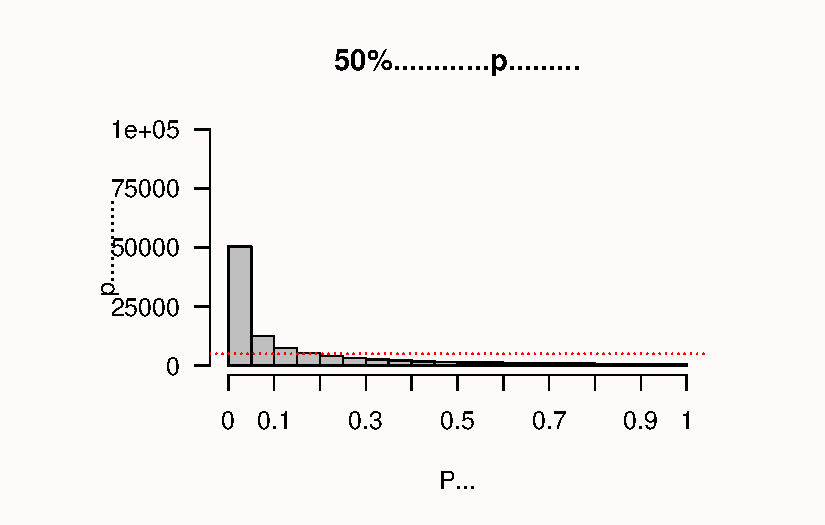
\includegraphics[width=1\textwidth,height=\textheight]{01-pvalue_files/figure-pdf/fig-pdistr1-1.pdf}

}

\caption{\label{fig-pdistr1}统计检验力为50\%时的\emph{p}分布}

\end{figure}

我们可以看到x轴是20个条形柱分别代表着从0到1的\emph{p}值,Y轴则是这些\emph{p}值的频率。水平的红色虚线表示5\%的\(\alpha\)(位于100.000*0.05=5000的频率),但你现在可以忽略这条线。图表的标题给出了模拟研究的统计功效(假设\(\alpha\)为0.05时):
这项研究有50\%的功效。

模拟的结果描绘了\emph{p}值的\emph{概率密度函数}。概率密度函数给出了在\emph{t}分布中,某个特定值(比如如图@fig-tdist那样)的随机变量的概率。因为\emph{p}值是一个随机变量,我们可以用它的概率密度函数来绘制\emph{p}值分布图(Hung
et al., 1997; Ulrich \& Miller,
2018),如图@fig-pdft。在\href{http://shiny.ieis.tue.nl/d_p_power/}{线上的Shiny应用程序}中,你可以改变样本大小、效应量大小和\(\alpha\)水平,以便观察他们对\emph{p}值分布的影响。增加样本量或效应量大小将增加\emph{p}值分布的陡峭程度,这意味着观察到小\emph{p}值的概率增加。\emph{p}值分布是检验的统计功效的函数。

\begin{verbatim}
Warning in title(...): conversion failure on 'p值分布' in 'mbcsToSbcs': dot
substituted for <e5>
\end{verbatim}

\begin{verbatim}
Warning in title(...): conversion failure on 'p值分布' in 'mbcsToSbcs': dot
substituted for <80>
\end{verbatim}

\begin{verbatim}
Warning in title(...): conversion failure on 'p值分布' in 'mbcsToSbcs': dot
substituted for <bc>
\end{verbatim}

\begin{verbatim}
Warning in title(...): conversion failure on 'p值分布' in 'mbcsToSbcs': dot
substituted for <e5>
\end{verbatim}

\begin{verbatim}
Warning in title(...): conversion failure on 'p值分布' in 'mbcsToSbcs': dot
substituted for <88>
\end{verbatim}

\begin{verbatim}
Warning in title(...): conversion failure on 'p值分布' in 'mbcsToSbcs': dot
substituted for <86>
\end{verbatim}

\begin{verbatim}
Warning in title(...): conversion failure on 'p值分布' in 'mbcsToSbcs': dot
substituted for <e5>
\end{verbatim}

\begin{verbatim}
Warning in title(...): conversion failure on 'p值分布' in 'mbcsToSbcs': dot
substituted for <b8>
\end{verbatim}

\begin{verbatim}
Warning in title(...): conversion failure on 'p值分布' in 'mbcsToSbcs': dot
substituted for <83>
\end{verbatim}

\begin{verbatim}
Warning in title(...): conversion failure on 'p值' in 'mbcsToSbcs': dot
substituted for <e5>
\end{verbatim}

\begin{verbatim}
Warning in title(...): conversion failure on 'p值' in 'mbcsToSbcs': dot
substituted for <80>
\end{verbatim}

\begin{verbatim}
Warning in title(...): conversion failure on 'p值' in 'mbcsToSbcs': dot
substituted for <bc>
\end{verbatim}

\begin{verbatim}
Warning in title(...): conversion failure on '概率密度' in 'mbcsToSbcs': dot
substituted for <e6>
\end{verbatim}

\begin{verbatim}
Warning in title(...): conversion failure on '概率密度' in 'mbcsToSbcs': dot
substituted for <a6>
\end{verbatim}

\begin{verbatim}
Warning in title(...): conversion failure on '概率密度' in 'mbcsToSbcs': dot
substituted for <82>
\end{verbatim}

\begin{verbatim}
Warning in title(...): conversion failure on '概率密度' in 'mbcsToSbcs': dot
substituted for <e7>
\end{verbatim}

\begin{verbatim}
Warning in title(...): conversion failure on '概率密度' in 'mbcsToSbcs': dot
substituted for <8e>
\end{verbatim}

\begin{verbatim}
Warning in title(...): conversion failure on '概率密度' in 'mbcsToSbcs': dot
substituted for <87>
\end{verbatim}

\begin{verbatim}
Warning in title(...): conversion failure on '概率密度' in 'mbcsToSbcs': dot
substituted for <e5>
\end{verbatim}

\begin{verbatim}
Warning in title(...): conversion failure on '概率密度' in 'mbcsToSbcs': dot
substituted for <af>
\end{verbatim}

\begin{verbatim}
Warning in title(...): conversion failure on '概率密度' in 'mbcsToSbcs': dot
substituted for <86>
\end{verbatim}

\begin{verbatim}
Warning in title(...): conversion failure on '概率密度' in 'mbcsToSbcs': dot
substituted for <e5>
\end{verbatim}

\begin{verbatim}
Warning in title(...): conversion failure on '概率密度' in 'mbcsToSbcs': dot
substituted for <ba>
\end{verbatim}

\begin{verbatim}
Warning in title(...): conversion failure on '概率密度' in 'mbcsToSbcs': dot
substituted for <a6>
\end{verbatim}

\begin{figure}

{\centering 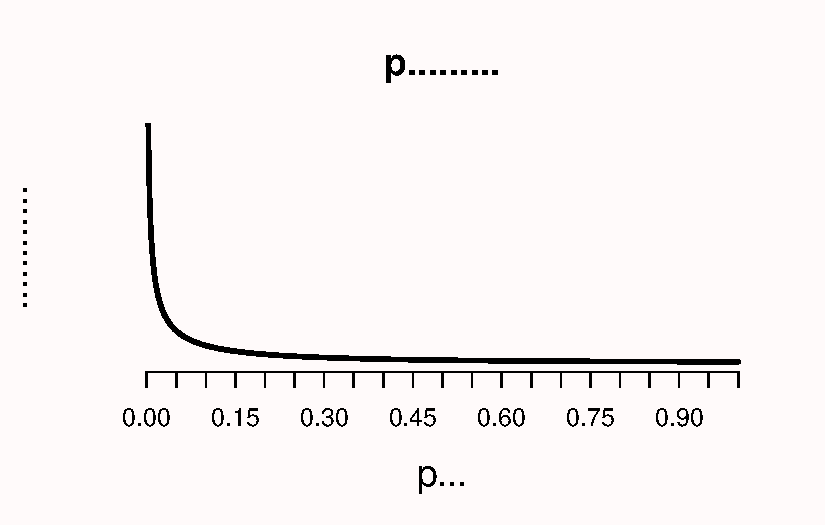
\includegraphics[width=1\textwidth,height=\textheight]{01-pvalue_files/figure-pdf/fig-pdft-1.pdf}

}

\caption{\label{fig-pdft}一个双侧\emph{t}检验对应的\emph{p}值概率密度函数}

\end{figure}

当效应不存在时,\emph{p}值是\textbf{均匀分布}的。这意味着,当零假设为真时,每一个\emph{p}值都有同样的可能性被观察到。换句话说,当不存在真正的效应时,0.08的\emph{p}值和0.98的\emph{p}值含义一样。我记得当我第一次了解到均匀的\emph{p}值分布时,我觉得这非常反常(远在完成我的博士学位之上)。但是如果保证零假设为真,\emph{p}值永远大于我们所设定的\(\alpha\)水平时,那么\emph{p}值为均匀分布似乎又是合理的。如果我们把\(\alpha\)水平设为0.01,1\%的概率观察到的\emph{p}值小于0.01,如果我们把\(\alpha\)水平设置为0.12,12\%的概率观察到\emph{p}值小于0.12。但是,这只有在零假设(\(H_0\))为真时,\emph{p}值是均匀分布的情况下才会发生这种情况。

\begin{verbatim}
Warning in title(main = main, sub = sub, xlab = xlab, ylab = ylab, ...):
conversion failure on '当零假设为真时的p值分布' in 'mbcsToSbcs': dot
substituted for <e5>
\end{verbatim}

\begin{verbatim}
Warning in title(main = main, sub = sub, xlab = xlab, ylab = ylab, ...):
conversion failure on '当零假设为真时的p值分布' in 'mbcsToSbcs': dot
substituted for <bd>
\end{verbatim}

\begin{verbatim}
Warning in title(main = main, sub = sub, xlab = xlab, ylab = ylab, ...):
conversion failure on '当零假设为真时的p值分布' in 'mbcsToSbcs': dot
substituted for <93>
\end{verbatim}

\begin{verbatim}
Warning in title(main = main, sub = sub, xlab = xlab, ylab = ylab, ...):
conversion failure on '当零假设为真时的p值分布' in 'mbcsToSbcs': dot
substituted for <e9>
\end{verbatim}

\begin{verbatim}
Warning in title(main = main, sub = sub, xlab = xlab, ylab = ylab, ...):
conversion failure on '当零假设为真时的p值分布' in 'mbcsToSbcs': dot
substituted for <9b>
\end{verbatim}

\begin{verbatim}
Warning in title(main = main, sub = sub, xlab = xlab, ylab = ylab, ...):
conversion failure on '当零假设为真时的p值分布' in 'mbcsToSbcs': dot
substituted for <b6>
\end{verbatim}

\begin{verbatim}
Warning in title(main = main, sub = sub, xlab = xlab, ylab = ylab, ...):
conversion failure on '当零假设为真时的p值分布' in 'mbcsToSbcs': dot
substituted for <e5>
\end{verbatim}

\begin{verbatim}
Warning in title(main = main, sub = sub, xlab = xlab, ylab = ylab, ...):
conversion failure on '当零假设为真时的p值分布' in 'mbcsToSbcs': dot
substituted for <81>
\end{verbatim}

\begin{verbatim}
Warning in title(main = main, sub = sub, xlab = xlab, ylab = ylab, ...):
conversion failure on '当零假设为真时的p值分布' in 'mbcsToSbcs': dot
substituted for <87>
\end{verbatim}

\begin{verbatim}
Warning in title(main = main, sub = sub, xlab = xlab, ylab = ylab, ...):
conversion failure on '当零假设为真时的p值分布' in 'mbcsToSbcs': dot
substituted for <e8>
\end{verbatim}

\begin{verbatim}
Warning in title(main = main, sub = sub, xlab = xlab, ylab = ylab, ...):
conversion failure on '当零假设为真时的p值分布' in 'mbcsToSbcs': dot
substituted for <ae>
\end{verbatim}

\begin{verbatim}
Warning in title(main = main, sub = sub, xlab = xlab, ylab = ylab, ...):
conversion failure on '当零假设为真时的p值分布' in 'mbcsToSbcs': dot
substituted for <be>
\end{verbatim}

\begin{verbatim}
Warning in title(main = main, sub = sub, xlab = xlab, ylab = ylab, ...):
conversion failure on '当零假设为真时的p值分布' in 'mbcsToSbcs': dot
substituted for <e4>
\end{verbatim}

\begin{verbatim}
Warning in title(main = main, sub = sub, xlab = xlab, ylab = ylab, ...):
conversion failure on '当零假设为真时的p值分布' in 'mbcsToSbcs': dot
substituted for <b8>
\end{verbatim}

\begin{verbatim}
Warning in title(main = main, sub = sub, xlab = xlab, ylab = ylab, ...):
conversion failure on '当零假设为真时的p值分布' in 'mbcsToSbcs': dot
substituted for <ba>
\end{verbatim}

\begin{verbatim}
Warning in title(main = main, sub = sub, xlab = xlab, ylab = ylab, ...):
conversion failure on '当零假设为真时的p值分布' in 'mbcsToSbcs': dot
substituted for <e7>
\end{verbatim}

\begin{verbatim}
Warning in title(main = main, sub = sub, xlab = xlab, ylab = ylab, ...):
conversion failure on '当零假设为真时的p值分布' in 'mbcsToSbcs': dot
substituted for <9c>
\end{verbatim}

\begin{verbatim}
Warning in title(main = main, sub = sub, xlab = xlab, ylab = ylab, ...):
conversion failure on '当零假设为真时的p值分布' in 'mbcsToSbcs': dot
substituted for <9f>
\end{verbatim}

\begin{verbatim}
Warning in title(main = main, sub = sub, xlab = xlab, ylab = ylab, ...):
conversion failure on '当零假设为真时的p值分布' in 'mbcsToSbcs': dot
substituted for <e6>
\end{verbatim}

\begin{verbatim}
Warning in title(main = main, sub = sub, xlab = xlab, ylab = ylab, ...):
conversion failure on '当零假设为真时的p值分布' in 'mbcsToSbcs': dot
substituted for <97>
\end{verbatim}

\begin{verbatim}
Warning in title(main = main, sub = sub, xlab = xlab, ylab = ylab, ...):
conversion failure on '当零假设为真时的p值分布' in 'mbcsToSbcs': dot
substituted for <b6>
\end{verbatim}

\begin{verbatim}
Warning in title(main = main, sub = sub, xlab = xlab, ylab = ylab, ...):
conversion failure on '当零假设为真时的p值分布' in 'mbcsToSbcs': dot
substituted for <e7>
\end{verbatim}

\begin{verbatim}
Warning in title(main = main, sub = sub, xlab = xlab, ylab = ylab, ...):
conversion failure on '当零假设为真时的p值分布' in 'mbcsToSbcs': dot
substituted for <9a>
\end{verbatim}

\begin{verbatim}
Warning in title(main = main, sub = sub, xlab = xlab, ylab = ylab, ...):
conversion failure on '当零假设为真时的p值分布' in 'mbcsToSbcs': dot
substituted for <84>
\end{verbatim}

\begin{verbatim}
Warning in title(main = main, sub = sub, xlab = xlab, ylab = ylab, ...):
conversion failure on '当零假设为真时的p值分布' in 'mbcsToSbcs': dot
substituted for <e5>
\end{verbatim}

\begin{verbatim}
Warning in title(main = main, sub = sub, xlab = xlab, ylab = ylab, ...):
conversion failure on '当零假设为真时的p值分布' in 'mbcsToSbcs': dot
substituted for <80>
\end{verbatim}

\begin{verbatim}
Warning in title(main = main, sub = sub, xlab = xlab, ylab = ylab, ...):
conversion failure on '当零假设为真时的p值分布' in 'mbcsToSbcs': dot
substituted for <bc>
\end{verbatim}

\begin{verbatim}
Warning in title(main = main, sub = sub, xlab = xlab, ylab = ylab, ...):
conversion failure on '当零假设为真时的p值分布' in 'mbcsToSbcs': dot
substituted for <e5>
\end{verbatim}

\begin{verbatim}
Warning in title(main = main, sub = sub, xlab = xlab, ylab = ylab, ...):
conversion failure on '当零假设为真时的p值分布' in 'mbcsToSbcs': dot
substituted for <88>
\end{verbatim}

\begin{verbatim}
Warning in title(main = main, sub = sub, xlab = xlab, ylab = ylab, ...):
conversion failure on '当零假设为真时的p值分布' in 'mbcsToSbcs': dot
substituted for <86>
\end{verbatim}

\begin{verbatim}
Warning in title(main = main, sub = sub, xlab = xlab, ylab = ylab, ...):
conversion failure on '当零假设为真时的p值分布' in 'mbcsToSbcs': dot
substituted for <e5>
\end{verbatim}

\begin{verbatim}
Warning in title(main = main, sub = sub, xlab = xlab, ylab = ylab, ...):
conversion failure on '当零假设为真时的p值分布' in 'mbcsToSbcs': dot
substituted for <b8>
\end{verbatim}

\begin{verbatim}
Warning in title(main = main, sub = sub, xlab = xlab, ylab = ylab, ...):
conversion failure on '当零假设为真时的p值分布' in 'mbcsToSbcs': dot
substituted for <83>
\end{verbatim}

\begin{verbatim}
Warning in title(main = main, sub = sub, xlab = xlab, ylab = ylab, ...):
conversion failure on 'p值' in 'mbcsToSbcs': dot substituted for <e5>
\end{verbatim}

\begin{verbatim}
Warning in title(main = main, sub = sub, xlab = xlab, ylab = ylab, ...):
conversion failure on 'p值' in 'mbcsToSbcs': dot substituted for <80>
\end{verbatim}

\begin{verbatim}
Warning in title(main = main, sub = sub, xlab = xlab, ylab = ylab, ...):
conversion failure on 'p值' in 'mbcsToSbcs': dot substituted for <bc>
\end{verbatim}

\begin{verbatim}
Warning in title(main = main, sub = sub, xlab = xlab, ylab = ylab, ...):
conversion failure on 'p值的数量' in 'mbcsToSbcs': dot substituted for <e5>
\end{verbatim}

\begin{verbatim}
Warning in title(main = main, sub = sub, xlab = xlab, ylab = ylab, ...):
conversion failure on 'p值的数量' in 'mbcsToSbcs': dot substituted for <80>
\end{verbatim}

\begin{verbatim}
Warning in title(main = main, sub = sub, xlab = xlab, ylab = ylab, ...):
conversion failure on 'p值的数量' in 'mbcsToSbcs': dot substituted for <bc>
\end{verbatim}

\begin{verbatim}
Warning in title(main = main, sub = sub, xlab = xlab, ylab = ylab, ...):
conversion failure on 'p值的数量' in 'mbcsToSbcs': dot substituted for <e7>
\end{verbatim}

\begin{verbatim}
Warning in title(main = main, sub = sub, xlab = xlab, ylab = ylab, ...):
conversion failure on 'p值的数量' in 'mbcsToSbcs': dot substituted for <9a>
\end{verbatim}

\begin{verbatim}
Warning in title(main = main, sub = sub, xlab = xlab, ylab = ylab, ...):
conversion failure on 'p值的数量' in 'mbcsToSbcs': dot substituted for <84>
\end{verbatim}

\begin{verbatim}
Warning in title(main = main, sub = sub, xlab = xlab, ylab = ylab, ...):
conversion failure on 'p值的数量' in 'mbcsToSbcs': dot substituted for <e6>
\end{verbatim}

\begin{verbatim}
Warning in title(main = main, sub = sub, xlab = xlab, ylab = ylab, ...):
conversion failure on 'p值的数量' in 'mbcsToSbcs': dot substituted for <95>
\end{verbatim}

\begin{verbatim}
Warning in title(main = main, sub = sub, xlab = xlab, ylab = ylab, ...):
conversion failure on 'p值的数量' in 'mbcsToSbcs': dot substituted for <b0>
\end{verbatim}

\begin{verbatim}
Warning in title(main = main, sub = sub, xlab = xlab, ylab = ylab, ...):
conversion failure on 'p值的数量' in 'mbcsToSbcs': dot substituted for <e9>
\end{verbatim}

\begin{verbatim}
Warning in title(main = main, sub = sub, xlab = xlab, ylab = ylab, ...):
conversion failure on 'p值的数量' in 'mbcsToSbcs': dot substituted for <87>
\end{verbatim}

\begin{verbatim}
Warning in title(main = main, sub = sub, xlab = xlab, ylab = ylab, ...):
conversion failure on 'p值的数量' in 'mbcsToSbcs': dot substituted for <8f>
\end{verbatim}

\begin{figure}

{\centering 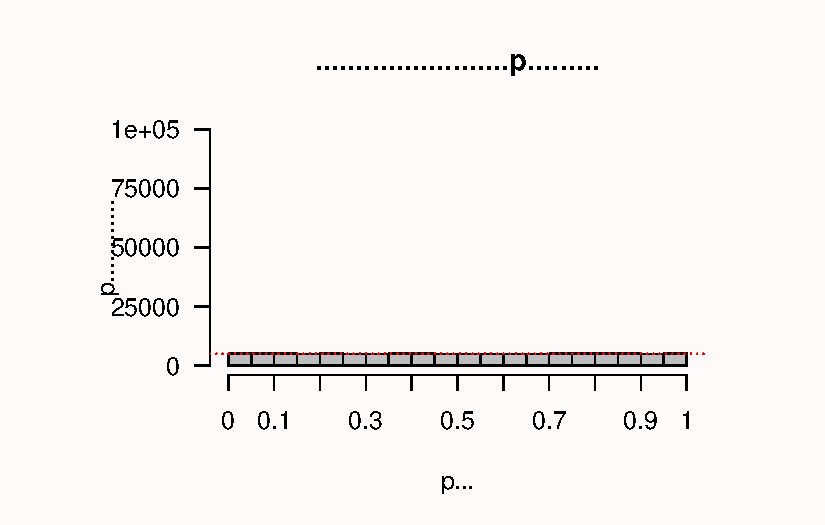
\includegraphics[width=1\textwidth,height=\textheight]{01-pvalue_files/figure-pdf/fig-pdistr2-1.pdf}

}

\caption{\label{fig-pdistr2}零假设为真时的\emph{p}值分布}

\end{figure}

\hypertarget{sec-lindley}{%
\section{林德利悖论}\label{sec-lindley}}

随着统计功效的提高,一些稍微低于0.05的\emph{p}值(如\emph{p}=0.04),相比于\emph{有}效应,它更可能在\emph{没有}效应时出现。这就是著名的林德利悖论
(Lindley, 1957),或称杰弗里-林德利悖论 (Spanos,
2013)。因为\emph{p}值的分布是统计功效的函数 (Cumming,
2008),功效越高,\emph{p}值的分布就越右偏(即越有可能观察到小的\emph{p}值)。当不存在真实的效应时,\emph{p}值是均匀分布的,1\%的概率可以观察到\emph{p}值在0.04和0.05之间。当统计功效极高时,不仅大多数\emph{p}值会低于0.05,甚至会低于0.01。通过图@fig-paradox我们可以看到,在高功效下,当效应\emph{真实存在}时,非常小的\emph{p}值(例如0.001)就比\emph{无}效应时更容易被观察到(例如,当P值为0.01时,代表99\%功效的黑色虚线落在灰色水平线之上,这时灰色曲线代表着零假设为真时\emph{p}值的均匀分布)。

然而令人迷惑的是,当\emph{p}值为0.04时,则更可能是没有效应,即零假设(\(H_0\))为真时,我们任然可以有非常高的功效,例如在图@fig-paradox中所示,当\emph{p}等于0.04时,零假设为真时的\emph{p}值分布的密度要比99\%功效时要高。所以,林德利悖论说明,0.04的\emph{p}值可能在统计学上是显著的,但同时也为零假设提供了一定证据。从Neyman-Pearson的方法来看,我们将提出一个最大错误率为5\%的概念,但从似然比或贝叶斯的方法来看,我们可以得出某种结论是:相对于备择假设,我们的数据信息提供了有利于零假设的证据。林德利悖论说明了不同的统计学派何时会得出不同的结论,以及在不考虑检验统计功效的情况下,为什么\emph{p}值不能直接被解释为结论的衡量标准。虽然可能没有必要,但研究者可能希望避免下述情况:那就是频率学派的学者们会根据\emph{p}\textless0.05拒绝零假设,但是当前检验的实验数据倾向于零假设而不是备择假设。这可以通过降低\(\alpha\)水平作一个样本量的函数来实现Good
(1992),这一点将在``\protect\hyperlink{errorcontrol}{误差的控制}''一章节进行解释。

\begin{verbatim}
Warning in title(...): conversion failure on 'd = 0,
50%和99%统计功效下的p值分布' in 'mbcsToSbcs': dot substituted for <e5>
\end{verbatim}

\begin{verbatim}
Warning in title(...): conversion failure on 'd = 0,
50%和99%统计功效下的p值分布' in 'mbcsToSbcs': dot substituted for <92>
\end{verbatim}

\begin{verbatim}
Warning in title(...): conversion failure on 'd = 0,
50%和99%统计功效下的p值分布' in 'mbcsToSbcs': dot substituted for <8c>
\end{verbatim}

\begin{verbatim}
Warning in title(...): conversion failure on 'd = 0,
50%和99%统计功效下的p值分布' in 'mbcsToSbcs': dot substituted for <e7>
\end{verbatim}

\begin{verbatim}
Warning in title(...): conversion failure on 'd = 0,
50%和99%统计功效下的p值分布' in 'mbcsToSbcs': dot substituted for <bb>
\end{verbatim}

\begin{verbatim}
Warning in title(...): conversion failure on 'd = 0,
50%和99%统计功效下的p值分布' in 'mbcsToSbcs': dot substituted for <9f>
\end{verbatim}

\begin{verbatim}
Warning in title(...): conversion failure on 'd = 0,
50%和99%统计功效下的p值分布' in 'mbcsToSbcs': dot substituted for <e8>
\end{verbatim}

\begin{verbatim}
Warning in title(...): conversion failure on 'd = 0,
50%和99%统计功效下的p值分布' in 'mbcsToSbcs': dot substituted for <ae>
\end{verbatim}

\begin{verbatim}
Warning in title(...): conversion failure on 'd = 0,
50%和99%统计功效下的p值分布' in 'mbcsToSbcs': dot substituted for <a1>
\end{verbatim}

\begin{verbatim}
Warning in title(...): conversion failure on 'd = 0,
50%和99%统计功效下的p值分布' in 'mbcsToSbcs': dot substituted for <e5>
\end{verbatim}

\begin{verbatim}
Warning in title(...): conversion failure on 'd = 0,
50%和99%统计功效下的p值分布' in 'mbcsToSbcs': dot substituted for <8a>
\end{verbatim}

\begin{verbatim}
Warning in title(...): conversion failure on 'd = 0,
50%和99%统计功效下的p值分布' in 'mbcsToSbcs': dot substituted for <9f>
\end{verbatim}

\begin{verbatim}
Warning in title(...): conversion failure on 'd = 0,
50%和99%统计功效下的p值分布' in 'mbcsToSbcs': dot substituted for <e6>
\end{verbatim}

\begin{verbatim}
Warning in title(...): conversion failure on 'd = 0,
50%和99%统计功效下的p值分布' in 'mbcsToSbcs': dot substituted for <95>
\end{verbatim}

\begin{verbatim}
Warning in title(...): conversion failure on 'd = 0,
50%和99%统计功效下的p值分布' in 'mbcsToSbcs': dot substituted for <88>
\end{verbatim}

\begin{verbatim}
Warning in title(...): conversion failure on 'd = 0,
50%和99%统计功效下的p值分布' in 'mbcsToSbcs': dot substituted for <e4>
\end{verbatim}

\begin{verbatim}
Warning in title(...): conversion failure on 'd = 0,
50%和99%统计功效下的p值分布' in 'mbcsToSbcs': dot substituted for <b8>
\end{verbatim}

\begin{verbatim}
Warning in title(...): conversion failure on 'd = 0,
50%和99%统计功效下的p值分布' in 'mbcsToSbcs': dot substituted for <8b>
\end{verbatim}

\begin{verbatim}
Warning in title(...): conversion failure on 'd = 0,
50%和99%统计功效下的p值分布' in 'mbcsToSbcs': dot substituted for <e7>
\end{verbatim}

\begin{verbatim}
Warning in title(...): conversion failure on 'd = 0,
50%和99%统计功效下的p值分布' in 'mbcsToSbcs': dot substituted for <9a>
\end{verbatim}

\begin{verbatim}
Warning in title(...): conversion failure on 'd = 0,
50%和99%统计功效下的p值分布' in 'mbcsToSbcs': dot substituted for <84>
\end{verbatim}

\begin{verbatim}
Warning in title(...): conversion failure on 'd = 0,
50%和99%统计功效下的p值分布' in 'mbcsToSbcs': dot substituted for <e5>
\end{verbatim}

\begin{verbatim}
Warning in title(...): conversion failure on 'd = 0,
50%和99%统计功效下的p值分布' in 'mbcsToSbcs': dot substituted for <80>
\end{verbatim}

\begin{verbatim}
Warning in title(...): conversion failure on 'd = 0,
50%和99%统计功效下的p值分布' in 'mbcsToSbcs': dot substituted for <bc>
\end{verbatim}

\begin{verbatim}
Warning in title(...): conversion failure on 'd = 0,
50%和99%统计功效下的p值分布' in 'mbcsToSbcs': dot substituted for <e5>
\end{verbatim}

\begin{verbatim}
Warning in title(...): conversion failure on 'd = 0,
50%和99%统计功效下的p值分布' in 'mbcsToSbcs': dot substituted for <88>
\end{verbatim}

\begin{verbatim}
Warning in title(...): conversion failure on 'd = 0,
50%和99%统计功效下的p值分布' in 'mbcsToSbcs': dot substituted for <86>
\end{verbatim}

\begin{verbatim}
Warning in title(...): conversion failure on 'd = 0,
50%和99%统计功效下的p值分布' in 'mbcsToSbcs': dot substituted for <e5>
\end{verbatim}

\begin{verbatim}
Warning in title(...): conversion failure on 'd = 0,
50%和99%统计功效下的p值分布' in 'mbcsToSbcs': dot substituted for <b8>
\end{verbatim}

\begin{verbatim}
Warning in title(...): conversion failure on 'd = 0,
50%和99%统计功效下的p值分布' in 'mbcsToSbcs': dot substituted for <83>
\end{verbatim}

\begin{verbatim}
Warning in title(...): conversion failure on 'p值' in 'mbcsToSbcs': dot
substituted for <e5>
\end{verbatim}

\begin{verbatim}
Warning in title(...): conversion failure on 'p值' in 'mbcsToSbcs': dot
substituted for <80>
\end{verbatim}

\begin{verbatim}
Warning in title(...): conversion failure on 'p值' in 'mbcsToSbcs': dot
substituted for <bc>
\end{verbatim}

\begin{verbatim}
Warning in title(...): conversion failure on '概率密度' in 'mbcsToSbcs': dot
substituted for <e6>
\end{verbatim}

\begin{verbatim}
Warning in title(...): conversion failure on '概率密度' in 'mbcsToSbcs': dot
substituted for <a6>
\end{verbatim}

\begin{verbatim}
Warning in title(...): conversion failure on '概率密度' in 'mbcsToSbcs': dot
substituted for <82>
\end{verbatim}

\begin{verbatim}
Warning in title(...): conversion failure on '概率密度' in 'mbcsToSbcs': dot
substituted for <e7>
\end{verbatim}

\begin{verbatim}
Warning in title(...): conversion failure on '概率密度' in 'mbcsToSbcs': dot
substituted for <8e>
\end{verbatim}

\begin{verbatim}
Warning in title(...): conversion failure on '概率密度' in 'mbcsToSbcs': dot
substituted for <87>
\end{verbatim}

\begin{verbatim}
Warning in title(...): conversion failure on '概率密度' in 'mbcsToSbcs': dot
substituted for <e5>
\end{verbatim}

\begin{verbatim}
Warning in title(...): conversion failure on '概率密度' in 'mbcsToSbcs': dot
substituted for <af>
\end{verbatim}

\begin{verbatim}
Warning in title(...): conversion failure on '概率密度' in 'mbcsToSbcs': dot
substituted for <86>
\end{verbatim}

\begin{verbatim}
Warning in title(...): conversion failure on '概率密度' in 'mbcsToSbcs': dot
substituted for <e5>
\end{verbatim}

\begin{verbatim}
Warning in title(...): conversion failure on '概率密度' in 'mbcsToSbcs': dot
substituted for <ba>
\end{verbatim}

\begin{verbatim}
Warning in title(...): conversion failure on '概率密度' in 'mbcsToSbcs': dot
substituted for <a6>
\end{verbatim}

\begin{figure}

{\centering 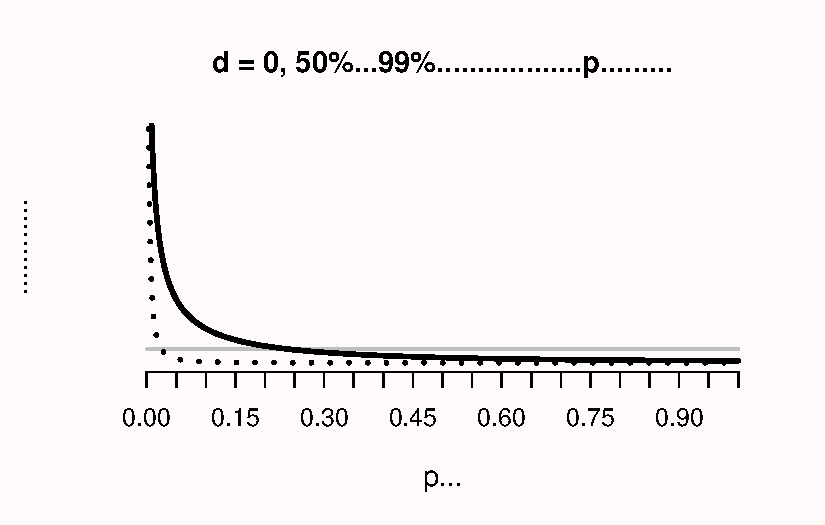
\includegraphics[width=1\textwidth,height=\textheight]{01-pvalue_files/figure-pdf/fig-paradox-1.pdf}

}

\caption{\label{fig-paradox}\emph{p}值分布(灰色水平线为0,50\%统计功效(黑色实线),99\%统计功效(黑色虚线))相比于\(H_1\)为真,当\(H_0\)为真时更可能出现\emph{p}略微小于0.05的值}

\end{figure}

\hypertarget{sec-correctlyinterpreting}{%
\section{\texorpdfstring{正确地解释和报告\emph{p}值}{正确地解释和报告p值}}\label{sec-correctlyinterpreting}}

虽然从严格的Neyman-Pearson方法的角度来看,报告\emph{p}\textless{}\(\alpha\)或\emph{p}\textgreater{}\(\alpha\)就足够了,但研究者还是应当报告确切的\emph{p}值。这便于后续再次分析结果时使用
(Appelbaum et al.,
2018),也便于并其他研究者将\emph{p}值与他们希望使用的\(\alpha\)水平进行比较
(Lehmann \& Romano,
2005)。因为所发表的结论是使用已知最大误差率的方式进行的,\emph{p}值永远不允许你肯定地陈述任何事情。即便我们把\(\alpha\)水平设定为0.000001,但任何一个结论都可能是错误的,Fisher
(1935)
提醒我们,即使是''百万分之一的几率''仍旧会发生,既不低于也不高于其某个恰当的概率,但只要发生在我们身上就是0和1的概率,纵使我们会非常惊讶为什么如此小的概率仍会发生在\emph{我们}身上''。这就是\textbf{重复研究}在科学领域很重要的原因。任何单一的发现都可能是一种侥幸,但如果几个重复的研究都能得到相同的结果,那么这种概率很快就会变得非常小。这种不确定性可能并没有反映在学术写作中,因为可以看到研究者会使用
``证明''、``显示''或
``已知''等字眼。在做完假设检验之后,有个稍长但更准确的说法是:

\begin{quote}
我们宣称了一个有或没有意义的效应,但也同时承认,如果学者们使用这种方法论提出结论,从长远来看,他们最多只有在\(\alpha\)\%或\(\beta\)\%上被误导,我们认为这是可以接受的。在不久的将来,除非出现新的数据或信息证明我们是错的,否则我们将假定这一结论是正确的。
\end{quote}

请记住,在Neyman-Pearson的理论框架下,研究者提出某种说法,但是这些说法\emph{不一定是真实的}。例如,OPERA合作组织在2011年报告说,他们所得到的观测数据似乎揭示了中微子的速度超过了光速。这一说法的第一错误率是百万分之0.2,\emph{假定错误纯粹是由随机误差造成的}。然而,实际上并没有研究者相信这一说法是真的,因为理论上中微子的运动速度不可能超过光速。事实上,后来发现是由于设备故障所导致的数据异常:一根光纤的连接不当,还有一个时钟振荡器的走的过快。然而,在提出这一说法的同时也公开邀请学界提供新的数据或信息,来证明这一说法有误。

当学者们在Neyman-Pearson统计推断方法下''接受''或''拒绝''一个假设时,他们并没有表明任何关于假设的信念或结论。相反,他们宣称自己是基于预设规则(即观察到的数据反映了世界的某种状态)的一种波普尔式\textbf{基本声明}。这些基本声明描绘的是已经进行的观察(例如,``我观察到了一只黑天鹅'')或已经发生的事件(例如,``接受间隔练习训练的学生,比不接受训练的学生在考试中表现得更好'')。

也就是说当下的某种声明与我们已经观测到的数据相关,但与我们用于预测的理论无关。某个声明与观测数据相关,因为它是一种统计推断,但它与理论无关,因为理论需要理论推断。数据永远无法``证明``一个理论是对还是错。一个基本声明可以\textbf{证实}一个从理论推导出来的预测,也可能无法证实。如果从一个理论中推导出的许多预测都得到了证实,我们就会越来越相信这个理论是接近真理的。这种理论的``接近真理性''叫做\textbf{逼真性}
(Niiniluoto, 1998; Popper,
2002)。报告假设检验时会出现的一个更短的声明是``p=.xx,即我们的预测在y\%的α水平下得到证实,或者``p=.xx,即我们所关注的效应量在对应的统计检验力下,预测没有被证实''。\(\alpha\)水平或者统计检验力往往只在文章的实验设计部分被提及,但是在结果部分重复他们能够提醒读者注意与你的声明相关的错误率。

甚至当我们做出正确的声明时,它的底层理论也可能是错误的。Popper (2002)
提醒我们``客观科学的实证基础并不是绝对的''。他争辩科学并不建立在坚固的基石之上,而是在沼泽中打下的木桩上,并指出``所以就目前而言,当确信桩的牢固程度足以承载结构后,我们就会停下来''。如Hacking
(1965)
写道:``拒绝不是反驳。多数拒绝只是试探性的''。所以当拒绝零模型时,我们是试探性的,并且知道有犯错的可能性,而不是一定要相信零模型是错的,以及我们用来进行预测的理论是对的。对Neyman
(1957)
而言,推断行为是一种``遵循当前实验结果,以一种特定方式去造就未来(直到被新的实验所迭代)的意志。所有的科学知识都是暂时的。

一些统计学家建议把p值解释成对证据的度量。例如,Bland (2015)
提出\emph{p}值可以被解释成一种对证据强度的``即粗略又完备''的指示,\emph{p}
\textgreater{} 0.1表示``很少或没有证据'',0.01 \textless{} \emph{p}
\textless{} 0.05表示``有证据'',\emph{p} \textless{}
0.001表示``证据很强''。从前面关于林德利悖论和\emph{p}值均匀分布的讨论中可以看出这是不正确的
(Johansson, 2011; Lakens,
2022)。如果你想量化证据,请看关于\protect\hyperlink{likelihoods}{似然性}或\protect\hyperlink{bayes}{贝叶斯统计}的章节。

\hypertarget{sec-misconceptions}{%
\section{\texorpdfstring{避免\emph{p}值的常见误解}{避免p值的常见误解}}\label{sec-misconceptions}}

\emph{p}值是在零假设为真的情况下,实际观测到的数据的概率或者临界值的概率。为了理解\emph{p值}能说明什么,我们尤其要注意\emph{p}值不能说明什么。首先,我们需要知道''零假设为真''是什么,以及当零假设为真时,数据的分布形态是怎样的。尽管零假设可以被设定为任意数值,在这里我们规定零假设就是均两组值差异为0。例如,在实验条件下和控制条件下计算两组因变量的差异。

区分零假设(假设在总体中平均值差异正好为0)和零模型(当零假设为真时,我们应该观察得到的数据模型)非常重要。零假设是一个位于0的点,而零模型则是一个分布。在教科书或者统计分析软件中,它门被可视化,可能会出现下面这样的图片。你可以看到,横轴代表\emph{t}值,并且临界值\emph{t}在1.96-2.00之间(取决于样本量)。之所以用\emph{t}值,是因为比较两组差异的统计检验是基于\emph{t}分布的,当实际得到的\emph{t}值大于临界值\emph{t}时,我们就认为\emph{p}值在统计上显著。

我个人认为,如果绘制的零模型是均值差的而非\emph{t}值的,解释起来会更加清楚。所以在下方,你会看见当比较样本量为50的两组数据时,均值差的零模型,假设它们的真实差异为0,两组的标准差均为1。因为它们的标准差为1,你也可以把均值差异解释为科恩\emph{d}效应量。所以,这也是样本量为50的样本在做独立样本\emph{t}检验,科恩\emph{d}为0时的分布。

\begin{verbatim}
Warning in title(...): conversion failure on 'N = 50 的零假设' in 'mbcsToSbcs':
dot substituted for <e7>
\end{verbatim}

\begin{verbatim}
Warning in title(...): conversion failure on 'N = 50 的零假设' in 'mbcsToSbcs':
dot substituted for <9a>
\end{verbatim}

\begin{verbatim}
Warning in title(...): conversion failure on 'N = 50 的零假设' in 'mbcsToSbcs':
dot substituted for <84>
\end{verbatim}

\begin{verbatim}
Warning in title(...): conversion failure on 'N = 50 的零假设' in 'mbcsToSbcs':
dot substituted for <e9>
\end{verbatim}

\begin{verbatim}
Warning in title(...): conversion failure on 'N = 50 的零假设' in 'mbcsToSbcs':
dot substituted for <9b>
\end{verbatim}

\begin{verbatim}
Warning in title(...): conversion failure on 'N = 50 的零假设' in 'mbcsToSbcs':
dot substituted for <b6>
\end{verbatim}

\begin{verbatim}
Warning in title(...): conversion failure on 'N = 50 的零假设' in 'mbcsToSbcs':
dot substituted for <e5>
\end{verbatim}

\begin{verbatim}
Warning in title(...): conversion failure on 'N = 50 的零假设' in 'mbcsToSbcs':
dot substituted for <81>
\end{verbatim}

\begin{verbatim}
Warning in title(...): conversion failure on 'N = 50 的零假设' in 'mbcsToSbcs':
dot substituted for <87>
\end{verbatim}

\begin{verbatim}
Warning in title(...): conversion failure on 'N = 50 的零假设' in 'mbcsToSbcs':
dot substituted for <e8>
\end{verbatim}

\begin{verbatim}
Warning in title(...): conversion failure on 'N = 50 的零假设' in 'mbcsToSbcs':
dot substituted for <ae>
\end{verbatim}

\begin{verbatim}
Warning in title(...): conversion failure on 'N = 50 的零假设' in 'mbcsToSbcs':
dot substituted for <be>
\end{verbatim}

\begin{verbatim}
Warning in title(...): conversion failure on '差异' in 'mbcsToSbcs': dot
substituted for <e5>
\end{verbatim}

\begin{verbatim}
Warning in title(...): conversion failure on '差异' in 'mbcsToSbcs': dot
substituted for <b7>
\end{verbatim}

\begin{verbatim}
Warning in title(...): conversion failure on '差异' in 'mbcsToSbcs': dot
substituted for <ae>
\end{verbatim}

\begin{verbatim}
Warning in title(...): conversion failure on '差异' in 'mbcsToSbcs': dot
substituted for <e5>
\end{verbatim}

\begin{verbatim}
Warning in title(...): conversion failure on '差异' in 'mbcsToSbcs': dot
substituted for <bc>
\end{verbatim}

\begin{verbatim}
Warning in title(...): conversion failure on '差异' in 'mbcsToSbcs': dot
substituted for <82>
\end{verbatim}

\begin{figure}

{\centering 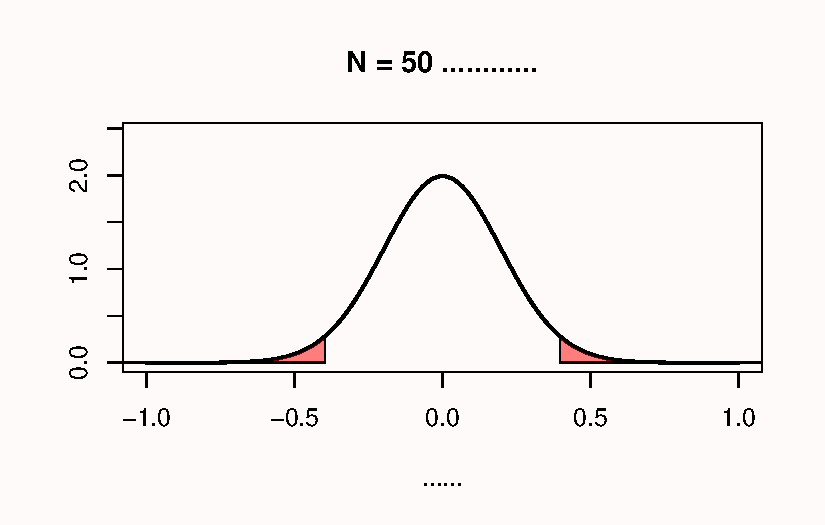
\includegraphics[width=1\textwidth,height=\textheight]{01-pvalue_files/figure-pdf/fig-fig131-1.pdf}

}

\caption{\label{fig-fig131}在每组收集50个观察值的独立样本t检验中,所得Cohen's
\emph{d}效应量的分布。}

\end{figure}

首先要注意到的是,我们期望的零模型的平均值是0。观察X轴,我们可以看到绘制的分布是以0为中心的。但是,即使总体的均值差是0,这也不意味着每个从总体中抽出的样本的均值差都为0。样本的值会围绕总体的值变化,是一个标准差和样本量的函数。

图中Y轴是概率密度,它代表的是连续分布中得到某一特定值的可能性。我们可以看到,最有可能得到的均值差是总体的真实值0,离0越远的值得到的可能性就越小。图中有两个区域标红了,这些区域代表分布的左尾部2.5\%的极端值,以及分布的右尾部2.5\%的极端值。它们共同构成了当真均值差恰好为0,样本量为50时,抽样分布的5\%的极端值的区域。当测量的值落在这个区域,相应的统计检验就认为两组在5\%的α水平上达到显著差异。换句话说,不超过5\%的均值差是离0足够远,会被认为是小概率事件的。因为零假设为真,如果测量得到这种小概率的平均值差异,即红色区域,则是犯了1型错误。

让我们假设上图中的零模型是正确的,并且我们测量得到两组之间的平均值差异为0.5。这种测量得到的差异落在分布右尾的红色区域。这意味着,在真实平均差值为0的假设下,测量得到的平均差值相是小概率事件。如果真实的平均差值为0,概率密度函数表明我们不应该测量得到平均差值为0.5。如果我们计算这个观测值的p值,它将低于5\%。观测到距离0远至0.5(当我们做双尾检验时,要么在均值的左边,要么在均值的右边)的平均差异的概率小于5\%。

我更喜欢用原始分数而不是t值来绘制零模型的另一个原因是,当样本量增加时,我们可以看到零模型是如何变化的。当我们收集5000个而不是50个观测值时,我们看到零模型仍然以0为中心------但在现在的零模型中,我们预计大多数值将非常接近0。

\begin{verbatim}
Warning in title(...): conversion failure on 'N = 5000的零假设' in
'mbcsToSbcs': dot substituted for <e7>
\end{verbatim}

\begin{verbatim}
Warning in title(...): conversion failure on 'N = 5000的零假设' in
'mbcsToSbcs': dot substituted for <9a>
\end{verbatim}

\begin{verbatim}
Warning in title(...): conversion failure on 'N = 5000的零假设' in
'mbcsToSbcs': dot substituted for <84>
\end{verbatim}

\begin{verbatim}
Warning in title(...): conversion failure on 'N = 5000的零假设' in
'mbcsToSbcs': dot substituted for <e9>
\end{verbatim}

\begin{verbatim}
Warning in title(...): conversion failure on 'N = 5000的零假设' in
'mbcsToSbcs': dot substituted for <9b>
\end{verbatim}

\begin{verbatim}
Warning in title(...): conversion failure on 'N = 5000的零假设' in
'mbcsToSbcs': dot substituted for <b6>
\end{verbatim}

\begin{verbatim}
Warning in title(...): conversion failure on 'N = 5000的零假设' in
'mbcsToSbcs': dot substituted for <e5>
\end{verbatim}

\begin{verbatim}
Warning in title(...): conversion failure on 'N = 5000的零假设' in
'mbcsToSbcs': dot substituted for <81>
\end{verbatim}

\begin{verbatim}
Warning in title(...): conversion failure on 'N = 5000的零假设' in
'mbcsToSbcs': dot substituted for <87>
\end{verbatim}

\begin{verbatim}
Warning in title(...): conversion failure on 'N = 5000的零假设' in
'mbcsToSbcs': dot substituted for <e8>
\end{verbatim}

\begin{verbatim}
Warning in title(...): conversion failure on 'N = 5000的零假设' in
'mbcsToSbcs': dot substituted for <ae>
\end{verbatim}

\begin{verbatim}
Warning in title(...): conversion failure on 'N = 5000的零假设' in
'mbcsToSbcs': dot substituted for <be>
\end{verbatim}

\begin{verbatim}
Warning in title(...): conversion failure on '差异' in 'mbcsToSbcs': dot
substituted for <e5>
\end{verbatim}

\begin{verbatim}
Warning in title(...): conversion failure on '差异' in 'mbcsToSbcs': dot
substituted for <b7>
\end{verbatim}

\begin{verbatim}
Warning in title(...): conversion failure on '差异' in 'mbcsToSbcs': dot
substituted for <ae>
\end{verbatim}

\begin{verbatim}
Warning in title(...): conversion failure on '差异' in 'mbcsToSbcs': dot
substituted for <e5>
\end{verbatim}

\begin{verbatim}
Warning in title(...): conversion failure on '差异' in 'mbcsToSbcs': dot
substituted for <bc>
\end{verbatim}

\begin{verbatim}
Warning in title(...): conversion failure on '差异' in 'mbcsToSbcs': dot
substituted for <82>
\end{verbatim}

\begin{figure}

{\centering 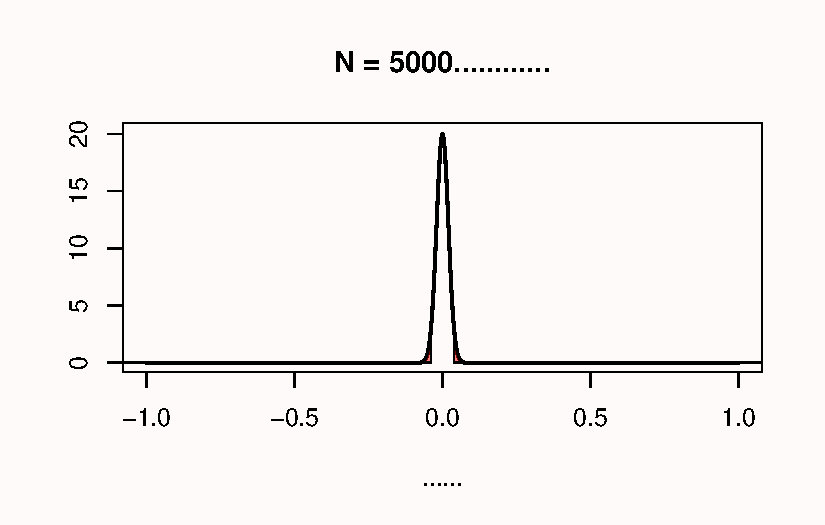
\includegraphics[width=1\textwidth,height=\textheight]{01-pvalue_files/figure-pdf/fig-fig132-1.pdf}

}

\caption{\label{fig-fig132}当d=0时,在每组收集5000个观察值的独立样本t检验中,所得Cohen's
\emph{d}效应量的分布。}

\end{figure}

由于均值差的分布是基于均值差的标准误,所以5000样本量的分布要窄得多。这个值是根据标准差和样本量计算的,如下所示:

\[\sqrt{\frac{\sigma_{1}^{2}}{n_{1}}+\frac{\sigma_{2}^{2}}{n_{2}}}\]
这个公式表明,均值差的标准误是每个组的标准差(σ)的平方除以该组的样本量,加在一起,然后取平方根。样本量越大,除以的数字就越大,因此均值差的标准误就越小。在n
=50的例子中,有标准差:

\[\sqrt{\frac{1^{2}}{50}+\frac{1^{2}}{50}}\] 因此,当n =
50时,两组均值差的标准误为0.2;当n =
5000时,均值差的标准误为0.02。假设抽样分布为正态分布,95\%的观测值落在1.96
个标准误之间。因此,对于样本量为50的样本,均值差应该在-1.96 * 0.2 =
-0.392和+1.96 * 0.2 = 0.392之间,我们可以看到,当n =
50时,红色区域大约从-0.392到0.392。对于样本量为5000的样本,均值差应在-1.96
* 0.02和+1.96 *
0.02之间,也就是说,应该介于-0.0392到0.0392之间。由于样本量较大(n =
5000),观测得到的均值差应该比较小样本(n=50)中观测得到的均值差更接近0.

如果我们抽出n =
5000的样本,并且观测到0.5的均值差,我们要清楚,这样的概率比起收集50个观测值发现0.5的均值差的要更小。我们现在几乎已经准备好介绍关于p值的常见误解,但在此之前,我们需要引入一个当零假设不为真时的数据模型。如果我们不是从一个真实均值差为0的模型中抽样,那么得到的备择模型会是什么样呢?一些软件
(比如 G*power, 见 图
Figure~\ref{fig-gpowerscreenshot})会同时显示出零模型(红色曲线)和备择模型(蓝色曲线):

\begin{figure}

{\centering 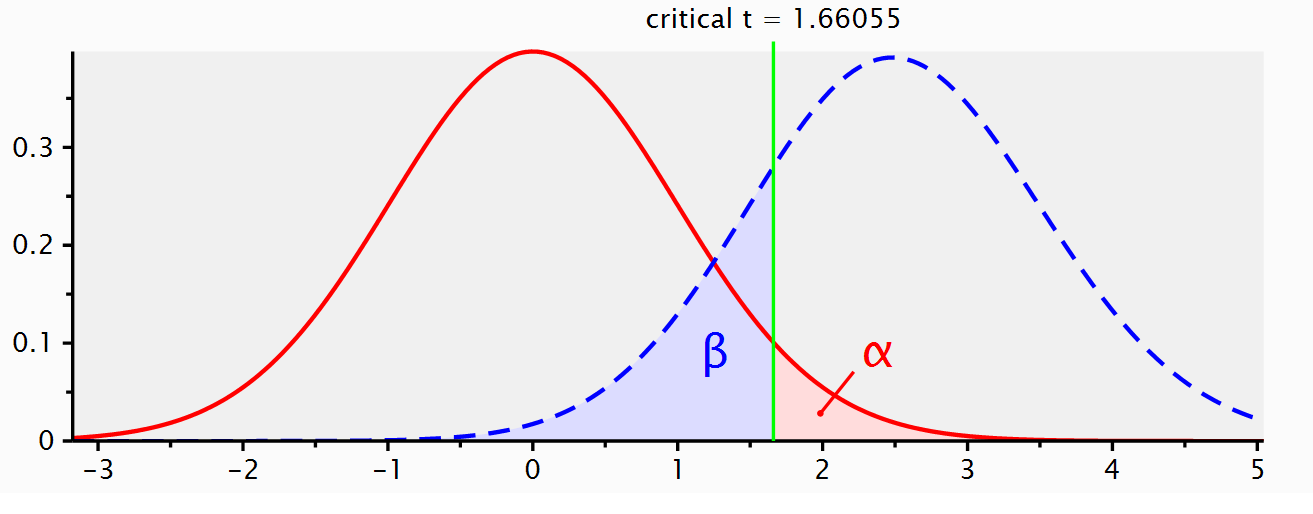
\includegraphics[width=1\textwidth,height=\textheight]{images/1.3.3.png}

}

\caption{\label{fig-gpowerscreenshot}G*Power软件截图显示了零模型(红色分布)和备择模型(蓝色分布)以及区分显著和非显著结果的临界\emph{t}值(1.66055)。}

\end{figure}

当我们做一项研究时,我们不知道真正的均值差是多少(如果我们已经知道了,为什么还要做这项研究?)但是,让我们假设有一个全知的存在,按照Paul
Meehl的说法,我们称呼祂为''无所不知的琼斯''。在我们从总体里收集50个观测值之前,``无所不知的琼斯''就已经知道了总体的真实均值差为0.5。那么在备择模型中,均差值就应该在0.5周围变化。下图显示了零假设成立时的数据模式(用灰线表示),和备择模型(用黑线表示),即假设总体中存在0.5的真实均值差的模型。

\begin{verbatim}
Warning in title(...): conversion failure on 'N = 50 的零假设和备择假设' in
'mbcsToSbcs': dot substituted for <e7>
\end{verbatim}

\begin{verbatim}
Warning in title(...): conversion failure on 'N = 50 的零假设和备择假设' in
'mbcsToSbcs': dot substituted for <9a>
\end{verbatim}

\begin{verbatim}
Warning in title(...): conversion failure on 'N = 50 的零假设和备择假设' in
'mbcsToSbcs': dot substituted for <84>
\end{verbatim}

\begin{verbatim}
Warning in title(...): conversion failure on 'N = 50 的零假设和备择假设' in
'mbcsToSbcs': dot substituted for <e9>
\end{verbatim}

\begin{verbatim}
Warning in title(...): conversion failure on 'N = 50 的零假设和备择假设' in
'mbcsToSbcs': dot substituted for <9b>
\end{verbatim}

\begin{verbatim}
Warning in title(...): conversion failure on 'N = 50 的零假设和备择假设' in
'mbcsToSbcs': dot substituted for <b6>
\end{verbatim}

\begin{verbatim}
Warning in title(...): conversion failure on 'N = 50 的零假设和备择假设' in
'mbcsToSbcs': dot substituted for <e5>
\end{verbatim}

\begin{verbatim}
Warning in title(...): conversion failure on 'N = 50 的零假设和备择假设' in
'mbcsToSbcs': dot substituted for <81>
\end{verbatim}

\begin{verbatim}
Warning in title(...): conversion failure on 'N = 50 的零假设和备择假设' in
'mbcsToSbcs': dot substituted for <87>
\end{verbatim}

\begin{verbatim}
Warning in title(...): conversion failure on 'N = 50 的零假设和备择假设' in
'mbcsToSbcs': dot substituted for <e8>
\end{verbatim}

\begin{verbatim}
Warning in title(...): conversion failure on 'N = 50 的零假设和备择假设' in
'mbcsToSbcs': dot substituted for <ae>
\end{verbatim}

\begin{verbatim}
Warning in title(...): conversion failure on 'N = 50 的零假设和备择假设' in
'mbcsToSbcs': dot substituted for <be>
\end{verbatim}

\begin{verbatim}
Warning in title(...): conversion failure on 'N = 50 的零假设和备择假设' in
'mbcsToSbcs': dot substituted for <e5>
\end{verbatim}

\begin{verbatim}
Warning in title(...): conversion failure on 'N = 50 的零假设和备择假设' in
'mbcsToSbcs': dot substituted for <92>
\end{verbatim}

\begin{verbatim}
Warning in title(...): conversion failure on 'N = 50 的零假设和备择假设' in
'mbcsToSbcs': dot substituted for <8c>
\end{verbatim}

\begin{verbatim}
Warning in title(...): conversion failure on 'N = 50 的零假设和备择假设' in
'mbcsToSbcs': dot substituted for <e5>
\end{verbatim}

\begin{verbatim}
Warning in title(...): conversion failure on 'N = 50 的零假设和备择假设' in
'mbcsToSbcs': dot substituted for <a4>
\end{verbatim}

\begin{verbatim}
Warning in title(...): conversion failure on 'N = 50 的零假设和备择假设' in
'mbcsToSbcs': dot substituted for <87>
\end{verbatim}

\begin{verbatim}
Warning in title(...): conversion failure on 'N = 50 的零假设和备择假设' in
'mbcsToSbcs': dot substituted for <e6>
\end{verbatim}

\begin{verbatim}
Warning in title(...): conversion failure on 'N = 50 的零假设和备择假设' in
'mbcsToSbcs': dot substituted for <8b>
\end{verbatim}

\begin{verbatim}
Warning in title(...): conversion failure on 'N = 50 的零假设和备择假设' in
'mbcsToSbcs': dot substituted for <a9>
\end{verbatim}

\begin{verbatim}
Warning in title(...): conversion failure on 'N = 50 的零假设和备择假设' in
'mbcsToSbcs': dot substituted for <e5>
\end{verbatim}

\begin{verbatim}
Warning in title(...): conversion failure on 'N = 50 的零假设和备择假设' in
'mbcsToSbcs': dot substituted for <81>
\end{verbatim}

\begin{verbatim}
Warning in title(...): conversion failure on 'N = 50 的零假设和备择假设' in
'mbcsToSbcs': dot substituted for <87>
\end{verbatim}

\begin{verbatim}
Warning in title(...): conversion failure on 'N = 50 的零假设和备择假设' in
'mbcsToSbcs': dot substituted for <e8>
\end{verbatim}

\begin{verbatim}
Warning in title(...): conversion failure on 'N = 50 的零假设和备择假设' in
'mbcsToSbcs': dot substituted for <ae>
\end{verbatim}

\begin{verbatim}
Warning in title(...): conversion failure on 'N = 50 的零假设和备择假设' in
'mbcsToSbcs': dot substituted for <be>
\end{verbatim}

\begin{verbatim}
Warning in title(...): conversion failure on '差异' in 'mbcsToSbcs': dot
substituted for <e5>
\end{verbatim}

\begin{verbatim}
Warning in title(...): conversion failure on '差异' in 'mbcsToSbcs': dot
substituted for <b7>
\end{verbatim}

\begin{verbatim}
Warning in title(...): conversion failure on '差异' in 'mbcsToSbcs': dot
substituted for <ae>
\end{verbatim}

\begin{verbatim}
Warning in title(...): conversion failure on '差异' in 'mbcsToSbcs': dot
substituted for <e5>
\end{verbatim}

\begin{verbatim}
Warning in title(...): conversion failure on '差异' in 'mbcsToSbcs': dot
substituted for <bc>
\end{verbatim}

\begin{verbatim}
Warning in title(...): conversion failure on '差异' in 'mbcsToSbcs': dot
substituted for <82>
\end{verbatim}

\begin{figure}

{\centering 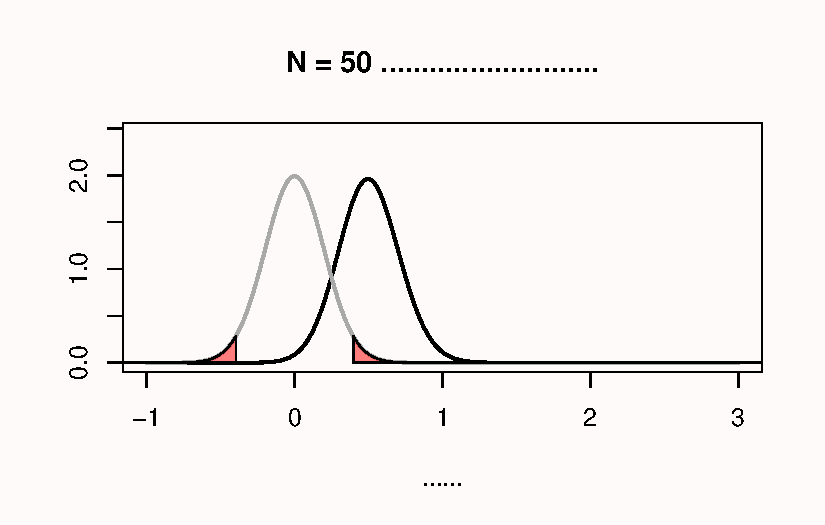
\includegraphics[width=1\textwidth,height=\textheight]{01-pvalue_files/figure-pdf/fig-fig134-1.pdf}

}

\caption{\label{fig-fig134}在\emph{d} =
0,每组收集50个观测值的独立样本\emph{t}检验中,Cohen's
\emph{d}效应量的分布。}

\end{figure}

但是''无所不知的琼斯''也可以说真实均值差是一个更大的值。假设在另一个研究中,在我们抽样之前,祂就说真实均值差是1.5。那么此时零假设模型不变,备择假设模型会向右移动。

您可以在此应用程序上在线调整备择模型和零模型:\url{http://shiny.ieis.tue.nl/d_p_power/}.
该应用程序允许你设定参加t检验的两组的样本量(从2到无穷大)、均值差(从0到2)和alpha水平。在图中,红色区域表示I类错误,蓝色区域表示II类错误(具体我们将在之后讨论)。该应用程序也会显示临界值:会有一条垂直线(样本量为50时,落在均值差为0.4处)和一句提示语------大于0.4代表效应显著。虽然没有提示语,我们应该知道此时小于-0.4也显著。这个应用程序也适用于双侧的独立t检验。

你可以看到,在表示临界均值差的竖线的左边有一个蓝色区域,它是备择模型的一部分。这就是犯II类错误的概率(或者代表1-统计力)。如果一个研究的统计力是80\%,代表我们能观测到的80\%的均值差都会落在代表临界值的那条线的右边。如果备择假设为真,但是我们又得到了小于临界值的效应,那么即使真的存在效应,此时的\emph{p}值应该大于0.05。你可以在应用程序中验证,当样本量越大,整个备择模型就越靠右,统计力也就越大。同时你也可以看到,样本量越大,分布越窄,低于临界值的分布越少(只要真实总体均值大于临界值)。最终,α水平越大,临界值代表的均值差越向左移,低于临界值的备择分布的面积就越小。

该应用程序还绘制了3个图,是不同α水平、不同样本量和不同真均值差下的功率曲线函数。用户可以在应用程序中调整这三个值,了解每个变量如何影响零模型和备择模型,看到达到统计水平上显著的均值差的大小和犯Ⅰ类以和Ⅱ类错误的概率。

到目前为止,零模型的几个方面应该已经变得逐渐清晰。首先,传统零假设中,总体均值差为0,但在你抽出的任何样本中,观测的均值差都落在一个以0为中心的分布中,通常会略大于或略小于0。其次,该分布的宽度取决于样本量和标准差。研究的样本量越大,分布就越集中于0。最后,当观测到的均值差落在零模型尾端时,结果被认为是出人意料的。离0越远,这个结果就越令人惊讶。但是,当零模型为真时,这些令人惊讶的结果发生的概率为α水平(也被称为Ⅰ类错误)。请记住,当研究人员得出总体存在差异时,但实际的均值差为0时,就会发生第一类错误。

我们现在终于准备好可以厘清一些关于\emph{p}值的常见误解了。让我们来回顾一下科学文献中报告过的一系列常见误解。其中一些也许听起来只是语言表达问题。乍一看,人们很容易认为这句话传达了正确的想法,即使在书面形式上并不正确。然而,当一个陈述在形式上不正确时,它就是错误的。正是因为人们会经常误解\emph{p}值,所以在形式上正确解释\emph{p}值是非常重要的。

\hypertarget{sec-misconception1}{%
\subsection{\texorpdfstring{误解
1:\emph{p}值不显著意味着零假设为真。}{误解 1:p值不显著意味着零假设为真。}}\label{sec-misconception1}}

此误解的一个常见版本体现在句子'因为\emph{p} \textgreater{} 0.05,
我们可以推断效应不存在'中;这句话也可以是'差异不存在(\emph{p}
\textgreater{} 0.05)'。

在谈论细节之前,我想提醒你一个简单的事实,它会使你辨明许多关于\emph{p}值的误解:p值是有关数据概率的解释,而非一个假设或理论的概率的解释。不论何时你看到\emph{p}值被用于解释一个假设或理论的概率,你就知道事情有些不太对。有关假设的例子有:`零假设为真'或'备择假设为真',它们都是指零模型或者备择模型为真的概率是100\%。更微妙的表述有'观测到的差异不是出于偶然'。当零假设为真时,观测到的差异只是'由于偶然'(而不是由于真实差异的存在),与之前一样,这句话是指零假设100\%为真。

当你得出'效应不存在'或者'不存在差异'的结论时,你也就是在说零假设100\%为真。但是由于\emph{p}值是有关数据概率的解释,你应该避免仅基于\emph{p}值去解释理论存在的概率。\emph{p}值的设计是用来帮助你识别嘈杂的数据生成(即真实情况)中意料之外的结果。它并不能量化一个假设为真的概率。

让我们举一个具体的例子来说明为什么不显著的结果并不意味着零假设就是正确的。在下图中,无所不知的琼斯告诉我们,真均值差为0.5。我们可以从图中看出,当备择假设为真时,期望的均值差的可视化分布以0.5为中心。我们观测到的均值差是0.35。这个值还没有极端到足以在统计学上与0有显著差异。同样从图中可以看出,这个值没有落在零模型的红色区域(因此,\emph{p}值并不小于我们规定的α水平)。

然而,鉴于真均值差是0.5,观测均值差为0.35不光很可能发生,更可能是在备择模型而非是零模型上观测到。你可以看到这一点,因为在零模型中,均值差为0.35的概率密度曲线的高度约为0.5,在备择模型中概率密度曲线的高度则接近1.5。详情请参见\protect\hyperlink{likettest}{可能性}一章。

\begin{verbatim}
Warning in title(...): conversion failure on 'N = 50 的零假设和备择假设' in
'mbcsToSbcs': dot substituted for <e7>
\end{verbatim}

\begin{verbatim}
Warning in title(...): conversion failure on 'N = 50 的零假设和备择假设' in
'mbcsToSbcs': dot substituted for <9a>
\end{verbatim}

\begin{verbatim}
Warning in title(...): conversion failure on 'N = 50 的零假设和备择假设' in
'mbcsToSbcs': dot substituted for <84>
\end{verbatim}

\begin{verbatim}
Warning in title(...): conversion failure on 'N = 50 的零假设和备择假设' in
'mbcsToSbcs': dot substituted for <e9>
\end{verbatim}

\begin{verbatim}
Warning in title(...): conversion failure on 'N = 50 的零假设和备择假设' in
'mbcsToSbcs': dot substituted for <9b>
\end{verbatim}

\begin{verbatim}
Warning in title(...): conversion failure on 'N = 50 的零假设和备择假设' in
'mbcsToSbcs': dot substituted for <b6>
\end{verbatim}

\begin{verbatim}
Warning in title(...): conversion failure on 'N = 50 的零假设和备择假设' in
'mbcsToSbcs': dot substituted for <e5>
\end{verbatim}

\begin{verbatim}
Warning in title(...): conversion failure on 'N = 50 的零假设和备择假设' in
'mbcsToSbcs': dot substituted for <81>
\end{verbatim}

\begin{verbatim}
Warning in title(...): conversion failure on 'N = 50 的零假设和备择假设' in
'mbcsToSbcs': dot substituted for <87>
\end{verbatim}

\begin{verbatim}
Warning in title(...): conversion failure on 'N = 50 的零假设和备择假设' in
'mbcsToSbcs': dot substituted for <e8>
\end{verbatim}

\begin{verbatim}
Warning in title(...): conversion failure on 'N = 50 的零假设和备择假设' in
'mbcsToSbcs': dot substituted for <ae>
\end{verbatim}

\begin{verbatim}
Warning in title(...): conversion failure on 'N = 50 的零假设和备择假设' in
'mbcsToSbcs': dot substituted for <be>
\end{verbatim}

\begin{verbatim}
Warning in title(...): conversion failure on 'N = 50 的零假设和备择假设' in
'mbcsToSbcs': dot substituted for <e5>
\end{verbatim}

\begin{verbatim}
Warning in title(...): conversion failure on 'N = 50 的零假设和备择假设' in
'mbcsToSbcs': dot substituted for <92>
\end{verbatim}

\begin{verbatim}
Warning in title(...): conversion failure on 'N = 50 的零假设和备择假设' in
'mbcsToSbcs': dot substituted for <8c>
\end{verbatim}

\begin{verbatim}
Warning in title(...): conversion failure on 'N = 50 的零假设和备择假设' in
'mbcsToSbcs': dot substituted for <e5>
\end{verbatim}

\begin{verbatim}
Warning in title(...): conversion failure on 'N = 50 的零假设和备择假设' in
'mbcsToSbcs': dot substituted for <a4>
\end{verbatim}

\begin{verbatim}
Warning in title(...): conversion failure on 'N = 50 的零假设和备择假设' in
'mbcsToSbcs': dot substituted for <87>
\end{verbatim}

\begin{verbatim}
Warning in title(...): conversion failure on 'N = 50 的零假设和备择假设' in
'mbcsToSbcs': dot substituted for <e6>
\end{verbatim}

\begin{verbatim}
Warning in title(...): conversion failure on 'N = 50 的零假设和备择假设' in
'mbcsToSbcs': dot substituted for <8b>
\end{verbatim}

\begin{verbatim}
Warning in title(...): conversion failure on 'N = 50 的零假设和备择假设' in
'mbcsToSbcs': dot substituted for <a9>
\end{verbatim}

\begin{verbatim}
Warning in title(...): conversion failure on 'N = 50 的零假设和备择假设' in
'mbcsToSbcs': dot substituted for <e5>
\end{verbatim}

\begin{verbatim}
Warning in title(...): conversion failure on 'N = 50 的零假设和备择假设' in
'mbcsToSbcs': dot substituted for <81>
\end{verbatim}

\begin{verbatim}
Warning in title(...): conversion failure on 'N = 50 的零假设和备择假设' in
'mbcsToSbcs': dot substituted for <87>
\end{verbatim}

\begin{verbatim}
Warning in title(...): conversion failure on 'N = 50 的零假设和备择假设' in
'mbcsToSbcs': dot substituted for <e8>
\end{verbatim}

\begin{verbatim}
Warning in title(...): conversion failure on 'N = 50 的零假设和备择假设' in
'mbcsToSbcs': dot substituted for <ae>
\end{verbatim}

\begin{verbatim}
Warning in title(...): conversion failure on 'N = 50 的零假设和备择假设' in
'mbcsToSbcs': dot substituted for <be>
\end{verbatim}

\begin{verbatim}
Warning in title(...): conversion failure on '差异' in 'mbcsToSbcs': dot
substituted for <e5>
\end{verbatim}

\begin{verbatim}
Warning in title(...): conversion failure on '差异' in 'mbcsToSbcs': dot
substituted for <b7>
\end{verbatim}

\begin{verbatim}
Warning in title(...): conversion failure on '差异' in 'mbcsToSbcs': dot
substituted for <ae>
\end{verbatim}

\begin{verbatim}
Warning in title(...): conversion failure on '差异' in 'mbcsToSbcs': dot
substituted for <e5>
\end{verbatim}

\begin{verbatim}
Warning in title(...): conversion failure on '差异' in 'mbcsToSbcs': dot
substituted for <bc>
\end{verbatim}

\begin{verbatim}
Warning in title(...): conversion failure on '差异' in 'mbcsToSbcs': dot
substituted for <82>
\end{verbatim}

\begin{verbatim}
Warning in text.default(0.35, 2.4, paste("所得均值差异"), cex = 1): conversion
failure on '所得均值差异' in 'mbcsToSbcs': dot substituted for <e6>
\end{verbatim}

\begin{verbatim}
Warning in text.default(0.35, 2.4, paste("所得均值差异"), cex = 1): conversion
failure on '所得均值差异' in 'mbcsToSbcs': dot substituted for <89>
\end{verbatim}

\begin{verbatim}
Warning in text.default(0.35, 2.4, paste("所得均值差异"), cex = 1): conversion
failure on '所得均值差异' in 'mbcsToSbcs': dot substituted for <80>
\end{verbatim}

\begin{verbatim}
Warning in text.default(0.35, 2.4, paste("所得均值差异"), cex = 1): conversion
failure on '所得均值差异' in 'mbcsToSbcs': dot substituted for <e5>
\end{verbatim}

\begin{verbatim}
Warning in text.default(0.35, 2.4, paste("所得均值差异"), cex = 1): conversion
failure on '所得均值差异' in 'mbcsToSbcs': dot substituted for <be>
\end{verbatim}

\begin{verbatim}
Warning in text.default(0.35, 2.4, paste("所得均值差异"), cex = 1): conversion
failure on '所得均值差异' in 'mbcsToSbcs': dot substituted for <97>
\end{verbatim}

\begin{verbatim}
Warning in text.default(0.35, 2.4, paste("所得均值差异"), cex = 1): conversion
failure on '所得均值差异' in 'mbcsToSbcs': dot substituted for <e5>
\end{verbatim}

\begin{verbatim}
Warning in text.default(0.35, 2.4, paste("所得均值差异"), cex = 1): conversion
failure on '所得均值差异' in 'mbcsToSbcs': dot substituted for <9d>
\end{verbatim}

\begin{verbatim}
Warning in text.default(0.35, 2.4, paste("所得均值差异"), cex = 1): conversion
failure on '所得均值差异' in 'mbcsToSbcs': dot substituted for <87>
\end{verbatim}

\begin{verbatim}
Warning in text.default(0.35, 2.4, paste("所得均值差异"), cex = 1): conversion
failure on '所得均值差异' in 'mbcsToSbcs': dot substituted for <e5>
\end{verbatim}

\begin{verbatim}
Warning in text.default(0.35, 2.4, paste("所得均值差异"), cex = 1): conversion
failure on '所得均值差异' in 'mbcsToSbcs': dot substituted for <80>
\end{verbatim}

\begin{verbatim}
Warning in text.default(0.35, 2.4, paste("所得均值差异"), cex = 1): conversion
failure on '所得均值差异' in 'mbcsToSbcs': dot substituted for <bc>
\end{verbatim}

\begin{verbatim}
Warning in text.default(0.35, 2.4, paste("所得均值差异"), cex = 1): conversion
failure on '所得均值差异' in 'mbcsToSbcs': dot substituted for <e5>
\end{verbatim}

\begin{verbatim}
Warning in text.default(0.35, 2.4, paste("所得均值差异"), cex = 1): conversion
failure on '所得均值差异' in 'mbcsToSbcs': dot substituted for <b7>
\end{verbatim}

\begin{verbatim}
Warning in text.default(0.35, 2.4, paste("所得均值差异"), cex = 1): conversion
failure on '所得均值差异' in 'mbcsToSbcs': dot substituted for <ae>
\end{verbatim}

\begin{verbatim}
Warning in text.default(0.35, 2.4, paste("所得均值差异"), cex = 1): conversion
failure on '所得均值差异' in 'mbcsToSbcs': dot substituted for <e5>
\end{verbatim}

\begin{verbatim}
Warning in text.default(0.35, 2.4, paste("所得均值差异"), cex = 1): conversion
failure on '所得均值差异' in 'mbcsToSbcs': dot substituted for <bc>
\end{verbatim}

\begin{verbatim}
Warning in text.default(0.35, 2.4, paste("所得均值差异"), cex = 1): conversion
failure on '所得均值差异' in 'mbcsToSbcs': dot substituted for <82>
\end{verbatim}

\begin{verbatim}
Warning in text.default(0.35, 2.4, paste("所得均值差异"), cex = 1): font
metrics unknown for Unicode character U+6240
\end{verbatim}

\begin{verbatim}
Warning in text.default(0.35, 2.4, paste("所得均值差异"), cex = 1): font
metrics unknown for Unicode character U+5f97
\end{verbatim}

\begin{verbatim}
Warning in text.default(0.35, 2.4, paste("所得均值差异"), cex = 1): font
metrics unknown for Unicode character U+5747
\end{verbatim}

\begin{verbatim}
Warning in text.default(0.35, 2.4, paste("所得均值差异"), cex = 1): font
metrics unknown for Unicode character U+503c
\end{verbatim}

\begin{verbatim}
Warning in text.default(0.35, 2.4, paste("所得均值差异"), cex = 1): font
metrics unknown for Unicode character U+5dee
\end{verbatim}

\begin{verbatim}
Warning in text.default(0.35, 2.4, paste("所得均值差异"), cex = 1): font
metrics unknown for Unicode character U+5f02
\end{verbatim}

\begin{figure}

{\centering 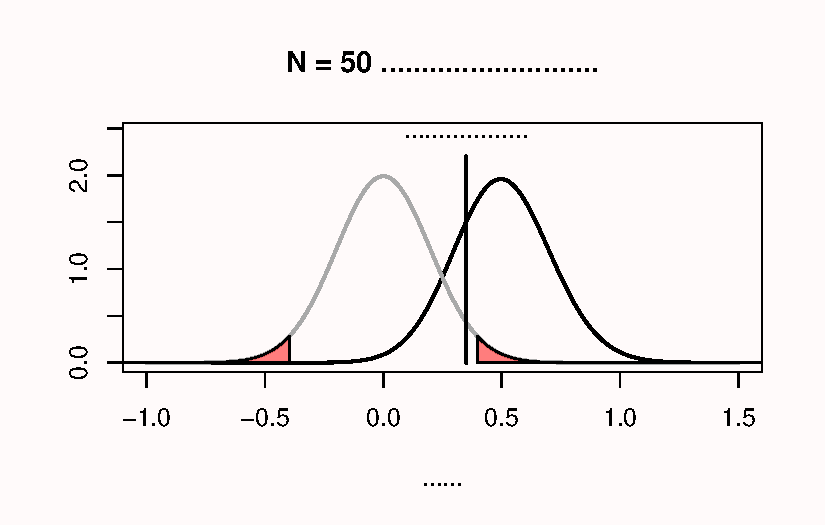
\includegraphics[width=1\textwidth,height=\textheight]{01-pvalue_files/figure-pdf/fig-fig136-1.pdf}

}

\caption{\label{fig-fig136}在\emph{d} = 0.35时,对\emph{d} = 0和\emph{d}
= 0.5进行每组50个观测值的独立样本t检验,所得Cohen's
\emph{d}效应量的分布。}

\end{figure}

如果我们假定零假设为真,所有的p值都告诉我们均值差为0.35并不是非常出人意料。这可能有很多原因。在真实世界中,并不存在无所不知的琼斯告诉我们真均值差,就像上图所示,有可能存在一个真实效应。

那么我们应该怎么陈述呢?解决方案很微妙,但也很重要。让我们再看看之前做的两个错误陈述的例子。首先,``因为\emph{p}
\textgreater{}
0.05,我们可以推断效应不存在''这个陈述是错误的,因为很有可能效应是存在的(请记住\emph{p}值是有关数据的解释而不是有效应或无效应的概率)。
费希尔对于p值的解释是我们可以得出一个小概率事件的发生或者零假设是错误的(他的原话是:``要么是发生了及其罕见的事件,要么是随机分布的原假设不正确'')。这可能听起来像是有关理论的概率的解释,但实际只是在p值很小时,对两种可能出现的场景的陈述(你犯Ⅰ型错误或者备择假设才为真)。真阳性和假阳性都是可能的,并且我们不量化两种可能性出现的概率(例如,并不是说零假设为真的概率是95\%)。从内曼-皮尔逊的角度,p
\textgreater{}
.05意味着我们不能拒绝零假设,因为我们有着5\%以下的预期错误率。

如果你对于推断效应缺失感兴趣,零假设检验不是你需要的工具。零假设检验回答的问题是'在期望的错误率下,我可以拒绝零假设吗?'。当\emph{p}
\textgreater{}
0.05,你不能拒绝零假设时,零假设是真还是假是不能仅仅基于\emph{p}值得出的(就像'无'的概念:既不是真也不是假)。幸运地是,已经开发了别的统计方法来回答效应缺失的问题,例如
\protect\hyperlink{equivalencetest}{等效检验}, 贝叶斯因子和贝叶斯估计
(请参见 Harms \& Lakens (2018), 了解概述).

第二个不正确的说法是'没有差异'。这个陈述改正起来要容易些。你可以写'没有统计学上的显著差异'。当然,两者有点重复,因为你基本上在用两种不同的方式说\emph{p}值大于α水平,但至少这个说法在形式上是正确的。`没有差异'和'没有统计学上的显著差异'可能听起来差不多,但前者你实际上在说'差异为0',而后者你是在说'差异不足以使\emph{p}
\textless{}
.05'。虽然我从未见过有人这样做,但是更完整的说法应该是'鉴于样本量是每组50,α水平是0.05,观测差异只有大于0.4才能达到统计学上的显著,由于我们观测的差异是0.35,因此我们不能拒绝零假设'。如果这看起来不是一个令人满意的结论,请记住,零假设检验的设计不是为了得出效应缺失的有趣结论------你需要了解等效检验,来得到有关零效应更令人满意的答案。

\hypertarget{ux8befux89e3-2pux503cux663eux8457ux610fux5473ux7740ux96f6ux5047ux8bbeux4e3aux5047}{%
\subsection{\texorpdfstring{误解
2:\emph{p}值显著意味着零假设为假。}{误解 2:p值显著意味着零假设为假。}}\label{ux8befux89e3-2pux503cux663eux8457ux610fux5473ux7740ux96f6ux5047ux8bbeux4e3aux5047}}

这是上一个误解的另一面。基于这种误解的错误陈述有'\emph{p} \textless{}
.05,因此效应存在',或'两组之间存在差异,\emph{p} \textless{}
.05'。像之前一样,这些陈述都是在暗指零假设为假的概率是100\%,备择假设才为真。

举一个简单的例子,说明为什么这些极端的语句是不正确的。假设我们使用下面的命令在R中生成一系列数字:

\begin{Shaded}
\begin{Highlighting}[]
\FunctionTok{rnorm}\NormalTok{(}\AttributeTok{n =} \DecValTok{50}\NormalTok{, }\AttributeTok{mean =} \DecValTok{0}\NormalTok{, }\AttributeTok{sd =} \DecValTok{1}\NormalTok{)}
\end{Highlighting}
\end{Shaded}

\begin{verbatim}
 [1]  0.163513992 -0.139051542 -1.284396973  0.397820532  1.415852026
 [6] -1.617861560  0.344050012 -0.451496175  1.258463136 -1.056491773
[11] -0.264032641  1.084720555  0.594974986  1.623746490 -0.433084998
[16] -1.194687687 -0.482815946 -1.715865089  0.317943102  0.275290657
[21]  0.539318562 -0.503650594  0.282980761  1.483571943 -0.272680730
[26]  0.315058705 -0.331452728  0.007979148  0.980443139  2.063931654
[31] -0.264805948 -0.090789793 -1.125752719 -1.281248315  1.042082177
[36] -0.607326283 -1.303144112  1.132740344 -0.335216795 -1.042496195
[41]  1.880986644  0.183789709  0.713560552  0.947490154  0.065580965
[46]  0.389474876  0.850295804 -0.421465812  0.188445230  0.985323765
\end{verbatim}

该命令会从一个平均值为0、标准差为1的分布中随机生成50个观察值(从长远来看------生成的每个样本的平均值和标准差都会有所不同)。想象我们运行这个命令一次,得到一个平均值为0.5的分布。下面的图画出了这个分布。假设我们可以做它和0的单样本t检验,得到\emph{p}
\textless{}
.05,此检验告诉我们,我们观测到的数据与0有显著差异,但此时R函数中随机数生成器依然按照原来的指令运行,生成的数据的真实均值为0。

\begin{verbatim}
Warning in title(...): conversion failure on 'N = 50 的零假设和备择假设' in
'mbcsToSbcs': dot substituted for <e7>
\end{verbatim}

\begin{verbatim}
Warning in title(...): conversion failure on 'N = 50 的零假设和备择假设' in
'mbcsToSbcs': dot substituted for <9a>
\end{verbatim}

\begin{verbatim}
Warning in title(...): conversion failure on 'N = 50 的零假设和备择假设' in
'mbcsToSbcs': dot substituted for <84>
\end{verbatim}

\begin{verbatim}
Warning in title(...): conversion failure on 'N = 50 的零假设和备择假设' in
'mbcsToSbcs': dot substituted for <e9>
\end{verbatim}

\begin{verbatim}
Warning in title(...): conversion failure on 'N = 50 的零假设和备择假设' in
'mbcsToSbcs': dot substituted for <9b>
\end{verbatim}

\begin{verbatim}
Warning in title(...): conversion failure on 'N = 50 的零假设和备择假设' in
'mbcsToSbcs': dot substituted for <b6>
\end{verbatim}

\begin{verbatim}
Warning in title(...): conversion failure on 'N = 50 的零假设和备择假设' in
'mbcsToSbcs': dot substituted for <e5>
\end{verbatim}

\begin{verbatim}
Warning in title(...): conversion failure on 'N = 50 的零假设和备择假设' in
'mbcsToSbcs': dot substituted for <81>
\end{verbatim}

\begin{verbatim}
Warning in title(...): conversion failure on 'N = 50 的零假设和备择假设' in
'mbcsToSbcs': dot substituted for <87>
\end{verbatim}

\begin{verbatim}
Warning in title(...): conversion failure on 'N = 50 的零假设和备择假设' in
'mbcsToSbcs': dot substituted for <e8>
\end{verbatim}

\begin{verbatim}
Warning in title(...): conversion failure on 'N = 50 的零假设和备择假设' in
'mbcsToSbcs': dot substituted for <ae>
\end{verbatim}

\begin{verbatim}
Warning in title(...): conversion failure on 'N = 50 的零假设和备择假设' in
'mbcsToSbcs': dot substituted for <be>
\end{verbatim}

\begin{verbatim}
Warning in title(...): conversion failure on 'N = 50 的零假设和备择假设' in
'mbcsToSbcs': dot substituted for <e5>
\end{verbatim}

\begin{verbatim}
Warning in title(...): conversion failure on 'N = 50 的零假设和备择假设' in
'mbcsToSbcs': dot substituted for <92>
\end{verbatim}

\begin{verbatim}
Warning in title(...): conversion failure on 'N = 50 的零假设和备择假设' in
'mbcsToSbcs': dot substituted for <8c>
\end{verbatim}

\begin{verbatim}
Warning in title(...): conversion failure on 'N = 50 的零假设和备择假设' in
'mbcsToSbcs': dot substituted for <e5>
\end{verbatim}

\begin{verbatim}
Warning in title(...): conversion failure on 'N = 50 的零假设和备择假设' in
'mbcsToSbcs': dot substituted for <a4>
\end{verbatim}

\begin{verbatim}
Warning in title(...): conversion failure on 'N = 50 的零假设和备择假设' in
'mbcsToSbcs': dot substituted for <87>
\end{verbatim}

\begin{verbatim}
Warning in title(...): conversion failure on 'N = 50 的零假设和备择假设' in
'mbcsToSbcs': dot substituted for <e6>
\end{verbatim}

\begin{verbatim}
Warning in title(...): conversion failure on 'N = 50 的零假设和备择假设' in
'mbcsToSbcs': dot substituted for <8b>
\end{verbatim}

\begin{verbatim}
Warning in title(...): conversion failure on 'N = 50 的零假设和备择假设' in
'mbcsToSbcs': dot substituted for <a9>
\end{verbatim}

\begin{verbatim}
Warning in title(...): conversion failure on 'N = 50 的零假设和备择假设' in
'mbcsToSbcs': dot substituted for <e5>
\end{verbatim}

\begin{verbatim}
Warning in title(...): conversion failure on 'N = 50 的零假设和备择假设' in
'mbcsToSbcs': dot substituted for <81>
\end{verbatim}

\begin{verbatim}
Warning in title(...): conversion failure on 'N = 50 的零假设和备择假设' in
'mbcsToSbcs': dot substituted for <87>
\end{verbatim}

\begin{verbatim}
Warning in title(...): conversion failure on 'N = 50 的零假设和备择假设' in
'mbcsToSbcs': dot substituted for <e8>
\end{verbatim}

\begin{verbatim}
Warning in title(...): conversion failure on 'N = 50 的零假设和备择假设' in
'mbcsToSbcs': dot substituted for <ae>
\end{verbatim}

\begin{verbatim}
Warning in title(...): conversion failure on 'N = 50 的零假设和备择假设' in
'mbcsToSbcs': dot substituted for <be>
\end{verbatim}

\begin{verbatim}
Warning in title(...): conversion failure on '差异' in 'mbcsToSbcs': dot
substituted for <e5>
\end{verbatim}

\begin{verbatim}
Warning in title(...): conversion failure on '差异' in 'mbcsToSbcs': dot
substituted for <b7>
\end{verbatim}

\begin{verbatim}
Warning in title(...): conversion failure on '差异' in 'mbcsToSbcs': dot
substituted for <ae>
\end{verbatim}

\begin{verbatim}
Warning in title(...): conversion failure on '差异' in 'mbcsToSbcs': dot
substituted for <e5>
\end{verbatim}

\begin{verbatim}
Warning in title(...): conversion failure on '差异' in 'mbcsToSbcs': dot
substituted for <bc>
\end{verbatim}

\begin{verbatim}
Warning in title(...): conversion failure on '差异' in 'mbcsToSbcs': dot
substituted for <82>
\end{verbatim}

\begin{verbatim}
Warning in text.default(0.5, 2.4, paste("所得均值差异"), cex = 1): conversion
failure on '所得均值差异' in 'mbcsToSbcs': dot substituted for <e6>
\end{verbatim}

\begin{verbatim}
Warning in text.default(0.5, 2.4, paste("所得均值差异"), cex = 1): conversion
failure on '所得均值差异' in 'mbcsToSbcs': dot substituted for <89>
\end{verbatim}

\begin{verbatim}
Warning in text.default(0.5, 2.4, paste("所得均值差异"), cex = 1): conversion
failure on '所得均值差异' in 'mbcsToSbcs': dot substituted for <80>
\end{verbatim}

\begin{verbatim}
Warning in text.default(0.5, 2.4, paste("所得均值差异"), cex = 1): conversion
failure on '所得均值差异' in 'mbcsToSbcs': dot substituted for <e5>
\end{verbatim}

\begin{verbatim}
Warning in text.default(0.5, 2.4, paste("所得均值差异"), cex = 1): conversion
failure on '所得均值差异' in 'mbcsToSbcs': dot substituted for <be>
\end{verbatim}

\begin{verbatim}
Warning in text.default(0.5, 2.4, paste("所得均值差异"), cex = 1): conversion
failure on '所得均值差异' in 'mbcsToSbcs': dot substituted for <97>
\end{verbatim}

\begin{verbatim}
Warning in text.default(0.5, 2.4, paste("所得均值差异"), cex = 1): conversion
failure on '所得均值差异' in 'mbcsToSbcs': dot substituted for <e5>
\end{verbatim}

\begin{verbatim}
Warning in text.default(0.5, 2.4, paste("所得均值差异"), cex = 1): conversion
failure on '所得均值差异' in 'mbcsToSbcs': dot substituted for <9d>
\end{verbatim}

\begin{verbatim}
Warning in text.default(0.5, 2.4, paste("所得均值差异"), cex = 1): conversion
failure on '所得均值差异' in 'mbcsToSbcs': dot substituted for <87>
\end{verbatim}

\begin{verbatim}
Warning in text.default(0.5, 2.4, paste("所得均值差异"), cex = 1): conversion
failure on '所得均值差异' in 'mbcsToSbcs': dot substituted for <e5>
\end{verbatim}

\begin{verbatim}
Warning in text.default(0.5, 2.4, paste("所得均值差异"), cex = 1): conversion
failure on '所得均值差异' in 'mbcsToSbcs': dot substituted for <80>
\end{verbatim}

\begin{verbatim}
Warning in text.default(0.5, 2.4, paste("所得均值差异"), cex = 1): conversion
failure on '所得均值差异' in 'mbcsToSbcs': dot substituted for <bc>
\end{verbatim}

\begin{verbatim}
Warning in text.default(0.5, 2.4, paste("所得均值差异"), cex = 1): conversion
failure on '所得均值差异' in 'mbcsToSbcs': dot substituted for <e5>
\end{verbatim}

\begin{verbatim}
Warning in text.default(0.5, 2.4, paste("所得均值差异"), cex = 1): conversion
failure on '所得均值差异' in 'mbcsToSbcs': dot substituted for <b7>
\end{verbatim}

\begin{verbatim}
Warning in text.default(0.5, 2.4, paste("所得均值差异"), cex = 1): conversion
failure on '所得均值差异' in 'mbcsToSbcs': dot substituted for <ae>
\end{verbatim}

\begin{verbatim}
Warning in text.default(0.5, 2.4, paste("所得均值差异"), cex = 1): conversion
failure on '所得均值差异' in 'mbcsToSbcs': dot substituted for <e5>
\end{verbatim}

\begin{verbatim}
Warning in text.default(0.5, 2.4, paste("所得均值差异"), cex = 1): conversion
failure on '所得均值差异' in 'mbcsToSbcs': dot substituted for <bc>
\end{verbatim}

\begin{verbatim}
Warning in text.default(0.5, 2.4, paste("所得均值差异"), cex = 1): conversion
failure on '所得均值差异' in 'mbcsToSbcs': dot substituted for <82>
\end{verbatim}

\begin{verbatim}
Warning in text.default(0.5, 2.4, paste("所得均值差异"), cex = 1): font metrics
unknown for Unicode character U+6240
\end{verbatim}

\begin{verbatim}
Warning in text.default(0.5, 2.4, paste("所得均值差异"), cex = 1): font metrics
unknown for Unicode character U+5f97
\end{verbatim}

\begin{verbatim}
Warning in text.default(0.5, 2.4, paste("所得均值差异"), cex = 1): font metrics
unknown for Unicode character U+5747
\end{verbatim}

\begin{verbatim}
Warning in text.default(0.5, 2.4, paste("所得均值差异"), cex = 1): font metrics
unknown for Unicode character U+503c
\end{verbatim}

\begin{verbatim}
Warning in text.default(0.5, 2.4, paste("所得均值差异"), cex = 1): font metrics
unknown for Unicode character U+5dee
\end{verbatim}

\begin{verbatim}
Warning in text.default(0.5, 2.4, paste("所得均值差异"), cex = 1): font metrics
unknown for Unicode character U+5f02
\end{verbatim}

\begin{figure}

{\centering 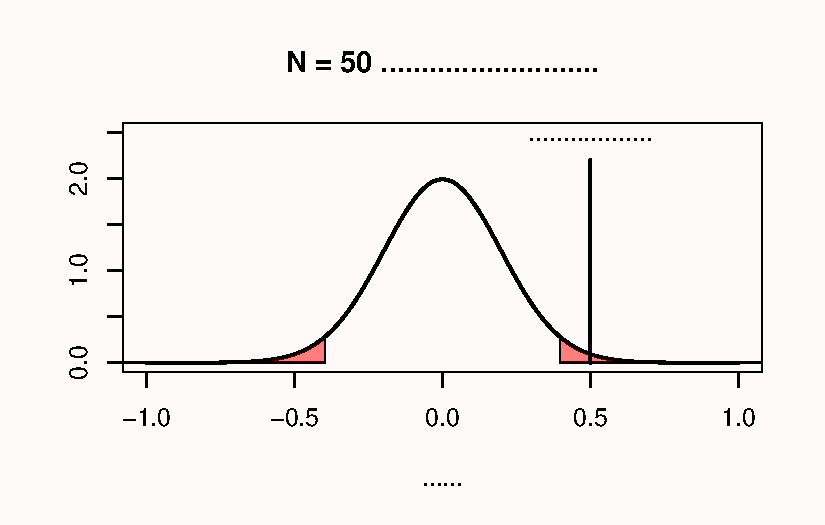
\includegraphics[width=1\textwidth,height=\textheight]{01-pvalue_files/figure-pdf/fig-fig137-1.pdf}

}

\caption{\label{fig-fig137}在\emph{d}= 0,对\emph{d} =
0.5进行每组50个观测值的独立样本\emph{t}检验中,所得Cohen's
\emph{d}效应量的分布}

\end{figure}

p值显著并不能让我们得出零假设(``随机数生成器照常运行'')为假的结论。的确,我们生成的50个样本的平均值是令人惊讶的极端值。但是较低的\emph{p}值只是告诉我们这个观测结果是出人意料的。当零假设为真时,我们只会在很低的概率下得到这个令人惊讶的观测结果------但它仍有可能发生。因此,显著的结果并不意味着备择假设就是对的------也有可能是出于Ⅰ型错误,就如同上面的例子,只有无所不知的琼斯知道是这种情况。

让我们重新审视这个错误陈述'\emph{p} \textless{}
.05,因此效应存在'。正确理解显著的\emph{p}值,要求我们承认显著结果是Ⅰ型错误的可能性。请记住,费希尔会得出的结论是''要么是发生了及其罕见的事件,要么是随机分布的原假设不正确''。对于内曼-皮尔逊统计的正确解释是:``我们可以当作零假设为假,从长远来看,我们错的时间不会超过5\%''。注意我们使用了'当作'这个词,这并不是在说任何特定的假设是真还是假,仅仅是指出,如果任何时候当\emph{p}
\textless{}
α,我们就当作零假设为假,那我们犯错误的频率将小于α百分比的时间。

这两种正式的陈述都有一点冗长。在科学文章中,我们经常读到简短点的陈述,比如:``我们可以拒绝零假设'',或者''我们可以接受备择假设''。这些陈述可能是假定读者会自己加上''长期来看,会有5\%的错误概率''这句话。但是,至少在第一次陈述时,可以加上''长期看有5\%的错误率''这个声明来提醒读者。

在上面的例子中,我们有一个非常强的主观先验概率,即R中的随机数生成器可以运行。其他可以纳入分析这种主观先验概率的统计方法有
\protect\hyperlink{bayes}{贝叶斯统计} 或者
\protect\hyperlink{ppv}{假阳报告概率}。在频率统计雪中,你需要多次重复你的研究。你会时不时地观测到Ⅰ类错误,但不太可能连续三次都观测到。或者,你也可以在单次研究中降低α水平,来降低犯Ⅰ类错误的概率。

\hypertarget{ux8befux89e3-3pux503cux663eux8457ux610fux5473ux7740ux53d1ux73b0ux4e86ux4e00ux4e2aux5b9eux9645ux91cdux8981ux7684ux6548ux5e94}{%
\subsection{\texorpdfstring{误解
3:\emph{p}值显著意味着发现了一个实际重要的效应。}{误解 3:p值显著意味着发现了一个实际重要的效应。}}\label{ux8befux89e3-3pux503cux663eux8457ux610fux5473ux7740ux53d1ux73b0ux4e86ux4e00ux4e2aux5b9eux9645ux91cdux8981ux7684ux6548ux5e94}}

在解释p值时,存在一个普遍的问题,即在日常语言中,``显著''意味着''重要'',因此''显著''的结果常被认为是一个''重要''的效应。然而,一个效应是否重要与它是否不等于零,或者说这个效应有多大是完全不同的两个问题。并不是所有的效应都用实际的影响。
这个效应越小,被人注意到的可能性就越小,但这个效应仍然可能会社会生产水平产生很大的影响。因此,正确的理解应该是,统计上的意义并不能回答一个效应在实践中是否重要,或者是否有''实际意义''的问题。要回答效应是否重要的问题,您需要进行成本效益分析。

这个实际意义的问题经常出现在样本量非常大的研究中。正如我们之前所看到的,随着样本量增加,零值周围的概率密度分布变得越来越窄,这被认为是\emph{p}值无限接近于0。

如果我们为一个非常大的样本量(例如,每组n=10000)绘制零模型,我们可以看到,即使是非常小的均值差(比0.04更极端的差异)也会被认为是''出人意料的''。这仍然意味着,如果在总体中真的没有差异,你观察到均值差大于0.04的将不到5\%的时间,在长期观测中,95\%的观测均值差将小于0.04。但是,要论证这种效应的实际意义就变得更加困难了。想象一下,一种特定的干预措施成功地改变了人们的消费行为,当实施这个干预措施时,人们每年可以节省12美分。很难说这种效应如何让任何一个个体感到开心。然而,如果把这笔资金加起来,它将产生超过200万美元,可用于治疗发展中国家的疾病,会产生很大的影响。如果我们的目标是让个人更快乐,干预的成本可能会被认为过高,但如果目标是为慈善机构筹集200万美元,它可能会被认为是值得的。

心理学中并不是所有的影响都是可以相加的(我们并不呢转移或者结合0.04的幸福感),因此往往很难论证主观感受中小效应的重要性(Anvari
et al.,
2021).。成本效益分析可能能显示很小的效应也很重要,但情况是否如此是不能从\emph{p}值中推断出来的。

请注意,这与对p值本身的解释并没有关系:如果零假设为真,p \textless{}
0.05仍然正确表明我们观测到的数据是出人意料的。然而,数据出人意料并不意味着我们就需要关心它。在这里造成困惑的主要是语言标签''显著''------``显著''应该理解为是''出乎意料的''效应,但不一定是''重要的''效应,这样想可能会减少困惑。

\hypertarget{sec-misconception4}{%
\subsection{误解
4:如果你得到了显著结果,你犯Ⅰ型错误(假阳性)的概率是5\%。}\label{sec-misconception4}}

此误解是对\emph{p}值是''偶然观察到显著结果的概率''这一错误说法的一种可能解释。试设想,我们收集了20个观测值,并且无所不知的琼斯告诉我们零假设为真(就像上面的例子里,我们在R中生成随机数一样)。这意味着我们正从下图的分布中进行抽样。

\begin{verbatim}
Warning in title(...): conversion failure on 'N = 20的零假设和备择假设' in
'mbcsToSbcs': dot substituted for <e7>
\end{verbatim}

\begin{verbatim}
Warning in title(...): conversion failure on 'N = 20的零假设和备择假设' in
'mbcsToSbcs': dot substituted for <9a>
\end{verbatim}

\begin{verbatim}
Warning in title(...): conversion failure on 'N = 20的零假设和备择假设' in
'mbcsToSbcs': dot substituted for <84>
\end{verbatim}

\begin{verbatim}
Warning in title(...): conversion failure on 'N = 20的零假设和备择假设' in
'mbcsToSbcs': dot substituted for <e9>
\end{verbatim}

\begin{verbatim}
Warning in title(...): conversion failure on 'N = 20的零假设和备择假设' in
'mbcsToSbcs': dot substituted for <9b>
\end{verbatim}

\begin{verbatim}
Warning in title(...): conversion failure on 'N = 20的零假设和备择假设' in
'mbcsToSbcs': dot substituted for <b6>
\end{verbatim}

\begin{verbatim}
Warning in title(...): conversion failure on 'N = 20的零假设和备择假设' in
'mbcsToSbcs': dot substituted for <e5>
\end{verbatim}

\begin{verbatim}
Warning in title(...): conversion failure on 'N = 20的零假设和备择假设' in
'mbcsToSbcs': dot substituted for <81>
\end{verbatim}

\begin{verbatim}
Warning in title(...): conversion failure on 'N = 20的零假设和备择假设' in
'mbcsToSbcs': dot substituted for <87>
\end{verbatim}

\begin{verbatim}
Warning in title(...): conversion failure on 'N = 20的零假设和备择假设' in
'mbcsToSbcs': dot substituted for <e8>
\end{verbatim}

\begin{verbatim}
Warning in title(...): conversion failure on 'N = 20的零假设和备择假设' in
'mbcsToSbcs': dot substituted for <ae>
\end{verbatim}

\begin{verbatim}
Warning in title(...): conversion failure on 'N = 20的零假设和备择假设' in
'mbcsToSbcs': dot substituted for <be>
\end{verbatim}

\begin{verbatim}
Warning in title(...): conversion failure on 'N = 20的零假设和备择假设' in
'mbcsToSbcs': dot substituted for <e5>
\end{verbatim}

\begin{verbatim}
Warning in title(...): conversion failure on 'N = 20的零假设和备择假设' in
'mbcsToSbcs': dot substituted for <92>
\end{verbatim}

\begin{verbatim}
Warning in title(...): conversion failure on 'N = 20的零假设和备择假设' in
'mbcsToSbcs': dot substituted for <8c>
\end{verbatim}

\begin{verbatim}
Warning in title(...): conversion failure on 'N = 20的零假设和备择假设' in
'mbcsToSbcs': dot substituted for <e5>
\end{verbatim}

\begin{verbatim}
Warning in title(...): conversion failure on 'N = 20的零假设和备择假设' in
'mbcsToSbcs': dot substituted for <a4>
\end{verbatim}

\begin{verbatim}
Warning in title(...): conversion failure on 'N = 20的零假设和备择假设' in
'mbcsToSbcs': dot substituted for <87>
\end{verbatim}

\begin{verbatim}
Warning in title(...): conversion failure on 'N = 20的零假设和备择假设' in
'mbcsToSbcs': dot substituted for <e6>
\end{verbatim}

\begin{verbatim}
Warning in title(...): conversion failure on 'N = 20的零假设和备择假设' in
'mbcsToSbcs': dot substituted for <8b>
\end{verbatim}

\begin{verbatim}
Warning in title(...): conversion failure on 'N = 20的零假设和备择假设' in
'mbcsToSbcs': dot substituted for <a9>
\end{verbatim}

\begin{verbatim}
Warning in title(...): conversion failure on 'N = 20的零假设和备择假设' in
'mbcsToSbcs': dot substituted for <e5>
\end{verbatim}

\begin{verbatim}
Warning in title(...): conversion failure on 'N = 20的零假设和备择假设' in
'mbcsToSbcs': dot substituted for <81>
\end{verbatim}

\begin{verbatim}
Warning in title(...): conversion failure on 'N = 20的零假设和备择假设' in
'mbcsToSbcs': dot substituted for <87>
\end{verbatim}

\begin{verbatim}
Warning in title(...): conversion failure on 'N = 20的零假设和备择假设' in
'mbcsToSbcs': dot substituted for <e8>
\end{verbatim}

\begin{verbatim}
Warning in title(...): conversion failure on 'N = 20的零假设和备择假设' in
'mbcsToSbcs': dot substituted for <ae>
\end{verbatim}

\begin{verbatim}
Warning in title(...): conversion failure on 'N = 20的零假设和备择假设' in
'mbcsToSbcs': dot substituted for <be>
\end{verbatim}

\begin{verbatim}
Warning in title(...): conversion failure on '差异' in 'mbcsToSbcs': dot
substituted for <e5>
\end{verbatim}

\begin{verbatim}
Warning in title(...): conversion failure on '差异' in 'mbcsToSbcs': dot
substituted for <b7>
\end{verbatim}

\begin{verbatim}
Warning in title(...): conversion failure on '差异' in 'mbcsToSbcs': dot
substituted for <ae>
\end{verbatim}

\begin{verbatim}
Warning in title(...): conversion failure on '差异' in 'mbcsToSbcs': dot
substituted for <e5>
\end{verbatim}

\begin{verbatim}
Warning in title(...): conversion failure on '差异' in 'mbcsToSbcs': dot
substituted for <bc>
\end{verbatim}

\begin{verbatim}
Warning in title(...): conversion failure on '差异' in 'mbcsToSbcs': dot
substituted for <82>
\end{verbatim}

\begin{verbatim}
Warning in text.default(0.5, 2.4, paste("所得均值差异"), cex = 1): conversion
failure on '所得均值差异' in 'mbcsToSbcs': dot substituted for <e6>
\end{verbatim}

\begin{verbatim}
Warning in text.default(0.5, 2.4, paste("所得均值差异"), cex = 1): conversion
failure on '所得均值差异' in 'mbcsToSbcs': dot substituted for <89>
\end{verbatim}

\begin{verbatim}
Warning in text.default(0.5, 2.4, paste("所得均值差异"), cex = 1): conversion
failure on '所得均值差异' in 'mbcsToSbcs': dot substituted for <80>
\end{verbatim}

\begin{verbatim}
Warning in text.default(0.5, 2.4, paste("所得均值差异"), cex = 1): conversion
failure on '所得均值差异' in 'mbcsToSbcs': dot substituted for <e5>
\end{verbatim}

\begin{verbatim}
Warning in text.default(0.5, 2.4, paste("所得均值差异"), cex = 1): conversion
failure on '所得均值差异' in 'mbcsToSbcs': dot substituted for <be>
\end{verbatim}

\begin{verbatim}
Warning in text.default(0.5, 2.4, paste("所得均值差异"), cex = 1): conversion
failure on '所得均值差异' in 'mbcsToSbcs': dot substituted for <97>
\end{verbatim}

\begin{verbatim}
Warning in text.default(0.5, 2.4, paste("所得均值差异"), cex = 1): conversion
failure on '所得均值差异' in 'mbcsToSbcs': dot substituted for <e5>
\end{verbatim}

\begin{verbatim}
Warning in text.default(0.5, 2.4, paste("所得均值差异"), cex = 1): conversion
failure on '所得均值差异' in 'mbcsToSbcs': dot substituted for <9d>
\end{verbatim}

\begin{verbatim}
Warning in text.default(0.5, 2.4, paste("所得均值差异"), cex = 1): conversion
failure on '所得均值差异' in 'mbcsToSbcs': dot substituted for <87>
\end{verbatim}

\begin{verbatim}
Warning in text.default(0.5, 2.4, paste("所得均值差异"), cex = 1): conversion
failure on '所得均值差异' in 'mbcsToSbcs': dot substituted for <e5>
\end{verbatim}

\begin{verbatim}
Warning in text.default(0.5, 2.4, paste("所得均值差异"), cex = 1): conversion
failure on '所得均值差异' in 'mbcsToSbcs': dot substituted for <80>
\end{verbatim}

\begin{verbatim}
Warning in text.default(0.5, 2.4, paste("所得均值差异"), cex = 1): conversion
failure on '所得均值差异' in 'mbcsToSbcs': dot substituted for <bc>
\end{verbatim}

\begin{verbatim}
Warning in text.default(0.5, 2.4, paste("所得均值差异"), cex = 1): conversion
failure on '所得均值差异' in 'mbcsToSbcs': dot substituted for <e5>
\end{verbatim}

\begin{verbatim}
Warning in text.default(0.5, 2.4, paste("所得均值差异"), cex = 1): conversion
failure on '所得均值差异' in 'mbcsToSbcs': dot substituted for <b7>
\end{verbatim}

\begin{verbatim}
Warning in text.default(0.5, 2.4, paste("所得均值差异"), cex = 1): conversion
failure on '所得均值差异' in 'mbcsToSbcs': dot substituted for <ae>
\end{verbatim}

\begin{verbatim}
Warning in text.default(0.5, 2.4, paste("所得均值差异"), cex = 1): conversion
failure on '所得均值差异' in 'mbcsToSbcs': dot substituted for <e5>
\end{verbatim}

\begin{verbatim}
Warning in text.default(0.5, 2.4, paste("所得均值差异"), cex = 1): conversion
failure on '所得均值差异' in 'mbcsToSbcs': dot substituted for <bc>
\end{verbatim}

\begin{verbatim}
Warning in text.default(0.5, 2.4, paste("所得均值差异"), cex = 1): conversion
failure on '所得均值差异' in 'mbcsToSbcs': dot substituted for <82>
\end{verbatim}

\begin{verbatim}
Warning in text.default(0.5, 2.4, paste("所得均值差异"), cex = 1): font metrics
unknown for Unicode character U+6240
\end{verbatim}

\begin{verbatim}
Warning in text.default(0.5, 2.4, paste("所得均值差异"), cex = 1): font metrics
unknown for Unicode character U+5f97
\end{verbatim}

\begin{verbatim}
Warning in text.default(0.5, 2.4, paste("所得均值差异"), cex = 1): font metrics
unknown for Unicode character U+5747
\end{verbatim}

\begin{verbatim}
Warning in text.default(0.5, 2.4, paste("所得均值差异"), cex = 1): font metrics
unknown for Unicode character U+503c
\end{verbatim}

\begin{verbatim}
Warning in text.default(0.5, 2.4, paste("所得均值差异"), cex = 1): font metrics
unknown for Unicode character U+5dee
\end{verbatim}

\begin{verbatim}
Warning in text.default(0.5, 2.4, paste("所得均值差异"), cex = 1): font metrics
unknown for Unicode character U+5f02
\end{verbatim}

\begin{figure}

{\centering 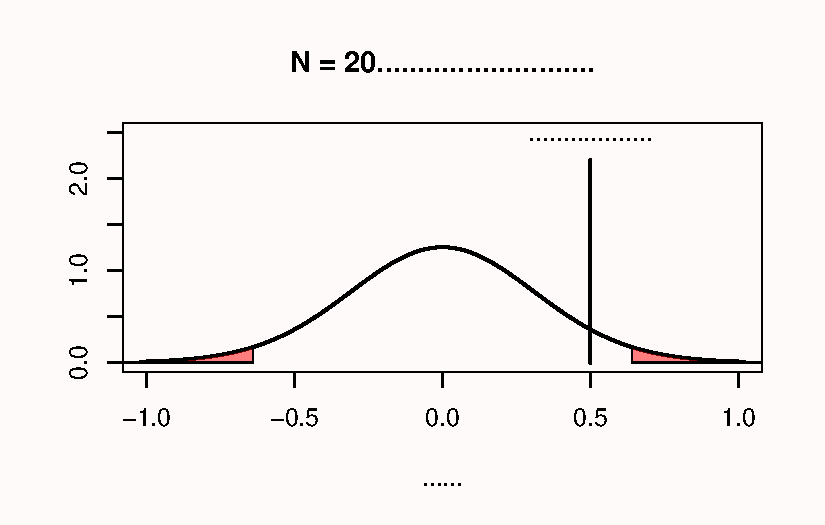
\includegraphics[width=1\textwidth,height=\textheight]{01-pvalue_files/figure-pdf/fig-fig138-1.pdf}

}

\caption{\label{fig-fig138}\emph{d}=0,在每组20个观测值的独立样本\emph{t}检验中,Cohen's
\emph{d}效应量的分布。}

\end{figure}

如果这是真实情况,那意味着100\%的时间里发现的显著结果,都是假阳性(或者犯了Ⅰ型错误)。因此,100\%的显著结果都是Ⅰ型错误导致的。

区分数据收集和结果分析之前和之后的概率是非常重要的。犯Ⅰ型错误的概率是指,在未来可能完成的所有零假设为真的研究中,低于5\%的观测到的均值差会落到分布的红色尾部区域。但是当观测的结果落到了尾部区域,\emph{p}\textless α,我们又知道零假设为真时,那么这些显著结果就是Ⅰ型错误导致的。如果阅读得足够仔细,你就会发现这个误解实际是设问方式不同导致的。``如果我发现\emph{p}\textless.05,零假设为真的概率是多少?''和''如果零假设为真,观察到显著结果的概率是多少?``是两个完全不同的问题。\emph{p}值只回答后一个问题。第一个问题在数据收集前没有主观判断零假设为真时是无法回答的。

\hypertarget{ux8befux89e3-51ux51cfux53bbpux503cux662fux91cdux590dux5b9eux9a8cux80fdux5f97ux5230ux76f8ux540cux6548ux5e94ux7684ux6982ux7387}{%
\subsection{\texorpdfstring{误解
5:1减去\emph{p}值是重复实验能得到相同效应的概率。}{误解 5:1减去p值是重复实验能得到相同效应的概率。}}\label{ux8befux89e3-51ux51cfux53bbpux503cux662fux91cdux590dux5b9eux9a8cux80fdux5f97ux5230ux76f8ux540cux6548ux5e94ux7684ux6982ux7387}}

我们不可能计算出一种效应重复出现的概率 (Miller,
2009),因为存在太多未知的因素影响效应重复的概率,其中最主要的因素就是真均值差。如果我们是无所不知的琼斯,知道真均值差的值(例如,两组之间的差异为0.5分),我们就能知道这个检验的统计力。统计检验力是指当备择假设为真时(即,效应存在),我们能发现显著结果的概率。例如,阅读应用程序中左侧栏里的文本,我们可以发现每组的样本量为50,α水平为0.05,真均值差为0.5,发现显著结果(或称统计检验力)的概率为69.69\%
。
如果我们在这种情况下观察到显著的效应(例如,\emph{p}=0.03),并不意味着我们有97\%的可能重复该次研究(样本量相同)也会得到显著的结果。重复研究得到显著结果的概率取决于统计检验力,而非之前研究的\emph{p}值。

我们可以从最后一个误解中得到的事实是,显著结果复现的概率取决于真实的效应是否存在。换句话说,像上面的例子一样,如果存在一个真实的效应,统计检验力的水平就代表着能够重复观察到显著结果的概率(例如,统计检验力为80\%意味着我们有80\%的时间能够观察到显著的结果)。另一方面,如果零假设为真(例如,效应为0),那么显著的结果仅仅会在接近我们选择的α水平的概率上被观察到(例如,如果α为0.05,就有5\%的可能犯Ⅰ型错误)。因此,如果原始研究中正确地观测到了一个效应,在重复实验中观察到显著结果的概率取决于统计检验力;如果原始研究中正确地观测到了零效应,在重复实验中观察到显著结果的概率则取决于α水平。
在实践中,还存在很多其他因素决定效应是否能重复。判断效应能否重复的唯一方法就是去复现实验。如果你想要知道判断文献里的结果能否复现有多难,你可以\href{https://80000hours.org/psychology-replication-quiz/}{在80小时内重复此实验}。

\hypertarget{ux81eaux6211ux6d4bux8bd5}{%
\section{自我测试}\label{ux81eaux6211ux6d4bux8bd5}}

\#\#\#你能想到的有关p值的问题

将下面的代码复制到 R
并运行代码。您可以单击代码部分右上角的``剪贴板''图标,将所有代码复制到剪贴板,这样您就可以轻松地将其粘贴到
R 中。

\begin{Shaded}
\begin{Highlighting}[]
\NormalTok{nsims }\OtherTok{\textless{}{-}} \DecValTok{100000} \CommentTok{\# number of simulations}
\CommentTok{\# 模拟的次数}

\NormalTok{m }\OtherTok{\textless{}{-}} \DecValTok{106} \CommentTok{\# mean sample}
\CommentTok{\# 样本均值}
\NormalTok{n }\OtherTok{\textless{}{-}} \DecValTok{26} \CommentTok{\# set sample size}
\CommentTok{\# 设置样本量大小}
\NormalTok{sd }\OtherTok{\textless{}{-}} \DecValTok{15} \CommentTok{\# SD of the simulated data}
\CommentTok{\#模拟数据的标准差}

\NormalTok{p }\OtherTok{\textless{}{-}} \FunctionTok{numeric}\NormalTok{(nsims) }\CommentTok{\# set up empty vector}
\CommentTok{\# 设置一个空向量}
\NormalTok{bars }\OtherTok{\textless{}{-}} \DecValTok{20}

\ControlFlowTok{for}\NormalTok{ (i }\ControlFlowTok{in} \DecValTok{1}\SpecialCharTok{:}\NormalTok{nsims) \{ }\CommentTok{\# for each simulated experiment}
  \CommentTok{\# 对于每次模拟实验的循环}
\NormalTok{  x }\OtherTok{\textless{}{-}} \FunctionTok{rnorm}\NormalTok{(}\AttributeTok{n =}\NormalTok{ n, }\AttributeTok{mean =}\NormalTok{ m, }\AttributeTok{sd =}\NormalTok{ sd)}
\NormalTok{  z }\OtherTok{\textless{}{-}} \FunctionTok{t.test}\NormalTok{(x, }\AttributeTok{mu =} \DecValTok{100}\NormalTok{) }\CommentTok{\# perform the t{-}test  \# 进行T检验}
\NormalTok{  p[i] }\OtherTok{\textless{}{-}}\NormalTok{ z}\SpecialCharTok{$}\NormalTok{p.value }\CommentTok{\# get the p{-}value  \#得到p值}
\NormalTok{\}}
\NormalTok{power }\OtherTok{\textless{}{-}} \FunctionTok{round}\NormalTok{((}\FunctionTok{sum}\NormalTok{(p }\SpecialCharTok{\textless{}} \FloatTok{0.05}\NormalTok{) }\SpecialCharTok{/}\NormalTok{ nsims), }\DecValTok{2}\NormalTok{) }\CommentTok{\# power \# 统计功效}

\CommentTok{\# Plot figure \# 画图}
\FunctionTok{hist}\NormalTok{(p,}
  \AttributeTok{breaks =}\NormalTok{ bars, }\AttributeTok{xlab =} \StringTok{"P{-}values"}\NormalTok{, }\AttributeTok{ylab =} \StringTok{"number of p{-}values}\SpecialCharTok{\textbackslash{}n}\StringTok{"}\NormalTok{, }
  \AttributeTok{axes =} \ConstantTok{FALSE}\NormalTok{, }\AttributeTok{main =} \FunctionTok{paste}\NormalTok{(}\StringTok{"P{-}value Distribution with"}\NormalTok{, }
                             \FunctionTok{round}\NormalTok{(power }\SpecialCharTok{*} \DecValTok{100}\NormalTok{, }\AttributeTok{digits =} \DecValTok{1}\NormalTok{), }\StringTok{"\% Power"}\NormalTok{),}
  \AttributeTok{col =} \StringTok{"grey"}\NormalTok{, }\AttributeTok{xlim =} \FunctionTok{c}\NormalTok{(}\DecValTok{0}\NormalTok{, }\DecValTok{1}\NormalTok{), }\AttributeTok{ylim =} \FunctionTok{c}\NormalTok{(}\DecValTok{0}\NormalTok{, nsims))}
\FunctionTok{axis}\NormalTok{(}\AttributeTok{side =} \DecValTok{1}\NormalTok{, }\AttributeTok{at =} \FunctionTok{seq}\NormalTok{(}\DecValTok{0}\NormalTok{, }\DecValTok{1}\NormalTok{, }\FloatTok{0.1}\NormalTok{), }\AttributeTok{labels =} \FunctionTok{seq}\NormalTok{(}\DecValTok{0}\NormalTok{, }\DecValTok{1}\NormalTok{, }\FloatTok{0.1}\NormalTok{))}
\FunctionTok{axis}\NormalTok{(}\AttributeTok{side =} \DecValTok{2}\NormalTok{, }\AttributeTok{at =} \FunctionTok{seq}\NormalTok{(}\DecValTok{0}\NormalTok{, nsims, nsims }\SpecialCharTok{/} \DecValTok{4}\NormalTok{), }
     \AttributeTok{labels =} \FunctionTok{seq}\NormalTok{(}\DecValTok{0}\NormalTok{, nsims, nsims }\SpecialCharTok{/} \DecValTok{4}\NormalTok{), }\AttributeTok{las =} \DecValTok{2}\NormalTok{)}
\FunctionTok{abline}\NormalTok{(}\AttributeTok{h =}\NormalTok{ nsims }\SpecialCharTok{/}\NormalTok{ bars, }\AttributeTok{col =} \StringTok{"red"}\NormalTok{, }\AttributeTok{lty =} \DecValTok{3}\NormalTok{)}
\end{Highlighting}
\end{Shaded}

\begin{figure}[H]

{\centering 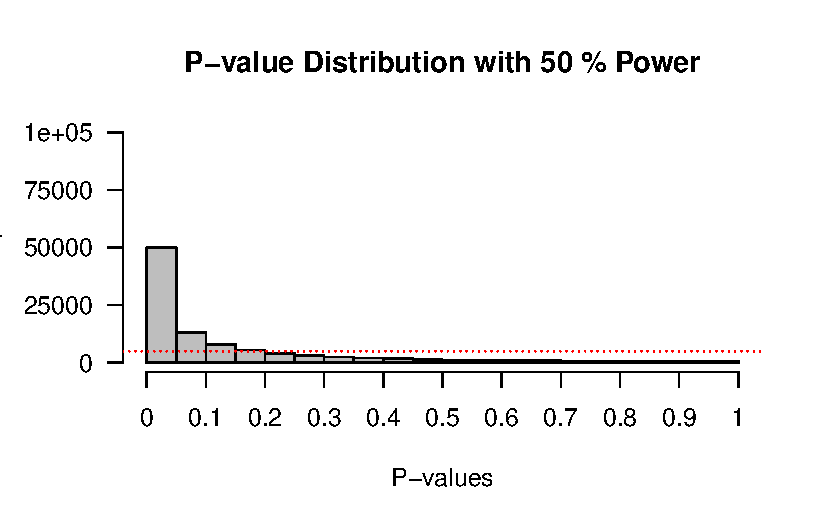
\includegraphics[width=1\textwidth,height=\textheight]{01-pvalue_files/figure-pdf/q1-1.pdf}

}

\end{figure}

我们可以从条形图的x轴上看到从 0 到 1 的 p 值,在 y 轴上,我们能看到这些
p 值的频率。其中水平红色虚线表示 alpha 为 5\%(位于频率 100.000*0.05 =
5000)------但您现在可以忽略这条线。在标题中,给出了在模拟研究中达到的统计功效(假设
alpha 为 0.05):研究具有 50\% 的功效(每次模拟都有细微的差异)。

\textbf{问题1}:由于统计功效是观察到一个具有统计显着性结果的概率,如果效应为真,我们从该图上哪里以看到统计功效本身?

\begin{enumerate}
\def\labelenumi{\Alph{enumi})}
\tightlist
\item
  我们可以计算出大于 0.5 的 p 值的数量,并将它们除以模拟次数。
\item
  我们可以计算第一个条形中的 p 值数量(其中包含从 0.00 到 0.05
  的所有``显着''p 值),并将该条形中的 p 值除以模拟总数。
\item
  我们可以计算高于 0.5 的 p 值减去低于 0.5 的 p
  值之间的差值,并将该数字除以模拟总数。
\item
  我们可以计算高于 0.5 的 p 值减去低于 0.05 的 p
  值之间的差值,并将该数字除以模拟次数。
\end{enumerate}

\textbf{问题2}:将代码中第 4 行的样本大小从 n = 26 更改为 n =
51。通过选择所有行并按 CTRL+Enter 来运行模拟。现在我们已将样本量从 26
人增加到
51人,模拟的功效如何?请记住,模拟有时会产生略有不同的答案,因此请选择最接近模拟结果的答案选项。

\begin{enumerate}
\def\labelenumi{\Alph{enumi})}
\tightlist
\item
  55\%
\item
  60\%
\item
  80\%
\item
  95\%
\end{enumerate}

\textbf{问题3}:如果你观察p值的分布,你会发现什么?

\begin{enumerate}
\def\labelenumi{\Alph{enumi})}
\tightlist
\item
  p值分布与 50\% 功效完全相同
\item
  p值分布比 50\% 功效陡峭得多
\item
  p值分布比 50\% 功效平坦得多
\item
  p值分布比 50\% 功效更符合正态分布
\end{enumerate}

请随意增加和减少样本量,看看运行后会发生什么。完成这些探索后,请确保第4行代码中的样本量仍然为
n = 51。

\textbf{问题4}:当我们的模拟样本与平均 IQ
分数之间没有真正差异时会发生什么?在这种情况下,我们没有观察到任何效应,因此您可能会说功效为``0''。事实上,当没有真正的效应不存在时,统计功效的确无法被定义。但是,我们可以因此将其称为``零功效''。将样本中的均值更改为
100(将 m = 106 设置为 m = 100), 现在样本中的均值与我们在单样本 t
检验中测试的总体值之间没有差异。请再次运行脚本,您发现了什么?

\begin{enumerate}
\def\labelenumi{\Alph{enumi})}
\tightlist
\item
  p 值分布与 50\% 功效完全相同
\item
  p 值分布比 50\% 功效陡峭得多
\item
  p
  值分布基本上是完全平坦的(忽略了由于模拟中的随机噪声引起的一些微小变化)
\item
  p 值分布呈正态(即钟形)分布
\end{enumerate}

下面的问题建立在上面的数据模拟之上,其中各组之间没有真正的区别。

\textbf{问题5}:查看为Q4生成的图中最左边的条柱,并查看该条中p值的频率。这个条柱的正式名称应该是什么?

\begin{enumerate}
\def\labelenumi{\Alph{enumi})}
\tightlist
\item
  功效(或真阳性)
\item
  真阴性
\item
  I类错误(或假阳性)
\item
  II类错误(或假阴性)
\end{enumerate}

让我们只看一下低于 0.05 的 p 值,请耐心进行接下来的几个步骤。在第 8
行的语句 bars = 20 中找到决定有多少条柱的变量。将其更改为 bars =
100。我们现在将获得 0 到 0.01 之间的 p 值的 1 个柱,p值在 0.01 和 0.02
之间的1个柱,总共 100 个柱。红色虚线现在将指示原假设为真时 p
值的频率,其中每个条柱包含 p 值总数的 1\%。我们只想查看低于 0.05 的 p
值,我们将在 0.05 处截断该图。将 xlim = c(0, 1) 更改为 xlim = c(0,
0.05)。我们不会看到 0 到 1 之间的所有 p 值,而只会看到 0 到 0.05 之间的
p 值。重新运行模拟(仍然是 m \textless-
100)。我们将看到相同的均匀分布,但现在每个条柱都包含 1\% 的 p 值,因此
p 值分布非常平坦,几乎看不到(稍后我们将在 y
轴上放大此分布)。假设零假设为真,红线现在清楚地给出了每个条柱的频率。

将第9行模拟中的平均值更改为 m \textless- 107(记住 n 仍然是
51)。重新运行模拟。很明显,我们拥有非常大的功效。大多数p值位于最左侧的条柱中,其中包含
0.00 和 0.01 之间的所有 p 值。

\textbf{问题6}:上次模拟的图告诉我们有大约 90.5\%
的功效(注意:由于随机变化,您模拟中的数字可能会略有不同),这就是我们使用
5\% 的alpha时的功效。但我们也可以使用 1\% 的 alpha。看看图表,当我们使用
1\% 的 alpha
时,我们在模拟研究中的统计功效是多少?从您的模拟中选择最接近答案的答案。请注意,您还可以通过将第
15 行中的 p \textless{} 0.05 更改为 p \textless{} 0.01
来计算alpha为0.01的统计功效,只需确保在继续下一步探索之前将其设置回
0.05。

\begin{enumerate}
\def\labelenumi{\Alph{enumi})}
\tightlist
\item
  \textasciitilde90\%
\item
  \textasciitilde75\%
\item
  \textasciitilde50\%
\item
  \textasciitilde5\%
\end{enumerate}

为了能够查看 0.03 和 0.04 附近的 p 值,我们还将放大 y
轴。在绘制绘图的代码部分,将 ylim = c(0, nSims) 更改为 ylim = c(0,
10000)。重新运行脚本。

将样本中的平均值更改为 108,m \textless- 108),并将样本大小保留为
51。运行模拟。与上图相比,看看分布发生了怎样的变化?

查看从左边数第五个条柱。此条柱现在包含 0.04 到 0.05 之间的所有 p
值。你可能会发现一些奇怪的现象。请记住,假设零假设为真,红色虚线表示每个条中的频率。查看
p 值介于 0.04 和 0.05 之间的条形如何低于红线。我们有 96\%
功效的模拟研究。当功效非常高时,p 值介于 0.04 和 0.05
之间的情况非常罕见------它们出现的概率不到 1\%(大多数 p 值小于
0.01)。当原假设为真时,0.04 和 0.05 之间的 p 值恰好出现 1\%
的几率(因为 p
值是均匀分布的)。现在问问自己:当您的统计功效非常高并且观察到 p 值介于
0.04 和 0.05
之间时,零假设更可能为真,还是备择假设更可能为真?鉴于当原假设为真时您更有可能观察到
0.04 和 0.05 之间的 p 值,而不是当备择假设为真时,您应该将 alpha 为 0.05
的 p 值解释为更有可能当原假设为真时为真,而不是备择假设为真。

在我们的模拟中,我们知道是否存在真实的效应,但在现实世界中,我们往往不知道。当您具有非常高的统计功效时,使用
0.05 的 alpha 水平,并找到 p = .045 的 p
值,数据令人吃惊。假设原假设为真,但更令人惊讶的是,假设备择假设是真的。这表明显着的
p 值并不总是备择假设的证据。

\textbf{问题7}:当您知道您对您关心的最小效应量具有非常高(例如
98\%)的功效,并且您观察到 p 值为 0.045 时,正确的结论是什么?

\begin{enumerate}
\def\labelenumi{\Alph{enumi})}
\tightlist
\item
  效应显着,为备择假设提供了强有力的支持。
\item
  效应显着,但毫无疑问属于第一类错误。
\item
  对于高统计功效,应该使用小于 0.05 的 alpha
  水平,因此,该效应不能被认为是显着的。
\item
  效应显着,但数据在原假设下比在备择假设下更有可能。
\end{enumerate}

\textbf{问题8}:通过改变样本量 (n) 和平均值
(m),从而改变模拟研究中的统计功效。查看包含介于 0.04 和 0.05 之间的 p
值的条形的模拟结果。红线表示如果零假设为真(并且始终为
1\%),将在此条柱中找到多少 p 值。在最好的情况下,0.04 和 0.05 之间的 p
值来自表示真实效果的 p 值分布的可能性比来自没有效果的 p
值分布的可能性大多少?您可以通过查看 0.04 和 0.05 之间的 p
值条可以变得多高来回答这个问题。如果模拟中的条形图最多是红线处的五倍高(因此条形图显示
5\% 的 p 值最终介于 0.04 和 0.05 之间,而红线保持在 1\%),那么最好的
p-值在 0.04 和 0.05 之间时,有真实效应的可能性是没有真实效应时的五倍。

\begin{enumerate}
\def\labelenumi{\Alph{enumi})}
\tightlist
\item
  0.04 和 0.05 之间的 p 值在备择假设和零假设下的可能性相同。
\item
  在替代假设下,p 值介于 0.04 和 0.05 之间的可能性大约是零假设下的 4
  倍。
\item
  在替代假设下,p 值介于 0.04 和 0.05 之间的可能性是零假设下的 10
  倍左右。
\item
  在备择假设下,p 值介于 0.04 和 0.05 之间的可能性最多是零假设下的 30
  倍。
\end{enumerate}

出于这个原因,统计学家会发出警告:略低于 0.05 的 p 值(例如,0.04 和
0.05 之间)是对备择假设的最弱支持。如果您发现 p
值在此范围内,请考虑重复该研究,或者如果这不可能,至少要谨慎地解释结果。当然,您可以在
Neyman-Pearson 方法中提出最多 5\% Type 1
错误率的声明。因此,林德利悖论很好地说明了统计推断的不同哲学方法之间的差异。

\hypertarget{ux9488ux5bf9pux503cux6982ux5ff5ux7684ux8befux89e3}{%
\subsection{针对p值概念的误解}\label{ux9488ux5bf9pux503cux6982ux5ff5ux7684ux8befux89e3}}

\textbf{问题1}:当独立t检验中每组的样本量为50个观察值时(见图@fig-fig131),下面哪种说法是正确的?

\begin{enumerate}
\def\labelenumi{\Alph{enumi})}
\tightlist
\item
  两组之间观察到平均差异总是0。
\item
  两组之间的平均差异一般不可能为0。
\item
  假设零假设为真,能观察到+0.5或-0.5的平均差异几乎不太可能
\item
  假设零假设为真,能观察到+0.1或-0.1的平均差异几乎不太可能
\end{enumerate}

\textbf{问题2}:图 Figure~\ref{fig-fig131} 和图 Figure~\ref{fig-fig132}
中的零模型在什么方面上是相似的,在什么方面又是不同的?

\begin{enumerate}
\def\labelenumi{\Alph{enumi})}
\tightlist
\item
  在这两种情况下,分布都以零为中心,临界t值在1.96和2之间(对于双侧检验来说,取决于样本量)。但是,样本量越大,被认为
  ``令人惊讶''的平均差异就越接近于0。
\item
  在这两种情况下,t值为0是最有可能的结果,但临界t值对于n=50来说大约是0.4,对于n=5000来说大约是0.05。
\item
  在这两种情况下,平均值在0附近的变化方式完全相同,但是n=5000时的犯第一类错误的概率比n=50时小得多。
\item
  因为n=50的标准误差比n=5000的标准误差大得多,所以n=50的零假设更可能是真的。
\end{enumerate}

\textbf{问题3}:您可以在这个在线app中玩玩替代模型和空模型:http://shiny.ieis.tue.nl/d\_p\_power/。
该应用程序允许你指定独立t检验中每组的样本量(从2到无穷大),平均差异(从0到2),以及α水平。在该图中,红色区域显示了第一类错误。蓝色区域直观地显示了第二类错误率。该app还会告诉你临界值:
有一条垂直线(在n=50的情况下,这条线落在0.4的平均差上)和一个标签,说:``大于0.4的效应将具有统计学意义''。请注意,对于小于-0.4的效应也是如此,尽管那里没有第二个标签,但该app显示了双侧独立t检验的情况。

您可以看到,在表示临界均值差的垂直线左侧,有一个蓝色区域是备择假设模型的一部分。这是
犯II类错误的几率(或表示1 减去该研究的统计功效)。如果一项研究具有 80\%
的功效,那么我们将观察到的 80\%
的平均误差应该落在该线指示的临界值的右侧。如果备择假设的模型为真,但我们观察到的效应小于临界值,即使存在真实效应,那么我们观察到的p值也将大于
0.05,您可以在 app
中查看,效应越大,整个备择假设所代表的模型分布越靠右,因此统计功效越高。您还可以看到,样本量越大,分布越窄,低于临界值的分布将越少(只要真正的总体均值大于临界值)。最后,alpha
水平越大,临界均值差向左移动得越远,低于临界值的备择假设所代表的分布区域就越小。

该app还绘制了3张图表,说明作为不同α水平、样本量或真实平均差的函数的统计功效曲线。通过改变数值,在app中进行探索。感受一下每个变量是如何影响零模型和备择模型的,以及如何影响具有统计学意义的平均差、I类和II类错误率的。

打开app,并确保它为默认设置,即保持样本量为50,α水平为0.05。看一下零模型的分布。然后将样本大小设为2,再将样本大小设为5000并观察分布。在该app中,你无法绘制''组''样本量大小为1的数据。但在n
= 2的情况下,你将得到真实效应为0时单个观察值(n =
1)的期望值范围。鉴于你在改变不同参数时对app的体验,下面哪句话是真的?

\begin{enumerate}
\def\labelenumi{\Alph{enumi})}
\tightlist
\item
  当零假设为真且标准差为1时,如果你从每组中随机抽取1个观察值并计算差异得分,那么在你将抽取的95\%的观察对中,差异将落在-0.4和0.4之间。
\item
  当零假设为真,标准差为1时,每组样本量n=50,95\%的研究数据在长期内将被观察到均值差落在-0.4和0.4之间。
\item
  在任意每组样本量为n=50的研究中,即使标准差未知,并且也不知道零假设是否为真,你应该很少观察到比-0.4或0.4更极端的均值差异。
\item
  随着样本量的增加,对于零模型来说,均值的期望分布会变窄,但对于备择模型来说则不会。
\end{enumerate}

\textbf{问题4} 使用默认设置再次打开应用程序。将 alpha 水平设置为
0.01(同时将平均差保持在 0.5,样本大小保持在50)。与 alpha = 0.05
时的临界值相比,以下哪个说法是正确的?

\begin{enumerate}
\def\labelenumi{\Alph{enumi})}
\tightlist
\item
  与0.05的α值相比,当使用0.01的α值时,只有不太极端的数值才会被认为是令人难以置信的,而且现在只有大于0.53(或小于-0.53)的差异才会具备统计学意义。
\item
  与0.05的α值相比,当使用0.01的α值时,只有较少的极端值被认为是令人难以置信的,而且现在只有大于0.33(或小于-0.33)的差异才会具备统计学意义。
\item
  与0.05的α值相比,当使用0.01的α值时,只有更多的极端值被认为是令人难以置信的,而且只有大于0.53(或小于-0.53)的差异才具备统计学意义。
\item
  与0.05的α值相比,当使用0.01的α值时,只有更多的极端值被认为是令人难以置信的,而且现在只有大于0.33(或小于-0.33)的差异才会具备统计学意义。
\end{enumerate}

\textbf{问题5} 当您观察到统计上不显著的 p 值 (p \textgreater{} α)
时,为什么不能得出零假设一定为真的结论?

\begin{enumerate}
\def\labelenumi{\Alph{enumi})}
\tightlist
\item
  在计算p值时,你总是需要考虑到先验概率。
\item
  你需要意识到你观察到I类错误的概率。
\item
  零假设永远不会是真的。
\item
  你需要意识到你观察到II类错误的概率。
\end{enumerate}

\textbf{问题6:} 当你观察到一个具有统计学意义的p值(p \textless{}
α)时,为什么不能得出备择假设一定为真的结论?

\begin{enumerate}
\def\labelenumi{\Alph{enumi})}
\tightlist
\item
  在计算p值时,你总是需要考虑到先验概率。
\item
  你需要意识到你观察到的I类错误的概率。
\item
  备择假设从不为真。
\item
  你需要意识到你观察到II类错误的概率。
\end{enumerate}

\textbf{问题7:}
在解释p值时,一个常见的问题是,``显著''在正常语言中意味着
``重要'',因此,``显著''效应被解释为
``重要''效应。然而,一个效应是否重要的问题与它是否不等于零,甚至效应有多大的问题是完全独立的。一方面来说,不是所有的效应在实际生活中都能产生影响。另外一方面来说,效应越小,越不可能被人注意到,但这种效应仍然可能在社会层面上产生很大的影响。因此,一般来说,统计学意义并不能回答一个效应在实践中是否重要,或是否
``实际重要''的问题。要回答一个效应是否重要的问题,你需要做成本效益分析。

转到app:http://shiny.ieis.tue.nl/d\_p\_power/。设置样本量为50000,平均差异为0.5,α水平为0.05,并观察以下哪种效应会与0存在统计学差异?

\begin{enumerate}
\def\labelenumi{\Alph{enumi})}
\tightlist
\item
  比-0.01和0.01更极端的效应
\item
  比-0.04和0.04更极端的效应
\item
  比-0.05和0.05更极端的效应
\item
  比-0.12和0.12更极端的效应
\end{enumerate}

如果我们为一个非常大的样本量(例如,每组n=10000)绘制零模型,我们会发现,即使是非常小的平均差异(比0.04的平均差异更极端的差异)也会被认为是''令人惊喜的''。这仍然意味着,如果在整个人群中真的没有差异,你将有5\%的几率观察到大于0.04的平均差异,而剩下95\%的几率则观察到小于0.04的平均差异。但要论证这种效应的实际意义就变得更加困难。想象一下,一项具体的干预措施在改变人们的消费行为方面是成功的,当实施某种干预措施时,人们每年可以节省12美分。很难论证这种效应如何使人更加幸福。然而,如果这些钱加在一起,将产生200多万,这些钱可以用于治疗发展中国家的疾病,在那里会产生真正的影响。而如果干预的目标是使个人更快乐,干预的成本可能被认为太高,但如果目标是为慈善事业筹集200万,可能会被认为是值得的。

在心理学中,并不是所有的效应都是相加的(我们不能将幸福感增加0.04个尺度点的效应合并或转换),所以要论证主观感受中的小效应的重要性往往比较困难。成本效益分析可能显示小效应很重要,但是否真的如此,我们不能从p值中推断出来。相反,您需要报告并解释效应量。

\textbf{问题8:} 我们使用R语言中的随机数生成器,输入rnorm(n = 50, mean =
0, sd =
1)生成50个观察值,这些观察值的平均值是0.5,在对效应为0的单样本t检验中得到的p值是0.03,小于α水平(我们设定为0.05)。我们观察到显著差异(p\textless α)只是偶然的概率有多少?

\begin{enumerate}
\def\labelenumi{\Alph{enumi})}
\tightlist
\item
  3\%
\item
  5\%
\item
  95\%
\item
  100\%
\end{enumerate}

\textbf{问题9:} 以下哪一个说法是正确的?

\begin{enumerate}
\def\labelenumi{\Alph{enumi})}
\tightlist
\item
  重复研究产生显著结果的概率为1-p。
\item
  重复研究产生显著结果的概率是1-p乘以零假设为真的概率。
\item
  重复研究产生显著结果的概率等于重复研究的统计功效(如果存在真实效应的话)或α水平(如果不存在真实效应)。
\item
  重复研究产生显著结果的概率等于重复研究的统计功效加上α水平。
\end{enumerate}

这个问题在概念上与Tversky和(1971) 在
``相信小数法则''一文中提出的问题非常相似:

\begin{figure}

{\centering 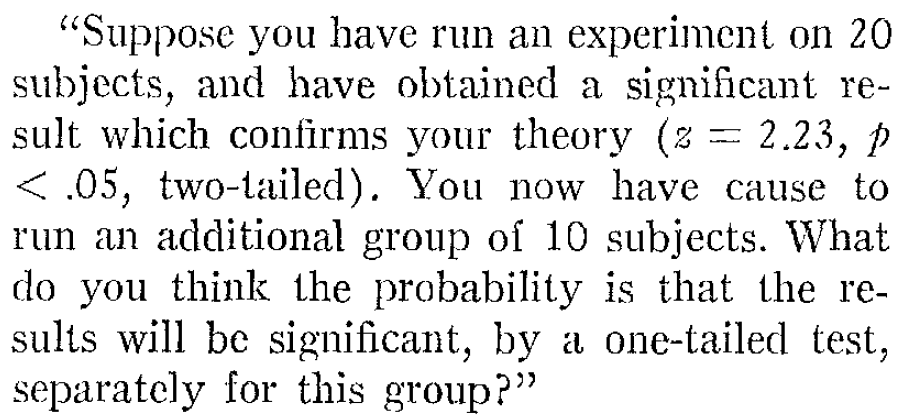
\includegraphics[width=1\textwidth,height=\textheight]{images/belieflawsmallnumers.png}

}

\caption{\label{fig-smallnumbers}Screenshot of first paragraph in
Tversky and Kahneman, 1971.}

\end{figure}

\begin{quote}
假设你对20名被试进行了实验,并得到了一个能证实你理论的重要结果(z=2.23,p\textless0.05,双尾)。你现在再做一组10人的实验,你认为这一组的结果通过单尾检验并具有统计学意义的概率是多少?
\end{quote}

Tversky和Kahneman认为合理的答案是48\%,但唯一的正确答案与问题9的正确答案相同,确切的概率无法得知(Miller,
2009)。

\textbf{问题10:} 一个不显著的p值(例如p = 0.65)是否意味着零假设为真?

\begin{enumerate}
\def\labelenumi{\Alph{enumi})}
\tightlist
\item
  不是,该结果可能是II类错误,或假阴性。
\item
  是的,因为该结果是一个真阴性。
\item
  是的,如果p值大于α水平,则零假设为真。
\item
  不是,因为你需要至少两个不显著的p值才能得出零假设是真的结论。
\end{enumerate}

\textbf{问题11:}
以下哪一个是采用了正确的方式来表达p值不显著(例如在独立t检验中使用0.05的α水平,p
= 0.34)?

\begin{enumerate}
\def\labelenumi{\Alph{enumi})}
\tightlist
\item
  零假设被证实,p \textgreater{} 0.05
\item
  两个条件之间没有差异,p \textgreater{} 0.05
\item
  观察到的差异在统计学上与0没有差异。
\item
  零假设为真。
\end{enumerate}

\textbf{问题12:} 观察到一个显著的p值(p \textless{}
0.05)是否意味着零假设是假的?

\begin{enumerate}
\def\labelenumi{\Alph{enumi})}
\tightlist
\item
  不,因为p\textless0.05只意味着备择假设是真的,而不是说零假设是错的。
\item
  不是,因为p值从来不是关于假设或理论的概率的声明。
\item
  是的,因为一个异常罕见的事件已经发生。
\item
  是的,因为差异在统计学上是显著的。
\end{enumerate}

\textbf{问题13:}
在统计学上有意义的效应是否总是意味着该效应在实践中也很重要?

\begin{enumerate}
\def\labelenumi{\Alph{enumi})}
\tightlist
\item
  不是,因为在超大样本中,极小的效应也可以有统计学意义,而小的效应在实际生活中从来就没有重要性。
\item
  不,因为理论上阿尔法水平可以设定为0.20,在这种情况下,显著的效应在实际生活中并不重要。
\item
  不是,因为一个效应有多重要取决于成本效益分析,而不是取决于在零假设下数据有多令人惊讶。
\item
  以上都是对的。
\end{enumerate}

\textbf{问题14:} 以下关于p值定义哪一个是正确的?

\begin{enumerate}
\def\labelenumi{\Alph{enumi})}
\tightlist
\item
  p值是指零假设为真的概率,意味着给定的数据与您观察到的数据一样极端或更极端。
\item
  p值是备择假设为真的概率,意味着给定的数据与您观察到的数据一样极端或更极端。
\item
  假设备择假设为真,p值是指观察到的数据与您观察到的数据一样极端或更极端的概率。
\item
  假设零假设为真,p值是指观察到的数据与您观察到的数据一样极端或更极端的概率。
\end{enumerate}

\hypertarget{ux5f00ux653eux6027ux95eeux9898}{%
\subsection{开放性问题}\label{ux5f00ux653eux6027ux95eeux9898}}

\begin{enumerate}
\def\labelenumi{\arabic{enumi}.}
\item
  什么决定了 p 值分布的形状?
\item
  当存在真实效应并且样本量增加时,p 值分布的形状如何变化?
\item
  什么是林德利悖论?
\item
  当真实效应不存在时,p 值如何分布?
\item
  p 值的正确定义是什么?
\item
  为什么不显著的 p 值意味着零假设为真是不正确的?
\item
  为什么显著的 p 值意味着零假设为假是不正确的?
\item
  为什么显著的 p 值意味着发现了在实际生活中重要的效应是不正确的?
\item
  如果您观察到重要发现,您犯第 1 类错误(假阳性)的概率是
  5\%,为什么这种观点是不正确的?
\item
  为什么1 - p(例如 1 -- 0.05 =
  0.95)并不是指在重复研究时效应也能被重复的概率?
\end{enumerate}

\bookmarksetup{startatroot}

\hypertarget{sec-power}{%
\chapter{论证样本量的合理性}\label{sec-power}}

在线版本: https://mp.weixin.qq.com/s/RBXptSamb3V9ZVF2vaijdQ

一般来说研究者进行实证研究,收集有助于回答研究问题的数据。所收集的数据越多,为研究问题所提供的信息量也就越大。对样本量合理性的论证应该以(统计)推断目标为基础,推断目标可能是估计效应量的大小,或者是检验一个假设。虽然在论文提交指南、基金申请、伦理审查等中,都会要求进行样本量合理性的论证,但是,观测数据的样本量大小通常只是被陈述出来,而非经过论证得出。这让我们难以评估研究的信息量。为了避免问题的发现为时太晚(例如,得到不显著的假设检验结果),研究人员应该在数据收集前仔细论证其样本量的合理性。

\hypertarget{tbl-table-pow-just}{}
\begin{longtable}[]{@{}ll@{}}
\caption{\label{tbl-table-pow-just}论证单个研究样本量合理性的方法概览}\tabularnewline
\toprule\noalign{}
论证的类型 & 适用情况 \\
\midrule\noalign{}
\endfirsthead
\toprule\noalign{}
论证的类型 & 适用情况 \\
\midrule\noalign{}
\endhead
\bottomrule\noalign{}
\endlastfoot
测量整个总体 &
研究者能够具体化总体的情况,总体本身是有限的,(几乎)每个个体都可被测量。 \\
资源受限 & 资源受限是限制研究者所能收集到的样本量的首要原因。 \\
精确度 &
研究问题关注某个参数的大小,研究者收集足够的数据使估计值达到想要的精确度。 \\
先验检验力分析 &
研究目的是检验能否以理想的统计检验力在统计学上拒绝某些效应量。 \\
直觉 &
研究者根据文献描述或口头交流中获得的直觉、一般规则或常规做法来决定样本量。 \\
不做论证 &
研究者没有为选择特定的样本量说明任何理由,或没有明确指定的推断目标,且没有诚实地表达这一点。 \\
\end{longtable}

\hypertarget{ux8bbaux8bc1ux6837ux672cux91cfux5408ux7406ux6027ux7684ux516dux79cdux65b9ux6cd5}{%
\section{论证样本量合理性的六种方法}\label{ux8bbaux8bc1ux6837ux672cux91cfux5408ux7406ux6027ux7684ux516dux79cdux65b9ux6cd5}}

研究者通常很难论证其样本量的合理性(样本指的是被试量、观察值的数量及两者的组合)。本综述将讨论六种可用来回答定量研究中这个问题的方法。本文不求面面俱到,但涵盖了单项研究所能用到的最常见且适用的方法。第一种论证样本量合理的方法,整个总体或者几乎整个总体的数据都被收集到了。第二种论证样本量合理的方法以资源有限为核心,资源有限是非常常见的,但很少明确地对其进行评估。第三种和第四种论证立足于研究者所期望的统计检验力或精确度。第五种论证则依赖于直觉,最后一种则是不做任何论证,直接选择一个样本量。以上每一种方法提供的合理性可强可弱,取决于研究者想要从计划采集的数据中推断出什么结论。

以上论证样本量合理性的方法------即使是''不做论证''的方法------都能让其他人了解到决定样本量大小的原因。显然,``直觉''和''不做论证''都不太可能给同行留下好印象。需要指出的是,这些论证的价值取决于我们从中获得了多少能够回答如下问题的信息:最终的样本量在多大程度上允许研究者进行他们预期的研究推断?也就是说,选择哪种具体的方法本身并不是关键。

上述论证方法在多大程度上能帮助研究者评估''数据''是否有信息,还取决于研究者在确定样本量时所提出的研究问题本身的细节及他们所选择的参数。一个非常差的先验统计检验力分析立刻会让研究变得只有非常低的信息量。当然,上述这六个论证方法并非互斥,设计一项研究时可以考虑多种方法并用。

\hypertarget{ux516dux79cdux65b9ux6cd5ux8bc4ux4f30ux54eaux4e9bux6548ux5e94ux91cfux503cux5f97ux5173ux6ce8}{%
\section{六种方法,评估哪些效应量值得关注}\label{ux516dux79cdux65b9ux6cd5ux8bc4ux4f30ux54eaux4e9bux6548ux5e94ux91cfux503cux5f97ux5173ux6ce8}}

我们收集的数据包含多大的信息量,这取决于研究者或同行(在某些情况下)所设定的推断目标。本文所考虑的各种不同的推断目标都有一个共同点,那就是研究者需要辨别出哪些效应量是有意义的。这也就意味着研究者需要对这些效应量进行评估。评估方式依赖于(某些方法的)统计特性以及某领域知识之间的相互结合。表2提供了六种可能的评估方式。但本文并不是要做一个全面介绍,而是提供一些易上手、常见且实用的方式。需要说明的是,这些评估方式并不是都与样本量的论证相关。由于这些评估都依赖相同的信息(如效应量、观察次数、标准差等),因此这六种评估方式可被视为一套互补的方法,来用于评估哪些效应量是值得引起关注的。本文附带的在线应用程序为广大研究者提供了一个可交互的表格,希望能够指导研究者完成样本量论证时需要注意的事项。

首先,研究者应当考虑他们所感兴趣的最小效应量是多少。第二,尽管这只与假设检验相关,研究者仍应当考虑哪些效应量会在统计上显著(在既定的显著性水平
\(\alpha\)
和样本量之下)。第三,重要的是考虑预期效应量的范围,这需要思量预期效应的来源以及其中可能存在的偏差。第四,围绕总体可能的效应量来设置置信区间的宽度是有益的,因为我们可能需要用置信区间来拒绝其他可能的效应。第五,在做灵敏度功效分析时,应当广泛地估量潜在效应量的统计检验力。第六,应当考虑已发表的相关研究中效应量分布。

\hypertarget{tbl-table-effect-eval}{}
\begin{table}
\caption{\label{tbl-table-effect-eval}评估哪些效应量值得关注的方法概览 }\tabularnewline

\centering
\begin{tabular}{>{\raggedright\arraybackslash}p{5cm}|>{\raggedright\arraybackslash}p{10cm}}
\hline
评估方式 & 研究者所面临的问题\\
\hline
感兴趣的最小效应量 & 从理论或实践层面上来说,有意义的最小效应量是多少?\\
\hline
统计上可得的最小效应量 & 给定测量方式和样本量,达到统计显著的临界效应量是多少?\\
\hline
预期效应量 & 根据理论预测或前人的研究,预期的效应量是多少?\\
\hline
置信区间宽度 & 在围绕着效应量设立置信区间时,有哪些效应量应当被排除在外?\\
\hline
灵敏度功效分析 & 在一系列潜在的效应量中,哪种效应在进行假设检验时最敏感?\\
\hline
某研究领域的效应量分布 & 在某个特定的研究领域,效应量的一般范围是多少?哪些效应是本来就不太可能被观察到的?\\
\hline
\end{tabular}
\end{table}

\hypertarget{ux4fe1ux606fux4ef7ux503c}{%
\section{信息价值}\label{ux4fe1ux606fux4ef7ux503c}}

几乎所有研究者都会面临资源的限制,因此他们需要在成本(收集额外数据的花费)与效益(额外数据所带来的的价值)之间进行权衡。通常,这被称为''信息价值''\emph{value
of information}, (Eckermann et al.,
2010)。然而,衡量信息价值是极其困难的(Detsky,
1990)。研究者不仅需要明确收集数据所需的成本,还需要去权衡这些成本所带来的收益。从信息价值的角度来看,并不是每个可收集的数据都具有同等的价值(J.
Halpern et al., 2001; Wilson,
2015)。每当额外的数据并没有为推断目标提供更多的价值时,那么所花费的成本就会超过所需收益。

在大多数情况下,额外的信息(数据)并不止是发挥单一的作用,尤其是涉及多个推论目标时。研究者可能希望将某一效应与前人研究中所发现的大效应量或者基于理论预测得出的中等效应量以及具有实践意义的最小效应分别进行比较。在这种情况下,由于样本信息的价值差异,因此将导致每个推理目标的最佳样本量不同。在研究中,收集关于某个大效应量的数据信息是非常有价值的,随着数据的增加,额外数据的边际效益逐渐减少,甚至可能变为负值。然而,针对中等效应量的信息价值来说,继续收集数据到一定程度,额外数据的信息价值再次增加。对于较小效应量的信息价值来说,随着数据继续增加,会再次出现边际效益递减的情况,直到研究收集的数据越来越能够提供有关最小效应大小是否存在的信息价值(如果效应不存在,收集更多的数据也是无意义的)。

由于难以量化信息的价值,研究者在研究中通常使用不够规范的方式来证明他们样本量的合理性。尽管成本-效益分析在报告样本量合理性时总是模棱两可的,但信息价值的观点几乎隐含在所有论证样本量的理论框架中。故在随后对样本量论证的讨论中,我们将反复强调在(统计)推断目标下信息价值的重要性。

\hypertarget{ux6d4bux91cfux51e0ux4e4eux603bux4f53ux6570ux636e}{%
\section{测量(几乎)总体数据}\label{ux6d4bux91cfux51e0ux4e4eux603bux4f53ux6570ux636e}}

在某些情况下,有可能会从总体收集全部(几乎)数据。例如,研究者可能会使用人口普查数据库,来收集某公司所有职工的数据,或者研究一小部分顶尖运动员。只要有可能测量总体,样本量论证的缘由就变得直截了当,因为研究者获得了所有可用的数据。

当测量总体时,就不需要进行假设检验了。毕竟,此时不存在可推论的群体{[}2{]}。当收集了总体数据后,那么总体的效应量就已知了,且不需要计算置信区间。如果总体规模已知,但并未测量全部的数据,那么随着被试量逐渐趋近于目标总体,置信区间宽度也将逐渐缩小到零。这被称为估计方差的有限总体校正系数(Kish,
1965)。样本均值的方差为
,而在有限总体中,它要乘以标准误的有限总体校正系数:

其中 N 为总体大小, n 为样本量。当 N 远大于 n
时,校正系数将趋近于1(因此,当总体非常大时,这种校正通常被忽略,尽管总体是有限的),并且不会对方差产生显著影响。当测量总体时,校正系数为
0 ,这样方差也为 0 。例如,当总体为 100 名顶尖运动员时,采集的样本量为
35 名运动员,有限总体校正系数为 。superb
R包可以计算校正后的总体置信区间(Cousineau \& Chiasson, 2019)。

\hypertarget{ux6709ux9650ux7684ux8d44ux6e90}{%
\section{有限的资源}\label{ux6709ux9650ux7684ux8d44ux6e90}}

在研究中,常因资源限制而使得数据无法合理收集(Lenth,
2001)。因此实际上,样本量总是受到资源的限制,纵使它并不是决定样本量的主要缘由,但也总是次要缘由。

尽管资源限制无处不在,但样本量的问题在实验设计环节却没有得到足够的重视(一个例外的例子,可见
Bulus \& Dong
(2021)。这导致人们觉得承认资源限制是不合时宜的,但事实并非如此,资源限制是一个很常见的问题,所以一个负责任的研究者在设计研究时,应当仔细评估资源限制所带来的影响。同样的,资源限制的评估也是数据收集的成本与数据信息价值之间的权衡。即使研究者没有明确量化这种权衡,但这也会在他们的实际操作中体现出来。例如,研究者很少把所有的资源都投在某一项研究上。鉴于资源有限,研究者们面临的是如何在多个研究项目上优化资源的分配。

时间和经费是所有研究者都要面临的限制。一个博士生有一定的时间来完成一篇博士论文,但通常在这段时间内也需完成多条研究线。除了时间限制,研究者的经费也很有限,这往往直接影响到数据收集的数量。在某些研究领域也存在的第三种限制,比如在研究患有罕见疾病的患者时,可能本身能够获取的数据量就非常少。总而言之,将有限资源的优化置于规划样本量的首要位置,并从研究者的可用资源出发。将其在既定的时间、成本内转化为研究者预期的样本量(N)。但问题就在于如何评估这N个测量值是否值得。如何判断一项研究是否提供了充足的信息,以及判断数据收集从何时起将没有意义?

当衡量资源受限是否使数据收集信息不足时,研究者需要明确他们在收集数据时的推断目标是什么(Parker
\& Berman,
2003)。但有数据总比没有数据强,所以从某种意义上来说,所有收集到的数据都是有价值的。然而,收集数据所花费的成本可能超过了数据所带来的价值。

无论有或没有数据,在确实需要做出决策时,对数据收集是否具有价值进行评估是最直接的方法。在这种情况下,任何额外的数据都将减少决策过程的错误率,哪怕只是一点点。例如,在没有数据的情况下,让我们猜测两种条件中哪个条件的真实平均分数更高,显然我们的猜测不会比猜抛硬币来的更加准确。但有了一些数据后,我们可以选择具有更高平均值的条件,并以此做出更准确的决策。尽管拥有少量的数据,但我们仍可能犯错误,但错误率比没有任何数据要小。在这些情况下,只要错误率的降低优于数据收集的成本,那么信息价值可能便是正向的。

小样本数据体现价值的另一种方式是,它可能将会被用来进行元分析(Maxwell \&
Kelley,
2011)。这种方式需小样本满足以下要求:1)研究者需公开数据,使得这些数据可用于日后的元分析;2)这些数据在未来有相当大的概率可被用于一个高质量的元分析(S.
D. Halpern et al.,
2002)。然而,关于未来是否会有这样的元分析是不确定的,所以需要将这种不确定性与数据收集的成本进行权衡。

提高未来元分析可能性的一种方法是,由研究者自己来进行,他们可将进行的几项研究融合成一个小规模的元分析中(Cumming,
2014)。例如,研究者可能计划在接下来12年的授课中重复一项研究,并期望在12年后,对这12项研究进行元分析来求得有效推论(参考
ter Schure \& Grünwald
(2019))。此外,如果一个研究者无法自己收集所需数据,他们也可以尝试建立一个合作网,让同一领域内的其他研究者使用相同方法收集类似的数据。如果随着时间的推移,仍然不可能出现足够的数据来证实推断目标,那么对数据的收集就毫无意义。

即使研究者认为收集数据是有意义的,因为将来会进行元分析,同样他们也很可能会对当前数据进行统计分析。为了确保他们对分析结果的预期是准确的,首要考虑哪些效应量是有趣的,并进行灵敏度功效分析,以此估计感兴趣的效应出现
Ⅱ
类错误的概率。我们可从六个方面来评估效应量的意义,稍后会在本文的第二部分进行讨论。我们需要斟酌能达到统计显著的最小效应量,围绕效应量的置信区间可能的宽度,以及在特定领域中可预期的效应。并在灵敏度功效分析中评估以上效应的统计功效。如果已经确定好了研究问题,那么可以考虑使用折中检验力分析来确定合适的错误率。

对资源受限的样本量估计进行阐述时,建议先从表
Table~\ref{tbl-table-pow-rec}
中提到的五个因素入手。明确地解决这些问题有助于评估数据是否值得收集。为了清晰地解决所有相关问题,可以在
https://shiny.ieis.tue.nl/sample\_size\_justification
找到一个交互式表格来进行。

\hypertarget{tbl-table-pow-rec}{}
\begin{table}
\caption{\label{tbl-table-pow-rec}Overview of recommendations when reporting a sample size justification
based on resource constraints. }\tabularnewline

\centering
\begin{tabular}{>{\raggedright\arraybackslash}p{5cm}|>{\raggedright\arraybackslash}p{10cm}}
\hline
需要解决什么? & 怎么来解决?\\
\hline
日后是否会有相关的元分析? & 考虑到未来可能会有相当多的类似研究出现,这就使元分析变得更有可能实现。\\
\hline
是否会考虑在现有数据(不论其是否可用)的情况下做出结论? & 如果做出了决策,那么收集的任何数据都将降低错误率。需考虑使用折中检验力分析来确定 I 类和 II 类错误的错误率。为了降低错误率所付出的代价值得吗?\\
\hline
临界效应量是多少? & 报告和解释临界效应量的大小,重点关注预期的效应量是否能产生显著的结果。如果不能,则表明对数据的解释将不能拘泥于 p 值。\\
\hline
置信区间的宽度是多少? & 报告并解释置信区间的宽度。有这样不确定性的估计会有怎样的作用?如果零假设为真,那么拒绝置信区间外的效应是否值得(忽略低统计检验力的实验设计可能导致无法拒绝这些效应的情况)?\\
\hline
哪些效应量有良好的统计检验力? & 报告灵敏度功效分析,并报告期望检验力水平范围内(例如,80\%、90\%和95\%)可以检测到的效应量大小,或绘制灵敏度分析图。\\
\hline
\end{tabular}
\end{table}

\hypertarget{sec-aprioripower}{%
\section{先验检验力分析}\label{sec-aprioripower}}

若一项研究以是否存在统计学意义上的显著为目标时,研究者往往希望确保他们的样本量足够大,以免对他们所关心的效应量做出错误结论。在上述论证样本量合理性的方式中,信息价值在于收集数据,从长远来说,可以收集数据直到得出错误结论的概率小于一个期望值。此时,如果研究者进行假设检验,有四种可能的结果:

\begin{enumerate}
\def\labelenumi{\arabic{enumi}.}
\tightlist
\item
  假阳性( I 类错误),由 \(\alpha\)
  水平决定。即使零假设为真,也会得到显著结果。
\item
  假阴性( II 类错误),由 \(\beta\) ,或 1-power
  决定。即使备择假设为真,也会得到不显著的结果。
\item
  真阴性,由 1-\(\alpha\) 决定。当零假设为真时,得到不显著的结果。
\item
  真阳性,由 1-\(\beta\) 决定。当备择假设为真时,得到显著的结果。
\end{enumerate}

在既定的效应量、 \(\alpha\)
水平和统计检验力下,可以使用先验检验力分析来计算某一效应{[}3{]}所需要的样本量(在期望错误率之下)。图
Figure~\ref{fig-power-2} 给出了在双侧 \(\alpha\) 水平为 0.05 的独立 t
检验中,统计检验力如何随着样本量(每组)的增加而增加。如果我们对 d = 0.5
的效应感兴趣,则每个条件下 90 的样本量将为我们提供超过 90\%
的统计检验力。可以用统计检验力来确定被试的数量或项目的数量(Westfall et
al., 2014),同样也可以通过单个案例研究进行计算(Ferron \& Onghena, 1996;
McIntosh \& Rittmo, 2021)。

尽管普遍将 I 类错误设为 5\% 、统计检验力设为 80\%
,但它们的设定应该是有理有据的(Lakens, Adolfi, et al.,
2018)。如''折中检验力分析''部分所述,默认 80\%
的统计检验力也缺乏依据。一般来说,错误率越低(从而统计检验力越高),研究的信息量越大,但需要的资源也就越多。在想要达到
90\% 或 95\%
检验力的研究中,研究者应考虑样本量的成本与降低错误率的收益之间的关系。除此之外,研究者还应考虑是否计划发表一篇由重复和拓展以往研究而构成的文章,在这种情况下,观察到多个
I
类错误的概率将非常低,但即使存在真实效应,得到混淆结果的概率也会增加(Lakens
\& Etz, 2017),这也是研究 II
类错误低的一个原因,鉴于此,或许可以稍微提高每个单项研究的 \(\alpha\)
水平。

\begin{figure}

{\centering 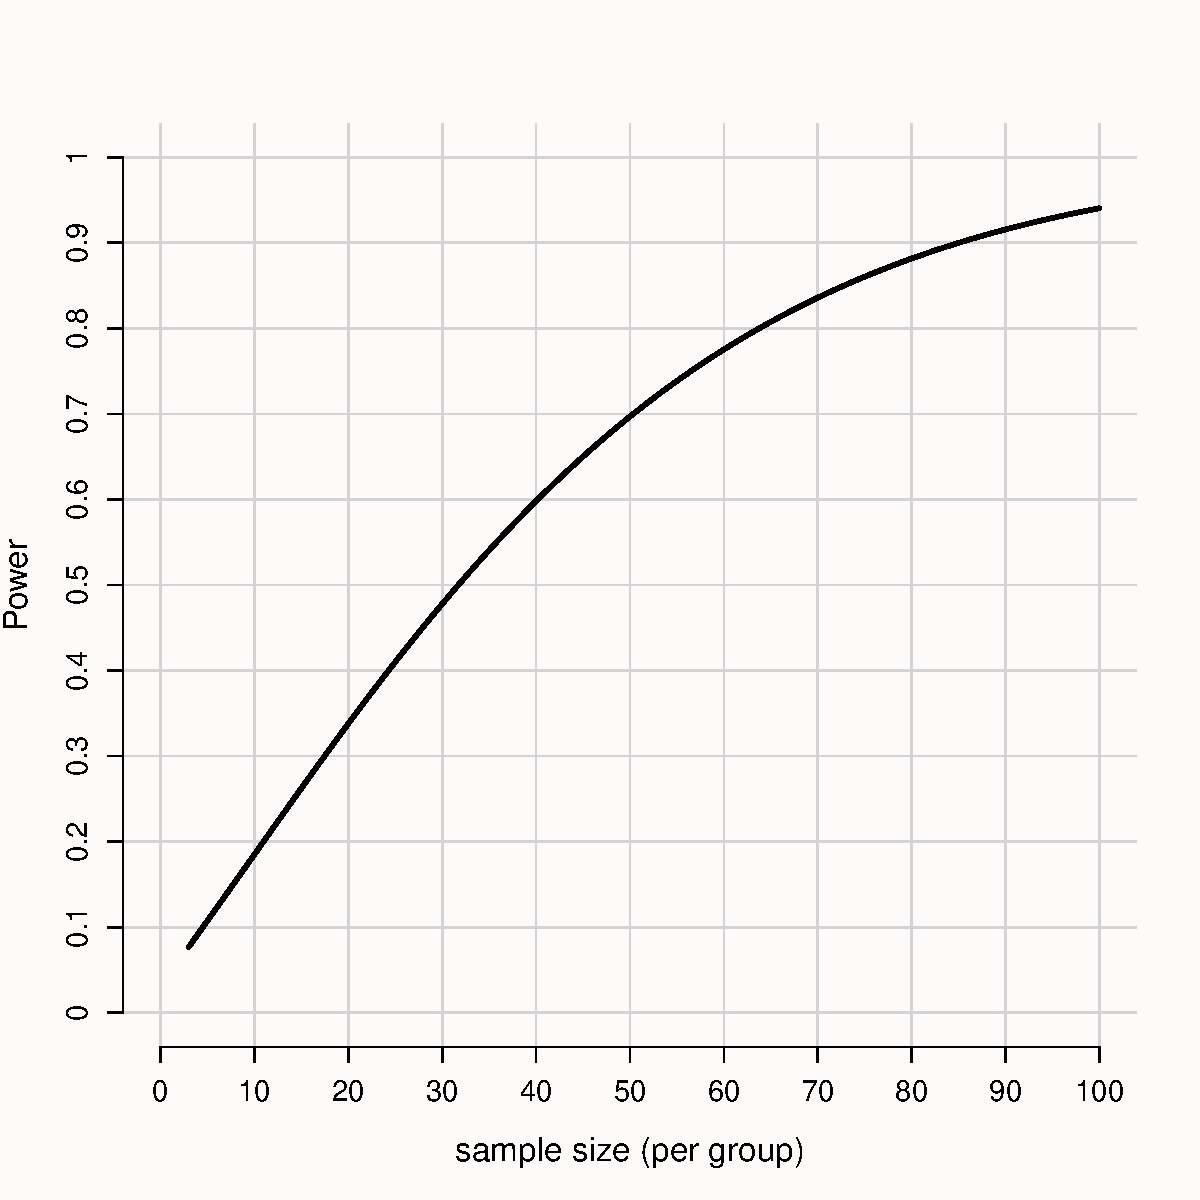
\includegraphics[width=1\textwidth,height=\textheight]{08-samplesizejustification_files/figure-pdf/fig-power-2-1.pdf}

}

\caption{\label{fig-power-2}效应 d = 0.5, \(lpha\) = 0.05 的独立 t
检验的统计检验力曲线与样本量的关系}

\end{figure}

Figure~\ref{fig-power-3} 呈现了两个分布。左边的分布(灰色虚线)以 0
为中心。这是零假设的模型。如果此时零假设为真,那么只有在极端效应量的情况下(在正向或负向的双侧检验中)会得到统计意义上显著的结果,但所有显著结果都犯了
I
类错误(曲线下深灰色的区域)。如果效应不存在,则零假设显著检验的统计检验力是不确定的。也就是说,在既定的
\(\alpha\) 水平下,如果零假设为真,任何所得显著结果都是 I
类错误或假阳性。右边的分布(黑色实线)以 d = 0.5
的效应为中心。这是备择假设的模型,说明如果备择假设为真时,预期效应量为 d
= 0.5
。但是即使存在真正的效应,研究也不一定能得到具有统计学意义上的显著结果。由于变异具有随机性,所得效应量接近于0而不具有统计学意义时,就会发生这种情况。这样的结果是假阴性(右侧曲线下方的浅灰色区域)。为了提高检验力,我们可以增加样本量。随着样本量的增加,分布变得更窄,从而降低了发生
II 类错误
的概率。上述图片可以在一个在线应用程序中进行复刻和调整:http://shiny.ieis.tue.nl/d\_p\_power/

\begin{figure}

{\centering 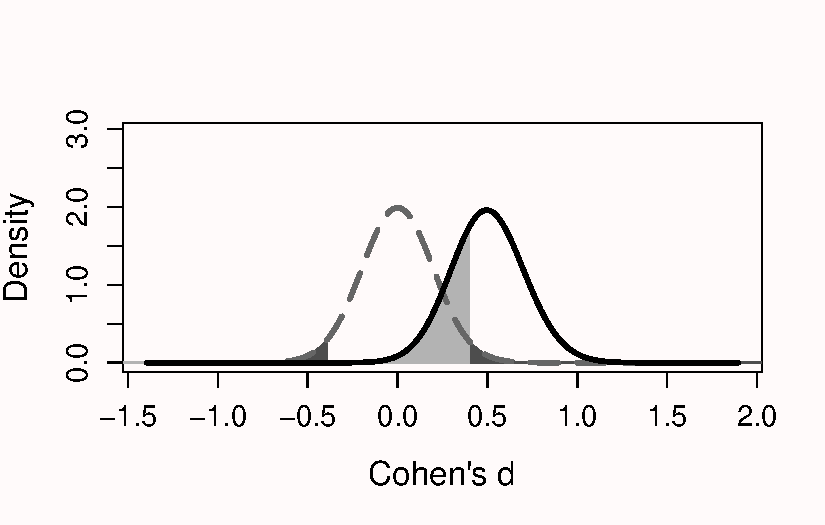
\includegraphics[width=1\textwidth,height=\textheight]{08-samplesizejustification_files/figure-pdf/fig-power-3-1.pdf}

}

\caption{\label{fig-power-3}零假设(d = 0,灰色虚线)和备择假设(d =
0.5,黑色实线),且\(lpha\) = 0.05,n = 80每组}

\end{figure}

需要强调的是,先验检验力分析的目的并不是为真实效应提供足够的统计检验力。真实的效应量是未知的。先验检验力分析的目的是,在研究者想要探究特定的效应量(小、中、大)时,能够获得足够的统计检验力。就像
I 类错误是在零假设为真的条件下发生 I
类错误的最大概率一样,先验检验力分析是假设在特定效应量下进行计算的。且这个假设正确与否不得而知。研究者所能做的就是确保他们的假设是合理的。研究(对
II
类错误进行控制)的统计推断是以特定效应量的假设为基础的。他们允许推断,假设真实效应量至少与先验检验力分析中使用的一样大,则研究中的最大
II 类错误率不高于先前的期望值。

如果在研究时,我们对''有''效应和''无''效应都进行了先验检验力分析,也许就能更好的进行说明。在设计研究时,必须考虑无效应的可能性(例如,平均值的差异为零)。先验检验力分析既可以用于零假设显著性检验,也可以用于零效应的检验,例如等价检验,可以通过拒绝''有''效应来为零假设提供统计学上的支持(Lakens,
2017; Meyners, 2012; J. L. Rogers et al.,
1993)。当对同一样本进行多个预实验时,每次分析都需要独立的对样本量进行论证。如果可能的话,要确保收集的样本量(每次)为所有实验提供信息,也就是说,收集的样本量是基于全部先验检验力分析所得到的最大样本量。

例如,如果一项研究是以 90\% 的统计检验力来接受或拒绝 d = 0.4
的效应,并且将双侧独立 t 检验的 \(\alpha\) 水平定为 0.05
,则研究者需要在每个条件下收集 133 个被试进行假设检验,以及每个条件 136
个被试进行等价检验。因此,研究者应争取收集 272
名被试进行两种检验来更好的做出结论。但这并不能保证某研究具有足够的统计检验力来获取真实效应(永远无法得知),但它保证了研究者具有足够的统计检验力来接受或拒绝关于某效应的假设。因此,只要研究者能够证明他们感兴趣的效应量是合理的,先验检验力分析就是有用的。

如果研究者在检验多个假设时矫正了 \(\alpha\)
水平,则先验检验力分析应基于矫正后的 \(\alpha\)
水平。例如,如果进行了四次检验, I 类错误率为 5\%
,进行Bonferroni校正后,则先验检验力分析应基于 0.0125 的校正 \(\alpha\)
水平。

先验检验力分析可以通过分析法或计算模拟来进行。分析法速度更快,但灵活性较差。当研究者试图对更复杂的或不常见的检验方法进行统计检验分析时,他们将面临的一个共同挑战是,当前软件不能提供现成的解决方案。在这种情况下,计算模拟可以为任何检验方法提供一个灵活的解决方案(Morris
et al., 2019)。以下代码是在R语言中进行计算模拟的示例,它对样本量为 20
的单样本 t 检验进行了 10000 次模拟迭代,此时假设真实的效应量为 d = 0.5
。所有的模拟都由给定规则的随机数据组成(例如,均值为 0.5 、标准差为 1
的正态分布),然后对数据进行检验。通过计算显著结果的百分比,就能算出任何检验方法的统计检验力。

\begin{Shaded}
\begin{Highlighting}[]
\NormalTok{p }\OtherTok{\textless{}{-}} \FunctionTok{numeric}\NormalTok{(}\DecValTok{10000}\NormalTok{)   }\CommentTok{\# to store p{-}values}
\ControlFlowTok{for}\NormalTok{ (i }\ControlFlowTok{in} \DecValTok{1}\SpecialCharTok{:}\DecValTok{10000}\NormalTok{) \{  }\CommentTok{\# simulate 10k tests}
\NormalTok{  x }\OtherTok{\textless{}{-}} \FunctionTok{rnorm}\NormalTok{(}\AttributeTok{n =} \DecValTok{20}\NormalTok{, }\AttributeTok{mean =} \FloatTok{0.5}\NormalTok{, }\AttributeTok{sd =} \DecValTok{1}\NormalTok{)}
\NormalTok{  p[i] }\OtherTok{\textless{}{-}} \FunctionTok{t.test}\NormalTok{(x)}\SpecialCharTok{$}\NormalTok{p.value }\CommentTok{\# store p{-}value}
\NormalTok{\}}
\FunctionTok{sum}\NormalTok{(p }\SpecialCharTok{\textless{}} \FloatTok{0.05}\NormalTok{) }\SpecialCharTok{/} \DecValTok{10000} \CommentTok{\# Compute power}
\end{Highlighting}
\end{Shaded}

有各种各样的工具都能用来统计检验力分析。无论研究者决定使用哪种工具,都需要时间来学习如何正确使用该软件,再进行有意义的先验检验力分析。针对心理学领域进行检验力分析的教学资源非常丰富(Aberson,
2019; Cohen, 1988; Julious, 2004; Murphy et al.,
2014),例如,有概括性的介绍(Baguley, 2004; Brysbaert, 2019; Faul et al.,
2007; Maxwell et al., 2008; Perugini et al.,
2018),以及现在越来越多的关于特定检验的实用教程(Brysbaert \& Stevens,
2018; DeBruine \& Barr, 2021; P. Green \& MacLeod, 2016; Kruschke, 2013;
Lakens \& Caldwell, 2021; Schoemann et al., 2017; Westfall et al.,
2014)。学习统计检验力相关的基础知识非常重要,对学会如何执行基于计算模拟的检验力分析也大有裨益。我们也建议寻求专家的帮助,特别是当研究者对某特定检验的统计检验力分析缺乏经验时。

报告先验检验力分析时,请确保统计检验力分析是完全可重复的。如果在R中进行统计检验力分析,则可以共享分析脚本和相关包版本的信息。在许多软件中,可以直接将统计检验力分析导出为
PDF 文件。例如,可以在G*Power的''protocol of power
analysis''选项下导出分析。如果软件没有提供导出的方法,请在补充文件中提供统计检验力分析的截图。

\begin{figure}

{\centering 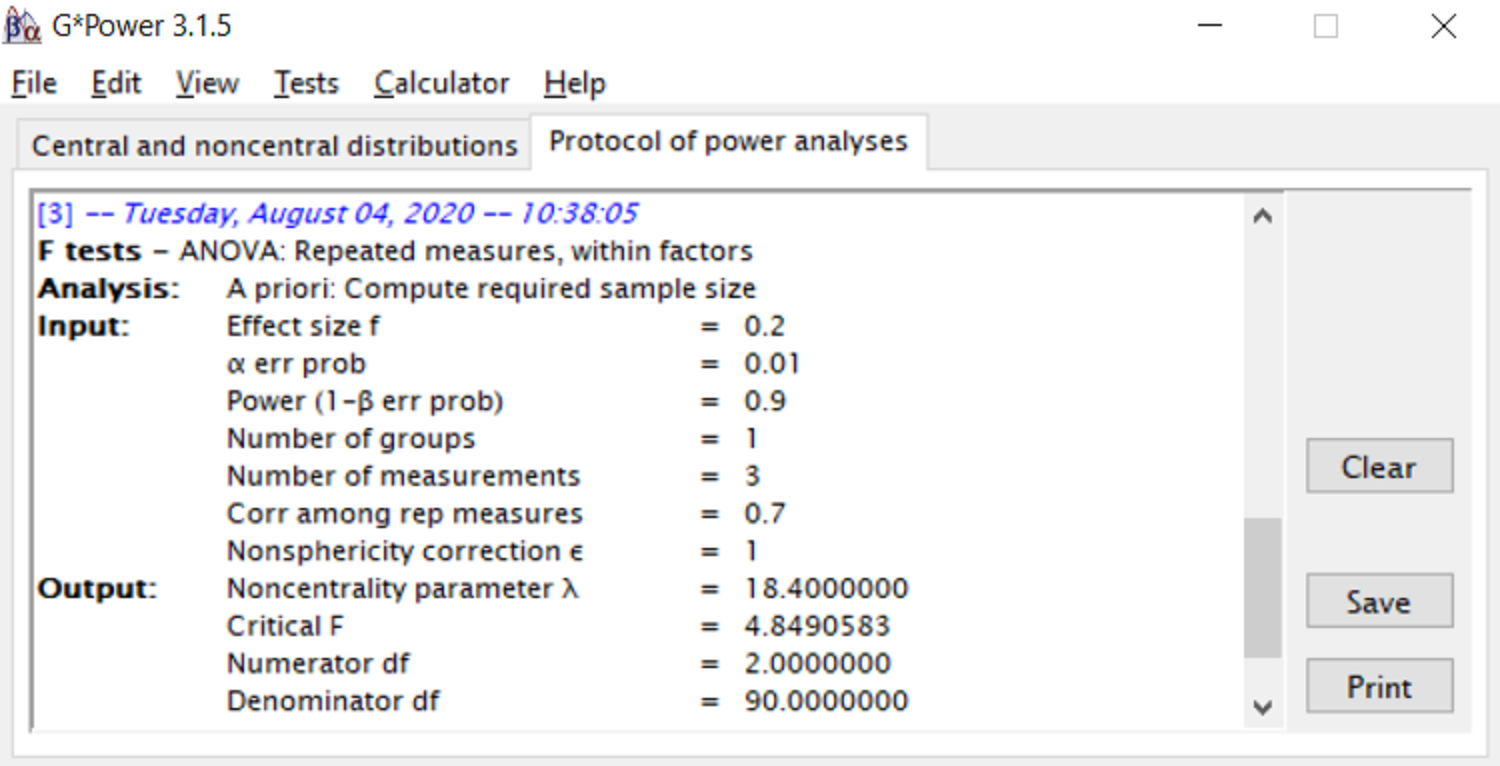
\includegraphics[width=1\textwidth,height=\textheight]{images/gpowprotocol.png}

}

\caption{\label{fig-gpowprotocol}关于统计检验力分析的所有细节都可以在G*Power中导出}

\end{figure}

有关可重复性的报告中需要附上参数选择的理由。如果检验力分析中使用的效应量是基于前人的研究,可依据表
Table~\ref{tbl-tablemetajust}(如果效应是基于元分析)或表
Table~\ref{tbl-table-es-just}(如果效应是基于单项研究)中的观点进行探讨。如果效应量的估计基于现有文献,还请提供完整的引文,最好是直接引用进行样本量论证的文章。如果效应量是基于感兴趣的最小效应量,则不仅需要说明该值,还需证明该值是合理的(例如,基于理论预测或实践意义,请参见
Lakens, Scheel, et al.
(2018)。有关先验检验力分析时应报告的所有方面,请参考表
Table~\ref{tbl-table-pow-rec-2}。

\hypertarget{tbl-table-pow-rec-2}{}
\begin{table}
\caption{\label{tbl-table-pow-rec-2}报告先验检验力分析时的建议 }\tabularnewline

\centering
\begin{tabular}{>{\raggedright\arraybackslash}p{5cm}|>{\raggedright\arraybackslash}p{10cm}}
\hline
需要参考的事项? & 需要怎么做?\\
\hline
列出计划进行的主要检验 & 对检验进行说明,且指明需要控制 I 类和 II 类错误。\\
\hline
明确 \$lpha\$ 水平 & 列出每个检验的 I 类错误并说明理由。确保在必要时对多重比较进行校正。\\
\hline
期望的统计检验力是多少? & 列出每个检验的期望统计检验力(或者 II 类错误)并说明理由。\\
\hline
对于每一个检验力分析,要说明效应量类型,效应量大小以及针对该效应量进行检验力的理由 & 报告效应量类型(如Cohen's d, Cohen's f),效应量大小(如 0.3 ),选取该效应量的理由,以及是基于感兴趣的最小效应量、元分析估计的效应量还是以往单项研究估计的效应量,或其他来源。\\
\hline
考虑零假设为真的可能性 & 进行统计检验力分析,以考察是否存在有意义的效应(例如,等价检验的统计检验力)。\\
\hline
确保统计检验力分析是可重复的 & 包括用于统计检验力分析的代码,或导出一份统计检验力分析的详细报告。\\
\hline
\end{tabular}
\end{table}

\hypertarget{planprecision}{%
\section{规划精确度}\label{planprecision}}

一些研究者建议根据所需的估计精确度水平来论证样本量的合理性(Cumming \&
Calin-Jageman, 2016; Kruschke, 2018; Maxwell et al.,
2008)。基于精确度来论证样本量合理性时,其目的是得到围绕参数估计置信区间的宽度。参数估计的置信区间宽度取决于标准差和数据量。研究者根据精确度来论证样本量合理性时,唯一需要论证清楚的是与推理目标相关的置信区间的理想宽度,以及他们对总体标准偏差的假设。

如果研究者已经确定了所需的精确度,并且对真实的标准偏差有个很好的估计,则可以直接依据精确度水平计算所需的样本量。例如,在测量一组被试的IQ时,从长远来看,研究者可能希望用围绕均值2个标准差之内的
95\%
的数据来估计智商分数。达到这种精确度水平(假设数据呈正态分布)所需的样本量可以通过下式计算:

\[N = \left(\frac{z \cdot sd}{error}\right)^2\]

其中 N 是观察次数(样本量), z 是与所需置信区间相关的临界值,sd 是总体
IQ
的标准差,error是在期望错误率下,均值应落入的置信区间的宽度。在本例中,(1.96
× 15 / 2)\^{}2 = 216.1 个观测值。如果研究者希望有 95\%
的数据落在真实总体均值 2 个误差范围内,则应收集 217
个观测值(样本)。如果计算出非零均值差异(non-zero mean
difference)的所需精度,则精度是非中心的 t
分布。对于这些计算,需要对期望效应量进行估计,但对所需样本量的影响相对较小(Maxwell
et al.,
2008)。也可以将效应量的不确定性纳入样本量的计算中,这可称为''万全之策''(assurance)(Kelley
\& Rausch, 2006)。R中MBESS包提供了各种函数来估计检验的样本量(Kelley,
2007)。

但模棱两可的是所需的精确度水平与推理目标之间关系。没有任何文献可以帮助研究者选择所需的置信区间宽度。Morey
(2020)
说,大多数规划精确度的实例中都涉及到将所得效应与其他效应区分开的推断目标(关于贝叶斯观点,请参阅
Kruschke (2018)。例如,研究者可能期望 r = 0.4
的效应量,并会以不同的方式处理其相关性差异超出 0.2 的情况(因为0.2
\textless{} r \textless{} 0.6),因为 r = 0.6
或更大的效应也将会认为太大了,不可能是由假设的实验操纵所带来的(Hilgard,
2021),而小于 r = 0.2
的效应又被认为太小,从而无法支持理论预测。如果目标确实是为了获得一个足够精确的效应量估计,以便高概率的区分上述两种效应,那么推理目标实际上就是假设检验,
这就需要设计一个具有足够统计检验力的研究来拒绝效应(例如,检验相关性在
0.2 到 0.6 之间的预测范围)。

如果研究者不想检验假设,例如,可能他们更喜欢估计的方法而不是检验的方法,那么在没有明确的指导方针来帮助研究者确立精确度水平时,一种可行的方案可能是参照一个公认的精确度标准。该标准可能基于某一明确惯例(certain
resolution),低于该惯例时,某研究领域中的测量将不再有差异性的结果。正如研究者通常使用
0.05 的 \(\alpha\)
水平一样,他们可以对研究进行规划,在遵循惯例之下,得到期望效应的置信区间的理想宽度。那么未来的工作就是需要帮助研究者合理规划精确度置信区间的理想宽度。

\hypertarget{ux4ee5ux7ecfux9a8cux6cd5ux5219ux6765ux786eux5b9aux6837ux672cux91cfheuristics}{%
\section{以经验法则来确定样本量(Heuristics)}\label{ux4ee5ux7ecfux9a8cux6cd5ux5219ux6765ux786eux5b9aux6837ux672cux91cfheuristics}}

当研究者采用经验法则来确定样本量时,他们可能是因为自己无法评估样本量是否合理,但他们倾向于相信权威机构推荐的样本量。当我在2005年开始攻读博士时,大家通常会在每个条件下收集15名被试。当被问及为什么这么做时,没有人可以给出确切的答案,但人们相信这一做法在某篇文献中进行了合理的解释。但现在我意识到我们使用这样约定俗成的标准其实是没有任何的理论基础的。正如伯克利
(1735)
所说的:``人们从他人那里学习科研方法(准则):每个学习者或多或少都会对权威有所敬畏,尤其是年轻的学习者,很少有人愿意在这些原则性的问题上纠结很久,而是倾向于遵循原则:从某种程度上来说,早期被承认且又经过重复的东西会变得具有说服力:这种''说服力''最终变为了''证据''。

关于样本量的选择,一些文章为研究者提供了一些简单的经验法则。这类文章显然满足了人们的需求,并且被大量引用,即使这些文章中提供的建议存在纰漏。例如,Wilson
VanVoorhis \& Morgan (2007) 将 S. B. Green (1991) 提出收集约 50
个观测值的经验法则进行了修改,改为建议在回归分析中至少使用 50 + 8
个观测值。实际上,Green在他的文章中总结道:``总的来说,没有具体理论支持最小样本量或具有预测性的被试的subjects-of-predicotrs最小比率。''他在文中确实探讨了
N = 50 + 8
这一经验法则如何为社会科学中的''典型''研究提供具体的最小观测量(样本量),因为这些研究具有''中等''效应量,正如Green引用Cohen
(1998)所提及的那样。但实际上Cohen并没有声称典型的社科研究具有''中等''效应大小,而是说(1988,第13页):``许多在人格、社会和临床心理学研究中寻求的效应很可能是这里定义的小效应。''现在我们可看到一连串错误的引用最终是如何创造了一个具有误导性的经验法则。

经验法则似乎主要源于错误的引用和/或过分简化的建议。Simonsohn、Nelson和Simmons
(2011)建议''作者必须对于每个条件收集至少20个观察值。``后来,同一作者在一次会议上提出了
n \textgreater{} 50 的建议,除非你研究大的效应(Simmons et al.,
2013)。遗憾的是,这一建议现在经常被错误地引用来解释在不考虑预期效应量的情况下,每个条件下不超过
50
个被试的理由。如果作者根据另一篇论文中的一般性建议来论证某个样本量(例如,
n = 50
)的合理性,则可能是他们错误引用了该文章,或者他们引用的文章本身存在缺陷。

另一个常见的经验法则的方式是收集和前人研究相同的样本量。但有以下情况时,不建议采用这种方法,即在某领域普遍存在发表偏差时,或者主要是探索性的单项研究有新颖发现时。这种方法只有一种适用情况,那就是前人研究选取样本量的缘由也适用于当前的研究,这样的使用方法才是有效的。与其说你打算收集与前人研究相同的被试量,不如重复论证样本量的合理性,然后根据新发现进行更新(与前人研究的效应量讨论类似,见表
Table~\ref{tbl-table-es-just})。

同行评审和编辑应该仔细审查采用经验法则来论证样本量的文章,因为这些经验法则可以让研究看起来(对于推断目标)具有很高的信息价值,即使该研究的结果并无更多的参考价值。每当遇到使用经验法则方式来规划样本量时,需要问问自己:``为什么使用这种方法?''知道其背后的逻辑是什么,以确定它是否适用于某特定情况是非常重要的。在大多数情况下,经验法则背后的逻辑性十分薄弱,且没有广泛的适用性。但一些领域可能会发展某些有效的经验法则用于样本量的规划。例如,某领域内的研究者可能达成共识,小于
d = 0.3
的效应太小,不值得关注,而另一领域中所有研究都采用序列设计(见下文),其效应
d = 0.3 时具有 90\%
的统计检验力。同样,可能存在某一领域,无论真实效应如何,都以预期精确度来收集数据。在这些情况下,使用有效的经验法则方法来收集数据将成为一种共识而存在。例如,Simonsohn
(2015) 建议在设计可重复的研究时,其样本量是原始研究的 2.5
倍,因为这为等价检验提供了 80\%
的检验力,此时的等价检验是假设真实效应量为 0 ,其界限设定为原始研究 33\%
的检验力进行检验。由于原作通常不会表明哪个效应量会推翻他们的假设,因此这种类似''小型望远镜''的经验法则,是可重复研究的一个很好的出发点,其推断目标是推翻早期前人研究中的某些大效应。研究者有义务补充足够理论知识,来区分某些经验法则是否有效且可靠,并出于特定研究的推断目标,来评估经验法则方法是否能得出有价值的结果。

\hypertarget{ux4e0dux8fdbux884cux8bbaux8bc1}{%
\section{不进行论证}\label{ux4e0dux8fdbux884cux8bbaux8bc1}}

这听起来像是一个无厘头的观点,但它也有存在的价值,它可用于研究者明确表明样本量的选取无特定缘由。或许有足够的资源收集更多的数据,但没有这么做。同样,研究者也能进行统计检验力分析,或规划精确度,但他们也没有这么做。那么在这些情况下,与其假装进行了某种方式的样本量规划,不如坦白的说并没有。这并不一定是坏事。他们仍然可以讨论感兴趣的最小效应量,统计学上可得到的最小效应量,以及效应量置信区间的宽度,并依据当前样本量分析并绘制出灵敏度功效分析。如果研究者在收集数据时确实没有明确的推断目标,那么根据同行收集数据时的合理推断目标来进行评估,这样的做法或许是可行的。

不要试图编造故事,让人觉得某研究的意义重大,其实不然。相反,需要透彻的评估该研究感兴趣的效应量所具有的信息价值,并做到言行合一(结论与数据相符)。不论证样本量的合理性可能没有问题,但这可能意味着该研究对大多数感兴趣的效应来说没很大的价值,这使得解释非显著的效应或者较大不确定性的估计值尤为困难。

\hypertarget{ux4f60ux7684ux63a8ux8bbaux76eeux6807ux662fux4ec0ux4e48}{%
\section{你的推论目标是什么?}\label{ux4f60ux7684ux63a8ux8bbaux76eeux6807ux662fux4ec0ux4e48}}

数据收集的推断目标通常与效应量大小有关。因此,为了设计一项信息量丰富的研究(informative
study),研究者需要确定感兴趣的效应量有哪些。首先,可以用三个效应量来帮助确定样本量。第一个是研究者感兴趣的最小效应量,第二个是能够达到统计学显著的最小效应量(仅在需要进行显著性检验的研究中),第三个是预期的效应量。除了考虑这三个效应量之外,对效应量的范围估计也有助于确定样本量。通过计算感兴趣效应量的置信区间得到该范围(例如,效应量为零),并得出可以拒绝的效应。类似地,绘制灵敏度曲线,估计研究检验力适中的效应量范围,以及检验力较低时的效应量范围,这些方法都有助于确定样本量。最后,在一些情况下,考虑在某个特定研究领域中可能出现的效应量范围同样有助于确定样本量。

\hypertarget{ux4ec0ux4e48ux662fux611fux5174ux8da3ux7684ux6700ux5c0fux6548ux5e94ux91cf}{%
\section{什么是感兴趣的最小效应量?}\label{ux4ec0ux4e48ux662fux611fux5174ux8da3ux7684ux6700ux5c0fux6548ux5e94ux91cf}}

强有力的样本量合理性依据是基于一个明确的感兴趣的最小效应量。感兴趣的最小效应量可以是基于理论预测的,也可以是基于实践的。一些方法学综述描述了在随机对照实验中如何确定感兴趣的最小效应量,详见~J.
Cook et al. (2014) 和 Keefe et al.
(2013)。也有一些综述采用了不同的方法来确定感兴趣的最小效应量,比如 King
(2011) 和@copay\_understanding\_2007。更多的针对心理学研究的讨论,请见
Lakens, Scheel, et al. (2018)。

当理论不太完备或研究问题远离实际应用时,确定感兴趣的最小效应量就很有挑战性,但此时仍然需要思考哪些效应小到可以忽略不计。接下来,第一步是与你的同行讨论在特定的研究方向下,哪些效应量是有意义的。对于效应量是否足够大,研究者们可能会有不同的看法
Murphy et al.
(2014)。因为每个学者认为值得研究的问题不同,每个学者对效应量是否足够大的看法也不同,不同领域的利益相关者认为有意义的效应量也有所不同(Kelley
\& Preacher, 2012)。

尽管具有挑战性,但确定感兴趣的最小效应量非常有益。效应量的分布通常是不确定的(事实上,估计最小效应量通常是研究的目标之一),因此,当按照预期效应量进行研究时,统计检验力是否足够高以检验总体中真实效应,具有相当大的不确定性。然而,经过斟酌将感兴趣的最小效应量确定后,那么就有可能设计出一个具有足够统计检验力的研究(根据推断目标,依据既定的错误率来接受(detect)或拒绝感兴趣的最小效应量)。感兴趣的最小效应量可能是主观的
(如,一位研究者认为效应量小于 d = 0.3
是有意义的,而另一个研究者可能对效应量大于 d = 0.1
感兴趣),同时,确定感兴趣的最小效应所需要的参数也是不确定的(例如,进行成本-效益分析时)。但是,当确定了感兴趣的最小效应量之后,研究可以用
Ⅱ
类错误来接受(detect)或拒绝该效应量。因此,当研究者能够确定感兴趣的最小效应量时,通常倾向于基于感兴趣的最小效应量来做先验检验力分析(Aberson,
2019; Albers \& Lakens, 2018; G. W. Brown, 1983; Cascio \& Zedeck, 1983;
Dienes, 2014; Lenth, 2001)。

\hypertarget{sec-minimaldetectable2}{%
\section{最小统计检验效应(统计显著的最小效应量)}\label{sec-minimaldetectable2}}

统计显著的最小效应量或临界效应量,提供了关于最小效应量的信息,如果可以得到这个效应,那么在给定的
\(\alpha\) 水平和样本量下,这个效应将在统计学上是显著的(J. Cook et al.,
2014)。对于任何临界 t 值(例如,对于 t = 1.96,\(\alpha\) =
0.05,大样本),我们可以计算临界均值差(mean difference, (Phillips et
al., 2001)),或临界标准效应量。对于双侧的独立样本 t
检验,临界均值差为:

\[M_{crit} = t_{crit}{\sqrt{\frac{sd_1^2}{n_1} + \frac{sd_2^2}{n_2}}}\]

临界标准效应量为:

\[d_{crit} = t_{crit}{\sqrt{\frac{1}{n_1} + \frac{1}{n_2}}}\]
在图4中,展示了当真实效应量为 d = 0 或 d = 0.5 时,每组15名被试的
Cohen's d 的分布。此图与图 Figure~\ref{fig-gcrit2}
类似,但是增加了对临界 d
值的标注。我们发现,在每组被试如此之少的情况下,只有效应大于 d = 0.75
时才能在统计学上显著。这种效应量是否有意义,是否可以被实际预测,需要经过仔细地考量和论证。

\begin{figure}

{\centering 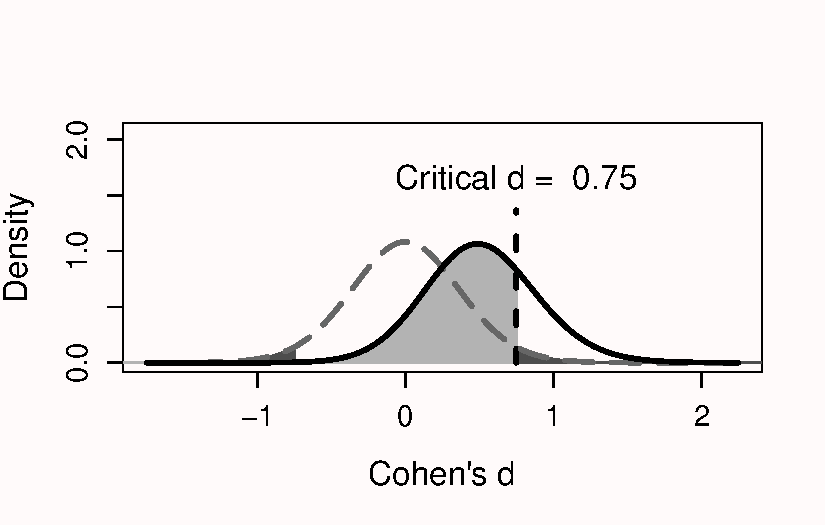
\includegraphics[width=1\textwidth,height=\textheight]{08-samplesizejustification_files/figure-pdf/fig-power-effect1-1.pdf}

}

\caption{\label{fig-power-effect1}独立样本 t 检验的临界效应量(每组 n =
15, \(lpha\)= 0.05 )}

\end{figure}

G*power在统计检验力分析时提供了的临界的统计量(如临界 t
值)。例如,图5显示,在\(\alpha\) = 0.05, N = 30
的双侧相关性检验中,只有效应大于 r = 0.361 或小于 r = -0.361
才能在统计学上显著。这表明,当样本量相对较小时,需要有相当的大效应才能达到统计学显著。

\begin{figure}

{\centering 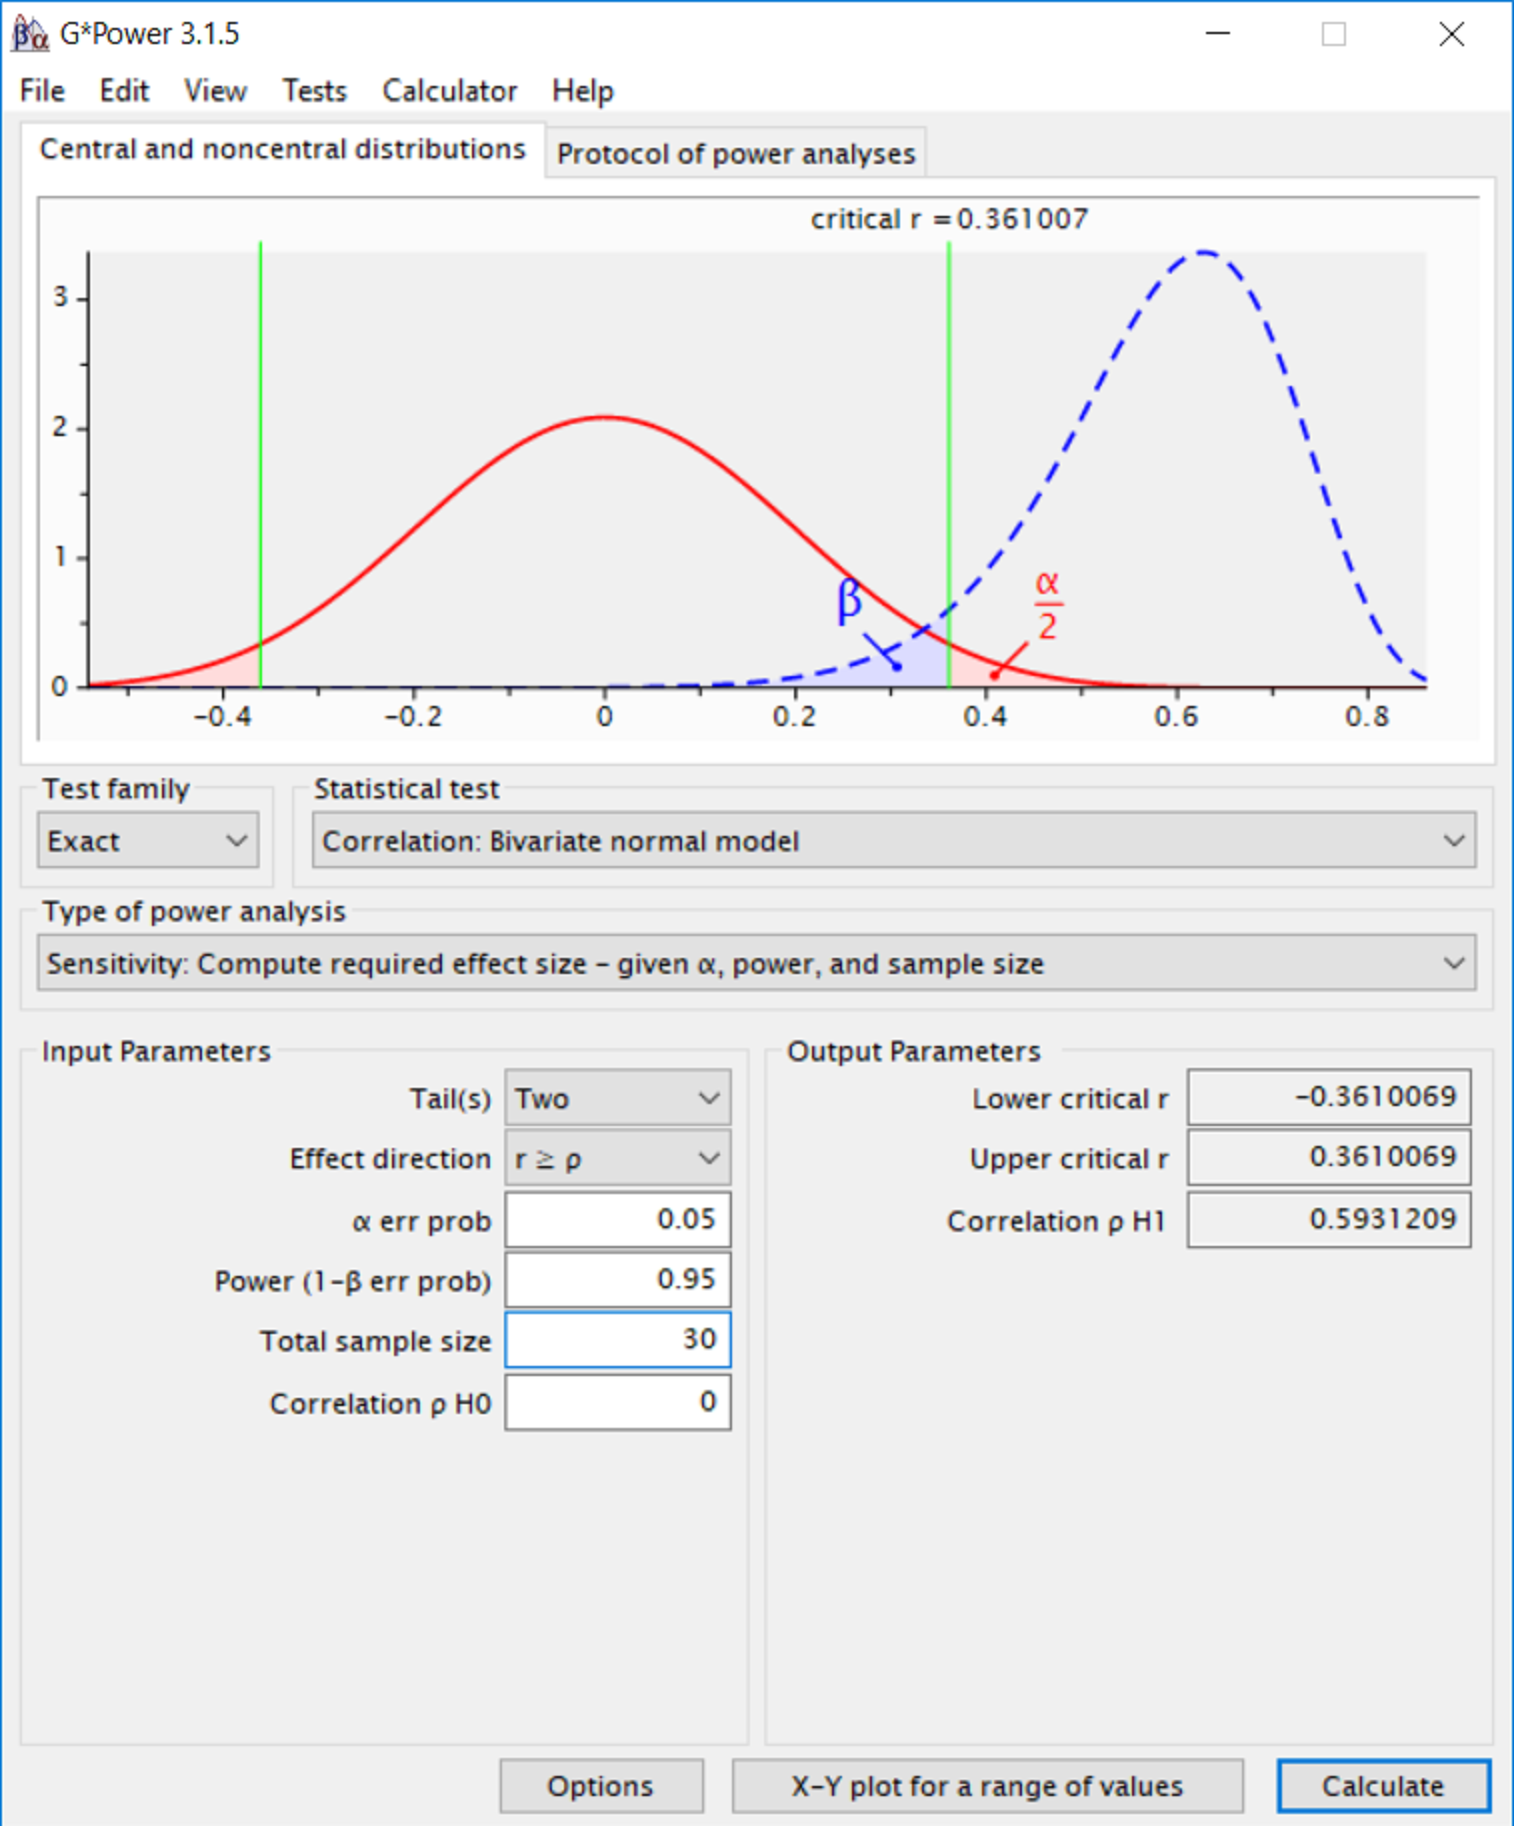
\includegraphics[width=1\textwidth,height=\textheight]{images/gpowcrit2.png}

}

\caption{\label{fig-gcrit2}G*power中相关性检验的临界值( n = 30 和
\(lpha\) = 0.05 )}

\end{figure}

重要的是要意识到,由于随机变异,每个研究都有概率产生大于临界效应量的效应,而真实的效应量很小
(当真正的效应量为0时,每个统计显著的效应都是一个 I
类错误)。计算统计显著的最小效应量(a minimal statistically detectable
effect)对于没有进行先验检验力分析的研究是有用的,这既适用于未报告样本量合理性的已发表研究
Lakens, Scheel, et al.
(2018),也适用于通过经验法则进行样本量论证的研究者。

扪心自问,你的研究设计的临界效应量是否在实际可预测的效应范围内?如果不是,那么当已发表的文章效应显著时,要么是效应量出乎意料地大于预期,或者更可能的是高估了效应量。后者,鉴于发表偏倚,已发表的文章可能会导致效应量估计走偏。如果仍有可能继续增加样本量,例如忽略以往经验并进行先验检验力分析,那么就继续。如果不继续增加样本量了,例如资源有限等,那么应该要明确最小统计显著效应,且此时不应该拘泥于
p 值,而是关注效应量以及其置信区间(如表 Table~\ref{tbl-table-pow-rec}
所述)。

如果进行了先验检验力分析,计算最小统计显著效应同样也有用。例如,如果您认为真实效应量的最佳情况是
d = 0.57
,并在先验检验力分析中采用了这个效应量,那么当您在一个包含两个独立组的研究设计中收集
50 个数据时,小于 d = 0.4
的效应量将不会在统计学上显著。如果备择假设的最坏情况是真实效应量为 d =
0.35
,那么当估计的效应量接近最坏情况时,您的研究设计将无法得到一个显著的结果。考虑到最小统计显著效应,你应该思考假设检验能否得到一个有意义的结果,以及你目前论证样本量合理性的方式(例如,使用经验法则,或者由资源支配来决定样本量大小)能否使研究更有意义。

\hypertarget{ux9884ux671fux7684ux6548ux5e94ux91cfux662fux4ec0ux4e48}{%
\section{预期的效应量是什么?}\label{ux9884ux671fux7684ux6548ux5e94ux91cfux662fux4ec0ux4e48}}

尽管效应量的真实分布往往是未知的,但在某些情况下,研究者将对其研究的效应量有一个合理的预期,并在先验检验力分析中使用这个预期效应量。即便从很大程度上来说,预期效应量是一种猜测,但斟酌哪些效应可以被预测是有用的。研究者可以根据他们预期的效应量来论证样本量的合理性,尽管从感兴趣的最小效应量的角度来看,这不会有很大的参考价值。因为在这种情况下,对推断目标是有价值的(检验预期效应是否存在),但对于次要目标(检验感兴趣的最小效应量是否存在)来说则没那么多的价值。

对于效应量分布的预测通常有三个来源:元分析、前人研究或理论模型。研究者倾向于在先验检验力分析时设置较高的预期效应量,因为较高的效应量需要的样本量较少,但对效应量的预期太过乐观将会增加结果假阴性的概率。在论证样本量(基于先验检验力分析)的合理性时,重要的是批判性地估量检验力分析中所使用的预期效应量。

\hypertarget{ux4f7fux7528ux6765ux81eaux5143ux5206ux6790ux4e2dux7684ux8bc4ux4f30}{%
\section{使用来自元分析中的评估}\label{ux4f7fux7528ux6765ux81eaux5143ux5206ux6790ux4e2dux7684ux8bc4ux4f30}}

通过元分析来估计效应量是最完美的,可以为研究者提供最准确的信息,来表明哪些效应是可预期的。由于学术领域普遍存在发表偏倚,来自元分析的效应量估计不一定是准确的。它们可能是有偏的,甚至有时是很大的偏差。此外,元分析通常具有相当大的异质性,这意味着元分析估计出的效应量与组成元分析的子集是不同的。因此,想要在检验力分析中使用元分析估计出的效应量,需要非常谨慎。

如果研究者想要在先验检验力分析中使用元分析估计出的效应量。他们需要考虑三个因素(见表
Table~\ref{tbl-tablemetajust}
)。首先,元分析中的研究和他们想要做的研究应该是比较相似的,这样才能够期望得到一个合理且相似效应量。本质上,这需要评估效应量的估计值在新研究中的可推广性。重要的是需要考量元分析中的研究和所计划的研究之间的差异,这涉及到实验操纵、测量、总体及其他相关变量。

其次,研究者应该检查与元分析所报告的效应量是否是同质的。如果不是,且异质性相当大,这意味着所估计出的效应量与真实值可能有所出入。使用元分析进行评估时,应采用最接近研究计划的研究子集。请注意,异质性仍有可能存在(当未测量的变量调节了样本的效应量时,即使是完全重复性的研究也可能表现出异质性(Kenny
\& Judd, 2019; Olsson-Collentine et al.,
2020),所以选择相似研究的主要目的是通过现有的数据来增加预估准确的概率,但不能保证它是绝对正确的。

最后,元分析的效应量估计应该尽可能没有偏差。核对元分析中报告的偏差检验测试(bias
detection test)是否是达到最高标准,或自己进行多次偏差检验测试(Carter et
al.,
2019),并采纳偏差校正后的效应量估计值(这些估计可能仍然存在偏差,并且不一定能反映真实的效应量分布)。

\hypertarget{tbl-tablemetajust}{}
\begin{table}
\caption{\label{tbl-tablemetajust}检验力分析中使用元分析来估计效应量时的建议 }\tabularnewline

\centering
\begin{tabular}{>{\raggedright\arraybackslash}p{5cm}|>{\raggedright\arraybackslash}p{10cm}}
\hline
需要参考的事项? & 需要怎么做?\\
\hline
与元分析中的研究是否相类似? & 元分析中的研究在实验设计,测量方法以及被试选取方面与你所计划的研究非常相似吗?评估效应量估计值在您研究中的可推广性。\\
\hline
与元分析中的研究是否同质? & 与元分析的研究是否存在异质性?如果是,请采用与你研究最相关的同质研究进行效应量估计。\\
\hline
效率量的估计是否无偏? & 原始研究是否报告了偏差检验测试(bias detection tests)偏差存在与否?如果存在,那么明智的做法可能是使用偏差校正手段来保守的估计效应量,并同时承认矫正后的估计效应量不等价于元分析的效应量估计。\\
\hline
\end{tabular}
\end{table}

\hypertarget{ux6839ux636eux524dux4ebaux7814ux7a76ux6765ux4f30ux8ba1ux6837ux672cux91cf}{%
\section{根据前人研究来估计样本量}\label{ux6839ux636eux524dux4ebaux7814ux7a76ux6765ux4f30ux8ba1ux6837ux672cux91cf}}

如果没有元分析研究作为参考,研究者通常会用某个前人研究的效应量来做先验检验力分析。首要需要考虑的问题是两个研究之间是否足够相似。与使用元分析估计效应量类似,研究者需要考虑不同研究在总体、实验设计、实验操纵、测量
以及其他可能影响效应量的因素上是否存在差异。例如,个体的反应时差异会随着年龄的增加而增加。因此,相比于年轻被试样本的研究,年长被试样本的研究标准效应量更小。其次,如果前人研究采用了一个强操纵,而你计划使用一个相对弱的实验操纵,那么将效应量预估地相对小一点会更适合。最后,效应量不能在不同实验设计的研究之间推广。例如,组间对比实验的效应量通常与后续实验中交互作用的效应量是不一样的,后者往往会在原实验设计的基础上添加新的变量,从而导致效应量的差异
(Lakens \& Caldwell, 2021)。

即便实验设计再相似,统计学家们也反对用预实验的效应量做检验力分析。Leon,
Davis 和Kraemer (2011) 认为:

\begin{quote}
与之相反,由于小样本固有的不精确性,预实验不能为后续的正式研究提供有意义的效应量估计值。
\end{quote}

利用已发表文章的效应量做检验力分析需要谨慎考虑,主要有以下两个原因:由于随机变异,前人研究中的效应量可能与真实的效应量分布不同;由于发表偏倚往往会夸大研究的效应量。图
Figure~\ref{fig-followupbias} 展示了某研究的分布,该研究一共 3
个条件,每个条件下 25
名被试,在零假设为真的情况下,存在''中等''的''真实''效应 (\(\eta_p^2\) =
0.0588) Richardson (2011)。图 Figure~\ref{fig-power-effect1}
标注了临界效应量,在小样本量下,观测到的效应量小于 \(\eta_p^2\) = 0.08
时在统计学上不显著。如果零假设为真,效应值大于 \(\eta_p^2\) = 0.08 会犯
I 类错误(深灰色区域)。如果备择假设为真,效应值小于 \(\eta_p^2\) = 0.08
会犯 II
类错误(浅灰色区域)。显然,显著结果的效应量都比真实效应量(\(\eta_p^2\)
= 0.0588 )要大
。因此,依据显著结果的效应量进行统计检验力分析(通常只有显著结果的研究能够被发表)
往往会高估真实效应量,从而产生偏差。

尽管测量了所有的效应量(e.g.,
从预实验中所得),由于随机差异,所得效应量有时还是会很小。如图
Figure~\ref{fig-followupbias} 所示,即使真实效应量只有 0.0588
,小样本的预实验所得效应量很可能有 \(\eta_p^2\) = 0.01
。将估计出的效应量 \(\eta_p^2\) = 0.01
用在先验检验力分析中,如果后续研究想要达到80\%的统计检验力,将会得出需要的总样本量为
957
。如果研究者仅根据预实验的效应量来计算(检验力分析)后续实验所需被试量,这样会高估效应量,从而导致后续实验的检验力系统性地低于我们的假设(Albers
\& Lakens, 2018)。

\begin{figure}

{\centering 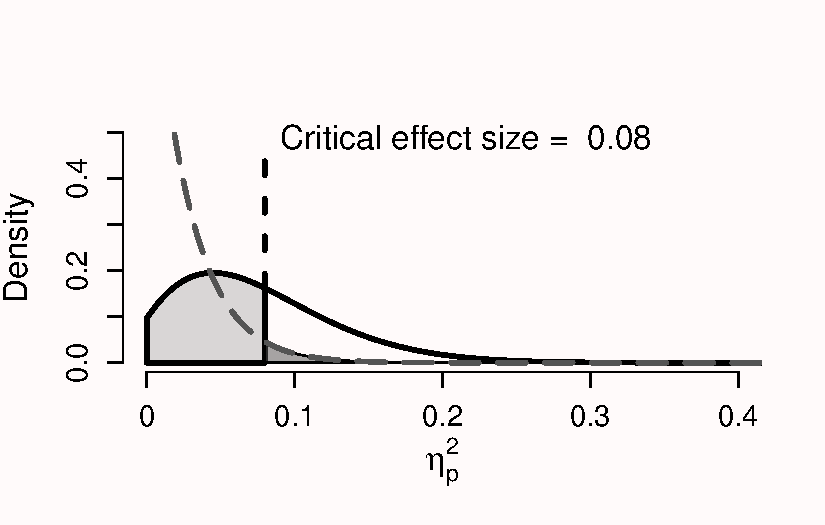
\includegraphics[width=1\textwidth,height=\textheight]{08-samplesizejustification_files/figure-pdf/fig-followupbias-1.pdf}

}

\caption{\label{fig-followupbias}零假设为真(虚线灰色曲线)以及真实效应量中等大小(\(\eta_p^2\)
= 0.0588 ,实线黑色曲线)情况下的 分布(3 组,各 25 名被试)。}

\end{figure}

归根结底,通过小样本研究来估计效应量(用于先验检验力分析)存在本质上的问题,由于发表偏倚或后续的偏差,也就是说研究者最终用于检验力分析的效应量并不是基于完整的F分布,而是基于截断的
F(truncated) 分布(Taylor \& Muller, 1996)。例如,假设图
Figure~\ref{fig-followupbias}
所展示的是一个极端的发表偏倚情况。研究者只能得到图中 \(\eta_p^2\)
\textgreater{} 0.08
的部分分布,这些结果均在统计学上达到显著。这种情况下,也能够求得基于特定假设且经过偏差矫正后的效应量(估计的)。假设,单因素3水平的研究的方差分析结果是
F(2, 42) = 0.017 , \(\eta_p^2\) = 0.176
。如果我们在先验检验力分析中使用这个效应量,那么为了得到 80\%
的统计检验力,每个条件需要的样本量为 17 名被试。

然而,偏差已然存在,我们可以用BUCSS R包(S. F. Anderson et al., 2017)
进行检验力分析来尝试校正偏差。校正偏差后的检验力分析结果显示(基于特定发表偏倚模型的截断F分布,即只有显著结果能被发表),每个条件下需要的样本量为73名被试。当用于计算检验力的非中心参数的偏差校正估计值为零时,此方法则不再适合。相对的,只要研究者认为存在偏差,就可以做一个偏差校正模型。一个相对简单且更保守的方式是,用效应量估计出
60\% 双侧置信区间的下限来进行检验力分析。此法被 Perugini et al. (2014)
称为''保底检验力''(safeguard
power)。上述提到的两种方式都是相对保守的检验力分析,但并不能一定是更准确的估计。因为基于一个可能存在偏差的且/或样本量较小的研究效应量,几乎不可能完成一个准确的检验力分析(Teare
et al.,
2014)。在无法得到感兴趣的最小效应量时,对效应量的估计存在极大的不确定性。这种情况下用序列设计(sequential
design)来进行实验相对更高效。

总而言之,如果满足以下三个条件(表
Table~\ref{tbl-table-es-just}),则可以利用前人研究的效应量做检验力分析。第一,研究设计与前人研究足够相似。第二,偏差存在的风险较低。(例如,效应量的估计是源于预注册的报告,或者是没有影响发表可能性的实验结果报告,即无关发表偏倚)。第三,基于95\%置信区间的所得效应量,样本量足够大,可以得到相对准确的效应量估计。效应量估计总是伴随着不确定性,因此进行先验检验力分析时,将95\%置信区间的上下限都考虑进来,可能会为这些不确定性提供一些有效的信息。

\hypertarget{tbl-table-es-just}{}
\begin{table}
\caption{\label{tbl-table-es-just}检验力分析中使用单项研究来估计效应量时的建议 }\tabularnewline

\centering
\begin{tabular}{>{\raggedright\arraybackslash}p{5cm}|>{\raggedright\arraybackslash}p{10cm}}
\hline
需要参考的事项? & 需要怎么做?\\
\hline
研究是否足够相似? & 考虑研究之间在总体、实验设计、实验操纵、测量方法或其它方面的差异,从而导致期望效应有所不同。\\
\hline
是否存在偏差的风险? & 如果效应量估计值较小,评估您不会采用(或不会发表)它的可能性。在统计检验力分析时,比较校正偏差前后的估计效应量的差异。\\
\hline
不确定性有多大? & 被试量较少的研究具有更大的不确定性。考虑使用更加保守的效应量估计的可能性,以降低真实效应量的统计检验力不足的可能。\\
\hline
\end{tabular}
\end{table}

\hypertarget{ux6839ux636eux7406ux8bbaux6a21ux578bux6765ux4f30ux8ba1ux6837ux672c}{%
\section{根据理论模型来估计样本}\label{ux6839ux636eux7406ux8bbaux6a21ux578bux6765ux4f30ux8ba1ux6837ux672c}}

你可以根据一个足够详细、具体的理论模型来搭建一个计算模型,并根据这个计算模型来估计效应量,前提是你十分了解模型中与数据收集相关的核心参数有哪些。例如,如果研究者对每个刺激特征之间的异同的权重十分了解,那么可以通过(Tversky,
1977) 的对比模型计算每对刺激的相似性判断预测(predicted similarity
judgement),以及估计不同条件之间差异的预期效应量。尽管可以做点估计的计算模型相对稀少,但合适的模型常常可以为研究者的预期效应量提供强有力的证据。

\hypertarget{ux8ba1ux7b97ux6548ux5e94ux91cfux7684ux7f6eux4fe1ux533aux95f4ux5bbdux5ea6}{%
\section{计算效应量的置信区间宽度}\label{ux8ba1ux7b97ux6548ux5e94ux91cfux7684ux7f6eux4fe1ux533aux95f4ux5bbdux5ea6}}

如果研究者能够估计数据的标准差,那么就有可能预先估计出效应量的 95\%
置信区间(Kelley,
2007)。置信区间表示的是一个估计值的范围,这个范围足够宽,真正的总体参数将会落在置信区间
(100-\(\alpha\))\%
的范围内。在任何单项研究中,真正的总体效应要么落在置信区间内,要么不在置信区间内,但总地来说,人们可以认为置信区间包括了真实的总体效应(要记得存在犯错的可能)。Cumming
(2013) 将得到的效应量与 95\% 置信区间上限(或 95\%
置信区间下限)之间的差距称为误差幅度(margin of error)。

如果我们根据 t 值和样本量计算效应量为 d = 0 的 95\% 置信区间(Smithson,
2003),就会发现,当独立样本 t 检验的每个条件下各有 15 个观测值时, 95\%
置信区间的范围从 d = -0.716 到d =
0.716。效应量的置信区间可以使用在线应用程序来计算:https://www.aggieerin.com/shiny-server/。
误差幅度是 95\% 置信区间宽度的一半,即 0.716
。使用无先验信息的贝叶斯估计将计算出一个具有相同(或非常相似)上限和下限的置信区间(Albers
et al., 2018; Kruschke,
2011),并且在收集完数据后,可能得出一个包含总体效应的范围,但范围太大并不能提供信息。不论在分析数据时基于哪种统计学派,在每组只有
15 个观测值的情况下所得的置信区间范围,并不能使我们获得更多信息。

对置信区间宽度的有效解释之一是,当真实效应量为 0
时,效应量多大时你可以拒绝该效应。换句话说,如果效应不存在,根据收集到的数据情况,你能够拒绝哪些效应量?哪些效应量不会被拒绝?以下这些研究有
d = 0.7
的效应量,比如''人们在被激怒时变得具有攻击性'',``相比于其他群体,人们更喜欢自己的群体'',以及''恋爱对象在外表吸引力上彼此相似''(Richard
et al.,
2003)。根据置信区间的宽度,只能拒绝过大的效应,如果效应真实存在,那么应该已经被发现了。如果你研究的大多数效应比
d = 0.7 小得多,那么通过 n = 15
的研究,很可能发现不了任何东西。在大多数研究领域,过大的效应通常被认为是不合理的(尽管合理的效应量大小在不同领域之间是不同的,如下所述)。然而,例如在大样本中,如果零假设是真的,研究者可以拒绝大于
d = 0.2
的效应。而根据置信区间宽度的分析,许多研究领域的同行可能会认为这项研究是有价值的。

我们发现,误差幅度几乎与统计上可检测到的最小效应( d =
0.748)相同,但并不完全相同。这个小的变异来源于根据 t 分布计算的 95\%
置信区间。如果真正的效应量不为零,则根据非中心 t
分布计算置信区间,那么得到的 95\% 置信区间是不对称的。图
Figure~\ref{fig-noncentralt} 显示了三个 t 分布,一个在 0
处对称分布,另外两个分别在 2 和 3
的非中心参数(均值之间的标准化差异)的不对称分布。这种不对称性在非常小的样本中最为明显(图中的分布自由度为
5
),但在计算置信区间和统计检验力时,在较大的样本中也很明显。例如,当真实效应量为
d = 0.5 时,每组15个观测值的效应量为 = 0.50 , 95\% 置信区间为 {[}-0.23,
1.22{]}。如果我们计算临界效应量的 95 \%置信区间,将得到 = 0.75 , 95\%
置信区间为 {[}0.00, 1.48{]} 。95\%置信区间的范围从 0.00 到 1.48
,这与置信区间和 p
值之间的关系一致,也就是说如果检验有统计学意义(结果显著),那么 95\%
的置信区间不包括 0
。正如前面提到的,这里推荐的不同方法,通常是基于相同的信息来评估研究价值。

\begin{figure}

{\centering 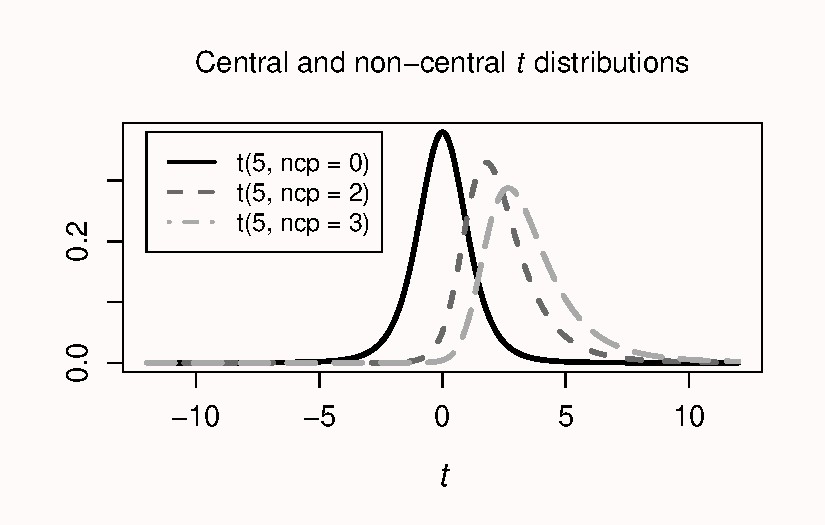
\includegraphics[width=1\textwidth,height=\textheight]{08-samplesizejustification_files/figure-pdf/fig-noncentralt-1.pdf}

}

\caption{\label{fig-noncentralt}中心的(黑色)和2个非中心的(深灰和亮灰)
t 分布}

\end{figure}

\hypertarget{ux7ed8ux5236ux7075ux654fux5ea6ux529fux6548ux5206ux6790ux56fe}{%
\section{绘制灵敏度功效分析图}\label{ux7ed8ux5236ux7075ux654fux5ea6ux529fux6548ux5206ux6790ux56fe}}

灵敏度功效分析确定了样本量、期望检验力和\(\alpha\)水平,并回答了在期望检验力下研究能获得多少效应量的问题。因此,当样本量已知时,就可以进行灵敏度分析。有时,我们使用的是已经回答过不同研究问题的现成数据,或者从现有数据库中抽取的一部分,此时样本量已知,你可以为新的统计分析进行灵敏度功效分析。而其他时候,你可能在最初收集数据时没有仔细考虑样本量的问题,但希望在分析结果时反映出该研究对感兴趣的效应量(范围)的统计检验力。最后,虽然有可能在未来会收集到足够的样本量,但是由于资源限制,你知道你能够收集的最大样本量是有限的。你希望对于你认为合理且有趣的效应(例如感兴趣的最小效应大小或预期的效应大小)是否具有足够的统计检验力进行反思。

假设某研究者正进行一项研究,总共将收集 30 个样本,每个条件下各 15
名被试。图 Figure~\ref{fig-gsens0}
显示了如何在G*power中进行灵敏度功效分析,在该研究中,我们决定使用 5\% 的
\(\alpha\) 水平,并希望获得 90\%
的检验力。灵敏度功效分析结果显示,研究设计有 90\% 的检验力来检测 d =
1.23
以上的效应。有研究者认为90\%的期望检验力是相当高的,并且认为如果统计检验力更低的话,仍然可以开展一项有趣的研究。因此,在小效应量范围内绘制灵敏度曲线是很有用的。

\begin{figure}

{\centering 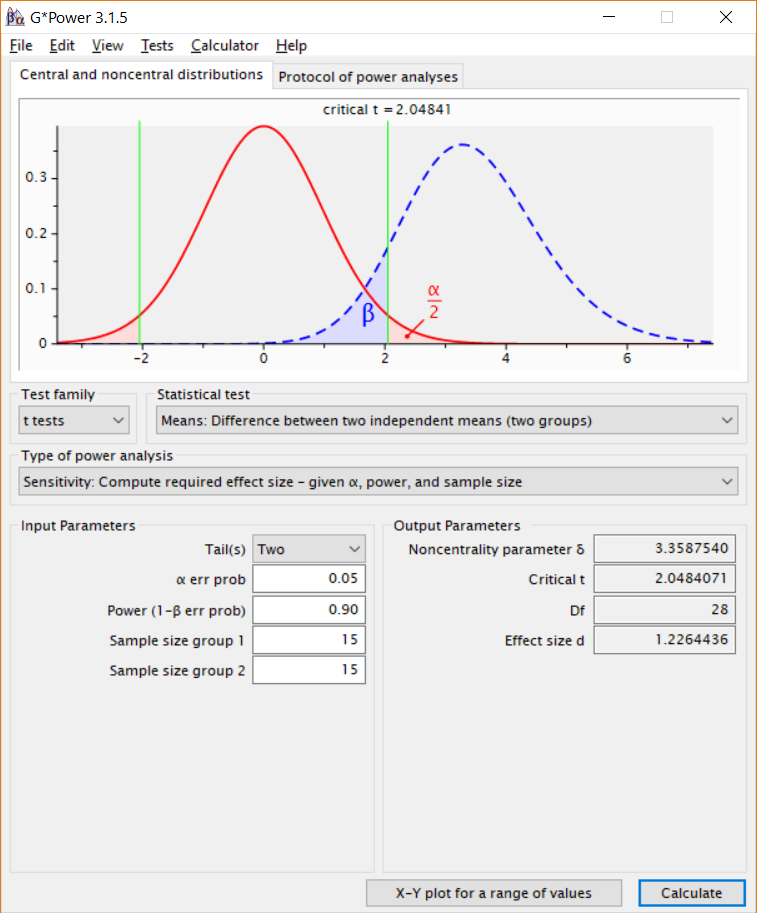
\includegraphics[width=1\textwidth,height=\textheight]{images/gpow_sensitivity_1.png}

}

\caption{\label{fig-gsens0}G*Power软件中的灵敏度功效分析}

\end{figure}

在灵敏度检验力分析中,有重要的两个维度:效应量以及检验力(即特定的效应量显著时的检验力)。这两个维度可以共同绘制灵敏度曲线。例如,在G*Power中,可以通过点击''X-Y
plot for a range of values''按钮来绘制灵敏度曲线,如图
Figure~\ref{fig-gsens1}
所示。研究者可以检测合理的先验效应量范围的检验力,或者他们可以检测哪些效应量将提供合理的检验力水平。在基于模拟的检验力分析方法中,可以通过对一系列可能的效应量进行检验力分析来创建灵敏度曲线。即使50\%的检验力被认为是可以接受的(此时如若得到不显著的结果之后,是否接受零假设,是一个相对复杂的决策过程),图
Figure~\ref{fig-gsens1}
显示了一个检验力非常低的研究,这对于大多数领域来说是属于较大合理范围内的效应量。因此,灵敏度功效分析为评估研究价值提供了额外的方法,并可以提示研究者,对于在某些特定的实验设计下,一些实际预期范围内的效应不太可能产生显著的结果。

\begin{figure}

{\centering 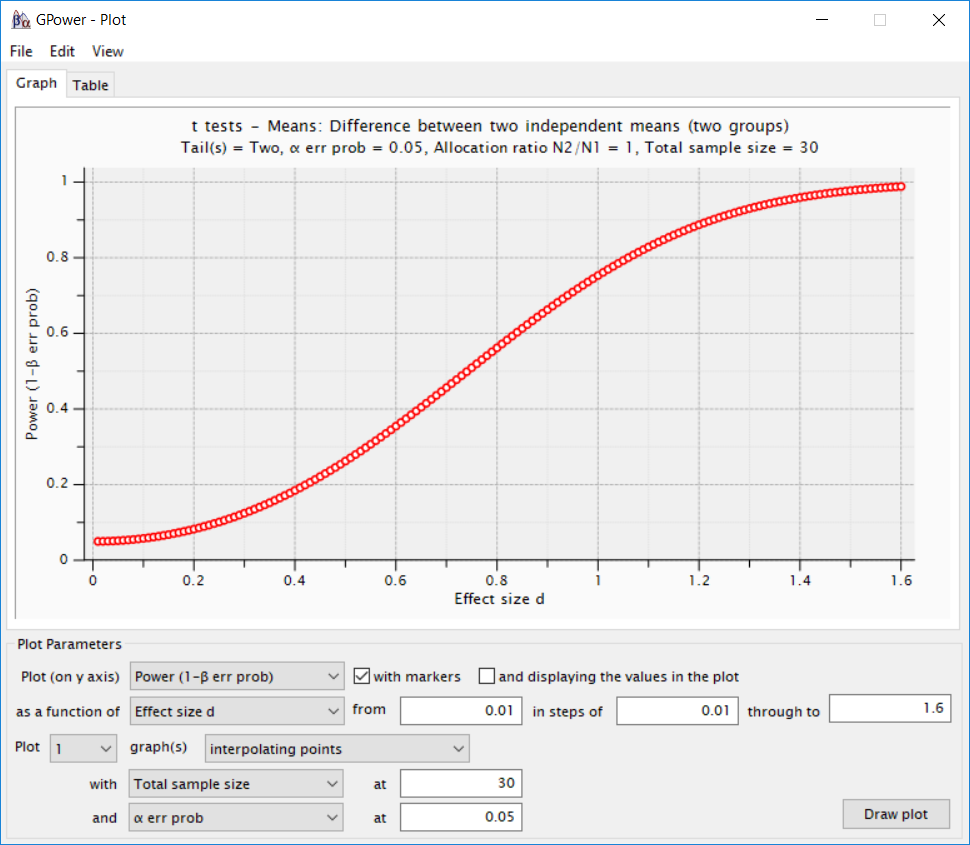
\includegraphics[width=1\textwidth,height=\textheight]{images/sensitivity1.png}

}

\caption{\label{fig-gsens1}当每组 n = 15, \(\alpha\) = 0.05
时,效应量与期望检验力的关系图}

\end{figure}

如果每组的被试量更大,评估结果可能会更好。虽然我们不知道效应量究竟多大,但如果每组收集150个被试,灵敏度分析结果显示感兴趣效应的检验力是足够的,此外,对于相当小的效应,仍有大约为50\%的检验力。为了使灵敏度分析有意义,灵敏度曲线应该与感兴趣的最小效应量或预期的效应量范围进行比较。灵敏度功效分析没有明确的界限可供参考(Bacchetti,
2010)。但我们可以在人们观测到的或关心的不同效应量及其相关的统计检验力之间进行总体权衡。

\hypertarget{ux6548ux5e94ux91cfux5728ux7814ux7a76ux9886ux57dfux7684ux5206ux5e03}{%
\section{效应量在研究领域的分布}\label{ux6548ux5e94ux91cfux5728ux7814ux7a76ux9886ux57dfux7684ux5206ux5e03}}

根据我个人的经验,在独立样本 t
检验的先验检验力分析中,最常输入效应量估计是Cohen's基准的''中等''效应量,这是默认的一个效应量。当你打开
G*Power
时,``中等''效应是先验检验力分析的默认选项。其实,Cohen's基准的小、中、大效应不应该用于先验检验力分析
(J. Cook et al., 2014; Correll et al.,
2020),而且Cohen本人后悔提出了这些基准(Funder \& Ozer,
2019)。研究主题的多样性意味着,任何用于计算统计检验力的''默认的''或''经验法则式方法的''不仅不符合你的实际情况,还可能导致样本量与你试图用数据来回答的研究问题之间有很大的差距。

研究者想知道,如果没有其他依据来确定先验检验力分析的效应量,那么如何选默认值更好呢?Brysbaert
(2019) 建议心理学领域可以将 d = 0.4
作为默认值,这是在可重复的项目和若干元分析中观测到的平均水平。我们无法知道这个平均效应量是否可行,但很明显,各个领域和研究问题之间存在着巨大的异质性。平均效应量通常都与研究中预期的效应量有很大偏差。一些研究者建议根据效应量在特定领域的分布来更新Cohen's
基准(Bosco et al., 2015; Funder \& Ozer, 2019; Hill et al., 2008; Kraft,
2020; Lovakov \& Agadullina,
2021)。当我们基于已发表的文章来估计效应量时,需要考量效应量由于发表偏倚而被夸大的可能性。由于某一特定研究领域内的效应量存在较大的差异,所以基于某一领域内效应量的经验分布,选择一个大、中、小的效应量基准来进行检验力分析的用处不大。

在解释效应量的置信区间时,应该了解一些文献中效应量的分布。如果在一个特定的研究领域里,几乎没有效应大于你在等价检验中可以拒绝的效应量(例:如果观测到的效应量为
0 ,设计将只拒绝大于如 d = 0.7
的效应),那么,此时收集到的数据不太可能获得有用的信息。

我们很难找到依据来证明的是:从效应量的经验分布中推导出的特定效应量,可以作为先验检验力分析中使用的效应量。有人可能会说,使用文献中效应量分布的效应量基准比胡乱猜测要好,但这并不是论证样本量合理性的强证据。研究者们必须承认,在预期效应量不明确的情况下,不能进行先验检验力分析(Scheel,
Tiokhin, et al.,
2021)。而其他论证样本合理性的理由,比如资源限制,或者结合序列研究设计(a
sequential study design),可能可以更好地来满足研究的推断目标。

\hypertarget{ux8bbeux8ba1ux5b9aux6027ux7814ux7a76informative-studyux65f6ux7684ux6ce8ux610fux4e8bux9879}{%
\section{设计定性研究(informative
study)时的注意事项}\label{ux8bbeux8ba1ux5b9aux6027ux7814ux7a76informative-studyux65f6ux7684ux6ce8ux610fux4e8bux9879}}

到目前为止,我们一直把重点放在定量研究的样本量论证。其中有许多相关的主题对设计定性研究也有一定的帮助。首先,除了先验检验力分析以及灵敏度功效分析之外,探讨折中检验力分析(compromise
power analysis)(有帮助的)和事后检验力分析(没有帮助的,例如,Zumbo \&
Hubley (1998), Lenth
(2007))同样十分重要。如果能够通过先验检验力分析来确定样本量,那么序列设计的数据收集会非常有效,因为我们随时对收集到的数据进行分析来决定是否继续实验。此外,在不增加样本量的前提下提高研究统计检验力的方法非常有价值。另外,研究者应当充分了解自己实验的因变量,尤其是因变量的标准差。最后,样本量的规划在定性研究中同样重要,尽管在定性研究的领域内有关样本量规划的研究较少,但我们给出了一些建议,可供研究者们设计定性研究时参考。接下来我们将依次讨论上述每一点。

\hypertarget{ux6298ux4e2dux68c0ux9a8cux529bux5206ux6790compromise-power-analysis}{%
\section{折中检验力分析(compromise power
analysis)}\label{ux6298ux4e2dux68c0ux9a8cux529bux5206ux6790compromise-power-analysis}}

在折中检验力分析中,样本量和效应量是固定的,且检验的错误率是依据I类错误和II类错误之间的期望比(相对重要程度之比,desired
ratio)所计算出来的。当需要收集大量的数据或者只能收集少量数据时,折中检验力分析都是有用的。

前者,因为研究者们十分幸运地能够收集到足够多的数据,所以对于研究者们所有感兴趣的效应量而言,研究的统计检验力都很高。比如,研究者想在某一公司测试一种能够降低压力水平的干预措施,因此招募2000名雇员在公司的年度评估中回答了一系列问题。小于
d = 0.2 的效应不足以引起个体的主观注意(Jaeschke et al., 1989)。当
\(\alpha\) 水平为 0.05 时,统计检验力为 0.994,即犯 II 类错误的概率为
0.006。这意味着当感兴趣的最小效应量为d = 0.2时,研究者犯 I
类错误的可能性是犯 II 类错误可能性的 8.3 倍。

尽管研究者最初提出控制 I 类错误和 II
类错误,是为了论证其错误率合理性(Neyman \& Pearson,
1933),但一个常见的错误想法是:将 I 类错误设定为 0.05 ,II类错误为 0.2
,意味着 II 类错误发生的概率是 I 类错误的 4
倍。通常,默认使用80\%的检验力(或者 20\% 的 II 类错误)是基于 Cohen
(1988) 个人的偏好,他对此解释道:

\begin{quote}
这是一个惯例,当研究者没有其他依据来设置所需的检验力值时,默认采用 0.80
。这意味着 \(\beta\) ( II 类错误)被设定为 0.20
。采取这个值有以下几个原因(Cohen, 1965,第98-99页)。首先,主要考虑到
\(\alpha\) = 0.05 这个隐含条件。其次,选取 0.20
的\(\beta\)值是考虑到这两种误差的相对严重性之比为 0.20/0.05
。即第一类错误的严重程度是第二类错误的四倍。之所以提出 0.80
的检验力值是因为当研究者找不到依据来确定检验力时可以参考,但当研究者在其具体的研究调查中找到实质性的依据来选择一个特定值时,可以不采用这个值(This
.80 desired power convention is offered with the hope that it will be
ignored whenever an investigator can find a basis in his substantive
concerns in his specific research investigation to choose a value ad
hoc.)。
\end{quote}

我们可以看到,约定是基于其他约定之上的:即, 80\% 检验力的标准是基于
\(\alpha\) 水平为 0.05 的标准之上的。因此,我们从Cohen那学到的不应是以
80\%
的检验力为目标,而是应当基于每个错误的相对严重性,来论证错误率的合理性。这就是折中检验力分析的用处。如果你和Cohen有一样的信念(即
I 类错误的严重程度是 II
类错误的四倍),那么回到之前所提出的2000名雇员的研究,对所有感兴趣的效应量而言,当
II 类错误率较低时,调整 I 类错误率是有意义的(Cascio \& Zedeck,
1983)。实际上,Erdfelder et al. (1996)
开发G*Power软件,在一定程度上为研究者们提供了一个做折中检验力分析的工具。

\begin{figure}

{\centering 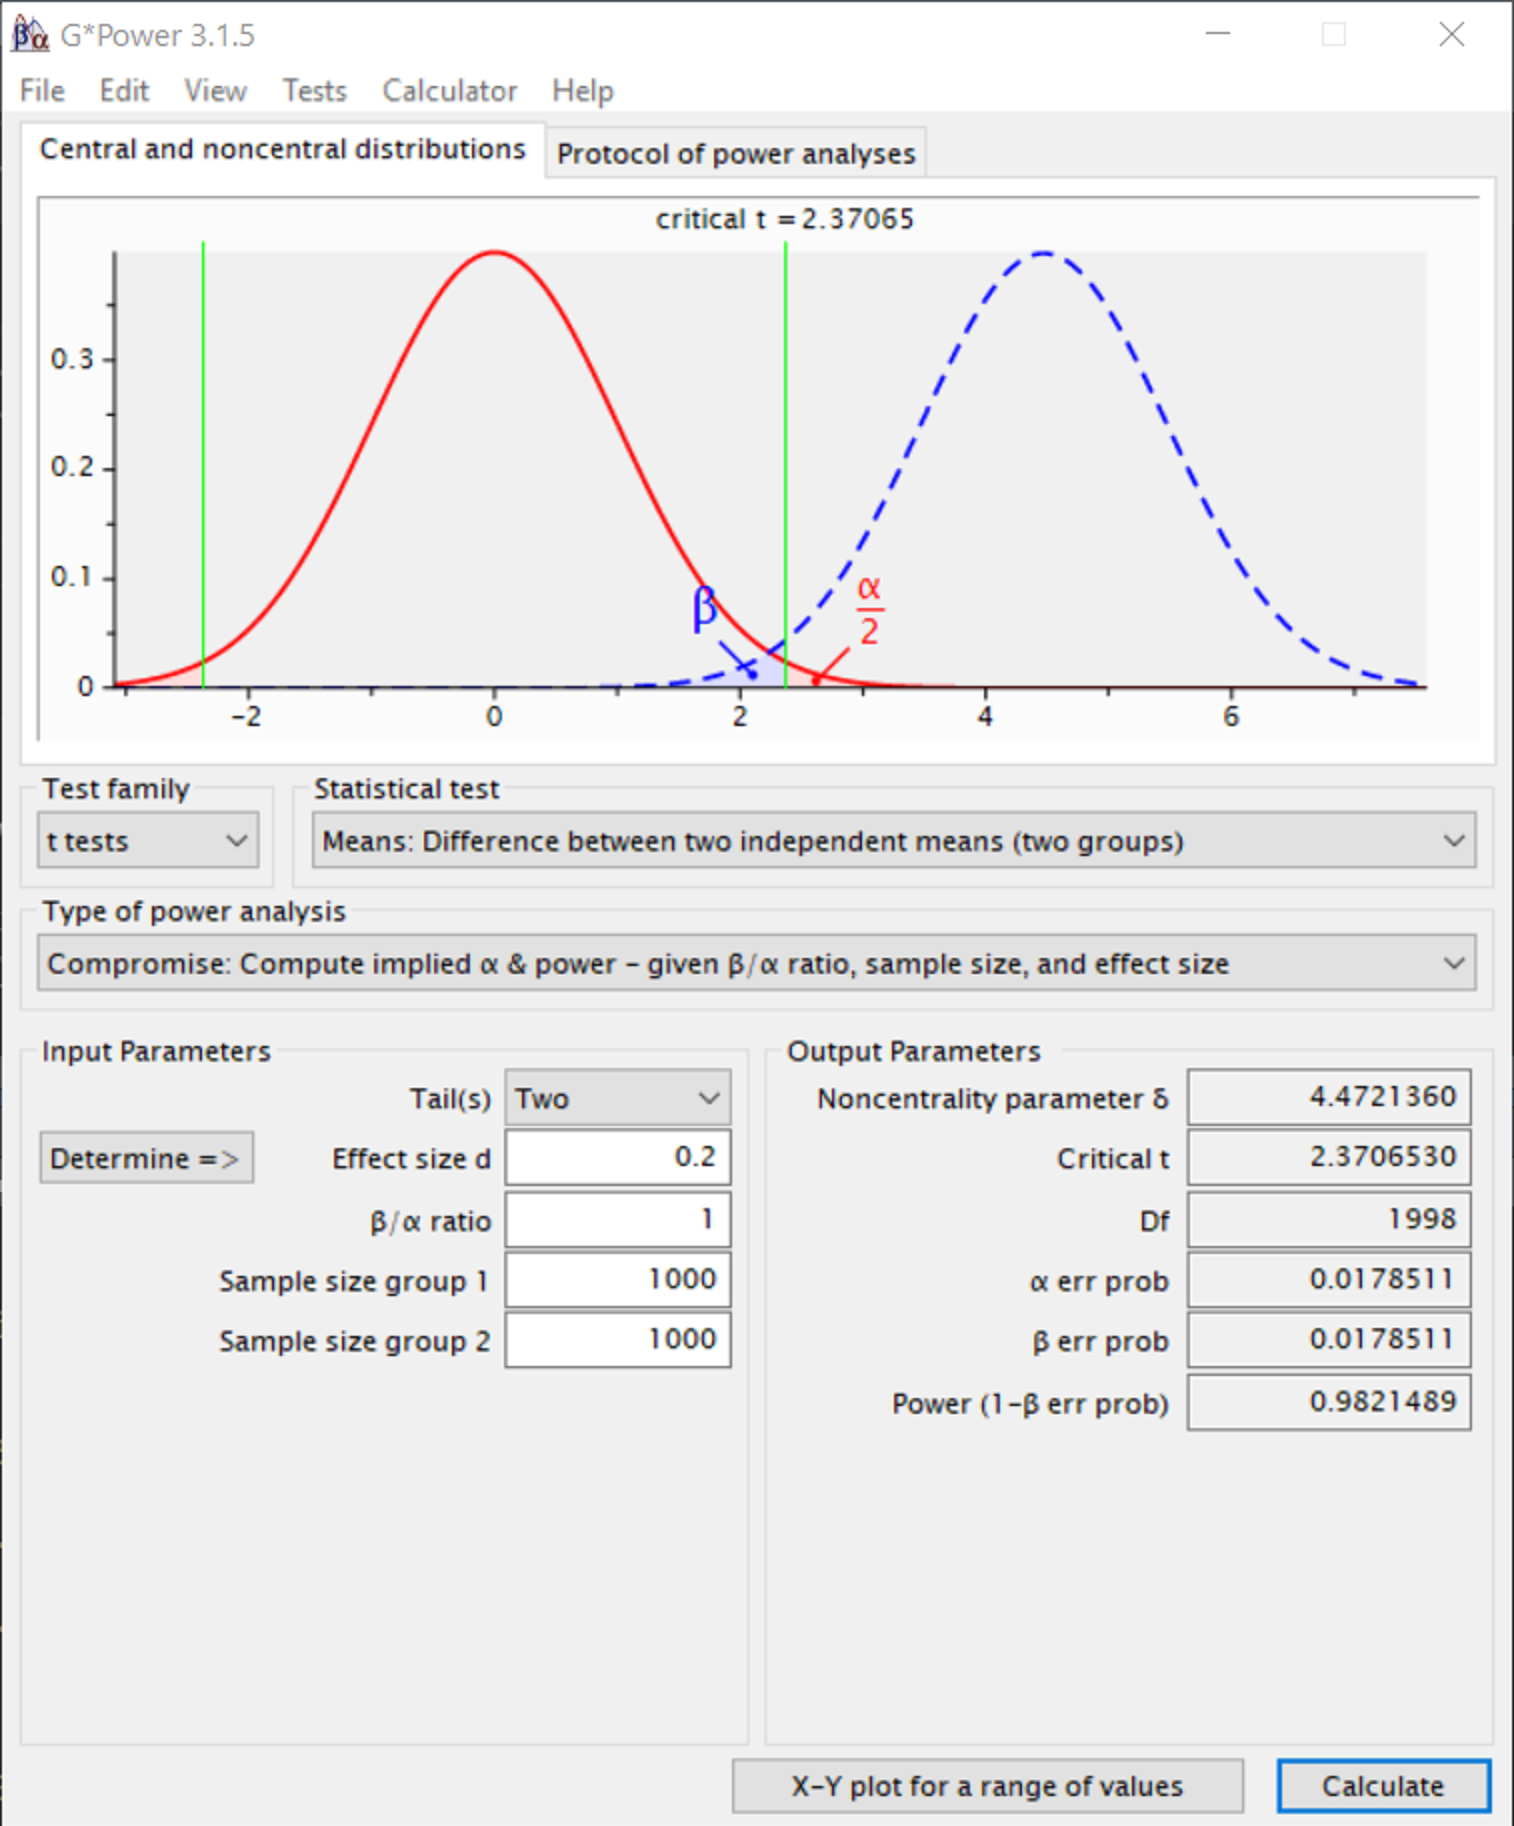
\includegraphics[width=1\textwidth,height=\textheight]{images/compromise1.png}

}

\caption{\label{fig-gpowcompromise}G*power中的折中检验力分析}

\end{figure}

Figure~\ref{fig-gpowcompromise} 展示了当I类错误的代价等同于 II
类错误时( \(\beta\)/\(\alpha\) ratio为 1
时),在G*Power中做折中检验力分析的情况,当每个条件有 1000 个被试时, I
类错误和 II 类错误均为 0.0179 。正如Faul,Erdfelder,Lang以及Buchner
(2007) 所描述的:

\begin{quote}
显然,折中检验力分析很容易导致非常规的显著性水平,也就是大于 \(\alpha\)
= 0.05 (在小样本或小效应量的情况下)或小于 \(\alpha\) = 0.001
(在大样本或者大效应量的情况下)。然而我们相信,平衡 I 类错误和 II
类错误风险的益处能够弥补违反显著性水平约定( \(\alpha\) = 0.05
)的代价。
\end{quote}

这将指引我们了解折中检验力分析发挥其他作用的情况,即当我们知道研究的统计检验力很低时。虽然在错误率很高时做决定是非常不可取的,但当研究者发现自己必须基于较少的信息作出决策时,Winer
(1962) 认为:

\begin{quote}
经常使用 0.05 或 0.01
作为显著性水平是一种约定俗成的惯例,但基本上没有科学性和逻辑性可言。在上述显著性水平下,如果研究的检验力很低,并且当
I 类错误和 II 类错误的重要性大致相同时, 0.30 和 0.20 的显著性水平可能比
0.05 和 0.01 的显著性水平更为合适。
\end{quote}

例如,我们计划做一个双侧 t 检验,每个独立组最多能够收集 50
个样本,且预期总体效应量为0.5,如果将 \(\alpha\) 水平设置为 0.05
,检验力将会达到 70\%
。同样,我们可以平衡两类错误(使其重要性相等),并将 \(\alpha\)
水平设置为 0.149 ,最终得到效应量为 d = 0.5 且统计检验力为 0.851
(即给定一个 0.149 的 II 类错误率)。在折中检验力分析下 \(\alpha\) 和
\(\beta\) 的选择,可以扩展到虚无假设和备择假设先验概率的考量当中(Maier
\& Lakens, 2022; Miller \& Ulrich, 2019; Murphy et al., 2014)。

折中检验力分析需要研究者确定样本量的大小。这个样本量的大小就需要进行合理性论证,因此折中检验力分析通常与资源受限的样本量一起进行权衡。如果你的资源有限,又迫切的需要做出决策,那么折中检验力分析非常关键。在这种情况下,研究者应该认真考虑一个可接受的
I 类和 II
类错误率。然而,当一个研究的样本量很大,但研究者仍不能自由设置样本量时,折中检验力分析仍然是有意义的。例如,收集的是一项较大的国际研究中的一部分数据,且样本量是基于其他研究问题得来。在II类错误率非常低(且检验力很高)的研究设计中,一些统计学者认为还应当降低α水平来防止林德利悖论(Lindley's
paradox),在林德利悖论中,效应显著( p \textless{} α
)是对零假设的某种证明(Good, 1992; Jeffreys,
1939)。降低统计检验力分析中的α水平可以防止该悖论的产生,这就为大样本量的折中检验力分析提供了另一种依据(Maier
\& Lakens,
2022)。最后,折中检验力分析需要对效应量进行合理论证,要么基于感兴趣的最小效应量,要么基于预期的效应量。表
Table~\ref{tbl-table-compromise-just}
列出了应该与折中检验力分析一起讨论的三个方面。

\hypertarget{tbl-table-compromise-just}{}
\begin{table}
\caption{\label{tbl-table-compromise-just}依据折中检验力分析来权衡错误率合理性时的一些建议 }\tabularnewline

\centering
\begin{tabular}{>{\raggedright\arraybackslash}p{5cm}|>{\raggedright\arraybackslash}p{10cm}}
\hline
需要参考的事项 & 该怎么做?\\
\hline
样本量的合理论证 & 说明为什么要收集特定的样本量(例如,基于资源的限制或决定样本量的其他因素)。\\
\hline
效应量的合理论证 & 效应量的大小是基于感兴趣的最小效应量,还是所预期的效应量。\\
\hline
I 类错误和 II 类错误之间的期望比(相对重要程度之比,desired ratio) & 通过仔细评估每类错误的后果来权衡二者的相对代价。\\
\hline
\end{tabular}
\end{table}

\hypertarget{sec-posthocpower}{%
\section{如果期刊编辑要求事后统计检验力,该怎么办?}\label{sec-posthocpower}}

事后检验力、回溯性检验力或观察性检验力被用于描述效应量(假设从收集到的数据估算出的效应量是真实的效应量)的统计检验力(Lenth,
2007; Zumbo \& Hubley,
1998)。所以,在收集数据之前,无法计算事后检验力,它并不像先验检验力分析那样,可以基于感兴趣的效应量来进行估计,而且它也不像灵敏度功效分析那样,可以对一系列感兴趣的效应量进行估计。因为事后检验力是基于已收集数据的效应量,除了报告的
p
值之外,没有增添其他信息,但它以不同的方式呈现了相同的信息。编辑和审稿人经常要求作者用事后检验力分析来解释不显著的结果。这不是一个合理的要求,无论何时提出,你都不应该遵从。相反,你应该进行灵敏度功效分析,并讨论感兴趣的最小效应量的检验力,以及预期效应量的一个实际范围。

事后检验力与统计检验中的 p 值直接相关(Hoenig \& Heisey, 2001)。对于 p
值恰好为 0.05 的 z 检验,事后检验力始终为 50\%
。产生这种关系的原因是,当所得 p 值等于 α
水平(例如0.05)时,所得z分数正好等于检验显著的临界值(例如,在一个 α
水平为 5\% 的双侧检验中, z = 1.96
)。当备择假设以临界值为中心时,如果备择假设为真,我们预期所得数据的一半数据会低于临界值,而另一半数据会高于临界值。所以,在事后统计检验力分析中,如果假定分析的效应量为真,那么
p 值与 α 水平相同的检验,其统计检验力恰好为 50\% 。

对于其他统计检验来说,当备择假设的分布不对称时(例如 t
检验,备择假设遵循非中心化的 t 分布,如图 Figure~\ref{fig-noncentralt}
所示),一个 p = 0.05 时检验力不为 50\%
,但是通过对p值和检验力绘图,我们发现这两个统计量总是直接相关的。如图
Figure~\ref{fig-obs-power-plot-2} 所示,如果 p
值显示不显著(即,大于0.05时),那么可得知在 t 检验中检验力将低于 50\%
。同样的,Lenth (2007) 在 F 检验中也说明了检验力(事后)是由当前的 p
值决定的,尽管不显著时检验力低于 50\% 的说法不成立。

\begin{figure}

{\centering 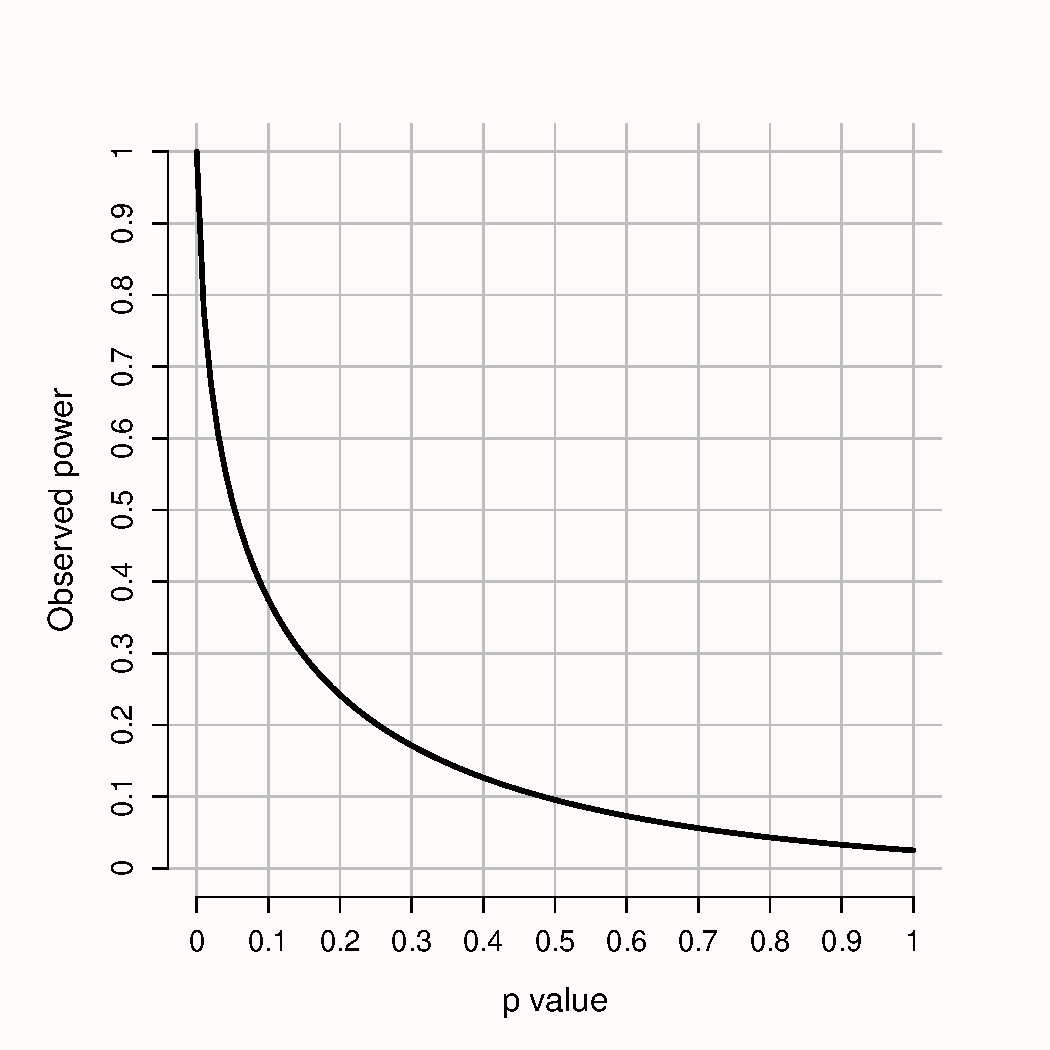
\includegraphics[width=1\textwidth,height=\textheight]{08-samplesizejustification_files/figure-pdf/fig-obs-power-plot-2-1.pdf}

}

\caption{\label{fig-obs-power-plot-2}\(\alpha\) = 0.05 且 n = 10
时,独立 t 检验的 p 值与检验力之间的关系}

\end{figure}

期刊编辑或审稿人可能会要求研究者报告事后检验力,以区分真阴性(确实没有效应)和假阴性(也就是
II 类错误,效应真实存在但未被发现)。但实际上事后检验力只是报告 p
值的另一种方式,报告事后检验力不足以解决编辑所提出的问题(Hoenig \&
Heisey, 2001; Lenth, 2007; Schulz \& Grimes, 2005; Yuan \& Maxwell,
2005)。为了得出有意义的效应确实不存在的结论,研究者应该进行等价检验,并设计一个高检验力的研究来验证感兴趣的最小效应不存在。或者,研究设计之初并没有确定感兴趣的最小效应量时,研究者可以报告灵敏度功效分析。

\hypertarget{sec-sequentialsamplesize}{%
\section{序列分析(Sequential
Analyses)}\label{sec-sequentialsamplesize}}

在序列设计中,利用先验检验力来衡量样本量是否合理是非常有效的。序列设计可以在数据收集过程中多次分析来控制错误率(例如,在收集了50、100和150个观测数据之后),与一次性的设计(fixed
design)相比,序列设计可以在一定程度上减少预期的平均样本量,因为一次性设计通常需要在收集大量数据后才进行数据分析(Proschan
et al., 2006; Wassmer \& Brannath, 2016)。序列设计有很长的历史(Dodge \&
Romig, 1929),产生了一些的演变,比如说,序列概率比检验 (Wald,
1945),序列贝叶斯因子(sequential Bayes factors)(Schönbrodt et al.,
2017) 以及和安全性检验(safe testing)(Grünwald et al.,
2019)。在这些方法中,如果边实验边分析数据,使用序列概率比检验最有效(Schnuerch
\& Erdfelder,
2020)。成组序列设计,即分批收集数据,在数据收集、误差控制和效应量估计的调整等方面更灵活
(Wassmer \& Brannath,
2016)。如果变量之间存在某种依存关系(dependecies),安全性检验的灵活性最佳
(ter Schure \& Grünwald, 2019)。

当效应量非常不确定时,或者当真正的效应量可能大于研究的最小效应量时,序列设计将非常有用(Lakens,
2014)。在这种情况下,如果效应量大于感兴趣的最小效应量,就可以提前结束数据收集,但如果需要的话,仍然可以继续收集到最大样本量。序列设计可以在假设检验过程中避免无效工作量,可以在确实存在效应(拒绝零假设)时停止收集数据,也可以在确实无效应(拒绝备择假设)时停止。成组序列设计是目前最广泛使用的序列分析方法,可以用rpact(Wassmer
\& Pahlke, 2019)或gsDesign(K. M. Anderson,
2014)进行计划和分析。在线应用程序可用于rpact:
https://rpact.shinyapps.io/public/ 和 gsDesign:
https://gsdesign.shinyapps.io/prod/

\hypertarget{ux5728ux4e0dux589eux52a0ux6837ux672cux91cfux7684ux60c5ux51b5ux4e0bux63d0ux9ad8ux68c0ux9a8cux529b}{%
\section{在不增加样本量的情况下提高检验力}\label{ux5728ux4e0dux589eux52a0ux6837ux672cux91cfux7684ux60c5ux51b5ux4e0bux63d0ux9ad8ux68c0ux9a8cux529b}}

提升研究价值最直接的方法是增加样本量。通常因为资源有限,所以在不增加样本量的情况下,探索不同的方法来提高检验力也很有价值。第一个选择是使用相关的方向性检验。研究者通常会做出方向性的预测,比如''我们预测X大于Y''。从逻辑上来说,由这个预测得出的统计检验是方向性(或单侧)的
t 检验。方向性检验会将 I
类错误率移动到分布尾部的一侧上,这会使得临界值变小,因此只需要较少的样本量就能获得相同的统计检验力。

虽然有一些关于方向性检验何时适用的讨论,都在用Neyman-Pearson对假设检验的观点来支持自己的想法
(Cho \& Abe,
2013),这使得(预注册的)方向性检验成为一种最直接的方法,既能提高检验能力,但也会加大预测风险。然而,在某些情况下,你可能没办法提出一个方向性问题。特别是在具有应用价值的研究中,尽管结果与预期方向相反,但检验结果是否能够拒绝零效应也很重要。例如,当你正在评估最近引入的一项教育干预措施,并预测该干预措施将提高学生的表现,你可能想要探究一下学生表现更差的可能性,以便能够建议学校放弃这项新的干预措施。在这种情况下,也可能以''不平衡''的方式分配错误率,例如,相比于积极方向,将更严格的错误率分配给消极方向(Rice
\& Gaines, 1994)。

在不增加样本量的情况下,增加检验力的另一种方法是提高检验的 α
水平,如折中检验力分析部分所述,显然,这增加了犯 I
类错误的概率。我们应当认真权衡犯任何一类错误的风险,这通常需要考虑零假设为真的先验概率(Cascio
\& Zedeck, 1983; Miller \& Ulrich, 2019; Mudge et al., 2012; Murphy et
al.,
2014)。如果你''必须''做出决定,或者想要提出一种观点,而你能收集到的数据又确实有限,那么无论是基于折中检验力分析或是成本-效益分析(cost-benefit
analysis),提高 α 水平都是合理的 (Baguley, 2004; Field et al., 2004)。

另一种被广泛推荐的提高研究检验力的方法是尽可能使用被试内设计。几乎在所有情况下,当研究者对组间差异感兴趣时,被试内设计需要的被试比被试间设计少。可以从
Maxwell et al. (2017)
给出的等式来解释样本量减少的原因。假设总体正态分布,一个两组的被试内设计(NW)的被试量与一个两组的被试间设计(NB)所需的被试量相关:

\[NW = \frac{NB (1-\rho)}{2}\]

被试间设计所需的被试量是被试内设计的 2
倍,因为在一个具有两种条件的被试内设计中,每个被试提供两个数据点。与被试间设计相比,在多大程度上减少样本量还取决于因变量之间的相关性(例如,控制组与实验组数据之间的相关性),这一点体现在方程的
(1-p) 部分。如果相关性为 0
,则被试内设计只需要被试间设计被试数量的一半(例如,被试内64名被试,被试间
128 名被试)。相关性越高,被试内设计的相对效益就越大,当相关性为负(高达
-1
)时,相对效益就会消失。特别是当被试内设计中的因变量是正相关时,基于可得的样本量,被试内设计将极大地提高检验力。尽可能使用被试内设计,但要权衡更高的检验力所带来的好处与被试内设计中产生的顺序效应或遗留效应(carryover
effect,即练习效应和疲劳效应)所带来的负面影响(Maxwell et al.,
2017)。你可以在这个在线应用程序中比较被试内和被试间设计:http://shiny.ieis.tue.nl/within\_between
对于多因素多水平的设计,可能很难给出完整的相关矩阵(即每对变量间的相关性所构成的矩阵)Lakens
\& Caldwell (2021)。在这些情况下,序列分析也许能够提供解决方案。

一般来说,变异越小,标准化效应量就越大(将原始效应除以较小的标准差),因此在样本量相同的情况下,检验力就越高。文献中提供了一些额外的建议(Allison
et al., 1997; Bausell \& Li, 2002; Hallahan \& Rosenthal, 1996),例如:

参与实验之前,如果需要对被试进行筛选,建议使用更高效的方法进行筛选。

将被试不均等地分配到不同条件(例如,控制组下的数据比实验组的数据更易收集)。

采用较低误差的可靠测量方法(Williams et al., 1995)。

巧妙使用预注册的协变量(Meyvis \& Van Osselaer, 2018)。

重要的是要考虑,减少数据变异的这些方法是否会损耗过多的外部效度。例如,在随机控制试次的意向性治疗分析(Intention-to-treat
analysis)中,不遵守协议的被试将被保留在分析中,这样研究的效应能准确地代表在人群中实施干预后所得到的效应,而不是只代表了那些完全遵守协议的人的干预效应(Gupta,
2011)。在减少变异和外部效度两方面上,其他研究领域也存在类似的权衡。

\hypertarget{sec-knowyourmeasure}{%
\section{了解你的测量方法}\label{sec-knowyourmeasure}}

虽然讨论标准化的效应量大小很方便,但如果研究者能够用原始(非标准化)分数来解释效应,并了解其测量的标准偏差,相对来说是更好的(Baguley,
2009; Lenth,
2001)。为了使学术界能够对实验数据的标准偏差有一个实际预期,同领域内的研究者使用相同效度的测量方式将更有益。这将提供更加可靠的信息,使得期望精确度的设计更容易,也能够在先验检验力分析中使用一个非标准化的感兴趣的最小效应量。

除了对标准偏差的了解之外,了解因变量之间的相关性也很重要(例如,因为一个因变量
t 检验的Cohen's \emph{d}\textsubscript{z}
依赖于均值之间的相关性)。在进行预测时,模型越复杂,就需要了解数据生成过程的更多方面。例如,在层级模型中,研究者需要了解变异的成分以进行检验力分析(DeBruine
\& Barr, 2021; Westfall et al.,
2014)。最后,研究所用测量方法的信度很重要(Parsons et al.,
2019),尤其是在参考一项已发表研究的效应量时,而你和它所使用的测量方法信度不同,或者同一测量方法用于不同的群体时,这时,不同群体之间的测量信度可能不同。随着开放数据的增加,通过以往研究数据来估计这些参数将会更容易。

如果我们计算样本的标准偏差,这个值是对总体真实值的估计。在小样本中,我们的估计值与真实值可能有较大差距,然而由于大数定律,随着样本量的增加,我们对标准偏差的估计将更加精确。由于样本标准差是一个不确定的估计值,所以我们可以围绕估计值计算出置信区间(Smithson,
2003),也可以设计小样本的预实验(pilot
study),得出可靠的标准偏差估计值。方差 \(\sigma^2\)
的置信区间如下公式所示,标准偏差的置信区间则为这些值的平方根:

\[(N - 1)s^2/\chi^2_{N-1:\alpha/2},(N - 1)s^2/\chi^2_{N-1:1-\alpha/2}\]

当参数存在不确定性时,研究者可以使用序列设计进行内部的预实验(internal
pilot study)(Wittes \& Brittain,
1990)。内部预实验的理念是,研究者为研究指定一个暂定的样本量,进行中期分析,使用内部预实验的数据来更新参数,如实验的方差,最后得出最终的样本量。只要对数据的中期考察是盲目的(例如,不考虑相关条件的信息),就可以根据新的方差估计结果对样本量进行调整,而不会对
I 类错误产生任何实际影响(Friede \& Kieser, 2006; Proschan,
2005)。因此,如果研究者想设计一个定性研究,其中 I 类和 II
类错误已经得到控制,但他们缺乏关于标准偏差的信息,内部预实验可能是一个值得考虑的方法(Chang,
2016)。

\hypertarget{ux7ea6ux5b9aux4fd7ux6210ux7684ux5143ux7ecfux9a8cux6cd5ux5219conventions-as-meta-heuristics}{%
\section{约定俗成的元经验法则(Conventions as
meta-heuristics)}\label{ux7ea6ux5b9aux4fd7ux6210ux7684ux5143ux7ecfux9a8cux6cd5ux5219conventions-as-meta-heuristics}}

即使研究者可能不会直接使用经验法则式的方法来确定研究中的样本量,但经验法则也会间接地在样本量规划中发挥作用。基于推断目标的样本量论证(如检验力分析、准确度或决策),都要求研究者确定
I 类和 II
类错误、精确度以及感兴趣的最小效应量的预期数值。尽管有时可以证实上述数值的合理性(例如,基于成本-效益分析),但这些数值的可靠程度可能需要更专门的研究来验证。这样更专门的研究可能很难实现,因为这些研究本身可能就不值得花钱(例如,用大多数同行认为保守的
α 水平进行研究,比基于成本-收益分析收集数据来确定所需 α
水平,所花费的更少)。所以在这些情况下,研究者倾向于使用惯例的数值。

当涉及到计算样本量所需的置信区间宽度、期望检验力或任何其他输入值时,透明且公开地报告如何使用经验法则或惯例(例如通过使用本文所附带的在线应用程序)非常重要。例如,通常在没有进行合理性论证的情况下,使用
5\% 的 Ⅰ 类错误和 80\%
的检验力实际上是同行所能接受的最小信息价值的一个较低的阈值(而对样本量进行合理性论证时,同行也可以接受更高的错误率)。重要的是我们需要认识到,这些数值不是固定的。期刊在投稿指南中可以任意规定一个他们所希望的更高效准确的信息价值(例如,Nature
Human Behavior杂志要求投稿的研究设计要达到 95\%
的统计检验力,我自己所在的部门要求研究者提交ERB提案,尽可能使研究设计达到
90\%
的统计检验力)。如果某研究者所报告的信息价值高于以往研究的最低值,应当给予一定鼓励。

在过去,一些领域已经改变了以往的惯例,比如现在在物理学中用 5σ
阈值来宣布一个发现,而不再使用 5\% 的 I
类错误。在其他领域,尚未有这种尝试获得成功的(例如,Johnson
(2013)。改进后的惯例应视具体情况而定,通过学会的学术会议来确定惯例可能更明智(Mullan
\& Jacoby,
1985)。学会会议在医学领域中很常见,并已被用于确定感兴趣的最小效应量(例如,Fried
et al.
(1993)。在许多研究领域,现行惯例都可以进行改进。例如,单项研究和元分析的默认
α 水平为 5\% 似乎很奇怪,可以想象,未来元分析的默认 α 水平将远低于 5\%
。在特定情况下,让大家更清楚什么样的输入值缺乏合理的缘由,这将会促使各个领域开始讨论该如何改进现行惯例。日后如果可能的话,在线应用程序将会链接到更好示例,并随之更新。

\hypertarget{ux5b9aux6027ux7814ux7a76ux4e2dux7684ux6837ux672cux91cfux89c4ux5212}{%
\section{定性研究中的样本量规划}\label{ux5b9aux6027ux7814ux7a76ux4e2dux7684ux6837ux672cux91cfux89c4ux5212}}

样本量规划对于定性研究来说也很重要。在定性研究中,样本量的规划应该基于如下的考虑:花费成本收集更多被试的数据但并不能产生更多信息了,之前的信息已经足以实现推理目标。这种观点的一种广泛应用被称为饱和,这意味着,新数据重复了早期的观测结果而没有添加新信息(Morse,
1995)。例如,假设我们问人们他们为什么养宠物,通过访谈,结果能得到几类原因,但在采访了20个人之后,没有新的原因分类出现,那么此时已经达到了饱和。定性研究还有其他的思想体系(philosophies)存在,并非所有思想体系存在饱和的问题。遗憾的是,还没有针对这些思想体系提出合适的样本量规划的方法(Marshall
et al., 2013)。

采样时,通常不是选择具有代表性的样本,而是选择一个包含足够多样化的被试样本,以便有效地达到饱和。Fugard和Potts
(2015)
展示了在定性研究中,如何对样本量进行更高效的规划,1)群体中存在的编码数量(例如,人们养宠物的原因数量),2)从单个信息源中得到编码的概率(例如,你采访某个人,他可能所提到的每个养宠原因的概率),3)你想要得到的每个编码的次数(即每个原因出现的频次)。他们在R中提供了一个基于二项分布的公式来计算所需样本量,以便获取所需编码的期望概率。

Rijnsoever (2017)
采用了一种更先进的方法,该方法也探讨了不同抽样策略的重要性。一般来说,相对于随机采样,有目的地从你所期望的样本中采样来获取信息将更加高效,但这需要你对预期的编码和每个编码的子群体都有很好的理解。有时我们也许能够确定,在采访某个信息源时至少会产生一个新的编码(例如,基于采访前的非正式沟通)。在定性研究中,一个好的样本量规划是基于:1)对总体(包括所有子集)的识别,2)对总体(子集)中编码数量的估计,3)在信息源中获得一个编码的概率,4)所使用的抽样策略。

\hypertarget{discussion}{%
\section{Discussion}\label{discussion}}

要设计一项内容丰富的研究,论证样本量的合理性是必不可少的步骤。根据数据收集的目标、可用的资源和统计分析的方法,有多种途径来证明研究样本量设置的合理性。所有这些方法的首要原则是:研究者应将他们所收集的信息价值与他们的推理目标联系起来。

在研究设计的样本量合理性论证过程中,有时会得出这样的结论:收集数据是不值得的,因为这项研究付出的成本并不能收获足够的信息价值。在某些情况下,不太可能有足够的数据来进行元分析(例如,因为大众对主题缺乏普遍的兴趣),这些信息将不会被用于做出决定或声明,且统计检验不允许你以合理的错误率来检验假设,也不允许你以足够的精确度来估计效应量。如果没有足够的理由去收集尽可能多的数据,那么无论如何进行这项研究都是在浪费时间和金钱(G.
W. Brown, 1983; Button et al., 2013; S. D. Halpern et al., 2002)。

越来越多的心理学家意识到,在过去的研究中,样本量往往太小,无法实现推断目标(Button
et al., 2013; Fraley \& Vazire, 2014; Lindsay, 2015; Sedlmeier \&
Gigerenzer,
1989)。随着越来越多的期刊开始要求论证样本量,一些研究者也将意识到他们需要收集比过去更多的样本量。这意味着研究者需要在资助提案中要求更多用于被试费的资金,或者需要更多的合作(Moshontz
et al.,
2018)。如果你认为你的研究问题很重要,但以你现有的资源无法回答这个研究问题,进而可以考虑与同行进行合作研究,共同寻求这个问题的答案。

论证样本量的合理性不应该被视为研究者在申请资助、通过伦理审查或发表手稿之前所需要克服的障碍。如果只是简单陈述样本量,而没有仔细地论证,那么会很难评估研究者收集的信息价值是否超过数据收集的成本。能够对样本量做出强有力的论证,意味着研究者知道他们想从研究中了解什么,并且能够设计出一项为科研问题提供丰富答案的研究。

\hypertarget{test-yourself-not-translated-yet}{%
\section{Test Yourself {[}Not Translated
Yet{]}}\label{test-yourself-not-translated-yet}}

\textbf{Q1}: A student has at most 2 months to collect data. They need
to pay participants for their participation, and their budget is limited
to 250 euro. They decide to collect all the participants they can in the
amount of time, and with the money they have available. What type of
sample size justification is this?

\begin{itemize}
\item
  \begin{enumerate}
  \def\labelenumi{(\Alph{enumi})}
  \tightlist
  \item
    Collecting the entire population\\
  \end{enumerate}
\item
  \begin{enumerate}
  \def\labelenumi{(\Alph{enumi})}
  \setcounter{enumi}{1}
  \tightlist
  \item
    A resource justification\\
  \end{enumerate}
\item
  \begin{enumerate}
  \def\labelenumi{(\Alph{enumi})}
  \setcounter{enumi}{2}
  \tightlist
  \item
    A heuristic\\
  \end{enumerate}
\item
  \begin{enumerate}
  \def\labelenumi{(\Alph{enumi})}
  \setcounter{enumi}{3}
  \tightlist
  \item
    No justification\\
  \end{enumerate}
\end{itemize}

\textbf{Q2}: What is the goal of an a-priori power analysis?

\begin{itemize}
\item
  \begin{enumerate}
  \def\labelenumi{(\Alph{enumi})}
  \tightlist
  \item
    Achieve a desired statistical power for the true effect size, and
    controlling the Type 1 error rate.\\
  \end{enumerate}
\item
  \begin{enumerate}
  \def\labelenumi{(\Alph{enumi})}
  \setcounter{enumi}{1}
  \tightlist
  \item
    Achieve a desired statistical power for an effect size of interest,
    and controlling the Type 1 error rate.\\
  \end{enumerate}
\item
  \begin{enumerate}
  \def\labelenumi{(\Alph{enumi})}
  \setcounter{enumi}{2}
  \tightlist
  \item
    Achieve a desired statistical power for the true effect size, and
    controlling the Type 2 error rate.\\
  \end{enumerate}
\item
  \begin{enumerate}
  \def\labelenumi{(\Alph{enumi})}
  \setcounter{enumi}{3}
  \tightlist
  \item
    Achieve a desired statistical power for an effect size of interest,
    and controlling the Type 2 error rate.\\
  \end{enumerate}
\end{itemize}

\textbf{Q3}: A researcher already knows the sample size they will be
able to collect. Given this sample size, they choose to compute equal
Type 1 and Type 2 error rates for an effect size of interest. This is
known as:

\begin{itemize}
\item
  \begin{enumerate}
  \def\labelenumi{(\Alph{enumi})}
  \tightlist
  \item
    An a-priori power analysis\\
  \end{enumerate}
\item
  \begin{enumerate}
  \def\labelenumi{(\Alph{enumi})}
  \setcounter{enumi}{1}
  \tightlist
  \item
    A sensitivity power analysis\\
  \end{enumerate}
\item
  \begin{enumerate}
  \def\labelenumi{(\Alph{enumi})}
  \setcounter{enumi}{2}
  \tightlist
  \item
    A post-hoc power analysis\\
  \end{enumerate}
\item
  \begin{enumerate}
  \def\labelenumi{(\Alph{enumi})}
  \setcounter{enumi}{3}
  \tightlist
  \item
    A compromise power analysis\\
  \end{enumerate}
\end{itemize}

\textbf{Q4}: Looking at the formula in the section `Increasing Power
Without Increasing the Sample Size'. which two factors contribute to the
fact that within subject designs can have much more power, with the same
number of participants, than between subject designs?

\begin{itemize}
\item
  \begin{enumerate}
  \def\labelenumi{(\Alph{enumi})}
  \tightlist
  \item
    The fact a participant contributes multiple observations, and the
    fact that effect sizes within individuals are typically larger than
    effect sizes between individuals.\\
  \end{enumerate}
\item
  \begin{enumerate}
  \def\labelenumi{(\Alph{enumi})}
  \setcounter{enumi}{1}
  \tightlist
  \item
    The fact a participant contributes multiple observations, and the
    effect of the correlation between measurements.\\
  \end{enumerate}
\item
  \begin{enumerate}
  \def\labelenumi{(\Alph{enumi})}
  \setcounter{enumi}{2}
  \tightlist
  \item
    The fact that order effects increase the effect size, and the effect
    of the correlation between measurements.\\
  \end{enumerate}
\item
  \begin{enumerate}
  \def\labelenumi{(\Alph{enumi})}
  \setcounter{enumi}{3}
  \tightlist
  \item
    The fact that order effects increase the effect size, and the fact
    that effect sizes within individuals are typically larger than
    effect sizes between individuals.\\
  \end{enumerate}
\end{itemize}

\textbf{Q5}: Which factors determine the minimal statistically
detectable effect?

\begin{itemize}
\item
  \begin{enumerate}
  \def\labelenumi{(\Alph{enumi})}
  \tightlist
  \item
    The power of the study\\
  \end{enumerate}
\item
  \begin{enumerate}
  \def\labelenumi{(\Alph{enumi})}
  \setcounter{enumi}{1}
  \tightlist
  \item
    The true effect size in the study\\
  \end{enumerate}
\item
  \begin{enumerate}
  \def\labelenumi{(\Alph{enumi})}
  \setcounter{enumi}{2}
  \tightlist
  \item
    The sample size and alpha level\\
  \end{enumerate}
\item
  \begin{enumerate}
  \def\labelenumi{(\Alph{enumi})}
  \setcounter{enumi}{3}
  \tightlist
  \item
    The observed effect size in the sample\\
  \end{enumerate}
\end{itemize}

\textbf{Q6}: All else equal, if you want to perform a study that has the
highest possible informational value, which approach to specifying the
effect size of interest is the best choice?

\begin{itemize}
\item
  \begin{enumerate}
  \def\labelenumi{(\Alph{enumi})}
  \tightlist
  \item
    Specify a smallest effect size of interest.\\
  \end{enumerate}
\item
  \begin{enumerate}
  \def\labelenumi{(\Alph{enumi})}
  \setcounter{enumi}{1}
  \tightlist
  \item
    Compute the minimal statistically detectable effect.\\
  \end{enumerate}
\item
  \begin{enumerate}
  \def\labelenumi{(\Alph{enumi})}
  \setcounter{enumi}{2}
  \tightlist
  \item
    Use an effect size estimate from a meta-analysis.\\
  \end{enumerate}
\item
  \begin{enumerate}
  \def\labelenumi{(\Alph{enumi})}
  \setcounter{enumi}{3}
  \tightlist
  \item
    Perform a sensitivity power analysis.\\
  \end{enumerate}
\end{itemize}

\textbf{Q7}: In an a-priori power analysis based on an empirical
estimate of the literature, which 2 issues are important to consider,
both when using an estimate from a meta-analysis, as from a single
study?

\begin{itemize}
\item
  \begin{enumerate}
  \def\labelenumi{(\Alph{enumi})}
  \tightlist
  \item
    Evaluate the risk of bias in the estimate, and evaluate the
    uncertainty in the effect size estimate.\\
  \end{enumerate}
\item
  \begin{enumerate}
  \def\labelenumi{(\Alph{enumi})}
  \setcounter{enumi}{1}
  \tightlist
  \item
    Evaluate the heterogeneity underlying the effect size estimate, and
    evaluate the similarity of the study/studies the estimate is based
    on with the study you plan to perform.\\
  \end{enumerate}
\item
  \begin{enumerate}
  \def\labelenumi{(\Alph{enumi})}
  \setcounter{enumi}{2}
  \tightlist
  \item
    Evaluate the risk of bias in the estimate, and evaluate the
    similarity of the study/studies the estimate is based on with the
    study you plan to perform.\\
  \end{enumerate}
\item
  \begin{enumerate}
  \def\labelenumi{(\Alph{enumi})}
  \setcounter{enumi}{3}
  \tightlist
  \item
    Evaluate the heterogeneity underlying the effect size estimate, and
    evaluate the uncertainty in the effect size estimate.\\
  \end{enumerate}
\end{itemize}

\textbf{Q8}: Imagine a researcher did not justify their sample size
before performing the study, and had no justification for the sample
size they choose. After submitting their scientific article to a journal
reviewers ask for a justification of the sample size. Of course, honesty
requires the authors to write down there was no justification, but how
can they still evaluate the informational value of the study for effect
sizes of interest?

\begin{itemize}
\item
  \begin{enumerate}
  \def\labelenumi{(\Alph{enumi})}
  \tightlist
  \item
    Perform an a-priori power analysis\\
  \end{enumerate}
\item
  \begin{enumerate}
  \def\labelenumi{(\Alph{enumi})}
  \setcounter{enumi}{1}
  \tightlist
  \item
    Perform a compromise power analysis\\
  \end{enumerate}
\item
  \begin{enumerate}
  \def\labelenumi{(\Alph{enumi})}
  \setcounter{enumi}{2}
  \tightlist
  \item
    Perform a sensitivity power analysis\\
  \end{enumerate}
\item
  \begin{enumerate}
  \def\labelenumi{(\Alph{enumi})}
  \setcounter{enumi}{3}
  \tightlist
  \item
    Perform a post-hoc or retrospective power analysis\\
  \end{enumerate}
\end{itemize}

\textbf{Q9}: Why can it be useful to consider the effect size
distribution of findings in a specific research area when evaluating the
informational value of the study you are planning?

\begin{itemize}
\item
  \begin{enumerate}
  \def\labelenumi{(\Alph{enumi})}
  \tightlist
  \item
    If your study can only reject effects that are so large that they
    are very unlikely to be observed in a specific research area,
    collecting the data will not teach us anything we do not already
    know.\\
  \end{enumerate}
\item
  \begin{enumerate}
  \def\labelenumi{(\Alph{enumi})}
  \setcounter{enumi}{1}
  \tightlist
  \item
    You can use this information to design a study that has high power
    for the smallest effect size that is observed in a specific
    literature, which will lead to a study with high informational
    value.\\
  \end{enumerate}
\item
  \begin{enumerate}
  \def\labelenumi{(\Alph{enumi})}
  \setcounter{enumi}{2}
  \tightlist
  \item
    You can use this information to design a study that has high power
    to detect the median effect size in this literature, which will lead
    to a study with high informational value.\\
  \end{enumerate}
\item
  \begin{enumerate}
  \def\labelenumi{(\Alph{enumi})}
  \setcounter{enumi}{3}
  \tightlist
  \item
    You can use this information to design a study that has high power
    to reject the median effect size in this literature, which will lead
    to a study with high informational value.\\
  \end{enumerate}
\end{itemize}

\textbf{Q10}: Why is it nonsensical to ask researchers to perform a
post-hoc or retrospective power analysis, where the observed effect size
and the collected sample size is used to calculate the statistical power
of a test, when a non-significant finding is observed?

\begin{itemize}
\item
  \begin{enumerate}
  \def\labelenumi{(\Alph{enumi})}
  \tightlist
  \item
    Post-hoc power analyses are always based on assumptions, and
    therefore, when the assumptions are wrong, the post-hoc power
    analysis will not be informative.\\
  \end{enumerate}
\item
  \begin{enumerate}
  \def\labelenumi{(\Alph{enumi})}
  \setcounter{enumi}{1}
  \tightlist
  \item
    Due to the relationship between post-hoc power and a \emph{p}-value,
    whenever an effect is non-significant, post-hoc power will be low,
    so the post-hoc power analysis does not provide any useful
    additional information.\\
  \end{enumerate}
\item
  \begin{enumerate}
  \def\labelenumi{(\Alph{enumi})}
  \setcounter{enumi}{2}
  \tightlist
  \item
    A post-hoc power analysis is mathematically identical to a
    sensitivity power analysis for a specific effect size estimate, and
    it is better to plot power for a range of effect sizes, than for a
    specific value.\\
  \end{enumerate}
\item
  \begin{enumerate}
  \def\labelenumi{(\Alph{enumi})}
  \setcounter{enumi}{3}
  \tightlist
  \item
    The question is whether a non-significant effect is a true negative,
    or a false negative, and the risk of these errors should be
    controlled in advance through an a-priori power analysis, not after
    the data is collected through a post-hoc power analysis.\\
  \end{enumerate}
\end{itemize}

\textbf{Q11}: Researchers should not perform a post-hoc power analysis.
There are two solutions, one that can be implemented when designing a
study, and one when interpreting a non-significant result after the data
is in. Which solution can be implemented when the data is in?

\begin{itemize}
\item
  \begin{enumerate}
  \def\labelenumi{(\Alph{enumi})}
  \tightlist
  \item
    Evaluate the accuracy of the effect size estimate, or perform a
    sensitivity power analysis.\\
  \end{enumerate}
\item
  \begin{enumerate}
  \def\labelenumi{(\Alph{enumi})}
  \setcounter{enumi}{1}
  \tightlist
  \item
    Plan a study to have high power for an equivalence test, or perform
    a sensitivity power analysis.\\
  \end{enumerate}
\item
  \begin{enumerate}
  \def\labelenumi{(\Alph{enumi})}
  \setcounter{enumi}{2}
  \tightlist
  \item
    Evaluate the accuracy of the effect size estimate, or perform a
    compromise power analysis.\\
  \end{enumerate}
\item
  \begin{enumerate}
  \def\labelenumi{(\Alph{enumi})}
  \setcounter{enumi}{3}
  \tightlist
  \item
    Plan a study to have high power for an equivalence test, or perform
    a compromise power analysis.\\
  \end{enumerate}
\end{itemize}

\textbf{Q12}: What is a way/are ways to increase the statistical power
of a test, without increasing the sample size?

\begin{itemize}
\item
  \begin{enumerate}
  \def\labelenumi{(\Alph{enumi})}
  \tightlist
  \item
    Perform a one-sided test instead of a two-sided test.\\
  \end{enumerate}
\item
  \begin{enumerate}
  \def\labelenumi{(\Alph{enumi})}
  \setcounter{enumi}{1}
  \tightlist
  \item
    Increase the alpha-level of the test.\\
  \end{enumerate}
\item
  \begin{enumerate}
  \def\labelenumi{(\Alph{enumi})}
  \setcounter{enumi}{2}
  \tightlist
  \item
    Use measures with higher (compared to lower) error variance.\\
  \end{enumerate}
\item
  \begin{enumerate}
  \def\labelenumi{(\Alph{enumi})}
  \setcounter{enumi}{3}
  \tightlist
  \item
    All of the other answer options are correct.\\
  \end{enumerate}
\end{itemize}

\hypertarget{open-questions}{%
\subsection{Open Questions}\label{open-questions}}

\begin{enumerate}
\def\labelenumi{\arabic{enumi}.}
\item
  Why are resource constraints, if not the primary justification, always
  a secondary justification (if it is not possible to collect data from
  the entire population)?
\item
  What is the goal of an a-priori power analysis, and why is the goal
  not to achieve a desired Type 2 error rate for the true effect size?
\item
  Which factors determine the Minimal Statistically Detectable Effect,
  and why can it be useful to compute it for a study you are planning to
  perform?
\item
  What is a benefit of planning for precision, given that the effect
  size is typically unknown (and might even be 0). Which aspect of the
  decisions that need to be made when planning for precision is most
  difficult to justify?
\item
  What is a problem of using heuristics as the basis of a sample size
  justification?
\item
  It seems counter-intuitive to have a `no justification' category in a
  chapter on sample size justification, but why is it important to
  explicitly state there was no justification?
\item
  From all effect sizes that might be related to the inferential goal in
  a study, which of the 6 categories in
  Table~\ref{tbl-table-effect-eval} is the best approach (if it can be
  specified)?
\item
  Why can't you simply take an effect size estimate from a meta-analysis
  as the basis of an a-priori power analysis for a related study?
\item
  Why can't you simply take an effect size estimate from a single study
  as the basis of an a-priori power analysis for a related study?
\item
  What is the goal in a compromise power analysis?
\item
  Why is `post-hoc' or `retrospective' power not a useful way to draw
  inferences about non-significant results?
\item
  When would you perform a sensitivity power analysis?
\item
  How can the statistical power of a study be increased, without
  increasing the sample size?
\item
  Why can it be beneficial to use a within-design compared to a
  between-design (where possible)?
\end{enumerate}

\bookmarksetup{startatroot}

\hypertarget{equivalencetest}{%
\chapter{等价检验和区间假设检验}\label{equivalencetest}}

大多数学术研究旨在检验对某个效应或差异是否存在的假说。新的干预措施有效吗?两个变量之间有关系吗?这些研究通常采用零假设显著性检验进行分析。当观察到具有统计学意义上显著的\emph{p}值时,这个零假设便可被拒绝。同时,研究者可以在承认最大错误率的前提下声称干预有效,或两个变量之间存在关联。但是,如果\emph{p}值在统计意义上不显著,研究者往往会得出一个逻辑上不正确的结论:那就是他们基于\emph{p}
> 0.05的结果而得出效应不存在的结论。

打开你正在写的论文的结果部分,或者你最近读过的某篇论文的结果部分。搜索''\emph{p}
\textgreater0.05'',仔细观察你或这位学者得出的结论(在结果部分,但也请观察他们在讨论部分的说法)。如果你看到''没有效应''或''变量之间没有关联''的结论,那么你就发现了一个典型案例,即研究者忽略了\emph{缺乏证明并不意味着不存在}(Altman
\& Bland,
1995)。一个不显著的结果本身只是告诉我们不能拒绝零假设而已。在观察到\emph{p}
>0.05之后,``效应真的为零吗?''成为了值得思索的问题,但零假设显著性检验的\emph{p}
值却不能回答这个问题。因此,在得到\emph{p}>0.05后,可以将是否存在效应这一问题的答案视为''未定论''(\href{https://en.wikipedia.org/wiki/Mu_(negative)\#Non-dualistic_meaning}{mu}),即一种非二元回答,不是''是'',不是''否'',也不是''未提出问题''。总之,仅基于\emph{p}>0.05,并无法证明是否存在有意义的效应。

在许多情况下,研究者都应该对是否存在有意义的效应感兴趣。举个例子来说,证明可能成为混淆变量的因素在两个组别内没有差异是很重要的(例如,在积极情绪和消极情绪的实验操纵下,疲劳这一混淆变量不会影响当下的实验操纵)。研究者可能想知道两种干预措施是否同样有效,尤其是当新的干预措施成本更低或更加省力(例如,线上诊疗和线下诊疗一样有效吗?)。或者,在某些情况下我们会想证明效应不存在,比如理论模型预测效应不存在,或当我们认为之前发表的研究是假阳性的,我们会希望通过重复研究证明效应不存在(Dienes,
2014)。然而,如果你问研究者是否设计过旨在证明效应不存在的研究,比如研究假设为两种条件下没有差异,许多人会说他们从未设计过这种为了验证效应量为0的研究。研究者几乎总是猜想差异是存在的,原因之一可能是许多人甚至不知道如何从统计学上为效应量为0提供支持,因为他们没有接受过等价检验相关训练。

证明一个效应大小''正好''为零是永远不可能的。即便你从世界每个人那里收集数据,所得到的任
意一项研究的效应量都会在0左右随机变化------对于任何有限的样本来说,你最终可能都将得到非常接近但不完全为0的平均数差异。Hodges
\& Lehmann (1954)
是第一个讨论检验两个群体是否具有相同均值这一统计问题的人。他们建议(第264页):``检验两组的均值差异不超过特定数值,用来在实际操作中表示最小差异''。Nunnally
(1960)
同样提出了一个''固定增量''的假设,即研究者将观察到的效应与一个被认为太小而没有意义的数值范围进行比较。定义一个数值范围,范围内的值在实际意义上代表没有效应,此范围就被称为\textbf{等价范围}
(Bauer \& Kieser, 1996) 或\textbf{实际等价区域} (Kruschke,
2013)。等价范围应提前规定,并需要仔细考虑最小感兴趣区。

尽管研究者一再试图在社会科学领域中引入针对等价范围的检验 (Cribbie et
al., 2004; Hoenig \& Heisey, 2001; Levine et al., 2008; Quertemont,
2011; J. L. Rogers et al., 1993),
但这种统计方法直到最近才流行起来。在可重复性危机期间,研究者们在进行重复研究时需寻找用于解释无效结果的工具。研究者们希望在重复他们怀疑是假阳性的研究结论时,能够提出无效结果的声明,并有一定的证据给予支持。一个著名的例子是Daryl
Bem对前认知的研究,该研究表面上证明了被试能够预测未来(Bem,
2011)。等价检验作为一种统计方法被提出,用于回答观察到的效应量是否足够小到无法重复得出前人的研究结论(S.
F. Anderson \& Maxwell, 2016; Lakens, 2017; Simonsohn,
2015)。研究者会指定最小感兴趣区(例如0.5的效应量,即对于双侧检验来说,是在-0.5到0.5范围之外的任何值),并检验是否可以拒绝比这个范围更极端的效应。如果是这样,他们可以拒绝那些被认为足够大而有意义的效应的存在。

人们可以将\textbf{零效应的原假设(nil null
hypothesis)}与\textbf{非零效应的原假设(non-nil null
hypothesis)}区分开来,其中零效应的原假设是效应正好为0,非零效应的原假设是除0之外的任何其他效应,例如比最小感兴趣区更极端的效应(Nickerson,
2000)。正如尼克森所写:

\begin{quote}
这是一个很重要的区分,特别是当涉及到对NHST优缺点的争议时。有些批评针对零效应的原假设很有用,但在非零效应的原假设的情境下,由于后者更为宽泛,有时那些批评并不那么具有建设性。
\end{quote}

等价检验是\textbf{区间假设检验}的一种具体实现形式,它不是针对零效应的原假设进行检验(即,效应量为0的\textbf{零效应的原假设}),而是针对非零效应的原假设的某个区间进行检验(即,\textbf{非零假设的原假设})。其实在针对零假设显著性检验的局限性而提出的改进建议中,最广泛出现的就是使用区间假设检验中的范围检验来代替效应为0的零假设检验(Lakens,
2021)。为了说明这种差异,Figure~\ref{fig-intervaltest}
中的图A显示了双侧零效应的原假设检验结果,检验效应为0的原假设是否能被拒绝。图B为区间假设检验,检验效应落在0.5-2.5之间时,检验能否拒绝小于0.5或大于2.5的值。图C为等价检验,它基本上与区间假设检验相同,但效应落在0左右的范围内,其值被认为太小而没有意义的效应。

\begin{figure}

{\centering 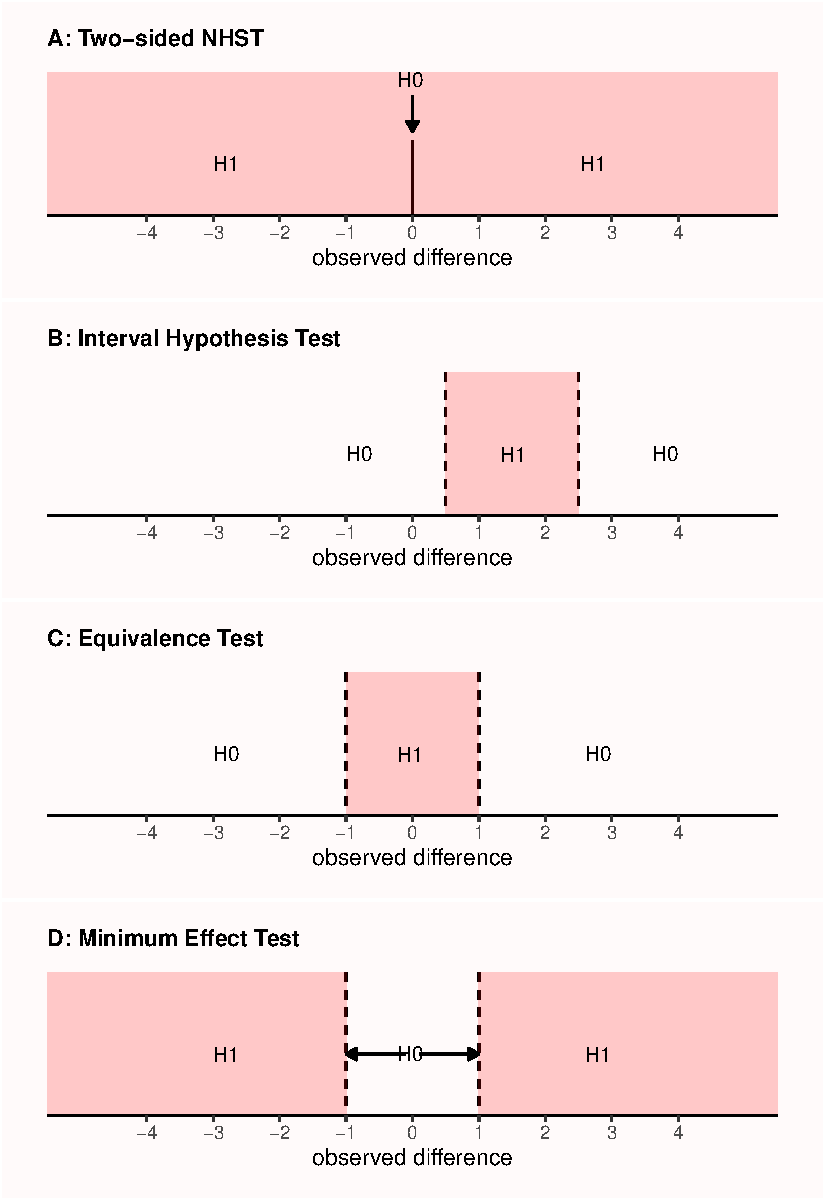
\includegraphics[width=1\textwidth,height=\textheight]{09-equivalencetest_files/figure-pdf/fig-intervaltest-1.pdf}

}

\caption{\label{fig-intervaltest}双侧零假设检验 (A), 区间假设检验 (B),
等价检验 (C) 以及最小效应量检验 (D).}

\end{figure}

将等价检验进行翻转,意味着研究者设计了一项研究来拒绝比最小感兴趣区还小的那些值,这被称为\textbf{最小效应量检验}(Murphy
\& Myors,
1999)。研究者可能不仅想要拒绝一个效应为0的假设(如零假设显著性检验),而且也想拒绝那些太小而没有意义的效应区间。在其他条件相同的情况下,相比于那些想拒绝0效应假设的研究,旨在拒绝最小效应区间并具有高统计检验力的研究则需要更多的观测值,因为后者的置信区间需要拒绝的值更接近观测到的效应量(例如,0.1而不是0),置信区间会变得更窄,这就需要更多的观测值。

与零假设检验相比,最小效应量检验的一个好处是在统计显著性和实际显著性之间没有区别。由于检验值被选择来表示最小感兴趣效应,无论何时被拒绝,这种影响在统计上和实际上都是显著的(Murphy
et al.,
2014)。最小效应量检验的另一个好处是,在社会科学领域的相关研究中,变量通常通过因果结构相互联系,导致变量之间存在真实但实际上我们并不感兴趣的非零相关性,这被称为''混杂因素''(crud
factor)(Meehl, 1990; Orben \& Lakens,
2020)。由于0效应在大型相关数据集中可能不会成立,因此拒绝零效应的原假设并不是一个严格的检验。即使假设不正确,0效应的假设也可能因''混杂因素''而被拒绝。因此一些研究者建议针对\emph{r}
=
0.1的最小效应进行检验,由于变量之间在理论上不相关,低于该阈值的相关性将非常常见(Ferguson
\& Heene, 2021)。

图@fig-intervaltest
表示了双侧检验,但做单侧检验通常更直观、更合乎逻辑。例如,最小效应量检验的目标是拒绝小于0.1的效应,而等价检验的目标是拒绝大于0.1的效应。与其指定范围的上限和下限,不如为单侧检验指定一个值。单侧非零效应的原假设检验的一种变式被称为\textbf{非劣效性检验},它检验效应是否大于等价范围的下限。例如,当一种新的干预措施不应该明显比现有的干预措施差,但可能会差一点点时,就可以进行这样的测试。例如,如果新的干预措施和现有的干预措施之间的差异不小于-0.1,并且小于-0.1的效应可以被拒绝,则可以得出结论,效果是非劣效的(Mazzolari
et al., 2022; Schumi \& Wittes,
2011)。我们发现,将零效应的原假设扩展到非零效应的原假设可以让研究者提出可能更有趣的问题。

\hypertarget{ux7b49ux4ef7ux68c0ux9a8c}{%
\section{等价检验}\label{ux7b49ux4ef7ux68c0ux9a8c}}

等价检验最早是在药物学中发展起来的(Hauck \& Anderson, 1984; Westlake,
1972),后来正式成为等价检验的\textbf{双单侧检验(TOST)}方法(Schuirmann,
1987; Seaman \& Serlin, 1998; Wellek,
2010)。TOST程序需要进行两次单侧检验,以检验观察到的数据是否出乎意料地大于等价下限(\(\Delta_{L}\)),
或者出乎意料地小于等价上限(\(\Delta_{U}\)):

\[
t_{L} = \frac{{\overline{M}}_{1} - {\overline{M}}_{2} - \Delta_{L}}{\sigma\sqrt{\frac{1}{n_{1}} + \frac{1}{n_{2}}}}
\]

和

\[
t_{U} = \frac{{\overline{M}}_{1} - {\overline{M}}_{2}{- \Delta}_{U}}{\sigma\sqrt{\frac{1}{n_{1}} + \frac{1}{n_{2}}}}
\]

其中\textbf{M}表示每个样本的平均值,\textbf{n}是样本量,σ是合并的标准偏差:

\[
\sigma = \sqrt{\frac{\left( n_{1} - 1 \right)\text{sd}_{1}^{2} + \left( n_{2} - 1 \right)\text{sd}_{2}^{2}}{n_{1} + \ n_{2} - 2}}
\]

如果这两个单侧检验都是显著的,我们就可以拒绝接受存在足够大而有意义的效应。这些公式与统计量\emph{t}的一般公式十分相似。NHST
\emph{t}检验和TOST程序之间的区别在于,NHST
\emph{t}检验从组别之间的平均差中减去了等价下限和等价上限(在正常的\emph{t}检验中,我们将平均差与0进行比较,因此∆从公式中剔除,因为它是0)。

要进行等价检验,你不需要学习任何新的统计检验,因为它只是针对不同于0的值进行的众所周知的t检验。但令人惊讶的是,使用\emph{t}检验进行等价检验并没有像在零假设显著性检验中使用\emph{t}检验那般进行同步教学,因为有迹象表明,这可以防止对\emph{p}值的常见误解(Parkhurst,
2001)。让我们来看一个使用TOST程序进行等价检验的例子。

在一项研究中,研究者通过让被试搬运沉重的盒子来操纵疲劳程度,并希望确保这种操纵不会无意中改变被试的情绪。研究者评估了这两种情况下的积极情绪和消极情绪,并希望能够声称积极情绪在两种情况下没有差异。让我们假设实验性疲劳条件下的积极情绪(\(m_1\)
= 4.55, \(sd_1\) = 1.05, \(n_1\) = 15)与控制组条件下的情绪(\(m_2\) =
4.87, \(sd_2\) = 1.11, \(n_2\) =
15)没有差异。为此,研究者得出结论:``不同条件下的情绪没有差异,\emph{t}=-0.81,\emph{p}=.42''。当然,不同条件下的情绪确实不同,因为4.55-4.87=-0.32。而这种说法是指两种情绪的差异\emph{无意义},如果要以正确的方式得出这样的结论,我们首先需要指定什么程度的情绪差异才能被视为是有意义的。目前,我们假设,研究者认为小于半个刻度点(即0.5)的效应都太小,因而没有意义。我们现在检验观察到的-0.32的平均差异是否足够小,以便我们可以去拒绝大到需要重视的效应的存在。

TOSTER软件包(最初由我创建,但最近由\href{https://aaroncaldwell.us/}{Aaron
Caldwell}重新设计)可用于绘制两个\emph{t}分布及其临界区域的图表,这将指示我们何时可以拒绝小于-0.5和大于0.5的效应。我们可能需要一些时间来习惯这样一种想法,即我们拒绝的值比等价边界更极端。在任何假设检验中,始终尝试提问:检验可以拒绝哪些值?在零效应的原假设中,我们可以拒绝效应为0的假设,在下图的等价检验中,可以拒绝低于-0.5和高于0.5的值。在图
Figure~\ref{fig-tdistequivalence}
中,我们可以看到两个\emph{t}分布集中在指定等价范围的上限和下限(-0.5和0.5)。

\begin{figure}

{\centering 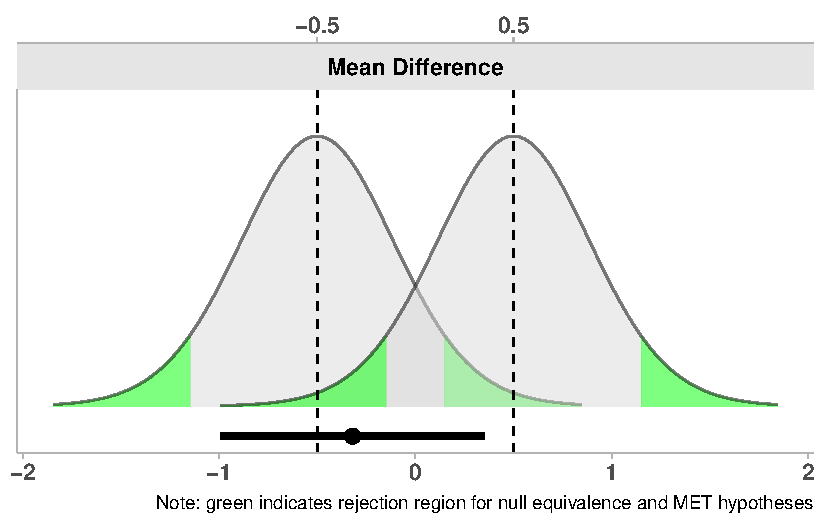
\includegraphics[width=1\textwidth,height=\textheight]{09-equivalencetest_files/figure-pdf/fig-tdistequivalence-1.pdf}

}

\caption{\label{fig-tdistequivalence}在用于对-0.5 和 0.5
进行两次单侧检验的 \emph{t} 分布下绘制的均值差以及其置信区间。}

\end{figure}

在这两条曲线之下,我们看到一条横线表示 -0.99
至0.35的置信区间,线上的一个点表示观察到的
-0.32的平均差异。让我们先看看左边的曲线。我们在尾部看到绿色高亮的区域,该区域显示了哪些平均差异将非常极端,足以在统计上拒绝-0.5的效应。我们所得到的-0.32的平均差异非常接近-0.5,如果只看左边的分布,均值差离-0.5还不够远,远到足以落在表明所得差异何时具有统计学意义的绿色区域。我们还可以使用TOSTER包进行等价检验,并查看结果。

\begin{Shaded}
\begin{Highlighting}[]
\NormalTok{TOSTER}\SpecialCharTok{::}\FunctionTok{tsum\_TOST}\NormalTok{(}\AttributeTok{m1 =} \FloatTok{4.55}\NormalTok{, }
                  \AttributeTok{m2 =} \FloatTok{4.87}\NormalTok{, }
                  \AttributeTok{sd1 =} \FloatTok{1.05}\NormalTok{, }
                  \AttributeTok{sd2 =} \FloatTok{1.11}\NormalTok{,}
                  \AttributeTok{n1 =} \DecValTok{15}\NormalTok{, }
                  \AttributeTok{n2 =} \DecValTok{15}\NormalTok{, }
                  \AttributeTok{low\_eqbound =} \SpecialCharTok{{-}}\FloatTok{0.5}\NormalTok{, }
                  \AttributeTok{high\_eqbound =} \FloatTok{0.5}\NormalTok{)}
\end{Highlighting}
\end{Shaded}

\begin{verbatim}

Welch Modified Two-Sample t-Test

The equivalence test was non-significant, t(27.91) = 0.456, p = 3.26e-01
The null hypothesis test was non-significant, t(27.91) = -0.811, p = 4.24e-01
NHST: don't reject null significance hypothesis that the effect is equal to zero 
TOST: don't reject null equivalence hypothesis

TOST Results 
                 t    df p.value
t-test     -0.8111 27.91   0.424
TOST Lower  0.4563 27.91   0.326
TOST Upper -2.0785 27.91   0.023

Effect Sizes 
               Estimate     SE              C.I. Conf. Level
Raw             -0.3200 0.3945 [-0.9912, 0.3512]         0.9
Hedges's g(av)  -0.2881 0.3930 [-0.8733, 0.3021]         0.9
Note: SMD confidence intervals are an approximation. See vignette("SMD_calcs").
\end{verbatim}

在''t检验''一行中,输出结果显示了传统零效应的原假设的显著性检验(我们已经知道这在统计学上并不显著:\emph{t}=0.46,p=0.42。就像R中的默认\emph{t}检验一样,tsum\_TOST函数在默认情况下会计算Welch's
\emph{t}检验(而不是Student's
\emph{t}检验),这是一个更好的默认值(Delacre et al.,
2017),但你可以通过添加\texttt{var.equal\ =\ TRUE}作为函数的参数来请求进行Student's
\emph{t}检验。

我们还看到TOST
Lower所示的检验。这是第一次单侧检验,检验我们是否可以拒绝低于-0.5的效应。从检验结果来看,情况并非如此:\emph{t}=0.46,\emph{p}=0.33。这是一个普通的\emph{t}检验,只是针对-0.5的效应。因为我们不能拒绝比-0.5更极端的差异,所以可能存在我们认为有意义的差异(例如,-0.60的差异)。当我们观察等价范围上限(0.5)的单侧检验时,我们可以从统计学上拒绝大于0.5的情绪效应的存在,正如在TOST
upper行中我们看到的\emph{t}=-2.08,\emph{p}=0.02。因此,我们的最终结论是,即使我们可以根据观察到的-0.32的平均差异来拒绝比0.5更极端的效应,我们也不能拒绝比-0.5更极端的效应。因此,我们不能完全拒绝有意义的情绪效应的存在。由于数据不允许我们声称效应与0有所不同,也不允许我们说效应太小而无关紧要(基于-0.5到0.5的等价范围),因此数据是\textbf{不确定}的。我们无法区分Ⅱ类错误(存在效应,但在这项研究中,我们只是没有检测到它)或真正的阴性(确实没有足够大到要去重视的效应)。

请注意,由于我们未能拒绝针对等价下限的单侧检验,因此仍有可能存在足够大以至于被认为是有意义的真实效应量。这种说法是正确的,即使我们观察到的效应大小(-0.32)比-0.5的等价边界更接近于零。有人可能认为,所得到的效应大小需要比等价边界更极端(即\textless-0.5或\textgreater0.5),这样才有可能存在一个大到足以被认为有意义的效应。但这并不是必须的。90\%的置信区间说明了不能拒绝低于-0.5的某些值。正如我们预期所示,从长远来看,90\%的置信区间捕捉到了真实的总体参数,真实的效应大小完全有可能比-0.5更极端。而且,这种效应甚至可能比这个置信区间捕获的值更极端,因为在10\%的概率下,计算的置信区间不包含真实的效应量。因此,当我们不能拒绝最小感兴趣区时,我们扔保留了存在效应的可能性。如果我们可以拒绝零效应的原假设,但不能拒绝比等价边界更极端的值,那么我们可以声称效应存在,并且它可能足够大,大到有意义。

降低效应不确定概率的一种方法是收集充分的数据。让我们想象一下,研究者并没有在每种情况下只收集15名被试,而是收集了200名被试。除此之外,他们观察到的数据完全相同。正如\protect\hyperlink{confint}{confidence
intervals}一章中所解释的,随着样本量的增加,置信区间变得越来越窄。为了使TOST等价检验能够拒绝等价范围的上限和下限,置信区间需要完全落在等价范围内。在图
Figure~\ref{fig-ciequivalence1} 中,我们看到了与图
Figure~\ref{fig-tdistequivalence}
相同的结果,但现在如果我们收集了200个数据。由于样本量较大,置信区间比我们收集15名被试时更窄。我们看到,观察到的平均差周围的90\%置信区间现在排除了等价上限和等价下限。这意味着我们现在可以拒绝等价范围之外的效应(尽管很勉强,因为对等价下限的单侧检验仅具有统计学意义,\emph{p}=0.048)。

\begin{verbatim}

Welch Modified Two-Sample t-Test

The equivalence test was significant, t(396.78) = 1.666, p = 4.82e-02
The null hypothesis test was significant, t(396.78) = -2.962, p = 3.24e-03
NHST: reject null significance hypothesis that the effect is equal to zero 
TOST: reject null equivalence hypothesis

TOST Results 
                t    df p.value
t-test     -2.962 396.8   0.003
TOST Lower  1.666 396.8   0.048
TOST Upper -7.590 396.8 < 0.001

Effect Sizes 
               Estimate    SE               C.I. Conf. Level
Raw             -0.3200 0.108 [-0.4981, -0.1419]         0.9
Hedges's g(av)  -0.2956 0.104 [-0.4605, -0.1304]         0.9
Note: SMD confidence intervals are an approximation. See vignette("SMD_calcs").
\end{verbatim}

\begin{figure}

{\centering 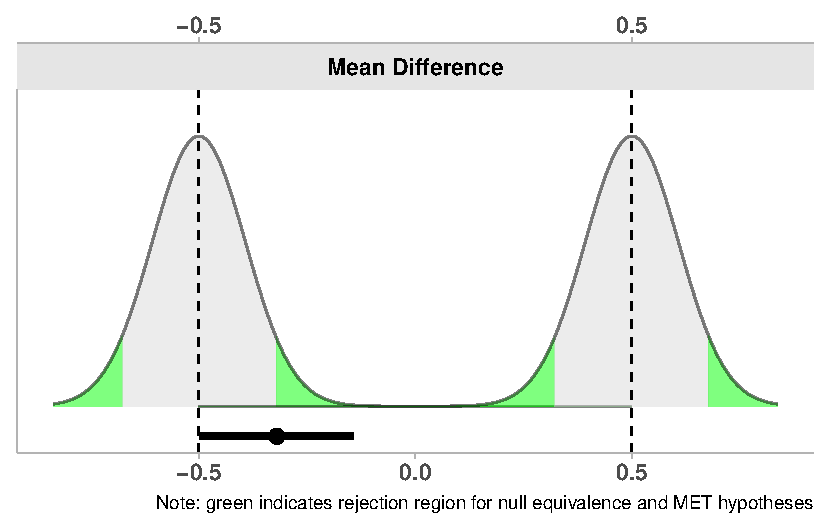
\includegraphics[width=1\textwidth,height=\textheight]{09-equivalencetest_files/figure-pdf/fig-ciequivalence1-1.pdf}

}

\caption{\label{fig-ciequivalence1}等效范围为-0.5和0.5的等效性检验的平均差及其置信区间}

\end{figure}

在图 Figure~\ref{fig-ciequivalence2}
中,我们看到了相同的结果,但现在可视化为置信密度图(Schweder \& Hjort,
2016),这是置信度分布的图形总结。置信密度图允许你查看哪些效应可以通过不同的置信区间宽度来拒绝。我们看到绿色区域的边界(对应于90\%的置信区间)落在等价边界内。因此,等价检验在统计学上是显著的,我们可以在统计学上拒绝存在等价范围之外的效应。我们还可以看到,95\%的置信区间排除了0,因此,传统的零假设显著性检验也具有统计学意义。

\begin{figure}

{\centering 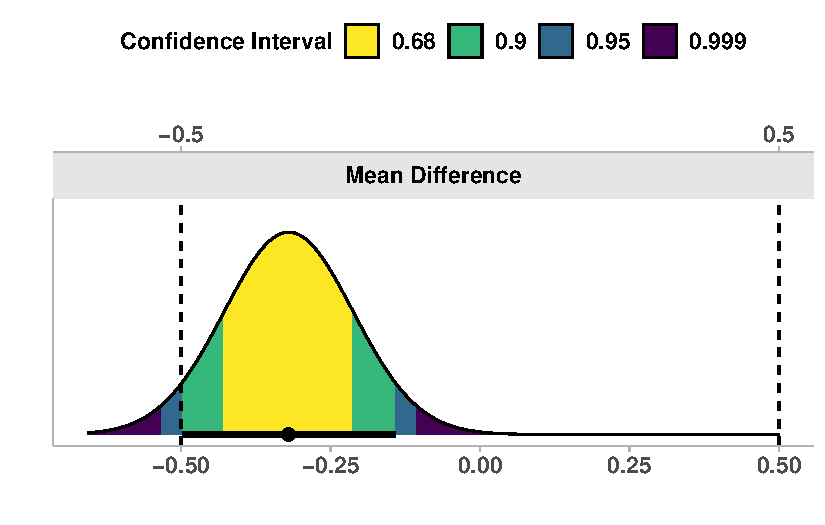
\includegraphics[width=1\textwidth,height=\textheight]{09-equivalencetest_files/figure-pdf/fig-ciequivalence2-1.pdf}

}

\caption{\label{fig-ciequivalence2}等效范围为-0.5和0.5的等效性检验的平均差及其置信区间}

\end{figure}

换句话说,零假设检验和等价检验都产生了显著的结果。这意味着我们可以声称,所观察到的效应在统计学上与0不同,并且在统计上,该效应小于我们在指定的-0.5到0.5的等效区间时认为的大到足够重要的效应。这说明了将等价检验和零效应的原假设相结合可以防止我们误将具有统计学意义的效应当成实际上显著的效应。在这种情况下,有200名被试,我们可以拒绝一个为0的效应,但这个效应(如果有的话)没有大到是有意义的。

\hypertarget{ux62a5ux544aux7b49ux4ef7ux68c0ux9a8c}{%
\section{报告等价检验}\label{ux62a5ux544aux7b49ux4ef7ux68c0ux9a8c}}

在报告等价检验时,通常只报告两个单侧检验中产生较高\emph{p}值的检验。因为两个单侧检验都需要具有统计学意义,才能在等价检验中拒绝零假设(即存在足够大的效应),所以当两个假设检验中较大的一个拒绝等价边界时,另一个检验也会拒绝。与零假设显著性检验不同的是,报告等价检验的标准化效应量并不常见,但在某些情况下,研究者可能想讨论当前效应与等价边界初始度量的差距有多远。防止例如声称'没有效应'、效应'不存在'、真实效应量为'0'这样错误的解释,或两组数据''相似''或''可比''这样模糊的口头描述。显著的等价检验会拒绝比等价边界更极端的效应。较小的真实效应没有被拒绝,因此仍然有可能存在真实效应。因为TOST程序是一种基于\emph{p}值的频率检验,所以也应该防止所有其他的\protect\hyperlink{misconceptions}{对\emph{p}值的误解}。

在总结等价检验的主要结果时,例如在摘要中,始终要报告数据所检验的等价范围。比方说,等价边界为\emph{d}
-0.9至0.9,那么'基于等价检验,我们认为有意义的效应不存在'这个结论与等价边界为\emph{d}
= -0.2至\emph{d}=
0.2时有着截然不同的意义。反之,应当写下'基于等价范围为\emph{d}=-0.2至0.2的等价检验,我们认为有意义的效应不存在'。当然,同行们是否同意你正确地得出了有意义效应不存在的结论,取决于他们是否同意你对最小感兴趣效应的证明!一个更中性的陈述是这样的:``基于等价检验,我们拒绝了比-0.2到0.2更极端效应的存在,所以我们可以(在错误率为α下)认为,这种效应(如果存在)的极端程度小于我们的等价范围''。在这里,你没有使用诸如'有意义'之类的充满价值的话术。如果零假设检验和等价检验都是不显著的,那么这一发现最好被描述为'不确定的':没有足够的数据来拒绝零假设,或者最小感兴趣区。如果零假设检验和等价检验都具有统计学意义,你可以声称效应存在,但同时声称效应太小,不值得关注(考虑到你对等价范围的证明)。

等价边界可以用原始效应量或标准化平均差来表示。最好根据原始效果量来定义等价边界。依据Cohen's
\emph{d}设置等价边界会导致统计检验的偏差,因为必须使用观察到的标准差来指定的Cohen's
\emph{d}转换为等价检验的原始效应量(当你在标准化平均差中设置等价边界时,TOSTER将警告:``警告:将边界类型设置为SMD会产生偏差结果!'')。在实践中,偏差在任何单一的等价检验中都不会有太大的问题,并且在不知道标准差的情况下,用标准化平均差来设定等价边界也降低了进行等价检验的门槛。但是,随着等价检验变得越来越流行,并且领域建立了最小感兴趣区,则应该使用原始效应量差异,而不是标准化效应量差异。

\hypertarget{sec-MET}{%
\section{最小效应量检验}\label{sec-MET}}

如果研究者指定了最小感兴趣区,并且有兴趣检验群体中的效应是否大于该最小感兴趣效应,则可以进行最小效应量检验。与任何假设检验一样,只要观察到的效应与其周围的置信区间不重叠,我们就可以拒绝最小感兴趣效应。然而,在最小效应量检验的情况下,最小感兴趣效应应该完全落在置信区间外。例如,让我们假设一名研究者对平均差异为0.5的最小效应量进行最小效应量检验,每个条件有200个观察结果。

\begin{verbatim}

Welch Modified Two-Sample t-Test

The minimal effect test was significant, t(396.78) = 12.588, p = 4.71e-04
The null hypothesis test was significant, t(396.78) = 7.960, p = 1.83e-14
NHST: reject null significance hypothesis that the effect is equal to zero 
TOST: reject null MET hypothesis

TOST Results 
                t    df p.value
t-test      7.960 396.8 < 0.001
TOST Lower 12.588 396.8       1
TOST Upper  3.332 396.8 < 0.001

Effect Sizes 
               Estimate    SE             C.I. Conf. Level
Raw              0.8600 0.108 [0.6819, 1.0381]         0.9
Hedges's g(av)   0.7945 0.125 [0.6234, 0.9646]         0.9
Note: SMD confidence intervals are an approximation. See vignette("SMD_calcs").
\end{verbatim}

\begin{figure}

{\centering 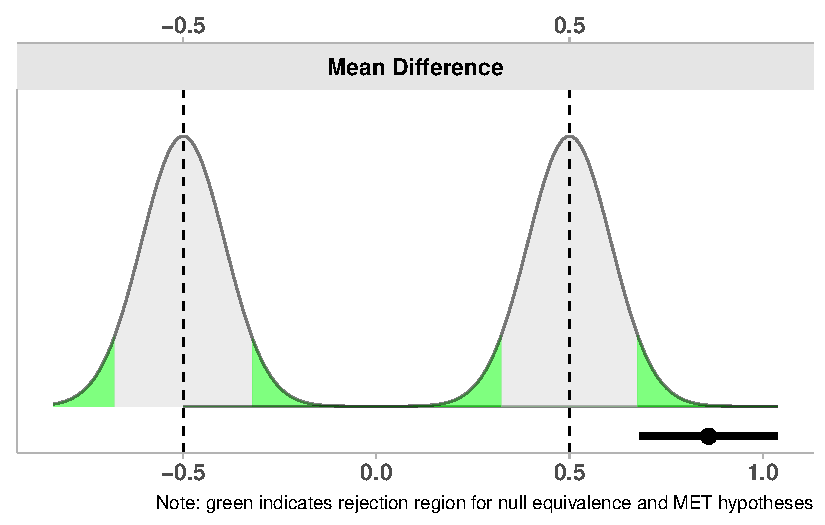
\includegraphics[width=1\textwidth,height=\textheight]{09-equivalencetest_files/figure-pdf/fig-tmet-1.pdf}

}

\caption{\label{fig-tmet}在进行最小效应量检验时,用于对-0.5和0.5进行两次单侧检验的\emph{t}分布下方绘制平均差及其置信区间}

\end{figure}

在这两条曲线下面,我们再次看到一条横线,它代表的置信区间从0.68至1.04,以及线上的点表示观察到的平均差0.86。整个置信区间远大于0.5的最小效应,因此我们不仅可以拒绝零效应的原假设,而且可以拒绝小于最小感兴趣效应的效应。因此,我们可以声称这种效应足够大,不仅在统计上具有显著性,而且在实践中也很有意义(只要我们很好地证明了我们最小感兴趣区)。因为我们进行了双侧最小效应量检验,如果置信区间完全在-0.5的另一侧,最小效应量检验也是显著的。

前面我们讨论了如何将传统的NHST和等价检验相结合,从而获得更多具有参考价值的结果。我们也可以将最小效应量检验和等价检验相结合。甚至可以说,无论何时,只要可以指定最小感兴趣效应大小,这种组合都是信息量最为丰富的检验。原则上,这是真实的。只要我们能够收集到足够的数据,当我们将最小效应量检验与等价检验相结合时,我们总是会得到一个信息丰富、直截了当的答案:要么我们可以拒绝所有太小而不关注的效应,要么我们可以拒绝所有足够大而值得关注的效应。正如我们将在下文关于区间假设的统计检验力分析一节中所看到的那样,每当真实效应量接近最小感兴趣区时,都需要收集大量的观测结果。如果真实效应量恰好与最小感兴趣区相同,则最小效应量检验和等价检验都不能被正确拒绝(任何显著的检验都将是Ⅰ型错误)。如果研究者能够收集充分的数据(从而使检验具有很高的统计检验力),并且相对确信真实效应量将大于或小于最小感兴趣效应,那么最小效应量检验和等价检验的组合可能很有吸引力,因为这样的假设检验可能会为研究问题提供信息丰富的答案。

\hypertarget{ux533aux95f4ux5047ux8bbeux68c0ux9a8cux7684ux68c0ux9a8cux529bux5206ux6790}{%
\section{区间假设检验的检验力分析}\label{ux533aux95f4ux5047ux8bbeux68c0ux9a8cux7684ux68c0ux9a8cux529bux5206ux6790}}

在设计研究时,一种明智的策略是始终同时计划效应存在与不存在两种情况。一些期刊要求对注册报告提供样本量的合理性证明,对于这些注册报告,其拒绝零假设的统计检验力很高,但研究也能够证明不存在效应。例如,同时对等价检验进行检验力分析。正如我们在\protect\hyperlink{errorcontrol}{误差控制}和\protect\hyperlink{likelihoods}{似然性}的章节中看到的那样,零效应是意料之中的,如果您在收完数据后才考虑观察到零效应的可能性,通常为时已晚。

区间假设的统计检验力取决于α水平、样本量、您决定检验的最小感兴趣效应以及真实效应大小。对于等价检验,通常假定真实效应大小为0来进行统计检验力分析,但有时可能并不现实。预期效应量越接近最小感兴趣区,需要达到所需统计检验力的样本量就越大。如果您有充分的理由预期一个小但非零的真实效应量,请不要试图假定真实效应量为0。统计检验力分析可能会表明您需要收集的样本量较小,但实际上您也更有可能得到不确定的结果。早期版本的
TOSTER 仅允许研究者在假设真实效应大小为 0
的情况下对等价检验进行统计检验力分析,但 Aaron Caldwell
的新统计检验力函数允许用户指定 \texttt{delta},即预期的效应量。

假设研究者希望等价检验达到 90\% 的统计检验力,等价范围为 -0.5 到
0.5,α水平为 0.05,并假设总体效应量为
0。此时可以进行等价检验的检验力分析,从而确定所需的样本量。

\begin{Shaded}
\begin{Highlighting}[]
\NormalTok{TOSTER}\SpecialCharTok{::}\FunctionTok{power\_t\_TOST}\NormalTok{(}\AttributeTok{power =} \FloatTok{0.9}\NormalTok{, }\AttributeTok{delta =} \DecValTok{0}\NormalTok{,}
                     \AttributeTok{alpha =} \FloatTok{0.05}\NormalTok{, }\AttributeTok{type =} \StringTok{"two.sample"}\NormalTok{,}
                     \AttributeTok{low\_eqbound =} \SpecialCharTok{{-}}\FloatTok{0.5}\NormalTok{, }\AttributeTok{high\_eqbound =} \FloatTok{0.5}\NormalTok{)}
\end{Highlighting}
\end{Shaded}

\begin{verbatim}

     Two-sample TOST power calculation 

          power = 0.9
           beta = 0.1
          alpha = 0.05
              n = 87.26261
          delta = 0
             sd = 1
         bounds = -0.5, 0.5

NOTE: n is number in *each* group
\end{verbatim}

我们看到,对于独立样本\emph{t}检验,所需的样本量为每个条件88名被试。现在,让我们将这个检验力分析与研究者预期真实效应为\emph{d}=
0.1的情况进行比较,而不是真实效应为0。为了能够可靠地拒绝大于0.5的效应,我们将需要更大的样本量,就像我们需要更大的样本量去测出\emph{d}
= 0.4的零假设检验,而不是\emph{d} = 0.5的零假设一样。

\begin{Shaded}
\begin{Highlighting}[]
\NormalTok{TOSTER}\SpecialCharTok{::}\FunctionTok{power\_t\_TOST}\NormalTok{(}\AttributeTok{power =} \FloatTok{0.9}\NormalTok{, }\AttributeTok{delta =} \FloatTok{0.1}\NormalTok{,}
                     \AttributeTok{alpha =} \FloatTok{0.05}\NormalTok{, }\AttributeTok{type =} \StringTok{"two.sample"}\NormalTok{,}
                     \AttributeTok{low\_eqbound =} \SpecialCharTok{{-}}\FloatTok{0.5}\NormalTok{, }\AttributeTok{high\_eqbound =} \FloatTok{0.5}\NormalTok{)}
\end{Highlighting}
\end{Shaded}

\begin{verbatim}

     Two-sample TOST power calculation 

          power = 0.9
           beta = 0.1
          alpha = 0.05
              n = 108.9187
          delta = 0.1
             sd = 1
         bounds = -0.5, 0.5

NOTE: n is number in *each* group
\end{verbatim}

我们可以看到,现在每个条件下的样本量都增加到了109人。如前所述,没有必要进行双侧等价检验。执行单侧等价检验是有可能的。复制研究就是适合进行这种方向性检验的一个例子。如果之前的一项研究观察到\emph{d}
= 0.48的效应,而你进行了一项重复研究,你可能会决定将任何小于\emph{d} =
0.2的效应视为复制失败,包括任何反方向的效应,如\emph{d} =
-0.3的效应。虽然大多数等价检验软件都要求你指定等价范围的上下限,但你可以模拟单侧检验,将你想忽略的方向上的等价范围设置为一个较低的值,这样针对该值的单侧检验将始终具有统计学意义义。这也可以用来执行最小效应量检验的检验力分析,其中一个界限是最小感兴趣效应,另一个界限则设置为预期效应量的另一侧的极端值。

在如下等价检验的统计检验力分析示例中,下限被设定为-5(应该设置得足够低,以至于进一步降低也不会有明显影响)。我们可以看到,TOSTER软件包中的新统计检验力函数考虑了方向性预测,与在零效应的原假设检验中的方向性预测一样,等价检验中的方向性预测更有效,且只需要70个观测值即可达到90\%的统计检验力。

\begin{Shaded}
\begin{Highlighting}[]
\CommentTok{\# New TOSTER power functions allows power for expected non{-}zero effect.}
\NormalTok{TOSTER}\SpecialCharTok{::}\FunctionTok{power\_t\_TOST}\NormalTok{(}\AttributeTok{power =} \FloatTok{0.9}\NormalTok{, }\AttributeTok{delta =} \DecValTok{0}\NormalTok{,}
                     \AttributeTok{alpha =} \FloatTok{0.05}\NormalTok{, }\AttributeTok{type =} \StringTok{"two.sample"}\NormalTok{,}
                     \AttributeTok{low\_eqbound =} \SpecialCharTok{{-}}\DecValTok{5}\NormalTok{, }\AttributeTok{high\_eqbound =} \FloatTok{0.5}\NormalTok{)}
\end{Highlighting}
\end{Shaded}

\begin{verbatim}

     Two-sample TOST power calculation 

          power = 0.9
           beta = 0.1
          alpha = 0.05
              n = 69.19784
          delta = 0
             sd = 1
         bounds = -5.0, 0.5

NOTE: n is number in *each* group
\end{verbatim}

统计软件为某些统计检验提供了统计检验力分析选项,但并非所有检验都有。就像零假设检验的统计检验力分析一样,可能有必要使用基于模拟的方法进行统计检验力分析。

\hypertarget{sec-ROPE}{%
\section{贝叶斯ROPE程序}\label{sec-ROPE}}

在贝叶斯估计中,一种论证缺乏有意义效应的方法是\textbf{实际等价区间}(ROPE)程序(Kruschke
(2013)),它''有点类似于频率学派的等价检验''(Kruschke \& Liddell
(2017))。在ROPE程序中,在 ROPE
程序中,与等价检验一样,也指定了等价范围,但使用的是基于后验分布的贝叶斯最高密度区间(如\protect\hyperlink{bayes}{贝叶斯统计}
章节所述)而不是置信区间。

如果Kruschke使用的先验分布完全一致,并且ROPE程序和等价检验使用相同的置信区间(例如90%),那么这两种检验将产生相同的结果。只是在如何解释数字上存在哲学差异。在R中可以使用\texttt{BEST}
软件包执行ROPE程序,该软件包默认使用''广义''的先验值,因此ROPE程序和等价检验的结果并不完全相同,但非常接近。甚至可以说这两种检验
``实际上是等价的''。下面的R代码生成了两个条件下的随机正态分布数据(均值为0,标准差为1),并执行了ROPE程序和TOST等价检验。

\begin{verbatim}
Waiting for parallel processing to complete...done.
\end{verbatim}

\begin{figure}

{\centering 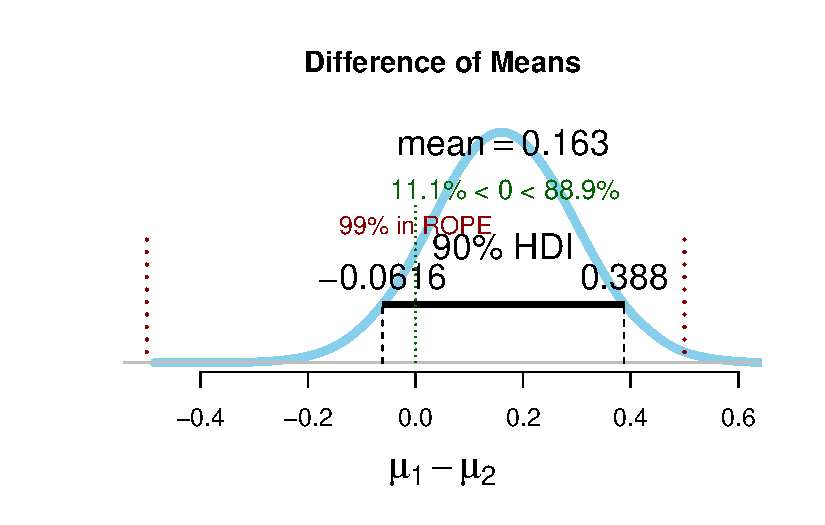
\includegraphics[width=1\textwidth,height=\textheight]{09-equivalencetest_files/figure-pdf/unnamed-chunk-6-1.pdf}

}

\end{figure}

\begin{figure}

{\centering 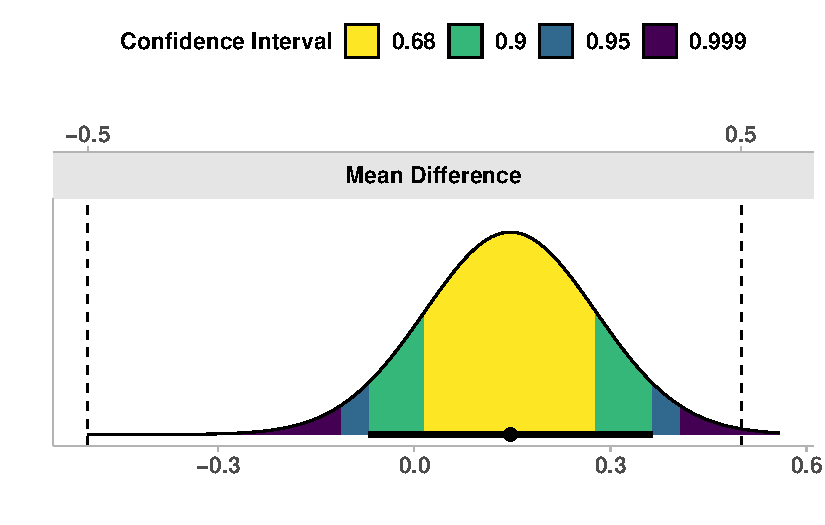
\includegraphics[width=1\textwidth,height=\textheight]{09-equivalencetest_files/figure-pdf/unnamed-chunk-6-2.pdf}

}

\end{figure}

90\%
HDI范围在-0.06到0.39之间,基于先验值和数据估计的平均值为0.164。HDI完全落在等价范围的上限和下限之间,因此比-0.5或0.5更极端的值被认为是不可信的。95\%
CI范围从-0.07到 0.36
,观察到的平均差异为0.15。我们看到,这些数字并不完全相同,因为在贝叶斯估计法中,观测值与先验值相结合,而平均值估计并不仅仅基于数据。但结果非常相似,在大多数情况下会得出相似的推论。BEST
R软件包还能让研究者执行基于模拟的统计检验力分析,这种分析需要很长时间,但是使用广义先验时,其结果与等价检验的统计检验力分析的样本量基本相同。ROPE相对于TOST的最大优势在于它允许您纳入先验信息。如果你有可靠的先验信息,ROPE可以使用此信息,这在你没有大量数据时尤其有用。如果你使用的是知情先验,建议进行敏感性分析,检查后验在先验发生合理变化时的稳健性。

\hypertarget{sec-whichinterval}{%
\section{应该使用哪个区间宽度?}\label{sec-whichinterval}}

因为 TOST 程序基于两个单侧检验,所以当在 5\% 的 alpha
水平下执行单侧检验时,将使用 90\%
的置信区间。因为针对上限的检验和针对下限的检验都需要具有统计显著性才能声明等价(正如在\protect\hyperlink{multiplecomparisons}{误差控制}
一章中所解释的那样,等价是多重检验的交-并集方法),所以不必因为进行了两次检验而修正结果。如果针对多重比较调整了
alpha 水平,或者如果 alpha 水平是合理的而不是依赖于默认的 5\%
水平(或两种条件都满足),则应使用相应的置信区间,即CI = 100 - (2 *
\(\alpha\))。因此,置信区间的宽度与alpha水平的选择直接相关,我们需要根据置信区间是否排除了所检验的效应来决定是否拒绝最小效应量。

当从贝叶斯角度出发使用最高密度区间时,比如ROPE程序,置信区间宽度的选择在逻辑上并不符合预期的错误率或任何其他原则。Kruschke(2014)写道:``我们应该如何定义'合理可信'?一种方法是说,任何在95\%
HDI内的点都是合理可信的。''McElreath
(2016)推荐使用67\%、89\%和97\%,他认为''没有什么理由,因为它们是质数便于记忆。''
这两种建议都缺乏坚实的依据。正如Gosset(笔名Student)观察到的(1904):

\begin{quote}
结果仅在它们与真相相差的程度足够小以至于在实验目的上可以忽略不计时才有价值。选定的机率应取决于以下两点:
1.实验允许的精度水平; 2.相关问题的重要性。
\end{quote}

有两种原则性的解决方案。首先,如果使用最高密度区间宽度来进行声明,这些声明将具有一定的错误率,且研究者需要通过计算频率学派的错误率来量化错误声明的风险。这将使ROPE成为贝叶斯/频率学派的折中程序,其后验分布计算能够对参数值的可能性进行贝叶斯解释,而基于
HDI
是否落在等价范围内做出的决策则具有一个受控制的错误率。请注意,当使用信息先验时,HDI与CI不匹配,则使用HDI的错误率只能通过模拟来推导。第二种解决方案是不进行任何声明,展示完整的后验分布,从而让读者自己得出结论。

\hypertarget{sec-sesoi}{%
\section{设置感兴趣的最小效应量}\label{sec-sesoi}}

要使用等价检验来验证我们的预测是否正确,就是要明确规定哪些观察值太小而无法用我们的理论进行预测。我们永远无法说效应完全为零,但我们可以研究观察到的效应是否太小而不具备理论或实际上的重要性。这需要我们指定\textbf{最小感兴趣区}(SESOI)。同样的概念有许多名称,比如最小重要差异或临床显著差异(King,
2011)。花些时间思考一下,对于你正在设计的下一项研究,最小效应量是多少才可以被认为是理论或实际上有意义的?确定你的最小感兴趣区可能很困难,并且最小感兴趣区是多少,你可能从来没想过在研究设计的一开始需要思考这个问题。然而,确定最小感兴趣区对于实践有重要的好处。首先,如果某个领域的研究者能够确定哪些效应太小而不重要,那么就可以非常直接地为有意义的效应确定研究所需的统计检验力。其次,指定最小感兴趣区的好处是可以你的研究具有可证伪性。你的预测被别人证伪对你个人来说可能感觉不太好,但对整个科学界来说却非常有用(Popper,2002)。毕竟,如果某种预测不会出错,那么预测正确怎么令人影响深刻的呢?

要开始思考哪些效应量是重要的,先问问自己,在预测方向上的\emph{任何}效应是否实际上支持备择假设?例如,Cohen's
\emph{d} 为 10
的效应量是否支持你的假设?在心理学中,理论很少会预测如此巨大的效应量。如果发现
d =
10,你很可能会检查是否有计算错误或研究中存在混淆变量。另一方面,\emph{d}
= 0.001
的效应量是否符合理论提出的机制?这样的效应量非常小,远低于个体能注意到的水平,因为它低于感知和认知限制下的\emph{最小可觉差}。因此,在大多数情况下,\emph{d}
= 0.001
会让研究者得出结论:``嗯,这实在是太小了,根本不符合我的理论预测,这么小的效果,几乎等同于没有效果。''然而,当我们做出方向性预测时,我们会说这种类型的效应全都是我们备择假说的一部分。尽管许多研究者会同意这种微小的影响太小而不重要,但如果我们有含零效应原假设的方向性预测,它们仍是支持我们备择假设的依据。此外,研究者很少有相应资源从统计上拒绝如此小的效应存在,因此声称这种效应仍支持理论预测会让该理论变得\emph{实际上不可证伪}:研究者可以简单地回应任何显示出非显著小效应的重复性研究(例如
\emph{d} = 0.05):``这并没有证伪我的预测,我想效应只是比 \emph{d} =
0.05
稍微小一些'',而无需承认预测已被证伪。这是有问题的,因为如果我们没有重复和证伪的过程,科学学科就存在变得不可证伪的风险(Ferguson
\& Heene,
2012)。因此,当你设计实验或有理论和理论预测时,只要有可能,请仔细考虑并清楚说明你的最小感兴趣区是多少。

\hypertarget{ux6839ux636eux7406ux8bbaux6765ux6307ux5b9asesoi}{%
\section{根据理论来指定SESOI}\label{ux6839ux636eux7406ux8bbaux6765ux6307ux5b9asesoi}}

一个理论预测最小感兴趣区的例子可以从Burriss等人(2015)的研究中找到,他们研究了女性在排卵周期的生育期是否会出现面部发红的现象。他们的假设认为,皮肤稍红意味着更有吸引力和身体更健康,向男性发出这种信号会产生进化优势。这一假设的前提是,男性可以用肉眼发现皮肤变红。Burriss等人收集了22名女性的数据,结果表明她们面部皮肤的红润度确实在生育期增加了。然而,这种增加的幅度不足以让男性用肉眼察觉,因此这一假设被证伪了。由于可以测量出皮肤发红程度的最小可觉差,因此可以建立一个理论上可行的
SESOI。理论上的最小感兴趣区可以从最小可觉差中推导出来,它提供了能够影响个体的效应量下限,或者基于计算模型,它可以提供模型中参数的下限,该参数仍能解释实证文献中的观察结果。

\hypertarget{ux951aux5b9aux6cd5ux8bbeux7f6e-sesoi}{%
\section{锚定法设置 SESOI}\label{ux951aux5b9aux6cd5ux8bbeux7f6e-sesoi}}

基于最小可觉差这一概念,心理学家通常会对足以被单个个体注意到的效应感兴趣。锚定法是估计个体层面上何为有意义变化的一种程序(Jaeschke
et al., 1989; King, 2011; Norman et al.,
2004)。该方法需要在两个时间点收集测量数据(例如,治疗前后的生活质量测量)。在第二个时间点,使用一个独立测量指标(锚)来确定患者与时间点
1
相比是没有变化,还是有所改善或恶化。通常,患者会被直接要求回答锚点问题,并指出与时间点
1 相比,他们在时间点 2 的主观感受是相同、更好还是更差。Button et al.
(2015) 使用锚定法估计出贝克抑郁量表的最小临床显著差异对应基线分数降低
17.5\%。

Anvari和Lakens(2021)
应用锚定法来研究广泛使用的积极和消极情绪量表(PANAS)所测量的最小感兴趣区。被试在相隔数天的两个时间点完成了含
20 个项目的 PANAS(使用李克特量表,从1 =``非常轻微或根本没有''到5
=``极其严重'')。他们还被要求指出自己的情绪是变化了一点、变化了很多还是完全没有变化。当人们表示他们的情绪''有一点''变化时,以
Likert
单位计算,积极情绪的平均变化是0.26分,消极情绪的平均变化是0.28分。因此,如果采取干预措施来改善人们的情感状态,并使个人主观上认为至少有了一点改善,那么可以将SESOI设置为PANAS量表上的0.3个单位。

\hypertarget{ux6839ux636eux6210ux672cux6548ux76caux5206ux6790ux786eux5b9asesoi}{%
\section{根据成本效益分析确定SESOI}\label{ux6839ux636eux6210ux672cux6548ux76caux5206ux6790ux786eux5b9asesoi}}

另一种证明最小感兴趣区的原则性方法是进行成本效益分析。研究表明,认知训练可能改善老年人的心智能力,从而使老年驾驶员受益(Ball
et al.,
2002)。基于这些研究结果,Viamonte、Ball和Kilgore(2006)进行了成本效益分析并得出结论:根据干预成本(247.50美元),75岁以上驾驶员发生事故的概率(\emph{p}
0.0710)和单次事故的成本(22,000美元),对所有75岁及以上驾驶员进行干预比不干预或仅在筛查测试后干预更有效。此外,敏感性分析表明,只要碰撞风险降低25\%,对所有驾驶者进行干预仍然是有益的。因此,可以将
75 岁以上老年人发生车祸的概率降低 25\% 设置为最小感兴趣区。

另一个例子,经济学家根据人们为降低死亡风险愿意支付的费用,将统计生命的价值定为150万到250万美元之间(2000年,在西方国家,参见
Mrozek \& Taylor
(2002))在此基础上,Abelson(2003)计算出人们为预防急性健康问题(如眼睛不适)而支付的意愿约为每天
40-50
美元。研究者可能正在研究一种心理干预措施,可以减少人们接触眼周面部皮肤的次数,从而减少细菌引起的眼部刺激。
如果实施干预每年花费 20
美元,那么应该将人群产生眼部刺激的平均天数减少至少 0.5
天,这样的干预措施才是值得的。成本效益分析也可以基于对研究极小效应所需资源与这一知识对科学界价值之间的权衡。

\hypertarget{ux4f7fux7528ux5c0fux578bux671bux8fdcux955cux6cd5ux786eux5b9a-sesoi}{%
\section{使用小型望远镜法确定
SESOI}\label{ux4f7fux7528ux5c0fux578bux671bux8fdcux955cux6cd5ux786eux5b9a-sesoi}}

理想的情况是,研究者在做出经验性声明时,总是明确指出哪些观察结果能够证伪其声明。
遗憾的是,这种做法尚未普及。当研究者对先前研究进行极其接近的重复性研究时,这尤其成问题。因为永远无法证明一个效应完全为零,而原作者也很少说明哪种效应量范围能证伪他们的假设,所以事实证明复制研究的结果很难解释(S.
F. Anderson \& Maxwell, 2016)。新数据何时与原始发现相矛盾?

考虑一项研究,你想在其中检验群体智慧这一概念。你请 20
个人估算一个罐子里的硬币数量,期望平均值非常接近真实值。
研究问题是平均来说,这些人能否正确地猜出硬币数量是 500 枚。观察到 20
人的平均猜测值为 550,标准差为
100。观察到的与真实值的差异具有统计学意义,\emph{t} (19)=2.37,\emph{p}
= 0.0375,Cohen's \emph{d} 为 0.5。 群体平均值真的会相差如此之远吗?
群体智慧不存在吗?
你使用的硬币是否有什么特别之处,导致猜测硬币数量特别困难?
还是只是侥幸?你开始对此进行近似重复研究。

你希望你的研究不论是否存在效应都能提供有意义的信息。这意味着您需要设计一项复制研究,无论备择假设是否为真(群体无法准确猜测硬币的真正数量)或零假设是否为真(人们会猜出500枚硬币,原始的研究是巧合),都能让您得出有参考价值的结论。但是,由于最初的研究者并没有指定一个最小的目标效应量,那么什么时候复制研究才能让你得出新数据与原始研究相矛盾的结论呢?有些人可能会认为,观察到平均数正好是
500 非常有说服力,但由于随机变异,你(几乎)永远也找不到平均数正好是 500
的结果。不显著的结果不能解释为没有影响,因为你的研究可能样本量太小,无法检测到有意义的影响,且结果可能是第二类错误。那么,我们如何才能确定有意义的效应量呢?怎样才能设计出能够证伪先前发现的研究?

Uri
Simonsohn(2015)将小效应定义为''能够给原始研究提供33%的统计检验力的研究''。换句话说,如果效应存在,该效应量使得原始研究有1/3的可能观察到统计显著性。如果原始研究有33\%的统计检验力,且效应真实存在的话,那么在该研究中观察到显著效果的概率就太低了,无法可靠地区分信号和噪音(或有真实效果和没有真实效果的情况)。
Simonsohn(2015,第561页)称之为\textbf{小型望远镜法},并写道:``想象一位天文学家声称用望远镜发现了一颗新行星。另一位天文学家试图用更大的望远镜复制这一发现,却一无所获。虽然这并不能证明这颗行星不存在,但它确实与最初的发现相矛盾,因为用较小的望远镜可以观测到的行星,用较大的望远镜也应该可以观测到。''

虽然这种设定最小感兴趣区(SESOI)的方法很随意(为什么不是30\%或35\%?),但在实际应用中已经足够了(你也可以自由选择你认为过低的统计检验力水平)。这样定义SESOI的好处是,如果你知道原始研究的样本量,就可以计算出该研究33\%统计检验力时探测到的效应量。因此,你始终可以使用这种方法来设置最小感兴趣区。如果你未能找到原始研究33\%统计检验力所探测到的效应量有关证据,这并不意味着不存在真正的效应,甚至也不意味着效应太小而没有任何理论或实际意义。但是,使用小型望远镜法是很好的第一步,因为它可以让人们开始讨论哪些效应是有意义的,并让想要复制研究的研究者明确何时可以认为原来的声明已被证伪。

使用小型望远镜法时,SESOI仅基于原始研究的样本量。最小感兴趣区仅针对同方向的效应。
所有小于此效应的(包括反方向的大效应)都被解释为未能重复原始结果。我们可以看到,小型望远镜法是一种\textbf{单侧等价检验},其中只规定了上限,最小感兴趣区是根据原始研究的样本量确定的。该检验我们是否可以拒绝与原始研究有33%统计检验力检测到的效应一样大或更大的效应。它是一个简单的单侧检验,不是针对0,而是针对SESOI。该检验考察的是,我们是否能拒绝与原始研究33\%统计检验力所探测到的一样大或更大的效应。这是一个简单的单侧检验,不是针对
0,而是针对 SESOI。

例如,在上述研究中,有 20 位竞猜者试图估计硬币的数量。结果采用双侧单样本
\emph{t} 检验进行分析,α水平为0.05。为了确定本研究具有 33\%
统计检验力的效应量,我们可以进行敏感性分析。 在敏感性分析中,我们根据
alpha、样本量和所需的统计检验力计算所需的效应量。 请注意,Simonsohn
在他的统计检验力分析中使用了双侧检验,我们在此也将沿用这一方法----如果原始研究报告了预定的方向性预测,则统计检验力分析应基于单侧检验。
在这种情况下,alpha 水平为 0.05,总样本量为 20,所需统计检验力为
33\%。我们计算了能够产生 33\% 统计检验力的效应量,发现它是 0.358 的
Cohen's \emph{d}。 这意味着我们可以将重复研究最小感兴趣区设置为 \emph{d}
= 0.358。 如果我们能拒绝等于或大于 \emph{d} = 0.358
的效应,我们就可以得出结论,该效应小于原始研究33\%统计检验力所能探测到的效应。
下面的屏幕截图说明了 G*Power 中的正确设置,R 中的代码如下:

\begin{Shaded}
\begin{Highlighting}[]
\FunctionTok{library}\NormalTok{(}\StringTok{"pwr"}\NormalTok{)}

\NormalTok{pwr}\SpecialCharTok{::}\FunctionTok{pwr.t.test}\NormalTok{(}
  \AttributeTok{n =} \DecValTok{20}\NormalTok{, }
  \AttributeTok{sig.level =} \FloatTok{0.05}\NormalTok{, }
  \AttributeTok{power =} \FloatTok{0.33}\NormalTok{, }
  \AttributeTok{type =} \StringTok{"one.sample"}\NormalTok{,}
  \AttributeTok{alternative =} \StringTok{"two.sided"}
\NormalTok{)}
\end{Highlighting}
\end{Shaded}

\begin{verbatim}

     One-sample t test power calculation 

              n = 20
              d = 0.3577466
      sig.level = 0.05
          power = 0.33
    alternative = two.sided
\end{verbatim}

\begin{figure}

{\centering 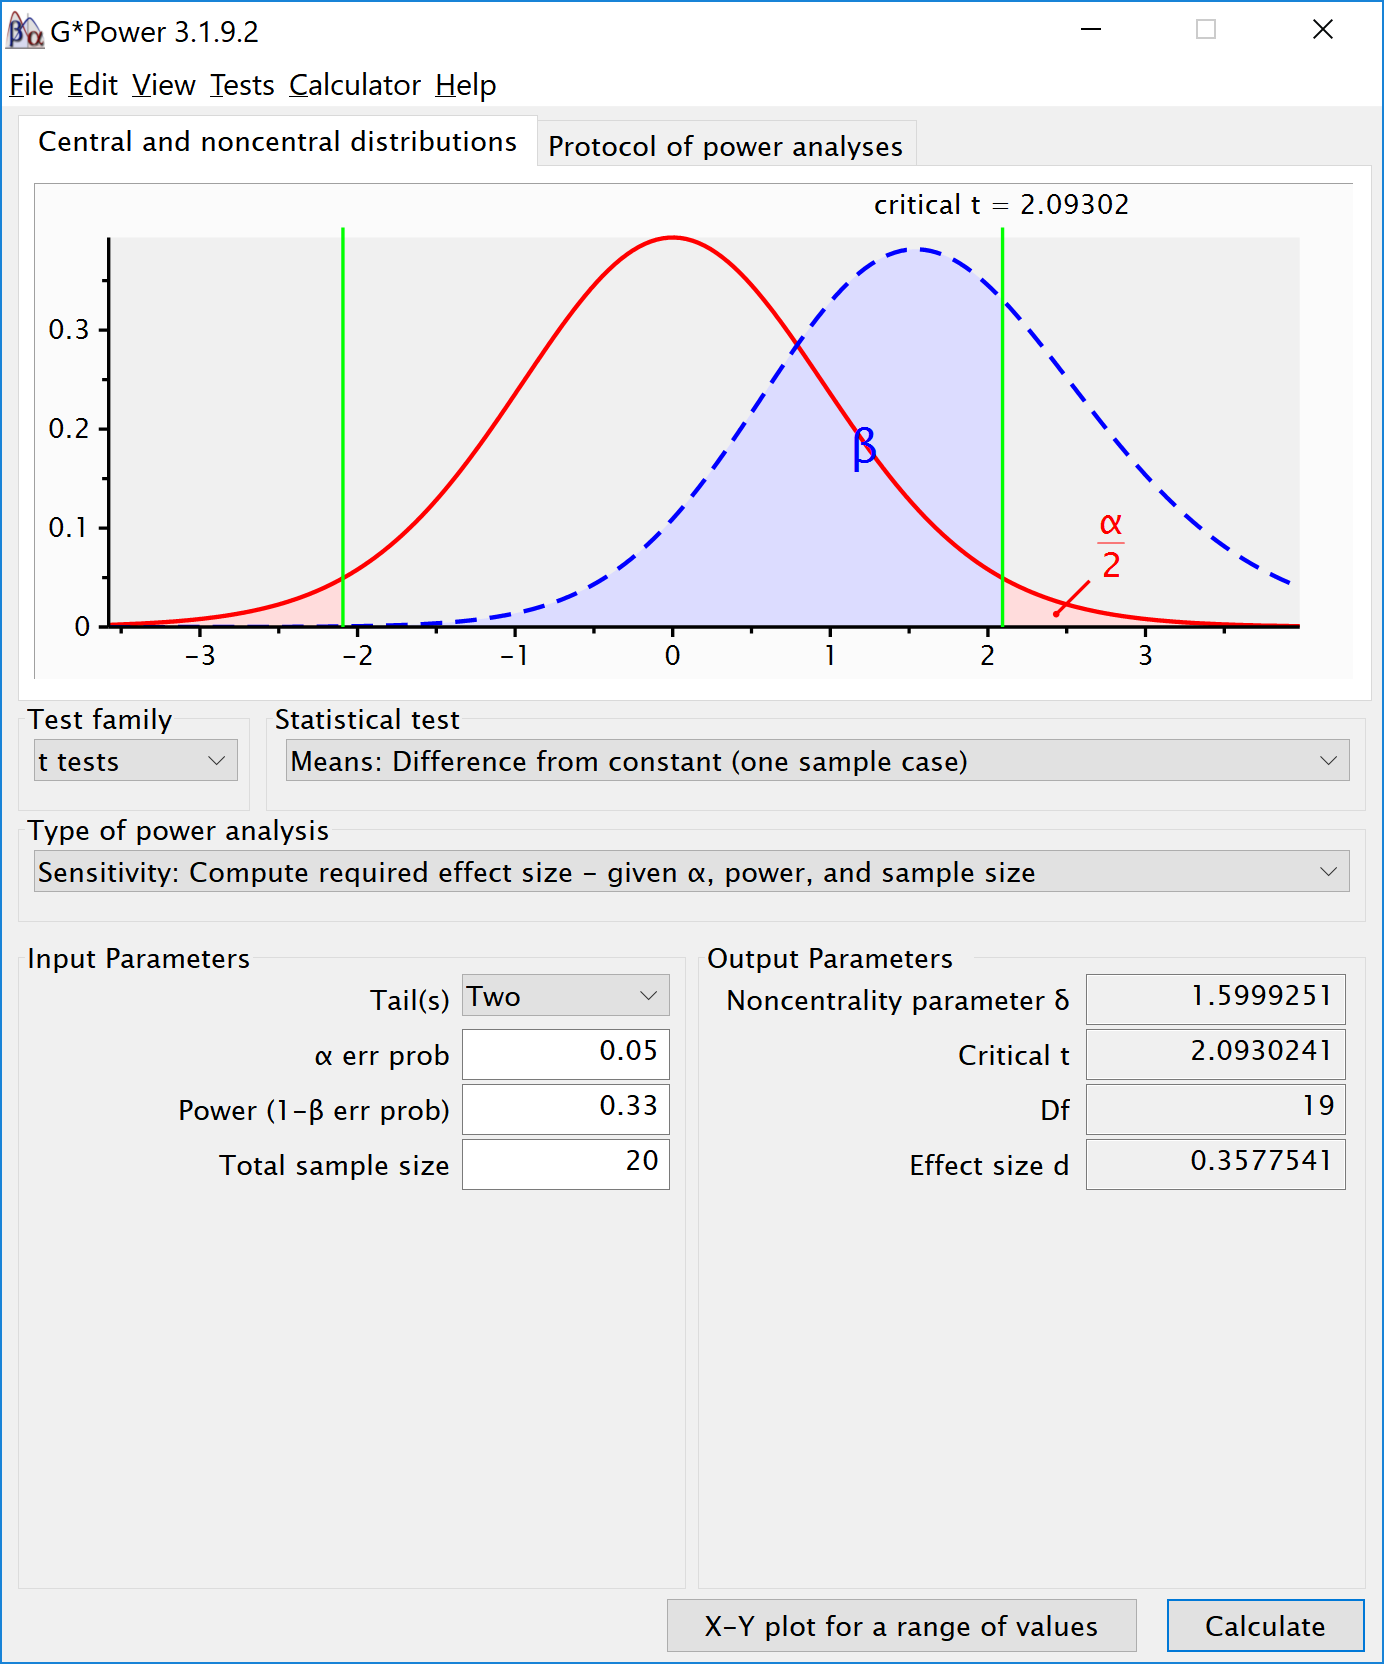
\includegraphics[width=1\textwidth,height=\textheight]{images/0deabffd850f7b63c16e41e0af9ae0b6.png}

}

\caption{\label{fig-smalltelpower}G*Power中演示敏感性检验力分析的截图,用于计算原始研究能够检测到33\%检验力的效应量。}

\end{figure}

基于原始研究33\%统计检验力所探测到的效应量来确定最小感兴趣区还有一个好处:假设真实的效应量为0,你基于小望远镜方法进行统计检验,看看数据在统计学上是否小于
SESOI(这也被称作劣势检验)。如果将样本量增加 2.5
倍,假定真实效应量正好为 0(例如,\emph{d} =
0),那么这种单侧等价检验的统计检验力将达到约 80\%。
进行重复研究的人可以遵循小型望远镜法的建议,并且可以很轻松地确定最小感兴趣区和设计有意义的重复研究所需的样本量,假定真实效应量为
0(但请参阅上文关于先验统计检验力分析的部分,在这里你想检验等价性,但并不期望真实效应大小为
0)。

下图来自 Simonsohn(2015),通过现实生活中的真实例子说明了小型望远镜法。
Zhong 和 Liljenquist(2006)的原始研究样本量很小,每个条件下只有 30
名参与者,观察到的效应大小为 \emph{d} =
0.53,这与零几乎没有统计学差异。考虑到每个条件下的样本量为 30
人,该研究有 33\% 的统计检验力探测到大于 \emph{d} = 0.401
的效应。这种''小效应''由绿色虚线表示。 在 R
中,最小感兴趣区是通过以下方法计算的:

\begin{Shaded}
\begin{Highlighting}[]
\NormalTok{pwr}\SpecialCharTok{::}\FunctionTok{pwr.t.test}\NormalTok{(}
  \AttributeTok{n =} \DecValTok{30}\NormalTok{, }
  \AttributeTok{sig.level =} \FloatTok{0.05}\NormalTok{, }
  \AttributeTok{power =} \DecValTok{1}\SpecialCharTok{/}\DecValTok{3}\NormalTok{, }
  \AttributeTok{type =} \StringTok{"two.sample"}\NormalTok{,}
  \AttributeTok{alternative =} \StringTok{"two.sided"}
\NormalTok{)}
\end{Highlighting}
\end{Shaded}

\begin{verbatim}

     Two-sample t test power calculation 

              n = 30
              d = 0.401303
      sig.level = 0.05
          power = 0.3333333
    alternative = two.sided

NOTE: n is number in *each* group
\end{verbatim}

请注意,33\%的统计检验力是一个四舍五入值,计算时使用了1/3(或0.3333333
\ldots)。

\begin{figure}

{\centering 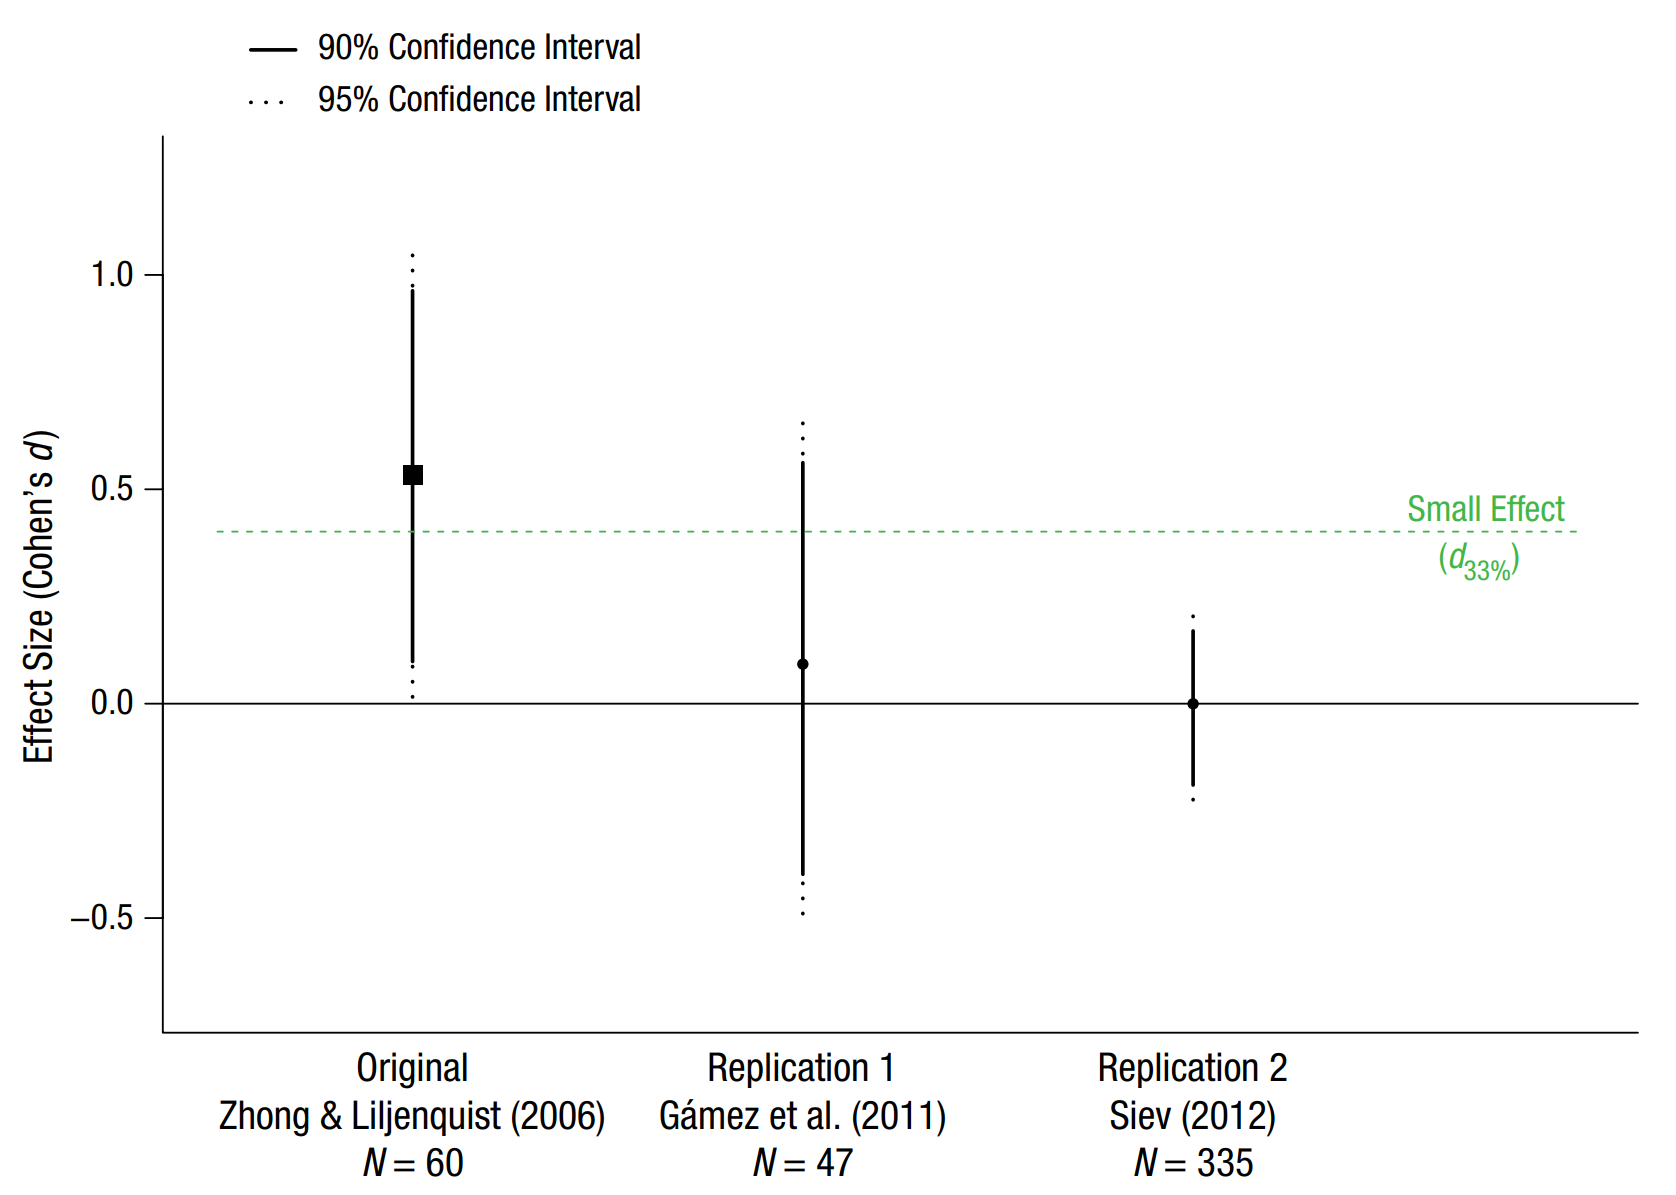
\includegraphics[width=1\textwidth,height=\textheight]{images/a4aa20a6e2dadfbaa82bc614d40693c7.png}

}

\caption{\label{fig-simonsohnexample}Simonsohn (2015)
在一项原始研究和两项重复研究中使用的示例。}

\end{figure}

我们可以看到,Gámez及其同事进行的第一次重复研究也具有相对较小的样本量(N
= 47,相对于原始研究中的N =
60),并且不是为了通过小型望远镜法产生有意义的结果而设计的。置信区间非常宽,包括零效应(\emph{d}
= 0)和最小感兴趣区(\emph{d} =
0.401)。因此,这项研究没有得出结论。我们不能拒绝零效应,但也不能拒绝0.401或更大的效应量,因为这仍然符合原始结果。第二次重复研究的样本量要大得多,它告诉我们,我们无法拒绝零效应,但我们可以拒绝最小感兴趣区,这表明该效应小于根据小望远镜方法得出的值得关注的效应量。

虽然\emph{小望远镜法}的建议易于使用,但应注意不要将任何统计程序变成启发式程序。
在我们上面关于20名被试的例子中,Cohen's
\emph{d}为0.358被用作最小感兴趣区,收集的样本量为50个(是原来20个的2.5倍),但如果有人愿意努力进行重复性研究,收集更大的样本量就会相对容易。另一种情况是,如果原始研究的规模非常大,那么它就会有很高的统计检验力来探测出实际上可能并不显著的效应,且我们也不希望在重复研究中收集2.5倍于原始研究的观测值。
事实上,正如Simonsohn所写:``我们是否需要原始样本量的2.5倍取决于我们希望回答的问题。如果我们想检验效应量是否小于33%,那么,无论原始样本量如何,我们都需要大约2.5倍的原始样本量。但是,当样本非常大时,这可能就不是我们感兴趣的问题了。''请始终考虑你想要提出的问题,并设计研究,为你感兴趣的问题提供有参考价值的答案。不要盲目遵循2.5倍n的启发式方法,并且始终思考建议的程序是否适合你的情况。

\hypertarget{ux628aux6700ux5c0fux611fux5174ux8da3ux533aux8bbeux7f6eux4e3aux7edfux8ba1ux5b66ux53efux63a2ux6d4bux5230ux7684ux6700ux5c0fux6548ux5e94}{%
\section{把最小感兴趣区设置为统计学可探测到的最小效应}\label{ux628aux6700ux5c0fux611fux5174ux8da3ux533aux8bbeux7f6eux4e3aux7edfux8ba1ux5b66ux53efux63a2ux6d4bux5230ux7684ux6700ux5c0fux6548ux5e94}}

在给定样本量和 α 水平的情况下,每个检验都有一个
\protect\hyperlink{minimaldetectable}{统计学可探测到的最小效应}。例如,如果测试中每组有
86 名参与者,且 α 水平为 5\%,只有 \emph{t} ≥ 1.974 的 \emph{t}
检验才具有统计显著性。 换句话说,\emph{t} = 1.974 是\textbf{临界
\emph{t} 值}。 给定样本量和 α 水平,可以将临界 \emph{t}
值转换为\textbf{临界 \emph{d} 值}。如图 Figure~\ref{fig-distpowerplot1}
所示,每组 n = 50,α 水平为 5\%,临界 \emph{d} 值为
0.4。这意味着只有大于 0.4 的效应才会产生 \emph{p} \textless{} α。 临界
\emph{d} 值受每组样本量和 α 水平的影响,但与真实效应量无关。

\begin{figure}

{\centering 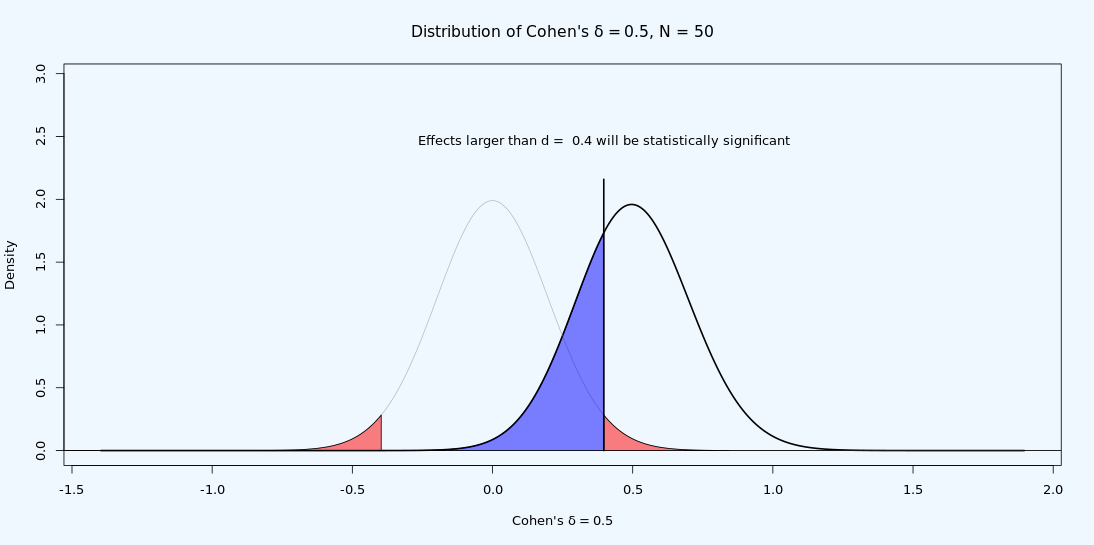
\includegraphics[width=1\textwidth,height=\textheight]{images/dpplot50.png}

}

\caption{\label{fig-distpowerplot1}具有一类和二类错误的零分布和备择分布表明,在每个条件为
n = 50时,最小的效应量将具有统计显著性。}

\end{figure}

如果真实效应量\emph{小于}临界效应量,则有可能观察到统计上显著的检验结果。由于随机变异,有可能在\emph{样本}中观察到比群体中真实值更大的值。这就是为什么在零假设显著性检验中,统计检验力永远不为零的原因。正如图
Figure~\ref{fig-distpowerplot2}
所示,即使真实效应量小于临界值(例如,真实效应量为0.2),我们也可以从分布图中看到,当\emph{真实群体效应量}为
\emph{d} =
0.2,我们可以预期一些\emph{观察到的效应量}大于0.4------如果我们计算这个检验的统计检验力,结果表明从长远来看,我们可以预期\emph{观察到的效应量}中有
16.77\% 会大于 0.4。
这并不算多,但也是有意义的。这也是为什么发表偏倚加上研究统计检验力不足是很有问题的:如果文献中观察到显著结果的效应量只来自统计检验力不足的研究,这将导致\emph{对真实效应量的大幅高估}。

\begin{figure}

{\centering 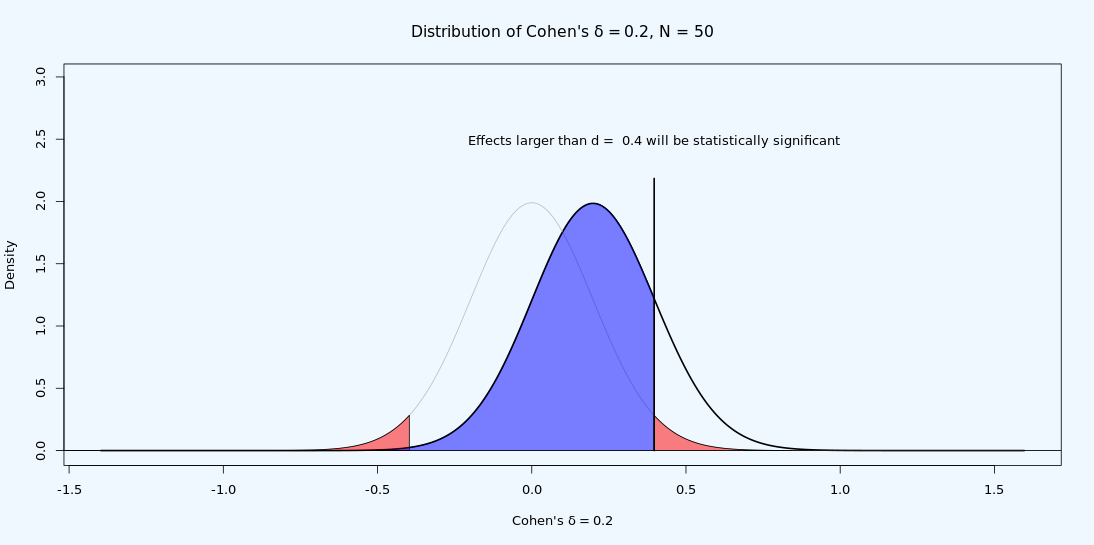
\includegraphics[width=1\textwidth,height=\textheight]{images/dpplot502.png}

}

\caption{\label{fig-distpowerplot2}具有一类和二类错误的零分布和备择分布表明,,在每个条件为
n = 50时,最小效应量将具有统计显著性。}

\end{figure}

我们可以使用统计学上可探测到的最小效应来设置重复研究的SESOI。如果你试图重复一项研究,选择最小感兴趣区(SESOI)时的一个合理选项是使用你所重复的研究中可能具有统计显著性的最小观察效应量。换句话说,你可以决定在原始研究中无法产生小于α的\emph{p}值的效应,它们在复制研究中将被认为是没有意义的。这里的假设是,原作者希望观察到显著效应,因此对观察到无法产生显著结果的效应量不感兴趣。原作者很可能没有考虑到他们的研究在统计学上有足够的统计检验力探测到哪些效应量,或者他们对更小的效应感兴趣,但承受着认为观察到的大效应只是来源于随机变异所带来的风险。即便如此,在没有指定SESOI的早期研究的基础上,一个合理的出发点可能是将SESOI设定为在原始研究中观察到的\textbf{可能具有统计学意义}的最小效应量。并非所有研究者都会同意这一点(例如,原始作者可能会说他们实际上也关心\emph{d}

0.001的效应)。然而,当我们试图改变这一领域当前的状况时,即没有人明确指出什么能证伪他们的假说,或者他们的最小感兴趣区是多少,这种方法不失为一种起步方式。在实践中,如\protect\hyperlink{posthoc}{事后检验力}部分所解释的,对于观察到的效应量而言,
由于\emph{p} = 0.05 与观察效应量 50\% 统计检验力之间的关系,这种对 SESOI
的合理性证明将意味着 SESOI 被设置为原始研究在独立\emph{t}检验中有 50\%
的统计检验力来探测的效应量。这种方法在某些方面与 Simonsohn (2015)
提出的小型望远镜法相似,只是它将导致更大的 SESOI。

为重复研究设置最小感兴趣区有点像一场网球比赛。原作者发球并将球击过球网,说''看,有情况''。将SESOI设置为在原始研究中可能具有显著性的效应量的方法是回球,它允许你在通过一项精心设计、统计检验力较高的重复研究后说''你的原始研究中似乎没有足够大的显著效应'',从而拒绝SESOI。这并不是比赛的结束------原作者可以尝试还击,就他们的理论所预测的效应做出更具体的陈述,并证明存在这种较小的效应量。但球又回到了他们的手中,如果他们想继续声称存在效应,就必须用新的数据来支持他们的说法。

除了重复研究之外,所收集的数据量也限制了人们所能做出的推论。根据研究领域通常使用的样本量,也可以计算出统计学上可探测到的最小效应。例如,假设一个研究领域中的假说几乎总是通过执行单样本
\emph{t} 检验来验证,并且收集的样本量始终小于 100个观测值。对 100
个观测值进行单样本 \emph{t} 检验,使用 0.05 的 α(双侧),有 80\%
的统计检验力来探测到一个 \emph{d} = 0.28
的效应(可以通过灵敏度检验力分析计算得出)。在一项新的研究中,我们可以可靠地拒绝比
\emph{d} = 0.28 更极端的效应的存在,这一结论表明,在此类研究中,100
个样本量可能不足以探测出效应。 拒绝比 \emph{d} = 0.28
更极端效应的存在并不能检验理论预测,但它通过回答一个\textbf{资源问题}对文献做出了贡献。它表明,今后在这一研究方向上的研究需要改变研究设计,大幅增加样本量。基于这种方法设置最小感兴趣区并不能回答任何理论问题(毕竟,SESOI
不基于任何理论预测)。但是,如果告知同行,在某一领域通常收集的样本量下,效应还不够大,因此无法对其进行可靠的研究,这是对文献的有益贡献。这并不意味着该效应本身没有意义,同时某一领域可能会决定,是时候通过协调研究路线,共同研究该研究问题,并收集足够的数据,来可靠地研究是否存在较小的效应。

\hypertarget{ux81eaux6211ux6d4bux9a8c}{%
\section{自我测验}\label{ux81eaux6211ux6d4bux9a8c}}

\hypertarget{ux5173ux4e8eux7b49ux6548ux68c0ux9a8cux7684ux95eeux9898}{%
\subsection{关于等效检验的问题}\label{ux5173ux4e8eux7b49ux6548ux68c0ux9a8cux7684ux95eeux9898}}

\textbf{问题1}:当均值差异的90\%置信区间落入等效范围-0.4到0.4之间时,我们可以拒绝感兴趣的最小效应量。根据你对于置信区间的了解,当等效范围改变为变化为-0.3到0.3时,什么情况下等效检验才能显著(假定估计效应量和标准差不变)
? A) 更大的效应量。 B) 更低的α水平。 C) 更大的样本量。 D)
更低的统计检验力。

\textbf{问题2}:为什么在等效检验统计显著时,得出没有效应的结论是错误的?

\begin{enumerate}
\def\labelenumi{\Alph{enumi})}
\tightlist
\item
  等效检验只针对数据,而非效应的存在与否。
\item
  等效检验可能伴随着一类错误,因此,我们应该认为不存在效应,或者存在一类错误。
\item
  等效检验会拒绝与最小感兴趣效应同样大或者更大的数值,所以不能拒绝存在一个小的非零效应的可能性。
\item
  当等价检验不显著而非显著时,我们才可以得出效应不存在的结论。
\end{enumerate}

\textbf{问题3}:研究者想知道使用电子书的学生是否与使用纸质书的学生得表现一样好。如果一样好,他们就会建议教师允许学生自由使用媒介;但如果这两者有差异,他们则会推荐使用导致更好表现的那种媒介。他们随机分配学生使用电子书或者教科书,比较他们在考试中的成绩
课程(从最差的1分到最好的10分)。他们发现两组学生的表现相似,对于纸质教科书条件均值为
7.35,标准差为1.15,样本量为50,电子书均值为7.13,标准差为1.21,样本量为50)。假设我们认为任何大于或大于半个绩点(0.5)的影响都是值得的,但任何差异小于0.5,因为太小而无关紧要,alpha水平被设置为0.05。作者会得出什么结论?将下面的代码复制到R中,用正确的数字替换所有的0。输入?tsum\_TOST以获取该函数的帮助。

\begin{Shaded}
\begin{Highlighting}[]
\NormalTok{TOSTER}\SpecialCharTok{::}\FunctionTok{tsum\_TOST}\NormalTok{(}
  \AttributeTok{m1 =} \FloatTok{0.00}\NormalTok{,}
  \AttributeTok{sd1 =} \FloatTok{0.00}\NormalTok{,}
  \AttributeTok{n1 =} \DecValTok{0}\NormalTok{,}
  \AttributeTok{m2 =} \FloatTok{0.00}\NormalTok{,}
  \AttributeTok{sd2 =} \FloatTok{0.00}\NormalTok{,}
  \AttributeTok{n2 =} \DecValTok{0}\NormalTok{,}
  \AttributeTok{low\_eqbound =} \SpecialCharTok{{-}}\FloatTok{0.0}\NormalTok{,}
  \AttributeTok{high\_eqbound =} \FloatTok{0.0}\NormalTok{,}
  \AttributeTok{eqbound\_type =} \StringTok{"raw"}\NormalTok{,}
  \AttributeTok{alpha =} \FloatTok{0.05}
\NormalTok{)}
\end{Highlighting}
\end{Shaded}

\begin{enumerate}
\def\labelenumi{\Alph{enumi})}
\tightlist
\item
  我们可以\textbf{拒绝}效应值为零,也可以\textbf{拒绝}效应值大于或大于最小效应值的存在。
\item
  我们不能\textbf{拒绝}效应值为零,我们可以\textbf{拒绝}效应值大于或大于最小效应值的存在。
\item
  我们可以\textbf{拒绝}效应值为零,也可以\textbf{不拒绝}效应值大于或大于最小效应值的存在。
\item
  我们不能\textbf{拒绝}效应值为零,也不能\textbf{拒绝}效应值大于或大于最小效应值的存在。
\end{enumerate}

\textbf{问题4}:如果我们将问题3中的样本量增加到每个条件下150名参与者,并且假设观察到的平均值和标准差完全相同,我们会得出什么结论?

\begin{enumerate}
\def\labelenumi{\Alph{enumi})}
\tightlist
\item
  我们可以\textbf{拒绝}效应值为零,也可以\textbf{拒绝}效应值大于或大于最小效应值的存在。
\item
  我们不能\textbf{拒绝}效应值为零,我们可以\textbf{拒绝}效应值大于或大于最小效应值的存在。
\item
  我们可以\textbf{拒绝}效应值为零,也可以\textbf{不拒绝}效应值大于或大于最小效应值的存在。
\item
  我们不能\textbf{拒绝}效应值为零,也不能\textbf{拒绝}效应值大于或大于最小效应值的存在。
\end{enumerate}

\textbf{问题5}:如果我们将问题3中的样本量增加到每个条件下500名参与者,并且假设观察到的平均值和标准差完全相同,我们会得出什么结论?
A)
我们可以\textbf{拒绝}效应值为零,也可以\textbf{拒绝}效应值大于或大于最小效应值的存在。
B)
我们不能\textbf{拒绝}效应值为零,我们可以\textbf{拒绝}效应值大于或大于最小效应值的存在。
C)
我们可以\textbf{拒绝}效应值为零,也可以\textbf{不拒绝}效应值大于或大于最小效应值的存在。
D)
我们不能\textbf{拒绝}效应值为零,也不能\textbf{拒绝}效应值大于或大于最小效应值的存在。

有时检验的结果是\textbf{不确定的},如零假设检验和等效检验在统计上不显著。在这种情况下,唯一的解决方案是收集额外的数据。有时,零假设检验和等效检验在统计上都是显著的,在这种情况下,效果\textbf{在统计上不同于零,但实际上不显著}(基于SESOI的证明)。

\textbf{问题6}:我们可能想知道问题3中检验的统计检验力是多少,假设两组之间没有真正的差异(因此真实效应大小为0)。使用R包TOSTER中新改进的'power\_t\_TOST'函数,我们可以使用灵敏度功效分析(即输入每组50个样本量,假设真实效应大小为0,等效边界和alpha水平)计算统计检验力。请注意,由于等效边界是在问题3的原始尺度上指定的,因此我们还需要指定总体中真实标准偏差的估计值。假设真实标准差是1.2。把答案四舍五入到小数点后两位。输入?power\_t\_TOST
'获取函数的帮助。问题3的统计检验力是多少?

\begin{Shaded}
\begin{Highlighting}[]
\NormalTok{TOSTER}\SpecialCharTok{::}\FunctionTok{power\_t\_TOST}\NormalTok{(}
  \AttributeTok{n =} \DecValTok{15}\NormalTok{,}
  \AttributeTok{delta =} \FloatTok{0.0}\NormalTok{,}
  \AttributeTok{sd =} \FloatTok{1.2}\NormalTok{,}
  \AttributeTok{low\_eqbound =} \SpecialCharTok{{-}}\FloatTok{0.5}\NormalTok{,}
  \AttributeTok{high\_eqbound =} \FloatTok{0.5}\NormalTok{,}
  \AttributeTok{alpha =} \FloatTok{0.05}\NormalTok{,}
  \AttributeTok{type =} \StringTok{"two.sample"}
\NormalTok{)}
\end{Highlighting}
\end{Shaded}

\begin{Shaded}
\begin{Highlighting}[]
\NormalTok{TOSTER}\SpecialCharTok{::}\FunctionTok{power\_t\_TOST}\NormalTok{(}
  \AttributeTok{n =} \DecValTok{00}\NormalTok{,}
  \AttributeTok{delta =} \FloatTok{0.0}\NormalTok{,}
  \AttributeTok{sd =} \FloatTok{0.0}\NormalTok{,}
  \AttributeTok{low\_eqbound =} \SpecialCharTok{{-}}\FloatTok{0.0}\NormalTok{,}
  \AttributeTok{high\_eqbound =} \FloatTok{0.0}\NormalTok{,}
  \AttributeTok{alpha =} \FloatTok{0.05}\NormalTok{,}
  \AttributeTok{type =} \StringTok{"two.sample"}
\NormalTok{)}
\end{Highlighting}
\end{Shaded}

\begin{enumerate}
\def\labelenumi{\Alph{enumi})}
\tightlist
\item
  0.00
\item
  0.05
\item
  0.33
\item
  0.40
\end{enumerate}

\textbf{问题7}:假设在问题3每组只有15名参与者而不是50名。在这个较小的样本量下(其他条件如问题6中所示),检验的统计检验力是多少?答案四舍五入到两位小数。

\begin{enumerate}
\def\labelenumi{\Alph{enumi})}
\tightlist
\item
  0.00
\item
  0.05
\item
  0.33
\item
  0.40
\end{enumerate}

\textbf{问题8}:你可能还记得关于零假设显著性检验的统计检验力的讨论,统计检验力从不小于5\%(如果真实效应大小为0,统计检验力在形式上未定义,但我们将观察到至少5\%的一类错误,并且在引入真实效应时统计检验力增加)。在双尾等效检验中,统计检验力可以低于α水平。为什么?

\begin{enumerate}
\def\labelenumi{\Alph{enumi})}
\tightlist
\item
  因为在等效检验中,一类错误率没有限定在5\%。
\item
  因为在等效检验中,原假设和备择假设是相反的,因此二类错误率没有下界(就像零假设检验中的一类错误率没有下界一样)。
\item
  由于置信区间需要落在等效区间的下界和上界之间,并且样本量较小,因此该概率可以接近于1(因为置信区间非常宽)。
\item
  因为等效检验是基于置信区间,而不是基于\textbf{p}值,因此统计检验力不受alpha水平的限制。
\end{enumerate}

\textbf{问题9}:一项设计良好的研究能够很好地检测感兴趣的效应,但也能拒绝最小的感兴趣效应。对问题3中描述的情况进行先验检验力分析。假设真实效应量为0,我们仍然假设真实标准差为1.2,\textbf{每个组}中需要收集多少样本量才能达到期望的统计检验力为90\%(或0.9)?使用下面的代码,并将样本大小四舍五入(因为我们无法获得非整数的观测)。

\begin{Shaded}
\begin{Highlighting}[]
\NormalTok{TOSTER}\SpecialCharTok{::}\FunctionTok{power\_t\_TOST}\NormalTok{(}
  \AttributeTok{power =} \FloatTok{0.90}\NormalTok{,}
  \AttributeTok{delta =} \FloatTok{0.0}\NormalTok{,}
  \AttributeTok{sd =} \FloatTok{1.2}\NormalTok{,}
  \AttributeTok{low\_eqbound =} \SpecialCharTok{{-}}\FloatTok{0.5}\NormalTok{,}
  \AttributeTok{high\_eqbound =} \FloatTok{0.5}\NormalTok{,}
  \AttributeTok{alpha =} \FloatTok{0.05}\NormalTok{,}
  \AttributeTok{type =} \StringTok{"two.sample"}
\NormalTok{)}
\end{Highlighting}
\end{Shaded}

\begin{Shaded}
\begin{Highlighting}[]
\NormalTok{TOSTER}\SpecialCharTok{::}\FunctionTok{power\_t\_TOST}\NormalTok{(}
  \AttributeTok{power =} \FloatTok{0.00}\NormalTok{,}
  \AttributeTok{delta =} \FloatTok{0.0}\NormalTok{,}
  \AttributeTok{sd =} \FloatTok{0.0}\NormalTok{,}
  \AttributeTok{low\_eqbound =} \SpecialCharTok{{-}}\FloatTok{0.0}\NormalTok{,}
  \AttributeTok{high\_eqbound =} \FloatTok{0.0}\NormalTok{,}
  \AttributeTok{alpha =} \FloatTok{0.05}\NormalTok{,}
  \AttributeTok{type =} \StringTok{"two.sample"}
\NormalTok{)}
\end{Highlighting}
\end{Shaded}

\begin{enumerate}
\def\labelenumi{\Alph{enumi})}
\tightlist
\item
  100
\item
  126
\item
  200
\item
  252
\end{enumerate}

\textbf{问题10}:假设在对问题9进行统计检验力分析时,我们并不期望真正的效应大小为0,但我们实际期望的平均差值为0.1分。在\textbf{每个组}中,当我们期望真正的效应量为0.1时,我们需要收集多少样本量来进行等效检验?调整'
power\_t\_TOST `中的变量' delta '来回答这个问题。

\begin{Shaded}
\begin{Highlighting}[]
\NormalTok{TOSTER}\SpecialCharTok{::}\FunctionTok{power\_t\_TOST}\NormalTok{(}
  \AttributeTok{power =} \FloatTok{0.90}\NormalTok{,}
  \AttributeTok{delta =} \FloatTok{0.1}\NormalTok{,}
  \AttributeTok{sd =} \FloatTok{1.2}\NormalTok{,}
  \AttributeTok{low\_eqbound =} \SpecialCharTok{{-}}\FloatTok{0.5}\NormalTok{,}
  \AttributeTok{high\_eqbound =} \FloatTok{0.5}\NormalTok{,}
  \AttributeTok{alpha =} \FloatTok{0.05}\NormalTok{,}
  \AttributeTok{type =} \StringTok{"two.sample"}
\NormalTok{)}
\end{Highlighting}
\end{Shaded}

\begin{enumerate}
\def\labelenumi{\Alph{enumi})}
\tightlist
\item
  117
\item
  157
\item
  314
\item
  3118
\end{enumerate}

\textbf{问题11}:将问题9的等效范围更改为-0.1和0.1(并将'delta'的预期效应大小设置为0)。为了能够拒绝这个小等效范围之外的效应,你将需要大样本量。如果alpha值为0.05,期望统计检验力为0.9(或90\%),那么\textbf{每个组}需要多少被试?

\begin{Shaded}
\begin{Highlighting}[]
\NormalTok{TOSTER}\SpecialCharTok{::}\FunctionTok{power\_t\_TOST}\NormalTok{(}
  \AttributeTok{power =} \FloatTok{0.90}\NormalTok{,}
  \AttributeTok{delta =} \FloatTok{0.0}\NormalTok{,}
  \AttributeTok{sd =} \FloatTok{1.2}\NormalTok{,}
  \AttributeTok{low\_eqbound =} \SpecialCharTok{{-}}\FloatTok{0.1}\NormalTok{,}
  \AttributeTok{high\_eqbound =} \FloatTok{0.1}\NormalTok{,}
  \AttributeTok{alpha =} \FloatTok{0.05}\NormalTok{,}
  \AttributeTok{type =} \StringTok{"two.sample"}
\NormalTok{)}
\end{Highlighting}
\end{Shaded}

\begin{enumerate}
\def\labelenumi{\Alph{enumi})}
\tightlist
\item
  1107
\item
  1157
\item
  2468
\item
  3118
\end{enumerate}

你可以看到我们需要一个非常大的样本量才能有高的统计检验力来可靠地拒绝非常小的效应。这不足为奇。毕竟,我们也需要一个非常大的样本量来\emph{检测}到小效应!这就是为什么我们通常把它留给未来的荟萃分析来检测或拒绝小效应的存在。

\textbf{问题12}:你可以对所有检验进行等效检验。TOSTER包具有进行\emph{t}检验,相关性,比例差异和元分析的函数。如果你想要进行的检验没有包含在任何软件中,请记住,你可以只使用90\%的置信区间,并检验你是否可以拒绝感兴趣的最小效应值。让我们对meta分析进行等效检验。Hyde,
Lindberg, Linn, Ellis, and Williams
(2008)报告了在美国700万学生的数学测试中,性别差异的效应大小可以忽略不计,这个性别差异的效应被定义为小于\emph{d}
=0.1。科恩d效应量和标准误se表如下:

\begin{longtable}[]{@{}ll@{}}
\toprule\noalign{}
\textbf{年级} & \textbf{d + se} \\
\midrule\noalign{}
\endhead
\bottomrule\noalign{}
\endlastfoot
二年级 & 0.06 +/- 0.003 \\
三年级 & 0.04 +/- 0.002 \\
四年级 & -0.01 +/- 0.002 \\
五年级 & -0.01 +/- 0.002 \\
六年级 & -0.01 +/- 0.002 \\
七年级 & -0.02 +/- 0.002 \\
八年级 & -0.02 +/- 0.002 \\
九年级 & -0.01 +/- 0.003 \\
十年级 & 0.04 +/- 0.003 \\
十一年级 & 0.06 +/- 0.003 \\
\end{longtable}

对于二年级,当我们在\emph{d}=-0.1和\emph{d}=0.1的边界下,使用alpha为0.01进行等效检验时,我们可以得出什么结论?使用TOSTER函数TOSTmeta,并输入alpha、效应大小(ES)、标准误差(se)和等效边界。

\begin{Shaded}
\begin{Highlighting}[]
\NormalTok{TOSTER}\SpecialCharTok{::}\FunctionTok{TOSTmeta}\NormalTok{(}
  \AttributeTok{ES =} \FloatTok{0.00}\NormalTok{,}
  \AttributeTok{se =} \FloatTok{0.000}\NormalTok{,}
  \AttributeTok{low\_eqbound\_d =} \SpecialCharTok{{-}}\FloatTok{0.0}\NormalTok{,}
  \AttributeTok{high\_eqbound\_d =} \FloatTok{0.0}\NormalTok{,}
  \AttributeTok{alpha =} \FloatTok{0.05}
\NormalTok{)}
\end{Highlighting}
\end{Shaded}

\begin{enumerate}
\def\labelenumi{\Alph{enumi})}
\tightlist
\item
  我们可以\textbf{拒绝}效应值为零,也可以\textbf{拒绝}效应值大于或大于最小效应值的存在。
\item
  我们不能\textbf{拒绝}效应值为零,我们可以\textbf{拒绝}效应值大于或大于最小效应值的存在。
\item
  我们可以\textbf{拒绝}效应值为零,也可以\textbf{不拒绝}效应值大于或大于最小效应值的存在。
\item
  我们不能\textbf{拒绝}效应值为零,也不能\textbf{拒绝}效应值大于或大于最小效应值的存在。
\end{enumerate}

\hypertarget{ux5173ux4e8eux5c0fux578bux671bux8fdcux955cux6cd5ux7684ux95eeux9898}{%
\subsection{关于小型望远镜法的问题}\label{ux5173ux4e8eux5c0fux578bux671bux8fdcux955cux6cd5ux7684ux95eeux9898}}

\textbf{问题13}:当原始研究在每个条件下收集20名参与者进行独立样本\textbf{t}检验,\textbf{α=0.05时},基于小型望远镜方法的最小效应量大小是多少?请注意,答案将取决于你输入的统计检验力是0.33还是1/3(或0.333)。你可以使用下面的代码,它依赖于
`pwr' 包。

\begin{Shaded}
\begin{Highlighting}[]
\NormalTok{pwr}\SpecialCharTok{::}\FunctionTok{pwr.t.test}\NormalTok{(}
  \AttributeTok{n =} \DecValTok{20}\NormalTok{,}
  \AttributeTok{sig.level =} \FloatTok{0.05}\NormalTok{,}
  \AttributeTok{power =} \DecValTok{1}\SpecialCharTok{/}\DecValTok{3}\NormalTok{,}
  \AttributeTok{type =} \StringTok{"two.sample"}\NormalTok{,}
  \AttributeTok{alternative =} \StringTok{"two.sided"}
\NormalTok{)}
\end{Highlighting}
\end{Shaded}

\begin{verbatim}

     Two-sample t test power calculation 

              n = 20
              d = 0.4958917
      sig.level = 0.05
          power = 0.3333333
    alternative = two.sided

NOTE: n is number in *each* group
\end{verbatim}

\begin{Shaded}
\begin{Highlighting}[]
\NormalTok{pwr}\SpecialCharTok{::}\FunctionTok{pwr.t.test}\NormalTok{(}
  \AttributeTok{n =} \DecValTok{0}\NormalTok{, }
  \AttributeTok{sig.level =} \FloatTok{0.00}\NormalTok{, }
  \AttributeTok{power =} \DecValTok{0}\NormalTok{, }
  \AttributeTok{type =} \StringTok{"two.sample"}\NormalTok{,}
  \AttributeTok{alternative =} \StringTok{"two.sided"}
\NormalTok{)}
\end{Highlighting}
\end{Shaded}

\begin{enumerate}
\def\labelenumi{\Alph{enumi})}
\tightlist
\item
  \emph{d} =0.25(将统计检验力设为0.33) 或0.26(将统计检验力设为1/3)
\item
  \emph{d} =0.33(将统计检验力设为0.33) 或0.34(将统计检验力设为1/3)
\item
  \emph{d} =0.49(将统计检验力设为0.33) 或0.50(将统计检验力设为1/3)
\item
  \emph{d} =0.71(将统计检验力设为0.33) 或0.72(将统计检验力设为1/3)
\end{enumerate}

\textbf{问题14}:假设你正在尝试基于双尾检验中的相关分析来复现先前的结果。这项研究有150名被试。使用小型望远镜计算SESOI,并使用0.05的α水平。请注意,答案将取决于你输入的统计检验力是0.33还是1/3(或0.333)。你可以使用下面的代码。

\begin{Shaded}
\begin{Highlighting}[]
\NormalTok{pwr}\SpecialCharTok{::}\FunctionTok{pwr.r.test}\NormalTok{(}
  \AttributeTok{n =} \DecValTok{150}\NormalTok{,}
  \AttributeTok{sig.level =} \FloatTok{0.05}\NormalTok{,}
  \AttributeTok{power =} \DecValTok{1}\SpecialCharTok{/}\DecValTok{3}\NormalTok{,}
  \AttributeTok{alternative =} \StringTok{"two.sided"}\NormalTok{)}
\end{Highlighting}
\end{Shaded}

\begin{Shaded}
\begin{Highlighting}[]
\NormalTok{pwr}\SpecialCharTok{::}\FunctionTok{pwr.r.test}\NormalTok{(}
  \AttributeTok{n =} \DecValTok{0}\NormalTok{, }
  \AttributeTok{sig.level =} \DecValTok{0}\NormalTok{, }
  \AttributeTok{power =} \DecValTok{0}\NormalTok{, }
  \AttributeTok{alternative =} \StringTok{"two.sided"}\NormalTok{)}
\end{Highlighting}
\end{Shaded}

\begin{enumerate}
\def\labelenumi{\Alph{enumi})}
\tightlist
\item
  \emph{r} =0.124(将统计检验力设为0.33) 或0.125(将统计检验力设为1/3)
\item
  \emph{r} =0.224(将统计检验力设为0.33) 或0.225(将统计检验力设为1/3)
\item
  \emph{r} =0.226(将统计检验力设为0.33) 或0.227(将统计检验力设为1/3)
\item
  \emph{r} =0.402(将统计检验力设为0.33) 或0.403(将统计检验力设为1/3)
\end{enumerate}

\textbf{问题15}:在大数据时代,研究人员通常可以访问大型数据库,并可以对数千个样本进行相关性分析。假设上一个问题中的原始研究不是150个样本,而是15000个样本。我们仍然使用0.05的alpha水平。请注意,对于这个答案,答案将取决于你输入的统计检验力是0.33还是1/3(或0.333)。基于小型望远镜方法的SESOI是多少?

\begin{enumerate}
\def\labelenumi{\Alph{enumi})}
\tightlist
\item
  \emph{r} =0.124(将统计检验力设为0.33) 或0.125(将统计检验力设为1/3)
\item
  \emph{r} =0.224(将统计检验力设为0.33) 或0.225(将统计检验力设为1/3)
\item
  \emph{r} =0.226(将统计检验力设为0.33) 或0.227(将统计检验力设为1/3)
\item
  \emph{r} =0.402(将统计检验力设为0.33) 或0.403(将统计检验力设为1/3)
\end{enumerate}

这种影响可能在实践上或理论上是显著的吗?可能不会。在这种情况下,小型望远镜并不是一个非常有用的方法来确定最小效应的大小。

\textbf{问题16}:使用小型望远镜方法,并将复制研究中的SESOI设置为\emph{d}=0.35,将alpha水平设置为0.05。在尽可能接近原始研究的有力复现研究中收集数据后,你发现没有显著的效应,并且你可以拒绝大于或大于\emph{d}
= 0.35的效应。这个结果的正确解释是什么?

\begin{enumerate}
\def\labelenumi{\Alph{enumi})}
\tightlist
\item
  没有效应存在。
\item
  我们可以在统计上拒绝(使用0.05的alpha值)任何理论上有意义的效应。
\item
  我们可以在统计上拒绝(使用0.05的alpha值)任何实际上有意义的效应。
\item
  我们可以在统计上拒绝(使用0.05的alpha值)原始研究中有33\%的统计检验力检测到的效应。
\end{enumerate}

\#\#\#关于将SESOI指定为最小统计可检测效应的问题

\textbf{问题17}:打开在线的Shiny应用程序,它可以用来计算两个独立总体的最小统计可检测效应:https://shiny.ieis.tue.nl/d\_p\_power/。
三个滑块影响图形的外观:每个条件的样本量、真实效应大小和alpha水平。下列哪个说法是正确的?

\begin{enumerate}
\def\labelenumi{\Alph{enumi})}
\tightlist
\item
  临界\emph{d}值受每组样本量,即真实效应大小的影响,但\textbf{不}受α水平的影响。
\item
  临界\emph{d}值受每组样本量,即α水平的影响,但\textbf{不}受真实效应大小的影响。
\item
  临界\emph{d}值受α水平,即真实效应大小的影响,但\textbf{不}受样本量的影响。
\item
  临界\emph{d}值受每组样本量,即α水平的影响,且受真实效应大小的影响。
\end{enumerate}

\textbf{问题18}:假设研究人员对每种情况下的18名参与者进行了一项研究,并使用0.01的α水平进行了\emph{t}检验。使用Shiny应用程序,在这项研究中可能具有统计意义的最小效应大小是多少?

\begin{enumerate}
\def\labelenumi{\Alph{enumi})}
\tightlist
\item
  \emph{d} = 0.47
\item
  \emph{d} = 0.56
\item
  \emph{d} = 0.91
\item
  \emph{d} = 1
\end{enumerate}

\textbf{问题19}:你预期你的下一个研究中真实效应大小为\emph{d}=0.5,并且你计划使用0.05的alpha水平。每组收集30名被试进行独立的\emph{t}检验。下列哪个说法是正确的?

\begin{enumerate}
\def\labelenumi{\Alph{enumi})}
\tightlist
\item
  所有可能效应量的统计检验力都很低。
\item
  对于你感兴趣的效应大小,你有足够的统计检验力(大于80\%) 。
\item
  观察到的效应量\emph{d} = 0.5永远不会有统计学意义。
\item
  观察到的效应量\emph{d} = 0.5具有统计学意义。
\end{enumerate}

到目前为止,我们使用的例子是基于执行独立的\emph{t}检验,但这个想法可以推广。这里有一个用于\emph{F}测试的shiny应用程序:\url{https://shiny.ieis.tue.nl/f_p_power/}。与\emph{F}检验的统计检验力相关的效应大小是偏eta平方(\(\eta_{p}^{2})\),对于单因素方差分析(在Shiny应用程序中可视化)是eta平方。

偏eta平方的分布看起来与科恩的\emph{d}的分布略有不同,主要是因为\emph{F}检验是单向检验(正因为如此,平方的值都是正的,而科恩的\emph{d}可以是正的或负的)。浅灰线表示零值为真时的期望分布,曲线下的红色区域表示一类误差,黑线表示真效应大小η=0.059时的期望分布。蓝色区域表示预期效应值小于临界η值0.04,不具有统计学意义,因此属于二类误差。

\begin{figure}

{\centering 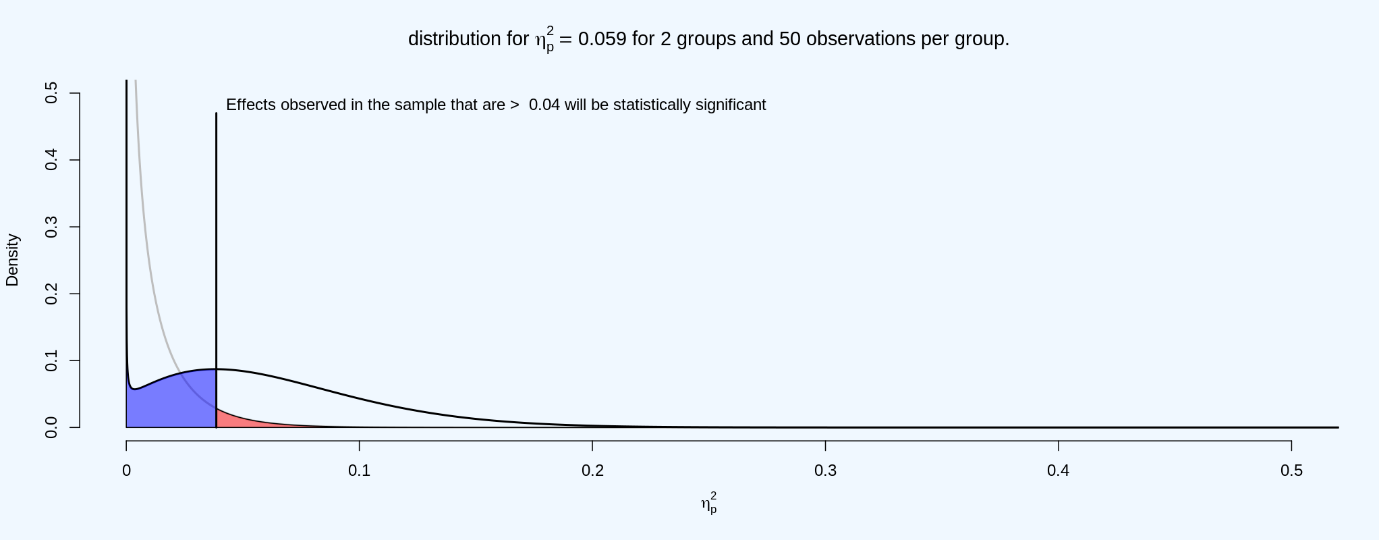
\includegraphics[width=1\textwidth,height=\textheight]{images/7f6d17dc07bdc9e95ea8944d78b16d7c.png}

}

\caption{\label{fig-critf}两组的临界\emph{F}值示意图,每组50个样本,α水平为0.05。}

\end{figure}

\textbf{问题20}:将参与者的数量(每个条件)设置为14,组的数量设置为3。使用Shiny应用程序\url{https://shiny.ieis.tue.nl/f_p_power/}看哪些效应量(以偏eta平方表示,如纵轴所示)在每组和三组n
= 14时具有统计学显著性?

\begin{enumerate}
\def\labelenumi{\Alph{enumi})}
\tightlist
\item
  仅当效应量大于0.11
\item
  仅当效应量大于0.13
\item
  仅当效应量大于0.14
\item
  仅当效应量大于0.16
\end{enumerate}

每个样本量和α水平都意味着在你的研究中具有统计显著性的最小统计可检测效应。查看你可以检测到哪些观察到的效应是一种有用的方法,可以确保你实际上可以检测到您感兴趣的最小效应大小。

\textbf{问题21}:使用最小可检测统计效应,将复现研究中的SESOI设置为\emph{d}=0.35,并将alpha水平设置为0.05。在尽可能接近原始研究的有力复现研究中收集数据后,你发现没有显著的效应,并且你可以拒绝大于或大于\emph{d}
= 0.35的影响。这个结果的正确解释是什么?

\begin{enumerate}
\def\labelenumi{\Alph{enumi})}
\tightlist
\item
  没有效应存在。
\item
  我们可以在统计上拒绝(使用0.05的alpha值)任何理论上有意义的效应。
\item
  我们可以在统计上拒绝(使用0.05的alpha值)任何实际上有意义的效应。
\item
  我们可以在统计上拒绝(使用0.05的alpha值)原始研究中有33\%的统计检验力检测到的效应。
\end{enumerate}

\hypertarget{ux5f00ux653eux6027ux95eeux9898-1}{%
\subsection{开放性问题}\label{ux5f00ux653eux6027ux95eeux9898-1}}

\begin{enumerate}
\def\labelenumi{\arabic{enumi}.}
\item
  ``没有发现证据不等于证据不存在''这句话是什么意思?
\item
  等效检验的目的是什么?
\item
  零零假设和非零零假设的区别是什么?
\item
  最小效应检验是什么?
\item
  如果对同一批数据进行零假设显著性检验和等价性检验,并且都不是显著,可以得出什么结论?
\item
  当设计等效检验以获得期望的统计检验力时,为什么需要更大的样本量,等效范围越窄?
\item
  当等效检验显著时,为什么不能说不存在效应?
\item
  设计一种方法使得贝叶斯ROPE程序和等效检验相同,并设计另一种方法使二者不同。
\item
  有哪两种方法可以使得感兴趣的效应量最小?
\item
  等效检验中''小望远镜''背后的思想是什么?
\end{enumerate}

\bookmarksetup{startatroot}

\hypertarget{sec-sequential}{%
\chapter{序列分析}\label{sec-sequential}}

在数据收集过程中反复分析传入的数据有很多好处。当研究人员可以拒绝零假设或感兴趣的最小效应量时,即使他们需要收集更多数据,或者结果显示研究有意想不到的问题(例如,被试误解指导语或问题),研究人员也可以在中期分析(interim
analysis)中停止数据收集。人们可以很容易理解,心理学研究者有道德义务重复地分析积累的数据,因为每当达到预期的置信水平,或足够清楚地表明预期的效应量不存在时,继续收集数据是对被试的时间和纳税人提供的金钱的浪费。除了这个伦理上的论点,设计利用序列分析的研究可能比只分析一次的数据更有效率,因为此时已经达到了研究者愿意收集的最大样本量。

序列分析不可与 {[}\textbf{选择性停止}{]}(optional
stopping)混淆,后者在误差控制(error
control)一章中讨论过。在选择性停止中,研究人员使用未经校正的alpha水平(如,5\%)来重复分析所得到的数据,这可能会大大增加一类错误率。与选择性停止不同,在\textbf{序列分析}中,一类错误率得到了控制。通过在每次中期分析中降低alpha水平,可以控制整体的一类错误率,就像Bonferroni校正用于防止多重比较中一类错误率的增长一样。事实上,Bonferroni校正是一个有效的(但保守的)控制序列分析的错误率的办法
(Wassmer \& Brannath, 2016)。

在序列分析中,研究者设计了一项研究,以便他们能够进行\textbf{中期分析},例如在收集了25\%、50\%和75\%的数据时。每一个中期分析都会在校正后的(corrected)alpha水平上进行检验,这样在所有计划的分析中,所需的一类错误率就会保持不变。序列分析通常用于医学试验,在医学试验中,快速发现有效的治疗方法可能是一个生死攸关的问题。如果在中期分析中,研究人员确定一种新的药物是有效的,他们很可能会想终止试验,并将有效的药物提供给对照组的患者,以改善患者的健康状况,甚至拯救他们的生命。例如,辉瑞-生物技术公司(Pfizer--BioNTech)采用了一种实验设计分析COVID-19疫苗的安全性和有效性:他们计划对数据进行5次分析,并通过降低每次中期分析的alpha水平来控制整体的一类错误率。
\href{https://www.nejm.org/doi/suppl/10.1056/NEJMoa2034577/suppl_file/nejmoa2034577_protocol.pdf}{interim
analysis}。

\begin{figure}

{\centering 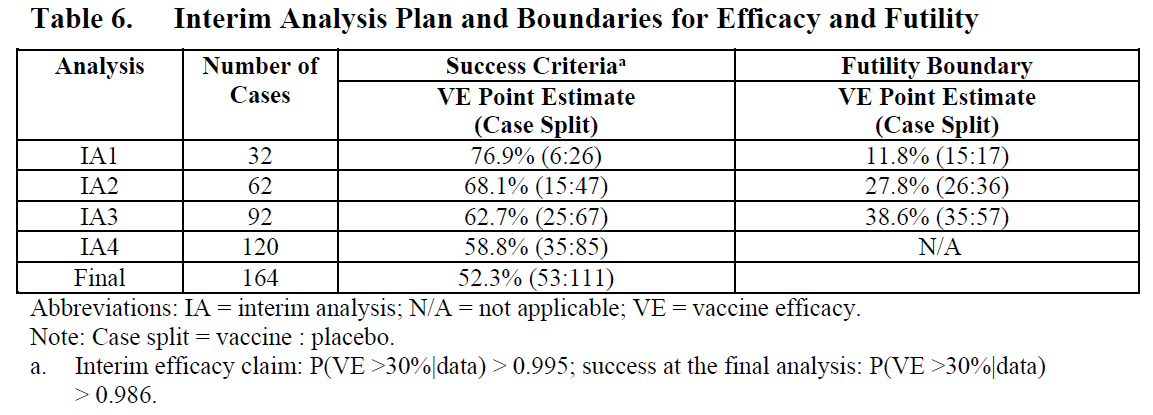
\includegraphics[width=1\textwidth,height=\textheight]{images/vaccinetrial.png}

}

\caption{用于检验BNT162b2 mRNA
Covid-19疫苗的安全性及效应的实现计划的序列分析截图}

\end{figure}

尽管序列分析技术有很长的历史,但序列分析在许多科学学科中的使用最近才慢慢变得流行起来。早在1929年,Dodge和Romig就意识到按序列分析数据比一次分析更有效率
(Dodge \& Romig, 1929)。 Wald (1945),于1945
年推广了假设的顺序检验思想,并在第二次世界大战期间开展了工作。正如他在历史记录中解释的那样,直到战争结束后他才被允许发表他的发现:

\begin{quote}
由于序列概率比试验大大节省了预期的观察次数,也由于这种试验程序在实际应用中的简单性,国防研究委员会认为这些发展对战事非常有用,所以至少在一定时期内最好不要让敌人知道这些结果。因此,作者被要求在1943年9月的一份限制性报告中提交了他的报告。
\end{quote}

序列分析是行之有效的程序,并且在过去几十年中被详细开发(Jennison \&
Turnbull, 2000; Proschan et al., 2006; Wassmer \& Brannath, 2016)。
在这里,我们将解释如何在组序列分析中(group sequential
analysis)控制错误率的基本原理,并进行先验的统计检验力分析(a-priori
power analysis),比较序列设计何时会比固定设计(fixed
designs)更高效或更低效。在我们讨论这些话题之前,有必要先了解一些术语的定义。
\textbf{观察}(look) (也称 \textbf{阶段})
是指分析截止至某一特定时间点收集的所有数据;例如,你在
50、100和150次观察之后进行观察(look),并分析到该点为止所收集的所有数据。在50次和100次观察后进行\textbf{中期分析},在第150次观察后进行\textbf{最终分析}(final
analysis),并停止数据收集。在实践中,并不是所有的观察(look)都要发生。如果分析发现在一次观察(look
1)的时候就得到了统计学意义的结果,就可以终止数据收集。我们停止的原因是拒绝\(H_0\)(例如,在无效假设显著性检验中),或者拒绝\(H_1\)(例如,在等价性检验中)。我们可以在\textbf{缩减}(curtailment)或\textbf{无用}(futility)的情况下停止分析:最终分析不可能或非常不可能产生
p \textless{} alpha的结果。序列设计中\textbf{总体alpha水平}(overall
alpha level)
与每次观察的alpha水平不同。例如,如果我们想让一个有3次观察的双侧试验的总体一类错误率为5\%,每次观察的alpha水平可以是0.0221(如果我们使用
Pocock Pocock (1977)
提出的alpha矫正方法)。在本章中,我们将重点讨论组序列设计,即在多组中收集数据,但也存在其他的序列方法,正如在关于
\protect\hyperlink{sequentialsamplesize}{sample size
justification}的章节中所解释的那样。

\hypertarget{ux4e3aux5e8fux5217ux5206ux6790ux9009ux62e9alphaux6c34ux5e73}{%
\section{为序列分析选择alpha水平}\label{ux4e3aux5e8fux5217ux5206ux6790ux9009ux62e9alphaux6c34ux5e73}}

在不校正alpha水平的情况下对数据进行多次分析时,一类错误率就会增加(Armitage
et al.,
1969)。正如Armitage和他的同事所展示的,在等间隔的观察(look)下,5次观察(look)后alpha水平会增长至0.142,100次观察(look)后增长至0.374,1000次观察(look)后增长至0.530。观测两次数据在概念上类似于决定当两个因变量中的一个显示出统计学上的显著性时,结果是否显着。然而,一个重要的区别是,在序列分析的情况下,多重检验不是独立的,而是相互依赖的。观察2的检验结合了观察1收集的旧数据和观察2的新数据。这意味着与独立测试相比,一类错误率增长的速度较慢,这使得控制错误率的解决方案更加有效和灵活。接下来我们将详细介绍。

在序列分析中控制一类错误率时,需要决定如何在所有观察数据中支出的alpha水平。例如,当研究人员计划进行一项研究,对数据进行一次中期检查和一次最终检查时,需要为第一次观察(在
\emph{N} 次观察中的 \emph{n} 个)和第二次观察(第\emph{N}
次观察)设定边界临界Z值。
需要选择这两个临界值\(c_1\)和\(c_2\)(用于第一次和第二次分析),以便拒绝零假设的总体概率(overall
probability,Pr)------在第一次分析中观察到的Z分数大于第一次观察的临界值,\(Z_n\)
≥ \(c_1\),并且(如果我们在第一次分析中没有拒绝假设,那么 \(Z_n\)
\textless{}
\(c_1\),我们继续数据收集)当在第二次分析观察到的Z分数大于第二次观察的临界值,\(Z_N\)
≥ \(c_2\) ------
当原假设为真时,等于所需的总体alpha水平。对于有方向检验(directional
test)的公式

\[
Pr\{Z_n \geq c_1\} + Pr\{Z_n < c_1, Z_N \geq c_2\} = \alpha
\]

如果有一个以上的中期分析,就必须按照同样的原理来确定额外的临界值。如果将数据的多个观察与多重比较结合起来,将对alpha水平进行两次校正,一次用于多重比较,另一次用于多个观察。因为alpha水平被校正了,所以在每次观察时进行何种统计检验方法并不重要,重要的是将\emph{p}值与校正后的alpha水平进行比较。下面讨论的校正对任何数据为正态分布的设计都是有效的,而且每一组观测值都是独立于前一组。

\hypertarget{pocockux6821ux6b63}{%
\section{Pocock校正}\label{pocockux6821ux6b63}}

研究人员需要做出的第一个决定是,如何校正跨观察的一类错误率。四种常见的方法是Pocock校正,O'Brien-Fleming校正,TheHaybittle\&Peto校正,以及Wang和Tsiatis
方法。用户也可以自由地指定他们自己喜欢的方式来支出跨观察的alpha水平。

Pocock校正是校正多次观察的alpha水平最简单的方法。从概念上讲,它与Bonferroni校正非常相似。
Pocock校正是这样被建立的:每次观察数据时的alpha水平相同,从而导致恒定的临界值(以
\emph{z} 值表示)\(u_k = c\) 以拒绝在观察\(k\)时的零假设
\(H_0\)。以下代码使用包 \texttt{rpact}来设计一个序列分析的研究:

\begin{Shaded}
\begin{Highlighting}[]
\FunctionTok{library}\NormalTok{(rpact)}
\NormalTok{design }\OtherTok{\textless{}{-}} \FunctionTok{getDesignGroupSequential}\NormalTok{(}
  \AttributeTok{kMax =} \DecValTok{2}\NormalTok{,}
  \AttributeTok{typeOfDesign =} \StringTok{"P"}\NormalTok{,}
  \AttributeTok{sided =} \DecValTok{2}\NormalTok{,}
  \AttributeTok{alpha =} \FloatTok{0.05}\NormalTok{,}
  \AttributeTok{beta =} \FloatTok{0.1}
\NormalTok{)}
\NormalTok{design}
\end{Highlighting}
\end{Shaded}

\hypertarget{design-parameters-and-output-of-group-sequential-design}{%
\section{Design parameters and output of group sequential
design}\label{design-parameters-and-output-of-group-sequential-design}}

\hypertarget{user-defined-parameters}{%
\subsection{User defined parameters}\label{user-defined-parameters}}

\begin{itemize}
\tightlist
\item
  \emph{Type of design}: Pocock
\item
  \emph{Maximum number of stages}: 2
\item
  \emph{Stages}: 1, 2
\item
  \emph{Significance level}: 0.0500
\item
  \emph{Type II error rate}: 0.1000
\item
  \emph{Test}: two-sided
\end{itemize}

\hypertarget{derived-from-user-defined-parameters}{%
\subsection{Derived from user defined
parameters}\label{derived-from-user-defined-parameters}}

\begin{itemize}
\tightlist
\item
  \emph{Information rates}: 0.500, 1.000
\end{itemize}

\hypertarget{default-parameters}{%
\subsection{Default parameters}\label{default-parameters}}

\begin{itemize}
\tightlist
\item
  \emph{Two-sided power}: FALSE
\item
  \emph{Tolerance}: 0.00000001
\end{itemize}

\hypertarget{output}{%
\subsection{Output}\label{output}}

\begin{itemize}
\tightlist
\item
  \emph{Cumulative alpha spending}: 0.02939, 0.05000
\item
  \emph{Critical values}: 2.178, 2.178
\item
  \emph{Stage levels (one-sided)}: 0.01469, 0.01469
\end{itemize}

输出结果告诉我们,使用Pocock支出函数设计一个具有两次观测(一个中期,一个最终)的研究。最后一行返回单侧的alpha水平。\texttt{rpact}
包主要应用于验证适应性临床试验设计和分析(Confirmatory Adaptive Clinical
Trial Design and
Analysis)。在临床试验中,研究人员大多检验有方向的预测,因此,默认设置是进行单侧检验。在临床试验中,通常使用0.025的显著性水平进行单侧检验,但在许多其他领域,0.05是一个更常见的默认值。我们可以通过将单侧的alpha水平乘以2来得到双侧的alpha水平:

\begin{Shaded}
\begin{Highlighting}[]
\NormalTok{design}\SpecialCharTok{$}\NormalTok{stageLevels }\SpecialCharTok{*} \DecValTok{2}
\end{Highlighting}
\end{Shaded}

\begin{verbatim}
[1] 0.02938579 0.02938579
\end{verbatim}

我们可以对照\href{https://en.wikipedia.org/wiki/Pocock_boundary}{维基百科上的
Pocock 校正页面}
检查输出结果,我们确实可以在网页上看到,在对数据进行两次观察(look)的情况下,每次观察的alpha水平是0.0294。Pocock校正比使用Bonferroni校正(在这种情况下,alpha水平将是0.025)略微有效,因为数据中存在依赖性(在第二次观察时,第一次观察时分析的数据又是分析的一部分)。

\texttt{rpact}
可以很容易地绘制出每个观察的边界(基于临界值)。观察次数被绘制成
"信息率"(Information
Rate)的函数,信息率是指在一次观测中收集的总数据的百分比。 在图
Figure~\ref{fig-boundplot1}
中有两次等距的观察,所以当50\%的数据被收集时,信息率为0.5);当100\%的数据被收集时,信息率为1。
我们看到临界值(黑色实线)大于我们在5\%
的alpha水平的固定设计中使用的1.96,即\emph{Z} =
2.178(黑色虚线)。每当我们观察到一个测试统计量在第一或第二次观察(look)时比这些临界值更极端,我们就可以拒绝零假设。

\begin{figure}

{\centering 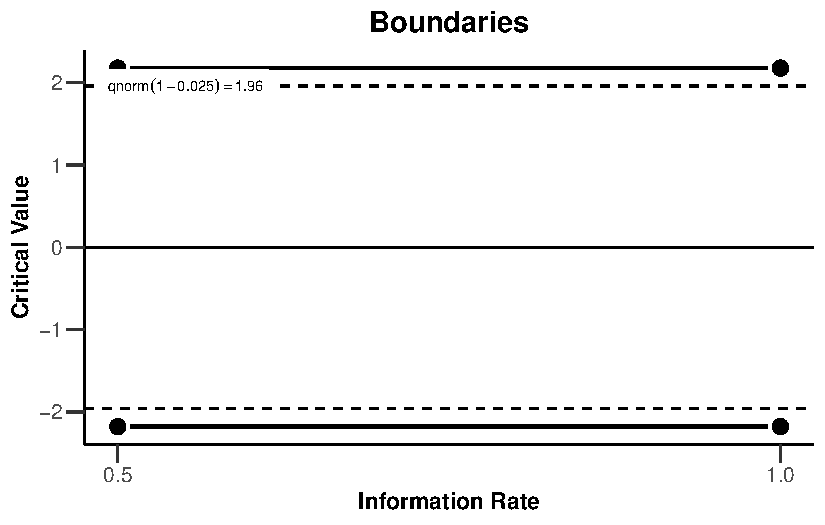
\includegraphics[width=1\textwidth,height=\textheight]{10-sequential_files/figure-pdf/fig-boundplot1-1.pdf}

}

\caption{\label{fig-boundplot1}采用Pocock校正的2次观察设计的每个观察的临界线图。}

\end{figure}

分析也可以在\texttt{rpact}\href{https://rpact.shinyapps.io/public/}{shiny
app}中进行,它也允许用户通过简单的菜单选项创建所有的图,并下载完整的分析报告(例如,用于预注册文件)。

\begin{figure}

{\centering 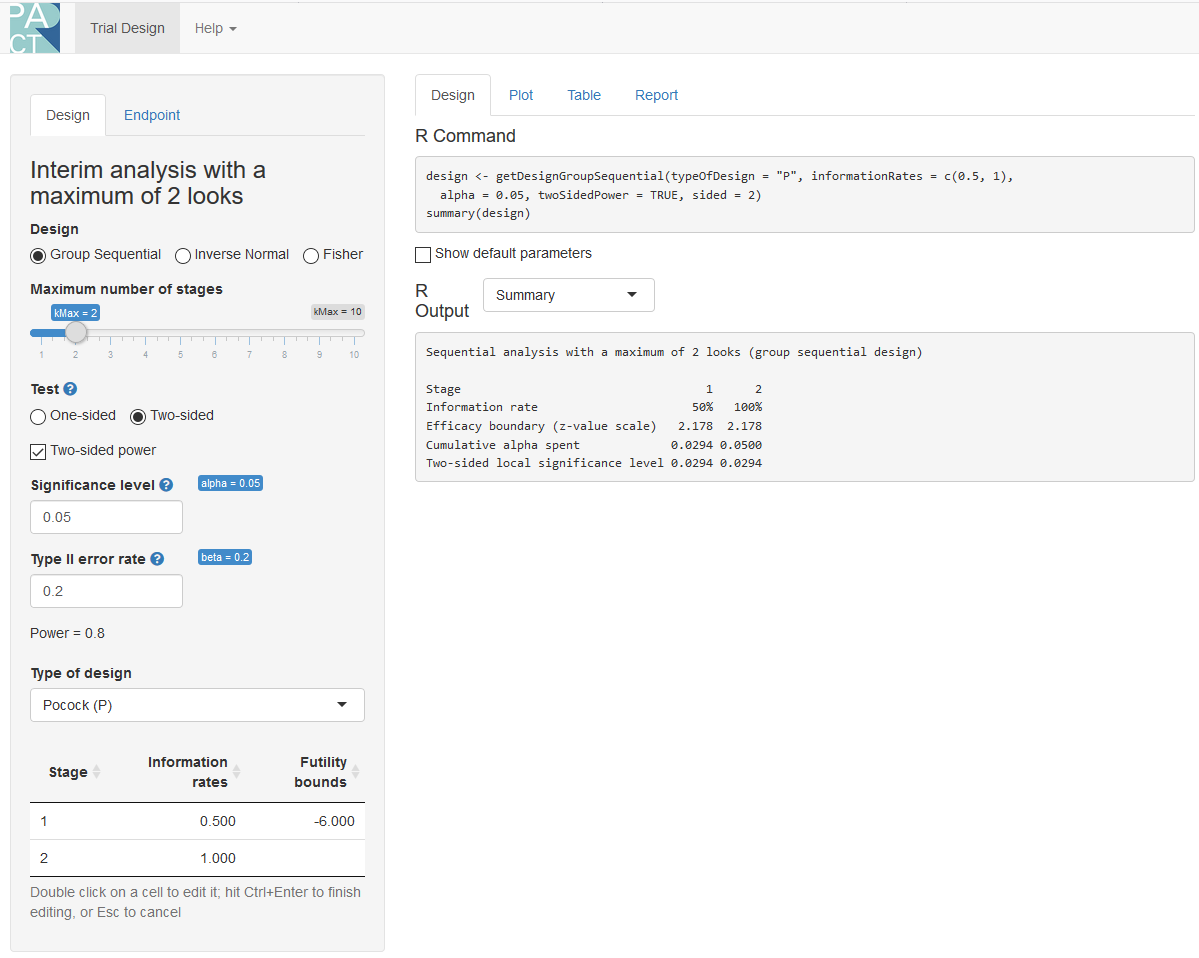
\includegraphics[width=1\textwidth,height=\textheight]{images/rpact1.png}

}

\caption{\label{fig-rpactshiny}rpact Shiny app的截图}

\end{figure}

\hypertarget{ux6bd4ux8f83ux652fux51faux51fdux6570}{%
\section{比较支出函数}\label{ux6bd4ux8f83ux652fux51faux51fdux6570}}

我们可以在同一个图中对3次观察中每一个进行不同类型的校正(两个中期和一个最终观察)(见图
Figure~\ref{fig-fourspendingfunctions})。下图展示了Pocock,O'Brien-Fleming,Haybittle-Peto和
Wang-Tsiatis对 \(\Delta\) =
0.25矫正。我们看到研究人员可以选择不同的方法来跨观察支出alpha水平。研究人员可以选择保守地使用他们的alpha(为最后一次观察保留大部分alpha),或更自由地(在早期观察中支出更多的alpha,这增加了对于许多真实效应量提前停止的可能性)。

\begin{figure}

{\centering 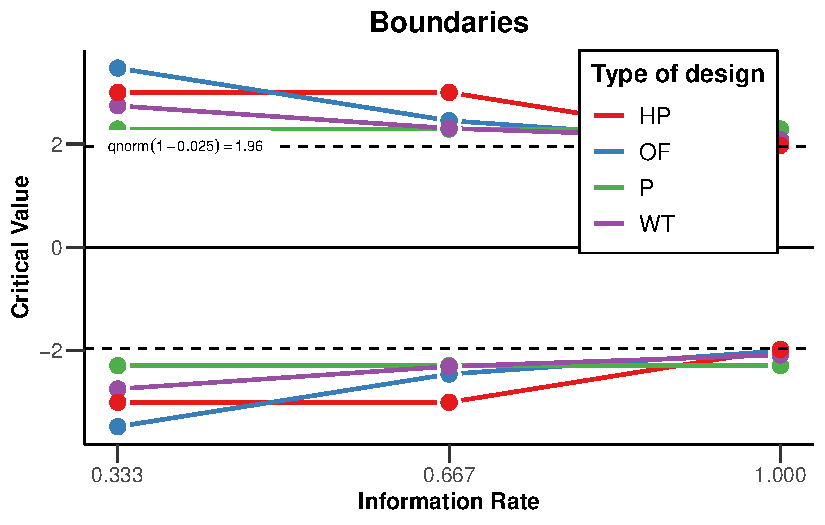
\includegraphics[width=1\textwidth,height=\textheight]{10-sequential_files/figure-pdf/fig-fourspendingfunctions-1.pdf}

}

\caption{\label{fig-fourspendingfunctions}四种不同的支出函数:
O'Brien-Fleming (OF),Pocock (P),Haybittle-Peto (HP), Wang-Tsiatis
(WT)。}

\end{figure}

我们可以看到,O'Brien和Fleming的校正在第一次观察时要保守得多,但在最后一次观察时却接近未校正的临界值1.96(见黑色虚线,对于双侧检验,所有的临界值都是反映在负方向):
3.471, 2.454, 和 2.004。 Pocock 校正在每次观察时都有相同的临界值(2.289,
2.289,以及 2.289)。The
Haybittle和Peto校正除了最后一次,在每次观察时都有相同的临界值(3, 3, and
1.975)。 而Wang和Tsiatis校正在每次观察(look) 时的临界值都会减少(2.741,
2.305, 和2.083)。

如果你主要是想监测结果的意外发展,那么在早期观察时保持保守是明智的。当效应是否存在以及效应大小有多大这两方面都存在很大的不确定性时,Pocock校正更有用,因为如果效应很大的话,它可以使提前停止实验的概率更高。因为检验的统计检验效力取决于alpha水平,在最后一次观察降低alpha水平意味着与固定设计相比统计效力降低,为了达到理想的能力,需要增加研究的样本量以保持最后观察的统计检验效力不变。样本量的增加可以通过提前停止数据收集来补偿,在这种情况下,序列设计比固定设计更有效。因为O'Brien-Fleming或Haybittle-Peto设计在最后一次观察时的alpha与只有一次观察的固定设计的统计统计检验力非常相似,所以所需的样本量也非常相似。与固定设计相比,Pocock校正需要增加更多的最大样本量以达到所需的统计检验效力。

校正后的
alpha水平可以计算到许多位数,但这很快就会达到在现实生活中毫无意义的精度水平。如果你将alpha水平设置为0.0194、0.019或0.02,那么在你一生中将进行的所有检验中观察到的一类错误率并没有明显不同(参考
\textquotesingle{}\href{https://en.wikipedia.org/wiki/Significant_figures}{significant
digits}\textquotesingle 的概念)。即使在序列测试中计算和使用alpha阈值达到许多位数,大多数研究的混乱使这些alpha水平具有虚假的精确度(\href{https://en.wikipedia.org/wiki/False_precision}{false
precision})。 在解释数据时要记住这一点。

\hypertarget{alphaux652fux51faux51fdux6570}{%
\section{Alpha支出函数}\label{alphaux652fux51faux51fdux6570}}

到目前为止,所讨论的指定不同观察(look)的决策边界形状(shape of
decision boundaries)的方法有一个重大的局限性 (Proschan et al.,
2006)。它们需要预先确定观察次数(如 4
次),而且还需要预先确定中期观察的样本量(如在 25\%、50\%、75\% 和 100\%
的观察之后)。从逻辑上讲,在计划总样本量的25\%处准确地停止数据收集并不总是可行的。Lan和DeMets
(1983)
对序列检验相关文献做出了重要贡献,他们引入了alpha支出函数来校正alpha水平。在这种方法中,通过一个函数(\emph{alpha支出函数}(alpha
spending
function))预先指定了整个观察累积的一类错误率,以控制总体显著性水平\(\alpha\)。

这些alpha支出函数的主要好处是可以控制中期分析的错误率,同时既不需要事先指定观察的次数也不需要指定时间。这使得alpha支出方法比早期的控制组序列设计中第一类错误的方法要灵活得多。使用alpha支出函数时,重要的是执行中期分析的决定不是基于收集的数据,因为这仍然会增加一类错误率。只要满足这个假设,就有可能在研究期间每次观察时更新alpha水平。

\begin{figure}

{\centering 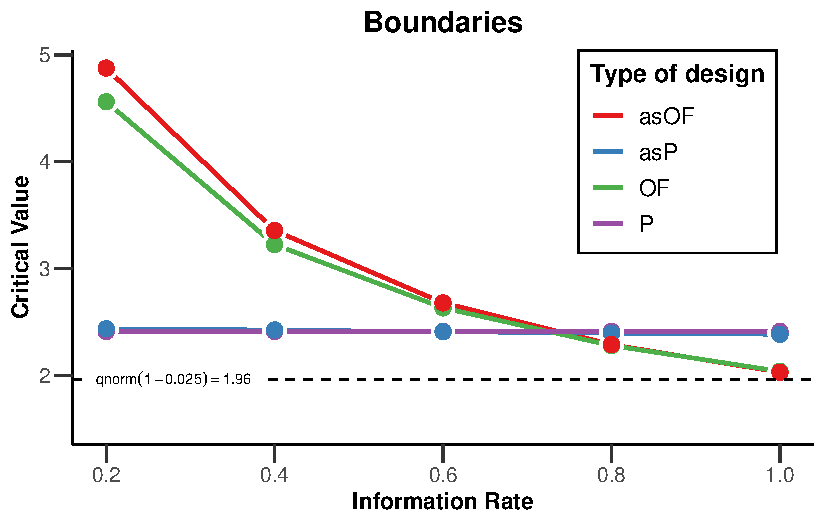
\includegraphics[width=1\textwidth,height=\textheight]{10-sequential_files/figure-pdf/fig-comparison-1.pdf}

}

\caption{\label{fig-comparison}比较五次观察中Pocock (P) and
O'Brien-Fleming correction (OF), Pocock-like (asP) and O'Brien-Fleming
like (asOF) alpha指出函数。}

\end{figure}

\hypertarget{ux5728ux7814ux7a76ux671fux95f4ux66f4ux65b0ux8fb9ux754c}{%
\section{在研究期间更新边界}\label{ux5728ux7814ux7a76ux671fux95f4ux66f4ux65b0ux8fb9ux754c}}

尽管即使是在偏离预先计划的观察次数或时间的情况下,alpha支出函数控制了第一类错误率,这确实需要根据已经观察到的信息量重新计算统计检验中使用的边界。让我们假设一个研究者设计了一项研究,对数据进行三次等距的观察(两次中期观察,一次最终观察),使用Pocock类型的alpha支出函数,结果将以双侧\emph{t}检验的方式进行分析,总体期望的一类错误率为0.05,期望的统计检验效力为0.9,Cohen's
\emph{d} 为0.5。一个先验的统计检验效力分析(a-priori power
analysis,我们将在下一节解释)表明,如果我们计划在每个条件下观测65.4、130.9和196.3个观测值,我们在序列设计中就能达到预期的统计检验效力。由于被试个数为整数且有2个独立的小组,我们应该将上述数字四舍五入后分为两组,我们将在第一轮观察时收集66个观察值(每组33个),在第二轮观察时收集132个(每组66个),在第三轮观察时收集198个(每组99个)。下面的代码将计算每一个观察(look
或阶段)的alpha水平,以进行双侧检验:

\begin{Shaded}
\begin{Highlighting}[]
\NormalTok{design }\OtherTok{\textless{}{-}} \FunctionTok{getDesignGroupSequential}\NormalTok{(}\AttributeTok{kMax =} \DecValTok{3}\NormalTok{, }
                                   \AttributeTok{typeOfDesign =} \StringTok{"asP"}\NormalTok{,}
                                   \AttributeTok{sided =} \DecValTok{2}\NormalTok{, }
                                   \AttributeTok{alpha =} \FloatTok{0.05}\NormalTok{, }
                                   \AttributeTok{beta =} \FloatTok{0.1}\NormalTok{)}
\NormalTok{design}\SpecialCharTok{$}\NormalTok{stageLevels }\SpecialCharTok{*} \DecValTok{2}
\end{Highlighting}
\end{Shaded}

\begin{verbatim}
[1] 0.02264162 0.02173822 0.02167941
\end{verbatim}

现在想象一下,由于后勤问题(A logistical problem \textbf{occurs when
your plans didn't account for
something}),我们在收集了76个观测值(每个条件38个)而不是计划的66个观测值的数据后,才设法分析数据。这样的后勤问题在实践中很常见,也是alpha支出函数为组序列设计而开发的主要原因之一。与计划不同,我们对数据的第一次观察并不是在收集总样本的33.3\%的时候发生的,而是在达到76/198=38.4\%个计划样本的时候发生的。我们可以根据当前的观察和未来计划的观察,重新计算每次观察数据时应该使用的alpha水平。而不是在三次观察时分别使用如上面所计算的0.0226、0.0217和0.0217的alpha水平(注意在类似Pocock的alpha支出函数中,alpha水平在每次观察时几乎相同,但不完全相同,不像Pocock校正,它们在每次观察时是相同的)。我们可以通过在下面的代码中使用\texttt{informationRates}明确指定信息率来校正它们。现在,第一次观察发生在计划样本的76/198处;第二次观察仍计划在样本的2/3处发生;最后一次观察在计划的最大样本量处。

\begin{Shaded}
\begin{Highlighting}[]
\NormalTok{design }\OtherTok{\textless{}{-}} \FunctionTok{getDesignGroupSequential}\NormalTok{(}
  \AttributeTok{typeOfDesign =} \StringTok{"asP"}\NormalTok{, }
  \AttributeTok{informationRates =} \FunctionTok{c}\NormalTok{(}\DecValTok{76}\SpecialCharTok{/}\DecValTok{198}\NormalTok{, }\DecValTok{2}\SpecialCharTok{/}\DecValTok{3}\NormalTok{, }\DecValTok{1}\NormalTok{), }
  \AttributeTok{alpha =} \FloatTok{0.05}\NormalTok{, }
  \AttributeTok{sided =} \DecValTok{2}\NormalTok{)}
\NormalTok{design}\SpecialCharTok{$}\NormalTok{stageLevels }\SpecialCharTok{*} \DecValTok{2}
\end{Highlighting}
\end{Shaded}

\begin{verbatim}
[1] 0.02532710 0.02043978 0.02164755
\end{verbatim}

更新后的alpha水平是:当前观察(look)为0.0253,第二次观察(look)为0.0204,最后一次观察(look)为0.0216。因此,第一次观察(look)中使用的alpha水平不是0.0226(按照最初的计划),而是稍高的0.0253。第二次观察将使用略低的alpha值0.0204,而不是0.0217。虽然差异很小,但事实上有一种正式的方法来控制alpha水平,可以灵活地查看与最初计划不同的时间,这一点非常有用。

如果最后观察的数据发生了变化,例如因为你无法收集到预定的样本量,或者由于其他不可预见的情况,你收集到的数据比计划的多,也可以校正alpha水平。由于研究者预注册了他们的研究,或使用注册报告发表,这种情况越来越普遍。有时他们最终得到的数据比计划的略多,这就出现了一个问题:他们应该用计划的样本量进行分析,还是分析所有的数据。分析所有收集到的数据可以防止浪费被试的应答,并使用所有可用的信息,但它增加了数据分析的灵活性(因为研究人员现在可以选择分析计划中的样本数据,或者分析他们收集到的所有数据)。Alpha支出函数使得研究人员可以分析所有数据,同时更新用于控制整体alpha水平的alpha水平来解决这个难题。

如果收集的数据比计划的多,我们就不能再使用被选择的alpha支出函数(即Pocock支出函数),而必须通过更新时间和alpha支出函数来提供一个\textbf{用户定义的alpha支出函数}(user-defined
alpha spending
function),以反映最后一次观察时实际发生的数据收集情况。假设在我们前面的例子中,第二次观察按原计划发生在计划收集的数据的2/3处,但最后一次观察发生在206个被试时,而不是198个被试时,我们可以计算出最后一次观察的最新alpha水平。考虑到目前的总样本量,我们需要重新计算早期观察的alpha水平,现在发生在76/206=0.369,132/206=0.641,最后一次观察是206/206=1。

第一次和第二次观察发生在我们第一次校正后计算出的校正后的alpha水平(alpha水平为0.0253和0.0204)。我们已经在前两次观察的时候支出了我们总alpha的一部分。我们可以看一下我们上面指定的设计结果中的''累计alpha支出''(Cumulative
alpha spent),看看到目前为止我们支出了多少一类错误率:

\begin{Shaded}
\begin{Highlighting}[]
\NormalTok{design}\SpecialCharTok{$}\NormalTok{alphaSpent}
\end{Highlighting}
\end{Shaded}

\begin{verbatim}
[1] 0.02532710 0.03816913 0.05000000
\end{verbatim}

我们看到我们在第一次观察后支出了0.0253,第二次观察后支出了0.0382。由此可知,在最后一次观察时支出我们一类错误率的剩余部分,总共是0.05。

在收集了比计划中更多的数据后,我们的实际alpha支出函数不再被Pocock支出函数所获取,因此改为指定一个用户定义的支出函数。我们可以在设定\texttt{asUser}设计后,通过设定\texttt{userAlphaSpending}
信息,使用下面的代码进行这些计算:

\begin{Shaded}
\begin{Highlighting}[]
\NormalTok{design }\OtherTok{\textless{}{-}} \FunctionTok{getDesignGroupSequential}\NormalTok{(}
  \AttributeTok{typeOfDesign =} \StringTok{"asUser"}\NormalTok{, }
  \AttributeTok{informationRates =} \FunctionTok{c}\NormalTok{(}\DecValTok{72}\SpecialCharTok{/}\DecValTok{206}\NormalTok{, }\DecValTok{132}\SpecialCharTok{/}\DecValTok{206}\NormalTok{, }\DecValTok{1}\NormalTok{), }
  \AttributeTok{alpha =} \FloatTok{0.05}\NormalTok{, }
  \AttributeTok{sided =} \DecValTok{2}\NormalTok{, }
  \AttributeTok{userAlphaSpending =} \FunctionTok{c}\NormalTok{(}\FloatTok{0.0253}\NormalTok{, }\FloatTok{0.0382}\NormalTok{, }\FloatTok{0.05}\NormalTok{)}
\NormalTok{)}
\NormalTok{design}\SpecialCharTok{$}\NormalTok{stageLevels }\SpecialCharTok{*} \DecValTok{2}
\end{Highlighting}
\end{Shaded}

\begin{verbatim}
[1] 0.02530000 0.01987072 0.02075796
\end{verbatim}

之前观察的alpha水平与我们使用的alpha水平不一致,但最终的alpha水平(0.0208)给出了我们应该用于最终分析的alpha水平,基于比我们计划收集的样本量更大的样本量。如果我们收集了计划中的样本量,与我们会使用的alpha水平的差异确实较小(0.0216对0.0208),部分原因是所收集的样本量与我们计划的样本量差异较小。在实践中,这种alpha水平的小差异其实并不明显,但有一个正确的解决方案来处理收集比计划多的数据,同时控制一类错误率是非常有用的。如果使用序列设计,每当超额完成预注册中计划收集的样本量时,可以使用这些方法去校正。

\hypertarget{ux5e8fux5217ux8bbeux8ba1ux7684ux6837ux672cux91cf}{%
\section{序列设计的样本量}\label{ux5e8fux5217ux8bbeux8ba1ux7684ux6837ux672cux91cf}}

在最终观察时,与固定设计相比,序列设计是否需要更多的被试,取决于多重比较校正导致该次观察的alpha水平降低了多少。由于可以提前停止收集数据,序列设计平均需要更少的被试。首先,让我们检查在固定设计中我们需要多少被试,我们只分析一次数据。我们的alpha水平为0.05,二类(beta)错误为0.1,换句话说,所需的统计检验效力为90\%。我们将执行一项检验,假定数据服从正态分布,我们的临界Z分数将为1.96,alpha水平为5\%。

\begin{Shaded}
\begin{Highlighting}[]
\NormalTok{design }\OtherTok{\textless{}{-}} \FunctionTok{getDesignGroupSequential}\NormalTok{(}
  \AttributeTok{kMax =} \DecValTok{1}\NormalTok{,}
  \AttributeTok{typeOfDesign =} \StringTok{"P"}\NormalTok{,}
  \AttributeTok{sided =} \DecValTok{2}\NormalTok{,}
  \AttributeTok{alpha =} \FloatTok{0.05}\NormalTok{,}
  \AttributeTok{beta =} \FloatTok{0.1}
\NormalTok{)}

\NormalTok{power\_res }\OtherTok{\textless{}{-}} \FunctionTok{getSampleSizeMeans}\NormalTok{(}
  \AttributeTok{design =}\NormalTok{ design,}
  \AttributeTok{groups =} \DecValTok{2}\NormalTok{,}
  \AttributeTok{alternative =} \FloatTok{0.5}\NormalTok{, }
  \AttributeTok{stDev =} \DecValTok{1}\NormalTok{, }
  \AttributeTok{allocationRatioPlanned =} \DecValTok{1}\NormalTok{,}
  \AttributeTok{normalApproximation =} \ConstantTok{FALSE}\NormalTok{)}

\NormalTok{power\_res}
\end{Highlighting}
\end{Shaded}

\hypertarget{design-plan-parameters-and-output-for-means}{%
\section{Design plan parameters and output for
means}\label{design-plan-parameters-and-output-for-means}}

\hypertarget{design-parameters}{%
\subsection{Design parameters}\label{design-parameters}}

\begin{itemize}
\tightlist
\item
  \emph{Critical values}: 1.96
\item
  \emph{Two-sided power}: FALSE
\item
  \emph{Significance level}: 0.0500
\item
  \emph{Type II error rate}: 0.1000
\item
  \emph{Test}: two-sided
\end{itemize}

\hypertarget{user-defined-parameters-1}{%
\subsection{User defined parameters}\label{user-defined-parameters-1}}

\begin{itemize}
\tightlist
\item
  \emph{Alternatives}: 0.5
\end{itemize}

\hypertarget{default-parameters-1}{%
\subsection{Default parameters}\label{default-parameters-1}}

\begin{itemize}
\tightlist
\item
  \emph{Mean ratio}: FALSE
\item
  \emph{Theta H0}: 0
\item
  \emph{Normal approximation}: FALSE
\item
  \emph{Standard deviation}: 1
\item
  \emph{Treatment groups}: 2
\item
  \emph{Planned allocation ratio}: 1
\end{itemize}

\hypertarget{sample-size-and-output}{%
\subsection{Sample size and output}\label{sample-size-and-output}}

\begin{itemize}
\tightlist
\item
  \emph{Number of subjects fixed}: 170.1
\item
  \emph{Number of subjects fixed (1)}: 85
\item
  \emph{Number of subjects fixed (2)}: 85
\item
  \emph{Lower critical values (treatment effect scale)}: -0.303
\item
  \emph{Upper critical values (treatment effect scale)}: 0.303
\item
  \emph{Local two-sided significance levels}: 0.0500
\end{itemize}

\hypertarget{legend}{%
\subsection{Legend}\label{legend}}

\begin{itemize}
\tightlist
\item
  \emph{(i)}: values of treatment arm i
\end{itemize}

我们看到每组需要 85 名被试,(或 86 名,因为样本量实际上是 85.03
,所需的观察值是四舍五入取整的,所以我们总共需要 172
名被试。其他统计检验效力分析软件,如G*Power,也会得出同样的所需样本量。我们现在可以用两次观察和一个类似Pocock的alpha支出函数来检验我们上面的设计,即一个alpha为0.05的双侧检验。我们将观察两次,预期真实效果为\emph{d}=0.5(通过设定alternative为0.5,stDev为1)。

\begin{Shaded}
\begin{Highlighting}[]
\NormalTok{seq\_design }\OtherTok{\textless{}{-}} \FunctionTok{getDesignGroupSequential}\NormalTok{(}
  \AttributeTok{kMax =} \DecValTok{2}\NormalTok{,}
  \AttributeTok{typeOfDesign =} \StringTok{"asP"}\NormalTok{,}
  \AttributeTok{sided =} \DecValTok{2}\NormalTok{,}
  \AttributeTok{alpha =} \FloatTok{0.05}\NormalTok{,}
  \AttributeTok{beta =} \FloatTok{0.1}
\NormalTok{  )}

\CommentTok{\# Compute the sample size we need}
\NormalTok{power\_res\_seq }\OtherTok{\textless{}{-}} \FunctionTok{getSampleSizeMeans}\NormalTok{(}
  \AttributeTok{design =}\NormalTok{ seq\_design,}
  \AttributeTok{groups =} \DecValTok{2}\NormalTok{,}
  \AttributeTok{alternative =} \FloatTok{0.5}\NormalTok{, }
  \AttributeTok{stDev =} \DecValTok{1}\NormalTok{, }
  \AttributeTok{allocationRatioPlanned =} \DecValTok{1}\NormalTok{,}
  \AttributeTok{normalApproximation =} \ConstantTok{FALSE}\NormalTok{)}

\NormalTok{power\_res\_seq}
\end{Highlighting}
\end{Shaded}

\hypertarget{design-plan-parameters-and-output-for-means-1}{%
\section{Design plan parameters and output for
means}\label{design-plan-parameters-and-output-for-means-1}}

\hypertarget{design-parameters-1}{%
\subsection{Design parameters}\label{design-parameters-1}}

\begin{itemize}
\tightlist
\item
  \emph{Information rates}: 0.500, 1.000
\item
  \emph{Critical values}: 2.157, 2.201
\item
  \emph{Futility bounds (non-binding)}: -Inf
\item
  \emph{Cumulative alpha spending}: 0.03101, 0.05000
\item
  \emph{Local one-sided significance levels}: 0.01550, 0.01387
\item
  \emph{Two-sided power}: FALSE
\item
  \emph{Significance level}: 0.0500
\item
  \emph{Type II error rate}: 0.1000
\item
  \emph{Test}: two-sided
\end{itemize}

\hypertarget{user-defined-parameters-2}{%
\subsection{User defined parameters}\label{user-defined-parameters-2}}

\begin{itemize}
\tightlist
\item
  \emph{Alternatives}: 0.5
\end{itemize}

\hypertarget{default-parameters-2}{%
\subsection{Default parameters}\label{default-parameters-2}}

\begin{itemize}
\tightlist
\item
  \emph{Mean ratio}: FALSE
\item
  \emph{Theta H0}: 0
\item
  \emph{Normal approximation}: FALSE
\item
  \emph{Standard deviation}: 1
\item
  \emph{Treatment groups}: 2
\item
  \emph{Planned allocation ratio}: 1
\end{itemize}

\hypertarget{sample-size-and-output-1}{%
\subsection{Sample size and output}\label{sample-size-and-output-1}}

\begin{itemize}
\tightlist
\item
  \emph{Reject per stage {[}1{]}}: 0.6022
\item
  \emph{Reject per stage {[}2{]}}: 0.2978
\item
  \emph{Early stop}: 0.6022
\item
  \emph{Maximum number of subjects}: 188.9
\item
  \emph{Maximum number of subjects (1)}: 94.5
\item
  \emph{Maximum number of subjects (2)}: 94.5
\item
  \emph{Number of subjects {[}1{]}}: 94.5
\item
  \emph{Number of subjects {[}2{]}}: 188.9
\item
  \emph{Expected number of subjects under H0}: 186
\item
  \emph{Expected number of subjects under H0/H1}: 172.7
\item
  \emph{Expected number of subjects under H1}: 132.1
\item
  \emph{Lower critical values (treatment effect scale) {[}1{]}}: -0.451
\item
  \emph{Lower critical values (treatment effect scale) {[}2{]}}: -0.323
\item
  \emph{Upper critical values (treatment effect scale) {[}1{]}}: 0.451
\item
  \emph{Upper critical values (treatment effect scale) {[}2{]}}: 0.323
\item
  \emph{Local two-sided significance levels {[}1{]}}: 0.03101
\item
  \emph{Local two-sided significance levels {[}2{]}}: 0.02774
\end{itemize}

\hypertarget{legend-1}{%
\subsection{Legend}\label{legend-1}}

\begin{itemize}
\tightlist
\item
  \emph{(i)}: values of treatment arm i
\item
  \emph{{[}k{]}}: values at stage k
\end{itemize}

第一次观测每个小组的样本量是 47.24 47.24,第二次观测是 94.47
94.47,这意味着我们现在收集了 190 而不是 172
个被试。这是每次观察降低alpha水平(从0.05到 0.028)的结果。
为了补偿每次降低的alpha水平,我们需要增加研究的样本量以达到相同的统计检验效力。

然而,最大的样本量并不是这种设计的预期样本量,因为我们有可能在序列设计中的较早的观察点上停止数据收集。从长远来看,如果\emph{d}=0.5,我们使用Pocock类型的alpha支出函数,并忽略向上取整,因为我们只能收集一个完整的观测值,我们有时会收集
96 个被试,并在第一次观察后停止,其余时间继续收集 190 名被试。
正如我们在'Reject per stage'这一行中所看到的一样,第一次观察预计在研究的
0.6 停止,因为我们已经观察到一个显著的结果。 剩余的时间是 (1 - 0.6) =
0.4.

这意味着假设存在 \emph{d} = 0.5的真实效应, 平均\emph{期待}
的平均样本量是在每次观察时停止的概率乘以我们每次观察时收集的观测值数量,即
0.6 * 96 + 0.3 * 190 = 133.39. \texttt{rpact} 包在''\(H_1\)
下的预期受试者数量''下返回的数值为 132.06 - 微小的差异是由于
\texttt{rpact} 没有将观测值数量四舍五入)。 因此,假设真实效应量为
\emph{d} = 0.5,
在任何一项研究中,我们可能需要收集比固定设计略多的数据(我们将收集
172),但平均而言,我们在序列设计中需要收集的观察数量更小。

因为统计检验效力是一条曲线,而真实的效应值是未知的,所以绘制一系列可能的效应值的统计检验效力可以有所帮助,这样我们就可以探索不同的真实效应值的预期样本量。

\begin{Shaded}
\begin{Highlighting}[]
\CommentTok{\# Use getPowerMeans and set max N to 190 based on analysis above}
\NormalTok{sample\_res }\OtherTok{\textless{}{-}} \FunctionTok{getPowerMeans}\NormalTok{(}
  \AttributeTok{design =}\NormalTok{ seq\_design,}
  \AttributeTok{groups =} \DecValTok{2}\NormalTok{,}
  \AttributeTok{alternative =} \FunctionTok{seq}\NormalTok{(}\DecValTok{0}\NormalTok{, }\DecValTok{1}\NormalTok{, }\FloatTok{0.01}\NormalTok{), }
  \AttributeTok{stDev =} \DecValTok{1}\NormalTok{, }
  \AttributeTok{allocationRatioPlanned =} \DecValTok{1}\NormalTok{,}
  \AttributeTok{maxNumberOfSubjects =} \DecValTok{190}\NormalTok{, }
  \AttributeTok{normalApproximation =} \ConstantTok{FALSE}\NormalTok{)}

\FunctionTok{plot}\NormalTok{(sample\_res, }\AttributeTok{type =} \DecValTok{6}\NormalTok{)}
\end{Highlighting}
\end{Shaded}

\begin{figure}[H]

{\centering 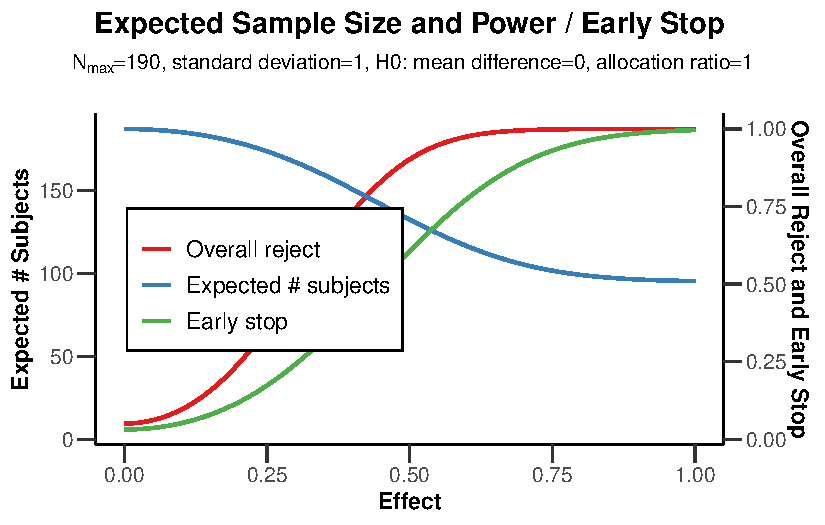
\includegraphics[width=1\textwidth,height=\textheight]{10-sequential_files/figure-pdf/fig-powerseq-1.pdf}

}

\caption{\label{fig-powerseq}两次观察的序列分析统计统计检验力图。}

\end{figure}

图 Figure~\ref{fig-powerseq}
中的蓝线表示我们需要收集的预期观测值的数量。毫不奇怪,当真正的效应值为0时,我们几乎总是会继续收集数据到最后。只有当观察到一类错误时,我们才会停止,而第一类错误是很少见的,因此,预期的观察数非常接近于我们想要收集的最大样本量。在图的另一边,我们看到了真实效应值为\emph{d}=1时的情况。有了这么大的效应值,我们在第一次观察时就会有很高的统计检验效力,而且我们几乎总是能够在第一次观察时就停下来。红线表示最后一次观察的统计检验效力,绿线表示提前停止的概率。

Pocock
校正导致最后一次观察时的alpha水平大幅降低,这需要增加样本量来补偿。正如我们之前所看到的,O'Brien-Fleming
支出函数不需要在最后一次观察时大幅降低alpha水平。正如下面的统计检验效力分析所显示的,在两次观察的情况下,这种设计在实践中根本不需要增加样本量。

\begin{Shaded}
\begin{Highlighting}[]
\NormalTok{seq\_design }\OtherTok{\textless{}{-}} \FunctionTok{getDesignGroupSequential}\NormalTok{(}
  \AttributeTok{kMax =} \DecValTok{2}\NormalTok{,}
  \AttributeTok{typeOfDesign =} \StringTok{"asOF"}\NormalTok{,}
  \AttributeTok{sided =} \DecValTok{2}\NormalTok{,}
  \AttributeTok{alpha =} \FloatTok{0.05}\NormalTok{,}
  \AttributeTok{beta =} \FloatTok{0.1}
\NormalTok{  )}

\CommentTok{\# Compute the sample size we need}
\NormalTok{power\_res\_seq }\OtherTok{\textless{}{-}} \FunctionTok{getSampleSizeMeans}\NormalTok{(}
  \AttributeTok{design =}\NormalTok{ seq\_design,}
  \AttributeTok{groups =} \DecValTok{2}\NormalTok{,}
  \AttributeTok{alternative =} \FloatTok{0.5}\NormalTok{, }
  \AttributeTok{stDev =} \DecValTok{1}\NormalTok{, }
  \AttributeTok{allocationRatioPlanned =} \DecValTok{1}\NormalTok{,}
  \AttributeTok{normalApproximation =} \ConstantTok{FALSE}\NormalTok{)}

\FunctionTok{summary}\NormalTok{(power\_res\_seq)}
\end{Highlighting}
\end{Shaded}

\hypertarget{sample-size-calculation-for-a-continuous-endpoint}{%
\section{Sample size calculation for a continuous
endpoint}\label{sample-size-calculation-for-a-continuous-endpoint}}

Sequential analysis with a maximum of 2 looks (group sequential design),
overall significance level 5\% (two-sided). The sample size was
calculated for a two-sample t-test, H0: mu(1) - mu(2) = 0, H1: effect =
0.5, standard deviation = 1, power 90\%.

\begin{longtable}[]{@{}lll@{}}
\toprule\noalign{}
Stage & 1 & 2 \\
\midrule\noalign{}
\endhead
\bottomrule\noalign{}
\endlastfoot
Information rate & 50\% & 100\% \\
Efficacy boundary (z-value scale) & 2.963 & 1.969 \\
Overall power & 0.2525 & 0.9000 \\
Expected number of subjects & 149.1 & \\
Number of subjects & 85.3 & 170.6 \\
Cumulative alpha spent & 0.0031 & 0.0500 \\
Two-sided local significance level & 0.0031 & 0.0490 \\
Lower efficacy boundary (t) & -0.661 & -0.304 \\
Upper efficacy boundary (t) & 0.661 & 0.304 \\
Exit probability for efficacy (under H0) & 0.0031 & \\
Exit probability for efficacy (under H1) & 0.2525 & \\
\end{longtable}

Legend:

\begin{itemize}
\tightlist
\item
  \emph{(t)}: treatment effect scale
\end{itemize}

\begin{center}\rule{0.5\linewidth}{0.5pt}\end{center}

\hypertarget{design-plan-parameters-and-output-for-means-2}{%
\section{Design plan parameters and output for
means}\label{design-plan-parameters-and-output-for-means-2}}

\hypertarget{design-parameters-2}{%
\subsection{Design parameters}\label{design-parameters-2}}

\begin{itemize}
\tightlist
\item
  \emph{Information rates}: 0.500, 1.000
\item
  \emph{Critical values}: 2.963, 1.969
\item
  \emph{Futility bounds (non-binding)}: -Inf
\item
  \emph{Cumulative alpha spending}: 0.003051, 0.050000
\item
  \emph{Local one-sided significance levels}: 0.001525, 0.024500
\item
  \emph{Two-sided power}: FALSE
\item
  \emph{Significance level}: 0.0500
\item
  \emph{Type II error rate}: 0.1000
\item
  \emph{Test}: two-sided
\end{itemize}

\hypertarget{user-defined-parameters-3}{%
\subsection{User defined parameters}\label{user-defined-parameters-3}}

\begin{itemize}
\tightlist
\item
  \emph{Alternatives}: 0.5
\end{itemize}

\hypertarget{default-parameters-3}{%
\subsection{Default parameters}\label{default-parameters-3}}

\begin{itemize}
\tightlist
\item
  \emph{Mean ratio}: FALSE
\item
  \emph{Theta H0}: 0
\item
  \emph{Normal approximation}: FALSE
\item
  \emph{Standard deviation}: 1
\item
  \emph{Treatment groups}: 2
\item
  \emph{Planned allocation ratio}: 1
\end{itemize}

\hypertarget{sample-size-and-output-2}{%
\subsection{Sample size and output}\label{sample-size-and-output-2}}

\begin{itemize}
\tightlist
\item
  \emph{Reject per stage {[}1{]}}: 0.2525
\item
  \emph{Reject per stage {[}2{]}}: 0.6475
\item
  \emph{Early stop}: 0.2525
\item
  \emph{Maximum number of subjects}: 170.6
\item
  \emph{Maximum number of subjects (1)}: 85.3
\item
  \emph{Maximum number of subjects (2)}: 85.3
\item
  \emph{Number of subjects {[}1{]}}: 85.3
\item
  \emph{Number of subjects {[}2{]}}: 170.6
\item
  \emph{Expected number of subjects under H0}: 170.4
\item
  \emph{Expected number of subjects under H0/H1}: 167.7
\item
  \emph{Expected number of subjects under H1}: 149.1
\item
  \emph{Lower critical values (treatment effect scale) {[}1{]}}: -0.661
\item
  \emph{Lower critical values (treatment effect scale) {[}2{]}}: -0.304
\item
  \emph{Upper critical values (treatment effect scale) {[}1{]}}: 0.661
\item
  \emph{Upper critical values (treatment effect scale) {[}2{]}}: 0.304
\item
  \emph{Local two-sided significance levels {[}1{]}}: 0.003051
\item
  \emph{Local two-sided significance levels {[}2{]}}: 0.049000
\end{itemize}

\hypertarget{legend-2}{%
\subsection{Legend}\label{legend-2}}

\begin{itemize}
\tightlist
\item
  \emph{(i)}: values of treatment arm i
\item
  \emph{{[}k{]}}: values at stage k
\end{itemize}

当我们收集到 172
名被试时这种设计就达到了预期的检验力--与我们\emph{不}观察数据时的人数完全一致。
我们基本上可以自由获取观察数据,即预期的被试数量(假设\emph{d}=0.5)下降到
149.1。
把观察(look)的次数增加到4次,只需要增加很小的被试数量就可以保持相同的统计检验力,但却进一步减少了预期的样本量。特别是对于保守的先验统计检验效力分析(a-priori
power
analysis),或对目标最小效应量进行先验统计检验效力分析时,而真正的效应值有相当大的可能性时,使用序列分析是一个非常有吸引力的选择。

\hypertarget{ux65e0ux6548ux505cux6b62}{%
\section{无效停止}\label{ux65e0ux6548ux505cux6b62}}

到目前为止,我们所讨论的序列设计只有在能够拒绝\(H_0\)的情况下才会在中期分析时停止。一个设计严谨的研究也会考虑到不存在效应的可能性,正如我们在
\protect\hyperlink{equivalencetest}{等价性检验}一章中所讨论的。在序列分析文献中,为拒绝目标最小效应值的存在而停止的做法,被称为\textbf{停止无效}
(stopping for
futility)。在最极端的情况下,在中期分析之后,也许不可能在最终分析时产生统计学上的显著结果。为了在一个假设的情况下说明这一点,设想在收集了192个观察值中的182个后,观察到的两个独立组别之间的平均差值是0.1,而研究的设计理念是认为值得的最小效应是0.5的平均差值。如果主要因变量是用7分的李克特量表测量的,那么即使对照组下剩下的5个被试都回答1,而实验组下剩下的被试都回答7,192次观察后的效应量也不会产生
\emph{p} \textless{}
\(\alpha\)。如果你的研究目标是检测是否存在至少0.5的平均差值的影响,此时研究人员知道该目标将无法实现。由于最终结果无法产生显着影响,而在中期分析时停止研究称为\emph{非随机缩减}
(non-stochastic curtailment)。

在不太极端但更普遍的情况下,研究仍有可能观察到显著效应,但概率可能非常小。考虑到已经观察到的到中期分析的数据,找到一个显著结果的概率被称为\textbf{条件功效}(conditional
power)。对最初预期的效应值进行条件功效分析可能过于乐观,但使用观察到的效应值也是不可取的,因为它通常具有相当大的不确定性。一种建议是根据观察到的数据来更新校正预期的效应值。如果使用贝叶斯更新过程,这被称为\textbf{预测能力}
(predictive power) (Spiegelhalter et al.,
1986)。可以使用\textbf{自适应设计}(adaptive
designs),允许研究者根据中期分析结果增加最终的观察数量,而不增加一类错误率(见
Wassmer \& Brannath (2016))。

另外,如果观察到的效应值比预期的要小,人们可能会因无用而停止。作为一个简单的无效性停止规则的说明,设想一个研究者,只要观察到的效应值为零,或者观察到的效应值与预测的方向相反,就会因无效而停止。在图
Figure~\ref{fig-futility1}
中,红线表示证实效应显著的临界值。实质上,这意味着如果观察到的中期测试的\emph{Z}分数为0或负数,数据收集将被终止。这可以通过在序列设计的设定中加入
\texttt{futilityBounds\ =\ c(0,0)}
来指定。研究者可以事先选择在满足无效标准时停止,即有约束力的无效规则,但通常建议保留继续收集数据的可能性(即无约束力的无效规则,通过设置
\texttt{bindingFutility\ =\ FALSE} 设定)。

\begin{Shaded}
\begin{Highlighting}[]
\NormalTok{design }\OtherTok{\textless{}{-}} \FunctionTok{getDesignGroupSequential}\NormalTok{(}
  \AttributeTok{sided =} \DecValTok{1}\NormalTok{,}
  \AttributeTok{alpha =} \FloatTok{0.05}\NormalTok{,}
  \AttributeTok{beta =} \FloatTok{0.1}\NormalTok{,}
  \AttributeTok{typeOfDesign =} \StringTok{"asP"}\NormalTok{,}
  \AttributeTok{futilityBounds =} \FunctionTok{c}\NormalTok{(}\DecValTok{0}\NormalTok{, }\DecValTok{0}\NormalTok{),}
  \AttributeTok{bindingFutility =} \ConstantTok{FALSE}
\NormalTok{)}
\end{Highlighting}
\end{Shaded}

在图 Figure~\ref{fig-futility1}
中我们看到一个顺序设计,当观察到的\emph{z}分数大于红线指示的值时,数据收集停止以拒绝
\(H_0\),这是基于Pocock类型的alpha支出函数计算的(如图
Figure~\ref{fig-fourspendingfunctions})。此外,当在中期分析中观察到\emph{z}分数低于或等于0时,数据收集将停止,如蓝线所示。最后看,红色和蓝色线相交,因为我们要么在临界值处拒绝\(H_0\),要么无法拒绝\(H_0\)。

\begin{figure}

{\centering 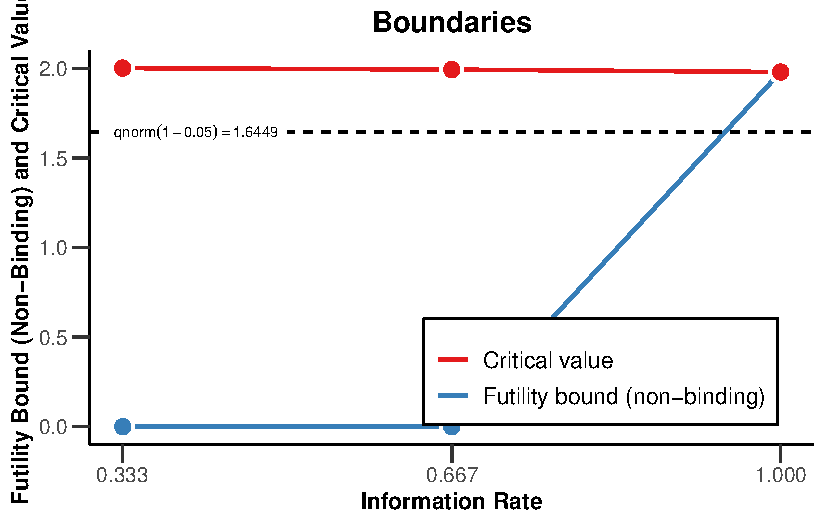
\includegraphics[width=1\textwidth,height=\textheight]{10-sequential_files/figure-pdf/fig-futility1-1.pdf}

}

\caption{\label{fig-futility1}Pocock类型用于拒绝\(H_0\)的边界(红线)以及当观察到的效应处于相反方向时用于无效停止的边界(蓝线)。}

\end{figure}

手动指定无效界线并不理想,因为我们有可能因为无法拒绝\(H_0\)而停止数据收集,出现二类错误的概率很高。更好的做法是通过直接控制数据的二类错误来设置无效界限。就像我们在中期分析中分配我们的一类错误率一样,我们可以在不同的观察(look)中分配我们的二类错误率,当我们不能以期望的二类错误率拒绝目标效应值时,可以决定停止无效性。

当一项研究被设计成使无效假设的显著性检验有90\%的效力来检测\emph{d}=0.5的效应时,10\%的情况\(H_0\)不会被拒绝,而它应该被拒绝。在这10\%的情况下,我们犯了二类错误,即虽然结论是不存在0.5的效应,而实际上,存在\emph{d}=0.5(或更大)的效应。在针对最小效应量\emph{d}=0.5的等效性实验中,当现实中存在\emph{d}=0.5(或更大)的效应时,得出0.5或更大的效应不存在的结论被称为一类错误。我们错误地得出了效应实际上等于零的结论。因此,当\(H_0\)为d=0,\(H_1\)=d=0.5时,在NHST中属于二类错误,而在\(H_0\)为d=0.5,\(H_1\)为d=0
的等价性检验中属于一类错误 (Jennison \& Turnbull,
2000)。因此,控制序列设计中的二类错误可以被看作是控制等效检验的一类错误,以对抗研究中的效应值。如果我们设计的研究有5\%的一类错误率和同样低的二类错误率(如5\%,或95\%的检验效力),那么该研究就是对存在或不存在目标效应的一种信息性检验。

如果真实效应值为(接近)0,则因无效而停止的序列设计比不因无效而停止的设计更有效。添加基于beta支出函数的无效边界会降低检验效力,这需要通过增加样本量来补偿,但这可以通过更早地因无效而停止研究这一事实来补偿,这可以使设计更有效率。当无法指定最小的目标效应值时,研究人员可能不希望将无效停止纳入研究设计。要控制观察的二类错误率,需要选择\textbf{beta
支出函数}(beta-spending
function),例如Pocock类型的beta支出函数、O'Brien-Fleming类型的beta支出函数或用户定义的
beta支出函数。例如,通过\emph{typeBetaSpending =
``bsP''}添加一个Pocock类型的beta支出函数。beta支出函数不需要与alpha支出函数相同。在\texttt{rpact}中,只能选择
beta支出函数进行定向(单侧)检验。毕竟,研究者可以考虑在两个方向上支持其假设的效应,而在相反方向上的效应作为拒绝备择假设的理由。

\begin{Shaded}
\begin{Highlighting}[]
\NormalTok{design }\OtherTok{\textless{}{-}} \FunctionTok{getDesignGroupSequential}\NormalTok{(}
  \AttributeTok{kMax =} \DecValTok{2}\NormalTok{,}
  \AttributeTok{typeOfDesign =} \StringTok{"asP"}\NormalTok{,}
  \AttributeTok{sided =} \DecValTok{1}\NormalTok{,}
  \AttributeTok{alpha =} \FloatTok{0.05}\NormalTok{,}
  \AttributeTok{beta =} \FloatTok{0.1}\NormalTok{,}
  \AttributeTok{typeBetaSpending =} \StringTok{"bsP"}\NormalTok{,}
  \AttributeTok{bindingFutility =} \ConstantTok{FALSE}
\NormalTok{  )}

\FunctionTok{plot}\NormalTok{(design)}
\end{Highlighting}
\end{Shaded}

\begin{figure}[H]

{\centering 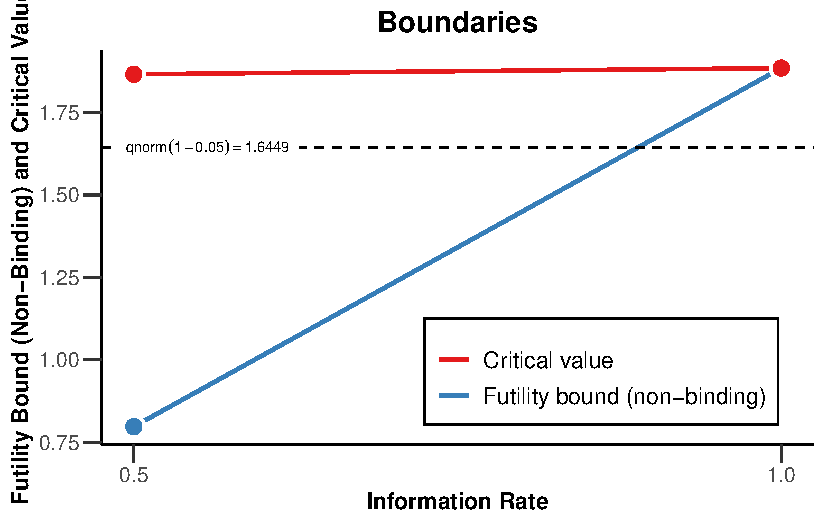
\includegraphics[width=1\textwidth,height=\textheight]{10-sequential_files/figure-pdf/fig-futility2-1.pdf}

}

\caption{\label{fig-futility2}3次观察的Pocock型边界看起来因拒绝\(H_0\)(红线)时停止,或者根据Pocock型beta
支出函数因无效而停止(蓝线)。}

\end{figure}

使用beta-spending函数,\(H_1\)下的预期被试数量将会增加,因此如果备择假设为真,设计一项能够因无效而停止的研究是有代价的。但是,\(H_0\)有可能为真,当它为真时,无效停止会减少预期的样本量。在图
Figure~\ref{fig-powerseq2}
中你可以看到,当真实效应量为0时,停止的概率(绿线)现在也很高,因为我们现在将因无效而停止,如果我们这样做,则预期样本量(蓝线)会比
Figure~\ref{fig-powerseq}
低。设计具有较高信息价值的研究,在最终分析时拒绝有意义的效应的存在是很重要的,但提前因无效而停止是否是你想在研究中建立的一个选项,这需要考虑无效假设为真的概率和样本量的增加(也许很小)。

\begin{figure}

{\centering 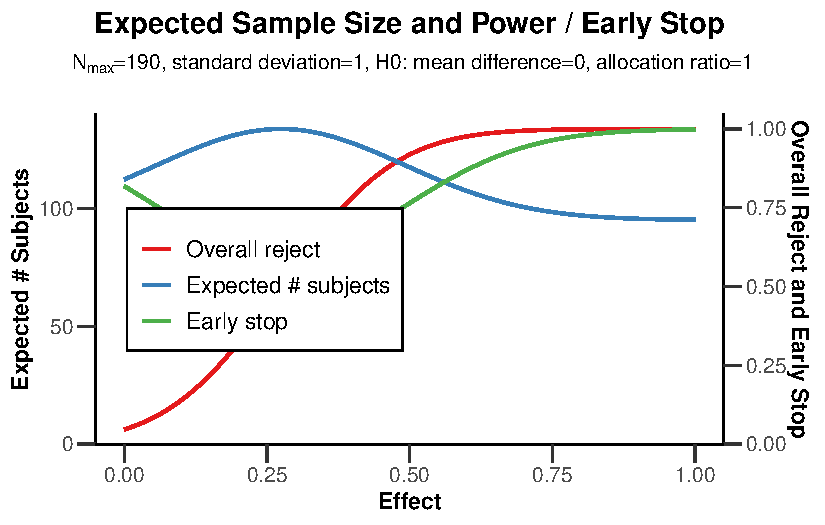
\includegraphics[width=1\textwidth,height=\textheight]{10-sequential_files/figure-pdf/fig-powerseq2-1.pdf}

}

\caption{\label{fig-powerseq2}具有两次观察的序列设计的功效曲线,因无效而停止。}

\end{figure}

\hypertarget{ux62a5ux544aux5e8fux5217ux5206ux6790ux7684ux7ed3ux679c}{%
\section{报告序列分析的结果}\label{ux62a5ux544aux5e8fux5217ux5206ux6790ux7684ux7ed3ux679c}}

组顺序设计的开发是为了使用Neyman-Pearson统计推断方法有效地检验假设,其目标是决定如何行动,同时控制长期的错误率。组序列设计的目标不是量化证据的强度,或提供效果大小的准确估计
(Proschan et al., 2006).
尽管如此,在得出假设是否可以被拒绝的结论后,研究人员在报告
结果时往往还想解释效果量的估计值。

在解释序列设计中观察到的效应值时的一个挑战是,每当研究被提前停止时,当\(H_0\)被拒绝时,数据分析就有可能被停止,因为由于随机变异,在中期分析时观察到了一个大的效应值。这意味着在这些中期分析中观察到的效应量高估了真正的效应量。
正如 Schönbrodt et al. (2017)
所展示的,对采用序列设计的研究进行元分析会得出准确的效应量,因为早期停止的研究样本量较小,权重较低,这被那些达到最后观察的序列研究中较小的效应值估计值所补偿,因为其样本量较大,权重较高。然而,研究人员可能希望在进行元分析之前解释单个研究的效应值,在这种情况下,报告校正后的效应值估计值可能是有所帮助的。尽管序列分析软件只允许人们计算某些统计检验的校正后(adjusted)的效应值的估计值,但我们建议在可能的情况下同时报告校正后的效应值,并始终为未来的元分析报告未经校正的效应值的估计值。

在报告\emph{p}值和置信区间时,也会出现类似的问题。当使用序列设计时,当\(H_0\)为真时,不考虑研究设计序列性的
\emph{p}值分布不再均匀。假设\(H_0\)为真,\emph{p}值是观察到的结果至少与观察到的结果一样极端的概率。确定\emph{至少一样极端}(at
least as extreme)意味着序列设计不再简单 (T. D. Cook,
2002)。为确定''至少同样极端''的含义,最常用的流程是根据就停止研究的观察来排列一系列序列分析的结果,当不同的研究同时停止时,早期停止的研究比后期停止的研究更极端,\emph{Z}值更高的研究更极端
(Proschan et al., 2006)。这被称为\emph{分阶段排序}(\emph{stagewise
ordering)},即与研究后期的拒绝相比,将早期的拒绝视为反对\(H_0\)的更有力证据
(Wassmer \& Brannath,
2016)。鉴于\emph{p}值和置信区间之间的直接关系,研究者也开发了序列设计的置信区间。

然而,报告校正后的\emph{p}值和置信区间可能会受到批评。在序列设计之后,基于Neyman-Pearson
的框架,得出以下结论是正确的解释:
\(H_0\)被拒绝,备择假设被拒绝,或者结果不确定。在序列设计之后报告校正后的\emph{p}值的原因是让读者将其解释为证据的一种衡量标准。Dupont
(1983)
为质疑校正后的\emph{p}值能否有效衡量证据强度提供了很好的论据。此外,对Neyman-Pearson统计推断方法的严格解释也为反对将\emph{p}值解释为证据度量提供了论据
(Lakens,
2022)。因此,如果研究人员有兴趣传达\(H_0\)数据中相对于备择假设的证据,建议报告可能性或贝叶斯系数,研究者可以在数据收集完成后报告和解释这些数据。报告与α水平有关的未经调整的p值,可以传达拒绝假设的依据,尽管这对于研究人员执行基于\emph{p}值的元分析(例如,\emph{p}曲线或\emph{z}曲线分析,如\protect\hyperlink{bias}{bias
detection}一章中所解释的),序列的\emph{p}值是连续可能很重要。校正后的置信区间是评估观察到的效应估计值相对于其在中期或最终观察得到的观察数据的变异性的有效工具。请注意,校正后的参数估计值只在统计软件中适用于药物试验中少数常用的设计,如组间平均差值的比较,或生存分析(survival
analysis)。

下面,我们看到与我们开始时一样的序列设计,有两次观察和一个Pocock类型的alpha支出函数。在完成每组95个参与者的预计样本量的研究后(我们在一次观察时收集48个参与者,在第二次观察时收集其余47个参与者),我们现在可以使用函数\texttt{getDataset}输入观察数据。输入每个阶段的平均值和标准差,所以在第二次观察时,只用每组后95名的参与者的数据来计算平均值(1.51
和 1.01)和标准差(1.03 和 0.96)。

\begin{Shaded}
\begin{Highlighting}[]
\NormalTok{design }\OtherTok{\textless{}{-}} \FunctionTok{getDesignGroupSequential}\NormalTok{(}
  \AttributeTok{kMax =} \DecValTok{2}\NormalTok{,}
  \AttributeTok{typeOfDesign =} \StringTok{"asP"}\NormalTok{,}
  \AttributeTok{sided =} \DecValTok{2}\NormalTok{,}
  \AttributeTok{alpha =} \FloatTok{0.05}\NormalTok{,}
  \AttributeTok{beta =} \FloatTok{0.1}
\NormalTok{)}

\NormalTok{dataMeans }\OtherTok{\textless{}{-}} \FunctionTok{getDataset}\NormalTok{(}
  \AttributeTok{n1 =} \FunctionTok{c}\NormalTok{(}\DecValTok{48}\NormalTok{, }\DecValTok{47}\NormalTok{), }
  \AttributeTok{n2 =} \FunctionTok{c}\NormalTok{(}\DecValTok{48}\NormalTok{, }\DecValTok{47}\NormalTok{), }
  \AttributeTok{means1 =} \FunctionTok{c}\NormalTok{(}\FloatTok{1.12}\NormalTok{, }\FloatTok{1.51}\NormalTok{), }\CommentTok{\# for directional test, means 1 \textgreater{} means 2}
  \AttributeTok{means2 =} \FunctionTok{c}\NormalTok{(}\FloatTok{1.03}\NormalTok{, }\FloatTok{1.01}\NormalTok{),}
  \AttributeTok{stDevs1 =} \FunctionTok{c}\NormalTok{(}\FloatTok{0.98}\NormalTok{, }\FloatTok{1.03}\NormalTok{), }
  \AttributeTok{stDevs2 =} \FunctionTok{c}\NormalTok{(}\FloatTok{1.06}\NormalTok{, }\FloatTok{0.96}\NormalTok{)}
\NormalTok{  )}

\NormalTok{res }\OtherTok{\textless{}{-}} \FunctionTok{getAnalysisResults}\NormalTok{(}
\NormalTok{  design, }
  \AttributeTok{equalVariances =} \ConstantTok{TRUE}\NormalTok{,}
  \AttributeTok{dataInput =}\NormalTok{ dataMeans}
\NormalTok{  )}

\NormalTok{res}
\end{Highlighting}
\end{Shaded}

\begin{verbatim}
[PROGRESS] Stage results calculated [0.0449 secs] 
[PROGRESS] Conditional power calculated [0.0997 secs] 
[PROGRESS] Conditional rejection probabilities (CRP) calculated [0.0018 secs] 
[PROGRESS] Repeated confidence interval of stage 1 calculated [0.8473 secs] 
[PROGRESS] Repeated confidence interval of stage 2 calculated [0.7409 secs] 
[PROGRESS] Repeated confidence interval calculated [1.59 secs] 
[PROGRESS] Repeated p-values of stage 1 calculated [0.3088 secs] 
[PROGRESS] Repeated p-values of stage 2 calculated [0.4101 secs] 
[PROGRESS] Repeated p-values calculated [0.7204 secs] 
[PROGRESS] Final p-value calculated [0.0025 secs] 
[PROGRESS] Final confidence interval calculated [0.1214 secs] 
\end{verbatim}

\hypertarget{analysis-results-means-of-2-groups-group-sequential-design}{%
\section{Analysis results (means of 2 groups, group sequential
design)}\label{analysis-results-means-of-2-groups-group-sequential-design}}

\hypertarget{design-parameters-3}{%
\subsection{Design parameters}\label{design-parameters-3}}

\begin{itemize}
\tightlist
\item
  \emph{Information rates}: 0.500, 1.000
\item
  \emph{Critical values}: 2.157, 2.201
\item
  \emph{Futility bounds (non-binding)}: -Inf
\item
  \emph{Cumulative alpha spending}: 0.03101, 0.05000
\item
  \emph{Local one-sided significance levels}: 0.01550, 0.01387
\item
  \emph{Significance level}: 0.0500
\item
  \emph{Test}: two-sided
\end{itemize}

\hypertarget{default-parameters-4}{%
\subsection{Default parameters}\label{default-parameters-4}}

\begin{itemize}
\tightlist
\item
  \emph{Normal approximation}: FALSE
\item
  \emph{Direction upper}: TRUE
\item
  \emph{Theta H0}: 0
\item
  \emph{Equal variances}: TRUE
\end{itemize}

\hypertarget{stage-results}{%
\subsection{Stage results}\label{stage-results}}

\begin{itemize}
\tightlist
\item
  \emph{Cumulative effect sizes}: 0.0900, 0.2928
\item
  \emph{Cumulative (pooled) standard deviations}: 1.021, 1.013
\item
  \emph{Stage-wise test statistics}: 0.432, 2.435
\item
  \emph{Stage-wise p-values}: 0.333390, 0.008421
\item
  \emph{Overall test statistics}: 0.432, 1.993
\item
  \emph{Overall p-values}: 0.33339, 0.02384
\end{itemize}

\hypertarget{analysis-results}{%
\subsection{Analysis results}\label{analysis-results}}

\begin{itemize}
\tightlist
\item
  \emph{Assumed standard deviation}: 1.013
\item
  \emph{Actions}: continue, accept
\item
  \emph{Conditional rejection probability}: 0.007317, NA
\item
  \emph{Conditional power}: NA, NA
\item
  \emph{Repeated confidence intervals (lower)}: -0.36630, -0.03306
\item
  \emph{Repeated confidence intervals (upper)}: 0.5463, 0.6187
\item
  \emph{Repeated p-values}: \textgreater0.5, 0.08195
\item
  \emph{Final stage}: 2
\item
  \emph{Final p-value}: NA, 0.06662
\item
  \emph{Final CIs (lower)}: NA, -0.02007
\item
  \emph{Final CIs (upper)}: NA, 0.5734
\item
  \emph{Median unbiased estimate}: NA, 0.2814
\end{itemize}

想象一下,我们进行了一项研究,计划最多对数据进行两次等距观察。在该研究中,我们进行alpha为0.05的双侧检验了,使用Pocock类型的
alpha支出函数,并在最后观察时检验两个组之间的均值差异。基于具有两个等距观察的Pocock类型的alpha支出函数,双侧\emph{t}检验的alpha水平是
0.003051, 和
0.0490。因此,我们可以在两次观察后拒绝\(H_0\)。但我们也想报告一个效应值,并校正\emph{p}值和置信区间。

结果表明,第一次观察后的操作是继续收集数据,并且可以在第二次观察时拒绝\(H_0\)。``总体效应值''(Overall
effect
size)行提供了未校正的平均差异,最后观察是0.293。``无偏估计中位数''(Median
unbiased estimate)提供了校正后的更低的平均差异,``最终置信区间''(Final
confidence interval)提供了校正后的置信区间,并给出结果0.281, 95\% CI
{[}-0.02, 0.573{]}。

单侧检验的未校正 \emph{p} 值在Overall
\emph{p}-value''行中报告。我们双侧检验的实际 \emph{p}
值将是原来的两倍大,即0.6668, 0.0477。最终查看时校正后的 \emph{p}
值在''Final \emph{p}-value''行中提供,为0.06662。

\hypertarget{ux6d4bux8bd5ux4e00ux4e0bux4f60ux81eaux5df1}{%
\section{测试一下你自己}\label{ux6d4bux8bd5ux4e00ux4e0bux4f60ux81eaux5df1}}

\textbf{Q1}:序列分析可以提高你执行的研究的效率。对于研究人员仅在可以拒绝\(H_0\)时才停止的顺序设计(并且没有指定因无效而停止的规则),以下哪项陈述是正确的?

\begin{enumerate}
\def\labelenumi{\Alph{enumi})}
\tightlist
\item
  序列分析将减少你要进行的每项研究的样本量
\item
  序列分析将平均减少你将进行的研究的样本量
\item
  只要有真实的效应,序列分析将平均减少你将进行的研究的样本量(当没有规定因无效而停止的规则时)
\item
  序列分析平均需要与固定设计相同的样本量,但提供更多的灵活性
\end{enumerate}

\textbf{Q2}:序列分析和选择性停止之间的区别是什么?

\begin{enumerate}
\def\labelenumi{\Alph{enumi})}
\tightlist
\item
  唯一的区别是,顺序分析是透明的报告,而选择性停止通常不在论文中披露
\item
  在序列分析中,第一类错误率是可控的,而在选择性停止中,第一类错误率是膨胀的
\item
  在选择性停止中,只有当观察到一个重要的结果时才会终止数据收集,而在顺序分析中,当确定没有一个有意义的影响时,数据收集也可以停止
\item
  在序列分析中,不可能设计一个在每个参与者之后就分析数据的研究,而在选择性停止中可以这样做
\end{enumerate}

\textbf{Q3}:Pocock校正的定义特征是什么?

\begin{enumerate}
\def\labelenumi{\Alph{enumi})}
\tightlist
\item
  它对早期观察使用非常保守的alpha水平,最后观察的alpha水平接近固定设计中未调整的alpha水平
\item
  它在每次观察时使用相同的 alpha
  水平(或者在使用Pocock型的alpha支出函数时,在每次观察时几乎使用相同的alpha水平)
\item
  它在每次中期分析时使用临界值3,并在最后一次观察时使用剩余的一类错误率
\item
  它有一个可以选择的参数,以便在早期中期分析中更保守或更自由地使用一类错误率
\end{enumerate}

\textbf{Q4}:O'Brien-Fleming校正的一个优势是最后一次观察时的alpha水平接近alpha水平。为什么?

\begin{enumerate}
\def\labelenumi{\Alph{enumi})}
\tightlist
\item
  这意味着基于先验功效分析(取决于alpha水平)的样本量接近固定设计中的样本量,同时允许额外观察数据
\item
  这意味着与固定设计相比,一类错误率并没有膨胀一点点
\item
  这意味着与固定设计相比,一类错误率只是稍微保守一点
\item
  这意味着基于先验功效分析(取决于alpha水平)的样本量始终与固定设计中的样本量相同,同时允许额外观察数据
\end{enumerate}

\textbf{Q5}:研究人员使用顺序设计进行研究,观察数据5次,双侧测试所需的总alpha水平为0.05,并选择\textbf{Pocock校正}。在继续收集数据至第三次查看后,研究人员观察到\emph{p}值为0.011。哪个论述是对的?注意:请记住\texttt{rpact}返回单侧alpha水平。你可以通过替换0并指定
typeOfDesign 来使用以下代码:

\begin{Shaded}
\begin{Highlighting}[]
\NormalTok{design }\OtherTok{\textless{}{-}}\NormalTok{ rpact}\SpecialCharTok{::}\FunctionTok{getDesignGroupSequential}\NormalTok{(}
  \AttributeTok{kMax =} \DecValTok{0}\NormalTok{,}
  \AttributeTok{typeOfDesign =} \StringTok{""}\NormalTok{,}
  \AttributeTok{sided =} \DecValTok{0}\NormalTok{,}
  \AttributeTok{alpha =} \FloatTok{0.0}
\NormalTok{)}
\NormalTok{design}
\end{Highlighting}
\end{Shaded}

\begin{enumerate}
\def\labelenumi{\Alph{enumi})}
\tightlist
\item
  研究人员可以拒绝原假设并可以终止数据收集
\item
  研究人员未能拒绝原假设,需要继续收集数据
\end{enumerate}

\textbf{Q6}:研究人员使用序列设计进行研究,观察数据5次,所需的总体alpha水平为0.05,并选择\textbf{O'Brien-Fleming校正}。在继续收集数据至第三次观察后,研究人员观察到
\emph{p} 值为 0.011。哪个陈述是正确的(你可以使用与 Q5 相同的代码)?

\begin{enumerate}
\def\labelenumi{\Alph{enumi})}
\tightlist
\item
  研究人员可以拒绝原假设并可以终止数据收集
\item
  研究人员未能拒绝原假设,需要继续收集数据
\end{enumerate}

\textbf{Q7}:对于Q5中的设计(使用Pocock
校正),达到80\%功效所需的样本量是多少(默认值------你可以通过指定不同于
\texttt{beta\ =\ 0.2} 的值来更改默认值\texttt{getDesignGroupSequential}
函数),效应量为\emph{d} =
0.5(等于平均差为0.5,标准差为1)。你可以使用下面的代码。

\begin{Shaded}
\begin{Highlighting}[]
\NormalTok{power\_res }\OtherTok{\textless{}{-}}\NormalTok{ rpact}\SpecialCharTok{::}\FunctionTok{getSampleSizeMeans}\NormalTok{(}
  \AttributeTok{design =}\NormalTok{ design,}
  \AttributeTok{groups =} \DecValTok{2}\NormalTok{,}
  \AttributeTok{alternative =} \FloatTok{0.5}\NormalTok{, }
  \AttributeTok{stDev =} \DecValTok{1}\NormalTok{, }
  \AttributeTok{allocationRatioPlanned =} \DecValTok{1}\NormalTok{,}
  \AttributeTok{normalApproximation =} \ConstantTok{FALSE}\NormalTok{)}

\NormalTok{power\_res}
\end{Highlighting}
\end{Shaded}

\begin{enumerate}
\def\labelenumi{\Alph{enumi})}
\tightlist
\item
  64个(每个独立组 32 个)
\item
  128 (每个独立组 64)
\item
  154 (每个独立组 77)
\item
  158 (每个独立组 79)
\end{enumerate}

\textbf{Q8}:对于Q5中的设计,对于只有一次观察的固定设计,在 \emph{d} =
0.5 的效应量达到80\%功效所需的样本量是多少?首先更新设计(通过将
\texttt{kMax} 更改为 1),然后重新运行函数 \texttt{getSampleSizeMeans}。

\begin{enumerate}
\def\labelenumi{\Alph{enumi})}
\tightlist
\item
  64 个(每个独立组 32 个)
\item
  128 (每个独立组 64)
\item
  154 (每个独立组 77)
\item
  158 (每个独立组 79)
\end{enumerate}

我们看到由于选择了Pocock校正和观察数量(5,这导致最终观察的alpha水平较低),样本量增加了很多。序列设计的最大样本量与固定设计的样本量之比称为
\textbf{膨胀因子}(inflation
factor),它与效应量无关。虽然先验功效分析尚未针对所有类型的检验进行编程,但膨胀因子可用于计算相对于任何测试的固定设计所需的增加的观察次数。研究人员可以使用他们通常使用的工具对固定设计执行先验功效分析,并将观察总数乘以膨胀因子以确定序列设计所需的样本量。可以使用\texttt{getDesignCharacteristics}函数检索膨胀因子。

\textbf{Q9}:
首先,重新运行代码以创建序列设计,其中五次观察Q5中使用的数据。然后,运行下面的代码,找到膨胀因子。与固定设计相比,使用
Pocock校正的具有5个观察的序列设计的膨胀因子或所需的样本量增加是多少?请注意,在计算膨胀因子时,\texttt{rpact}不会将每组的观察次数四舍五入为整数。

\begin{Shaded}
\begin{Highlighting}[]
\NormalTok{rpact}\SpecialCharTok{::}\FunctionTok{getDesignCharacteristics}\NormalTok{(design)}
\end{Highlighting}
\end{Shaded}

\begin{enumerate}
\def\labelenumi{\Alph{enumi})}
\tightlist
\item
  膨胀因子是1
\item
  膨胀因子是1.0284
\item
  膨胀因子是1.2286
\item
  膨胀因子是1.2536
\end{enumerate}

\textbf{Q10}:
我们看到膨胀系数相当大,而且有一定的概率,我们将不得不收集比使用固定设计更多的观测值。重新运行Q7的代码(对于有5次观察的Pocock设计)。我们看到,平均而言,如果存在一个0.5的真实效应,我们将比固定设计更有效率。在\(H_1\)下,由\texttt{rpact}提供的预期被试数量是多少?

\begin{enumerate}
\def\labelenumi{\Alph{enumi})}
\tightlist
\item
  101.9
\item
  104.3
\item
  125.3
\item
  152.8
\end{enumerate}

我们看到序列设计平均来说会比固定设计更有效率,但关于所使用的具体序列设计之间的权衡,以及可能的好处是否值得收集额外数据的风险,必须根据具体情况来决定。

\textbf{Q11}:
首先,重新运行代码,创建一个顺序设计,对Q6中使用的数据进行5次观察(因此使用O'Brien-Fleming校正)。然后,运行下面的代码,找出这个设计的膨胀系数。什么膨胀系数?

\begin{enumerate}
\def\labelenumi{\Alph{enumi})}
\tightlist
\item
  膨胀系数是1
\item
  膨胀系数是1.0284
\item
  膨胀系数是1.2286
\item
  膨胀系数是1.2536
\end{enumerate}

\textbf{Q12}:
也可以因无用而停止(或拒绝存在感兴趣的特定效应)。研究者应该在有约束力和无约束力的beta支出函数之间做出决定,但他们不需要在有约束力和无约束力的alpha支出函数之间做出决定。如果研究者在中期分析时观察到一个有统计学意义的结果,但决定不停止数据收集,而是继续收集数据(例如,为了获得更精确的效应量估计),会有什么后果?

\begin{enumerate}
\def\labelenumi{\Alph{enumi})}
\tightlist
\item
  第一类错误率会膨胀,第二类错误率也会膨胀
\item
  第一类错误率会膨胀,而第二类错误率不会膨胀
\item
  第一类错误率不会膨胀,第二类错误率会膨胀
\item
  第一类错误率不会膨胀,第二类错误率也不会膨胀
\end{enumerate}

\textbf{Q13}:
在下图中,您可以看到序列设计的\emph{t}分数边界停止拒绝\(H_0\)(红线)和拒绝\(H_1\)(蓝线)。在第二次临观察时,你执行了一项检验,观察到\emph{t}值为2。您会做出哪个决定?

\begin{figure}

{\centering 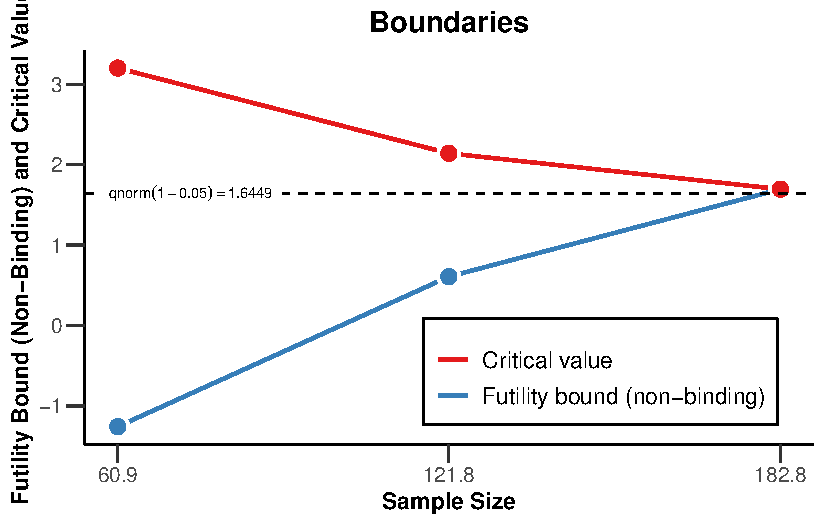
\includegraphics[width=1\textwidth,height=\textheight]{10-sequential_files/figure-pdf/fig-futilityq13-1.pdf}

}

\caption{\label{fig-futilityq13}3次观察O'Brien-Fleming类型边界拒绝
\(H_0\)(红线)时停止或因5\%的一类和二类错误而无效停止(蓝线)的例子}

\end{figure}

\begin{enumerate}
\def\labelenumi{\Alph{enumi})}
\tightlist
\item
  你可以拒绝\(H_0\)并停止数据收集
\item
  你可以拒绝\(H_1\)并停止数据收集
\item
  你拒绝\(H_0\)和\(H_1\)并停止数据收集
\item
  你未能同时拒绝\(H_0\)和\(H_1\)并继续收集数据
\end{enumerate}

\hypertarget{ux5f00ux653eux6027ux95eeux9898-2}{%
\subsection{10.9.1 开放性问题}\label{ux5f00ux653eux6027ux95eeux9898-2}}

\begin{enumerate}
\def\labelenumi{\arabic{enumi}.}
\item
  序列分析和选择性停止有什么区别?
\item
  与固定设计相比,使用序列设计的可能好处是什么?
\item
  因无效而停止数据收集是什么意思?
\item
  Pocock和 O'Brien-Fleming方法在观察上指出alpha的理念有何不同?
\item
  使用O'Brien-Fleming校正时最终观察的alpha水平接近未校正的alpha水平有什么优势?
\item
  Pocock和O'Brien-Fleming校正与Lan和DeMets开发的相应Pocock和O'Brien-Fleming
  alpha支出函数有什么区别?
\item
  即使序列设计的最大样本量略大于固定设计的样本量,为什么序列设计仍然可以更有效?
\item
  什么时候合并无效停止规则会提高顺序设计的效率?
\item
  平均而言,在序列设计中提前停止对效应量估计有何影响?报告时不校正效应量估计的理由是什么?
\end{enumerate}

\bookmarksetup{startatroot}

\hypertarget{sec-bias}{%
\chapter{偏倚检测}\label{sec-bias}}

在整个研究过程中都可能会出现偏差。察觉并预防偏差的出现将会有很大的帮助。一些研究者建议对科学文献中的任何结论都持怀疑态度。例如,科学哲学家Deborah~Mayo(2018)写道:``面对最新的统计学新闻时,你的第一个问题应该是:这些结果是由于选择性报告、选择性挑选或者其他类似伎俩导致的吗?''。如果你在下一次参加的科学会议上问这个问题,可能会让自己不那么受欢迎,但忽视研究者或多或少有意地在他们的结论中引入偏差这一事实是非常幼稚的。

在引入偏差到科学研究的行为中,最极端的形式就是\textbf{研究不当行为},包括伪造数据或结果、更改或剔除数据或结果,使得研究记录不能准确反映研究发现。例如,\href{https://en.wikipedia.org/wiki/Andrew_Wakefield}{Andrew
Wakefield}在1998年撰写了一篇造假文章,声称麻疹、流行性腮腺炎和风疹(MMR)疫苗与自闭症有关。这篇文章在破坏了一些公众对疫苗的信任后,才终于在2010年被撤销。另一个例子来自心理学领域,\href{https://en.wikipedia.org/wiki/James_Vicary}{James~Vicary}进行的一项关于潜意识启示的研究。他声称,在电影院屏幕上闪现低于意识阈限的词语''吃爆米花''和''喝可乐'',爆米花和可乐的销售额分别增长了57.5\%、18.1\%.~然而,人们后来发现Vicary很可能进行了学术欺诈,因为没有任何证据表明确实进行过这样一项研究(S.
Rogers,
1992)。Retraction-Watch网站维护着一个\href{http://retractiondatabase.org}{数据库},跟踪记录了科学论文被撤销的原因,包括数据造假。虽然实际中数据造假的发生频率未知,但正如\protect\hyperlink{integrity}{研究诚信}章节中所讨论的那样,我们应该可以预计至少有一小部分科学家对数据和结果进行过一次以上的捏造和篡改。

\begin{figure}

{\centering 
\includegraphics[width=1\textwidth,height=\textheight]{images/dropout_outlier.png}

}

\caption{\label{fig-outliers}《The~Dropout》中的一幕,讲述了Theranos公司虚假宣传拥有可以使用极少量血液进行血液检测的设备。在这一幕中,两名举报者在与他们的上司进行对峙,起因是他们被强迫删除不符合预期结果的数据。}

\end{figure}

另一类错误是统计报告错误,包括报告错误的自由度、将p=0.056报告为p\textless0.05等(Nuijten
et al.,
2015)。虽然我们应该尽力避免错误,但每个人都会犯错,而随着数据和代码共享变得越来越普遍,能够更容易地检测出其他研究人员工作中的错误。正如Dorothy~Bishop(2018)所写的:``随着开放科学越来越成为常态,我们将发现每个人会犯错误。科学家的声誉将不取决于他们的研究中是否存在缺陷,而是取决于在发现这些缺陷时他们如何回应。

\href{http://statcheck.io/}{Statcheck}是一款自动从文章中提取统计数据并重新计算其p值的软件,统计数据需要按照美国心理学协会(APA)的指导方针报告。它会检查报告的统计数据内部是否一致:在给定的检验统计数据和自由度下,报告的p值是否准确?如果准确,那么犯错的可能性就较小(但这并不适用于逻辑错误!),如果不准确,你应该检查统计检验中的所有信息是否准确。Statcheck不是完美的,它会导致第一类错误,即当实际上没有错误时,它将某些内容标记为错误,但它是一个易于使用的工具,可以在投稿之前用来检查文章。

有些数据的不一致性不太容易自动检测,但可以手动识别。例如,N. J. L. Brown
\& Heathers (2017)
表明,许多论文报告的平均值在样本量给定的情况下不可能出现(称为\href{http://nickbrown.fr/GRIM}{\emph{GRIM}}\href{http://nickbrown.fr/GRIM}{~test})。例如,Matti~Heino在一篇博客文章\href{https://mattiheino.com/2016/11/13/legacy-of-psychology/}{blog~post}中注意到,Festinger和Carlsmith的经典研究表格中报告的三个平均值在数学上是不可能的。对于每个条件20个观测值和-5到5的标度,所有平均值应该以1/20的倍数或0.05结尾。以X.X8或X.X2结尾的三个平均值与报告的样本量和标度不一致。当然,这种不一致性可能是由于未报告某些问题的数据缺失引起的,但GRIM测试也已被用于揭示科学不端行为\href{https://en.wikipedia.org/wiki/GRIM_test}{scientific~misconduct}。

\begin{figure}

{\centering \includegraphics[width=1\textwidth,height=\textheight]{images/festinger_carlsmith.png}

}

\caption{\label{fig-festinger}1959年Festinger和Carlsmith所作报告中主要结果的表格截图。}

\end{figure}

\hypertarget{publicationbias}{%
\section{出版偏见}\label{publicationbias}}

出版偏见是科学面临的最大挑战之一。\textbf{出版偏见}指有选择地提交和出版科学研究,通常基于结果是否有''统计显著''。科学文献被这些统计显著的结果所主导。同时,我们知道,研究人员进行的许多研究并没有产生显著的结果。当科学家们只能获得显著的结果,而不能获得所有的结果时,他们就缺乏对某一假设的证据的完整概述。在极端情况下,选择性报告会导致这样一种情况:在已发表的文献中,有数百个统计显著的结果,但因为有更多非显著的研究没有被分享,学术研究没有真正的效果。这就是所谓的\textbf{文件抽屉问题},即非显著结果被藏在文件抽屉里(或者现在是电脑上的文件夹),不为科学界所了解。每个科学家都应该努力解决出版偏见,因为只要科学家不分享他们的所有结果,就很难了解什么是可能的事实,而且正如Greenwald(1975)所指出的,这是一种违反道德的行为。

\begin{figure}

{\centering \includegraphics[width=1\textwidth,height=\textheight]{images/greenwald.png}

}

\caption{\label{fig-greenwald}Greenwald,A.G.(1975)最后一句话的截图,这篇文章指出对无效假设偏见的后果。Psychological\&Bulletin,
82(1), 1--20.}

\end{figure}

只有将你的所有研究成果提供给科学家同行,无论主要假设检验的\emph{p}值是多少,才能解决出版偏差的问题。注册报告是消除出版偏见的一种方式,因为这种类型的科学文章在收集数据之前,会根据介绍、方法和统计分析计划进行审查(Chambers
\& Tzavella, 2022; Nosek \& Lakens,
2014)。经过该领域专家的同行评审,他们可能会对实验设计和数据分析方法提出改进意见。文章可以获准
``原则上接收'',这意味着只要遵循研究计划,无论结果如何,文章就会被发表。这应该有利于非显著性结果的发表,如图所示
Figure~\ref{fig-scheel}
,对首次发表的心理学注册报告的分析显示,71篇文章中的31篇(44\%)观察到了显著结果,相比之下,同期发表的152篇标准科学文章中的则有146篇(96\%)观察到了显著结果(Scheel,
Schijen, et al., 2021) 。

\begin{figure}

{\centering \includegraphics[width=0.75\textwidth,height=\textheight]{images/scheel.png}

}

\caption{\label{fig-scheel}标准报告和注册报告的显著结果率,误差条表示95\%置信区间。}

\end{figure}

在过去,注册报告并不存在,科学家也不会分享所有的结果(Franco et al.,
2014; Greenwald, 1975; Sterling,
1959),因此,我们必须努力检测出版偏差对我们准确评估文献能力的影响程度。元分析应该始终仔细检查出版偏差对元分析效应量估计的影响--尽管在1990年至2017年间发表在Psychological
Bulletin上的元分析中,估计只有57\%文章说他们评估了出版偏差(Polanin et
al.,
2020)。最近发表在教育研究上的元分析中,82\%使用了偏差检测测试,但所使用的方法通常与最先进的方法相差甚远(Ropovik
et al.,
2021)。目前已经开发了几种检验出版偏差的技术,但这仍然是一个非常活跃的研究领域。所有的技术都是基于特定的假设,你在应用检验测试之前应该考虑这些假设(Carter
et al.,
2019)。目前并没有''妙方'':这些技术都不能纠正出版偏差。它们都不能肯定地告诉你修正了出版偏差后真正的元分析效应量是多少。这些方法能做到最好的事情就是在特定条件下检测由特定机制引起的出版偏差。出版偏差可以被检测出来,但它不能被修正。

在似然一章中,我们看到混合结果是可以预期的,而且可以成为替代性假设的有力证据。不仅混合结果是可以预期的,而且可以专门观察到统计显著的结果,尤其是在统计检验力较低的情况下,这非常令人惊讶。以通常使用的80\%的统计检验力下限,我们可以预期在有真实效果的情况下,五项研究中会有一项是不显著的结果。一些研究人员指出,在一组研究中,\emph{不}发现混合结果非常不可能(换言之,``好得不真实'')(Francis,
2014; Schimmack, 2012)
。我们对真实的研究模式没有很好的感受,因为我们持续接触到的科学文献并不反映现实情况。科学文献中几乎所有的多项研究论文都只呈现统计显著的结果,尽管这不可能。

我们开发了计算二项式概率的\href{http://shiny.ieis.tue.nl/mixed_results_likelihood/}{在线Shiny应用程序}。如果你滚动到页面底部,在''二项式概率''中找到''多项显著性发现'',给定一个关于检验力的特定假设,应用程序便可显示概率。Francis
(2014) 使用这些二项式概率来计算2009年至2012年期间发表在Psychological
Science杂志上44篇包含四个或更多研究的文章的过度显著结果(Ioannidis \&
Trikalinos,
2007)。他发现,对于这些文章中的36篇,考虑到根据观察到的效应量计算的平均检验力,观察到四个显著性结果的可能性小于10\%。鉴于他选择的α水平为0.10,这个二项式概率是一个假设检验,并允许声称(在10\%的α水平下):只要统计显著的结果数量的二项式概率低于10\%,数据是出乎意料的,由此我们可以拒绝''这是一组没有引入偏见的研究''这一假设。换句话说,不太可能观察到这么多显著的结果,这表明出版偏差或其他选择效应在这些文章中发挥了作用。

这44篇文章中,有一篇由我自己共同撰写(Jostmann et al.,
2009)。那时,我对统计检验力和出版偏见知之甚少,被指责为进行不正当学术行为令我倍感压力。然而,这些指责是正确的--我们有选择地报告了结果,有选择地报告了有效的分析。由于几乎没有接受过这方面的培训,我们对自己进行了教育,并将一项未发表的研究上传到网站psychfiledrawer.org(该网站已不存在),以分享我们的''文件抽屉''。若干年后,当Many
Labs
3将我们发表的一项研究纳入他们复制的研究集时,我们提供了帮助(Ebersole et
al.,
2016)。当观察到一个无效的结果时,我们写道:``我们不得不得出结论,实际上没有可靠的证据证明这种效应''(Jostmann
et al., 2016)。我希望这些教育材料能够避免其他人像我们一样出丑。

\hypertarget{ux5143ux5206ux6790ux4e2dux7684ux504fux5deeux68c0ux6d4b}{%
\section{元分析中的偏差检测}\label{ux5143ux5206ux6790ux4e2dux7684ux504fux5deeux68c0ux6d4b}}

检测发表偏差的新方法不断被开发出来,而旧的方法则变得过时(尽管你仍然可以看到它们出现在元分析中)。一种过时的方法被称为\textbf{故障安全N(fail-safe
N)}。其想法是计算在观察到的元分析效应量估计值不再与0有统计学差异之前,在文件抽屉中需要有多少个不显着的结果。这种方法已\href{https://handbook-5-1.cochrane.org/chapter_10/10_4_4_3_fail_safe_n.htm}{不再被推荐},Becker(2005)写道:``鉴于现在有其他处理发表偏倚的方法,应该放弃故障安全N方法,而采用其他更富有信息量的分析方法。目前,故障安全N的唯一用途是作为一种工具来识别那些不是最先进的元分析。

在我们解释第二种方法(修剪和填充,Trim-and-Fill)之前,有必要解释一下可视化元分析的一种常见方法,即\textbf{漏斗图}。在漏斗图中,X轴用于绘制每个研究的效应量,Y轴用于绘制每个效应量的''精确度''(通常是每个效应量估计的标准误差)。一项研究中的观察数越多,效应量的估计就越精确,标准误差就越小,因此该研究在漏斗图中的位置就越高。一个无限精确的研究(标准误差为0)将位于y轴的顶端。

下面的代码模拟了\texttt{nsims}研究的荟萃分析,并存储了检查偏差检测所需的所有结果。在代码的第一部分中,模拟了所需方向上具有统计显着性的结果,在第二部分中生成了空结果。
如\texttt{pub.bias}所示,该代码会生成一定比例的重要结果------当设置为
11时,所有结果都是重要的。 在下面的代码中,\texttt{pub.bias}设置为
0.05。
因为模拟中没有真正的效果(\texttt{m1}和\texttt{m2}相等,所以组间没有差异),唯一应该预期的显着结果是
5\% 的误报。最后,执行元分析,输出结果,并创建漏斗图。

\begin{Shaded}
\begin{Highlighting}[]
\FunctionTok{library}\NormalTok{(metafor)}
\FunctionTok{library}\NormalTok{(truncnorm)}

\NormalTok{nsims }\OtherTok{\textless{}{-}} \DecValTok{100} \CommentTok{\# number of simulated experiments}
\NormalTok{pub.bias }\OtherTok{\textless{}{-}} \FloatTok{0.05} \CommentTok{\# set percentage of significant results in the literature}

\NormalTok{m1 }\OtherTok{\textless{}{-}} \DecValTok{0} \CommentTok{\# too large effects will make non{-}significant results extremely rare}
\NormalTok{sd1 }\OtherTok{\textless{}{-}} \DecValTok{1}
\NormalTok{m2 }\OtherTok{\textless{}{-}} \DecValTok{0}
\NormalTok{sd2 }\OtherTok{\textless{}{-}} \DecValTok{1}
\NormalTok{metadata.sig }\OtherTok{\textless{}{-}} \FunctionTok{data.frame}\NormalTok{(}\AttributeTok{m1 =} \ConstantTok{NA}\NormalTok{, }\AttributeTok{m2 =} \ConstantTok{NA}\NormalTok{, }\AttributeTok{sd1 =} \ConstantTok{NA}\NormalTok{, }\AttributeTok{sd2 =} \ConstantTok{NA}\NormalTok{, }
                           \AttributeTok{n1 =} \ConstantTok{NA}\NormalTok{, }\AttributeTok{n2 =} \ConstantTok{NA}\NormalTok{, }\AttributeTok{pvalues =} \ConstantTok{NA}\NormalTok{, }\AttributeTok{pcurve =} \ConstantTok{NA}\NormalTok{)}
\NormalTok{metadata.nonsig }\OtherTok{\textless{}{-}} \FunctionTok{data.frame}\NormalTok{(}\AttributeTok{m1 =} \ConstantTok{NA}\NormalTok{, }\AttributeTok{m2 =} \ConstantTok{NA}\NormalTok{, }\AttributeTok{sd1 =} \ConstantTok{NA}\NormalTok{, }\AttributeTok{sd2 =} \ConstantTok{NA}\NormalTok{, }
                              \AttributeTok{n1 =} \ConstantTok{NA}\NormalTok{, }\AttributeTok{n2 =} \ConstantTok{NA}\NormalTok{, }\AttributeTok{pvalues =} \ConstantTok{NA}\NormalTok{, }\AttributeTok{pcurve =} \ConstantTok{NA}\NormalTok{)}

\CommentTok{\# simulate significant effects in the expected direction}
\ControlFlowTok{if}\NormalTok{(pub.bias }\SpecialCharTok{\textgreater{}} \DecValTok{0}\NormalTok{)\{}
\ControlFlowTok{for}\NormalTok{ (i }\ControlFlowTok{in} \DecValTok{1}\SpecialCharTok{:}\NormalTok{nsims}\SpecialCharTok{*}\NormalTok{pub.bias) \{ }\CommentTok{\# for each simulated experiment}
\NormalTok{  p }\OtherTok{\textless{}{-}} \DecValTok{1} \CommentTok{\# reset p to 1}
\NormalTok{  n }\OtherTok{\textless{}{-}} \FunctionTok{round}\NormalTok{(truncnorm}\SpecialCharTok{::}\FunctionTok{rtruncnorm}\NormalTok{(}\DecValTok{1}\NormalTok{, }\DecValTok{20}\NormalTok{, }\DecValTok{1000}\NormalTok{, }\DecValTok{100}\NormalTok{, }\DecValTok{100}\NormalTok{)) }\CommentTok{\# n based on truncated normal}
  \ControlFlowTok{while}\NormalTok{ (p }\SpecialCharTok{\textgreater{}} \FloatTok{0.025}\NormalTok{) \{ }\CommentTok{\# continue simulating as along as p is not significant}
\NormalTok{    x }\OtherTok{\textless{}{-}} \FunctionTok{rnorm}\NormalTok{(}\AttributeTok{n =}\NormalTok{ n, }\AttributeTok{mean =}\NormalTok{ m1, }\AttributeTok{sd =}\NormalTok{ sd1) }
\NormalTok{    y }\OtherTok{\textless{}{-}} \FunctionTok{rnorm}\NormalTok{(}\AttributeTok{n =}\NormalTok{ n, }\AttributeTok{mean =}\NormalTok{ m2, }\AttributeTok{sd =}\NormalTok{ sd2) }
\NormalTok{    p }\OtherTok{\textless{}{-}} \FunctionTok{t.test}\NormalTok{(x, y, }\AttributeTok{alternative =} \StringTok{"greater"}\NormalTok{, }\AttributeTok{var.equal =} \ConstantTok{TRUE}\NormalTok{)}\SpecialCharTok{$}\NormalTok{p.value}
\NormalTok{  \}}
\NormalTok{  metadata.sig[i, }\DecValTok{1}\NormalTok{] }\OtherTok{\textless{}{-}} \FunctionTok{mean}\NormalTok{(x)}
\NormalTok{  metadata.sig[i, }\DecValTok{2}\NormalTok{] }\OtherTok{\textless{}{-}} \FunctionTok{mean}\NormalTok{(y)}
\NormalTok{  metadata.sig[i, }\DecValTok{3}\NormalTok{] }\OtherTok{\textless{}{-}} \FunctionTok{sd}\NormalTok{(x)}
\NormalTok{  metadata.sig[i, }\DecValTok{4}\NormalTok{] }\OtherTok{\textless{}{-}} \FunctionTok{sd}\NormalTok{(y)}
\NormalTok{  metadata.sig[i, }\DecValTok{5}\NormalTok{] }\OtherTok{\textless{}{-}}\NormalTok{ n}
\NormalTok{  metadata.sig[i, }\DecValTok{6}\NormalTok{] }\OtherTok{\textless{}{-}}\NormalTok{ n}
\NormalTok{  out }\OtherTok{\textless{}{-}} \FunctionTok{t.test}\NormalTok{(x, y, }\AttributeTok{var.equal =} \ConstantTok{TRUE}\NormalTok{)}
\NormalTok{  metadata.sig[i, }\DecValTok{7}\NormalTok{] }\OtherTok{\textless{}{-}}\NormalTok{ out}\SpecialCharTok{$}\NormalTok{p.value}
\NormalTok{  metadata.sig[i, }\DecValTok{8}\NormalTok{] }\OtherTok{\textless{}{-}} \FunctionTok{paste0}\NormalTok{(}\StringTok{"t("}\NormalTok{, out}\SpecialCharTok{$}\NormalTok{parameter, }\StringTok{")="}\NormalTok{, out}\SpecialCharTok{$}\NormalTok{statistic)}
\NormalTok{\}\}}

\CommentTok{\# simulate non{-}significant effects (two{-}sided)}
\ControlFlowTok{if}\NormalTok{(pub.bias }\SpecialCharTok{\textless{}} \DecValTok{1}\NormalTok{)\{}
\ControlFlowTok{for}\NormalTok{ (i }\ControlFlowTok{in} \DecValTok{1}\SpecialCharTok{:}\NormalTok{nsims}\SpecialCharTok{*}\NormalTok{(}\DecValTok{1}\SpecialCharTok{{-}}\NormalTok{pub.bias)) \{ }\CommentTok{\# for each simulated experiment}
\NormalTok{  p }\OtherTok{\textless{}{-}} \DecValTok{0} \CommentTok{\# reset p to 1}
\NormalTok{  n }\OtherTok{\textless{}{-}} \FunctionTok{round}\NormalTok{(truncnorm}\SpecialCharTok{::}\FunctionTok{rtruncnorm}\NormalTok{(}\DecValTok{1}\NormalTok{, }\DecValTok{20}\NormalTok{, }\DecValTok{1000}\NormalTok{, }\DecValTok{100}\NormalTok{, }\DecValTok{100}\NormalTok{))}
  \ControlFlowTok{while}\NormalTok{ (p }\SpecialCharTok{\textless{}} \FloatTok{0.05}\NormalTok{) \{ }\CommentTok{\# continue simulating as along as p is significant}
\NormalTok{    x }\OtherTok{\textless{}{-}} \FunctionTok{rnorm}\NormalTok{(}\AttributeTok{n =}\NormalTok{ n, }\AttributeTok{mean =}\NormalTok{ m1, }\AttributeTok{sd =}\NormalTok{ sd1) }\CommentTok{\# produce  simulated participants}
\NormalTok{    y }\OtherTok{\textless{}{-}} \FunctionTok{rnorm}\NormalTok{(}\AttributeTok{n =}\NormalTok{ n, }\AttributeTok{mean =}\NormalTok{ m2, }\AttributeTok{sd =}\NormalTok{ sd2) }\CommentTok{\# produce  simulated participants}
\NormalTok{    p }\OtherTok{\textless{}{-}} \FunctionTok{t.test}\NormalTok{(x, y, }\AttributeTok{var.equal =} \ConstantTok{TRUE}\NormalTok{)}\SpecialCharTok{$}\NormalTok{p.value}
\NormalTok{  \}}
\NormalTok{  metadata.nonsig[i, }\DecValTok{1}\NormalTok{] }\OtherTok{\textless{}{-}} \FunctionTok{mean}\NormalTok{(x)}
\NormalTok{  metadata.nonsig[i, }\DecValTok{2}\NormalTok{] }\OtherTok{\textless{}{-}} \FunctionTok{mean}\NormalTok{(y)}
\NormalTok{  metadata.nonsig[i, }\DecValTok{3}\NormalTok{] }\OtherTok{\textless{}{-}} \FunctionTok{sd}\NormalTok{(x)}
\NormalTok{  metadata.nonsig[i, }\DecValTok{4}\NormalTok{] }\OtherTok{\textless{}{-}} \FunctionTok{sd}\NormalTok{(y)}
\NormalTok{  metadata.nonsig[i, }\DecValTok{5}\NormalTok{] }\OtherTok{\textless{}{-}}\NormalTok{ n}
\NormalTok{  metadata.nonsig[i, }\DecValTok{6}\NormalTok{] }\OtherTok{\textless{}{-}}\NormalTok{ n}
\NormalTok{  out }\OtherTok{\textless{}{-}} \FunctionTok{t.test}\NormalTok{(x, y, }\AttributeTok{var.equal =} \ConstantTok{TRUE}\NormalTok{)}
\NormalTok{  metadata.nonsig[i, }\DecValTok{7}\NormalTok{] }\OtherTok{\textless{}{-}}\NormalTok{ out}\SpecialCharTok{$}\NormalTok{p.value}
\NormalTok{  metadata.nonsig[i, }\DecValTok{8}\NormalTok{] }\OtherTok{\textless{}{-}} \FunctionTok{paste0}\NormalTok{(}\StringTok{"t("}\NormalTok{, out}\SpecialCharTok{$}\NormalTok{parameter, }\StringTok{")="}\NormalTok{, out}\SpecialCharTok{$}\NormalTok{statistic)}
\NormalTok{\}\}}

\CommentTok{\# Combine significant and non{-}significant effects}
\NormalTok{metadata }\OtherTok{\textless{}{-}} \FunctionTok{rbind}\NormalTok{(metadata.nonsig, metadata.sig)}

\CommentTok{\# Use escalc to compute effect sizes}
\NormalTok{metadata }\OtherTok{\textless{}{-}} \FunctionTok{escalc}\NormalTok{(}\AttributeTok{n1i =}\NormalTok{ n1, }\AttributeTok{n2i =}\NormalTok{ n2, }\AttributeTok{m1i =}\NormalTok{ m1, }\AttributeTok{m2i =}\NormalTok{ m2, }\AttributeTok{sd1i =}\NormalTok{ sd1, }
  \AttributeTok{sd2i =}\NormalTok{ sd2, }\AttributeTok{measure =} \StringTok{"SMD"}\NormalTok{, }\AttributeTok{data =}\NormalTok{ metadata[}\FunctionTok{complete.cases}\NormalTok{(metadata),])}
\CommentTok{\# add se for PET{-}PEESE analysis}
\NormalTok{metadata}\SpecialCharTok{$}\NormalTok{sei }\OtherTok{\textless{}{-}} \FunctionTok{sqrt}\NormalTok{(metadata}\SpecialCharTok{$}\NormalTok{vi)}

\CommentTok{\#Perform meta{-}analysis}
\NormalTok{result }\OtherTok{\textless{}{-}}\NormalTok{ metafor}\SpecialCharTok{::}\FunctionTok{rma}\NormalTok{(yi, vi, }\AttributeTok{data =}\NormalTok{ metadata)}
\NormalTok{result}

\CommentTok{\# Print a Funnel Plot}
\NormalTok{metafor}\SpecialCharTok{::}\FunctionTok{funnel}\NormalTok{(result, }\AttributeTok{level =} \FloatTok{0.95}\NormalTok{, }\AttributeTok{refline =} \DecValTok{0}\NormalTok{)}
\FunctionTok{abline}\NormalTok{(}\AttributeTok{v =}\NormalTok{ result}\SpecialCharTok{$}\NormalTok{b[}\DecValTok{1}\NormalTok{], }\AttributeTok{lty =} \StringTok{"dashed"}\NormalTok{) }\CommentTok{\# vertical line at meta{-}analytic ES}
\FunctionTok{points}\NormalTok{(}\AttributeTok{x =}\NormalTok{ result}\SpecialCharTok{$}\NormalTok{b[}\DecValTok{1}\NormalTok{], }\AttributeTok{y =} \DecValTok{0}\NormalTok{, }\AttributeTok{cex =} \FloatTok{1.5}\NormalTok{, }\AttributeTok{pch =} \DecValTok{17}\NormalTok{) }\CommentTok{\# add point}
\end{Highlighting}
\end{Shaded}

让我们先看看无偏见的研究是什么样子的,运行代码,保持\texttt{pub.bias}在0.05,这样只有5\%的第一类错误进入科学文献。

\begin{verbatim}
Loading required package: Matrix
\end{verbatim}

\begin{verbatim}
Loading required package: metadat
\end{verbatim}

\begin{verbatim}
Loading required package: numDeriv
\end{verbatim}

\begin{verbatim}

Loading the 'metafor' package (version 4.4-0). For an
introduction to the package please type: help(metafor)
\end{verbatim}

\begin{verbatim}

Random-Effects Model (k = 100; tau^2 estimator: REML)

tau^2 (estimated amount of total heterogeneity): 0.0000 (SE = 0.0018)
tau (square root of estimated tau^2 value):      0.0006
I^2 (total heterogeneity / total variability):   0.00%
H^2 (total variability / sampling variability):  1.00

Test for Heterogeneity:
Q(df = 99) = 91.7310, p-val = 0.6851

Model Results:

estimate      se     zval    pval    ci.lb   ci.ub    
 -0.0021  0.0121  -0.1775  0.8591  -0.0258  0.0215    

---
Signif. codes:  0 '***' 0.001 '**' 0.01 '*' 0.05 '.' 0.1 ' ' 1
\end{verbatim}

当我们检查元分析的结果时,我们看到元分析中有100个研究(\texttt{k\ =\ 100}),并且没有统计意义上的异质性(\emph{p}
=
0.69,这并不令人惊讶,因为我们在编程时将模拟的真实效应量设定为0,并且没有效应量的异质性)。我们也得到了元的结果。元分析的估计值是\emph{d}=-0.002,非常接近于0(应该如此,因为真实的效应量确实是0)。这个估计值的标准误差是0.012。有了100项研究,我们就有了对真实效应量的非常准确的估计。对\emph{d}=0的检验的\emph{Z}值是-0.177,而这个检验的\emph{p}值是0.86。我们不能拒绝真实效应量为0的假设。效应量估计值的置信区间(-0.026,
0.021)包括0。

如果我们检查图中的漏斗图
Figure~\ref{fig-funnel1},我们看到每项研究都用一个点来表示。样本量越大,在图中越高,样本量越小,在图中越低。白色的金字塔代表一项研究不具有统计学显著性的区域,因为观察到的效应量(X轴)与0相差不大,以至于观察到的效应量周围的置信区间会排除0。标准误差越小,置信区间就越窄,效应量就越小,以达到统计学上的意义。同时,标准误差越小,效应量就越接近真实的效应量,所以我们就越不可能看到远离0的效应。我们看到只有少数研究(确切地说,是五项)落在图的右侧的白色金字塔之外。这些是我们在模拟中编排的5\%的重要结果。请注意,这5项研究都是假阳性,因为没有真正的效果。如果有真正的影响(你可以重新运行模拟,通过将模拟中的\texttt{m1\ \textless{}-\ 0}改为\texttt{m1\ \textless{}-\ 0.5},将\emph{d}设置为0.5),金字塔云的点会向右移动,并以0.5而不是0为中心。

\begin{figure}

{\centering \includegraphics[width=1\textwidth,height=\textheight]{12-bias_files/figure-pdf/fig-funnel1-1.pdf}

}

\caption{\label{fig-funnel1}无偏见的无效结果漏斗图。}

\end{figure}

我们现在可以将上面的无偏元分析与有偏差的元分析进行比较。
我们可以模拟具有极端出版偏差的情况。 Scheel, Schijen, et al. (2021)
的估计,我们假设 96\% 的研究显示出阳性结果。
我们在代码中设置\texttt{pub.bias\ \textless{}-\ 0.96}。
我们将两个均值都保持为
0,因此仍然没有真正的效果,但在最后一组研究中,我们最终会在预测方向上主要出现第一类错误。在模拟出有偏差的结果后,我们可以进行元分析,看看基于元分析的统计推断是否具有误导性。

\begin{verbatim}

Random-Effects Model (k = 100; tau^2 estimator: REML)

tau^2 (estimated amount of total heterogeneity): 0 (SE = 0.0019)
tau (square root of estimated tau^2 value):      0
I^2 (total heterogeneity / total variability):   0.00%
H^2 (total variability / sampling variability):  1.00

Test for Heterogeneity:
Q(df = 99) = 77.6540, p-val = 0.9445

Model Results:

estimate      se     zval    pval   ci.lb   ci.ub      
  0.2701  0.0125  21.6075  <.0001  0.2456  0.2946  *** 

---
Signif. codes:  0 '***' 0.001 '**' 0.01 '*' 0.05 '.' 0.1 ' ' 1
\end{verbatim}

如果我们研究一下图中的漏斗图 Figure~\ref{fig-funnel2}
,就会发现我们所分析的这组研究的偏颇性。这个模式非常奇特。我们看到有四项无偏差的无效结果,正如我们在模拟中所设定的那样,但96项研究中的其余部分都在统计学上显著,尽管实际上并没有效应。我们看到大多数研究正好落在白色金字塔的边缘。由于\emph{p}值在空值下是均匀分布的,我们观察到的第一类错误的\emph{p}值往往在0.02到0.05之间,这与我们在存在真实效应的情况下的预期不同。这些仅仅是有意义的\emph{p}值刚好落在白色金字塔的外面。研究规模越大,有意义的效应量就越小。事实上,效应量并不围绕单一的真实效应量而变化(例如,\emph{d}=0或\emph{d}=0.5),而是效应量随着样本量的增大(或标准误差的减小)而变小,这是一个强有力的偏差指标。图中顶部的垂直虚线和黑色三角形说明了观察到的(向上偏差的)元分析效应量估计。

\begin{figure}

{\centering \includegraphics[width=1\textwidth,height=\textheight]{12-bias_files/figure-pdf/fig-funnel2-1.pdf}

}

\caption{\label{fig-funnel2}有偏见的无效结果的漏斗图,大部分是显著的结果。}

\end{figure}

人们可能会想,在科学研究中是否真的出现过这种极端的偏见。确实如此。在图
Figure~\ref{fig-carterbias} 中,Carter \& McCullough (2014)
的漏斗图,他研究了198项测试''自我消耗
``效应的已发表研究中的偏见,即自我控制依赖于有限资源的观点。你是否注意到与我们上面模拟的极度有偏见的元分析有任何相似之处?你可能不会感到惊讶,即使在2015年之前,研究人员认为有大量可靠的文献证明了自我消耗效应,但一份预注册的复制报告得出的效果大小估计并不显著(Hagger
et al.,
2016),甚至当原始研究人员试图复制自己的工作时,他们也未能观察到自我消耗的显著效果(Vohs
et al.,
2021)。想象一下,在一篇完全基于科学研究偏见的文献上,浪费了大量的时间、精力和金钱。显然,这种研究浪费具有伦理意义,研究人员需要负起责任,防止未来出现这种浪费。

\begin{figure}

{\centering \includegraphics[width=1\textwidth,height=\textheight]{12-bias_files/figure-pdf/fig-carterbias-1.pdf}

}

\caption{\label{fig-carterbias}Carter和McCullough(2014)的漏斗图,显示198个已发表的自我消耗效应测试中的偏差。}

\end{figure}

我们也可以在元分析的森林图中看到偏见的迹象。在图
Figure~\ref{fig-twoforestplot}
中,两个森林图是并排绘制的。左边的森林图是基于无偏见的数据,右边的森林图是基于有偏见的数据。100个研究的森林图有点大,但我们看到,在左边的森林图中,效果随机地在0附近变化,它们本该如此。在右边,在前四项研究之外,所有的置信区间神奇地排除了0的效应。

\begin{figure}

{\centering \includegraphics[width=1\textwidth,height=\textheight]{12-bias_files/figure-pdf/fig-twoforestplot-1.pdf}

}

\caption{\label{fig-twoforestplot}无偏见元分析(左)和有偏见元分析(右)的森林图。}

\end{figure}

当研究人员只发表有统计学意义的结果(\emph{p} \textless{}
\(\alpha\))而存在发表偏差时,你在元分析中计算效应量,与没有发表偏差时相比,存在发表偏差时(研究人员只发表\emph{p}\textless{}
\(alpha\)的效应)的元分析效应量估计值会\textbf{偏高}。这是因为出版偏差过滤掉了较小的(不显著的)效应量,然后不包括在元分析效应量的计算中。这导致元分析效应量的估计值大于真实效应量。在强烈的发表偏差下,我们知道元分析效应量被夸大了,但我们不知道有多大。真正的效应量可能只是小一点,但真正的效应量也可能是0,例如在自我耗损相关文献的情况下。

\hypertarget{ux524aux51cfux548cux586bux5145}{%
\section{削减和填充}\label{ux524aux51cfux548cux586bux5145}}

削减和填充是一种技术,旨在通过添加假设的``缺失''研究(可能在``文件抽屉''中)来增加数据集。该程序首先通过删除(``削减'')会对荟萃分析效应量造成偏差的小型研究,然后估计真实的效应量,并最终使用假设的缺失研究(由于出版偏差而缺失)填充漏斗图。在图
Figure~\ref{fig-trimfill1}
中,您可以看到与上述相同的漏斗图,但现在添加了假设的研究(未填充的圆点表示``插补''研究)。如果您仔细观察,您会发现每个点都在荟萃分析效应量估计的相反侧具有镜像图像(这在漏斗图的下半部分最清晰)。如果我们检查包括这些插补研究的荟萃分析结果,我们会发现削减和填充成功地提醒我们该荟萃分析存在偏差(如果没有,它不会添加插补研究),但它在校正效应量估计方面失败了。在漏斗图中,我们看到由三角形表示的原始(有偏)效应量估计和使用削减和填充方法调整的荟萃分析效应量估计(由黑色圆圈表示)。我们看到荟萃分析效应量估计略微降低,但考虑到模拟中真实的效应量为0,此调整显然不足。

\begin{figure}

{\centering \includegraphics[width=1\textwidth,height=\textheight]{12-bias_files/figure-pdf/fig-trimfill1-1.pdf}

}

\caption{\label{fig-trimfill1}通过削减和填充添加了假定缺失效果的漏斗图.}

\end{figure}

削减和填充在许多实际出版偏差场景下表现不佳。该方法因依赖漏斗图对称性的强假设而备受批评。当出版偏差基于研究的\emph{p}值时(在许多领域中可能是最重要的出版偏差来源),削减和填充方法的效果不足以产生接近真实效应大小的纠正荟萃分析效应量估计(Peters
et al., 2007; Terrin et al.,
2003)。在假设成立的情况下,它可以作为\textbf{敏感性分析}的一种方法。研究人员不应将削减和填充校正的效应量估计报告为无偏效应量的实际估计。如果其他偏差检测测试(如下文所述的\emph{p}曲线或\emph{z}曲线)已经指示存在偏差,则削减和填充程序可能无法提供额外的洞见。

\hypertarget{ux7cbeux5ea6ux6548ux5e94ux6d4bux8bd5-ux5e26ux6807ux51c6ux8befux5deeux7684ux7cbeux5ea6ux6548ux5e94ux4f30ux8ba1}{%
\section{精度效应测试-带标准误差的精度效应估计}\label{ux7cbeux5ea6ux6548ux5e94ux6d4bux8bd5-ux5e26ux6807ux51c6ux8befux5deeux7684ux7cbeux5ea6ux6548ux5e94ux4f30ux8ba1}}

一种新的解决出版偏差的方法是\textbf{荟萃回归}。荟萃回归不是通过描绘数据点的线条来展示数据,而是通过描绘每个代表一项研究的数据点的线条来呈现数据。与普通的回归分析类似,荟萃回归基于的数据越多,估计结果越精确,因此,在进行荟萃分析时,研究数量越多,荟萃回归在实践中的效果就会越好。如果研究数量很少,所有偏差检测测试都会失去功效,使用荟萃回归时需要记住这一点。此外,回归分析需要数据的足够变异性,而在荟萃回归中,这意味着需要广泛的样本量范围(建议指出,如果每组研究对象的范围在15至200人之间,荟萃回归方法的效果会更好------这在心理学的大多数研究领域并不典型)。荟萃回归技术试图估计在精度完美时(标准误差
= 0)的总体效应大小。

一种荟萃回归技术被称为PET-PEESE(Stanley et al., 2017; Stanley \&
Doucouliagos,
2014)。它由一个``精度效应测试''(PET)组成,可以在Neyman-Pearson假设检验框架中使用,以检验荟萃回归估计能否基于PET估计的95\%置信区间拒绝效应量为0的假设,即在截距SE=0处。需要注意的是,当由于观测值很少而置信区间非常宽时,这个测试可能具有低功效,并且先验地低概率拒绝零效应。通过以下公式计算PET的估计效应量:\(d = β_0 + β_1SE_i + _ui\),其中d为估计效应量,SE为标准误差,该方程式使用加权最小二乘(WLS)估计,并以1/SE\^{}2i作为权重。PET估计低估了真实效应大小。因此,PET-PEESE程序建议首先使用PET检验能否拒绝零假设,如果可以,则使用``带标准误差的精度效应估计''(PEESE)来估计荟萃分析效应量。在PEESE中,标准误差(在PET中使用)被方差(即标准误差的平方)所代替,Stanley
\& Doucouliagos (2014) 发现这可以减少荟萃回归截距的估计偏差。

PET-PEESE也存在局限性,就像所有的偏差检测技术一样。最大的限制是,当研究数量很少,荟萃分析中的所有研究样本量都很小,或者当荟萃分析中存在大的异质性(Stanley
et al.,
2017)时,它的效果不佳。在这些情况下(实际上这些情况很常见),PET-PEESE可能不是一个好的选择。此外,有些情况下样本量和精度可能存在相关性,这在实践中通常与荟萃分析中包含的效应大小的异质性有关。例如,如果不同的研究具有不同的真实效应,而人们使用有关预期真实效应大小的准确信息进行功效分析,则荟萃分析中的大效应量将具有较小的样本量,而小效应量则具有较大的样本量。荟萃回归和普通的回归分析一样,是一种测试关联性的方法,但你需要思考关联性背后的因果机制。

让我们探讨一下PET-PEESE荟萃回归是如何在特定假设出版偏差的情况下尝试给出无偏效应量估计的。在图@fig-petpeese中,我们再次看到漏斗图,现在还有两条额外的线穿过图表。竖直线在\emph{d}
=
0.27处是荟萃分析效应量估计,因为我们只对显著性研究进行平均,所以这个估计值会向上偏差。有两条附加的线,它们是基于先前详细介绍的公式,PET-PEESE荟萃回归的元回归线。直线对角线给出了在SE为0(即在图的顶部,具有无限样本)的PET估计,由圆圈表示。围绕这个PET估计的虚线是估计的95\%置信区间。在这种情况下,95\%置信区间包含0,这意味着基于\emph{d}
=
0.02的PET估计,我们不能拒绝荟萃分析效应量为0的假设。请注意,即使有100项研究,95\%置信区间也很宽。荟萃回归和普通的回归分析一样,只有我们拥有的数据准确性才能得到保证。这是PET-PEESE荟萃回归的一个局限性:在荟萃分析中的研究数量较少时,它的准确性较低。如果我们能够基于PET估计拒绝零假设,那么我们将使用PEESE估计(由菱形形状表示)的\emph{d}
=
0.17进行纠正偏差的荟萃分析效应量估计(同时永远不知道PEESE估计模型是否与荟萃分析中真实的偏差产生机制相对应,因此无法确定荟萃分析估计值是否准确)。

\begin{figure}

{\centering \includegraphics[width=1\textwidth,height=\textheight]{12-bias_files/figure-pdf/fig-petpeese-1.pdf}

}

\caption{\label{fig-petpeese}带有PETPEESE回归线的漏斗图。}

\end{figure}

\hypertarget{pux503cux7684ux835fux8403ux5206ux6790}{%
\section{\texorpdfstring{\emph{p}值的荟萃分析}{p值的荟萃分析}}\label{pux503cux7684ux835fux8403ux5206ux6790}}

除了效应量的荟萃分析外,还可以进行\emph{p}值的荟萃分析。这种方法中的第一个是\href{https://en.wikipedia.org/wiki/Fisher\%27s_method}{\textbf{Fisher综合概率检验}},而更近期的偏差检测测试,如\emph{p}曲线分析(Simonsohn
et al., 2014)和p\emph{p}均匀分布(Aert \& Assen,
2018)则是基于此思想。这两种技术是选择模型方法的例子,用于测试和调整荟萃分析(Iyengar
\& Greenhouse,
1988),其中将关于效应量\emph{数据生成过程的模型}与关于发表偏差如何影响哪些效应量成为科学文献一部分的\emph{选择模型}相结合。数据生成过程的一个示例是,研究结果是由满足所有检验假设的统计检验生成的,并且这些研究具有一定的平均功效。选择模型可能是只要研究在0.05的显著性水平下具有统计显著性,就会发表所有的研究。

\emph{P}曲线分析正是利用了这个选择模型。它假设所有显著结果都被发表,并检查数据生成过程是否符合研究具有一定功效时所期望的模式,或者数据生成过程是否符合零假设成立时所期望的模式。正如在你可以期望哪些p值的部分中所讨论的那样,当零假设成立时,我们应该观察到p值均匀分布,而当备择假设成立时,我们应该观察到比大的显著\emph{p}值(例如0.04)更多的小的显著\emph{p}值(例如0.01)。\emph{p}值曲线分析进行两个测试。在第一个测试中,\emph{p}值曲线分析检查\emph{p}值分布是否比你分析的研究具有33\%的功效时所期望的分布更为平坦。这个值有点武断(但可以调整),但其想法是在最小的统计功效水平上拒绝,这将导致有关存在效应的有用见解。如果研究集中的平均功效小于33\%,可能存在效应,但这些研究的设计不足以通过统计检验来学习效应。如果我们可以拒绝至少具有33\%功效的p值模式的存在,这表明分布更像是零假设成立时所期望的。也就是说,即使所有单独的研究都是显著的,我们也会怀疑荟萃分析所包含的研究集中是否存在效应。

第二个测试检查\emph{p}值分布是否足够右偏倚(更多的小显著\emph{p}值而非大显著\emph{p}值),以便这种模式表明我们可以拒绝均匀的p-值分布。如果我们可以拒绝具有至少33%功率的p-值模式的存在,这表明分布看起来更像是空假设为真时预期的分布。也就是说,我们会怀疑该元分析中包含的研究是否存在效应,即使所有独立的研究都是统计显著的。第二个测试检验是否存在足够的右偏,以拒绝均匀分布的\emph{p}值分布。如果第二个测试是显著的,我们将视为这些研究检验了某些真正的效应,即使存在出版偏差。例如,让我们考虑Simonsohn和同事(2014)的图3。作者比较了20篇在《人格与社会心理学杂志》(Journal
of Personality and Social
Psychology)中使用协变量的论文和20个未使用协变量的研究。作者怀疑研究人员可能在分析中添加协变量,以尝试找到小于0.05的\emph{p}值,当他们第一次尝试的分析没有产生显著的效应时。

\begin{figure}

{\centering \includegraphics[width=1\textwidth,height=\textheight]{images/pcurve.png}

}

\caption{\label{fig-pcurve}Simonsohn等人(2014)的图3显示了有偏和无偏的\emph{p}值曲线。}

\end{figure}

观察到的\emph{p}值的\emph{p}值曲线分布由蓝线上的五个点表示。\emph{p}值曲线分析仅对统计显著的结果进行,基于这样的假设,即这些结果总是被发表,因此这部分\emph{p}值值分布包含了所有已进行的研究。这五个点表示了\emph{p}值值在0到0.01、0.01到0.02、0.02到0.03、0.03到0.04和0.04到0.05之间的百分比。在右图中,可以看到一个相对正常的右偏的\emph{p}值分布,其中低\emph{p}值比高\emph{p}值多。\emph{P}值曲线分析显示,右图中的蓝线比均匀的红线更右偏(其中红线是预期如果没有效应的情况下的均匀\emph{p}值分布)。Simonsohn和同事将这种模式概括为一组研究具有``证据价值'',但这种术语有些误导。正确的解释是我们可以拒绝均匀的\emph{p}值分布,这是在\emph{p}值曲线分析中包括的所有研究中当零假设为真时预期的情况。拒绝均匀的\emph{p}值值分布并不意味着自动存在对理论效应的证据(例如,该模式可能由一组空效应和少数显示效应的研究组成,这是由于方法上的混杂因素引起的)。

在左图中,我们看到相反的模式,主要是高\emph{p}值(约0.05),几乎没有\emph{p}值在0.01左右。由于蓝线显著平坦,比绿线更平坦,\emph{p}值曲线分析表明这些研究集合是受到选择性偏差的影响,并且不是由一组具有足够功效的研究产生的。\emph{P}值曲线分析是一个有用的工具,但正确解释它能告诉你什么是很重要的。右偏的\emph{p}值曲线不能证明不存在偏差或理论假设成立。平坦的\emph{p}值曲线不能证明理论不正确,但它表明被元分析的研究看起来更像是在零假设成立且存在选择性偏差的情况下期望的模式。

该脚本存储元分析中包含的100个模拟\emph{t}测试的所有测试统计信息。前几行如下所示:

\begin{verbatim}
t(136)=0.208132209831132
t(456)=-1.20115958535433
t(58)=0.0422284763301259
t(358)=0.0775200850900646
t(188)=2.43353676652346
\end{verbatim}

Print all test results with
\texttt{cat(metadata\$pcurve,\ sep\ =\ "\textbackslash{}n")}, and go to
the online \emph{p}-curve app at \url{http://www.p-curve.com/app4/}.
Paste all the test results, and click the `Make the p-curve' button.
Note that the \emph{p}-curve app will only yield a result when there are
\emph{p}-values smaller than 0.05 - if all test statistics yield a
\emph{p} \textgreater{} 0.05, the \emph{p}-curve cannot be computed, as
these tests are ignored.
请使用\texttt{cat(metadata\$pcurve,\ sep\ =\ "\textbackslash{}n")}打印出所有测试结果,并转到在线\emph{p}值曲线应用程序\url{http://www.p-curve.com/app4/}。粘贴所有测试结果,然后单击``生成\emph{p}值曲线''按钮。请注意,\emph{p}值曲线应用程序仅在存在小于0.05的\emph{p}值时才会产生结果,如果所有测试统计量的\emph{p}
\textgreater{} 0.05,则无法计算\emph{p}值曲线,因为这些测试将被忽略。

\begin{figure}

{\centering \includegraphics[width=1\textwidth,height=\textheight]{images/pcurveresult.png}

}

\caption{\label{fig-pcurveresult}偏倚研究的\emph{p}值曲线分析结果。}

\end{figure}

\emph{P}值的分布明显呈均匀分布(事实上就是如此),而统计检验表明我们可以拒绝一个\emph{p}值分布与33\%功效水平的研究生成的\emph{p}值分布一样陡峭或更陡峭的假设,\emph{p}
\textless{}
0.0001。该应用程序还提供了生成观察到的\emph{p}值分布的测试的平均功效估计,为5\%,这是正确的。因此,我们可以得出结论,即这些研究,即使许多效应在统计上是显著的,更符合选择性报告第一类错误的类型,而不是符合应该期望存在足够的统计功效研究的真实效应的\emph{p}值分布。该理论仍然可能是正确的,但我们在这里分析的研究并不支持该理论。

类似的元分析技术是\emph{p-uniform}。这种技术类似于\emph{p}值曲线分析和选择性偏差模型,但它使用了显著和非显著研究的结果,并可用于估计校正偏差的元分析效应量估计。该技术使用随机效应模型估计每个研究的效应量,并根据一个选择模型对它们进行加权,该模型假设显著结果比非显著结果更有可能被发表。下面是\emph{p-uniform}的输出,它估计偏差校正效应大小为\emph{d}
= 0.0126。这个效应大小与0没有显著差异,\emph{p} =
0.3857,因此,这个偏差检测技术正确地表明,即使所有效应都是显著的,这些研究的集合也没有提供拒绝0的元分析效应量估计的充分理由。

\begin{Shaded}
\begin{Highlighting}[]
\NormalTok{puniform}\SpecialCharTok{::}\FunctionTok{puniform}\NormalTok{(}\AttributeTok{m1i =}\NormalTok{ metadata}\SpecialCharTok{$}\NormalTok{m1, }\AttributeTok{m2i =}\NormalTok{ metadata}\SpecialCharTok{$}\NormalTok{m2, }\AttributeTok{n1i =}\NormalTok{ metadata}\SpecialCharTok{$}\NormalTok{n1, }
  \AttributeTok{n2i =}\NormalTok{ metadata}\SpecialCharTok{$}\NormalTok{n2, }\AttributeTok{sd1i =}\NormalTok{ metadata}\SpecialCharTok{$}\NormalTok{sd1, }\AttributeTok{sd2i =}\NormalTok{ metadata}\SpecialCharTok{$}\NormalTok{sd2, }\AttributeTok{side =} \StringTok{"right"}\NormalTok{)}
\end{Highlighting}
\end{Shaded}

\begin{verbatim}

Method: P

Effect size estimation p-uniform

       est     ci.lb     ci.ub       L.0      pval      ksig
    0.0126   -0.0811    0.0887   -0.2904    0.3857        96

===

Publication bias test p-uniform

      L.pb    pval
    7.9976   <.001

===

Fixed-effect meta-analysis

    est.fe     se.fe   zval.fe pval.fe  ci.lb.fe  ci.ub.fe     Qstat     Qpval
    0.2701    0.0125   21.6025   <.001    0.2456    0.2946   77.6031     0.945
\end{verbatim}

一个也对个体的研究中的\emph{p}值进行元分析的替代技术是\emph{z}值曲线分析,它是观察功效的元分析
(Bartoš \& Schimmack, 2020; Brunner \& Schimmack,
2020)(一个例子请参见(Sotola,
2022))。与传统的元分析类似,\emph{z}值曲线分析将观察到的检验结果(\emph{p}值)转化为\emph{z}分数。在一个无偏的文献中,如果零假设成立,我们应该观察到大约\(\alpha\)\%的显著结果。如果零假设成立,则\emph{z}分数的分布以0为中心。\emph{Z}值曲线分析计算绝对值的\emph{z}值,因此应有\(\alpha\)\%的\emph{z}分数大于临界值(5\%的显著性水平下为1.96)。在图
Figure~\ref{fig-zcurveunbiasednull}
中,绘制了1000个研究的\emph{z}分数,真实效应大小为0,观察到的结果中恰好有5\%是统计显著的。

\begin{figure}

{\centering \includegraphics[width=1\textwidth,height=\textheight]{12-bias_files/figure-pdf/fig-zcurveunbiasednull-1.pdf}

}

\caption{\label{fig-zcurveunbiasednull}\emph{Z}曲线对1000项研究进行分析,真实效应大小为0,不存在发表偏倚。}

\end{figure}

如果存在真实效应,\emph{z}值的分布会随着统计功效的变化而发生变化,\emph{z}值的分布会偏离0。统计功效越高,\emph{z}值的分布就越偏向右边。例如,当检查具有66\%统计功效的效应时,从观察到的\emph{p}值计算得出的不偏\emph{z}值分布如图
Figure~\ref{fig-zcurveunbiasedalternative} 所示。

\begin{figure}

{\centering \includegraphics[width=1\textwidth,height=\textheight]{12-bias_files/figure-pdf/fig-zcurveunbiasedalternative-1.pdf}

}

\caption{\label{fig-zcurveunbiasedalternative}\emph{Z}曲线分析1000项研究,在没有发表偏差的独立\emph{t}检验中,每个条件的真实效应大小为\emph{d}
= 0.37和\emph{n} = 100。}

\end{figure}

在任何元分析中,包括的研究将在其统计功效和真实效应大小方面存在差异(由于异质性)。\emph{Z}值曲线分析使用以0至6为中心的正态分布混合来拟合最能代表所包括研究的观察结果的潜在效应大小的模型(有关技术细节,请参见
Bartoš \& Schimmack
(2020))。然后,\emph{z}值曲线旨在估计研究集的平均功效,然后计算\emph{观察发现率}(ODR:显著结果的百分比或观察到的功效)、\emph{预期发现率}(EDR:显著性水平右侧曲线下面积的比例)和预期复制率(ERR:所有显著研究中成功复制显著研究的预期比例)。\emph{Z}值曲线能够在特定假设下纠正对正面结果的选择偏倚,并可以仅使用显著的\emph{p}值来估计EDR和ERR。

为了检查是否存在偏差,最好将非显著性和显著性\emph{p}值一起提交到\emph{z}值曲线分析中,即使仅使用显著性\emph{p}值进行估计。然后可以通过比较ODR和EDR来检查发表偏倚。如果研究中显著结果的百分比(ODR)远高于预期发现率(EDR),则存在偏差的迹象。如果我们使用上面讨论偏差检测技术的偏倚样本集进行分析,\emph{z}值曲线分析应该能够指示是否存在偏倚。我们可以使用以下代码执行\emph{z}值曲线分析:

\begin{Shaded}
\begin{Highlighting}[]
\NormalTok{z\_res }\OtherTok{\textless{}{-}}\NormalTok{ zcurve}\SpecialCharTok{::}\FunctionTok{zcurve}\NormalTok{(}\AttributeTok{p =}\NormalTok{ metadata}\SpecialCharTok{$}\NormalTok{pvalues, }\AttributeTok{method =} \StringTok{"EM"}\NormalTok{, }\AttributeTok{bootstrap =} \DecValTok{1000}\NormalTok{)}
\FunctionTok{summary}\NormalTok{(z\_res, }\AttributeTok{all =} \ConstantTok{TRUE}\NormalTok{)}
\FunctionTok{plot}\NormalTok{(z\_res, }\AttributeTok{annotation =} \ConstantTok{TRUE}\NormalTok{, }\AttributeTok{CI =} \ConstantTok{TRUE}\NormalTok{)}
\end{Highlighting}
\end{Shaded}

\begin{figure}

{\centering \includegraphics[width=1\textwidth,height=\textheight]{12-bias_files/figure-pdf/unnamed-chunk-4-1.pdf}

}

\end{figure}

\begin{verbatim}
Call:
zcurve::zcurve(p = metadata$pvalues, method = "EM", bootstrap = 1000)

model: EM via EM

              Estimate  l.CI   u.CI
ERR              0.052 0.025  0.160
EDR              0.053 0.050  0.119
Soric FDR        0.947 0.389  1.000
File Drawer R   17.987 7.399 19.000
Expected N        1823   806   1920
Missing N         1723   706   1820

Model converged in 38 + 205 iterations
Fitted using 96 p-values. 100 supplied, 96 significant (ODR = 0.96, 95% CI [0.89, 0.99]).
Q = -6.69, 95% CI[-23.63, 11.25]
\end{verbatim}

我们可以看到,\emph{z}值得分的分布看起来很奇怪。大部分期望的\emph{z}得分在0和1.96之间的值都不见了。96个研究中有95个研究是显著的,这使得观察发现率(ODR)或(在这些具有不同样本量的研究中)观察到的功效为0.96,95\%
CI{[}0.89;
0.99{]}。期望的发现率(EDR)只有0.053,这与观察到的发现率存在统计学差异,这表明EDR的置信区间与0.96的ODR不重叠。这意味着基于\emph{z}值曲线分析存在明显的选择偏倚。这些研究的预期可复制性率只0.052,这与我们只会观察到5\%的Type
1错误的期望相一致,因为在这个模拟中没有真实的效应。因此,即使我们只输入了显著的\emph{p}值,\emph{z}值曲线分析正确地表明我们不应该期望这些结果的复制率高于Type
1错误率。

\hypertarget{ux7ed3ux8bba}{%
\section{结论}\label{ux7ed3ux8bba}}

发表偏倚是科学界的一个大问题。几乎所有对科学文章中主要假设检验进行的元分析都存在此问题,因为主要假设检验具有统计显著性的文章更可能成功发表。未经偏倚校正的元分析效应量估计会高估真实的效应量,而偏倚校正过的效应量估计可能仍然不够准确。鉴于科学文献已经受到发表偏倚的影响,我们无法确知我们对文献中元分析效应量估计的计算是否准确。发表偏倚会放大效应量估计,而其影响程度是未知的,已经证实了有几个案例的真实效应量为零。虽然本章提到的发表偏倚检验可能无法提供无偏效应量的确定性,但它们可以作为标志来检测偏倚是否存在,并提供校正后的效应量估计。如果发表偏倚的基本模型是正确的,那么校正后的估计值会更接近真实值。

目前学术界对于出版偏倚检验的研究非常活跃。存在许多不同的检验方法,使用之前你需要仔细检查每种检验的假设条件。当存在较大的异质性时,大多检验都不太可靠,而异质性的出现是非常有可能的。元分析应始终检查是否存在发表偏倚,最好使用多种发表偏倚检验方法。因此不仅要编码效应量,还应编码检验的统计量或p值,这对研究非常有用。本章讨论的偏倚检验技术没有一个是完美的,但相比于单纯地解释元分析中未校正的效应量估计,它们更为可靠。

关于发表偏倚检验的另一个开放学习资源,请参阅\href{https://bookdown.org/MathiasHarrer/Doing_Meta_Analysis_in_R/pub-bias.html}{Doing
Meta-Analysis in R}.

\hypertarget{ux81eaux6211ux6d4bux9a8c-1}{%
\section{自我测验}\label{ux81eaux6211ux6d4bux9a8c-1}}

\textbf{Q1}:当出现由于研究人员只发表具有统计显著性(\emph{p}\&nbsp\textless\&nbsp\(\alpha\))的结果而导致的发表偏倚时,计算元分析中的效应量会出现什么情况?

\begin{enumerate}
\def\labelenumi{\Alph{enumi})}
\tightlist
\item
  无论是否存在发表偏倚(即研究人员只发表\emph{p}\&nbsp\textless\&nbsp\(alpha\)的显著结果),元分析的效应量估计值都是\textbf{相同的}。
\item
  当存在发表偏倚(研究人员只发表\emph{p}\&nbsp\textless\&nbsp\(alpha\)的显著结果)时,元分析效应量估计值会比不存在发表偏倚时\textbf{更接近真实效应量}。
\item
  当存在发表偏倚(研究人员只发表\emph{p}\&nbsp\textless\&nbsp\(alpha\)的显著结果)时,元分析的效应量估计值会比不存在发表偏差时\textbf{更高}。
\item
  当存在发表偏倚(研究人员只发表\emph{p}\&nbsp\textless\&nbsp\(alpha\)的显著结果)时,元分析效应量估计会比没有发表偏倚时\textbf{更低}。
\end{enumerate}

\textbf{Q2}: 下图中的森林图看起来相当奇怪,你注意到了什么?

\begin{figure}

{\centering \includegraphics[width=1\textwidth,height=\textheight]{12-bias_files/figure-pdf/metasimq2-1.pdf}

}

\end{figure}

\begin{enumerate}
\def\labelenumi{\Alph{enumi})}
\tightlist
\item
  所有效应量都非常相似,表明样本量很大且对效应量的测量非常准确。
\item
  这些研究看起来好像是基于完美的\emph{先验功效分析/先验样本量估算}设计的,所有结果都显著。
\item
  这些研究的置信区间仅仅没有包含0,这意味着大多数研究仅仅具有较小的统计显著性,即存在发表偏倚。
\item
  所有效应方向相同,这表明可能进行了单侧检验,尽管这些检验可能没有进行预注册。
\end{enumerate}

\textbf{Q3}:以下哪个表述是正确的?

\begin{enumerate}
\def\labelenumi{\Alph{enumi})}
\tightlist
\item
  在极端的发表偏倚下,文献中所有单独的研究都显著,但标准误差非常大,导致元分析的效应量估计值与0之间的差异不显著。
\item
  在极端的发表偏倚下,文献中所有单独的研究都显著,但元分析效应量估计值被严重夸大,给人留下支持\(H_1\)的压倒性印象,而实际上真实效应可能很小,甚至可能为0。
\item
  在极端的发表偏倚下,所有单独的研究都显著,但大多数统计软件包进行元分析效应量估计时会自动校正发表偏倚,因此元分析效应量估计值是可靠的。
\item
  无论是否存在发表偏倚,元分析的效应量估计都存在严重偏差,因此不能将其是为总体的可靠估计。
\end{enumerate}

\textbf{Q4}: 根据下面基于 PET-PEESE
的元回归分析图表,以下哪个陈述是正确的?

\begin{figure}

{\centering \includegraphics[width=1\textwidth,height=\textheight]{12-bias_files/figure-pdf/fig-petpeeseq4-1.pdf}

}

\caption{\label{fig-petpeeseq4}对Q2中的研究,使用PET-PEESE回归线绘制漏斗图。}

\end{figure}

\begin{enumerate}
\def\labelenumi{\Alph{enumi})}
\tightlist
\item
  通过PET-PEESE元回归,我们可以得知真实效应大小为d = 0(基于PET估计)。
\item
  通过PET-PEESE元回归,我们可以得知真实效应大小为 d = 0.23
  (基于PEESE估计)。
\item
  通过PET-PEESE元回归,我们可以得知真实效应大小为d=\texttt{rround(result.biased\$b,2)}(基于一般的元分析效应量估计)。
\item
  由于样本量很小(10个研究),PET的统计检验力很低,无法可靠地拒绝零假设,因此它不是偏倚的可靠指标,但仍有偏倚存在的风险。
\end{enumerate}

\textbf{Q5}:
如下是p-curve应用程序输出的图表,其中给出了Q2中的研究结果。以下哪种解释是正确的?

\begin{figure}

{\centering \includegraphics[width=1\textwidth,height=\textheight]{images/pcurveresultq5.png}

}

\caption{\label{fig-pcurveresultq5}Q2中偏倚研究的p-curve分析结果}

\end{figure}

\begin{enumerate}
\def\labelenumi{\Alph{enumi})}
\tightlist
\item
  基于对p-curve进行的连续Stouffer's检验,我们无法拒绝在H0假设下预期的p值分布,但在33\%的统计检验力下,可以拒绝在
  H1假设为真时预期的 p值分布。
\item
  基于对p-curve进行的连续Stouffer's检验,我们可以得出结论:观察到的p值分布的倾斜程度不足以解释真实效应量的大小,因此用于推断这些研究的理论是错误的。
\item
  基于对p-curve进行的连续Stouffer's检验,我们可以得出结论:观察到的p值分布倾斜程度足以解释为H1为真且研究统计检验力为33\%时预期的p值分布。
\item
  基于对p-curve进行的连续Stouffer's检验,我们可以得出结论:观察到的p值分布比研究统计检验力为33\%时预期的p值分布更平坦,因此可以推测这些研究伪造了数据。
\end{enumerate}

\textbf{Q6}: 在 Q2
模拟的研究中,真实效应量为0,即不存在真实效应。下面关于z-curve的分析,哪个陈述是正确的?

\begin{figure}

{\centering \includegraphics[width=1\textwidth,height=\textheight]{12-bias_files/figure-pdf/zcurveq6-1.pdf}

}

\end{figure}

\begin{enumerate}
\def\labelenumi{\Alph{enumi})}
\tightlist
\item
  预期的发现率和可重复率都具有统计显著性,因此可以预计这些观测到的效应能够在未来的研究中成功复制。
\item
  尽管观测到的平均功效(观测到的发现率)为100%,但z-curve正确预测了预期的可重复率(仅为5\%,只有当研究发生第一类错误时,结果才会在统计学上显著)。
\item
  由于预期的发现率和可重复率在统计上没有显著差异,因此Z-curve无法识别偏差。
\item
  虽然观测的发现率为1(表示观测到的功效为100\%),但置信区间范围为0.66-1,这表明这些研究实际上的功效更低,100\%的结果显著可能只是偶然。
\end{enumerate}

\textbf{Q7}:
我们尚未进行修剪和填补分析,鉴于上述分析(例如z-curve分析),以下哪个陈述是正确的?

\begin{enumerate}
\def\labelenumi{\Alph{enumi})}
\tightlist
\item
  修剪和填补方法可能不会指出有需要''填补''的缺失研究。
\item
  修剪和填补方法检测偏倚的功效较弱,而且可能与上面提到的z-curve或p-curve分析相矛盾。
\item
  修剪和填补分析可以检测偏倚,正如p-curve和z-curve分析,而且修剪和填补分析校正后的效应量估计并不能充分纠正偏倚,因此这个分析没有任何作用。
\item
  修剪和填补方法可以对真实效应量进行可靠估计,而上述的其他方法都做不到,因此应该将其与其他的偏倚检验一起报告。
\end{enumerate}

\textbf{Q8}:
发表偏倚被定义为选择性提交和发表科学研究。在本章中,我们关注的是选择性提交显著结果。你能想到某个研究领域或研究问题,其研究人员更喜欢选择性地发表不显著的结果吗?

\hypertarget{ux5f00ux653eux6027ux95eeux9898-3}{%
\subsection{开放性问题}\label{ux5f00ux653eux6027ux95eeux9898-3}}

\begin{enumerate}
\def\labelenumi{\arabic{enumi}.}
\item
  GRIM检验背后的思想是什么?
\item
  发表偏倚的定义是什么?
\item
  什么是''文件抽屉问题''?
\item
  在漏斗图中,对于落在漏斗中心(居中处于0)的研究,代表了什么?
\item
  修剪和填补方法在检测和纠正效应量估计方面有何特点?
\item
  当使用PET-PEESE方法时,如果元分析中的研究数量很少,什么是需要重点考虑的?
\item
  从p-curve分析报告的两个检验中,我们可以得出哪些结论?
\end{enumerate}

\bookmarksetup{startatroot}

\hypertarget{sec-integrity}{%
\chapter{研究诚信}\label{sec-integrity}}

对自己的科研负责的关键在于遵循良好的科研规范。好的科研规范可以通过专业化的标准来尽可能地保证我们的研究质量和可信性。通常情况下,人们对于科研规范的标准并不会世殊时异。然而,大部分的研究标准都受到社会、政治和技术因素的影响。例如,共享研究报告所依据的所有数据被视为一种良好的研究规范。在互联网出现之前,这很难实现,但现在免费的数据存储库在线上已变得更易实现。因此,我们越来越多地看到,研究资助者希望尽可能公开使用其资助收集的数据。

研究诚信与研究伦理是有所区别的。研究诚信是基于专业标准制定的一组原则。而研究伦理则是遵循一系列道德原则,如自主性、利他性、无害原则和公正性(Gillon,
1994)。自主性原则引导了诸如知情同意、对参与者的如实告知以及保密等研究实践。根据无害原则,研究者应避免进行可能对参与者造成伤害或负担过重的研究(Varkey,
2021)。

研究诚信行为守则中的专业标准在不同的文件当中可能会略有不同(Komić et al.,
2015)。本章将讨论欧洲研究诚信行为守则以及荷兰研究诚信行为守则。在这个章节里,研究诚信行为守则将被简写为'行为守则'。根据工作地点的不同,您可能需要遵守其他行为守则。

欧洲行为守则指出,``科学界的基本责任是制定研究原则,设定适当研究行为的标准,最大限度地提高研究的质量和可靠性,
并对研究诚信受到的威胁或违规行为做出适当的应对。''行为守则并非一成不变,考虑到我们对``恰当研究行为''也会随着时间的推移而变化。然而所有研究诚信行为准则都有一些核心原则,如诚实、公开、谨慎、负责、可靠、尊重和独立。对于研究人员和研究机构来说,这些基本原则会被落实到更具体的恰当的行为。你是否曾阅读过所在机构的相关行为守则?如果没有的话,您所在的机构可能已经违反了相关的守则,因为他们忽略了``开展适当和充足的伦理和研究诚信培训,以确保所有相关人员了解相关守则和法规''的责任。

荷兰研究诚信行为守则要求``开展具有科学、学术和/或社会意义的研究''。当然,你可能纯粹出于教育目的进行研究,因此不需要任何额外的价值(尽管如此总是令人愉快的)。但研究人员应避免进行几乎没有价值的研究,造成无效研究。Chalmers和Glasziou(2009)
讨论了四种造成无效研究的可能:选择错误的研究问题、进行无关的无效实验设计的研究(这就是为什么你需要评估你将收集的信息的价值,正如在样本大小证明一章中所解释的那样)、不及时或根本不报告研究结果(正如偏见一章所解释的那样),以及带有预设的或无法使用的研究报告(可以通过报告研究以便将来纳入荟萃分析来预防)。荷兰行为守则还明确要求研究人员``确保研究设计能够回答研究问题''。因此,本书所讨论的许多主题都与避免无效研究有关,而这也关乎于研究诚信。
正如前文所述,研究人员应尽可能分享他们的数据,这也是行为守则的要求:``在研究完成后,尽可能公开研究结果和研究数据。否则请解释不披露的原因''。如下所述,通用数据保护条例(GDPR)要求欧洲研究人员征得同意后方可分享收集到的数据。之前的知情同意书中并未考虑此类问题,甚至通常要求在超出规定时间后销毁数据。这是一个关于专业标准随时间改变的典型例子,因为目前人们通常期望在发表文章的同时永久保留相关数据。因此,您需要确保使用最新的同意书,以便分享所收集的数据。

青年研究人员有时会发现他们的导师要求他们做一些违反行为守则的事情。虽然并非所有的研究人员会屈服于他们的导师,但也有些人明确表示他们会做出违反行为守则的事情只要能尽快的获得博士学位(van
de Schoot et al.,
2021)。有些研究人员会信任他们的导师,相信导师知道应该做什么是正确的,即使导师自己可能会被他们的上级迫使去违反行为准则。毫无疑问,向你所管辖的人施压让他们违反行为准则,本身就构成了对行为准则的违反。正如荷兰行为守则规定:``导师、项目负责人、研究主管等人在履行职务时,应避免采取任何可能使研究人员无视或忽略守则规定的行动。''

一些研究员发现,科学领域对研究基金的激烈竞争,以及根据发表文章数量进行的个人奖励,可能导致出现不道德的行为(M.
S. Anderson et al., 2007; Edwards \& Roy,
2017)。针对这种情况,荷兰的行为准则特别强调了建立一个开放、安全且包容的研究文化的重要性,在这样的环境中,研究员可以自由讨论这些压力,以及如何保证始终遵循良好的研究实践。如果您发现并想要报告违反行为准则的可疑行为,通常您可以向大学或其他机构的保密顾问寻求帮助。有时,甚至可以通过像SpeakUp这样的服务,匿名举报这些可疑的行为。在此,我们强烈建议,为了科学的公正性和您自身的发展,如果您遇到任何问题或不当行为,一定要寻求您信任的人(例如保密顾问)进行讨论和咨询。

如果做正确的事情总是如此简单,那么就不会有研究人员违反行为守则的问题。违反行为守则可能会为个人带来马上的利益,比如更可能在高影响力期刊发表论文,但这种行为对于科学研究的可靠性产生了长期的负面影响,同时也可能会削弱公众对科学的信任(Anvari
\& Lakens, 2018; Wingen et al.,
2020)。社会科学家可能会将这种情况视为一种社会困境,即个体的最优选择与集体的最优选择存在冲突。改变奖励的方式可能有助于使个体和集体的利益更加一致。有一种方式是找出并处罚那些故意违反行为守则的研究人员(例如,关于\href{https://www.vox.com/science-and-health/2018/9/19/17879102/brian-wansink-cornell-food-brand-lab-retractions-jama}{Brian
Wansink}。新的偏差检测工具,如p-curve和z-curve分析,也可以用来识别那些系统性地使用可疑研究实践的研究人员(我们将在下一部分进一步讨论这个问题)。最后,尽管这听起来可能有些理想化,但我坚信所有的科学家都应将科学的利益放在首位。如果你在公立大学从事科学研究,你的工资是由纳税人支付的,目的是创造可靠的知识。在追求其他目标(如成功的职业生涯)时,你的任何行为都不应妨碍你履行社会赋予你的责任,即产生可靠和可信的知识。

\hypertarget{sec-QRP}{%
\section{可疑的研究行为}\label{sec-QRP}}

理论上,所有研究人员都应遵循诚信的研究行为准则,但实际上并非所有人都能做到。许多来自不同学科的研究人员都承认可能进行过被称为``可疑研究行为''的操作。这种说法或许有些保守,因为这些行为并非仅仅值得质疑,而是直接违反了行为准则。然而,这些行为之所以被称为``可疑'',主要是因为许多研究人员并未充分认识到这些行为的问题所在,也未能完全理解问题的严重性。
所谓的``可疑研究行为''通常指违反了行为准则的规定:``确保研究方法的选择、数据分析、结果的评估和可能的解释,不受非科学或非学术因素(例如,商业或政治利益、观点或偏好)的影响。''除了商业或政治外,许多研究人员也迫于论文发表以及职位晋升的压力。一些小手段可以使科研论文发表更容易,因为这些技巧可以增加结果的显著性或者掩盖研究的缺陷,使结果看起来更有说服力。那么,代价是什么呢?科研的真实性和诚信。

研究人员承认参与了一些可疑的研究行为,具体涉及哪些行为则取决于受调查的研究人员群体,许多学者可能至少一次参与了几种有问题的行为。图
Figure~\ref{fig-qrp} 总结了14项不同调查的结果 (Agnoli et al., 2017;
Bakker et al., 2021; Chin et al., 2021; Fiedler \& Schwarz, 2016; Fraser
et al., 2018; John et al., 2012; Latan et al., 2021; Makel et al., 2021;
Moran et al., 2022; Motyl et al., 2017; Rabelo et al., 2020; Swift et
al.,
2022)。然而,鉴于对开放式问题的量化困难,我们很难从回答当中得到准确的比例。因此,图15.1中的百分比是否能直接反映实际参与可疑行为的研究人员的比例还不清楚(Motyl
et al., 2017)。

尽管荷兰和欧洲行为准则规定研究人员应同等地对待和发表所有研究结果,包括阳性结果和阴性结果,但许多研究人员仍选择性地只报告那些有显著结果的研究或分析。在发布显著结果时,注册报告已经成为使研究实践与行为准则一致的重要一步。

研究人员有时会过于灵活地使用实验变量、测量手段、协变量以及采取其他一系列数据分析策略来分析他们的数据。这样做虽然可以提高统计显著结果的可能性,但也会增加第一类错误的发生率。预注册已经成为提高科学文章中报告的分析中数据驱动选择的透明度的重要步骤,它允许研究人员评估统计分析计划的任何偏差是否会降低或增加检验的严谨性(Lakens,
2019)。随着对这些问题的不断了解,我们希望这些错误的做法能不在发生,与此同时研究人员也你能学习到正确的方法来灵活的处理数据(例如,通过顺序分析来代替可选的停止)。Wigboldus
\& Dotsch (2016)
在可疑的研究行为和可疑的报告行为之间做出了重要区分。无论何时有疑虑,公开透明地说明分析数据时所做的决定可以为研究人员提供他们需要的所有信息来评估报告结果的好坏。

\begin{verbatim}
Warning: Removed 1 rows containing missing values (`geom_bar()`).
\end{verbatim}

\begin{figure}

{\centering \includegraphics[width=1\textwidth,height=\textheight]{15-researchintegrity_files/figure-pdf/fig-qrp-1.pdf}

}

\caption{\label{fig-qrp}参与可疑研究实践的自我承认,至少从研究人员的各种样本中进行14次调查。}

\end{figure}

\hypertarget{ux634fux9020ux4f2aux9020ux548cux6284ux88ad}{%
\section{捏造、伪造和抄袭}\label{ux634fux9020ux4f2aux9020ux548cux6284ux88ad}}

除了可疑的研究活动之外,捏造数据是编造结果并把它们当作真实的记录,而伪造是在没有任何科学依据的情况下操纵研究的各个方面,包括数据。伪造数据是一种极端不诚实的研究行为。研究人员在数十项实验中制造了完整的数据集的案例数量很大。
一些例子已经在偏见检测的那一章提到过。伪造很难发现,因为通常研究人员没有良好的研究记录。例如,Susannah
Cahalan在她的《伪装者》一书中提出了一个有力的论点,即David
Rosehan的著名研究``在疯狂的地方保持理智''很大程度上是虚构的。在这项研究中,假装听到声音的健康同伙被接纳为患有精神分裂症的住院病人。她的详细调查对该研究是否按照描述进行提出了严重的疑问(参见
Scull (2023))。

人们可能希望篡改和伪造数据的情况是很少见的,但最近在荷兰进行的一项大规模调查显示,这种情况的发生的概率约为4\%(Gopalakrishna
et al.,
2022)。数据伪造也可能在局部的范围内发生。想象你正在为一项研究收集数据。作为研究的一部分,你的任务是询问参与者的年龄和性别,以便在描述样本时报告人口统计数据。在收集完所有数据后,你发现遗漏了两名被试的相关数据。因此你可能凭借你依稀的记忆来猜测这两名被试的年龄和性别,以免在统计人口信息时暴露你在数据收集过程中犯了错误。然而,这当然也算伪造数据。你本应开诚布公。每个人都会犯错,重要的是要建立一个可以容忍错误的科研氛围,这样我们就可以以史为鉴,防止未来再次出现这样的错误(Bishop,
2018)。

请注意,模拟数据进行功效分析是可接受的,只是不能将这样的数据呈现为从真实参与者那里收集的数据。荷兰行为准则规定:``不得伪造数据或研究结果,也不得将伪造的材料报告为事实。要公正的对待对所有获得的研究结果。不得在没有明确和适当的理由的情况下删除或更改结果。在数据分析过程中,不得添加伪造的数据。''

欧洲行为准则将剽窃定义为:``使用他人的工作和想法,而不给出原始文献的引用,从而侵犯了原作者对他们的智力成果的权利。''可以使用别人的内容,但应注明来源,并用引号标出文本是从另一个来源引用的。剽窃的一个特殊情况是'自我剽窃'或者说循环使用文本,即同一作者在不同的文章中使用相同的文本内容。可以预见的是对于这种做法是否存在问题还存在分歧(Bird
\& Sivilotti,
2008),因为总会有一些学者有不同的意见。总的来说,研究人员不应该仅为了增加他们的文章数量就重新使用之前大部分的工作并将其作为新的工作。但是,许多研究人员认为,如果需要在新的论文中表达相同的信息,那么重新使用方法部分的描述是完全可以接受的(Pemberton
et al., 2019)。出版道德委员会(COPE)的指导方针也有类似的表述:

\begin{quote}
该指南涵盖了如何处理提交的手稿和发表的文章中的文本回收,并包括文本的回收可能是可接受的,以及那些不太可能发生的情况。
例如,在研究文章的方法部分(引用以前使用的方法)完全合适,引用原始文章。
然而,未披露的重叠,或结果,讨论或结论重叠不太可能被接受。
这些指导方针涵盖了如何处理提交的稿件和已发表文章中的文本循环使用问题,并指出可接受文本循环使用以及不太可能接受的情况。例如,在研究论文的方法部分有重复内容(指的是先前使用的方法),并引用原始文章,可能是完全适当的。然而,未公开的部分重复,或者在结果、讨论或结论中的重复使用,都不太可能被接受。
\end{quote}

因此,当研究人员为了让自己看起来更有研究成效而多次发表非常相似的内容时,自我抄袭就被认为是有问题的。

除了伪造、篡改、剽窃等可疑研究行为外,还存在一些其他的问题研究行为。Gopalakrishna
et al. (2022)
还将对初级研究人员的指导或监督不足,不公平地审查文章或基金、研究记录不充分等行为都是有问题的做法。

\hypertarget{ux77e5ux60c5ux540cux610fux548cux6570ux636eux9690ux79c1}{%
\section{知情同意和数据隐私}\label{ux77e5ux60c5ux540cux610fux548cux6570ux636eux9690ux79c1}}

在公共空间内进行自然观察之外的研究时,应先获得被试的同意。在数据收集之前,最重要的是被试阅读和签署的关于研究伦理和数据隐私的同意书。同意书解释了研究的目的,强调参与是自愿的,参与者可以在他们想要的时候停止,解释了任何风险和好处(如付款),告知他们有关数据隐私问题,并详细说明了参与者在研究中有任何问题可以联系谁。

在《通用数据保护条例》(GDPR)中,知情同意也是使用个人资料的法律基础。同意书应标明数据所有者和数据保护官的联系方式,并说明参与者的权利(例如在研究结束后一定时间内收回数据),以及数据存储和共享的地点和时间(Hallinan等人,2023)。根据GDPR,有一些特殊的个人数据类别,你只能在知情同意的情况下收集,比如种族或民族血统、政治观点、宗教或哲学信仰、基因或生物数据数据,以及关于一个人的性生活或性取向的问题。当收集这些数据时,它应该是研究目的所必需的。你所在大学的数据隐私管理人员可以在这个过程中协助你。

开放数据很重要------但在公共仓库中共享数据时,保护数据隐私同样至关重要。这意味着在公开共享数据之前,需要从数据集中删除所有有关个人身份标识的信息(如姓名、IP地址、被试的ID号码等)。如果您使用版本控制系统,请确保您分享的数据文件的初始版本中不存在任何识别信息,因为其他用户不仅可以访问文件的最新版本,还可以查看完整的文件历史记录。有关GDPR和研究的详细概述,请参阅格罗宁根大学(
Groningen University )的相关信息。

\hypertarget{ux5229ux76caux51b2ux7a81}{%
\section{利益冲突}\label{ux5229ux76caux51b2ux7a81}}

研究中的
\textbf{利益冲突}是指,在研究人员对研究结果感兴趣的情况下,可能导致个体利益差异、从而妨碍真正知识的产出的情形。利益冲突的一个核心特征是存在两种相互竞争的利益:其中一种来自做好的研究,另一种来自不做好的研究。例如一名研究人员可能作为一家公司的顾问获得额外收入,同时从事一项评估该公司生产的产品的工作,如一种新药的研究。如果研究表明该药物与现有药物相比没有任何益处,研究人员可能会担心诚实地告知这一研究发现会使公司决定不再雇佣他们作为顾问。或者一名研究人员可能为一个宣传组织工作,并对一个主题进行调研,有多少人受到这个主题的影响?其中高估计可能符合宣传组织的利益。由此可以产生一个观点,科学家无论何时发表科学论文都存在利益冲突,因为发表论文对科学家的职业生涯有好处,而研究(在\ldots\ldots 的时候)更容易发表(译者注:原文不详)。

单纯的利益冲突并不违反行为准则,只要研究人员对此保持透明即可。欧洲行为准则规定:``所有作者必须披露任何利益冲突,以及对研究或发表其结果的经济或其他类型的支持。''当你审查同行的科学工作,例如基金申请提案或科学文章时,也可能会出现利益冲突。在这里私人关系可能会成为利益冲突,要么是因为你与一位研究人员是非常亲密的朋友,要么是因为你觉得另一位研究人员是敌对者或竞争对手。在这些情况下,你应该再次声明你的利益冲突,期刊编辑或基金审查小组通常会尝试去找另一名审查人员。

\hypertarget{sec-ethics}{%
\section{研究伦理}\label{sec-ethics}}

在你进行研究之前,大多数机构会要求你获得\textbf{伦理审查委员会}(ERB)的许可,它有时也被称为机构审查委员会(IRB)。特定类型的研究可能会由专门的委员会进行审查。例如医学研究由医学伦理审查委员会(METC)审查,动物研究由动物伦理委员会审查。伦理审查的目的是平衡以下两个目标:保护受试者,使研究有益于社会(Whitney,
2016)。《赫尔辛基宣言》为评估人类受试者参与的研究提供了重要依据。它强调了个体的自主权,以及参与或停止参与研究的知情同意权。

《赫尔辛基宣言》建立在《纽伦堡法典》\href{https://en.wikipedia.org/wiki/Nuremberg_Code}{Nuremberg
Code}的基础上,后者是二战后制定的一套道德原则,旨在回应纳粹医生未经同意对集中营中的受监禁者进行的不道德研究(关于这种不道德研究是否可以使用和引用的道德讨论参见
Caplan (2021) 和 Moe (1984))。
另一个对人体进行不道德实验的例子是塔斯克吉梅毒研究\href{https://en.wikipedia.org/wiki/Tuskegee_Syphilis_Study}{Tuskegee
syphilis
study}该研究纳入了400名患有梅毒的非裔美国男性,以检验这种疾病在未经治疗时的影响。被纳入研究的男性没有同意不接受治疗,也没有得知对他们疾病的诊断。这项研究最终持续了40年。尽管在大学进行的大多数研究的有害风险要低得多,但相较于其对科学的益处,评估研究对被试可能造成的危害仍然很重要。研究人员可能会展示负面刺激或要求被试记住他们在研究中经历的负面事件,这些事件仍然会有伤害性风险。在设计研究时可能有同样有效的替代方案,仍然可以让研究人员回答他们的研究问题。除了防止伤害之外,研究人员还必须告知被试有关研究的情况,并征得他们的同意。知情同意书中的信息应真实。如果有必要在知情同意书中就他们将要进行的研究向被试撒谎(例如被试认为他们将与其他被试互动,但这些人实际上是研究人员的同谋和研究的一部分),那么研究人员应该在数据收集完成后,进行\textbf{事后情况说明}。研究人员还应为被试\textbf{保密}。如果研究者计划在公共数据库中共享数据,在收集开放性问题时应尤其注意。

\hypertarget{ux6d4bux8bd5ux81eaux5df1}{%
\section{测试自己}\label{ux6d4bux8bd5ux81eaux5df1}}

\textbf{问题1}:请尝试用一句话来定义''捏造数据''。这句话的开头可以是''捏造数据的方式有很多,比如说\ldots\ldots``。你的定义应该包括所有形式的不诚实的捏造数据,但不应该包括诚实的形式,比如\emph{模拟}数据集。

\textbf{问题2}:想象一下,你正在分析你的数据,在使用电脑进行的一项实验中,一名被试在一个输入文本的问题中把年龄输入为117岁。虽然达到这个年龄不是不可能的,但被试更有可能是想输入17这个值。应该把这个值改成17吗?现在想象一下,你已经用你电脑上的系统时钟测量了人们浏览一个网站的时间(以秒为单位),极其准确,在时间测量上完全可靠。这项研究有一个实验条件和一个控制条件。两组间差异无统计学意义。但是如果你将一个在控制条件下的被试的数据从117秒更改为17秒,组间的差异在统计学上是显著的,将证实你在设计实验时做出的假设。

这两种情况有什么不同呢?为什么117秒到17秒的时间记录违反了科研诚信的行为准则?荷兰科研诚信行为准则有整整三个自然段在阐述这一问题。如果你将这一位被试的年龄从117更改为17后写下被试的平均年龄,当这个数字是基于你更改的数据时,除了''被试的平均年龄为20.4岁''这一声明之外,你还需要提供什么?

\textbf{问题3}:
有时报告结果,其余时候不报告结果的做法被称为\textbf{选择性报告}。说到选择性报告,最重要的还是在于研究者的意图。不报告一项有缺陷的研究可能是有意义的(例如实验中存在编程错误,或者所有被试都误解了指导语,提供了无用的输入)。不广而告之地报告一项设计有问题的研究也可能是有道理的------例如,你认为一项操作会产生特定的效果,但该操作并没有达到预期的效果。然而,即使是这样的数据也可能对其他人有用,知道你认为会产生特定效果的操作没有效果,可能会防止其他人在未来犯同样的错误。如果以某种方式分享这样的结果,至少有时对科学是有益的。但是正如我们下面将看到的,研究人员也会根据结果是否在统计学意义上显著而选择性地报告研究。

一位科学家进行了几项实验,但只分享了那些在看完结果后得出了支持他们假设的结果的实验。这位科学家从不分享那些不能支持他们假设的实验结果。你认为这位科学家的行为在道德上是可接受的还是不可接受的?

\textbf{问题4}:一位科学家进行了几项实验,但只分享了那些在看完结果后被认为是设计良好的实验的结果。这位科学家从不分享那些在看了数据后被判定为设计不良的实验的结果。你认为这位科学家的行为在道德上是可接受的还是不可接受的?

\textbf{问题5}:一位科学家在进行一项实验时,对几个因变量进行了多种方式的分析,但只分享了那些在看了结果后得出了支持他们假设的结果的分析。这位科学家从不分享那些不能支持他们的假设的分析结果。你认为这位科学家的行为在道德上是可接受的还是不可接受的?

目前的实践是,研究人员的确在有选择性地报告研究。Franco等人 Franco et al.
(2014)
对一项大型的全国范围内协作的代表性调查中的106项研究进行了分析,他们发现当研究结果是效应不显著时,有31项研究没有被写完,有7项研究写完了但还没有发表,只有10项得到发表。当结果显示出统计学上显著的效应时,仅有4项研究没有被写完,有31项研究写完了但还没有发表,有56项得到发表。有明确的证据表明,研究人员选择性地报告了证实他们假设的结果,正如我们在关于\protect\hyperlink{ux504fux501a}{偏倚}的一章中讨论的那样。

Pickett和Roche最近的一项研究(2017)调查了公众对捏造数据和选择性报告的看法。下表总结了他们的研究结果。可以看到有很大一部分公众认为选择性报告在道德上是不可接受的(71\%的人认为在道德上不可接受),大多数公众认为这样做应该有后果(比如,73\%的人认为这样的研究人员应该被禁止资助)。Pickett和Roche研究中的这些百分比在多大程度上反映了你对选择性报告在道德上可接受或不可接受程度的判断?

\begin{figure}

{\centering \includegraphics[width=1\textwidth,height=\textheight]{images/picketroche.png}

}

\caption{\label{fig-pickettroche}来自Pickett和Roche(2017)的表格,显示了公众眼中对数据伪造和捏造、选择性报告的道德判断。}

\end{figure}

\textbf{问题6}:假设Pickett和Roche观察到的结果以及图
Figure~\ref{fig-qrp}
总结的关于可疑研究方法的研究的结果准确且有代表性。那么在当前的研究方法和公众认为道德上可接受的研究方法之间似乎存在很大的分歧。你认为这种分歧是有问题的吗?你认为如果公众完全理解了当前与选择性报告相关的研究方法,他们会有理由对科学家的工作方式进行负面评价吗?或者你认为如果对当前的研究方法有一个很好的解释,公众会对当前的研究方法采取正面评价吗?

\textbf{问题7}:考虑到研究人员承认采用了有问题的研究方法,他们肯定会有一些好处。采用有问题的研究方法有什么好处?

\textbf{问题8}:采用有问题的研究方法有什么缺点?

为了改进研究方法,我们已经看到许多科学领域朝着更大的透明度迈进,包括共享数据和材料,对数据分析方式的选择的清晰化,以及预注册研究。几乎不可能预防所有的学术不端行为,但提高研究的透明度,将更容易发现有问题的研究方法,如选择性报告。同时,大学需要对相关人群进行研究伦理方面的培训,确保有让研究人员(包括你!)能够安心地做正确的事情的氛围。

\hypertarget{ux7ed9ux81eaux5df1ux6253ux5206}{%
\section{给自己打分}\label{ux7ed9ux81eaux5df1ux6253ux5206}}

在这部分作业中,你要给自己的答案打分。你可以对照下面的参考答案(提示了好的答案可能是怎样的,尽管不一定全面;你的答案可能会包含未在下面的答案中提到的正确的部分)。通读下面的答案,并为自己的答案打分。从1(非常糟糕的答案)到10(优秀的答案)。要诚实、公正。

\textbf{问题1的答案}:捏造数据的方式有很多,比如说这些数据可以被当作真实的数据,但却不是基于研究人员实际进行的真实的深入观察而来的,然而,这些数据还是被呈现为基于真实观察的数据。

\emph{给自己打分,从1分(无答案)到10分(完美答案)。你越能指出伪造的数据看起来与真实的观察结果相似,并且它们被有意地呈现为真实的,你的分数就应该越高。}

\textbf{问题2的答案}:这两种情形的区别在于,在第二种情形下,研究人员有意产生与他们想要观察到的结果一致的结果。就荷兰研究诚信行为准则的原文而言,缺少的是''\emph{明确和适当的理由}''。如果你报告的是基于17而不是117的平均值,你需要提供一个脚注或声明,表明你做了什么(``我们将一个年龄值117更改为17'')和这样做的理由(``因为我们强烈怀疑这个值是参与者的输入错误,实际上是17岁'')。

\emph{给自己打分,从1分(无答案)到10分(完美答案)。你提供的答案越全面,你的分数就应该越高(能解释基于缺乏适当理由的两种情形之间的区别,具体说明荷兰研究诚信行为准则的哪个方面在第二种情形下缺失,你需要描述你改变了什么,以及改变它的理由)。}

\textbf{问题3、问题4、问题5和问题6的答案是你的个人意见,不打分。}

\textbf{问题7的答案}:(1)因为他们倾向于向世界提供对他们假设的支持;(2)因为他们发表''有用''的结果比没用的结果在他们的职业生涯中获得的奖励要多得多,因此他们会把时间花在前者上;(3)即使研究人员会尝试发表这些结果,期刊也不太可能接受它们发表;(4)发表一篇故事连贯的论文更容易(只有显著的结果)。一般来说,我们可以期待有问题的研究方法在短期内为个别科学家带来好处。

\emph{给自己打分,从1分(无答案)到10分(完美答案)。你给出的理由越多,你的分数就应该越高,包括但不限于以上三种。(译者注:应是四种)}

\textbf{问题8的答案}:对于单个科学家来说,有被同事发现、失去声誉(或者在极端情况下,失去工作)的风险。其他科学家无法复现他们的工作,也可能会影响他们的声誉。对社会来说,一个不利的方面是科学研究不像它应有的那样可靠。对科学来说,一个不利的方面可能是科学的声誉以及人们对科学的信任受到了损害。总的来说,我们可以预期,从长远来看,有问题的研究方法的成本是对于社会的。

\emph{给自己打分,从1分(无答案)到10分(完美答案)。你给出的理由越多,你的分数就应该越高,包括但不限于以上三种。}

如果在看了这么多关于科研诚信的东西之后,你觉得需要一些东西让自己高兴起来,\href{https://youtu.be/ZaNtz76dNSI}{这个视频}可能会有点用。

\bookmarksetup{startatroot}

\hypertarget{ux53c2ux8003}{%
\chapter*{参考}\label{ux53c2ux8003}}
\addcontentsline{toc}{chapter}{参考}

\markboth{参考}{参考}

\hypertarget{refs}{}
\begin{CSLReferences}{1}{0}
\leavevmode\vadjust pre{\hypertarget{ref-abelson_value_2003}{}}%
Abelson, P. (2003). The {Value} of {Life} and {Health} for {Public
Policy}. \emph{Economic Record}, \emph{79}, S2--S13.
\url{https://doi.org/10.1111/1475-4932.00087}

\leavevmode\vadjust pre{\hypertarget{ref-aberson_applied_2019}{}}%
Aberson, C. L. (2019). \emph{Applied {Power Analysis} for the
{Behavioral Sciences}} (2nd ed.). {Routledge}.

\leavevmode\vadjust pre{\hypertarget{ref-aert_correcting_2018}{}}%
Aert, R. C. M. van, \& Assen, M. A. L. M. van. (2018). \emph{Correcting
for {Publication Bias} in a {Meta-Analysis} with the {P-uniform}*
{Method}}. {MetaArXiv}. \url{https://doi.org/10.31222/osf.io/zqjr9}

\leavevmode\vadjust pre{\hypertarget{ref-agnoli_questionable_2017}{}}%
Agnoli, F., Wicherts, J. M., Veldkamp, C. L. S., Albiero, P., \&
Cubelli, R. (2017). Questionable research practices among italian
research psychologists. \emph{PLOS ONE}, \emph{12}(3), e0172792.
\url{https://doi.org/10.1371/journal.pone.0172792}

\leavevmode\vadjust pre{\hypertarget{ref-albers_credible_2018}{}}%
Albers, C. J., Kiers, H. A. L., \& Ravenzwaaij, D. van. (2018). Credible
{Confidence}: {A Pragmatic View} on the {Frequentist} vs {Bayesian
Debate}. \emph{Collabra: Psychology}, \emph{4}(1), 31.
\url{https://doi.org/10.1525/collabra.149}

\leavevmode\vadjust pre{\hypertarget{ref-albers_when_2018}{}}%
Albers, C. J., \& Lakens, D. (2018). When power analyses based on pilot
data are biased: {Inaccurate} effect size estimators and follow-up bias.
\emph{Journal of Experimental Social Psychology}, \emph{74}, 187--195.
\url{https://doi.org/10.1016/j.jesp.2017.09.004}

\leavevmode\vadjust pre{\hypertarget{ref-allison_power_1997}{}}%
Allison, D. B., Allison, R. L., Faith, M. S., Paultre, F., \& Pi-Sunyer,
F. X. (1997). Power and money: {Designing} statistically powerful
studies while minimizing financial costs. \emph{Psychological Methods},
\emph{2}(1), 20--33. \url{https://doi.org/10.1037/1082-989X.2.1.20}

\leavevmode\vadjust pre{\hypertarget{ref-altman_statistics_1995}{}}%
Altman, D. G., \& Bland, J. M. (1995). Statistics notes: {Absence} of
evidence is not evidence of absence. \emph{BMJ}, \emph{311}(7003), 485.
\url{https://doi.org/10.1136/bmj.311.7003.485}

\leavevmode\vadjust pre{\hypertarget{ref-anderson_perverse_2007}{}}%
Anderson, M. S., Ronning, E. A., De Vries, R., \& Martinson, B. C.
(2007). The perverse effects of competition on scientists' work and
relationships. \emph{Science and Engineering Ethics}, \emph{13}(4),
437--461.

\leavevmode\vadjust pre{\hypertarget{ref-anderson_sample-size_2017}{}}%
Anderson, S. F., Kelley, K., \& Maxwell, S. E. (2017). Sample-size
planning for more accurate statistical power: {A} method adjusting
sample effect sizes for publication bias and uncertainty.
\emph{Psychological Science}, \emph{28}(11), 1547--1562.
\url{https://doi.org/10.1177/0956797617723724}

\leavevmode\vadjust pre{\hypertarget{ref-anderson_theres_2016}{}}%
Anderson, S. F., \& Maxwell, S. E. (2016). There's more than one way to
conduct a replication study: {Beyond} statistical significance.
\emph{Psychological Methods}, \emph{21}(1), 1--12.
\url{https://doi.org/10.1037/met0000051}

\leavevmode\vadjust pre{\hypertarget{ref-anvari_not_2021}{}}%
Anvari, F., Kievit, R., Lakens, D., Pennington, C. R., Przybylski, A.
K., Tiokhin, L., Wiernik, B. M., \& Orben, A. (2021). Not all effects
are indispensable: {Psychological} science requires verifiable lines of
reasoning for whether an effect matters. \emph{Perspectives on
Psychological Science}. \url{https://doi.org/10.31234/osf.io/g3vtr}

\leavevmode\vadjust pre{\hypertarget{ref-anvari_replicability_2018}{}}%
Anvari, F., \& Lakens, D. (2018). The replicability crisis and public
trust in psychological science. \emph{Comprehensive Results in Social
Psychology}, \emph{3}(3), 266--286.
\url{https://doi.org/10.1080/23743603.2019.1684822}

\leavevmode\vadjust pre{\hypertarget{ref-anvari_using_2021}{}}%
Anvari, F., \& Lakens, D. (2021). Using anchor-based methods to
determine the smallest effect size of interest. \emph{Journal of
Experimental Social Psychology}, \emph{96}, 104159.
\url{https://doi.org/10.1016/j.jesp.2021.104159}

\leavevmode\vadjust pre{\hypertarget{ref-appelbaum_journal_2018}{}}%
Appelbaum, M., Cooper, H., Kline, R. B., Mayo-Wilson, E., Nezu, A. M.,
\& Rao, S. M. (2018). Journal article reporting standards for
quantitative research in psychology: {The APA Publications} and
{Communications Board} task force report. \emph{American Psychologist},
\emph{73}(1), 3. \url{https://doi.org/10.1037/amp0000191}

\leavevmode\vadjust pre{\hypertarget{ref-armitage_repeated_1969}{}}%
Armitage, P., McPherson, C. K., \& Rowe, B. C. (1969). Repeated
significance tests on accumulating data. \emph{Journal of the Royal
Statistical Society: Series A (General)}, \emph{132}(2), 235--244.

\leavevmode\vadjust pre{\hypertarget{ref-bacchetti_current_2010}{}}%
Bacchetti, P. (2010). Current sample size conventions: {Flaws}, harms,
and alternatives. \emph{BMC Medicine}, \emph{8}(1), 17.
\url{https://doi.org/10.1186/1741-7015-8-17}

\leavevmode\vadjust pre{\hypertarget{ref-baguley_understanding_2004}{}}%
Baguley, T. (2004). Understanding statistical power in the context of
applied research. \emph{Applied Ergonomics}, \emph{35}(2), 73--80.
\url{https://doi.org/10.1016/j.apergo.2004.01.002}

\leavevmode\vadjust pre{\hypertarget{ref-baguley_standardized_2009}{}}%
Baguley, T. (2009). Standardized or simple effect size: {What} should be
reported? \emph{British Journal of Psychology}, \emph{100}(3), 603--617.
\url{https://doi.org/10.1348/000712608X377117}

\leavevmode\vadjust pre{\hypertarget{ref-bakker_questionable_2021}{}}%
Bakker, B. N., Kokil, J., Dörr, T., Fasching, N., \& Lelkes, Y. (2021).
Questionable and {Open Research Practices}: {Attitudes} and
{Perceptions} among {Quantitative Communication Researchers}.
\emph{Journal of Communication}, \emph{71}(5), 715--738.
\url{https://doi.org/10.1093/joc/jqab031}

\leavevmode\vadjust pre{\hypertarget{ref-ball_effects_2002}{}}%
Ball, K., Berch, D. B., Helmers, K. F., Jobe, J. B., Leveck, M. D.,
Marsiske, M., Morris, J. N., Rebok, G. W., Smith, D. M., \& Tennstedt,
S. L. (2002). Effects of cognitive training interventions with older
adults: A randomized controlled trial. \emph{Jama}, \emph{288}(18),
2271--2281.

\leavevmode\vadjust pre{\hypertarget{ref-bartos_z-curve20_2020}{}}%
Bartoš, F., \& Schimmack, U. (2020). \emph{Z-{Curve}.2.0: {Estimating
Replication Rates} and {Discovery Rates}}.
\url{https://doi.org/10.31234/osf.io/urgtn}

\leavevmode\vadjust pre{\hypertarget{ref-bauer_unifying_1996}{}}%
Bauer, P., \& Kieser, M. (1996). A unifying approach for confidence
intervals and testing of equivalence and difference. \emph{Biometrika},
\emph{83}(4), 934--937.

\leavevmode\vadjust pre{\hypertarget{ref-bausell_power_2002}{}}%
Bausell, R. B., \& Li, Y.-F. (2002). \emph{Power {Analysis} for
{Experimental Research}: {A Practical Guide} for the {Biological},
{Medical} and {Social Sciences}} (1st edition). {Cambridge University
Press}.

\leavevmode\vadjust pre{\hypertarget{ref-becker_failsafe_2005}{}}%
Becker, B. J. (2005). Failsafe {N} or {File-Drawer Number}. In
\emph{Publication {Bias} in {Meta-Analysis}} (pp. 111--125). {John Wiley
\& Sons, Ltd}. \url{https://doi.org/10.1002/0470870168.ch7}

\leavevmode\vadjust pre{\hypertarget{ref-bem_feeling_2011}{}}%
Bem, D. J. (2011). Feeling the future: Experimental evidence for
anomalous retroactive influences on cognition and affect. \emph{Journal
of Personality and Social Psychology}, \emph{100}(3), 407--425.
\url{https://doi.org/10.1037/a0021524}

\leavevmode\vadjust pre{\hypertarget{ref-berkeley_defence_1735}{}}%
Berkeley, G. (1735). \emph{A defence of free-thinking in mathematics, in
answer to a pamphlet of {Philalethes Cantabrigiensis} entitled {Geometry
No Friend} to {Infidelity}. {Also} an appendix concerning mr. {Walton}'s
{Vindication} of the principles of fluxions against the objections
contained in {The} analyst. {By} the author of {The} minute philosopher}
(Vol. 3).

\leavevmode\vadjust pre{\hypertarget{ref-bird_self-plagiarism_2008}{}}%
Bird, S. B., \& Sivilotti, M. L. A. (2008). Self-plagiarism, recycling
fraud, and the intent to mislead. \emph{Journal of Medical Toxicology},
\emph{4}(2), 69--70. \url{https://doi.org/10.1007/BF03160957}

\leavevmode\vadjust pre{\hypertarget{ref-bishop_fallibility_2018}{}}%
Bishop, D. V. M. (2018). Fallibility in {Science}: {Responding} to
{Errors} in the {Work} of {Oneself} and {Others}. \emph{Advances in
Methods and Practices in Psychological Science}, 2515245918776632.
\url{https://doi.org/10.1177/2515245918776632}

\leavevmode\vadjust pre{\hypertarget{ref-bland_introduction_2015}{}}%
Bland, M. (2015). \emph{An introduction to medical statistics} (Fourth
edition). {Oxford University Press}.

\leavevmode\vadjust pre{\hypertarget{ref-bosco_correlational_2015}{}}%
Bosco, F. A., Aguinis, H., Singh, K., Field, J. G., \& Pierce, C. A.
(2015). Correlational effect size benchmarks. \emph{The Journal of
Applied Psychology}, \emph{100}(2), 431--449.
\url{https://doi.org/10.1037/a0038047}

\leavevmode\vadjust pre{\hypertarget{ref-brown_errors_1983}{}}%
Brown, G. W. (1983). Errors, {Types I} and {II}. \emph{American Journal
of Diseases of Children}, \emph{137}(6), 586--591.
\url{https://doi.org/10.1001/archpedi.1983.02140320062014}

\leavevmode\vadjust pre{\hypertarget{ref-brown_grim_2017}{}}%
Brown, N. J. L., \& Heathers, J. A. J. (2017). The {GRIM Test}: {A
Simple Technique Detects Numerous Anomalies} in the {Reporting} of
{Results} in {Psychology}. \emph{Social Psychological and Personality
Science}, \emph{8}(4), 363--369.
\url{https://doi.org/10.1177/1948550616673876}

\leavevmode\vadjust pre{\hypertarget{ref-brunner_estimating_2020}{}}%
Brunner, J., \& Schimmack, U. (2020). Estimating {Population Mean Power
Under Conditions} of {Heterogeneity} and {Selection} for {Significance}.
\emph{Meta-Psychology}, \emph{4}.
\url{https://doi.org/10.15626/MP.2018.874}

\leavevmode\vadjust pre{\hypertarget{ref-brysbaert_how_2019}{}}%
Brysbaert, M. (2019). How many participants do we have to include in
properly powered experiments? {A} tutorial of power analysis with
reference tables. \emph{Journal of Cognition}, \emph{2}(1), 16.
\url{https://doi.org/10.5334/joc.72}

\leavevmode\vadjust pre{\hypertarget{ref-brysbaert_power_2018}{}}%
Brysbaert, M., \& Stevens, M. (2018). Power {Analysis} and {Effect Size}
in {Mixed Effects Models}: {A Tutorial}. \emph{Journal of Cognition},
\emph{1}(1). \url{https://doi.org/10.5334/joc.10}

\leavevmode\vadjust pre{\hypertarget{ref-bulus_bound_2021}{}}%
Bulus, M., \& Dong, N. (2021). Bound {Constrained Optimization} of
{Sample Sizes Subject} to {Monetary Restrictions} in {Planning
Multilevel Randomized Trials} and {Regression Discontinuity Studies}.
\emph{The Journal of Experimental Education}, \emph{89}(2), 379--401.
\url{https://doi.org/10.1080/00220973.2019.1636197}

\leavevmode\vadjust pre{\hypertarget{ref-burriss_changes_2015}{}}%
Burriss, R. P., Troscianko, J., Lovell, P. G., Fulford, A. J. C.,
Stevens, M., Quigley, R., Payne, J., Saxton, T. K., \& Rowland, H. M.
(2015). Changes in women's facial skin color over the ovulatory cycle
are not detectable by the human visual system. \emph{PLOS ONE},
\emph{10}(7), e0130093.
\url{https://doi.org/10.1371/journal.pone.0130093}

\leavevmode\vadjust pre{\hypertarget{ref-button_power_2013}{}}%
Button, K. S., Ioannidis, J. P. A., Mokrysz, C., Nosek, B. A., Flint,
J., Robinson, E. S. J., \& Munafò, M. R. (2013). Power failure: Why
small sample size undermines the reliability of neuroscience.
\emph{Nature Reviews Neuroscience}, \emph{14}(5), 365--376.
\url{https://doi.org/10.1038/nrn3475}

\leavevmode\vadjust pre{\hypertarget{ref-button_minimal_2015}{}}%
Button, K. S., Kounali, D., Thomas, L., Wiles, N. J., Peters, T. J.,
Welton, N. J., Ades, A. E., \& Lewis, G. (2015). Minimal clinically
important difference on the {Beck Depression Inventory} - {II} according
to the patient's perspective. \emph{Psychological Medicine},
\emph{45}(15), 3269--3279.
\url{https://doi.org/10.1017/S0033291715001270}

\leavevmode\vadjust pre{\hypertarget{ref-caplan_how_2021}{}}%
Caplan, A. L. (2021). How {Should We Regard Information Gathered} in
{Nazi Experiments}? \emph{AMA Journal of Ethics}, \emph{23}(1), 55--58.
\url{https://doi.org/10.1001/amajethics.2021.55}

\leavevmode\vadjust pre{\hypertarget{ref-carter_publication_2014}{}}%
Carter, E. C., \& McCullough, M. E. (2014). Publication bias and the
limited strength model of self-control: Has the evidence for ego
depletion been overestimated? \emph{Frontiers in Psychology}, \emph{5}.
\url{https://doi.org/10.3389/fpsyg.2014.00823}

\leavevmode\vadjust pre{\hypertarget{ref-carter_correcting_2019}{}}%
Carter, E. C., Schönbrodt, F. D., Gervais, W. M., \& Hilgard, J. (2019).
Correcting for {Bias} in {Psychology}: {A Comparison} of {Meta-Analytic
Methods}. \emph{Advances in Methods and Practices in Psychological
Science}, \emph{2}(2), 115--144.
\url{https://doi.org/10.1177/2515245919847196}

\leavevmode\vadjust pre{\hypertarget{ref-cascio_open_1983}{}}%
Cascio, W. F., \& Zedeck, S. (1983). Open a {New Window} in {Rational
Research Planning}: {Adjust Alpha} to {Maximize Statistical Power}.
\emph{Personnel Psychology}, \emph{36}(3), 517--526.
\url{https://doi.org/10.1111/j.1744-6570.1983.tb02233.x}

\leavevmode\vadjust pre{\hypertarget{ref-chalmers_avoidable_2009}{}}%
Chalmers, I., \& Glasziou, P. (2009). Avoidable waste in the production
and reporting of research evidence. \emph{The Lancet}, \emph{374}(9683),
86--89.

\leavevmode\vadjust pre{\hypertarget{ref-chambers_past_2022}{}}%
Chambers, C. D., \& Tzavella, L. (2022). The past, present and future of
{Registered Reports}. \emph{Nature Human Behaviour}, \emph{6}(1),
29--42. \url{https://doi.org/10.1038/s41562-021-01193-7}

\leavevmode\vadjust pre{\hypertarget{ref-chang_adaptive_2016}{}}%
Chang, M. (2016). \emph{Adaptive {Design Theory} and {Implementation
Using SAS} and {R}} (2nd edition). {Chapman and Hall/CRC}.

\leavevmode\vadjust pre{\hypertarget{ref-chin_questionable_2021}{}}%
Chin, J. M., Pickett, J. T., Vazire, S., \& Holcombe, A. O. (2021).
Questionable {Research Practices} and {Open Science} in {Quantitative
Criminology}. \emph{Journal of Quantitative Criminology}.
\url{https://doi.org/10.1007/s10940-021-09525-6}

\leavevmode\vadjust pre{\hypertarget{ref-cho_is_2013}{}}%
Cho, H.-C., \& Abe, S. (2013). Is two-tailed testing for directional
research hypotheses tests legitimate? \emph{Journal of Business
Research}, \emph{66}(9), 1261--1266.
\url{https://doi.org/10.1016/j.jbusres.2012.02.023}

\leavevmode\vadjust pre{\hypertarget{ref-cohen_statistical_1988}{}}%
Cohen, J. (1988). \emph{Statistical power analysis for the behavioral
sciences} (2nd ed). {L. Erlbaum Associates}.

\leavevmode\vadjust pre{\hypertarget{ref-cook_assessing_2014}{}}%
Cook, J., Hislop, J., Adewuyi, T., Harrild, K., Altman, D., Ramsay, C.,
Fraser, C., Buckley, B., Fayers, P., Harvey, I., Briggs, A., Norrie, J.,
Fergusson, D., Ford, I., \& Vale, L. (2014). Assessing methods to
specify the target difference for a randomised controlled trial: {DELTA}
({Difference ELicitation} in {TriAls}) review. \emph{Health Technology
Assessment}, \emph{18}(28). \url{https://doi.org/10.3310/hta18280}

\leavevmode\vadjust pre{\hypertarget{ref-cook_p-value_2002}{}}%
Cook, T. D. (2002). P-{Value Adjustment} in {Sequential Clinical
Trials}. \emph{Biometrics}, \emph{58}(4), 1005--1011.

\leavevmode\vadjust pre{\hypertarget{ref-correll_avoid_2020}{}}%
Correll, J., Mellinger, C., McClelland, G. H., \& Judd, C. M. (2020).
Avoid {Cohen}'s {``{Small},''} {``{Medium},''} and {``{Large}''} for
{Power Analysis}. \emph{Trends in Cognitive Sciences}, \emph{24}(3),
200--207. \url{https://doi.org/10.1016/j.tics.2019.12.009}

\leavevmode\vadjust pre{\hypertarget{ref-cousineau_superb_2019}{}}%
Cousineau, D., \& Chiasson, F. (2019). \emph{Superb: {Computes} standard
error and confidence interval of means under various designs and
sampling schemes} {[}Manual{]}.

\leavevmode\vadjust pre{\hypertarget{ref-cox_problems_1958}{}}%
Cox, D. R. (1958). Some {Problems Connected} with {Statistical
Inference}. \emph{Annals of Mathematical Statistics}, \emph{29}(2),
357--372. \url{https://doi.org/10.1214/aoms/1177706618}

\leavevmode\vadjust pre{\hypertarget{ref-cribbie_recommendations_2004}{}}%
Cribbie, R. A., Gruman, J. A., \& Arpin-Cribbie, C. A. (2004).
Recommendations for applying tests of equivalence. \emph{Journal of
Clinical Psychology}, \emph{60}(1), 1--10.

\leavevmode\vadjust pre{\hypertarget{ref-cumming_replication_2008}{}}%
Cumming, G. (2008). Replication and {\emph{p}} {Intervals}: {\emph{p}}
{Values Predict} the {Future Only Vaguely}, but {Confidence Intervals Do
Much Better}. \emph{Perspectives on Psychological Science}, \emph{3}(4),
286--300. \url{https://doi.org/10.1111/j.1745-6924.2008.00079.x}

\leavevmode\vadjust pre{\hypertarget{ref-cumming_understanding_2013}{}}%
Cumming, G. (2013). \emph{Understanding the new statistics: {Effect}
sizes, confidence intervals, and meta-analysis}. {Routledge}.

\leavevmode\vadjust pre{\hypertarget{ref-cumming_new_2014}{}}%
Cumming, G. (2014). The {New Statistics}: {Why} and {How}.
\emph{Psychological Science}, \emph{25}(1), 7--29.
\url{https://doi.org/10.1177/0956797613504966}

\leavevmode\vadjust pre{\hypertarget{ref-cumming_introduction_2016}{}}%
Cumming, G., \& Calin-Jageman, R. (2016). \emph{Introduction to the {New
Statistics}: {Estimation}, {Open Science}, and {Beyond}}. {Routledge}.

\leavevmode\vadjust pre{\hypertarget{ref-debruine_understanding_2021}{}}%
DeBruine, L. M., \& Barr, D. J. (2021). Understanding {Mixed-Effects
Models Through Data Simulation}. \emph{Advances in Methods and Practices
in Psychological Science}, \emph{4}(1), 2515245920965119.
\url{https://doi.org/10.1177/2515245920965119}

\leavevmode\vadjust pre{\hypertarget{ref-delacre_why_2017}{}}%
Delacre, M., Lakens, D., \& Leys, C. (2017). Why {Psychologists Should}
by {Default Use Welch}'s {\emph{t}}-test {Instead} of {Student}'s
{\emph{t}}-test. \emph{International Review of Social Psychology},
\emph{30}(1). \url{https://doi.org/10.5334/irsp.82}

\leavevmode\vadjust pre{\hypertarget{ref-detsky_using_1990}{}}%
Detsky, A. S. (1990). Using cost-effectiveness analysis to improve the
efficiency of allocating funds to clinical trials. \emph{Statistics in
Medicine}, \emph{9}(1-2), 173--184.
\url{https://doi.org/10.1002/sim.4780090124}

\leavevmode\vadjust pre{\hypertarget{ref-dienes_understanding_2008}{}}%
Dienes, Z. (2008). \emph{Understanding psychology as a science: {An}
introduction to scientific and statistical inference}. {Palgrave
Macmillan}.

\leavevmode\vadjust pre{\hypertarget{ref-dienes_using_2014}{}}%
Dienes, Z. (2014). Using {Bayes} to get the most out of non-significant
results. \emph{Frontiers in Psychology}, \emph{5}.
\url{https://doi.org/10.3389/fpsyg.2014.00781}

\leavevmode\vadjust pre{\hypertarget{ref-dodge_method_1929}{}}%
Dodge, H. F., \& Romig, H. G. (1929). A {Method} of {Sampling
Inspection}. \emph{Bell System Technical Journal}, \emph{8}(4),
613--631. \url{https://doi.org/10.1002/j.1538-7305.1929.tb01240.x}

\leavevmode\vadjust pre{\hypertarget{ref-dupont_sequential_1983}{}}%
Dupont, W. D. (1983). Sequential stopping rules and sequentially
adjusted {P} values: {Does} one require the other? \emph{Controlled
Clinical Trials}, \emph{4}(1), 3--10.
\url{https://doi.org/10.1016/S0197-2456(83)80003-8}

\leavevmode\vadjust pre{\hypertarget{ref-ebersole_many_2016}{}}%
Ebersole, C. R., Atherton, O. E., Belanger, A. L., Skulborstad, H. M.,
Allen, J. M., Banks, J. B., Baranski, E., Bernstein, M. J., Bonfiglio,
D. B. V., Boucher, L., Brown, E. R., Budiman, N. I., Cairo, A. H.,
Capaldi, C. A., Chartier, C. R., Chung, J. M., Cicero, D. C., Coleman,
J. A., Conway, J. G., \ldots{} Nosek, B. A. (2016). Many {Labs} 3:
{Evaluating} participant pool quality across the academic semester via
replication. \emph{Journal of Experimental Social Psychology},
\emph{67}, 68--82. \url{https://doi.org/10.1016/j.jesp.2015.10.012}

\leavevmode\vadjust pre{\hypertarget{ref-eckermann_value_2010}{}}%
Eckermann, S., Karnon, J., \& Willan, A. R. (2010). The {Value} of
{Value} of {Information}. \emph{PharmacoEconomics}, \emph{28}(9),
699--709. \url{https://doi.org/10.2165/11537370-000000000-00000}

\leavevmode\vadjust pre{\hypertarget{ref-edwards_academic_2017}{}}%
Edwards, M. A., \& Roy, S. (2017). Academic {Research} in the 21st
{Century}: {Maintaining Scientific Integrity} in a {Climate} of
{Perverse Incentives} and {Hypercompetition}. \emph{Environmental
Engineering Science}, \emph{34}(1), 51--61.
\url{https://doi.org/10.1089/ees.2016.0223}

\leavevmode\vadjust pre{\hypertarget{ref-erdfelder_gpower_1996}{}}%
Erdfelder, E., Faul, F., \& Buchner, A. (1996). {GPOWER}: {A} general
power analysis program. \emph{Behavior Research Methods, Instruments, \&
Computers}, \emph{28}(1), 1--11.
\url{https://doi.org/10.3758/BF03203630}

\leavevmode\vadjust pre{\hypertarget{ref-faul_gpower_2007}{}}%
Faul, F., Erdfelder, E., Lang, A.-G., \& Buchner, A. (2007). {GPower} 3:
{A} flexible statistical power analysis program for the social,
behavioral, and biomedical sciences. \emph{Behavior Research Methods},
\emph{39}(2), 175--191. \url{https://doi.org/10.3758/BF03193146}

\leavevmode\vadjust pre{\hypertarget{ref-ferguson_vast_2012}{}}%
Ferguson, C. J., \& Heene, M. (2012). A vast graveyard of undead
theories publication bias and psychological science's aversion to the
null. \emph{Perspectives on Psychological Science}, \emph{7}(6),
555--561.

\leavevmode\vadjust pre{\hypertarget{ref-ferguson_providing_2021}{}}%
Ferguson, C. J., \& Heene, M. (2021). Providing a lower-bound estimate
for psychology's {``crud factor''}: {The} case of aggression.
\emph{Professional Psychology: Research and Practice}, \emph{52}(6),
620--626. https://doi.org/\url{http://dx.doi.org/10.1037/pro0000386}

\leavevmode\vadjust pre{\hypertarget{ref-ferron_power_1996}{}}%
Ferron, J., \& Onghena, P. (1996). The {Power} of {Randomization Tests}
for {Single-Case Phase Designs}. \emph{The Journal of Experimental
Education}, \emph{64}(3), 231--239.
\url{https://doi.org/10.1080/00220973.1996.9943805}

\leavevmode\vadjust pre{\hypertarget{ref-fiedler_questionable_2016}{}}%
Fiedler, K., \& Schwarz, N. (2016). Questionable {Research Practices
Revisited}. \emph{Social Psychological and Personality Science},
\emph{7}(1), 45--52. \url{https://doi.org/10.1177/1948550615612150}

\leavevmode\vadjust pre{\hypertarget{ref-field_minimizing_2004}{}}%
Field, S. A., Tyre, A. J., Jonzén, N., Rhodes, J. R., \& Possingham, H.
P. (2004). Minimizing the cost of environmental management decisions by
optimizing statistical thresholds. \emph{Ecology Letters}, \emph{7}(8),
669--675. \url{https://doi.org/10.1111/j.1461-0248.2004.00625.x}

\leavevmode\vadjust pre{\hypertarget{ref-fisher_design_1935}{}}%
Fisher, Ronald Aylmer. (1935). \emph{The design of experiments}. {Oliver
And Boyd; Edinburgh; London}.

\leavevmode\vadjust pre{\hypertarget{ref-fisher_statistical_1956}{}}%
Fisher, Ronald A. (1956). \emph{Statistical methods and scientific
inference: Vol. viii}. {Hafner Publishing Co.}

\leavevmode\vadjust pre{\hypertarget{ref-fraley_n-pact_2014}{}}%
Fraley, R. C., \& Vazire, S. (2014). The {N-Pact Factor}: {Evaluating}
the {Quality} of {Empirical Journals} with {Respect} to {Sample Size}
and {Statistical Power}. \emph{PLOS ONE}, \emph{9}(10), e109019.
\url{https://doi.org/10.1371/journal.pone.0109019}

\leavevmode\vadjust pre{\hypertarget{ref-francis_frequency_2014}{}}%
Francis, G. (2014). The frequency of excess success for articles in
{Psychological Science}. \emph{Psychonomic Bulletin \& Review},
\emph{21}(5), 1180--1187.
\url{https://doi.org/10.3758/s13423-014-0601-x}

\leavevmode\vadjust pre{\hypertarget{ref-franco_publication_2014}{}}%
Franco, A., Malhotra, N., \& Simonovits, G. (2014). Publication bias in
the social sciences: {Unlocking} the file drawer. \emph{Science},
\emph{345}(6203), 1502--1505.
\url{https://doi.org/10.1126/SCIENCE.1255484}

\leavevmode\vadjust pre{\hypertarget{ref-fraser_questionable_2018}{}}%
Fraser, H., Parker, T., Nakagawa, S., Barnett, A., \& Fidler, F. (2018).
Questionable research practices in ecology and evolution. \emph{PLOS
ONE}, \emph{13}(7), e0200303.
\url{https://doi.org/10.1371/journal.pone.0200303}

\leavevmode\vadjust pre{\hypertarget{ref-fried_method_1993}{}}%
Fried, B. J., Boers, M., \& Baker, P. R. (1993). A method for achieving
consensus on rheumatoid arthritis outcome measures: The {OMERACT}
conference process. \emph{The Journal of Rheumatology}, \emph{20}(3),
548--551.

\leavevmode\vadjust pre{\hypertarget{ref-friede_sample_2006}{}}%
Friede, T., \& Kieser, M. (2006). Sample size recalculation in internal
pilot study designs: A review. \emph{Biometrical Journal: Journal of
Mathematical Methods in Biosciences}, \emph{48}(4), 537--555.
\url{https://doi.org/10.1002/bimj.200510238}

\leavevmode\vadjust pre{\hypertarget{ref-fugard_supporting_2015}{}}%
Fugard, A. J. B., \& Potts, H. W. W. (2015). Supporting thinking on
sample sizes for thematic analyses: A quantitative tool.
\emph{International Journal of Social Research Methodology},
\emph{18}(6), 669--684.
\url{https://doi.org/10.1080/13645579.2015.1005453}

\leavevmode\vadjust pre{\hypertarget{ref-funder_evaluating_2019}{}}%
Funder, D. C., \& Ozer, D. J. (2019). Evaluating effect size in
psychological research: {Sense} and nonsense. \emph{Advances in Methods
and Practices in Psychological Science}, \emph{2}(2), 156--168.
\url{https://doi.org/10.1177/2515245919847202}

\leavevmode\vadjust pre{\hypertarget{ref-gillon_medical_1994}{}}%
Gillon, R. (1994). Medical ethics: Four principles plus attention to
scope. \emph{BMJ}, \emph{309}(6948), 184.
\url{https://doi.org/10.1136/bmj.309.6948.184}

\leavevmode\vadjust pre{\hypertarget{ref-good_bayesnon-bayes_1992}{}}%
Good, I. J. (1992). The {Bayes}/{Non-Bayes} compromise: {A} brief
review. \emph{Journal of the American Statistical Association},
\emph{87}(419), 597--606. \url{https://doi.org/10.2307/2290192}

\leavevmode\vadjust pre{\hypertarget{ref-gopalakrishna_prevalence_2022}{}}%
Gopalakrishna, G., Riet, G. ter, Vink, G., Stoop, I., Wicherts, J. M.,
\& Bouter, L. M. (2022). Prevalence of questionable research practices,
research misconduct and their potential explanatory factors: {A} survey
among academic researchers in {The Netherlands}. \emph{PLOS ONE},
\emph{17}(2), e0263023.
\url{https://doi.org/10.1371/journal.pone.0263023}

\leavevmode\vadjust pre{\hypertarget{ref-gosset_application_1904}{}}%
Gosset, W. S. (1904). \emph{The {Application} of the "{Law} of {Error}"
to the {Work} of the {Brewery}} (1 vol 8; pp. 3--16). {Arthur Guinness
\& Son, Ltd.}

\leavevmode\vadjust pre{\hypertarget{ref-green_simr_2016}{}}%
Green, P., \& MacLeod, C. J. (2016). {SIMR}: An {R} package for power
analysis of generalized linear mixed models by simulation. \emph{Methods
in Ecology and Evolution}, \emph{7}(4), 493--498.
\url{https://doi.org/10.1111/2041-210X.12504}

\leavevmode\vadjust pre{\hypertarget{ref-green_how_1991}{}}%
Green, S. B. (1991). How {Many Subjects Does It Take To Do A Regression
Analysis}. \emph{Multivariate Behavioral Research}, \emph{26}(3),
499--510. \url{https://doi.org/10.1207/s15327906mbr2603_7}

\leavevmode\vadjust pre{\hypertarget{ref-greenland_statistical_2016}{}}%
Greenland, S., Senn, S. J., Rothman, K. J., Carlin, J. B., Poole, C.,
Goodman, S. N., \& Altman, D. G. (2016). Statistical tests, {P} values,
confidence intervals, and power: A guide to misinterpretations.
\emph{European Journal of Epidemiology}, \emph{31}(4), 337--350.
\url{https://doi.org/10.1007/s10654-016-0149-3}

\leavevmode\vadjust pre{\hypertarget{ref-greenwald_consequences_1975}{}}%
Greenwald, A. G. (1975). Consequences of prejudice against the null
hypothesis. \emph{Psychological Bulletin}, \emph{82}(1), 1--20.

\leavevmode\vadjust pre{\hypertarget{ref-grunwald_safe_2019}{}}%
Grünwald, P., de Heide, R., \& Koolen, W. (2019). Safe {Testing}.
\emph{arXiv:1906.07801 {[}Cs, Math, Stat{]}}.
\url{https://arxiv.org/abs/1906.07801}

\leavevmode\vadjust pre{\hypertarget{ref-gupta_intention_2011}{}}%
Gupta, S. K. (2011). Intention-to-treat concept: {A} review.
\emph{Perspectives in Clinical Research}, \emph{2}(3), 109--112.
\url{https://doi.org/10.4103/2229-3485.83221}

\leavevmode\vadjust pre{\hypertarget{ref-hacking_logic_1965}{}}%
Hacking, I. (1965). \emph{Logic of {Statistical Inference}}. {Cambridge
University Press}.

\leavevmode\vadjust pre{\hypertarget{ref-hagger_multilab_2016}{}}%
Hagger, M. S., Chatzisarantis, N. L. D., Alberts, H., Anggono, C. O.,
Batailler, C., Birt, A. R., Brand, R., Brandt, M. J., Brewer, G.,
Bruyneel, S., Calvillo, D. P., Campbell, W. K., Cannon, P. R., Carlucci,
M., Carruth, N. P., Cheung, T., Crowell, A., De Ridder, D. T. D.,
Dewitte, S., \ldots{} Zwienenberg, M. (2016). A {Multilab Preregistered
Replication} of the {Ego-Depletion Effect}. \emph{Perspectives on
Psychological Science}, \emph{11}(4), 546--573.
\url{https://doi.org/10.1177/1745691616652873}

\leavevmode\vadjust pre{\hypertarget{ref-hallahan_statistical_1996}{}}%
Hallahan, M., \& Rosenthal, R. (1996). Statistical power: {Concepts},
procedures, and applications. \emph{Behaviour Research and Therapy},
\emph{34}(5), 489--499.
\url{https://doi.org/10.1016/0005-7967(95)00082-8}

\leavevmode\vadjust pre{\hypertarget{ref-halpern_sample_2001}{}}%
Halpern, J., Brown Jr, B. W., \& Hornberger, J. (2001). The sample size
for a clinical trial: {A Bayesian} decision theoretic approach.
\emph{Statistics in Medicine}, \emph{20}(6), 841--858.
\url{https://doi.org/10.1002/sim.703}

\leavevmode\vadjust pre{\hypertarget{ref-halpern_continuing_2002}{}}%
Halpern, S. D., Karlawish, J. H., \& Berlin, J. A. (2002). The
continuing unethical conduct of underpowered clinical trials.
\emph{Jama}, \emph{288}(3), 358--362.
\url{https://doi.org/doi:10.1001/jama.288.3.358}

\leavevmode\vadjust pre{\hypertarget{ref-harms_making_2018}{}}%
Harms, C., \& Lakens, D. (2018). Making 'null effects' informative:
Statistical techniques and inferential frameworks. \emph{Journal of
Clinical and Translational Research}, \emph{3}, 382--393.
\url{https://doi.org/10.18053/jctres.03.2017S2.007}

\leavevmode\vadjust pre{\hypertarget{ref-hauck_new_1984}{}}%
Hauck, D. W. W., \& Anderson, S. (1984). A new statistical procedure for
testing equivalence in two-group comparative bioavailability trials.
\emph{Journal of Pharmacokinetics and Biopharmaceutics}, \emph{12}(1),
83--91. \url{https://doi.org/10.1007/BF01063612}

\leavevmode\vadjust pre{\hypertarget{ref-hempel_philosophy_1966}{}}%
Hempel, C. G. (1966). \emph{Philosophy of natural science} (Nachdr.).
{Prentice-Hall}.

\leavevmode\vadjust pre{\hypertarget{ref-hilgard_maximal_2021}{}}%
Hilgard, J. (2021). Maximal positive controls: {A} method for estimating
the largest plausible effect size. \emph{Journal of Experimental Social
Psychology}, \emph{93}. \url{https://doi.org/10.1016/j.jesp.2020.104082}

\leavevmode\vadjust pre{\hypertarget{ref-hill_empirical_2008}{}}%
Hill, C. J., Bloom, H. S., Black, A. R., \& Lipsey, M. W. (2008).
Empirical {Benchmarks} for {Interpreting Effect Sizes} in {Research}.
\emph{Child Development Perspectives}, \emph{2}(3), 172--177.
\url{https://doi.org/10.1111/j.1750-8606.2008.00061.x}

\leavevmode\vadjust pre{\hypertarget{ref-hodges_testing_1954}{}}%
Hodges, J. L., \& Lehmann, E. L. (1954). Testing the {Approximate
Validity} of {Statistical Hypotheses}. \emph{Journal of the Royal
Statistical Society. Series B (Methodological)}, \emph{16}(2), 261--268.
\url{https://doi.org/10.1111/j.2517-6161.1954.tb00169.x}

\leavevmode\vadjust pre{\hypertarget{ref-hoenig_abuse_2001}{}}%
Hoenig, J. M., \& Heisey, D. M. (2001). The abuse of power: The
pervasive fallacy of power calculations for data analysis. \emph{The
American Statistician}, \emph{55}(1), 19--24.
\url{https://doi.org/10.1198/000313001300339897}

\leavevmode\vadjust pre{\hypertarget{ref-hung_behavior_1997}{}}%
Hung, H. M. J., O'Neill, R. T., Bauer, P., \& Kohne, K. (1997). The
{Behavior} of the {P-Value When} the {Alternative Hypothesis} is {True}.
\emph{Biometrics}, \emph{53}(1), 11--22.
\url{https://doi.org/10.2307/2533093}

\leavevmode\vadjust pre{\hypertarget{ref-hyde_gender_2008}{}}%
Hyde, J. S., Lindberg, S. M., Linn, M. C., Ellis, A. B., \& Williams, C.
C. (2008). Gender {Similarities Characterize Math Performance}.
\emph{Science}, \emph{321}(5888), 494--495.
\url{https://doi.org/10.1126/science.1160364}

\leavevmode\vadjust pre{\hypertarget{ref-ioannidis_exploratory_2007}{}}%
Ioannidis, J. P. A., \& Trikalinos, T. A. (2007). An exploratory test
for an excess of significant findings. \emph{Clinical Trials},
\emph{4}(3), 245--253. \url{https://doi.org/10.1177/1740774507079441}

\leavevmode\vadjust pre{\hypertarget{ref-iyengar_selection_1988}{}}%
Iyengar, S., \& Greenhouse, J. B. (1988). Selection {Models} and the
{File Drawer Problem}. \emph{Statistical Science}, \emph{3}(1),
109--117. \url{https://www.jstor.org/stable/2245925}

\leavevmode\vadjust pre{\hypertarget{ref-jaeschke_measurement_1989}{}}%
Jaeschke, R., Singer, J., \& Guyatt, G. H. (1989). Measurement of health
status: {Ascertaining} the minimal clinically important difference.
\emph{Controlled Clinical Trials}, \emph{10}(4), 407--415.
\url{https://doi.org/10.1016/0197-2456(89)90005-6}

\leavevmode\vadjust pre{\hypertarget{ref-jeffreys_theory_1939}{}}%
Jeffreys, H. (1939). \emph{Theory of probability} (1st ed). {Oxford
University Press}.

\leavevmode\vadjust pre{\hypertarget{ref-jennison_group_2000}{}}%
Jennison, C., \& Turnbull, B. W. (2000). \emph{Group sequential methods
with applications to clinical trials}. {Chapman \& Hall/CRC}.

\leavevmode\vadjust pre{\hypertarget{ref-johansson_hail_2011}{}}%
Johansson, T. (2011). Hail the impossible: P-values, evidence, and
likelihood. \emph{Scandinavian Journal of Psychology}, \emph{52}(2),
113--125. \url{https://doi.org/10.1111/j.1467-9450.2010.00852.x}

\leavevmode\vadjust pre{\hypertarget{ref-john_measuring_2012}{}}%
John, L. K., Loewenstein, G., \& Prelec, D. (2012). Measuring the
prevalence of questionable research practices with incentives for truth
telling. \emph{Psychological Science}, \emph{23}(5), 524--532.
\url{https://doi.org/10.1177/0956797611430953}

\leavevmode\vadjust pre{\hypertarget{ref-johnson_revised_2013}{}}%
Johnson, V. E. (2013). Revised standards for statistical evidence.
\emph{Proceedings of the National Academy of Sciences}, \emph{110}(48),
19313--19317. \url{https://doi.org/10.1073/pnas.1313476110}

\leavevmode\vadjust pre{\hypertarget{ref-jostmann_weight_2009}{}}%
Jostmann, N. B., Lakens, D., \& Schubert, T. W. (2009). Weight as an
{Embodiment} of {Importance}. \emph{Psychological Science},
\emph{20}(9), 1169--1174.
\url{https://doi.org/10.1111/j.1467-9280.2009.02426.x}

\leavevmode\vadjust pre{\hypertarget{ref-jostmann_short_2016}{}}%
Jostmann, N. B., Lakens, D., \& Schubert, T. W. (2016). A short history
of the weight-importance effect and a recommendation for pre-testing:
{Commentary} on {Ebersole} et al. (2016). \emph{Journal of Experimental
Social Psychology}, \emph{67}, 93--94.
\url{https://doi.org/10.1016/j.jesp.2015.12.001}

\leavevmode\vadjust pre{\hypertarget{ref-julious_sample_2004}{}}%
Julious, S. A. (2004). Sample sizes for clinical trials with normal
data. \emph{Statistics in Medicine}, \emph{23}(12), 1921--1986.
\url{https://doi.org/10.1002/sim.1783}

\leavevmode\vadjust pre{\hypertarget{ref-keefe_defining_2013}{}}%
Keefe, R. S. E., Kraemer, H. C., Epstein, R. S., Frank, E., Haynes, G.,
Laughren, T. P., Mcnulty, J., Reed, S. D., Sanchez, J., \& Leon, A. C.
(2013).
\href{https://www.ncbi.nlm.nih.gov/pmc/articles/PMC3719483}{Defining a
{Clinically Meaningful Effect} for the {Design} and {Interpretation} of
{Randomized Controlled Trials}}. \emph{Innovations in Clinical
Neuroscience}, \emph{10}(5-6 Suppl A), 4S--19S.

\leavevmode\vadjust pre{\hypertarget{ref-kelley_confidence_2007}{}}%
Kelley, K. (2007). Confidence {Intervals} for {Standardized Effect
Sizes}: {Theory}, {Application}, and {Implementation}. \emph{Journal of
Statistical Software}, \emph{20}(8).
\url{https://doi.org/10.18637/JSS.V020.I08}

\leavevmode\vadjust pre{\hypertarget{ref-kelley_effect_2012}{}}%
Kelley, K., \& Preacher, K. J. (2012). On effect size.
\emph{Psychological Methods}, \emph{17}(2), 137--152.
\url{https://doi.org/10.1037/a0028086}

\leavevmode\vadjust pre{\hypertarget{ref-kelley_sample_2006}{}}%
Kelley, K., \& Rausch, J. R. (2006). Sample size planning for the
standardized mean difference: Accuracy in parameter estimation via
narrow confidence intervals. \emph{Psychological Methods}, \emph{11}(4),
363--385. \url{https://doi.org/10.1037}

\leavevmode\vadjust pre{\hypertarget{ref-kenny_unappreciated_2019}{}}%
Kenny, D. A., \& Judd, C. M. (2019). The unappreciated heterogeneity of
effect sizes: {Implications} for power, precision, planning of research,
and replication. \emph{Psychological Methods}, \emph{24}(5), 578--589.
\url{https://doi.org/10.1037/met0000209}

\leavevmode\vadjust pre{\hypertarget{ref-king_point_2011}{}}%
King, M. T. (2011). A point of minimal important difference ({MID}): A
critique of terminology and methods. \emph{Expert Review of
Pharmacoeconomics \& Outcomes Research}, \emph{11}(2), 171--184.
\url{https://doi.org/10.1586/erp.11.9}

\leavevmode\vadjust pre{\hypertarget{ref-kish_survey_1965}{}}%
Kish, L. (1965). \emph{Survey {Sampling}}. {Wiley}.

\leavevmode\vadjust pre{\hypertarget{ref-komic_research_2015}{}}%
Komić, D., Marušić, S. L., \& Marušić, A. (2015). Research {Integrity}
and {Research Ethics} in {Professional Codes} of {Ethics}: {Survey} of
{Terminology Used} by {Professional Organizations} across {Research
Disciplines}. \emph{PLOS ONE}, \emph{10}(7), e0133662.
\url{https://doi.org/10.1371/journal.pone.0133662}

\leavevmode\vadjust pre{\hypertarget{ref-kraft_interpreting_2020}{}}%
Kraft, M. A. (2020). Interpreting effect sizes of education
interventions. \emph{Educational Researcher}, \emph{49}(4), 241--253.
\url{https://doi.org/10.3102/0013189X20912798}

\leavevmode\vadjust pre{\hypertarget{ref-kruschke_bayesian_2011}{}}%
Kruschke, J. K. (2011). Bayesian assessment of null values via parameter
estimation and model comparison. \emph{Perspectives on Psychological
Science}, \emph{6}(3), 299--312.

\leavevmode\vadjust pre{\hypertarget{ref-kruschke_bayesian_2013}{}}%
Kruschke, J. K. (2013). Bayesian estimation supersedes the t test.
\emph{Journal of Experimental Psychology: General}, \emph{142}(2),
573--603. \url{https://doi.org/10.1037/a0029146}

\leavevmode\vadjust pre{\hypertarget{ref-kruschke_doing_2014}{}}%
Kruschke, J. K. (2014). \emph{Doing {Bayesian Data Analysis}, {Second
Edition}: {A Tutorial} with {R}, {JAGS}, and {Stan}} (2 edition).
{Academic Press}.

\leavevmode\vadjust pre{\hypertarget{ref-kruschke_rejecting_2018}{}}%
Kruschke, J. K. (2018). Rejecting or {Accepting Parameter Values} in
{Bayesian Estimation}. \emph{Advances in Methods and Practices in
Psychological Science}, \emph{1}(2), 270--280.
\url{https://doi.org/10.1177/2515245918771304}

\leavevmode\vadjust pre{\hypertarget{ref-kruschke_bayesian_2017}{}}%
Kruschke, J. K., \& Liddell, T. M. (2017). The {Bayesian New
Statistics}: {Hypothesis} testing, estimation, meta-analysis, and power
analysis from a {Bayesian} perspective. \emph{Psychonomic Bulletin \&
Review}. \url{https://doi.org/10.3758/s13423-016-1221-4}

\leavevmode\vadjust pre{\hypertarget{ref-lakens_performing_2014}{}}%
Lakens, D. (2014). Performing high-powered studies efficiently with
sequential analyses: {Sequential} analyses. \emph{European Journal of
Social Psychology}, \emph{44}(7), 701--710.
\url{https://doi.org/10.1002/ejsp.2023}

\leavevmode\vadjust pre{\hypertarget{ref-lakens_equivalence_2017}{}}%
Lakens, D. (2017). Equivalence {Tests}: {A Practical Primer} for t
{Tests}, {Correlations}, and {Meta-Analyses}. \emph{Social Psychological
and Personality Science}, \emph{8}(4), 355--362.
\url{https://doi.org/10.1177/1948550617697177}

\leavevmode\vadjust pre{\hypertarget{ref-lakens_value_2019}{}}%
Lakens, D. (2019). The value of preregistration for psychological
science: {A} conceptual analysis. \emph{Japanese Psychological Review},
\emph{62}(3), 221--230. \url{https://doi.org/10.24602/sjpr.62.3_221}

\leavevmode\vadjust pre{\hypertarget{ref-lakens_practical_2021}{}}%
Lakens, D. (2021). The practical alternative to the p value is the
correctly used p value. \emph{Perspectives on Psychological Science},
\emph{16}(3), 639--648. \url{https://doi.org/10.1177/1745691620958012}

\leavevmode\vadjust pre{\hypertarget{ref-lakens_why_2022}{}}%
Lakens, D. (2022). Why {P} values are not measures of evidence.
\emph{Trends in Ecology \& Evolution}, \emph{37}(4), 289--290.
\url{https://doi.org/10.1016/j.tree.2021.12.006}

\leavevmode\vadjust pre{\hypertarget{ref-lakens_justify_2018}{}}%
Lakens, D., Adolfi, F. G., Albers, C. J., Anvari, F., Apps, M. A. J.,
Argamon, S. E., Baguley, T., Becker, R. B., Benning, S. D., Bradford, D.
E., Buchanan, E. M., Caldwell, A. R., Calster, B., Carlsson, R., Chen,
S.-C., Chung, B., Colling, L. J., Collins, G. S., Crook, Z., \ldots{}
Zwaan, R. A. (2018). Justify your alpha. \emph{Nature Human Behaviour},
\emph{2}, 168--171. \url{https://doi.org/10.1038/s41562-018-0311-x}

\leavevmode\vadjust pre{\hypertarget{ref-lakens_simulation-based_2021}{}}%
Lakens, D., \& Caldwell, A. R. (2021). Simulation-{Based Power Analysis}
for {Factorial Analysis} of {Variance Designs}. \emph{Advances in
Methods and Practices in Psychological Science}, \emph{4}(1).
\url{https://doi.org/10.1177/2515245920951503}

\leavevmode\vadjust pre{\hypertarget{ref-lakens_too_2017}{}}%
Lakens, D., \& Etz, A. J. (2017). Too {True} to be {Bad}: {When Sets} of
{Studies With Significant} and {Nonsignificant Findings Are Probably
True}. \emph{Social Psychological and Personality Science}, \emph{8}(8),
875--881. \url{https://doi.org/10.1177/1948550617693058}

\leavevmode\vadjust pre{\hypertarget{ref-lakens_equivalence_2018}{}}%
Lakens, D., Scheel, A. M., \& Isager, P. M. (2018). Equivalence testing
for psychological research: {A} tutorial. \emph{Advances in Methods and
Practices in Psychological Science}, \emph{1}(2), 259--269.
\url{https://doi.org/10.1177/2515245918770963}

\leavevmode\vadjust pre{\hypertarget{ref-lan_discrete_1983}{}}%
Lan, K. K. G., \& DeMets, D. L. (1983). Discrete {Sequential Boundaries}
for {Clinical Trials}. \emph{Biometrika}, \emph{70}(3), 659.
\url{https://doi.org/10.2307/2336502}

\leavevmode\vadjust pre{\hypertarget{ref-latan_crossing_2021}{}}%
Latan, H., Chiappetta Jabbour, C. J., Lopes de Sousa Jabbour, A. B., \&
Ali, M. (2021). Crossing the {Red Line}? {Empirical Evidence} and
{Useful Recommendations} on {Questionable Research Practices} among
{Business Scholars}. \emph{Journal of Business Ethics}, 1--21.
\url{https://doi.org/10.1007/s10551-021-04961-7}

\leavevmode\vadjust pre{\hypertarget{ref-leamer_specification_1978}{}}%
Leamer, E. E. (1978). \emph{Specification {Searches}: {Ad Hoc Inference}
with {Nonexperimental Data}} (1 edition). {Wiley}.

\leavevmode\vadjust pre{\hypertarget{ref-lehmann_testing_2005}{}}%
Lehmann, E. L., \& Romano, J. P. (2005). \emph{Testing statistical
hypotheses} (3rd ed). {Springer}.

\leavevmode\vadjust pre{\hypertarget{ref-lenth_practical_2001}{}}%
Lenth, R. V. (2001). Some practical guidelines for effective sample size
determination. \emph{The American Statistician}, \emph{55}(3), 187--193.
\url{https://doi.org/10.1198/000313001317098149}

\leavevmode\vadjust pre{\hypertarget{ref-lenth_post_2007}{}}%
Lenth, R. V. (2007). Post hoc power: Tables and commentary. \emph{Iowa
City: Department of Statistics and Actuarial Science, University of
Iowa}.

\leavevmode\vadjust pre{\hypertarget{ref-leon_role_2011}{}}%
Leon, A. C., Davis, L. L., \& Kraemer, H. C. (2011). The {Role} and
{Interpretation} of {Pilot Studies} in {Clinical Research}.
\emph{Journal of Psychiatric Research}, \emph{45}(5), 626--629.
\url{https://doi.org/10.1016/j.jpsychires.2010.10.008}

\leavevmode\vadjust pre{\hypertarget{ref-levine_communication_2008}{}}%
Levine, T. R., Weber, R., Park, H. S., \& Hullett, C. R. (2008). A
communication researchers' guide to null hypothesis significance testing
and alternatives. \emph{Human Communication Research}, \emph{34}(2),
188--209.

\leavevmode\vadjust pre{\hypertarget{ref-lindley_statistical_1957}{}}%
Lindley, D. V. (1957). A statistical paradox. \emph{Biometrika},
\emph{44}(1/2), 187--192.

\leavevmode\vadjust pre{\hypertarget{ref-lindsay_replication_2015}{}}%
Lindsay, D. S. (2015). Replication in {Psychological Science}.
\emph{Psychological Science}, \emph{26}(12), 1827--1832.
\url{https://doi.org/10.1177/0956797615616374}

\leavevmode\vadjust pre{\hypertarget{ref-lovakov_empirically_2021}{}}%
Lovakov, A., \& Agadullina, E. R. (2021). Empirically derived guidelines
for effect size interpretation in social psychology. \emph{European
Journal of Social Psychology}, \emph{51}(3), 485--504.
\url{https://doi.org/10.1002/ejsp.2752}

\leavevmode\vadjust pre{\hypertarget{ref-maier_justify_2022}{}}%
Maier, M., \& Lakens, D. (2022). Justify your alpha: {A} primer on two
practical approaches. \emph{Advances in Methods and Practices in
Psychological Science}. \url{https://doi.org/10.31234/osf.io/ts4r6}

\leavevmode\vadjust pre{\hypertarget{ref-makel_both_2021}{}}%
Makel, M. C., Hodges, J., Cook, B. G., \& Plucker, J. A. (2021). Both
{Questionable} and {Open Research Practices Are Prevalent} in {Education
Research}. \emph{Educational Researcher}, \emph{50}(8), 493--504.
\url{https://doi.org/10.3102/0013189X211001356}

\leavevmode\vadjust pre{\hypertarget{ref-marshall_does_2013}{}}%
Marshall, B., Cardon, P., Poddar, A., \& Fontenot, R. (2013). Does
{Sample Size Matter} in {Qualitative Research}?: {A Review} of
{Qualitative Interviews} in is {Research}. \emph{Journal of Computer
Information Systems}, \emph{54}(1), 11--22.
\url{https://doi.org/10.1080/08874417.2013.11645667}

\leavevmode\vadjust pre{\hypertarget{ref-maxwell_designing_2017}{}}%
Maxwell, S. E., Delaney, H. D., \& Kelley, K. (2017). \emph{Designing
{Experiments} and {Analyzing Data}: {A Model Comparison Perspective},
{Third Edition}} (3 edition). {Routledge}.

\leavevmode\vadjust pre{\hypertarget{ref-maxwell_ethics_2011}{}}%
Maxwell, S. E., \& Kelley, K. (2011). Ethics and sample size planning.
In \emph{Handbook of ethics in quantitative methodology} (pp. 179--204).
{Routledge}.

\leavevmode\vadjust pre{\hypertarget{ref-maxwell_sample_2008}{}}%
Maxwell, S. E., Kelley, K., \& Rausch, J. R. (2008). Sample {Size
Planning} for {Statistical Power} and {Accuracy} in {Parameter
Estimation}. \emph{Annual Review of Psychology}, \emph{59}(1), 537--563.
\url{https://doi.org/10.1146/annurev.psych.59.103006.093735}

\leavevmode\vadjust pre{\hypertarget{ref-mayo_statistical_2018}{}}%
Mayo, D. G. (2018). \emph{Statistical inference as severe testing: How
to get beyond the statistics wars}. {Cambridge University Press}.

\leavevmode\vadjust pre{\hypertarget{ref-mazzolari_myths_2022}{}}%
Mazzolari, R., Porcelli, S., Bishop, D. J., \& Lakens, D. (2022). Myths
and methodologies: {The} use of equivalence and non-inferiority tests
for interventional studies in exercise physiology and sport science.
\emph{Experimental Physiology}, \emph{107}(3), 201--212.
\url{https://doi.org/10.1113/EP090171}

\leavevmode\vadjust pre{\hypertarget{ref-mcelreath_statistical_2016}{}}%
McElreath, R. (2016). \emph{Statistical {Rethinking}: {A Bayesian
Course} with {Examples} in {R} and {Stan}} (Vol. 122). {CRC Press}.

\leavevmode\vadjust pre{\hypertarget{ref-mcintosh_power_2021}{}}%
McIntosh, R. D., \& Rittmo, J. Ö. (2021). Power calculations in
single-case neuropsychology: {A} practical primer. \emph{Cortex},
\emph{135}, 146--158. \url{https://doi.org/10.1016/j.cortex.2020.11.005}

\leavevmode\vadjust pre{\hypertarget{ref-meehl_appraising_1990}{}}%
Meehl, P. E. (1990). Appraising and amending theories: {The} strategy of
{Lakatosian} defense and two principles that warrant it.
\emph{Psychological Inquiry}, \emph{1}(2), 108--141.
\url{https://doi.org/10.1207/s15327965pli0102_1}

\leavevmode\vadjust pre{\hypertarget{ref-meyners_equivalence_2012}{}}%
Meyners, M. (2012). Equivalence tests \textendash{} {A} review.
\emph{Food Quality and Preference}, \emph{26}(2), 231--245.
\url{https://doi.org/10.1016/j.foodqual.2012.05.003}

\leavevmode\vadjust pre{\hypertarget{ref-meyvis_increasing_2018}{}}%
Meyvis, T., \& Van Osselaer, S. M. J. (2018). Increasing the {Power} of
{Your Study} by {Increasing} the {Effect Size}. \emph{Journal of
Consumer Research}, \emph{44}(5), 1157--1173.
\url{https://doi.org/10.1093/jcr/ucx110}

\leavevmode\vadjust pre{\hypertarget{ref-miller_what_2009}{}}%
Miller, J. (2009). What is the probability of replicating a
statistically significant effect? \emph{Psychonomic Bulletin \& Review},
\emph{16}(4), 617--640. \url{https://doi.org/10.3758/PBR.16.4.617}

\leavevmode\vadjust pre{\hypertarget{ref-miller_quest_2019}{}}%
Miller, J., \& Ulrich, R. (2019). The quest for an optimal alpha.
\emph{PLOS ONE}, \emph{14}(1), e0208631.
\url{https://doi.org/10.1371/journal.pone.0208631}

\leavevmode\vadjust pre{\hypertarget{ref-moe_should_1984}{}}%
Moe, K. (1984). Should the {Nazi Research Data Be Cited}? \emph{The
Hastings Center Report}, \emph{14}(6), 5--7.
\url{https://doi.org/10.2307/3561733}

\leavevmode\vadjust pre{\hypertarget{ref-moran_i_2022}{}}%
Moran, C., Link to external site, this link will open in a new window,
Richard, A., Link to external site, this link will open in a new window,
Wilson, K., Twomey, R., Link to external site, this link will open in a
new window, Coroiu, A., \& Link to external site, this link will open in
a new window. (2022). I know it's bad, but {I} have been pressured into
it: {Questionable} research practices among psychology students in
{Canada}. \emph{Canadian Psychology/Psychologie Canadienne}.
\url{https://doi.org/10.1037/cap0000326}

\leavevmode\vadjust pre{\hypertarget{ref-morey_power_2020}{}}%
Morey, R. D. (2020). \emph{Power and precision} {[}Blog{]}.
https://medium.com/@richarddmorey/power-and-precision-47f644ddea5e.

\leavevmode\vadjust pre{\hypertarget{ref-morris_using_2019}{}}%
Morris, T. P., White, I. R., \& Crowther, M. J. (2019). Using simulation
studies to evaluate statistical methods. \emph{Statistics in Medicine},
\emph{38}(11), 2074--2102. \url{https://doi.org/10.1002/sim.8086}

\leavevmode\vadjust pre{\hypertarget{ref-morse_significance_1995}{}}%
Morse, J. M. (1995). The {Significance} of {Saturation}.
\emph{Qualitative Health Research}, \emph{5}(2), 147--149.
\url{https://doi.org/10.1177/104973239500500201}

\leavevmode\vadjust pre{\hypertarget{ref-moshontz_psychological_2018}{}}%
Moshontz, H., Campbell, L., Ebersole, C. R., IJzerman, H., Urry, H. L.,
Forscher, P. S., Grahe, J. E., McCarthy, R. J., Musser, E. D., \&
Antfolk, J. (2018). The {Psychological Science Accelerator}: {Advancing}
psychology through a distributed collaborative network. \emph{Advances
in Methods and Practices in Psychological Science}, \emph{1}(4),
501--515. \url{https://doi.org/10.1177/2515245918797607}

\leavevmode\vadjust pre{\hypertarget{ref-motyl_state_2017}{}}%
Motyl, M., Demos, A. P., Carsel, T. S., Hanson, B. E., Melton, Z. J.,
Mueller, A. B., Prims, J. P., Sun, J., Washburn, A. N., Wong, K. M.,
Yantis, C., \& Skitka, L. J. (2017). The state of social and personality
science: {Rotten} to the core, not so bad, getting better, or getting
worse? \emph{Journal of Personality and Social Psychology}, \emph{113},
34--58. \url{https://doi.org/10.1037/pspa0000084}

\leavevmode\vadjust pre{\hypertarget{ref-mrozek_what_2002}{}}%
Mrozek, J. R., \& Taylor, L. O. (2002). What determines the value of
life? A meta-analysis. \emph{Journal of Policy Analysis and Management},
\emph{21}(2), 253--270. \url{https://doi.org/10.1002/pam.10026}

\leavevmode\vadjust pre{\hypertarget{ref-mudge_setting_2012}{}}%
Mudge, J. F., Baker, L. F., Edge, C. B., \& Houlahan, J. E. (2012).
Setting an {Optimal} {\(\alpha\)} {That Minimizes Errors} in {Null
Hypothesis Significance Tests}. \emph{PLOS ONE}, \emph{7}(2), e32734.
\url{https://doi.org/10.1371/journal.pone.0032734}

\leavevmode\vadjust pre{\hypertarget{ref-mullan_town_1985}{}}%
Mullan, F., \& Jacoby, I. (1985). The town meeting for technology: {The}
maturation of consensus conferences. \emph{JAMA}, \emph{254}(8),
1068--1072. \url{https://doi.org/10.1001/jama.1985.03360080080035}

\leavevmode\vadjust pre{\hypertarget{ref-murphy_testing_1999}{}}%
Murphy, K. R., \& Myors, B. (1999). Testing the hypothesis that
treatments have negligible effects: {Minimum-effect} tests in the
general linear model. \emph{Journal of Applied Psychology},
\emph{84}(2), 234--248. \url{https://doi.org/10.1037/0021-9010.84.2.234}

\leavevmode\vadjust pre{\hypertarget{ref-murphy_statistical_2014}{}}%
Murphy, K. R., Myors, B., \& Wolach, A. H. (2014). \emph{Statistical
power analysis: A simple and general model for traditional and modern
hypothesis tests} (Fourth edition). {Routledge, Taylor \& Francis
Group}.

\leavevmode\vadjust pre{\hypertarget{ref-neyman_inductive_1957}{}}%
Neyman, J. (1957). "{Inductive Behavior}" as a {Basic Concept} of
{Philosophy} of {Science}. \emph{Revue de l'Institut International de
Statistique / Review of the International Statistical Institute},
\emph{25}(1/3), 7. \url{https://doi.org/10.2307/1401671}

\leavevmode\vadjust pre{\hypertarget{ref-neyman_problem_1933}{}}%
Neyman, J., \& Pearson, E. S. (1933). On the problem of the most
efficient tests of statistical hypotheses. \emph{Philosophical
Transactions of the Royal Society of London A: Mathematical, Physical
and Engineering Sciences}, \emph{231}(694-706), 289--337.
\url{https://doi.org/10.1098/rsta.1933.0009}

\leavevmode\vadjust pre{\hypertarget{ref-nickerson_null_2000}{}}%
Nickerson, R. S. (2000). Null hypothesis significance testing: {A}
review of an old and continuing controversy. \emph{Psychological
Methods}, \emph{5}(2), 241--301.
\url{https://doi.org/10.1037//1082-989X.5.2.241}

\leavevmode\vadjust pre{\hypertarget{ref-niiniluoto_verisimilitude_1998}{}}%
Niiniluoto, I. (1998). Verisimilitude: {The Third Period}. \emph{The
British Journal for the Philosophy of Science}, \emph{49}, 1--29.

\leavevmode\vadjust pre{\hypertarget{ref-norman_truly_2004}{}}%
Norman, G. R., Sloan, J. A., \& Wyrwich, K. W. (2004). The truly
remarkable universality of half a standard deviation: Confirmation
through another look. \emph{Expert Review of Pharmacoeconomics \&
Outcomes Research}, \emph{4}(5), 581--585.

\leavevmode\vadjust pre{\hypertarget{ref-nosek_registered_2014}{}}%
Nosek, B. A., \& Lakens, D. (2014). Registered reports: {A} method to
increase the credibility of published results. \emph{Social Psychology},
\emph{45}(3), 137--141. \url{https://doi.org/10.1027/1864-9335/a000192}

\leavevmode\vadjust pre{\hypertarget{ref-nuijten_prevalence_2015}{}}%
Nuijten, M. B., Hartgerink, C. H. J., van Assen, M. A. L. M., Epskamp,
S., \& Wicherts, J. M. (2015). The prevalence of statistical reporting
errors in psychology (1985\textendash 2013). \emph{Behavior Research
Methods}. \url{https://doi.org/10.3758/s13428-015-0664-2}

\leavevmode\vadjust pre{\hypertarget{ref-nunnally_place_1960}{}}%
Nunnally, J. (1960). The place of statistics in psychology.
\emph{Educational and Psychological Measurement}, \emph{20}(4),
641--650. \url{https://doi.org/10.1177/001316446002000401}

\leavevmode\vadjust pre{\hypertarget{ref-olsson-collentine_heterogeneity_2020}{}}%
Olsson-Collentine, A., Wicherts, J. M., \& van Assen, M. A. L. M.
(2020). Heterogeneity in direct replications in psychology and its
association with effect size. \emph{Psychological Bulletin},
\emph{146}(10), 922--940. \url{https://doi.org/10.1037/bul0000294}

\leavevmode\vadjust pre{\hypertarget{ref-orben_crud_2020}{}}%
Orben, A., \& Lakens, D. (2020). Crud ({Re}){Defined}. \emph{Advances in
Methods and Practices in Psychological Science}, \emph{3}(2), 238--247.
\url{https://doi.org/10.1177/2515245920917961}

\leavevmode\vadjust pre{\hypertarget{ref-parker_sample_2003}{}}%
Parker, R. A., \& Berman, N. G. (2003). Sample {Size}. \emph{The
American Statistician}, \emph{57}(3), 166--170.
\url{https://doi.org/10.1198/0003130031919}

\leavevmode\vadjust pre{\hypertarget{ref-parkhurst_statistical_2001}{}}%
Parkhurst, D. F. (2001). Statistical significance tests: {Equivalence}
and reverse tests should reduce misinterpretation. \emph{Bioscience},
\emph{51}(12), 1051--1057.
\url{https://doi.org/10.1641/0006-3568(2001)051\%5B1051:SSTEAR\%5D2.0.CO;2}

\leavevmode\vadjust pre{\hypertarget{ref-parsons_psychological_2019}{}}%
Parsons, S., Kruijt, A.-W., \& Fox, E. (2019). Psychological {Science
Needs} a {Standard Practice} of {Reporting} the {Reliability} of
{Cognitive-Behavioral Measurements}. \emph{Advances in Methods and
Practices in Psychological Science}, \emph{2}(4), 378--395.
\url{https://doi.org/10.1177/2515245919879695}

\leavevmode\vadjust pre{\hypertarget{ref-pemberton_text_2019}{}}%
Pemberton, M., Hall, S., Moskovitz, C., \& Anson, C. M. (2019). Text
recycling: {Views} of {North American} journal editors from an
interview-based study. \emph{Learned Publishing}, \emph{32}(4),
355--366. \url{https://doi.org/10.1002/leap.1259}

\leavevmode\vadjust pre{\hypertarget{ref-perugini_safeguard_2014}{}}%
Perugini, M., Gallucci, M., \& Costantini, G. (2014). Safeguard power as
a protection against imprecise power estimates. \emph{Perspectives on
Psychological Science}, \emph{9}(3), 319--332.
\url{https://doi.org/10.1177/1745691614528519}

\leavevmode\vadjust pre{\hypertarget{ref-perugini_practical_2018}{}}%
Perugini, M., Gallucci, M., \& Costantini, G. (2018). A {Practical
Primer To Power Analysis} for {Simple Experimental Designs}.
\emph{International Review of Social Psychology}, \emph{31}(1), 20.
\url{https://doi.org/10.5334/irsp.181}

\leavevmode\vadjust pre{\hypertarget{ref-peters_performance_2007}{}}%
Peters, J. L., Sutton, A. J., Jones, D. R., Abrams, K. R., \& Rushton,
L. (2007). Performance of the trim and fill method in the presence of
publication bias and between-study heterogeneity. \emph{Statistics in
Medicine}, \emph{26}(25), 4544--4562.
\url{https://doi.org/10.1002/sim.2889}

\leavevmode\vadjust pre{\hypertarget{ref-phillips_statistical_2001}{}}%
Phillips, B. M., Hunt, J. W., Anderson, B. S., Puckett, H. M., Fairey,
R., Wilson, C. J., \& Tjeerdema, R. (2001). Statistical significance of
sediment toxicity test results: {Threshold} values derived by the
detectable significance approach. \emph{Environmental Toxicology and
Chemistry}, \emph{20}(2), 371--373.
\url{https://doi.org/10.1002/etc.5620200218}

\leavevmode\vadjust pre{\hypertarget{ref-pickett_questionable_2017}{}}%
Pickett, J. T., \& Roche, S. P. (2017). Questionable, {Objectionable} or
{Criminal}? {Public Opinion} on {Data Fraud} and {Selective Reporting}
in {Science}. \emph{Science and Engineering Ethics}, 1--21.
\url{https://doi.org/10.1007/s11948-017-9886-2}

\leavevmode\vadjust pre{\hypertarget{ref-pocock_group_1977}{}}%
Pocock, S. J. (1977). Group sequential methods in the design and
analysis of clinical trials. \emph{Biometrika}, \emph{64}(2), 191--199.
\url{https://doi.org/10.1093/biomet/64.2.191}

\leavevmode\vadjust pre{\hypertarget{ref-polanin_transparency_2020}{}}%
Polanin, J. R., Hennessy, E. A., \& Tsuji, S. (2020). Transparency and
{Reproducibility} of {Meta-Analyses} in {Psychology}: {A Meta-Review}.
\emph{Perspectives on Psychological Science}, \emph{15}(4), 1026--1041.
\url{https://doi.org/10.1177/1745691620906416}

\leavevmode\vadjust pre{\hypertarget{ref-popper_logic_2002}{}}%
Popper, K. R. (2002). \emph{{The logic of scientific discovery}}.
{Routledge}.

\leavevmode\vadjust pre{\hypertarget{ref-proschan_two-stage_2005}{}}%
Proschan, M. A. (2005). Two-{Stage Sample Size Re-Estimation Based} on a
{Nuisance Parameter}: {A Review}. \emph{Journal of Biopharmaceutical
Statistics}, \emph{15}(4), 559--574.
\url{https://doi.org/10.1081/BIP-200062852}

\leavevmode\vadjust pre{\hypertarget{ref-proschan_statistical_2006}{}}%
Proschan, M. A., Lan, K. K. G., \& Wittes, J. T. (2006).
\emph{Statistical monitoring of clinical trials: A unified approach}.
{Springer}.

\leavevmode\vadjust pre{\hypertarget{ref-quertemont_how_2011}{}}%
Quertemont, E. (2011). How to {Statistically Show} the {Absence} of an
{Effect}. \emph{Psychologica Belgica}, \emph{51}(2), 109--127.
\url{https://doi.org/10.5334/pb-51-2-109}

\leavevmode\vadjust pre{\hypertarget{ref-rabelo_questionable_2020}{}}%
Rabelo, A. L. A., Farias, J. E. M., Sarmet, M. M., Joaquim, T. C. R.,
Hoersting, R. C., Victorino, L., Modesto, J. G. N., \& Pilati, R.
(2020). Questionable research practices among {Brazilian} psychological
researchers: {Results} from a replication study and an international
comparison. \emph{International Journal of Psychology}, \emph{55}(4),
674--683. \url{https://doi.org/10.1002/ijop.12632}

\leavevmode\vadjust pre{\hypertarget{ref-rice_heads_1994}{}}%
Rice, W. R., \& Gaines, S. D. (1994). '{Heads I} win, tails you lose':
Testing directional alternative hypotheses in ecological and
evolutionary research. \emph{Trends in Ecology \& Evolution},
\emph{9}(6), 235--237.
\url{https://doi.org/10.1016/0169-5347(94)90258-5}

\leavevmode\vadjust pre{\hypertarget{ref-richard_one_2003}{}}%
Richard, F. D., Bond, C. F., \& Stokes-Zoota, J. J. (2003). One {Hundred
Years} of {Social Psychology Quantitatively Described}. \emph{Review of
General Psychology}, \emph{7}(4), 331--363.
\url{https://doi.org/10.1037/1089-2680.7.4.331}

\leavevmode\vadjust pre{\hypertarget{ref-richardson_eta_2011}{}}%
Richardson, J. T. E. (2011). Eta squared and partial eta squared as
measures of effect size in educational research. \emph{Educational
Research Review}, \emph{6}(2), 135--147.
\url{https://doi.org/10.1016/j.edurev.2010.12.001}

\leavevmode\vadjust pre{\hypertarget{ref-rijnsoever_i_2017}{}}%
Rijnsoever, F. J. van. (2017). ({I Can}'t {Get No}) {Saturation}: {A}
simulation and guidelines for sample sizes in qualitative research.
\emph{PLOS ONE}, \emph{12}(7), e0181689.
\url{https://doi.org/10.1371/journal.pone.0181689}

\leavevmode\vadjust pre{\hypertarget{ref-rogers_using_1993}{}}%
Rogers, J. L., Howard, K. I., \& Vessey, J. T. (1993). Using
significance tests to evaluate equivalence between two experimental
groups. \emph{Psychological Bulletin}, \emph{113}(3), 553--565.
https://doi.org/\url{http://dx.doi.org/10.1037/0033-2909.113.3.553}

\leavevmode\vadjust pre{\hypertarget{ref-rogers_how_1992}{}}%
Rogers, S. (1992). How a publicity blitz created the myth of subliminal
advertising. \emph{Public Relations Quarterly}, \emph{37}(4), 12.

\leavevmode\vadjust pre{\hypertarget{ref-ropovik_neglect_2021}{}}%
Ropovik, I., Adamkovic, M., \& Greger, D. (2021). Neglect of publication
bias compromises meta-analyses of educational research. \emph{PLOS ONE},
\emph{16}(6), e0252415.
\url{https://doi.org/10.1371/journal.pone.0252415}

\leavevmode\vadjust pre{\hypertarget{ref-scheel_excess_2021}{}}%
Scheel, A. M., Schijen, M. R. M. J., \& Lakens, D. (2021). An {Excess}
of {Positive Results}: {Comparing} the {Standard Psychology Literature
With Registered Reports}. \emph{Advances in Methods and Practices in
Psychological Science}, \emph{4}(2), 25152459211007467.
\url{https://doi.org/10.1177/25152459211007467}

\leavevmode\vadjust pre{\hypertarget{ref-scheel_why_2021}{}}%
Scheel, A. M., Tiokhin, L., Isager, P. M., \& Lakens, D. (2021). Why
{Hypothesis Testers Should Spend Less Time Testing Hypotheses}.
\emph{Perspectives on Psychological Science}, \emph{16}(4), 744--755.
\url{https://doi.org/10.1177/1745691620966795}

\leavevmode\vadjust pre{\hypertarget{ref-schimmack_ironic_2012}{}}%
Schimmack, U. (2012). The ironic effect of significant results on the
credibility of multiple-study articles. \emph{Psychological Methods},
\emph{17}(4), 551--566. \url{https://doi.org/10.1037/a0029487}

\leavevmode\vadjust pre{\hypertarget{ref-schnuerch_controlling_2020}{}}%
Schnuerch, M., \& Erdfelder, E. (2020). Controlling decision errors with
minimal costs: {The} sequential probability ratio t test.
\emph{Psychological Methods}, \emph{25}(2), 206--226.
\url{https://doi.org/10.1037/met0000234}

\leavevmode\vadjust pre{\hypertarget{ref-schoemann_determining_2017}{}}%
Schoemann, A. M., Boulton, A. J., \& Short, S. D. (2017). Determining
{Power} and {Sample Size} for {Simple} and {Complex Mediation Models}.
\emph{Social Psychological and Personality Science}, \emph{8}(4),
379--386. \url{https://doi.org/10.1177/1948550617715068}

\leavevmode\vadjust pre{\hypertarget{ref-schonbrodt_sequential_2017}{}}%
Schönbrodt, F. D., Wagenmakers, E.-J., Zehetleitner, M., \& Perugini, M.
(2017). Sequential hypothesis testing with {Bayes} factors:
{Efficiently} testing mean differences. \emph{Psychological Methods},
\emph{22}(2), 322--339. \url{https://doi.org/10.1037/MET0000061}

\leavevmode\vadjust pre{\hypertarget{ref-schuirmann_comparison_1987}{}}%
Schuirmann, D. J. (1987). A comparison of the two one-sided tests
procedure and the power approach for assessing the equivalence of
average bioavailability. \emph{Journal of Pharmacokinetics and
Biopharmaceutics}, \emph{15}(6), 657--680.

\leavevmode\vadjust pre{\hypertarget{ref-schulz_sample_2005}{}}%
Schulz, K. F., \& Grimes, D. A. (2005). Sample size calculations in
randomised trials: Mandatory and mystical. \emph{The Lancet},
\emph{365}(9467), 1348--1353.
\url{https://doi.org/10.1016/S0140-6736(05)61034-3}

\leavevmode\vadjust pre{\hypertarget{ref-schumi_through_2011}{}}%
Schumi, J., \& Wittes, J. T. (2011). Through the looking glass:
Understanding non-inferiority. \emph{Trials}, \emph{12}(1), 106.
\url{https://doi.org/10.1186/1745-6215-12-106}

\leavevmode\vadjust pre{\hypertarget{ref-schweder_confidence_2016}{}}%
Schweder, T., \& Hjort, N. L. (2016). \emph{Confidence, {Likelihood},
{Probability}: {Statistical Inference} with {Confidence Distributions}}.
{Cambridge University Press}.
\url{https://doi.org/10.1017/CBO9781139046671}

\leavevmode\vadjust pre{\hypertarget{ref-scull_rosenhan_2023}{}}%
Scull, A. (2023). Rosenhan revisited: Successful scientific fraud.
\emph{History of Psychiatry}, 0957154X221150878.
\url{https://doi.org/10.1177/0957154X221150878}

\leavevmode\vadjust pre{\hypertarget{ref-seaman_equivalence_1998}{}}%
Seaman, M. A., \& Serlin, R. C. (1998). Equivalence confidence intervals
for two-group comparisons of means. \emph{Psychological Methods},
\emph{3}(4), 403--411.
https://doi.org/\url{http://dx.doi.org.dianus.libr.tue.nl/10.1037/1082-989X.3.4.403}

\leavevmode\vadjust pre{\hypertarget{ref-sedlmeier_studies_1989}{}}%
Sedlmeier, P., \& Gigerenzer, G. (1989). Do studies of statistical power
have an effect on the power of studies? \emph{Psychological Bulletin},
\emph{105}(2), 309--316.
\url{https://doi.org/10.1037/0033-2909.105.2.309}

\leavevmode\vadjust pre{\hypertarget{ref-simmons_false-positive_2011}{}}%
Simmons, J. P., Nelson, L. D., \& Simonsohn, U. (2011). False-{Positive
Psychology}: {Undisclosed Flexibility} in {Data Collection} and
{Analysis Allows Presenting Anything} as {Significant}.
\emph{Psychological Science}, \emph{22}(11), 1359--1366.
\url{https://doi.org/10.1177/0956797611417632}

\leavevmode\vadjust pre{\hypertarget{ref-simmons_life_2013}{}}%
Simmons, J. P., Nelson, L. D., \& Simonsohn, U. (2013). \emph{Life after
{P-Hacking}}.

\leavevmode\vadjust pre{\hypertarget{ref-simonsohn_small_2015}{}}%
Simonsohn, U. (2015). Small telescopes: {Detectability} and the
evaluation of replication results. \emph{Psychological Science},
\emph{26}(5), 559--569. \url{https://doi.org/10.1177/0956797614567341}

\leavevmode\vadjust pre{\hypertarget{ref-simonsohn_p-curve_2014}{}}%
Simonsohn, U., Nelson, L. D., \& Simmons, J. P. (2014). P-curve: {A} key
to the file-drawer. \emph{Journal of Experimental Psychology: General},
\emph{143}(2), 534.

\leavevmode\vadjust pre{\hypertarget{ref-smithson_confidence_2003}{}}%
Smithson, M. (2003). \emph{Confidence intervals}. {Sage Publications}.

\leavevmode\vadjust pre{\hypertarget{ref-sotola_garbage_2022}{}}%
Sotola, L. K. (2022). Garbage {In}, {Garbage Out}? {Evaluating} the
{Evidentiary Value} of {Published Meta-analyses Using Z-Curve Analysis}.
\emph{Collabra: Psychology}, \emph{8}(1), 32571.
\url{https://doi.org/10.1525/collabra.32571}

\leavevmode\vadjust pre{\hypertarget{ref-spanos_who_2013}{}}%
Spanos, A. (2013). Who should be afraid of the {Jeffreys-Lindley}
paradox? \emph{Philosophy of Science}, \emph{80}(1), 73--93.
\url{https://doi.org/10.1086/668875}

\leavevmode\vadjust pre{\hypertarget{ref-spiegelhalter_monitoring_1986}{}}%
Spiegelhalter, D. J., Freedman, L. S., \& Blackburn, P. R. (1986).
Monitoring clinical trials: Conditional or predictive power?
\emph{Controlled Clinical Trials}, \emph{7}(1), 8--17.
\url{https://doi.org/10.1016/0197-2456(86)90003-6}

\leavevmode\vadjust pre{\hypertarget{ref-stanley_meta-regression_2014}{}}%
Stanley, T. D., \& Doucouliagos, H. (2014). Meta-regression
approximations to reduce publication selection bias. \emph{Research
Synthesis Methods}, \emph{5}(1), 60--78.
\url{https://doi.org/10.1002/jrsm.1095}

\leavevmode\vadjust pre{\hypertarget{ref-stanley_finding_2017}{}}%
Stanley, T. D., Doucouliagos, H., \& Ioannidis, J. P. A. (2017). Finding
the power to reduce publication bias: {Finding} the power to reduce
publication bias. \emph{Statistics in Medicine}.
\url{https://doi.org/10.1002/sim.7228}

\leavevmode\vadjust pre{\hypertarget{ref-sterling_publication_1959}{}}%
Sterling, T. D. (1959). Publication {Decisions} and {Their Possible
Effects} on {Inferences Drawn} from {Tests} of {Significance--Or Vice
Versa}. \emph{Journal of the American Statistical Association},
\emph{54}(285), 30--34. \url{https://doi.org/10.2307/2282137}

\leavevmode\vadjust pre{\hypertarget{ref-swift_questionable_2022}{}}%
Swift, J. K., Link to external site, this link will open in a new
window, Christopherson, C. D., Link to external site, this link will
open in a new window, Bird, M. O., Link to external site, this link will
open in a new window, Zöld, A., Link to external site, this link will
open in a new window, Goode, J., \& Link to external site, this link
will open in a new window. (2022). Questionable research practices among
faculty and students in {APA-accredited} clinical and counseling
psychology doctoral programs. \emph{Training and Education in
Professional Psychology}, \emph{16}(3), 299--305.
\url{https://doi.org/10.1037/tep0000322}

\leavevmode\vadjust pre{\hypertarget{ref-taylor_bias_1996}{}}%
Taylor, D. J., \& Muller, K. E. (1996). Bias in linear model power and
sample size calculation due to estimating noncentrality.
\emph{Communications in Statistics-Theory and Methods}, \emph{25}(7),
1595--1610. \url{https://doi.org/10.1080/03610929608831787}

\leavevmode\vadjust pre{\hypertarget{ref-teare_sample_2014}{}}%
Teare, M. D., Dimairo, M., Shephard, N., Hayman, A., Whitehead, A., \&
Walters, S. J. (2014). Sample size requirements to estimate key design
parameters from external pilot randomised controlled trials: A
simulation study. \emph{Trials}, \emph{15}(1), 264.
\url{https://doi.org/10.1186/1745-6215-15-264}

\leavevmode\vadjust pre{\hypertarget{ref-ter_schure_accumulation_2019}{}}%
ter Schure, J., \& Grünwald, P. D. (2019). Accumulation {Bias} in
{Meta-Analysis}: {The Need} to {Consider Time} in {Error Control}.
\emph{arXiv:1905.13494 {[}Math, Stat{]}}.
\url{https://arxiv.org/abs/1905.13494}

\leavevmode\vadjust pre{\hypertarget{ref-terrin_adjusting_2003}{}}%
Terrin, N., Schmid, C. H., Lau, J., \& Olkin, I. (2003). Adjusting for
publication bias in the presence of heterogeneity. \emph{Statistics in
Medicine}, \emph{22}(13), 2113--2126.
\url{https://doi.org/10.1002/sim.1461}

\leavevmode\vadjust pre{\hypertarget{ref-tversky_features_1977}{}}%
Tversky, A. (1977). Features of similarity. \emph{Psychological Review},
\emph{84}(4), 327--352. \url{https://doi.org/10.1037/0033-295X.84.4.327}

\leavevmode\vadjust pre{\hypertarget{ref-tversky_belief_1971}{}}%
Tversky, A., \& Kahneman, D. (1971). Belief in the law of small numbers.
\emph{Psychological Bulletin}, \emph{76}(2), 105--110.
\url{https://doi.org/10.1037/h0031322}

\leavevmode\vadjust pre{\hypertarget{ref-ulrich_properties_2018}{}}%
Ulrich, R., \& Miller, J. (2018). Some properties of p-curves, with an
application to gradual publication bias. \emph{Psychological Methods},
\emph{23}(3), 546--560. \url{https://doi.org/10.1037/met0000125}

\leavevmode\vadjust pre{\hypertarget{ref-van_de_schoot_use_2021}{}}%
van de Schoot, R., Winter, S. D., Griffioen, E., Grimmelikhuijsen, S.,
Arts, I., Veen, D., Grandfield, E. M., \& Tummers, L. G. (2021). The
{Use} of {Questionable Research Practices} to {Survive} in {Academia
Examined With Expert Elicitation}, {Prior-Data Conflicts}, {Bayes
Factors} for {Replication Effects}, and the {Bayes Truth Serum}.
\emph{Frontiers in Psychology}, \emph{12}.

\leavevmode\vadjust pre{\hypertarget{ref-varkey_principles_2021}{}}%
Varkey, B. (2021). Principles of {Clinical Ethics} and {Their
Application} to {Practice}. \emph{Medical Principles and Practice:
International Journal of the Kuwait University, Health Science Centre},
\emph{30}(1), 17--28. \url{https://doi.org/10.1159/000509119}

\leavevmode\vadjust pre{\hypertarget{ref-viamonte_cost-benefit_2006}{}}%
Viamonte, S. M., Ball, K. K., \& Kilgore, M. (2006). A {Cost-Benefit
Analysis} of {Risk-Reduction Strategies Targeted} at {Older Drivers}.
\emph{Traffic Injury Prevention}, \emph{7}(4), 352--359.
\url{https://doi.org/10.1080/15389580600791362}

\leavevmode\vadjust pre{\hypertarget{ref-vohs_multisite_2021}{}}%
Vohs, K. D., Schmeichel, B. J., Lohmann, S., Gronau, Q. F., Finley, A.
J., Ainsworth, S. E., Alquist, J. L., Baker, M. D., Brizi, A., Bunyi,
A., Butschek, G. J., Campbell, C., Capaldi, J., Cau, C., Chambers, H.,
Chatzisarantis, N. L. D., Christensen, W. J., Clay, S. L., Curtis, J.,
\ldots{} Albarracín, D. (2021). A {Multisite Preregistered Paradigmatic
Test} of the {Ego-Depletion Effect}. \emph{Psychological Science},
\emph{32}(10), 1566--1581.
\url{https://doi.org/10.1177/0956797621989733}

\leavevmode\vadjust pre{\hypertarget{ref-wald_sequential_1945}{}}%
Wald, A. (1945). Sequential tests of statistical hypotheses. \emph{The
Annals of Mathematical Statistics}, \emph{16}(2), 117--186.
https://doi.org/\url{https://www.jstor.org/stable/2240273}

\leavevmode\vadjust pre{\hypertarget{ref-wassmer_group_2016}{}}%
Wassmer, G., \& Brannath, W. (2016). \emph{Group {Sequential} and
{Confirmatory Adaptive Designs} in {Clinical Trials}}. {Springer
International Publishing}.
\url{https://doi.org/10.1007/978-3-319-32562-0}

\leavevmode\vadjust pre{\hypertarget{ref-wellek_testing_2010}{}}%
Wellek, S. (2010). \emph{Testing statistical hypotheses of equivalence
and noninferiority} (2nd ed). {CRC Press}.

\leavevmode\vadjust pre{\hypertarget{ref-westfall_statistical_2014}{}}%
Westfall, J., Kenny, D. A., \& Judd, C. M. (2014). Statistical power and
optimal design in experiments in which samples of participants respond
to samples of stimuli. \emph{Journal of Experimental Psychology:
General}, \emph{143}(5), 2020--2045.
\url{https://doi.org/10.1037/xge0000014}

\leavevmode\vadjust pre{\hypertarget{ref-westlake_use_1972}{}}%
Westlake, W. J. (1972). Use of {Confidence Intervals} in {Analysis} of
{Comparative Bioavailability Trials}. \emph{Journal of Pharmaceutical
Sciences}, \emph{61}(8), 1340--1341.
\url{https://doi.org/10.1002/JPS.2600610845}

\leavevmode\vadjust pre{\hypertarget{ref-whitney_balanced_2016}{}}%
Whitney, S. N. (2016). \emph{Balanced {Ethics Review}}. {Springer
International Publishing}.
\url{https://doi.org/10.1007/978-3-319-20705-6}

\leavevmode\vadjust pre{\hypertarget{ref-wigboldus_encourage_2016}{}}%
Wigboldus, D. H. J., \& Dotsch, R. (2016). Encourage {Playing} with
{Data} and {Discourage Questionable Reporting Practices}.
\emph{Psychometrika}, \emph{81}(1), 27--32.
\url{https://doi.org/10.1007/s11336-015-9445-1}

\leavevmode\vadjust pre{\hypertarget{ref-williams_impact_1995}{}}%
Williams, R. H., Zimmerman, D. W., \& Zumbo, B. D. (1995). Impact of
{Measurement Error} on {Statistical Power}: {Review} of an {Old
Paradox}. \emph{The Journal of Experimental Education}, \emph{63}(4),
363--370. \url{https://doi.org/10.1080/00220973.1995.9943470}

\leavevmode\vadjust pre{\hypertarget{ref-wilson_practical_2015}{}}%
Wilson, E. C. F. (2015). A {Practical Guide} to {Value} of {Information
Analysis}. \emph{PharmacoEconomics}, \emph{33}(2), 105--121.
\url{https://doi.org/10.1007/s40273-014-0219-x}

\leavevmode\vadjust pre{\hypertarget{ref-wilson_vanvoorhis_understanding_2007}{}}%
Wilson VanVoorhis, C. R., \& Morgan, B. L. (2007). Understanding power
and rules of thumb for determining sample sizes. \emph{Tutorials in
Quantitative Methods for Psychology}, \emph{3}(2), 43--50.
\url{https://doi.org/10.20982/tqmp.03.2.p043}

\leavevmode\vadjust pre{\hypertarget{ref-winer_statistical_1962}{}}%
Winer, B. J. (1962). \emph{Statistical principles in experimental
design}. {New York : McGraw-Hill}.

\leavevmode\vadjust pre{\hypertarget{ref-wingen_no_2020}{}}%
Wingen, T., Berkessel, J. B., \& Englich, B. (2020). No {Replication},
{No Trust}? {How Low Replicability Influences Trust} in {Psychology}.
\emph{Social Psychological and Personality Science}, \emph{11}(4),
454--463. \url{https://doi.org/10.1177/1948550619877412}

\leavevmode\vadjust pre{\hypertarget{ref-wittes_role_1990}{}}%
Wittes, J., \& Brittain, E. (1990). The role of internal pilot studies
in increasing the efficiency of clinical trials. \emph{Statistics in
Medicine}, \emph{9}(1-2), 65--72.
\url{https://doi.org/10.1002/sim.4780090113}

\leavevmode\vadjust pre{\hypertarget{ref-yuan_post_2005}{}}%
Yuan, K.-H., \& Maxwell, S. (2005). On the {Post Hoc Power} in {Testing
Mean Differences}. \emph{Journal of Educational and Behavioral
Statistics}, \emph{30}(2), 141--167.
\url{https://doi.org/10.3102/10769986030002141}

\leavevmode\vadjust pre{\hypertarget{ref-zabell_r_1992}{}}%
Zabell, S. L. (1992). R. {A}. {Fisher} and {Fiducial Argument}.
\emph{Statistical Science}, \emph{7}(3), 369--387.
\url{https://doi.org/10.1214/ss/1177011233}

\leavevmode\vadjust pre{\hypertarget{ref-zumbo_note_1998}{}}%
Zumbo, B. D., \& Hubley, A. M. (1998). A note on misconceptions
concerning prospective and retrospective power. \emph{Journal of the
Royal Statistical Society: Series D (The Statistician)}, \emph{47}(2),
385--388. \url{https://doi.org/10.1111/1467-9884.00139}

\end{CSLReferences}



\end{document}
